%%%%%%%%%%%%%%%%%%%%%%%%%%%%%%%%%%%%%%%%%%%%%%%%%%%%%%%%%%%%%%%%%%%%%%%%%%%%%%%%%%%%%%%%
%
% Tipo de documento. ¿¿¿Capítulos siempre empiezan a la izquierda????
%%%%%%%%%%%%%%%%%%%%%%%%%%%%%%%%%%%%%%%%%%%%%%%%%%%%%%%%%%%%%%%%%%%%%%%%%%%%%%%%%%%%%%%%%%
\documentclass[11pt,b5paper,openany]{book}
% ---------------- B5, 176x250 mm --------------------------------------- %


%%%%%%%%%%%%%%%%%%%%%%%%%%%%%%%%%%%%%%%%%%%%%%%%%%%%%%%%%%%%%%%%%%%%%%%%%%%%%%%%%%%%%%%%%%
%%%% Paquetes incluidos
%%%%%%%%%%%%%%%%%%%%%%%%%%%%%%%%%%%%%%%%%%%%%%%%%%%%%%%%%%%%%%%%%%%%%%%%%%%%%%%%%%%%%%%%%%
% Codificación del fichero
\usepackage[utf8]{inputenc}
% Escritura e interpretación de comandos en Español
\usepackage[spanish]{babel}
% Uso de palabras acentuadas y simbolos compuestos como un unico caracter
\usepackage[T1]{fontenc}
% Para el uso de colores al conventir a pdf por parte de PDFLaTeX.
\usepackage[pdftex,usenames,dvipsnames]{color}
% Introduce la bibliografía en el índice
\usepackage[nottoc]{tocbibind}
% Modificar el nivel de numeración de secciones, subsecciones, etc
% Ojo!!!, este paquete tiene que ir antes que el paque subfig!!!
\usepackage[titles]{tocloft}
% Paquete para permitir el manejo de imágenes y gráficos. Se compila con PDFLaTeX
% Se permiten imagenes en jpg y tambien en pdf
\usepackage[pdftex]{graphicx}
% Permite colocar varias figuras y tablas en una figura y hacer referencia a ellas
% como fig 3(a) y fig 3(b)
\usepackage{subfig}
% Paquete para cambiar el formato de los capítulos, de las secciones, partes, ...
\usepackage{titlesec}
% Paquete que permite el control sobre los apéndices
\usepackage{appendix}
% Modificar encabezamientos y pie de páginas
\usepackage{fancyhdr}
% Paquete para el manejo de cajas y marcos
\usepackage{fancybox}
% Paquete para  la inclusión de código fuente
\usepackage{listings}
% Paquete para poder utilizar el comando "\multirow" en las tablas.
\usepackage{multirow}
% Paquete para poder escribir en vertical
\usepackage{rotating}
% Paquete para colorear las tablas
\usepackage{colortbl}
% Paquete para tablas largas de más de una página
\usepackage{longtable}
% Página apaisada
\usepackage{lscape}
% AMS Math. Para poder hacer fórmulas matemáticas
\usepackage{amscd,amsmath,amssymb,verbatim}
% Paquete para añadir letras matemáticas, por ejemplo, numero reales.
\usepackage{dsfont,textcomp}
% Para el control de enlaces hipertexto en el documento. Este paquete se cargar el último.
%\usepackage[pdftex]{hyperref}
% Paquete para cambiar el espacio entre items de las citas bibliográficas
\usepackage{natbib}
% Establece el espacio entre items de las citas
\setlength{\bibsep}{2pt}
%Listas personalizables
\usepackage[ampersand]{easylist}
%Justificación
\usepackage[document]{ragged2e}

%%%%%%%%%%%%%%%%%%%%%%%%%%%%%%%%%%%%%%%%%%%%%%%%%%%%%%%%%%%%%%%%%%%%%%%%%%%%%%%%%%%%%%%%%%
%%%% Nuevos comandos, adaptaciones, espaciado entre párrafos
%%%%%%%%%%%%%%%%%%%%%%%%%%%%%%%%%%%%%%%%%%%%%%%%%%%%%%%%%%%%%%%%%%%%%%%%%%%%%%%%%%%%%%%%%%
% -------------------------------------------------------------------------------------
% Numeración hasta las subsubsecciones
\setcounter{secnumdepth}{3}
% Incluye en el índice hasta las subsubsecciones
\setcounter{tocdepth}{3}
% Para cuando quede muy ajustado el número de sección y el texto en el índice.
%\setlength{\cftsubsubsecnumwidth}{5em}
% Lo anterior hecho de otra forma sin usar el paquete ``tocloft``
%\makeatletter
%	\renewcommand*\l@subsubsection{\@dottedtocline{3}{7em}{5em}}
%\makeatother
% -------------------------------------------------------------------------------------


% -------------------------------------------------------------------------------------
% Para cambiar el nombre que pondrá en el Indice de tablas, figuras y apéndice.
\AtBeginDocument
{
	\renewcommand\listtablename{Índice de Tablas}
	\renewcommand\tablename{Tabla}
	\renewcommand\listfigurename{Índice de Figuras}
	\renewcommand{\appendixtocname}{Apéndices}
	\renewcommand{\appendixpagename}{Apéndices}
}
% -------------------------------------------------------------------------------------


% Desactiva métodos taquigráficos en Español que pueden molestarnos
\renewcommand{\shorthandsspanish}{}


% -------------------------------------------------------------------------------------
% Este comando mete una pagina en blanco sin cabeceras ni pie de pagina
\newcommand{\paginavaciacompleta}{\newpage{\thispagestyle{empty}\cleardoublepage}}
\newcommand{\paginavaciasincuerpo}{\cleardoublepage}
% -------------------------------------------------------------------------------------


% -------------------------------------------------------------------------------------
% Refefinición de los comandos \chaptermark y \sectionmark que se encargan
% de lo que va a aparecer en la cabecera de las paginas a izd y dcha
% Esto solo vale y se redefine asi si se utiliza el estilo headings
% \renewcommand{\chaptermark}[1]{%
% 	\markboth{\small\upshape\scfamily\thechapter. \ #1}{}}
% \renewcommand*{\sectionmark}[1]{
% 	\markright{\small\upshape\scfamily\thesection. \ #1}}
% -------------------------------------------------------------------------------------


% -------------------------------------------------------------------------------------
% Sangría para párrafo, tabulaciones de 1 cm
\parindent=1.0cm
% Espacio o separación entre párrafos
\parskip 1.0ex
%\parskip=1mm
% -------------------------------------------------------------------------------------


% -------------------------------------------------------------------------------------
% Margen vertical de salida o ``borde superior de impresion''.
% Colocado 1.35cm menos de lo que trae el tipo de documento por defecto
\voffset -1.35cm
% Aumentamos la altura del texto y la anchura para aprovechar más papel. A partir del
% ``borde superior  de impresion'' empieza a estirar la altura hacia abajo 2.7cm a partir
% de la altura  por texto por defecto (lo impone el tipo de documento). Lo mismo para la
% anchura
\addtolength{\textheight}{2.7cm}
\addtolength{\textwidth}{0.5cm}
% Aumentamos la distancia entre el ``borde izdo de impresion'' y el comienzo del texto en
% anchura para las impares o a derecha y disminuimos para las pares o a izquierdas
\addtolength{\oddsidemargin}{0.6cm} %Pares que estan a izquierda
\addtolength{\evensidemargin}{-1.1cm} %Impares que esta a derecha
% -------------------------------------------------------------------------------------


% -------------------------------------------------------------------------------------
% Impiden que una página acabe en una línea huérfana o empiece con una línea viuda
\clubpenalty=10000
\widowpenalty=1000
% División correcta de algunas palabras
\hyphenation{di-fe-ren-cia-les}
% -------------------------------------------------------------------------------------

%%%%%%%%%%%%%%%%%%%%%%%%%%%%%%%%%%%%%%%%%%%%%%%%%%%%%%%%%%%%%%%%%%%%%%%%%%%%%%%%%%%%%%%%%%
%%%% Formato del título de los capítulos
%%%%%%%%%%%%%%%%%%%%%%%%%%%%%%%%%%%%%%%%%%%%%%%%%%%%%%%%%%%%%%%%%%%%%%%%%%%%%%%%%%%%%%%%%%
% FORMATO 1
\newcommand{\bigrule}{\titlerule[0.5mm]}
% cambiamos el formato de los capítulos
\titleformat{\chapter}[display]
% por defecto se usarán caracteres de tamaño \Huge en negrita
{\bfseries\Huge}
{% contenido de la etiqueta
% línea horizontal
\titlerule[0.5mm]
% texto alineado a la izquierda
\filright
% "Capítulo" o "Apéndice" en tamaño \Large en lugar de \Huge
\Large\chaptertitlename\
% número de capítulo en tamaño \Large
\Large\thechapter}
% espacio mínimo entre etiqueta y cuerpo
{0mm}
% texto del cuerpo alineado a la izquierda
{\filright}
% después del cuerpo, dejar espacio vertical y trazar línea horizontal gruesa
[\vspace{0.5mm} \bigrule]

%%%%%%%%%%%%%%%%%%%%%%%%%%%%%%%%%%%%%%%%%%%%%%%%%%%%%%%%%%%%%%%%%%%%%%%%%%%%%%%%%%%%%%%%%%
%%%%  Unidades frontales del book
%%%%%%%%%%%%%%%%%%%%%%%%%%%%%%%%%%%%%%%%%%%%%%%%%%%%%%%%%%%%%%%%%%%%%%%%%%%%%%%%%%%%%%%%%%
\begin{document}
	\frontmatter
		% Portada interior
		%%%%%%%%%%%%%%%%%%%%%%%%%%%%%%%%%%%%%%%%%%%%%%%%%%%%%%%%%%%%%%%%%%%%%%%%%%%%%%%%%%%%%%%%%%
%%%%  Portada interior
%%%%%%%%%%%%%%%%%%%%%%%%%%%%%%%%%%%%%%%%%%%%%%%%%%%%%%%%%%%%%%%%%%%%%%%%%%%%%%%%%%%%%%%%%%
\thispagestyle{empty}
	\begin{center}
		{\huge\scshape\rmfamily\bf UNIVERSIDAD DE CÓRDOBA} \\[.5cm]
		{\large\scshape Escuela Politécnica Superior} \\[1cm]
		{\huge \large \scshape\bf  INTRODUCCIÓN AL APRENDIZAJE AUTOMÁTICO} \\[0.5cm]
		{\large\scshape Departamento de Informática y Análisis Numérico} \\[2cm]
	\end{center}
	\begin{center}
		
\includegraphics[scale=.5]{./figuras/logo_uco_eps.png}\\[2cm]
	\end{center}
	\begin{center}
		\textbf{\begin{huge}Documentación de Prácticas\end{huge}} \\
		\rule{\textwidth}{0.01cm} \\[1cm]
		{\large \textbf{Juan Jesús Carmona Tejero}}\\[.2cm]
		{\large \textbf{Gregorio Corpas Prieto}}\\[1.5cm]
		%{Córdoba \hspace{8cm} 2017}\\[5.0cm]
	\end{center}
		%\paginavaciacompleta
		%%%%%%%%%%%%%%%%%%%%%%%%%%%%%%%%%%%%%%%%%%%%%%%%%%%%%%%%%%%%%%%%%%%%%%%%%%%%%%%%%%%%%%%%%%%
%%%%  Portada interior
%%%%%%%%%%%%%%%%%%%%%%%%%%%%%%%%%%%%%%%%%%%%%%%%%%%%%%%%%%%%%%%%%%%%%%%%%%%%%%%%%%%%%%%%%%
\thispagestyle{empty}
	\begin{center}
		{\huge\scshape\rmfamily\bf UNIVERSIDAD DE GRANADA} \\[0.5cm]
		{\large\scshape Departamento de Ciencias de la Computación e
		Inteligencia Artificial} \\[0.25cm]
		{\large \scshape Programa Oficial de Postgrado ``Diseño, Análisis y
		Aplicaciones de Sistemas Inteligentes''}
		\vspace{-0.22cm}
	\end{center}
	\begin{figure}[h!]
	\centering
	
\includegraphics[keepaspectratio,width=9cm]{./figuras/ugrdecsai.jpg}
	\end{figure}
	\vspace{-0.35cm}
% 	\begin{center}
% 		
\includegraphics[scale=.4]{./figuras/ugrdecsai.jpg} \\
% 	\end{center}
	\begin{center}
		\rule{\textwidth}{0.03cm} \\[0.3cm]
		{\huge \sffamily Algoritmos de aprendizaje bioinspirados multi-objetivo para el
		diseño de modelos	de	redes neuronales artificiales en clasificación} \\
		\rule{\textwidth}{0.03cm} \\[0.3cm]
		{\large\scshape Memoria de Tesis que prensenta} \\[0.2cm]
		{\large \textbf{Juan Carlos Fernández Caballero}} \\[0.2cm]
		{\large\scshape como requisito para optar al grado de \\ Doctor en Informática}
\\[0.8cm]
		{\large\scshape Tutor de Tesis} \\[0.1cm]
		{\large \textbf{Francisco Herrera Triguero}} \\[0.3cm]
		{\large\scshape Directores de Tesis} \\[0.1cm]
		{\large \textbf{César Hervás Martínez}} \\
      {\large \textbf{Francisco José Martínez Estudillo}} \\[0.5cm]
		{Granada \hspace{7cm} 2010}
	\end{center}


		%\paginavaciacompleta
		% Firmas
		%\thispagestyle{empty}
\noindent La memoria titulada “Algoritmos de apredizaje bioinspirados multiobjetivo para
el	diseño de modelos de redes neuronales artificiales en clasificación``, que presenta
	D. Juan Carlos Fernández Caballero para optar al grado de doctor, se ha realizado
	dentro del programa de doctorado “Diseño, Análisis y Aplicaciones de Sistemas
	Inteligentes” del Departamento de Ciencias de la Computación e Inteligencia
	Artificial de la Universidad de Granada, bajo la dirección del Catedrático de
	Universidad César Hervás Martínez, del Departamento de Informática y Análisis Numérico de la
	Universidad de Córdoba, y del Doctor Francisco Jośe Martínez Estudillo, del Departamento de
	Gestión y Métodos Cuantitativos de ETEA, Córdoba.
	\begin{flushright}
		Granada, Septiembre de 2010
	\end{flushright}
	\vspace*{2cm}
	\begin{tabular}{cc}
		El doctorando&El director\\
		& \\
		& \\
		& \\
		& \\
		& \\
		Fdo: Juan Carlos Fernández Caballero&    Fdo: César Hervás Martínez\\
	\end{tabular}
	\vspace*{2cm}
	\begin{center}
		El director
	\end{center}
	\vspace*{2.5cm}
	\begin{center}
		Fdo: Francisco Jośe Martínez Estudillo
	\end{center}


	  % \paginavaciacompleta
		% Subvenciones
		%\thispagestyle{empty}

\vspace*{2cm}

\begin{center}
Esta Tesis Doctoral ha sido subvencionada parcialmente con cargo a los Proyectos
\textbf{TIN 2005-08386-C05-02} y \textbf{TIN2008-06681-C06-03} de la Comisión
Interministerial de Ciencia y Tecnología (CICYT) y con fondos FEDER.\end{center}

\begin{center}
También ha sido subvencionada parcialmente por el Proyecto de Excelencia
\textbf{P08-TIC-3745} de la Junta de Andalucía.\end{center}
\begin{center}

La investigación de Juan Carlos Fernández Caballero ha sido subvencionada hasta
marzo del 2009 por el programa predoctoral de Formación de Personal Investigador (FPI,
referencia de beca \textbf{BES-2006-12543}) del Ministerio de Educación y
Ciencia.\end{center}

\begin{figure*}[htb]
\centering
\subfloat{
\includegraphics[width=.35\textwidth]{figuras/escudo-ministerio.jpg}}
\hspace{0.1\linewidth}
\subfloat{
\includegraphics[width=.25\textwidth]{figuras/escudo-junta.jpg}}
\end{figure*}
	   %\paginavaciacompleta
	   % Frase moraleja
		%\thispagestyle{empty}
\begin{flushright}
\textit{Si vivimos el presente pensando en el futuro,\\
	y cuando llega el futuro rápidamente lo sentimos\\
   como pasado, volveremos a no vivir el presente.}
\end{flushright}
\rightline{María Jesús Álava Reyes.}

	  % \paginavaciacompleta
		% Dedicatoria
		%\newpage
\thispagestyle{empty}
\vspace*{2cm}
\begin{flushright}
\begin{large}\textbf{Aquí irían las dedicatorias...}\end{large}\end{flushright}

	   %\paginavaciacompleta
		% Agradecimientos
		%\newpage
\thispagestyle{empty}
\Huge \bf
\begin{flushleft}
Agradecimientos\end{flushleft} \rm \normalsize
\vspace{1cm}

Aquí irían los agradecimientos....

	   %\paginavaciacompleta
		
		% Tabla de contenidos o Índice
		\tableofcontents
		%\paginavaciacompleta
		% Lista de figuras DESCOMENTAR !!!!
		\listoffigures
		%\paginavaciacompleta
		% Lista de tablas DESCOMENTAR !!!!
		\listoftables
		%\paginavaciacompleta

%%%%%%%%%%%%%%%%%%%%%%%%%%%%%%%%%%%%%%%%%%%%%%%%%%%%%%%%%%%%%%%%%%%%%%%%%%%%%%%%%%%%%%%%%%
%%%%  Unidad principal del book
%%%%%%%%%%%%%%%%%%%%%%%%%%%%%%%%%%%%%%%%%%%%%%%%%%%%%%%%%%%%%%%%%%%%%%%%%%%%%%%%%%%%%%%%%%
	\mainmatter
		%------------------------------------------------------------------------------
		% Reestablecimiento del estilo con cabecera y pie de pagina
		% Los cambios se deben hacer despues del establecimiento del estilo a fancy
		\pagestyle{fancy}
		% Reinicialización y limpieza de los estilos
		\fancyhf{}
		% Grosor de línea para la cabecera de las páginas
      \renewcommand{\headrulewidth}{0.8pt}
		% Cabecera de las paginas pares (even, E) o a izquierdas
		%\fancyhead[LE]{\thesection \ Nombre	de la seccion}
		\fancyhead[LE]{\nouppercase\rightmark\small\upshape}
		% Cabecera de las paginas impares (odd, O) o a derechas
		%\fancyhead[RO]{\chaptername \ \thechapter. Nombre del capitulo}
		\fancyhead[RO]{\nouppercase\leftmark\small\upshape}
		% Grosor de linea para los pie de pagina
		\renewcommand{\footrulewidth}{0.6pt}
		% Pie pagina Pares
		%\fancyfoot[LE]{%
		  %\textcolor[rgb]{0.75,0.75,0.75}{\textbf{\textit{Prácticas}}}}
		%\fancyfoot[RE]{%
		  %\textcolor[rgb]{0.75,0.75,0.75}{\textbf{\textit{IAA}}}}
		% Pie pagina Impares
		%\fancyfoot[LO]{%
		  %\textcolor[rgb]{0.75,0.75,0.75}{\textbf{\textit{Universidad de Córdoba}}}}
		%\fancyfoot[RO]{%
		  %\textcolor[rgb]{0.75,0.75,0.75}{\textbf{\textit{DIAN}}}}
		% Tanto para pares como para impares
		\fancyfoot[C]{\thepage}
		%------------------------------------------------------------------------------


		% --------------------------------------------------------------------------------
		% Tipo de Numeración
		\pagenumbering{arabic}
		% Empiezo de conteo a partir de aquí y con el número 1
		\setcounter{page}{1}
		% --------------------------------------------------------------------------------


		% --------------------------------------------------------------------------------
		%\linespread{1.3}
		% A partir de aqui el interlineado será de 1.5. No es aplicable al titulo de una
      %seccion, subsección, etc, solo al cuerpo que hay dentro de cada una de ellas
		%\renewcommand*{\baselinestretch}{2} <---- NO FUNCIONA
		%\linespread{2} <------ NO FUNCIONA
		% Otras referencias web: Paquete ``doublespace'' y paquete ``setspace.sty''
		\setlength{\baselineskip}{1.2\baselineskip}
		%Ahora mismo esta puesta a 1.0, por lo que no hay aumento de espacio en cuanto al
		%que viene por defecto. Con 1.2 se consigue algo parecido a 1.5 en documentos word
		% --------------------------------------------------------------------------------


		%  -------------------------------------------------------------------------------
		% Capítulos
		\chapter{Introducción a WEKA}
% \begin{quotation}
% 	\begin{small}
%    \textit{Siempre que enseñes, enseña a la vez a dudar lo que enseñes.}
% 	\end{small}
% 	\begin{flushright}José Ortega y Gasset.\end{flushright}
% \end{quotation}



\newpage
\section{Filtros no supervisados}
%Son filtros que no tienen en cuenta la variable marca de clase.
	

	\subsection{Normalize}

	\begin{justify}
	Realiza una normalización de todos los valores numéricos en el conjunto de datos. 
	\end{justify}

	\begin{justify}
	\textbf{Uso}

	Los valores son modificados al rango [0,1], tomando el valor 0 el dato más pequeño del conjunto y tomando el valor 1 el dato mayor del mismo, quedando el resto de valores en valores continuos dentro del rango.
	\end{justify}
	
	\begin{justify}

	\textbf{Ejemplo}

	Como se observa en la figura \ref{fig:normalize1}, se tiene un conjunto de atributos originales a los cuales se les aplicará el filtro. Una vez filtrados, se puede observar en la figura \ref{fig:normalize2} cómo estos han quedado en un rango 0-1.
	\end{justify}

	\begin{figure}[!htp]
	\centering
	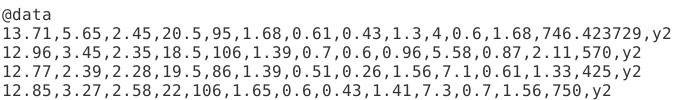
\includegraphics[scale=.32]{./figuras/image22.png}
	\caption{Base de datos 'wine'}
	\label{fig:normalize1}
	\end{figure}
	
	\begin{figure}[!htp]
	\centering
	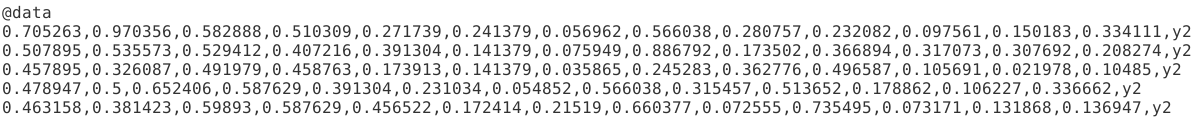
\includegraphics[scale=.32]{./figuras/image21.png}
	\caption{Base de datos 'wine' tras aplicar Normalize}
	\label{fig:normalize2}
	\end{figure}

	\subsection{ReplaceMissingValues}
	Reemplaza todo valor perdido, los cuales son representados con el signo '?', de los atributos nominales y numéricos.

	\begin{justify}
	\textbf{Uso} 
	\end{justify}

	Busca aquellos valores perdidos y los reemplaza con los valores de las modas y medias para dicho atributo.

	Para ilustrar el uso de este filtro se ha usado una pequeña base de datos que contiene notas de 3 asignaturas para varias instancias que son los alumnos, y se observa como los datos perdidos son reemplazados.

	
	\begin{justify}
	\textbf{Ejemplo}
	\end{justify}

	\begin{figure}[!htp]

	\centering
	  \subfloat[Base de datos 'notas' con valores perdidos]{
		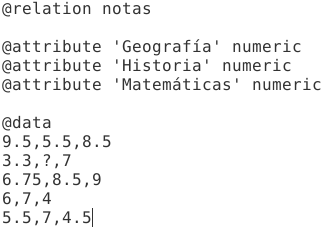
\includegraphics[scale=.32]{./figuras/image19.png}}
	  \subfloat[Media tras aplicar el filtro]{
		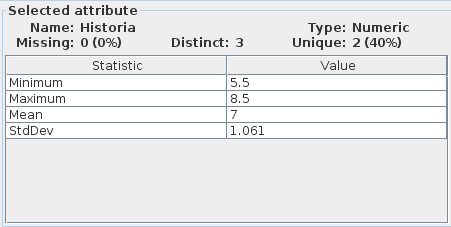
\includegraphics[scale=.32]{./figuras/image10.png}}
	\caption{Base de datos y media calculada tras aplicar ReplaceMissingValues}
	\end{figure}
  
	\begin{figure}[!htp]
	\centering
	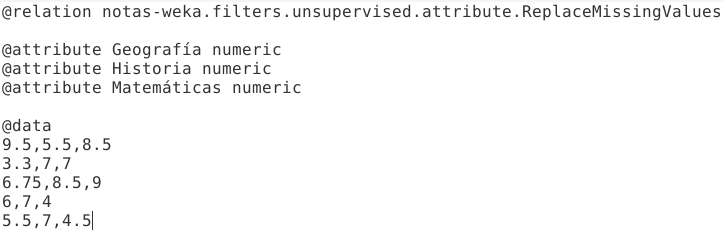
\includegraphics[scale=.32]{./figuras/image31.png}
	\caption{Fichero final con el valor perdido reemplazado}
	\end{figure}

\newpage
\subsection{RemoveUseless}
	\begin{justify}
		Elimina atributos nominales donde la varianza es muy grande o muy pequeña y que por tanto, no tienen utilidad.
	\end{justify}



	\begin{justify}
	\textbf{Uso} 
	\end{justify}
	Realiza el análisis y transformación de los componentes principales de los datos. Se usa junto con una búsqueda de Ranker. La reducción de la dimensionalidad se logra eligiendo suficientes vectores propios para tener en cuenta algún porcentaje de la varianza en los datos originales, por defecto 0.95.

	\begin{justify}
	\textbf{Ejemplo}
	\end{justify}
	Parar ilustrar este filtro se ha usado una pequeña base de datos que contiene un atributo nominal que representa un color, y 2 atributos numéricos que representan otros datos asociados. Se puede observar como el atributo nominal tiene un valor distinto para cada instancia, y por tanto, la varianza es la máxima, así pues el filtro actúa descartando dicho atributo nominal.
  

	\begin{figure}[!htp]
	\centering
	  \subfloat[Base de datos 'colores' con atributo nominal]{
		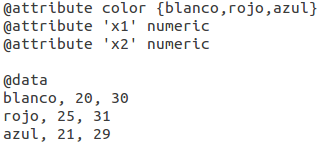
\includegraphics[scale=.45]{./figuras/image2.png}}
	  \subfloat[Fichero tras aplicar filtro]{
		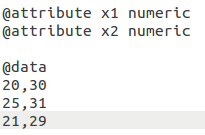
\includegraphics[scale=.5]{./figuras/image40.png}}
	\caption{Antes y después de aplicar RemoveUseless}
	\end{figure}




\newpage

	\subsection{PrincipalComponents}

	Realiza el análisis y transformación de las componentes principales de los datos.


	\begin{justify}
	\textbf{Uso} 
	\end{justify}

	La reducción de la dimensionalidad se logra eligiendo suficientes vectores propios para tener en cuenta algún porcentaje de la varianza en los datos originales (por defecto 0.95). El ruido de los atributos puede filtrarse transformándolo en el espacio de la Componente Principal, eliminando algunos de los vectores propios peores, y luego transformando de nuevo al espacio original.

	\begin{justify}
	\textbf{Ejemplo}
	\end{justify}

	
	\begin{figure}[!htp]
	\centering
	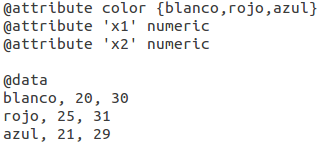
\includegraphics[scale=.42]{./figuras/image2.png}
	\caption{Base de datos 'colores'}
	\end{figure}
	
	\begin{figure}[!htp]
	\centering
	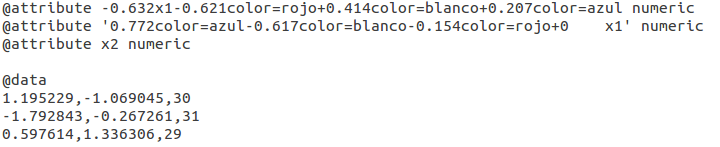
\includegraphics[scale=.42]{./figuras/image12.png}
	\caption{Fichero final tras aplicar PrincipalComponents}
	\end{figure}


\newpage

	\subsection{RandomProjection}
		Reduce la dimensionalidad de los datos proyectándolos en un subespacio de menor dimensión usando una matriz aleatoria con columnas de longitud unitaria.
	

	\begin{justify}
	\textbf{Uso} 
	\end{justify}
	
		Primero aplica el filtro NominalToBinary para convertir todos los atributos a numérico antes de reducir la dimensión. Conserva el atributo de marca de clase.

	\begin{justify}
	\textbf{Ejemplo}
	\end{justify}

		Como se muestra en la Figura 1.8 partimos de una base de datos con un atributo nominal de 3 posibles opciones 'Blanco', 'Rojo' y 'Azul' junto con un atributo numérico x1.
		Una vez aplicado el filtro, el primer atributo queda establecido en una matriz numérica de un subespacio menor. 

	\begin{figure}[!htp]
	\centering
	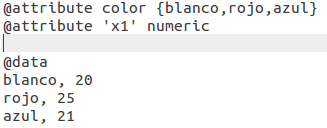
\includegraphics[scale=.42]{./figuras/image11.png}
	\caption{Base de datos 'colores' con un atributo numérico}
	\end{figure}
	
	\begin{figure}[!htp]
	\centering
	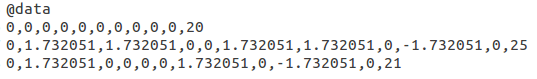
\includegraphics[scale=.42]{./figuras/image44.png}
	\caption{Fichero final tras aplicar RandomProjection}
	\end{figure}


\newpage
	\subsection{NominalToBinary}
	Convierte todos los atributos nominales en atributos binarios numéricos. 	

	\begin{justify}
	\textbf{Uso} 
	\end{justify}
	
	Un atributo con k posibles valores se transforma en k atributos binarios (0-1) si la clase es nominal. Los atributos binarios se dejan binarios. Si la clase es numérica, es posible que desee utilizar la versión supervisada de este filtro.

	\begin{justify}
	\textbf{Ejemplo}
	\end{justify}






\newpage
	\subsection{RemoveMissclassified}
	\begin{justify}
	Elimina aquellas instancias que han sido incorrectamente clasificadas, de modo que no existan valores atípicos.
	\end{justify}
	\begin{itemize}
		\item \textbf{Uso}
	\begin{justify}
	Permite escoger la marca de clase en la que se basan las clasificaciones erróneas, el clasificador 	sobre el que se basarán las clasificaciones erróneas, si el resultado será descartartado o aceptado, número de iteraciones, pliegues y umbral de error permisible.
	\end{justify}
		\item \textbf{Ejemplo}
	\end{itemize}

	\subsection{RemovePercentage}
	\begin{justify}
	Permite eliminar un porcentaje de la información de la base de datos.
	\end{justify}
	\begin{itemize}
		\item \textbf{Uso}
	\begin{justify}

	\end{justify}
		\item \textbf{Ejemplo}
	\end{itemize}

	\subsection{Resample}
	\begin{justify}
	Produce una submuestra aleatoria de un conjunto de datos utilizando el muestreo con reemplazo o sin reemplazo. 
	\end{justify}
	\begin{itemize}
		\item \textbf{Uso}
	\begin{justify}
	Se puede especificar el número de instancias en el conjunto de datos generado. Cuando se utilizan en modo por lotes, los lotes posteriores no son remuestrados.
	\end{justify}
		\item \textbf{Ejemplo}
	\end{itemize}

\newpage
\section{Filtros supervisados}
	%Son filtros que tienen en cuenta la variable marca de clase.	
	\subsection{AttributeSelection}
	\begin{justify}

	\end{justify}
	\begin{itemize}
		\item \textbf{Uso}
	\begin{justify}

	\end{justify}
		\item \textbf{Ejemplo}
	\end{itemize}
	
	\subsection{Discretize}
	\begin{justify}

	\end{justify}
	\begin{itemize}
		\item \textbf{Uso} 
	\begin{justify}

	\end{justify}
		\item \textbf{Ejemplo}
	\end{itemize}
 	
	\subsection{NominalToBinary}
	\begin{justify}

	\end{justify}
	\begin{itemize}
		\item \textbf{Uso}
	\begin{justify}

	\end{justify}
		\item \textbf{Ejemplo}
	\end{itemize}
	
	\subsection{SpreadToBinary}
	\begin{justify}

	\end{justify}
	\begin{itemize}
		\item \textbf{Uso}
	\begin{justify}

	\end{justify}
		\item \textbf{Ejemplo}
	\end{itemize}
 	
	
	\subsection{ClassBalancer}
	\begin{justify}

	\end{justify}
	\begin{itemize}
		\item \textbf{Uso}
	\begin{justify}

	\end{justify}
		\item \textbf{Ejemplo}
	\end{itemize}

	\subsection{Resampler}
	\begin{justify}

	\end{justify}
	\begin{itemize}
		\item \textbf{Uso}
	\begin{justify}

	\end{justify}
		\item \textbf{Ejemplo}
	\end{itemize}


\newpage
\section{Base de datos Wine}
	%\noindent Los objetivos principales que se persiguen en esta tesis doctoral son los siguientes:
 	
	\subsection{Detalles de la base de datos}
	
	\subsection{Modificación del fichero con nombres de atributo descriptivos}

	\subsection{Descripción de atributos y clases}

	\subsection{Tratamiento de elementos perdidos}

	\subsection{Diferencia entre Distinct y Unique}

	\subsection{Eliminar atributos identificadores}
	
	\subsection{Relaciones visualmente significativas en entorno Visualice}
	

\newpage
\section{Aplicación de 6 filtros a la base de datos}
	%\noindent Los objetivos principales que se persiguen en esta tesis doctoral son los siguientes:
 	
	\subsection{Filtro de selección de características}
	\begin{itemize}
		\item \textbf{Uso}
		\item Resultados:
		\item \textbf{Ejemplo}
	\end{itemize}

	\subsection{Filtro de selección de patrones}
	\begin{itemize}
		\item \textbf{Uso}
		\item Resultados:
		\item \textbf{Ejemplo}
	\end{itemize}

	\subsection{Filtro de filters/supervised/attribute/*}
	\begin{itemize}
		\item \textbf{Uso}
		\item Resultados:
		\item \textbf{Ejemplo}
	\end{itemize}

	\subsection{Filtro de filters/supervised/instance/*}
	\begin{itemize}
		\item \textbf{Uso}
		\item Resultados:
		\item \textbf{Ejemplo}
	\end{itemize}

	\subsection{Filtro de filters/unsupervised/attribute/*}
	\begin{itemize}
		\item \textbf{Uso}
		\item Resultados:
		\item \textbf{Ejemplo}
	\end{itemize}

	\subsection{Filtro de filters/unsupervised/instance/*}
	\begin{itemize}
		\item \textbf{Uso}
		\item Resultados:
		\item \textbf{Ejemplo}
	\end{itemize}



\newpage
\section{Conversión de todo atributo nominal a codificación binaria}


\newpage
\section{División de la base de datos en particiones}

	\subsection{División en 10-Holdout 75-25}
	\begin{itemize}
		\item \textbf{Uso}
		\item Resultados:
		\item \textbf{Ejemplo}
	\end{itemize}


	\subsection{División en 10-Fold}
	\begin{itemize}
		\item \textbf{Uso}
		\item Resultados:
		\item \textbf{Ejemplo}
	\end{itemize}

% 	A continuación y una vez descritos los objetivos de esta tesis doctoral, se exponen
% 	las aportaciones fundamentales incluidas en esta memoria:
% 	\begin{enumerate}
% 	\item Análisis y descripción de los aspectos más importantes en el uso de algoritmos
% 	evolutivos mono-objetivo y multi-objetivo híbridos, funciones de aptitud, DE y
% ensembles para el diseño de modelos de red para clasificación de
% 	patrones.
% 	\item Implementación de varias versiones de un AE memético mono-objetivo usando
% 	modelos de red puros e híbridos en capa oculta. Los resultados obtenidos están en
% 	consonancia con los	de otras	técnicas	frecuentemente citadas en Aprendizaje
% Automático (\textit{Machine Learning}, ML).
% 	\item Implementación de un MOEA	memético basado en dominancia de Pareto para diseñar
% 	modelos de	red para clasificación	de patrones.
% 	\item Implementación de varias versiones de un MOEA memético basado
% 	en dominancia de	Pareto y en la DE.
% 	\item Futura obtención de	padres virtuales en DE basados en
% 	los valores extremos y mejores individuos de la 	población.
% 	\item Estudio y análisis del uso de la mínima sensibilidad en la	clasificación de
% 	patrones	para problemas multiclase, como alternativa al uso de	curvas ROC y otras
% 	medidas
% 	de	rendimiento. Utilización de dicha función de aptitud en los algoritmos
% 	desarrollados obteniéndose resultados satisfactorios.
% 	\item Nueva representación en dos dimensiones de la bondad de un clasificador
% 	mediante la optimización simultánea de la precisión y la mínima sensibilidad.
% 	\item Aplicación de los algoritmos implementados en la resolución de problemas de
% 	clasificación reales de microbiología predictiva, teledetección y predicción de viento.
% % 	\item Inclusión los algoritmos implementados en KEEL,
% % 	ampliando de esta manera el abanico de técnicas de las que dispone la herramienta,
% % 	proporcionándole una mayor riqueza para labores científicas.
% 	\end{enumerate}

		\paginavaciacompleta
		\chapter{Clasificación y Regresión en WEKA}
\
\section{Algoritmo IB1 con 10-fold crossvalidation}
	\subsection{Visualización de la clasificación}
	\subsection{Interpretación de los resultados}

\newpage
\section{Algoritmo IBK (k=1, k=3, k=5) con 10-fold crossvalidation a 1}
	\subsection{Cálculo de media y desviación típica de las medidas}

	\begin{itemize}
		\item Accuracy:
		\item Kappa:
		\item RMSE:
		\item F-Measure:
		\item Media ponderada AUC:
	\end{itemize}

	\subsection{Visualización de la clasificación}
	\subsection{Interpretación de los resultados}
 
\newpage
\section{Base de datos house.arff}
	\subsection{Carga de la base de datos}
	
	\subsection{Variable Granite}
	\begin{itemize}
		\item Influencia en el modelo
		\item Conclusiones
	\end{itemize}
	
	\subsection{Variable binaria Bathroom}
	\begin{itemize}
		\item Influencia en el modelo
		\item Aplicación de algoritmo de regresión lineal
		\item Conclusiones
	\end{itemize}

	\subsection{Variable Bedrooms}
	\begin{itemize}
		\item Influencia en el modelo
		\item Conclusiones
	\end{itemize}

	\subsection{Variable HouseSize}
	\begin{itemize}
		\item Influencia en el modelo
		\item Aportación al modelo de regresión lineal
		\item Conclusiones
	\end{itemize}

\newpage
\section{Base de datos autoMpg.arff}
	
	\subsection{Aplicación del algoritmo LinearRegression con un 80-20}
	\subsection{Resultados obtenidos}
	\begin{itemize}
		\item Conclusiones
		\item Tablas comparativas
	\end{itemize}

	\subsection{Atributo que aporta más información de la variable dependiente}


	\subsection{Atributo que no aporta información al modelo}


	\subsection{Errores cometidos}
	\begin{itemize}
		\item Visualización
		\item Representación de las diferentes cruces
	\end{itemize}


	\subsection{Modificación del parametro attributteSelectionMethod}
	\begin{itemize}
		\item Conclusión en el nuevo modelo
		\item Análisis de menor peso de "weight" frente "acceleration"
	\end{itemize}

\newpage
\section{Método SimpleLinearRegression en base de datos autoMpg.arff}

	\begin{itemize}
		\item Respuesta
		\item Solución
		\item Visualización
		\item Comentario de resultados
	\end{itemize}

\newpage
\section{Algoritmos Logistic y SimpleLogistic}

	
	\subsection{Análisis}
		\begin{itemize}
			\item Conclusión
			\item Métricas
			\item Variables más influyentes (beta)
			\item Variables no usadas
			\item Visualización
			\item Asociación de fórmulas con modelos obtenidos según el algoritmo
		\end{itemize}

	\subsection{Visualización gráfica de errores cometidos}

	\subsection{Análisis de parámetros}

		\begin{itemize}
			\item maxBoostingIterations
				\begin{itemize}
					\item Análisis
					\item Modificación
				\end{itemize}

			\item heuristicStop
				\begin{itemize}
					\item Análisis
					\item Modificación
				\end{itemize}
		\end{itemize}
		%\paginavaciacompleta
		%\paginavaciasincuerpo
		%\chapter{Rendimiento en problemas de clasificación}\label{medidasRendimiento}
% \begin{quotation}
% 	\begin{small}
% 	\textit{El afán de perfección hace a algunas personas totalmente insoportables.}
% 	\end{small}
% 	\begin{flushright}Pearl S. Buck.\end{flushright}
% \end{quotation}

\section{Métricas de rendimiento}\label{2.1}
\noindent Uno de los problemas fundamentales en aprendizaje automático, (\textit{Machine
Learning},
ML), es la
clasificación en dos o más clases de un conjunto de ejemplos no conocido (conjunto de
generalización), en base al aprendizaje de un número de ejemplos
cuya	clase	si es conocida (conjunto de entrenamiento).

La evaluación del rendimiento es algo decisivo para obtener una medida del
rendimiento de un clasificador, en cuanto a los conjuntos de entrenamiento y
generalización. En ocasiones el proceso de diseño u obtención de un clasificador conlleva
una serie de etapas que implican un proceso iterativo, donde cada	iteración, puede alterar
considerablemente el clasificador que se está diseñando. Se requiere, por tanto, una
re-evaluación del clasificador en cada iteración para determinar cuál ha sido el	impacto
producido en su rendimiento, premiando, generalmente, aquellos cambios que lo han hecho
mejorar.

En la literatura existen diversas medidas para determinar el
rendimiento de un clasificador \cite{Duda2000,Caruana2004,Sokolova2009}, pero
antes de pasar a describir algunas de las más utilizadas, es conveniente definir lo que se
denomina matriz de contingencia o matriz de confusión de un clasificador.

Dado un problema de
clasificación multiclase con $Q$ clases, siendo $Q\geq2$, y $N$ patrones de entrenamiento
o generalización, la matriz de contingencia $M(g)$, de dimensión $Q\text{x}Q$, de un
clasificador $g$, está dada por:
\begin{displaymath}
\begin{tabular}{ccc}
&Clase Predicha & \\
$\mathbf{M(g)}=$ &$\left( \begin{array}{cccc}
n_{11} & n_{12} & \ldots & n_{1Q} \\
n_{21} & n_{22} & \ldots & n_{2Q} \\
\ldots & \ldots & n_{ii} & \ldots \\
n_{Q1} & n_{Q2} & \ldots & n_{QQ} \\
\end{array} \right)$ & \begin{sideways}\hspace{-0.8cm}Clase
Real\end{sideways} \\
\end{tabular}
\end{displaymath}
donde las filas indican la clase real de pertenencia y las columnas la pronosticada
por el clasificador.

Formalmente,  la matriz de confusión, $M(g)$, se puede definir como:
\begin{displaymath}
	 \mathbf{M(g)}=\left\{n_{ij};\sum_{i,j=1}^Q n_{ij}=N\right\}
\end{displaymath}
donde $n_{ij}$ representa el número de patrones asignados a la clase $i$, cuando
realmente pertenecen a la clase $j$. La diagonal corresponde a los patrones correctamente
clasificados para las $Q$ clases del problema, y los   $Q(Q-1)$	elementos fuera de la
diagonal principal corresponden a los errores de clasificación. En consecuencia, los
totales por fila indican
el número de patrones pertenecientes a cada una de las clases, y la suma de estos totales
es el tamaño de la muestra.

Si analizamos la matriz de confusión:
\begin{displaymath}
\left( \begin{array}{cccc}
n_{11} & \ldots & \ldots & n_{1Q} \\
\ldots & \ldots & n_{ij} & \ldots \\
\ldots & \ldots & \ldots & \ldots \\
n_{Q1} & \ldots & \ldots & n_{QQ} \\
\end{array}\right)
\end{displaymath}
,tenemos que:
\begin{eqnarray}
n_{i\circ} & = & \sum_{j=1}^Q n_{ij} \quad i=1,...,Q \nonumber \\
n_{\circ j} & = & \sum_{i=1}^Q n_{ij} \quad j=1,...,Q \nonumber
\end{eqnarray}
siendo $n_{i\circ}$ el total de patrones asociados la clase $i$ (suma por filas), y
$n_{\circ j}$ el número
de patrones predichos por el clasificador que se han clasificado como pertenecientes a la
clase $j$ (suma por columnas).

A partir de las expresiones anteriores, se puede deducir que $\displaystyle
\sum_{i=1}^Q n_{i\circ}=N$ y que $\displaystyle \sum_{j=1}^Q n_{\circ j}=N$. Por tanto,
las frecuencias relativas correspondientes al número de patrones de la clase $i$ sobre el
total de patrones viene dada por:
\begin{displaymath}
f_{i \circ}= \frac{n_{i \circ}}{N}
\end{displaymath}
Y la frecuencia relativa correspondiente al número de patrones que el clasificador ha
clasificado como clase $j$, con respecto al total de patrones viene dada por:
\begin{displaymath}
f_{\circ j}= \frac{n_{\circ j}}{N}
\end{displaymath}

En el caso de clasificación binaria (una clase positiva y una clase negativa), es decir,
con un valor de $Q=2$, la matriz de confusión está dada por:
\begin{displaymath}
\mathbf{M(g)} =
\left( \begin{array}{cc}
tp & fn\\
fp & tn\\
\end{array} \right)
\end{displaymath}
donde:
\begin{itemize}
\item $tp$ significa ``verdaderos positivos'', o número de elementos que son de
la clase positiva y que el clasificador ha clasificado como positivos.
\item $fn$ significa ``falsos negativos'', o número de elementos que son de la clase
positiva y que el clasificador a clasificado como negativos.
\item $fp$ significa ``falsos positivos'', o número de elementos de la clase negativa
que son clasificados como positivos.
\item $tn$ significa ``verdaderos negativos'', o número de elementos de la clase
negativa que son clasificados como negativos.
\end{itemize}

% Independientemente de que las medidas de rendimiento sean escalares, basadas en umbral,
%en
% ranking o en probabilidades, se podría diferenciar entre aquellas se utilizan solo para
% problemas binarios y aquellas que se pueden utilizar tanto en binarios como en
% multiclase.
%
% Por norma general, ninguna métrica es siempre mejor que otra a la hora de medir la
% bondad de un clasificador, ya que en muchas ocasiones depende del conjunto de
% patrones a clasificar el que una métrica nos proporcione un valor de precisión más o
% menos real sobre la capacidad que tiene un determinado clasificador. Además hay
%problemas
% en los que interesa maximizar o minimizar una medida dependiendo de nuestros
% intereses. Por ejemplo, no es lo mismo diagnosticar cáncer sobre una base de datos
% médica a un 20\% de pacientes que en realizadas no lo tienen que diagnosticar
% una carencia de cáncer a un 20\% de pacientes que en realidad si lo tienen. La
%siguientes
% secciones muestran una breve descripción de las medidas más comúnmente utilizadas.
% (¿¿¿NOS PUEDEN CRITICAR QUE NO DIGAMOS EN QUÉ SITUACIONES UTILIZAR UNA MÉTRICA Y EN
%CUÁLES
% OTRA Y PORQUÉ????)

\subsection{Métricas para problemas binarios}\label{metricasbinarios}
\noindent A continuación exponemos las métricas para problemas de clasificación binarios
que más se utilizan a la hora de obtener el rendimiento de un clasificador:
\begin{description}
\item[Precisión, C:] Efectividad global de un
clasificador o	 porcentaje	de patrones totales correctamente
clasificados. Es una medida que suele proporcionarse en tanto por
ciento.
\begin{displaymath}
C=\frac{tp+tn}{tp+fn+fp+tn}=\frac{tp+tn}{N}
\end{displaymath}
\item[Precisión positiva, P:] Porcentaje de patrones correctamente clasificados
de la clase positiva con respecto a todos los elementos que el clasificador predijo como
positivos. Dicho de otra forma sería el porcentaje de ejemplos que el clasificador ha
predicho como positivos y que realmente son positivos.
\begin{displaymath}
P=\frac{tp}{tp+fp}
\end{displaymath}
\item[Sensibilidad, TPR:] También se nombra por \textit{Recall} o
\textit{True Positive Rate} (TPR). Es el porcentaje de patrones correctamente
clasificados de la clase positiva con respecto al número total	de	elementos existentes de
esa clase, o también
se puede decir que es la efectividad del clasificador para identificar los
elementos de la clase positiva.
\begin{displaymath}
TPR=\frac{tp}{tp+fn}
\end{displaymath}
\item[Especificidad, Sp:] Porcentaje de patrones correctamente
clasificados de la
clase negativa con respecto al número total de elementos existentes de esa clase, o
también se puede decir que es la	efectividad del clasificador para identificar los
elementos de la clase negativa.
\begin{displaymath}
Sp=\frac{tn}{fp+tn}=1-FPR
\end{displaymath}
donde $FPR$ se define a continuación.
\item[Porcentaje de falsos positivos, FPR:] También se nombra por \textit{False Positive Rate}
(FPR), y se define como el porcentaje de
patrones incorrectamente clasificados de la clase negativa con respecto al número
total de elementos existentes de esa clase.
\begin{displaymath}
FPR=\frac{fp}{fp+tn}=1-Sp
\end{displaymath}
\item[\textit{Fscore}:] Es una medida que se basa en $P$ y $TPR$, y se puede
interpretar como una media ponderada de ambas. Es la relación entre los elementos
positivos y aquellos dados por el clasificador.
\begin{eqnarray}
Fscore&=&\frac{2}{\frac{1}{P}+\frac{1}{TPR}} =
2\cdot \frac{P\cdot TPR}{
	P+TPR}
% 	= \nonumber \\
% &=& \frac{(\beta^2+1)tp}{(\beta^2+1)tp+\beta^2fn+fp}
\nonumber
\end{eqnarray}
donde $\beta$ es un número real no negativo, en el caso de esta igualdad $\beta=1$.
%\item[\textit{F-measure:}] La medida F es (BUSCAR DESCRIPCION...)
%\begin{displaymath}
%F-measure=\frac{2}{\frac{1}{Precisión}+\frac{1}{Sensitivity}}
%\end{displaymath}
\item[Area bajo la curva, AUC:]
Capacidad del
clasificador para evitar una clasificación falsa, teniendo en cuenta tanto a la clase
positiva como a la negativa. Esta medida es una aproximación del área bajo una curva
ROC, y se puede ver como una transformación lineal del índice de Youden
\cite{Youden1950}. Se puede calcular de manera más precisa mediante el ``Algoritmo 2``
mostrado en \cite{Fawcett2006}. Concretamente el $AUC$ es una porción del área de un
cuadrado de lado la unidad,
estando su valor entre 0 y 1. Una aproximación al $AUC$ es la siguiente:
% Se puede demostrar que el área bajo la curva ROC es
% equivalente a la prueba de Mann-Whitney, una prueba no paramétrica aplicada a dos
%muestras
% independientes, cuyos datos han sido medidos al menos en una escala de nivel ordinal;
% también equivalente a la prueba de los signos de Wilcoxon.
% ESTA MEDIDA ESTA SACADA DEL PAPER ''a SYSTEMATIC ANALISYS OF PERFOMANCE
% FOR CLASSIFICATIONS TASK``, DICE QUE ES BINARIA Y YO HE SUPUESTO QUE SE REFIERE AL AUC
%DE
% LA CURVA ROC. POR FAVOR REVISADMELO. pONE QUE A VECES A ESTA MEDIDA SE LE LLAMA Balanced
% Accuracy (MIRAR FINAL DE LA PAGINA 429 DEL ARTICULO)
\begin{displaymath}
AUC=\frac{1}{2}\left(TPR+Sp\right)
\end{displaymath}
\item[Media geométrica, GM:] La media geométrica intenta maximizar
la precisión en las dos clases que componen un determinado problema de la forma más
balanceada posible. Aunque esta medida se puede extender para problemas multiclase su
utilización no es usual.
\begin{displaymath}
GM=\sqrt{TPR\cdot Sp}
\end{displaymath}
\end{description}

\subsection{Métricas para problemas multiclase}\label{metricasmulticlase}
\noindent A partir de la matriz de confusión multiclase mostrada en la sección \ref{2.1},
la sensibilidad de una clase $i$ en problemas multiclase, se define como, el número
de patrones correctamente predichos en esa clase con respecto al número total de patrones
de dicha clase (probabilidad de predecir correctamente un ejemplo de la clase $i$), y la
denotaremos por:
\begin{displaymath}
S_{i}=\frac{n_{ij}}{n_{i\circ}}, \qquad i=1,...,Q.
\end{displaymath}

La especificidad, $Sp$, de una clase $i$ en problemas multiclase, se define como, el número
de patrones correctamente predichos en esa clase con respecto al número total de patrones
predichos por el clasificador para esa clase. Hay que hacer notar que para problemas
binarios la
especificidad se refiere a la clase negativa, según está definida en la sección
\ref{metricasbinarios}:
\begin{displaymath}
Sp_{i}=\frac{n_{ii}}{n_{\circ j}}, \qquad j=1,...,Q.
\end{displaymath}

Teniendo en cuenta dicha matriz y las definiciones anteriores, las métricas más utilizadas
para problemas multiclase son las siguientes:
\begin{description}
	\item[Precisión, C:]  Al igual que en el caso de problemas binarios
	es el porcentaje de patrones correctamente clasificados. Es una medida que suele
	proporcionarse en tanto por ciento:
	\begin{displaymath}
	C=\left( \frac{1}{N}\right) \sum_{j=1}^Q n_{jj}
	\end{displaymath}
	Equivalentemente, $C$ puede expresarse como media ponderada de las
	sensibilidades:
	\begin{equation}\label{CenbaseS}
	C=\sum_{i=1}^Q \frac{n_{i\circ}}{N} S_{i}, \qquad i=1,...,Q\text{,}
	\end{equation}
	donde los pesos corresponden a las probabilidades "a priori" de cada clase.
	\item[Error cuadrático medio, MSE:] El error cuadrático
	medio es una medida que
	proporciona un promedio del error cometido por un clasificador entre los valores
	predichos, y los reales u observados. Los valores que puede tomar esta medida están
	entre 0 e $\infty$, y normalmente se utiliza en problemas de regresión, aunque hay
	autores que también la usan para clasificación \cite{Abbass2001,Abbass2002a}.
	\begin{displaymath}
	MSE=\left(\frac{1}{N}\right)\sum_{i=1}^N\left(\hat{Y}_{i}-Y_{i}\right)^2
	\end{displaymath}
	siendo $\hat{Y}_{i}$ la etiqueta estimada para el patrón $i$, e $Y_{i}$ la etiqueta real
	del	patrón $i$.

	En cuanto a los valores que puede tomar la variable $\hat{Y}_{i}$ y
	la variable $Y_{i}$, tanto en esta métrica como en las siguientes que se
	exponen dentro de esta sección, dependen de la interpretación que se haga de la/s
	salida/s que proporciona el clasificador que	estemos evaluando, y de los valores
	tomados como	verdaderos. Algunos ejemplos posibles de interpretación, aplicados en
	este	caso a ANNs, podrían ser los	siguientes: Una red
	neuronal	con varias salidas interpretadas de manera probabilística, donde el valor de
	cada salida indica la probabilidad de pertenencia a una clase determinada. Otra
	interpretación posible sería tener una red neuronal con una sola salida, comprendida
	entre 0 y 1, donde la pertenencia a una determinada clase se encuentra en un cierto
	rango	de esa salida. O incluso una red con varias salidas, donde cada una de ellas
	indica 0 o 1, dependiendo de si un patrón pertenece o no a una clase determinada. Por tanto,
	habrá
	que adaptar los valores $\hat{Y}_{i}$ y los valores $\hat{Y}_{i}$, de forma que se
	pueda aplicar la correspondiente métrica.
	\item[Raíz del error cuadrático medio, RMSE:] La raíz
	cuadrada	del error cuadrático
	medio, también proporciona un promedio del error cometido por un clasificador. Sus
	valores también están entre 0 e $\infty$.
	\begin{displaymath}
	RMSE=\sqrt{\left(\frac{1}{N}\right)\sum_{i=1}^N\left(\hat{Y}_{i}
	-Y_{i}\right)^2}
	\end{displaymath}
	\item[Entropía cruzada, E:] La entropía cruzada, es una función
	de error basada en
	las probabilidades de pertenencia de cada uno de los patrones de un conjunto de datos a
	cada una de las clases que componen un determinado problema. Los valores que puede
	tomar esta medida están	entre 0 e $\infty$.
	\begin{displaymath}
	E=-\left(\frac{1}{N}\right)\sum_{n=1}^N\sum_{l=1}^Qy_{n}^{(l)}\log
	g_{l}^{}(\mathbf{x}_{n})
	\end{displaymath}
	donde $y_{n}^{(l)}$ es igual a 1 si el patrón $n$ pertenece a la clase $l$, y 0 en caso
	contrario, y donde  $\displaystyle g_{l}^{}(\mathbf{x}_{n})$ es la probabilidad de que
	el patrón $n$ 	pertenezca a la clase $l$.
% 	\item[\textit{SEP (Standar Error Prediction):}] El error estándar de predicción es
% 	es una medida adimensional y se define como la	desviación típica de las diferencias
% 	entre los valores predichos y los valores reales. Al igual que el \textit{MSE} suele
% 	utilizarse en problemas de regresión.
% 	\begin{displaymath}
% 	SEP=\left( \frac{100}{\overline{Predicho}}\right)
% 	\sqrt{\left(\frac{1}{N}\right)\sum_{i=1}^N\left(Predicho(g)-Verdadero(g)\right)^2}
% 	\end{displaymath}
% 	donde $\overline{Predicho}$ es el valor medio de todas las salidas predichas por el
% 	clasificador.
% 	\item[Coeficiente de información mutua, IC:]
% 	Define la información aportada
% 	por una variable aleatoria sobre otra, o lo que es lo mismo, cuánto reduce la
% 	incertidumbre sobre una variable el conocimiento de la otra \cite{Baldi2000}. La
% 	expresión que se muestra a continuación se obtiene asumiendo que $\displaystyle
% 	H(X)=-\sum_{i}^{Q}X_{i}\log X_{i}$,
% 	y que $\displaystyle f=\frac{n_{i\circ}}{N}$, $\displaystyle k=\frac{n_{\circ j}}{N}$ y
% 	$\displaystyle n=\frac{n_{ij}}{N}$:
% 	\begin{eqnarray}
% 	IC&=&\frac{H(f)+H(k)-H(N)}{H(f)}=\nonumber \\
% 	&=&\frac{-\sum_{i=1}^Q\left(\frac{n_{i\circ}}{N}\log
% 	\frac{n_{i\circ}}{N}\right) -\sum_{i=1}^Q \left( \frac{n_{\circ j}}{N}\log
% 	\frac{n_{\circ j}}{N}\right) +\sum_{i,j=1}^Q \left( \frac{n_{ij}}{N}\log
% 	\frac{n_{ij}}{N}\right)}{-\sum_{i=1}^Q\left( \frac{n_{i\circ}}{N}\log
% 	\frac{n_{i\circ}}{N}\right)} \nonumber
% 	\end{eqnarray}
	\item[\textit{Generalized Squared Correlation}, GC$^{2}$:] La correlación
	cuadrática generalizada se puede considerar como una generalización para problemas
	multiclase del coeficiente de correlación de Matthews \cite{Matthew1975} para dos
	clases.
	\begin{displaymath}
	GC^2=\frac{1}{N\left(Q-1\right)}\sum_{i,j=1}^Q\frac{\left(
	n_{ij}-e_{ij}\right)^2}{e_{ij}}
	\end{displaymath}
	donde $\displaystyle e_{ij}=\frac{n_{i\circ}n_{\circ j}}{N}$	es el número esperado de
patrones en
	la posición	$ij$ de la matriz de confusión, teniendo como hipótesis que las asignaciones
	y	las	predicciones son independientes.
	\item[\textit{Macro-Average}, MAVG:] La macro-media se define como la media de las
	sensibilidades de cada clase, sin considerar la desviación típica. Da la misma
	importancia o peso a cada una de las clases de un problema.
	\begin{displaymath}
	MAVG=\frac{1}{Q}\sum_{i=1}^Q S_{i}
	\end{displaymath}
\end{description}
\newpage
\section{Curvas ROC}\label{curvasROC}
\noindent Cabe comentar por separado una de las técnicas más usadas habitualmente para
la comparación del rendimiento mostrado por dos o más clasificadores binarios, las
llamadas curvas
ROC \cite{Fawcett2006}. Dichas curvas son	una alternativa al
uso de la		precisión	y sus		problemas derivados \cite{Provost1997,Provost1998}, y
es	una buena	técnica para		comprobar si un
clasificador es mejor que	otro	en	términos de	la clase	minoritaria. Las curvas ROC son
gráficas en dos dimensiones, en la que se representan los errores de clasificación de la
clase negativa o $FPR$ en el eje horizontal, y la precisión de la clase positiva o
$TPR$ en el eje vertical. Las curvas ROC muestran
toda la información relacionada con el rendimiento de un clasificador, y permiten una
rápida visualización del tipo de relación entre los rendimientos de varios
clasificadores. El análisis de la curva ROC, o simplemente análisis ROC, proporciona
información para seleccionar los modelos posiblemente óptimos, y es también independiente
de la distribución de las clases en la población. El análisis ROC se relaciona de forma
directa con el análisis de coste-beneficio en toma de decisiones en diagnóstico médico.

Dentro de una gráfica ROC, un clasificador domina a otro mientras más arriba y más a la
izquierda se encuentre (ver figura \ref{ejemploROC}). El mejor método posible de
predicción se situaría en un punto en la esquina superior izquierda, o coordenada $(0,1)$
del plano ROC, representando un 100\% de sensibilidad (ningún falso negativo) y un 100\%  de
especificidad (ningún falso positivo). Este punto $(0,1)$ se denomina
clasificación perfecta. Por el contrario, una clasificación totalmente aleatoria daría
un punto a lo largo de la línea diagonal (línea de no-discriminación),
desde el extremo inferior izquierdo hasta el extremo superior derecho.

\begin{figure*}[htb]
\centering
\subfloat[Curva ROC]{\label{ejemploROC1}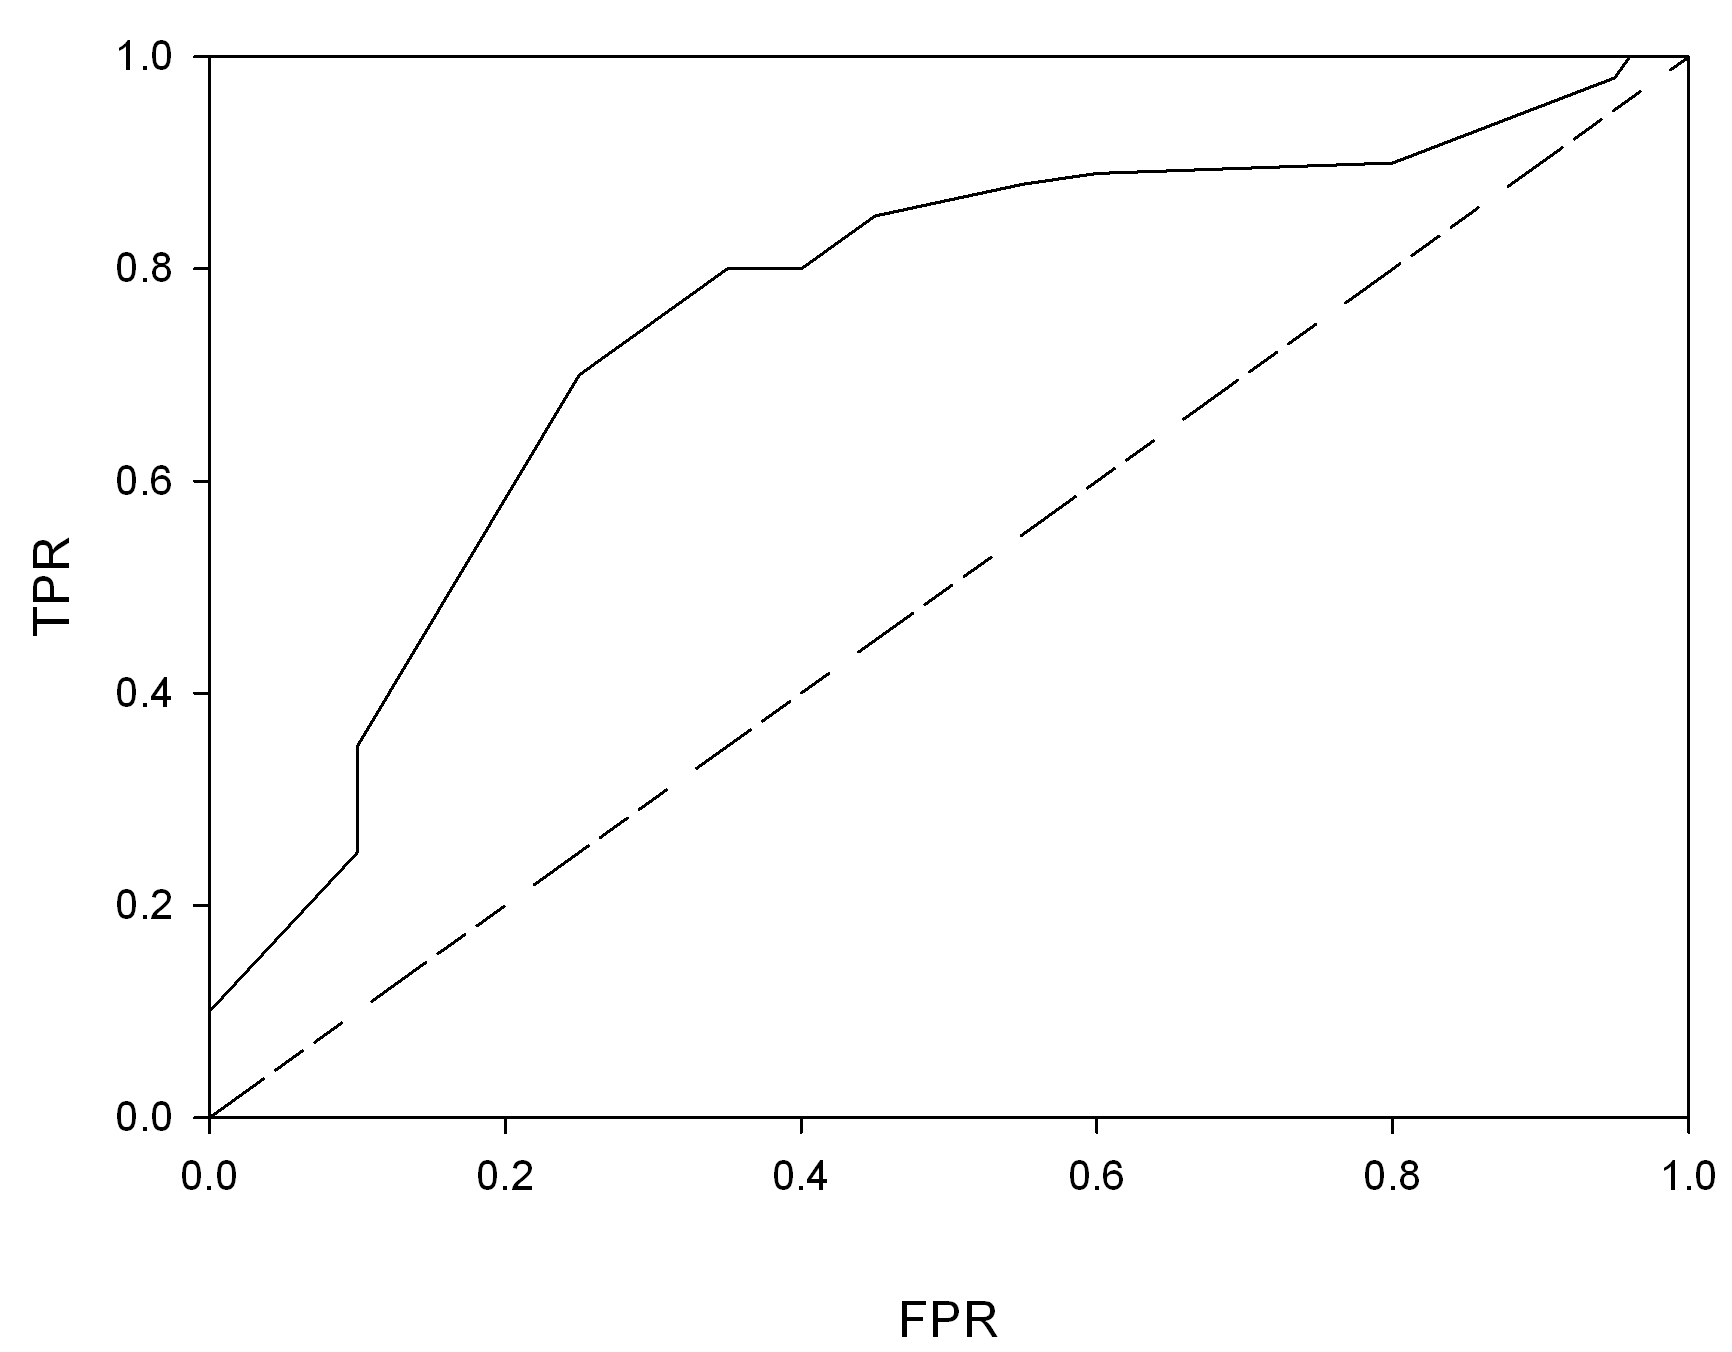
\includegraphics[width=.50
\textwidth]{figuras/curvaROC.jpg}}
\subfloat[Clasificador aleatorio]{\label{ejemploROC4}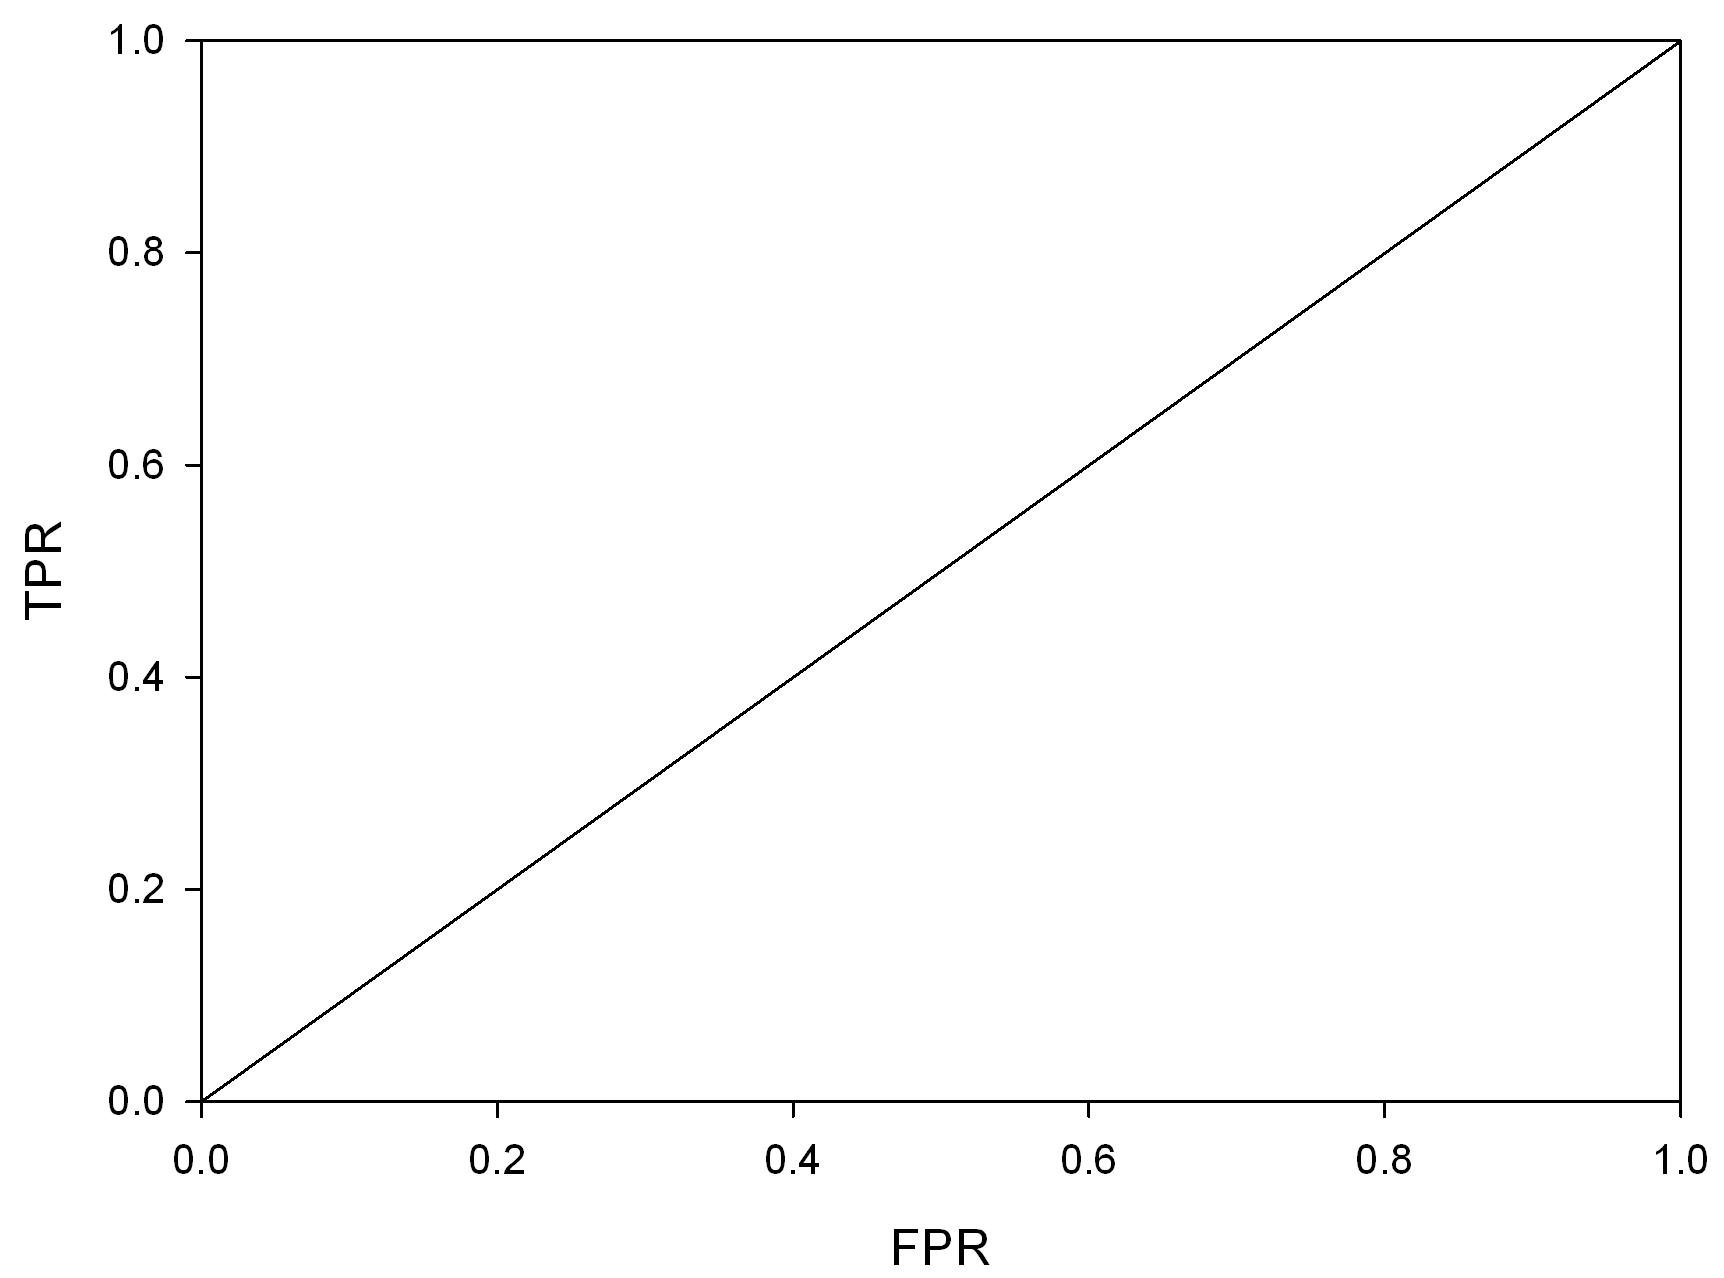
\includegraphics[width=.50
\textwidth]{figuras/curvaROCrealidad.jpg}} \\
\subfloat[Buen clasificador (alto
\textit{TPR} y bajo \textit{FPR})]{\label{ejemploROC2}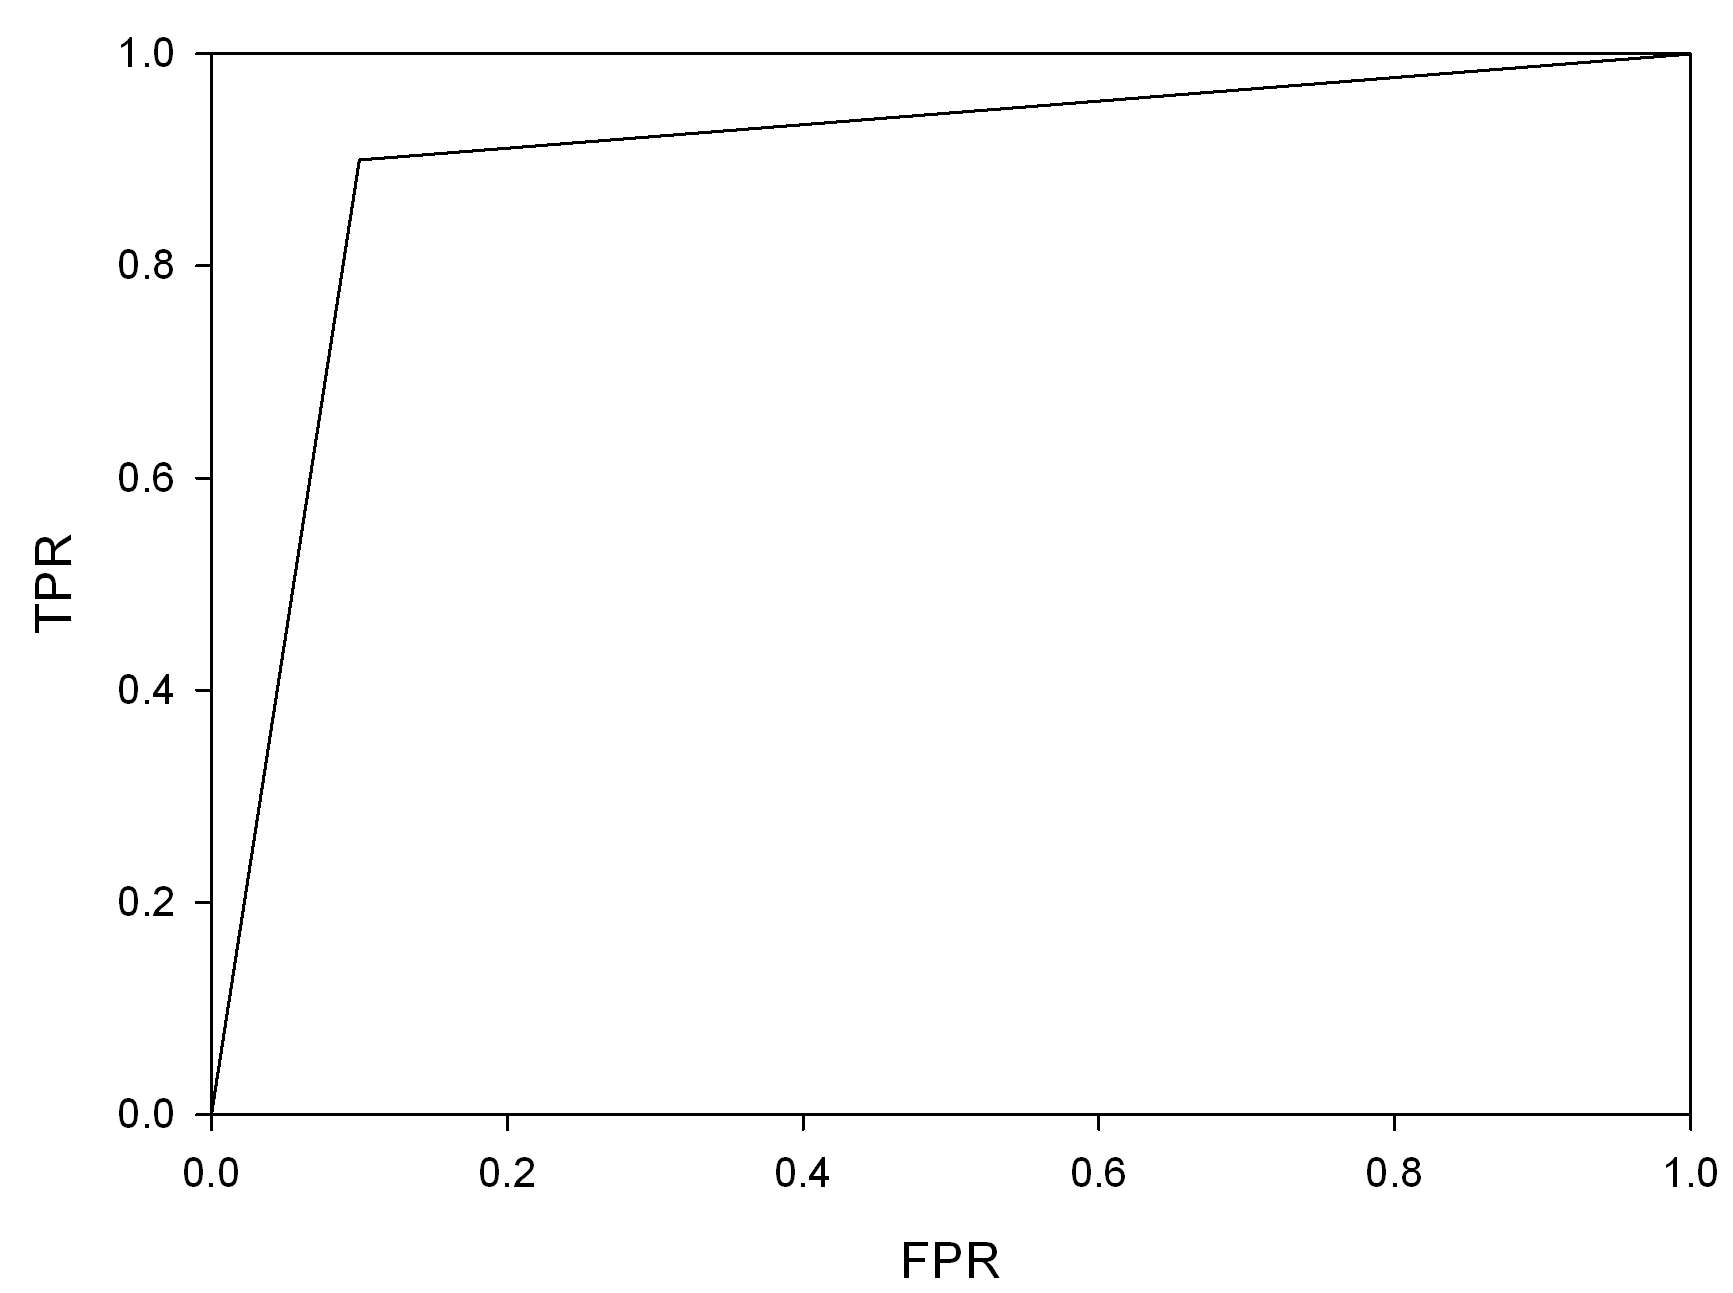
\includegraphics[width=.50
\textwidth]{figuras/curvaROCbueno.jpg}}
\subfloat[Mal clasificador, (bajo
\textit{TPR} y alto \textit{FPR})]{\label{ejemploROC3}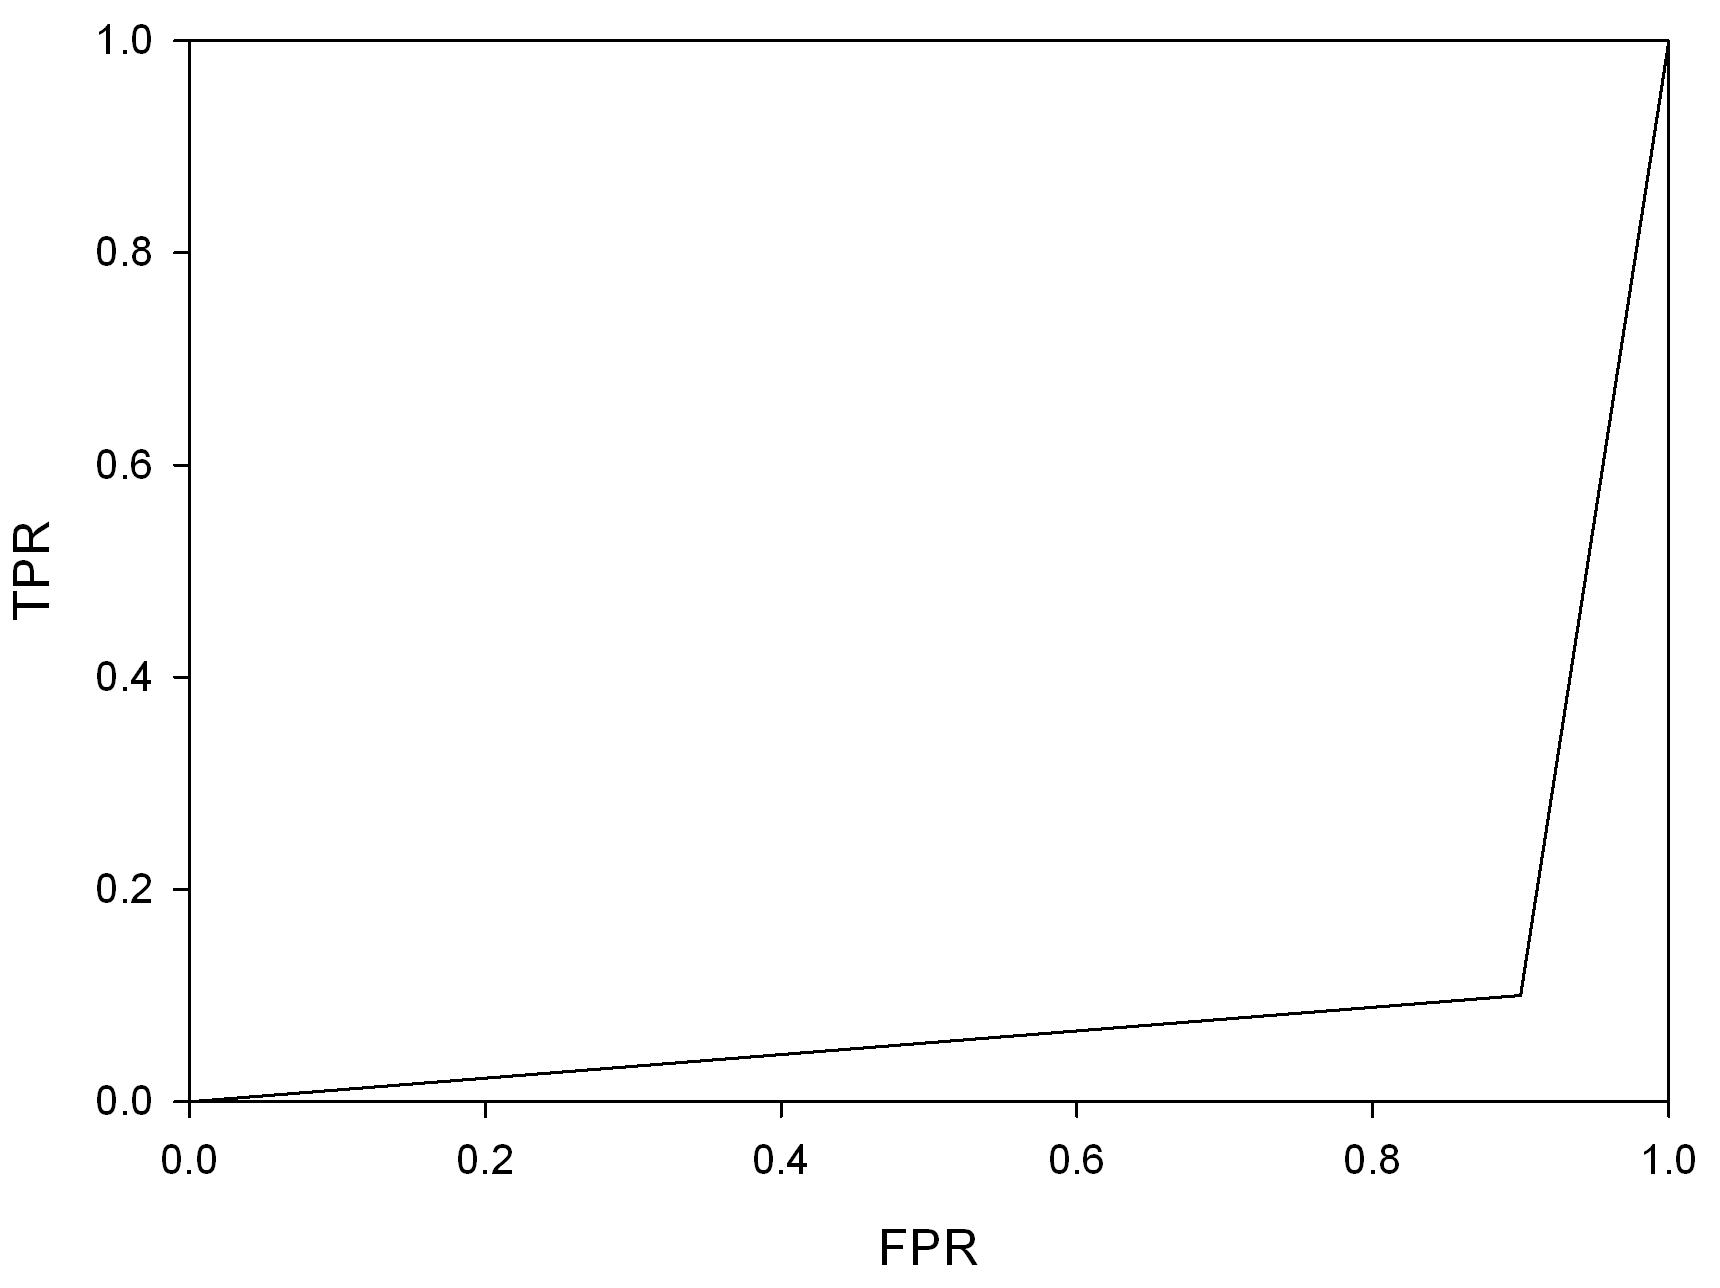
\includegraphics[width=.50
\textwidth]{figuras/curvaROCmalo.jpg}}

\caption{Ejemplos de curvas ROC}
\label{ejemploROC}
\end{figure*}

La extensión de las curvas ROC para dos clases a problemas multiclase
es interesante, ya que conferiría los beneficios del análisis ROC a más
problemas en reconocimiento de patrones. Se han realizado multitud de aproximaciones,
aunque actualmente no hay ningún análisis sobre
este tema que esté completamente consolidado \cite{Lachiche2003}. En \cite{Everson2006}, se
considera un problema de optimización	multi-objetivo donde el objetivo es minimizar
simultáneamente los $Q(Q-1)$ errores de	clasificación dados por los valores no
pertenecientes a la diagonal principal de la matriz de	confusión, donde el error se
define por $\displaystyle \frac{n_{ij}}{n_{i\circ}}$, para $i=1,2,...,Q$ y $j\neq i$. De
esta forma, el coste computacional crece en función del número de	clases. En
\cite{Langrebe2008}, se propone un algoritmo que a partir de la matriz de confusión
de un clasificador identifica las clases independientes y grupos de clases que
interactúan entre sí, permitiendo la descomposición de la matriz en un curva ROC con un
número bajo de grupos dimensionales. Esto reduce la complejidad computacional
considerablemente. La hiper-superficie ROC descompuesta se puede tratar como en el
caso ideal (dos clases), permitiendo realizar aproximaciones coste-beneficio y la
aproximación de Neyman-Pearson \cite{Edwards2004}, así como el volumen bajo la curva,
AUC. Otra manera de trabajar con problemas multi-clase es mediante el uso del
volumen sobre la superficie ROC (\textit{Volume under Surface}, VUS) \cite{Dreiseitl2007}
con curvas en 3-D \cite{Sahiner2008,He2008}. Así por ejemplo, en \cite{Mossman1999}, el
concepto de curvas ROC se extiende a cuestiones de diagnóstico médico con tres
posibles alternativas; se dibuja una superficie ROC en tres dimensiones para una
tarea de decisión tridimensional, añadiendo el VUS sobre la superficie ROC. De esta
manera, el VUS resume la precisión global del modelo,
similar al AUC de una curva ROC hecho sobre una tarea de
clasificación con dos	alternativas. La obtención de información en los puntos de la
superficie se puede	calcular de la misma forma que para curvas ROC bidimensionales, así,
se pueden comparar tres tipos de curvas ROC bidimensionales, en función de la información
de cada superficie.
% Otra aproximación en problemas multiclase consiste en considerar los
% errores de clasificación de cada una de las clases, es decir, el porcentaje de falsos
% positivos para
% cada clase, definidos por los elementos exteriores a la diagonal principal de la matriz
% de
% confusión, en lugar de los errores de clasificación de cada una de las otras clases.
% Así,
% el problema queda reducido a la minimización de los $Q$ objetivos definidos por
% \begin{displaymath}
% \frac {\sum_{i\neq j}^{Q}n_{ij}}{n_{i\circ}}, \quad i=1,,2,...,Q.
% \end{displaymath}

De forma general, en el caso de utilizar MOEAs para la resolución de problemas multiclase
mediante aproximaciones ROC, se deben tener presentes algunos inconvenientes:
\begin{enumerate}
	\item La dimensión de los frentes de Pareto crece junto con el número de clases del
	problema, haciendo extremadamente difícil encontrar soluciones que dominen al resto.
	Esto es debido a que mientras más crezca el espacio
	de objetivos, más complicado es que una solución sea mejor que otra en al menos uno
	de los objetivos e igual en los demás, según la definición de no-dominancia
	\cite{Coello2007}.
	\item El coste computacional a la hora de obtener modelos de red también aumenta
	considerablemente, ya que el número de comparaciones y operaciones a realizar para
	obtener individuos no dominados crece exponencialmente, cuadráticamente o
	linealmente con el número de clases.
	\item Los	sucesivos	frentes de Pareto que conforman la población de
	soluciones tendrán	cada vez menos individuos, a medida que aumente el número de
	objetivos ($Q(Q-1)$ errores de	clasificación) a optimizar en el problema. Esto
	hace que una de las principales	ventajas de los MOEAs, que es el proporcionar al
	experto un amplio abanico de	soluciones igualmente válidas, no se aproveche.
	\item Trabajar con más de dos objetivos tiene la desventaja de que el número
	de dimensiones de las representaciones gráficas aumenta, y por tanto sea más
	difícil su análisis e interpretación.
	\end{enumerate}

% Para reducir estos inconvenientes, normalmente lo que se intenta es hacer una
% aproximación
% trabajando solo con los errores de clasificación
% para cada clase, es decir, los falsos positivos en lugar del error de clasificación en
% cada una de	las otras clases (definido por los elementos que hay fuera de la diagonal
% principal	de la matriz de confusión). Esta propuesta reduce la dimensión del
% problema desde el	punto de vista del número de objetivos, sin embargo, esta
% proyección solo suele ser efectiva para problemas de tres clases.

\section{Mínima Sensibilidad-Precisión ($MS,C$)}\label{ms-c}
\noindent Teniendo en cuenta las definiciones dadas en la sección
\ref{metricasmulticlase}, se puede definir la Mínima Sensibilidad, $MS$, de un
clasificador $g$, como el mínimo valor de las sensibilidades de cada una de las clases
de un problema:
\begin{displaymath}
MS=min\left\lbrace S_{i};i=1,...,Q\right\rbrace
\end{displaymath}

La principal ventaja de las medidas de rendimiento mencionadas en la sección \ref{2.1}
es su simplicidad, ya que resumen o recogen de manera más o menos precisa, en un solo
valor numérico, el rendimiento de un clasificador. Sin embargo, esta simplicidad es a la
vez un punto débil, ya que un mismo valor proporcionado por uno de esos indicadores puede
representar diferentes situaciones. Si se asume que todos los errores de clasificación son
igualmente costosos, y que no hay preferencia ni penalización por un determinado conjunto
de patrones, un buen clasificador debería obtener un alto nivel de precisión global, así
como un aceptable nivel de precisión para cada clase. La precisión no puede capturar todos
los aspectos de
comportamiento	de dos clasificadores diferentes \cite{Provost1997,Provost1998}, y no es
suficiente, en algunos casos, para	determinar la calidad de un clasificador.

En esta tesis proponemos una medida de rendimiento bidimensional, de manera que pueda estar
en un punto intermedio entre las medidas unidimensionales como $C$, y las
multidimensionales dadas por los errores de clasificación, definidos por los elementos
exteriores a la diagonal principal de la matriz de confusión. Así, se intentan evitar los
problemas y limitaciones de las medidas unidimensionales, sin sufrir los
problemas relacionados con las medidas en $Q$ dimensiones (inconvenientes comentados
anteriormente de las aproximaciones
basadas en los $Q(Q-1)$ porcentajes de mala clasificación). Consideremos por tanto, como
compromiso entre ambas posibilidades, las medidas $(MS,C)$ como medidas que expresan dos
características asociadas con un clasificador: el rendimiento global, $C$, y el porcentaje
de aciertos de la clase peor clasificada, $MS$.

La selección de $MS$ como una medida complementaria de $C$ se puede justificar
considerando que la ecuación (\ref{CenbaseS}) es la media ponderada de las
sensibilidades de cada una de las $Q$ clases. Desde un punto de vista estadístico, $C$ es
una medida buena y representativa del conjunto de las sensibilidades, si éstas son lo
suficientemente homogéneas, aunque no será una medida representativa si las sensibilidades
están muy dispersas. Teniendo en cuenta este hecho, una medida complementaria de $C$ se
podría obtener considerando alguna medida que minimizase dicha dispersión, por ejemplo, el
rango $R=max\{S_{i}\}-min\{S_{i}\}$ podría ser una posible elección. Esta minimización
se puede	alcanzar si se minimiza $max\{S_{i}\}$ o se maximiza $min\{S_{i}\}$. La primera
opción no es apropiada, ya que $C$ aumenta si las sensibilidades aumentan,
por tanto la segunda alternativa es la más apropiada. De esta forma $MS=min\{S_{i}\}$, se
puede	considerar como la medida complementaria de $C$, cuyo valor hay que maximizar.

\subsection{Ejemplos}
La consideración simultanea de $MS$ y $C$ puede ayudar a clarificar los
errores y confusión que generan por si solas las medidas unidimensionales, veamos algunos
ejemplos y contra-ejemplos sobre ello:

\textbf{Ejemplo 1 (inadecuación de $C$):} Consideremos un problema de
clasificación con tres clases, y las matrices de confusión, $A$ y $B$, asociadas a dos
clasificadores, $f$ y $g$.
\begin{equation} \nonumber
A=\left( \begin{array}[c]{ccc}
60 & 0 & 0\\
0 & 30 & 0\\
5 & 4 & 1
\end{array}\right) \quad
B=\left( \begin{array}[c]{ccc}
57 & 3 & 0\\
0 & 30 & 0\\
5 & 1 & 4
\end{array}\right)
\end{equation}
Ambos clasificadores tienen la misma precisión $\displaystyle C=\frac{91}{100}=0.91$. Sin
embargo, el rendimiento en las clases es muy diferente. La $MS$ del clasificador
$f$ es $\displaystyle S_{f}= min\left\lbrace 1,1,0.1\right\rbrace=0.1 $, mientras que la
$MS$ de $g$ es $\displaystyle S_{G}= min\left\lbrace 0.95,1,0.4\right\rbrace=0.4 $. Este
ejemplo muestra claramente que la precisión no es una medida óptima para evaluar la
calidad de un clasificador, ya que no tiene en cuenta la clasificación individual de las
clases, sino un resultado general.

En problemas altamente desbalanceados, por norma general, hay un error no uniforme a
favor de la clase minoritaria (a menudo la clase de mayor interés). De esta manera, los
clasificadores que optimizan la precisión son cuestionables, en cuanto a que raramente
predicen de manera adecuada la clase minoritaria.

\textbf{Contraejemplo 1:} La $MS$ de un clasificador $f$ es $\displaystyle
MS_{f}=Min\left\lbrace 1,1,0.1\right\rbrace=0.1$, mientras que la de un clasificador
$g$ es $\displaystyle MS_{g}=Min\left\lbrace 0.95,1,0.4\right\rbrace=0.4$. En la figura
\ref{marianoejemplo1} se pueden ver los clasificadores $f$ y $g$ dentro del plano
$(MS,C)$. Claramente se puede considerar el clasificador $g$ mejor que el $f$.

\begin{figure*}[!htb]
\centering
\subfloat[]{\label{marianoejemplo1}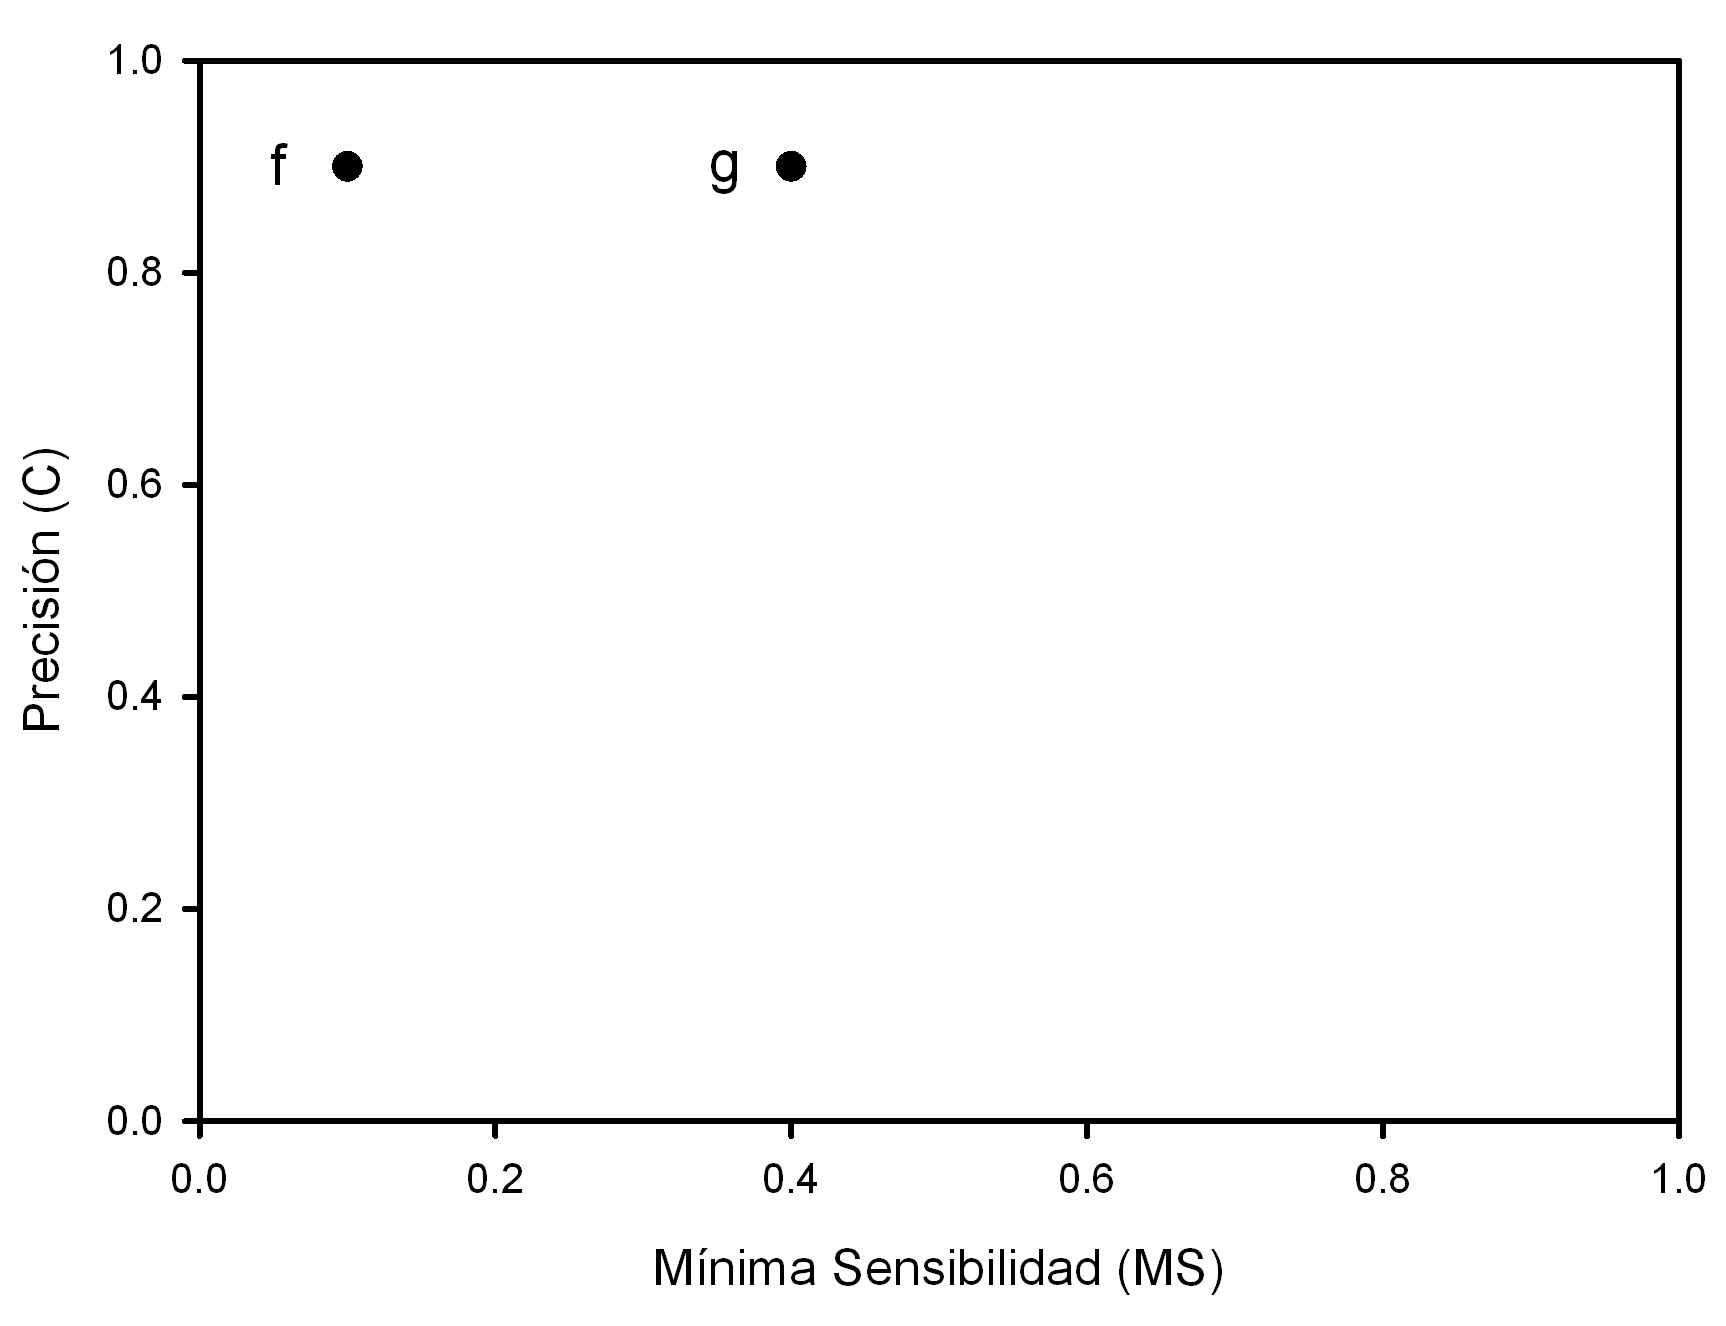
\includegraphics[width=.50
\textwidth]{figuras/articuloMarianoFigure2.jpg}}
\subfloat[]{\label{marianoejemplo3}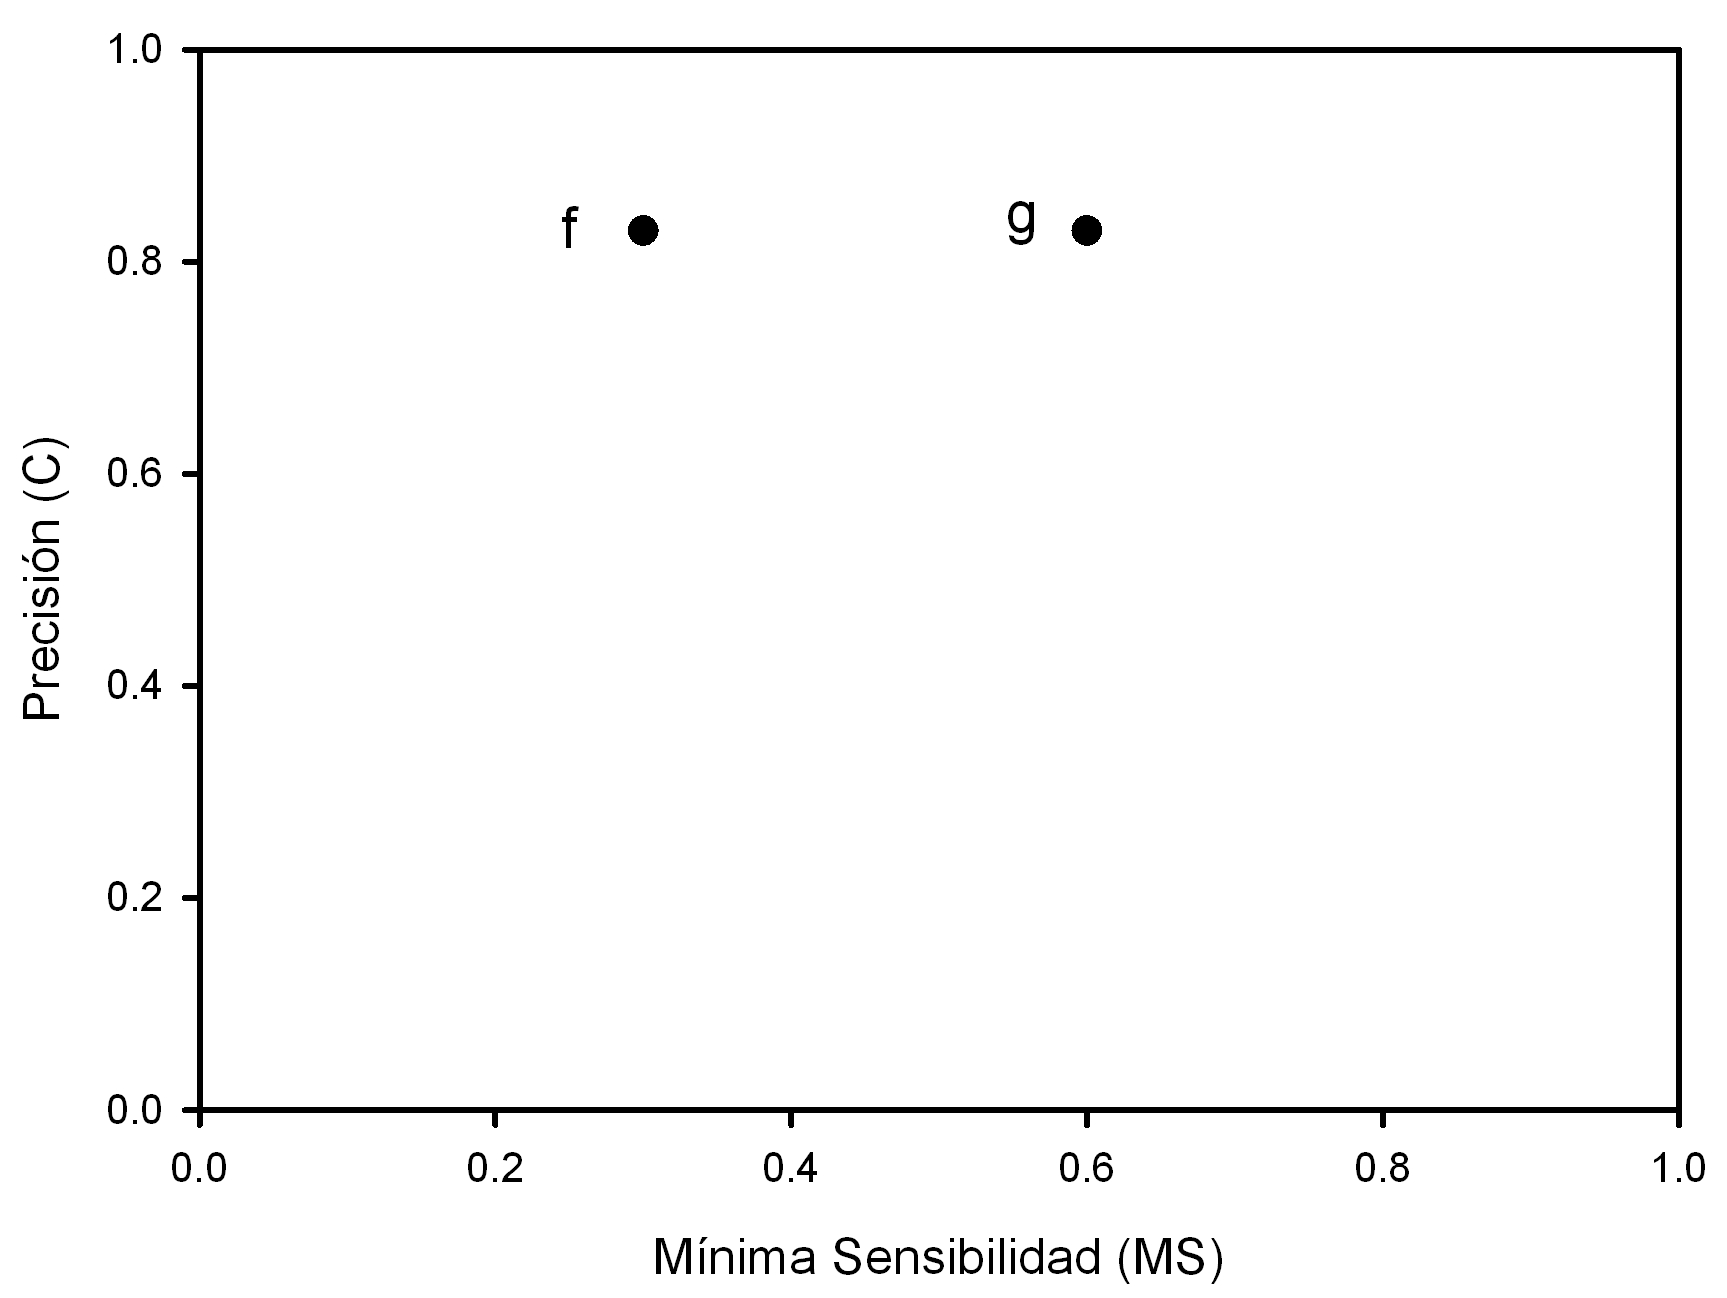
\includegraphics[width=.50
\textwidth]{figuras/articuloMarianoFigure4.jpg}} \\
\subfloat[]{\label{marianoejemplo2}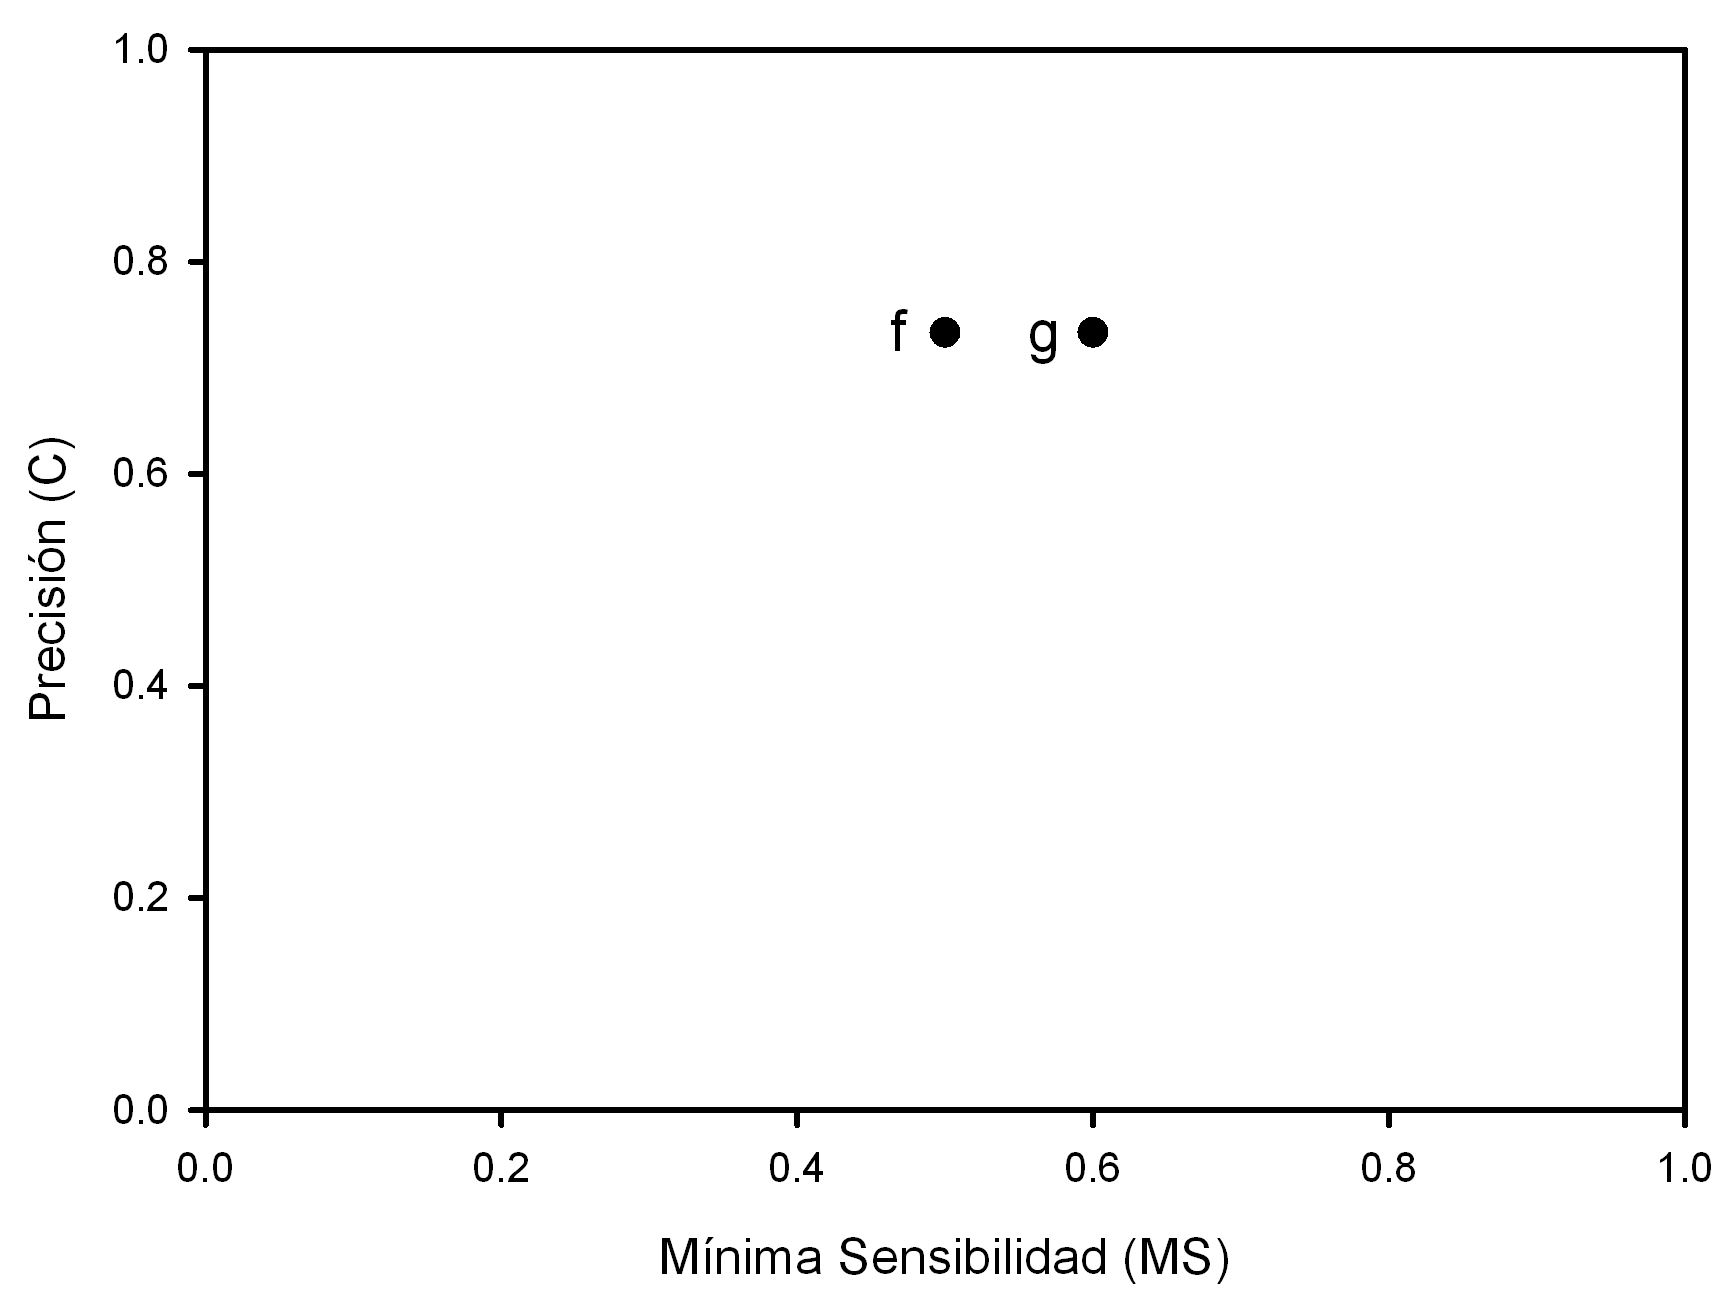
\includegraphics[width=.50
\textwidth]{figuras/articuloMarianoFigure3.jpg}}
\subfloat[]{\label{marianoejemplo4}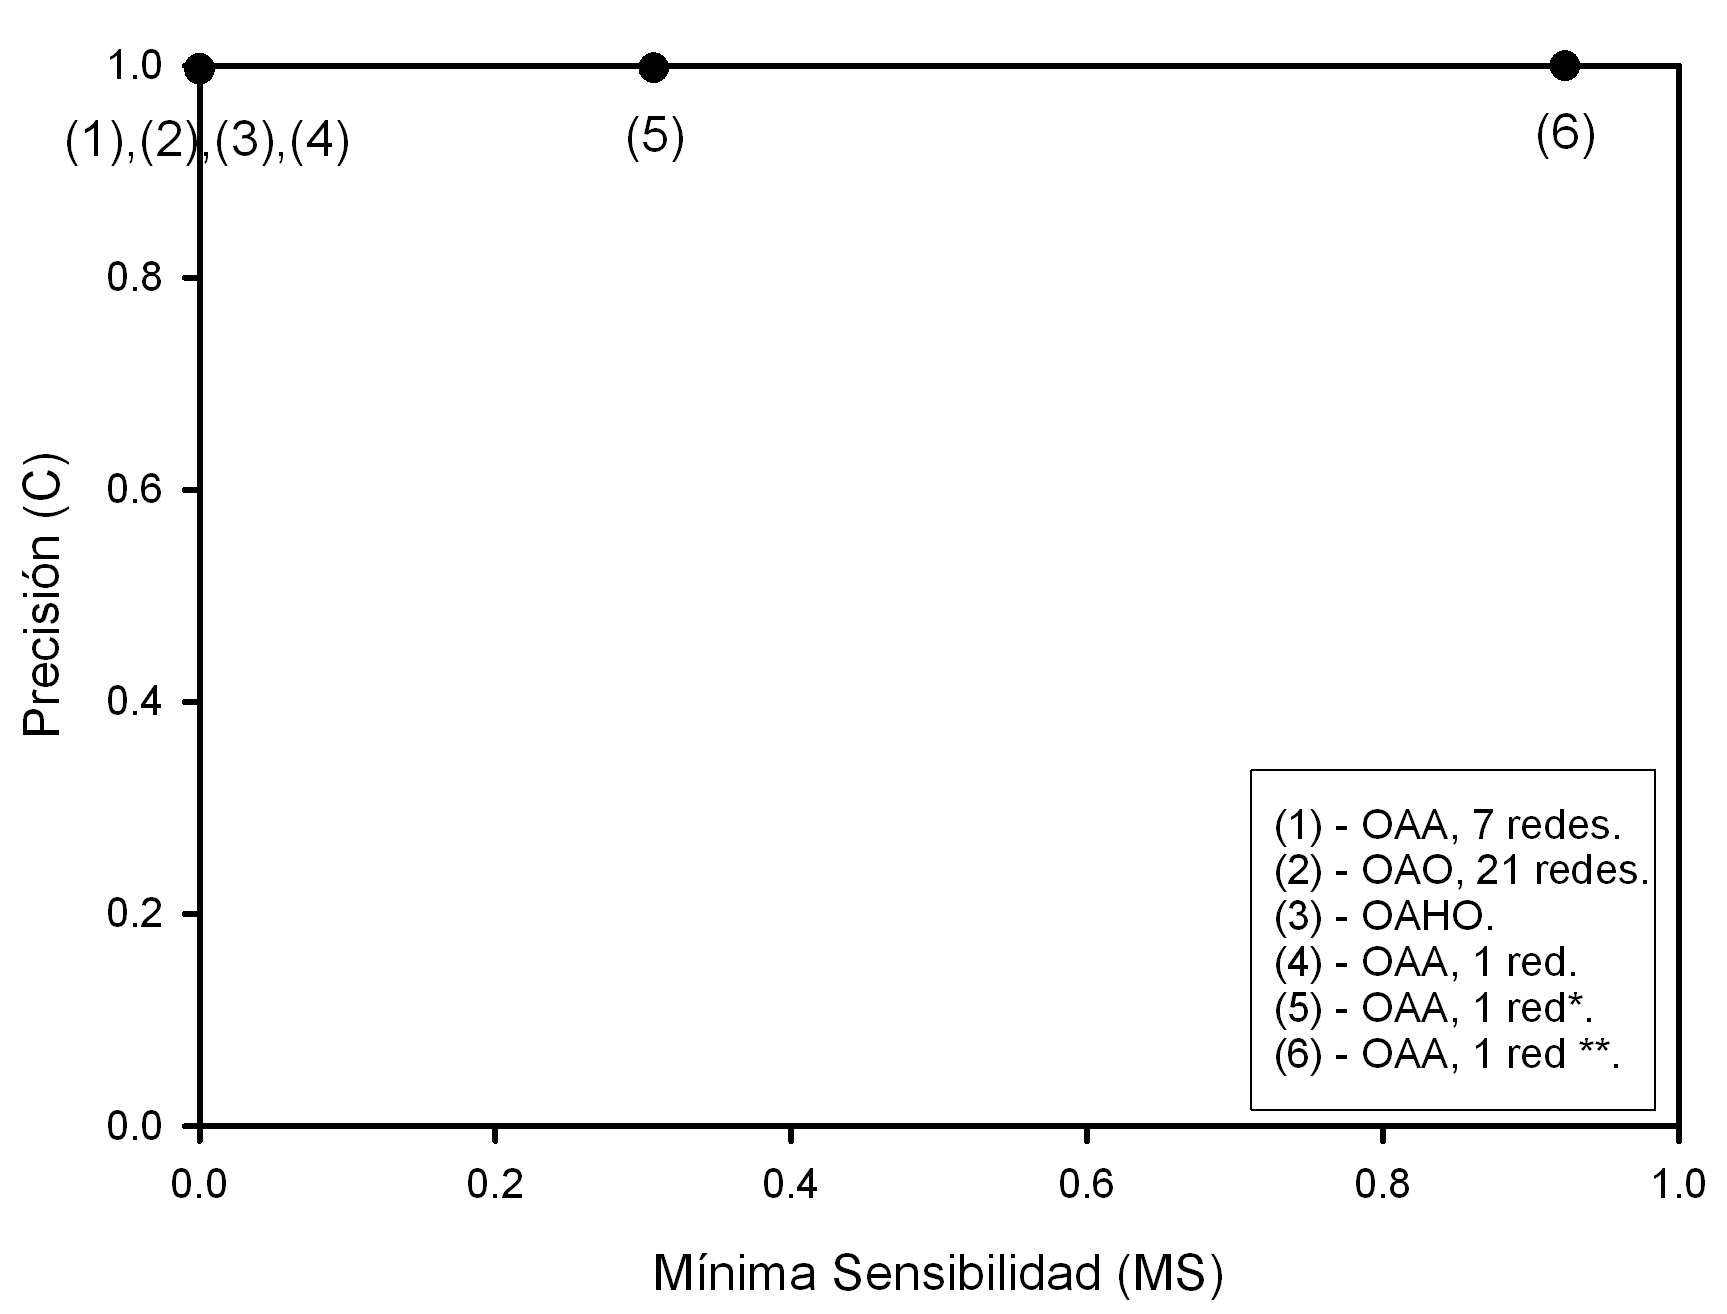
\includegraphics[width=.50
\textwidth]{figuras/articuloMarianoFigure5.jpg}}
\caption{Clasificadores $f$ y $g$ en el plano $(MS,C)$.}
\label{marianofigures}
\end{figure*}

\textbf{Ejemplo 2 (Inadecuación de la macro-media):} Permítanos considerar un problema de
clasificación con cinco clases de tamaño 250, 150, 100, 100 y 10 respectivamente, y las
correspondientes matrices de confusión, $A$ y $B$,  asociadas a dos clasificadores $f$ y
$g$, con los siguientes elementos de la diagonal principal:
\begin{displaymath}
diag(A)=\left( 155,150,99,99,3\right); \quad
diag(B)=\left( 200,150,83,67,6\right),
\end{displaymath}
pudiendo tomar los valores exteriores a la diagonal principal cualquier valor.

Ambos clasificadores tienen la misma $MAVG$. Las sensibilidades para cada clase en el
clasificador $f$ son $\displaystyle S_{1}=0.62, S_{2}=1, S_{3}=0.99, S_{4}=0.99,
S_{5}=0.3$ y las del clasificador $g$ son $\displaystyle S_{1}=0.8, S_{2}=1, S_{3}=0.83,
S_{4}=0.67, S_{5}=0.6$. Así, la macro media de $f$ y $g$ es $\displaystyle \left( 1/5
\cdot \sum_{i=1}^5 S_{i}\right) =0.78$, con lo que no distingue a los clasificadores.

\textbf{Contraejemplo 2:} Los clasificadores del ejemplo 2 tienen la misma $MAVG$
y las precisiones de ambos son $\displaystyle \frac{506}{610}=0.829$, la $MS$ de
$f$ es $MS_{f}=0.3$, mientras que la $MS$ del clasificador $g$ es $\displaystyle
MS_{g}=0.6$, por tanto el clasificador $g$ es mejor que el clasificador $f$. En la
representación gráfica mostrada en la figura \ref{marianoejemplo3} se puede ver como $g$
domina a $f$.

\textbf{Ejemplo 3 (Inadecuación de la media geométrica):} Permítanos considerar un
problema de clasificación con 300 patrones y tres clases de 100, 100 y 100 patrones
respectivamente. Sean $A$ y $B$ las matrices de confusión correspondientes a los
clasificadores $f$ y $g$, de forma que sus diagonales principales vienen dadas por:
\begin{displaymath}
diag(A)= (50,80,90); \quad diag(B)= (60,60,100)
\end{displaymath}
Las sensibilidades para cada clase en el clasificador $f$ son $S_{1}=0.5, S_{2}=0.8,
S_{3}=0.9$ y para el clasificador $g$ son $S_{1}=S_{2}=0.6, S_{3}=1$, y la media
geométrica de los dos es $GM(f)=GM(g)=0.711$.

\textbf{Contraejemplo 3:} Los clasificadores del ejemplo 3 poseen la misma precisión
$C=0.733$. La $MS$ del clasificador $f$ es $MS_{f}=min\left\lbrace
0.5,0.8,0.9\right\rbrace = 0.5$, mientras que la de $g$ es $MS_{g}=min\left\lbrace
0.6,0.6,1\right\rbrace = 0.6$, por tanto podríamos decir que el clasificador $g$ es mejor
que el clasificador $f$ (ver figura \ref{marianoejemplo2}).

\textbf{Ejemplo 4:} Para este ejemplo hemos considerado los resultados obtenidos por
diferentes metodologías en \cite{Ou2007}. Los autores utilizan cuatro sistemas de ANNs con distinto
número de redes para la clasificación de patrones:
un sistema basado en un esquema uno contra uno (\textit{One Against One} OAO), un sistema
uno contra todos (\textit{One Against All}, OAA) para redes binarias, una red neuronal
simple entrenada con un esquema OAA, y un sistema de modelado uno contra el mejor orden
(\textit{One Against Higher Order}, OAHO). Estas metodologías se aplican a dos conjuntos
de datos desbalanceados, \textit{Glass} y \textit{Shuttle}. A partir de la tabla
\ref{tablaEjemplo4}, que se corresponde con la tabla 4 del citado artículo, podemos
representar los clasificadores obtenidos en el plano $(MS,C)$ para el conjunto de datos
\textit{Shuttle} (figura \ref{marianoejemplo4}). Dichos resultados muestran que la
metodología OAA con una red obtiene un clasificador dentro del plano $(MS,C)$ que domina a
los demás y que la precisión no distingue prácticamente entre las 6 metodologías.

\begin{table}[!htb]
\caption{Mínima sensibilidad, $MS$, y precisión, $C$, para los clasificadores en el
conjunto de datos Shuttle.}
\label{tablaEjemplo4}
\centering
\begin{tabular}{p{4cm}p{3.2cm}p{2.8cm}} \hline
\rowcolor[rgb]{0.70,0.85,1}\textbf{Metodología} & $\mathbf{MS}$ & $\mathbf{C}$\\ \hline
\rowcolor[rgb]{0.86,0.94,1}OAA, 7 redes & 0 & 0.9963\\
\rowcolor[rgb]{0.86,0.94,1}OAO, 21 redes & 0 & 0.9969\\
\rowcolor[rgb]{0.86,0.94,1}OAHO & 0.076 & 0.9969\\
\rowcolor[rgb]{0.86,0.94,1}OAA, 1 red & 0 & 0.9963\\
\rowcolor[rgb]{0.86,0.94,1}OAA, 1 red * & 0.307 & 0.9977\\
\rowcolor[rgb]{0.86,0.94,1}OAA, 1red ** & 0.923 & 0.9977 \\ \hline
\multicolumn{3}{l}{* Con duplicación previa de los datos de la clase minoritaria.} \\
\multicolumn{3}{l}{** Entrenamiento con datos de la clase minoritaria e incremento}
\\
\multicolumn{3}{l}{de la capacidad de la red para entrenamiento posterior con datos} \\
\multicolumn{3}{l}{dinámicos.}
\end{tabular}
\end{table}

\section{Propiedades de las medidas $(MS,C)$}\label{propiedades}
Previo a definir las propiedades de las medidas $(MS,C)$, es necesario establecer cuál
es la relación entre ambas:

Consideremos un problema de clasificación con $Q$ clases, siendo $C$ y $MS$ las
medidas asociadas a un clasificador $g$, y $p^*$ la mínima de las frecuencias relativas
de cada clase calculadas ''a priori``. De esta forma, podemos representar los valores
de $MS$ y $C$ en un eje de coordenadas, concretamente $MS$ en el eje $X$ y $C$ el eje $Y$,
de manera que se puede visualizar fácilmente el rendimiento de un clasificador, sin tener
en cuenta el número de clases	que tenga el problema.

Un punto en el plano $\left(MS,C\right)$ domina a otro si tiene un mayor valor de $C$ e
igual o mayor valor de $MS$, o si tiene mayor valor de $MS$ y mayor o igual de $C$.
Idealmente, a partir de la desigualdad \ref{desigualdad3}, cada clasificador se puede
representar como
un punto en la región blanca de la figura \ref{regionFactible}, de forma que el área
exterior al triángulo se marca como región no factible. El área interior al triángulo
puede ser factible a priori, dependiendo del clasificador y de la dificultad del problema;
así el clasificador óptimo $\left(MS=1,C=1\right)$ no es posible o factible para todos los
problemas y clasificadores, especialmente para problemas con elementos estocásticos. Por
esta razón es mejor decir que un clasificador no puede estar localizado en el área
marcada como región no factible. Además, puntos situados en el eje vertical
corresponderían a clasificadores que no son capaces de predecir correctamente ningún
elemento de una clase determinada. Hay que hacer notar que es posible encontrar algunos
clasificadores con un valor de $C$ alto, particularmente en problemas con valores pequeños
de $p^*$ o incluso $0$ (problemas no balanceados), y sin embargo con un valor de $MS$
bajo. Para valores de $C$ menores que $(1-p^*)$, el rango de posibles valores de $MS$
aumenta con respecto al valor de $C$, sin embargo cuando $C$ es mayor que $(1-p^*)$ el
rango de posibles valores de $MS$ disminuye cuando $C$ aumenta.

\begin{figure}[htb]
\centering
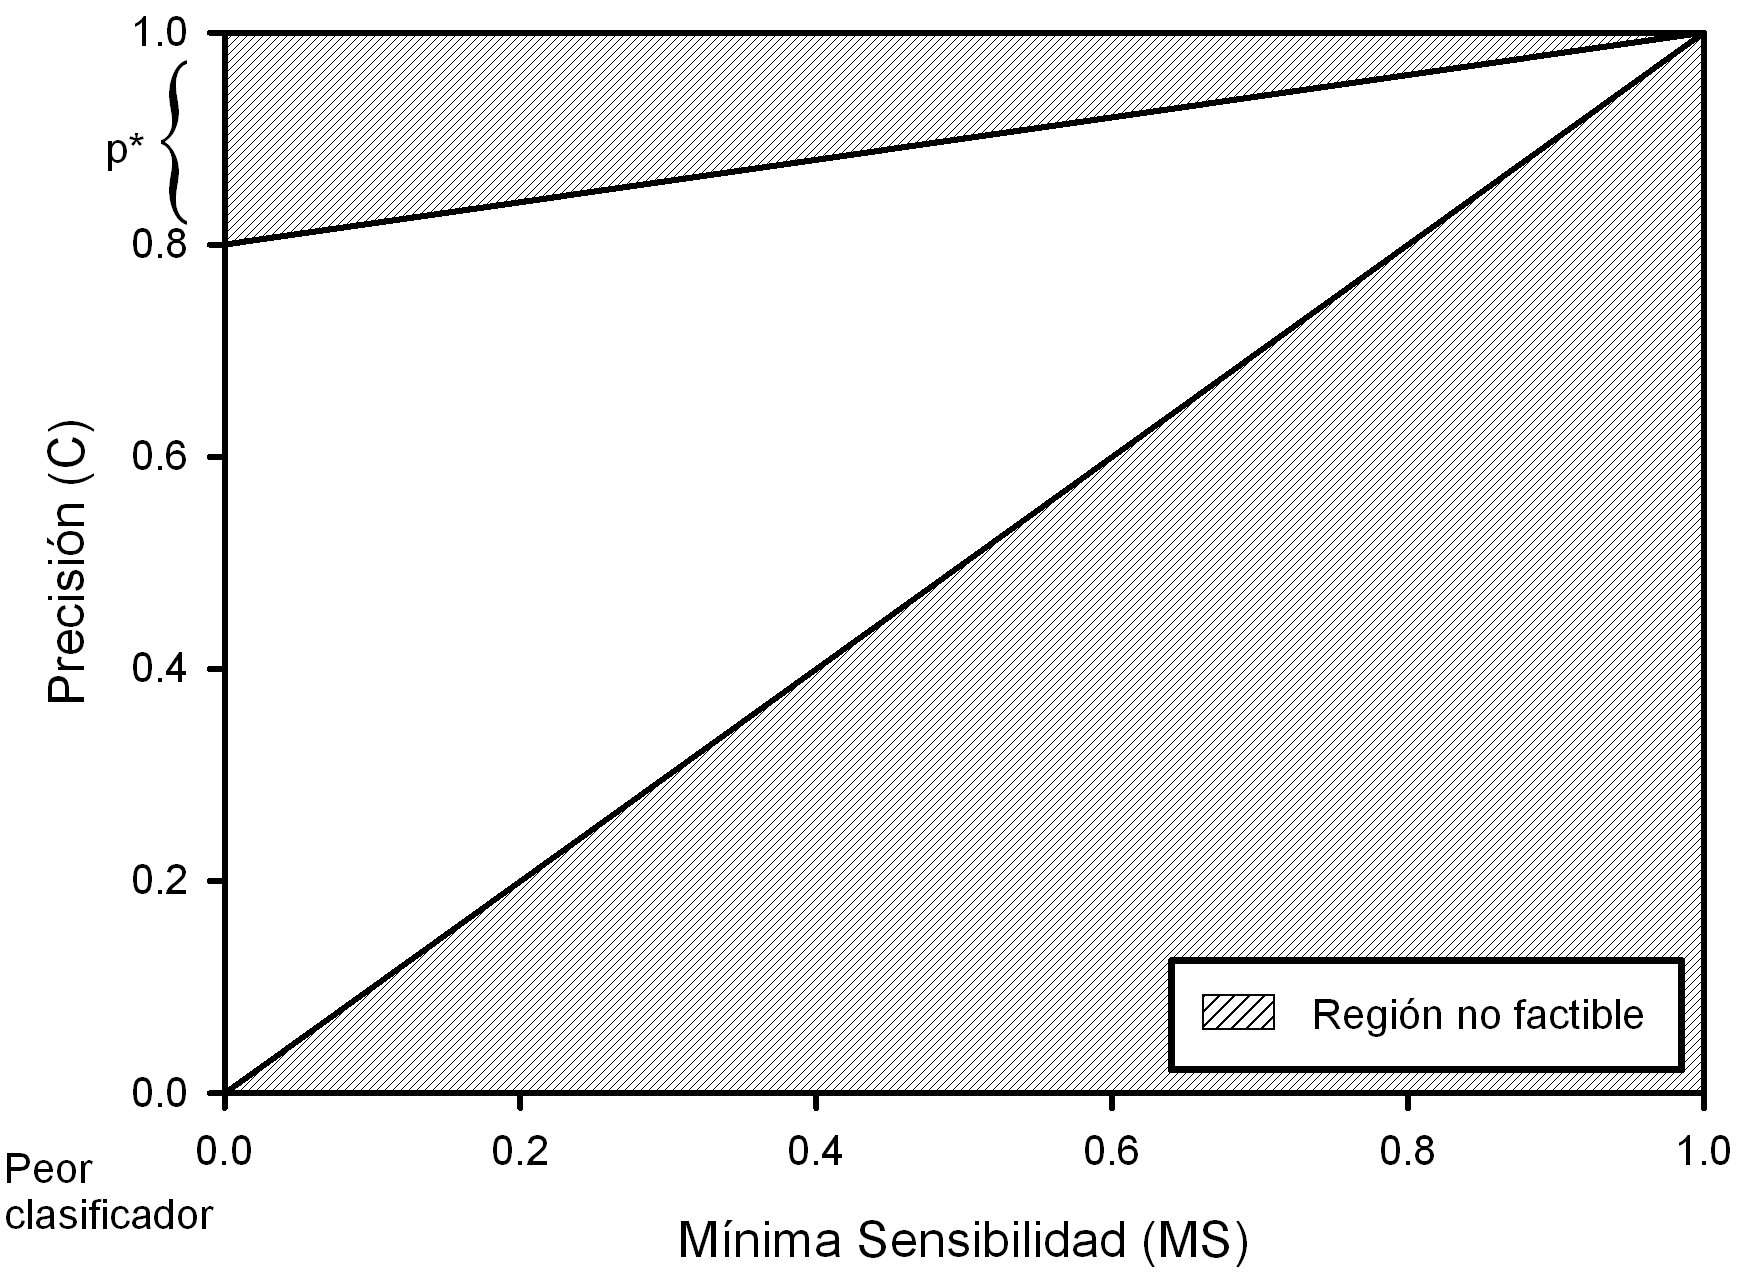
\includegraphics[keepaspectratio,width=11cm]{figuras/regionFactible.jpg}
\caption{Región no factible en el plano $\left(MS,C\right)$ para un
problema de clasificación con $p^*=0.2$.}
\label{regionFactible}
\end{figure}

Obsérvese que un incremento en $C$, no implica necesariamente un incremento
en $MS$. Recíprocamente, un incremento en la $MS$ no significa un
incremento en $C$. Por otro lado, es necesario decir que para un determinado
valor de $C$, un clasificador será mejor cuando se acerque a un punto lo más cercano
posible a la diagonal de la figura \ref{regionFactible} (tanto $C$ como $MS$ toman valores en el
intervalo
$\left[0,1\right]$). Si se utilizan MOEAs como metodología para
la obtención de clasificadores, al comienzo del proceso evolutivo, $MS$ y $C$ pueden ser
cooperativas, e incluso estar lineal y correladas positivamente, pero después de un
determinado número de generaciones, estos objetivos
llegan a ser competitivos, es decir, una mejora en uno de ellos, en general supone un
empeoramiento en el otro. En la Figura \ref{CvsS} se puede ver un ejemplo en el que $MS$ y
$C$ son, en general, objetivos en conflicto, ya que para aumentar el valor de $MS$ en el
clasificador $g_{1}$ es necesario ''perder`` la clasificación de algunos patrones, de
manera que $C$ disminuye en $g_{2}$.
\begin{figure}[htb]
\centering
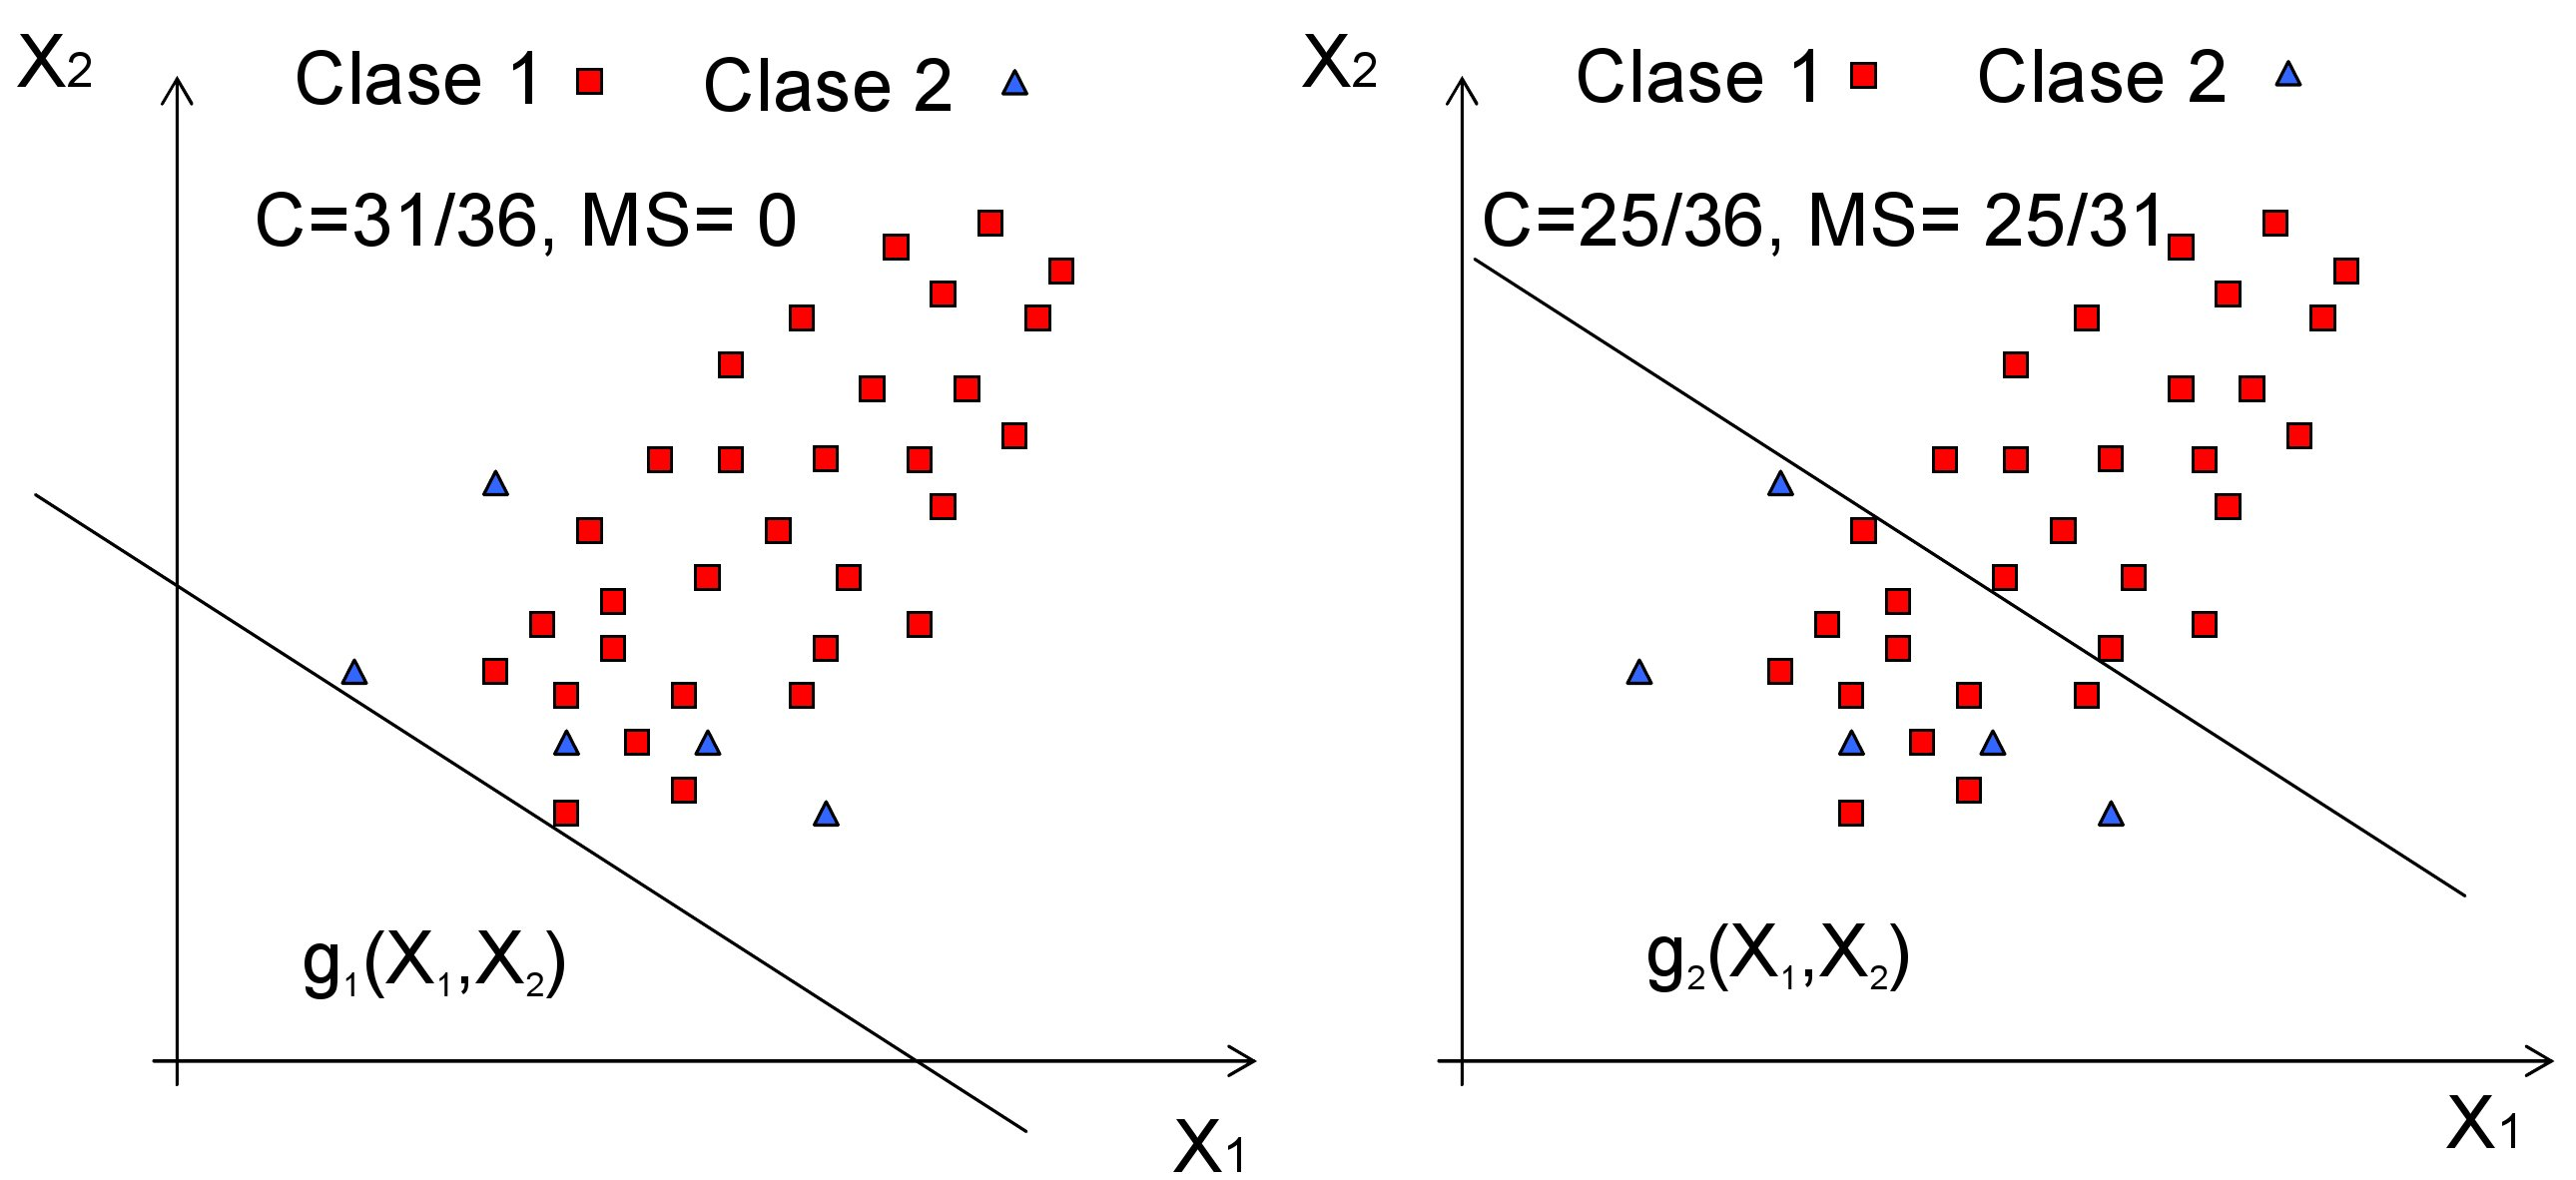
\includegraphics[keepaspectratio,width=12.5cm]{figuras/CvsS.jpg}
\caption{Ejemplo gráfico para describir $MS$ y $C$ como objetivos en
conflicto.}
\label{CvsS}
\end{figure}

A continuación se muestran las propiedades de las medidas $(MS,C)$ como medidas de rendimiento de
un clasificador:
\begin{description}
\item[\textbf{Proposición 1.}] Consideremos de nuevo un problema de clasificación con $Q$
clases, y $J$ la clase con la mínima probabilidad de pertenencia o $p^{*}$, es
decir, $p^{*}=\frac{n_{J\circ}}{N}$, siendo $n_{J\circ}$ el tamaño de la clase
más pequeña y $N$ el tamaño del conjunto de datos. Esta consideración da lugar a la
siguiente desigualdad $MS\leq C\leq 1- \left(1-MS \right) p^{*}$.
\item[\textbf{Demostración.}] Comenzamos demostrando el límite superior de la
inecuación. Teniendo en cuenta
las definiciones de $C$ y $MS$, y que $\displaystyle \sum_{i=1}^Q n_{i\circ}=N$ se puede
comprobar que:
\begin{eqnarray}\label{desigualdad1}
C=\sum_{i=1}^Q \frac{n_{ii}}{n_{i\circ}}\frac{n_{i\circ}}{N}=\sum_{i=1}^Q
S_{i}\frac{n_{i\circ}}{N}=;MS\frac{n_{J\circ}}{N}+\sum_{i\neq
J}S_{i}\frac{n_{i\circ}}{N}\leq\\
\leq MS\frac{n_{J\circ}}{N}+\sum_{i\neq
J}\frac{n_{i\circ}}{N}=MS\frac{n_{J\circ}}{N}+1-\frac{n_{J\circ}}{N}
=1-\left(1-MS\right)\frac{n_{J\circ}}{N}
\nonumber
\end{eqnarray}
Por otro lado, el límite inferior se obtiene de la siguiente forma:
\begin{equation}\label{desigualdad2}
C=\frac{1}{N}\sum_{i=1}^Q n_{ii}=\sum_{i=1}^Q
\frac{n_{ii}}{n_{i\circ}}\frac{n_{i\circ}}{N}=\sum_{i=1}^Q S_{i}\frac{n_{i\circ}}{N}\geq
MS\sum_{i=1}^Q\frac{n_{i\circ}}{N}=MS
\end{equation}
uniendo (\ref{desigualdad1}) y (\ref{desigualdad2}) se puede concluir que
\begin{equation}\label{desigualdad3}
MS\leq C\leq	1-\left(1-MS\right) p^{*}
\end{equation}
% La relación entre $C$ y $MS$ se puede ver en la figura \ref{regionFactible}, de la
% cual se hablará más detalladamente en la sección \ref{seccionfactible}.
\item[\textbf{Proposición 2.}] Sea un problema de clasificación con $Q$ clases y $p^*$ la
mínima de las frecuencias relativas de clase calculadas ''a priori``. Cada punto $(MS,C)$
perteneciente al subconjunto
\begin{displaymath}
		F=\left\lbrace 	(MS,C):0\leq MS\leq 1, MS\leq C\leq 1-p^*+(MS)p^*\right\rbrace
\end{displaymath}
corresponde al menos a un clasificador $g$. Así, el subconjunto completo $F$ es
factible.
\item[\textbf{Demostración.}] Para probar que el subconjunto $F$ es factible,
probaremos que cada punto de dicho subconjunto se puede obtener a partir de una matriz de
confusión. Sea $\left( MS_{0},C_{0}\right)$ un punto en $F$, la demostración se basa en
la construcción de una matriz de confusión con $MS=MS_{0}$ y $C=C_{0}$ para ese punto.
Definamos la función continua y lineal $f:\left[ MS_{0},1\right]
\rightarrow\mathbb{R}$ como:
\begin{displaymath}
f(MS)=(MS_{0})p^*+MS(1-p^*)
\end{displaymath}
la cual satisface
\begin{displaymath}
f(MS_{0})=MS_{0}\leq C_{0}, f(1)=1-p^*+(MS_{0})p^*\geq C_{0}
\end{displaymath}

La continuidad de la función $f$ implica que existe un valor $MS^*\in \left[
MS_{0},1\right]$ de manera que $f(S^*)=C_{0}$. Definamos la siguiente matriz de
confusión:
\setlength{\arraycolsep}{0.75pt}
\renewcommand{\arraystretch}{1.75}
\scriptsize
\[\begin{array}{ccccccccc}
Clase &  & 1 & 2 & \cdots & Q-1 & Q &  &  \\
1 & \multirow{5}{*}{$\left(
\begin{array}{c}
\\
\\
\\
\\
\\
\end{array}\right.$} & (MS_{0})p^* &
(1-MS_{0})p^* & \cdots & \cdots & 0 & \multirow{5}{*}{$\left.
\begin{array}{c}
\\
\\
\\
\\
\\
\end{array}\right)$} & p^* \\
2 &  & \frac{(1-S^*)(1-p^*)}{Q-1} & \frac{S^*(1-p^*)}{Q-1} & \cdots & \cdots & 0 &  &
\frac{1-p^*}{Q-1}\\
\cdots &  & \cdots & \cdots & \cdots & \cdots & \cdots &  & \cdots\\
Q-1 &  & 0 & 0 & \frac{(1-S^*)(1-p^*)}{Q-1} & \frac{S^*(1-p^*)}{Q-1} & 0 &  & \cdots\\
Q &  & 0 & 0 & \cdots & \frac{(1-S^*)(1-p^*)}{Q-1} & \frac{S^*(1-p^*)}{Q-1} &  &
\frac{1-p^*}{Q-1}
\end{array}\]
% Reestrabelcemos de nuevo los tamaños por defecto
\normalsize
\renewcommand{\arraystretch}{1}
\setlength{\arraycolsep}{1pt}
\newline

Se puede observar que las sensibilidades cumplen lo siguiente:
\begin{displaymath}
S_{1}=S_{0}, S_{2}=...=S_{Q}=\frac{S^*(1-p^*)}{Q-1}
\frac{Q-1}{1-p^*}=S^*
\end{displaymath}

Por tanto $\displaystyle
MS=min\left\lbrace MS_{0},S^*\right\rbrace=MS_{0}$, ya que $\displaystyle S^*\in\left[
MS_{0},1\right]$. Por otra parte, se verifica que la precisión, $C$, asociada a la matriz
es:
\begin{displaymath}
C=MS_{0}p^*+(Q-1)S^* \frac{1-p^*}{Q-1}=f(S^*)=C_{0}
\end{displaymath}
Finalmente, a partir de la condición $\displaystyle p^*\leq \frac{1}{Q}$ obtenemos que
\begin{displaymath}
p^*Q\leq1 \Longrightarrow p^*Q-p^*\leq 1-p^*\Longrightarrow p^*\leq \frac{1-p^*}{Q-1}
\end{displaymath}
y podemos concluir que la mínima probabilidad de las columnas es $p^*$.
\item[\textbf{Proposición 3.}] El área $A$ del conjunto factible $F$ (región dibujada en
blanco en la figura \ref{regionFactible}) verifica que $\displaystyle A= \frac{1-p^*}{2}$,
donde $p^*$
es la mínima de las frecuencias relativas de cada clase.
\item[\textbf{Demostración.}] La demostración es inmediata a partir de la Proposición 2.
Cuando el número de clases aumenta o el problema es altamente desbalanceado, el valor de
$\displaystyle p^*\leq \frac{1}{Q}$ disminuye en ambos casos. Por tanto una consecuencia
de la Proposición 3 es que, el área de $F$ aumenta cuando el nivel de desbalanceo o el
número de clases aumenta. Un análisis similar prueba que el valor mínimo del área se
alcanza cuando el problema es totalmente balanceado, es decir, $\displaystyle p^*=
\frac{1}{Q}$. En consecuencia, en problemas no balanceados, la línea que define el borde
superior del conjunto en el plano $(MS,C)$
tiende a ser horizontal, y el rango de valores de $MS$ será mayor incluso para valores
altos de $C$. En este caso, el valor de $C$ como medida única de un clasificador
multiclase es insuficiente, ya que esconde muchas posibilidades diferentes para $MS$.
Estos comentarios muestran que las medidas $(MS,C)$ pueden ser especialmente ventajosas
en problemas con cierto desbalanceo o cuando el número de clases es alto, confirmando
que, por si sola, la medida $C$ es inadecuada en estas situaciones.

Finalmente, analizamos la relación existente entre las medidas $(MS,C)$ y las curvas
ROC en problemas binarios. Los siguientes resultados establecen la relación
entre los dos espacios en un problema de clasificación binario, probando que no hay
equivalencia entre ellos. En este sentido las medidas $(MS,C)$ constituyen un punto de vista
complementario a las curvas ROC en problemas binarios.
\item[\textbf{Proposición 4.}] Sea $Q=2$ el número de clases y $q$ la probabilidad ''a
priori`` de que un patrón pertenezca a la primera clase. Entonces cada punto
$(TPR_{0},FPR_{0})$ en el plano \textit{ROC} determina un único punto factible
$(MS_{0},C_{0})$ en el plano $(MS,C)$ definido por:
\begin{displaymath}
MS_{0}	=min\left\lbrace TPR_{0}, 1-FPR_{0}\right\rbrace \qquad
C_{0}=TPR_{0}q+(1-FPR_{0})(1-q)
\end{displaymath}
Inversamente, cada punto $(MS_{0},C_{0})$ de $F$, determina dos puntos en el plano
\textit{ROC} dado por:
\begin{align}
	FPR_{1}&=\frac{1-C_{0}-(1-MS_{0})q}{1-q},\qquad TPR_{1}=MS_{0} \nonumber \\
	FPR_{2}&=1-MS_{0}, \qquad TPR_{2}=\frac{C_{0}-MS_{0}(1-q)}{q} \nonumber
\end{align}
\item[\textbf{Demostración.}] Sea $\displaystyle (TPR_{0},FPR_{0})$ un punto en el
plano ROC, supongamos que la matriz de confusión está dada por $\left( \begin{array}{cc}
n_{11} & n_{12}\\
n_{21} & n_{22}
\end{array}\right) $, y sea $N$ el número de patrones. Recordando la definición de
MS, tenemos que
\begin{equation}\label{p4-1}
S_{0}=min\left\lbrace TPR_{0}, 1-FPR_{0}\right\rbrace
\end{equation}
Por otro lado, la precisión $C_{0}$ es $\displaystyle \frac{n_{11}}{N}+\frac{n_{22}}{N}$.
Teniendo
en cuenta que $\displaystyle TPR_{0}=\frac{n_{11}}{n_{1\circ}}$ y
$FPR_{0}=\frac{n_{21}}{n_{2\circ}}$, donde $n_{1\circ}=n_{11}+n_{12}$ y
$n_{2\circ}=n_{21}+n_{22}$ son
el número de patrones en la primera y segunda clase respectivamente, y que $q$ es la
probabilidad "a priori" de la primera clase, tenemos
\begin{equation}\label{p4-2}
\begin{split}
C_{0}&=\frac{n_{11}}{N}+\frac{n_{22}}{N}=\frac{n_{11}}{n_{1\circ}}\frac{n_{1\circ}}{N}
+\frac{n_ {22}}
{n_{2\circ}}\frac{n_{2\circ}}{N}= \\
&=(TPR_{0})q+(TPR_{0})(1-q)=(TPR_{0})q+(1-FPR_{0})(1-q)
\end{split}
\end{equation}
Inversamente, si $(MS,C)$ es un punto factible, a partir de las ecuaciones \ref{p4-1} y
\ref{p4-2} previamente establecidas se tiene que
\begin{align}
FPR_{1}&=\frac{1-C_{0}-(1-S_{0})q}{1-q},\qquad TPR_{1}=S_{0} \nonumber \\
FPR_{2}&=1-S_{0}, \qquad TPR_{2}=\frac{C_{0}-S_{0}(1-q)}{q} \nonumber
\end{align}
dependen estos puntos de la clase en la que la sensibilidad alcance el valor más bajo.
Obsérvese que $0\leq TPR_{0},FPR_{0}\leq1$.
A partir de estos resultados podemos hacer las siguientes observaciones:
\begin{enumerate}
	\item Es fácil probar que
	\begin{displaymath}
	FPR_{2}=FPR_{1}+\frac{C-SM}{1-q}, \qquad TPR_{2}=TPR_{1}+\frac{C-MS}{q}
	\end{displaymath}
	siendo la pendiente del segmento que une los puntos ROC asociados el
	$\displaystyle \left(\frac {1-q}{1}\right) $ por ciento entre las probabilidades ''a
priori``,
	independientemente del punto $(MS_{0},C_{0})$ considerado. Como $\displaystyle
	\left( \frac{1-q}{1}>0\right)$, ningún punto domina a los demás.
	\item Los puntos obtenidos en el plano ROC son iguales, si y solo si, $MS=C$.
	Es decir, los puntos en la diagonal del plano $(MS,C)$ determinan solamente un punto en
el
	plano ROC.
\end{enumerate}
\end{description}

\section{Problemas no balanceados y/o con gran número de clases}\label{balanceados}
\noindent Como ya hemos comentado en la sección anterior, cuando el número de clases
aumenta, o cuando existe un problema altamente
desbalanceado, el valor de $\displaystyle p^*=\frac{n_{\circ j}}{N}\leq \frac{1}{Q}$ disminuye, y la
línea
del borde superior de la región factible, dentro del plano $\left(MS,C\right)$, tiende a
ser horizontal, es decir, a tomar el valor $C=1$, de manera que el rango de valores de
$MS$ será más amplio cuando $C$ tome valores altos. En este tipo de problemas
\cite{Ho2002,Murphey2004} es difícil
mantener un nivel de precisión alto en cada clase,	debido a la dificultad en el
aprendizaje a partir de clases con pocos patrones, que puede conllevar una disminución
del valor de $C$ en el conjunto de generalización.

De forma general, la solución aportada al tratamiento de problemas no balanceados se
puede dividir en aproximaciones a nivel de datos y aproximaciones a nivel de algoritmo
\cite{He2009,Sun2009}.

\begin{itemize}
\item A nivel de datos, la solución es rebalancear la distribución por clase mediante
técnicas
de remuestreo, ya sea quitando patrones de la clase mayoritaria o incluyéndolos en la
minoritaria, o incluso una combinación de las dos \cite{Kubat97,Chawla2002}. Estos métodos
conllevan desventajas:
\begin{enumerate}
\item La distribución óptima por clase de un conjunto de entrenamiento es usualmente
desconocida.
\item Una estrategia de remuestreo poco efectiva
puede ocasionar riesgos de pérdida de información sobre las clases mayoritarias en caso de
hacer un muestreo eliminando patrones, o sobre las clases minoritarias, en caso de hacer
un muestreo aumentando el numero de patrones, pudiendo en este último caso ocasionar un
sobreajuste o sobreaprendizaje de los datos.
\item En la mayoría de los casos existe un inevitable coste extra relacionado con el
análisis y procesamiento de los datos.
\end{enumerate}
\item A nivel algorítmico, lo que se hace es adaptar el aprendizaje del algoritmo
para que influya sobre la clase minoritaria \cite{Jankowski2001b}. En \cite{Fernandez2009}
y \cite{Fernandez2009a} se pretende que dos EAs para ANNs vayan
nivelando el porcentaje de buena clasificación en cada una de las clases de un
problema determinado, o al menos dejarlas de la manera más equilibrada posible, usando
respectivamente $MS$ y el coeficiente de variación de las sensibilidades de
todas las clases. En \cite{Martinez-Estudillo2008} este objetivo se aborda utilizando un
algoritmo en dos etapas, optimizando $C$ en la primera etapa, y en la segunda optimizando
una función definida a partir de $C$ y $MS$, que geométricamente corresponde al área de un
recinto definido por el clasificador en la región factible de la figura
\ref{regionFactibleAreaEA}, donde dicha área viene definida por:
\begin{displaymath}
A(MS,C)=(1-MS)(1-C)-\frac{1}{2}\left[ (1-C)^2-p^*(1-MS)^2\right]
\end{displaymath}
\end{itemize}

La mayoría de nuevos métodos que se describen en esta tesis doctoral para la obtención de
clasificadores usando las medidas $(MS,C)$ son métodos a nivel de algoritmo, y bajo este
punto
de vista, $MS$ y $C$ pueden ser ventajosas como medidas de precisión en problemas no
balanceados y/o con un número de clases elevado.
\newpage

\begin{figure}[!htp]
\centering
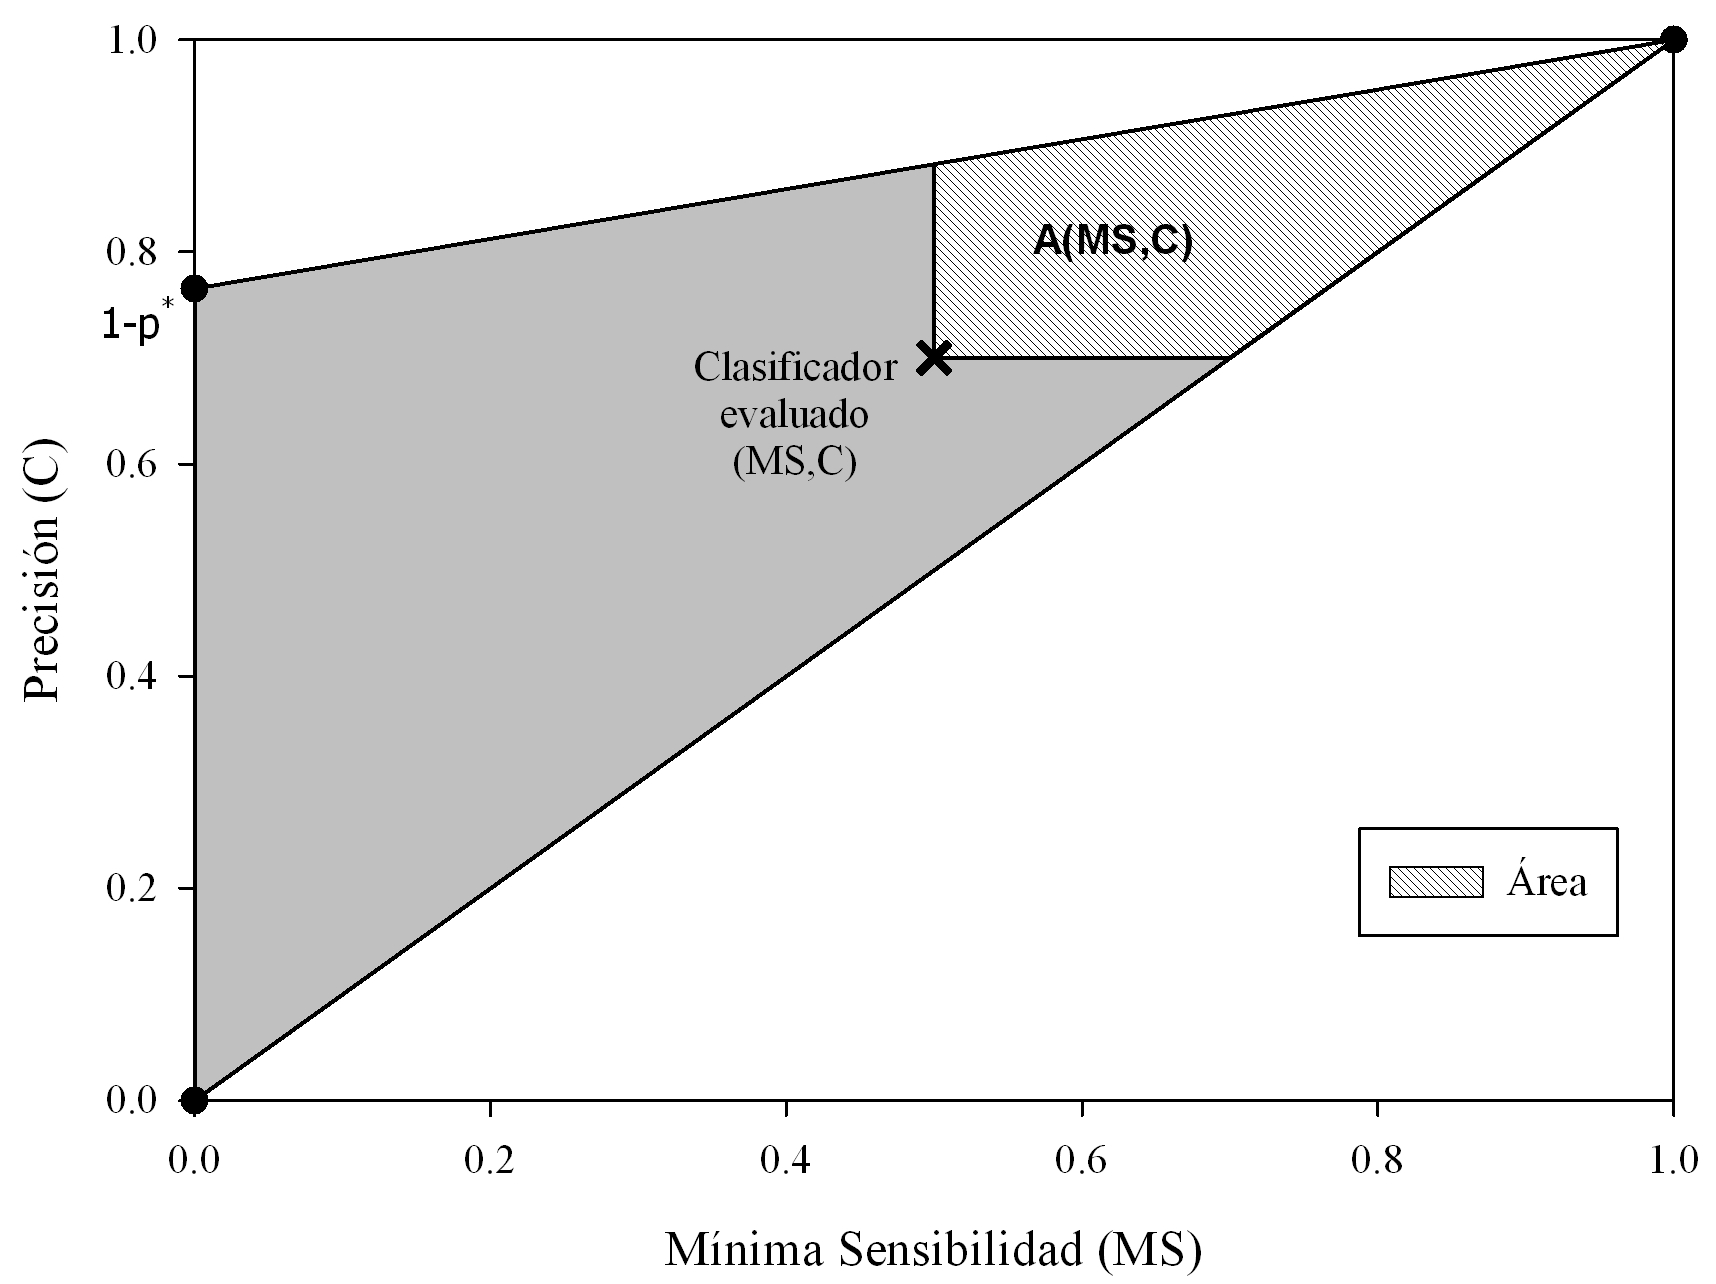
\includegraphics[keepaspectratio,width=9cm]{figuras/EA.jpg}
\caption{Área sobre un clasificador evaluado, función $A(MS,C)$.}
\label{regionFactibleAreaEA}
\end{figure}
\paginavaciacompleta
		%\paginavaciacompleta
		% \chapter{Redes neuronales artificiales}\label{redesneuronales}
% \begin{quotation}
% \begin{small}
% \textit{La vergüenza de confesar el primer error hace cometer otros muchos.}
% \end{small}
% \begin{flushright}Jean de la Fontaine.\end{flushright}
% \end{quotation}
\section{Modelos de redes neuronales artificiales}\label{modelos}
\noindent
% Las ANNs \cite{Bishop1995,Haykin2008} se pueden definir como estructuras que se
% diseñan para resolver cierto tipo de problemas asociados a emular la forma en la que el
% cerebro humano puede resolverlos, de esta manera  su  interpretación  biológica  es
% similar a la activación  de  las neuronas cerebrales.  A diferencia  de  los
% algoritmos procedurales convencionales que  siguen  un  flujo secuencial,  las
% computaciones neuronales se realizan a través de un gran número de nodos.
Una  ANN \cite{Bishop1995,Haykin2008} es un  modelo matemático que simula un sistema
neuronal biológico, donde las neuronas se modelan mediante unidades
de  procesamiento  o  nodos interconectados.  Cada  unidad  de  procesamiento  se
compone de un conjunto de conexiones  de  entrada,  una  función  de  propagación
(encargada  de  computar  la entrada  total combinada de todas las conexiones), un núcleo
central de proceso (encargado de aplicar la función de activación) y una salida (por donde
se transmite el valor de activación a otras unidades). De esta forma, los elementos que
caracterizan un nodo de una
ANN son:
\begin{description}
	\item[Conexiones ponderadas:] Hacen  el  papel  de  las conexiones  sinápticas.  La
	existencia  de conexiones determina si es posible que un nodo influya sobre otro,
	mientras que el valor de los pesos y el signo de los mismos definen el tipo
	(excitativo/inhibitorio) y la intensidad de la influencia.
	\item[Función de activación:] Calcula el valor de base o entrada total al nodo,
	generalmente como una  suma  ponderada  de  todas  las  entradas  recibidas,  es
	decir,  de  las entradas multiplicadas por  el  peso  o  valor  de  las  conexiones.
	\item[Función de salida o de transferencia:] Calcula la salida del nodo en función de
	la activación de la misma. Se  usan diferentes	tipos  de  funciones,  desde  simples
	funciones de umbral a funciones no lineales.
 \end{description}

La  arquitectura  de  una  ANN (véase figura \ref{redSigmoideHaciaDelante}) es  la manera
en que se disponen sus nodos y conexiones. Los nodos según  su situación  dentro  de  la
red pueden
ser  de  tres  tipos:
\begin{description}
	\item[Nodos  de entrada:] Reciben  las  señales  de entrada de la red, es decir, los
	valores de las variables independientes del modelo, y forman la capa	de entrada.
	\item[Nodos de salida:] Envían las señales de salida al exterior, es decir, los
	valores de las variables dependientes del modelo, y forman la capa de salida.
	\item[Nodos ocultos:] Son el resto de nodos,  y  se  agrupan  en  una  o  más  capas
	ocultas. Normalmente se suelen utilizar ANNs con una sola capa oculta, aunque puede
	haber varias.
\end{description}

\begin{figure}[htb]
\centering
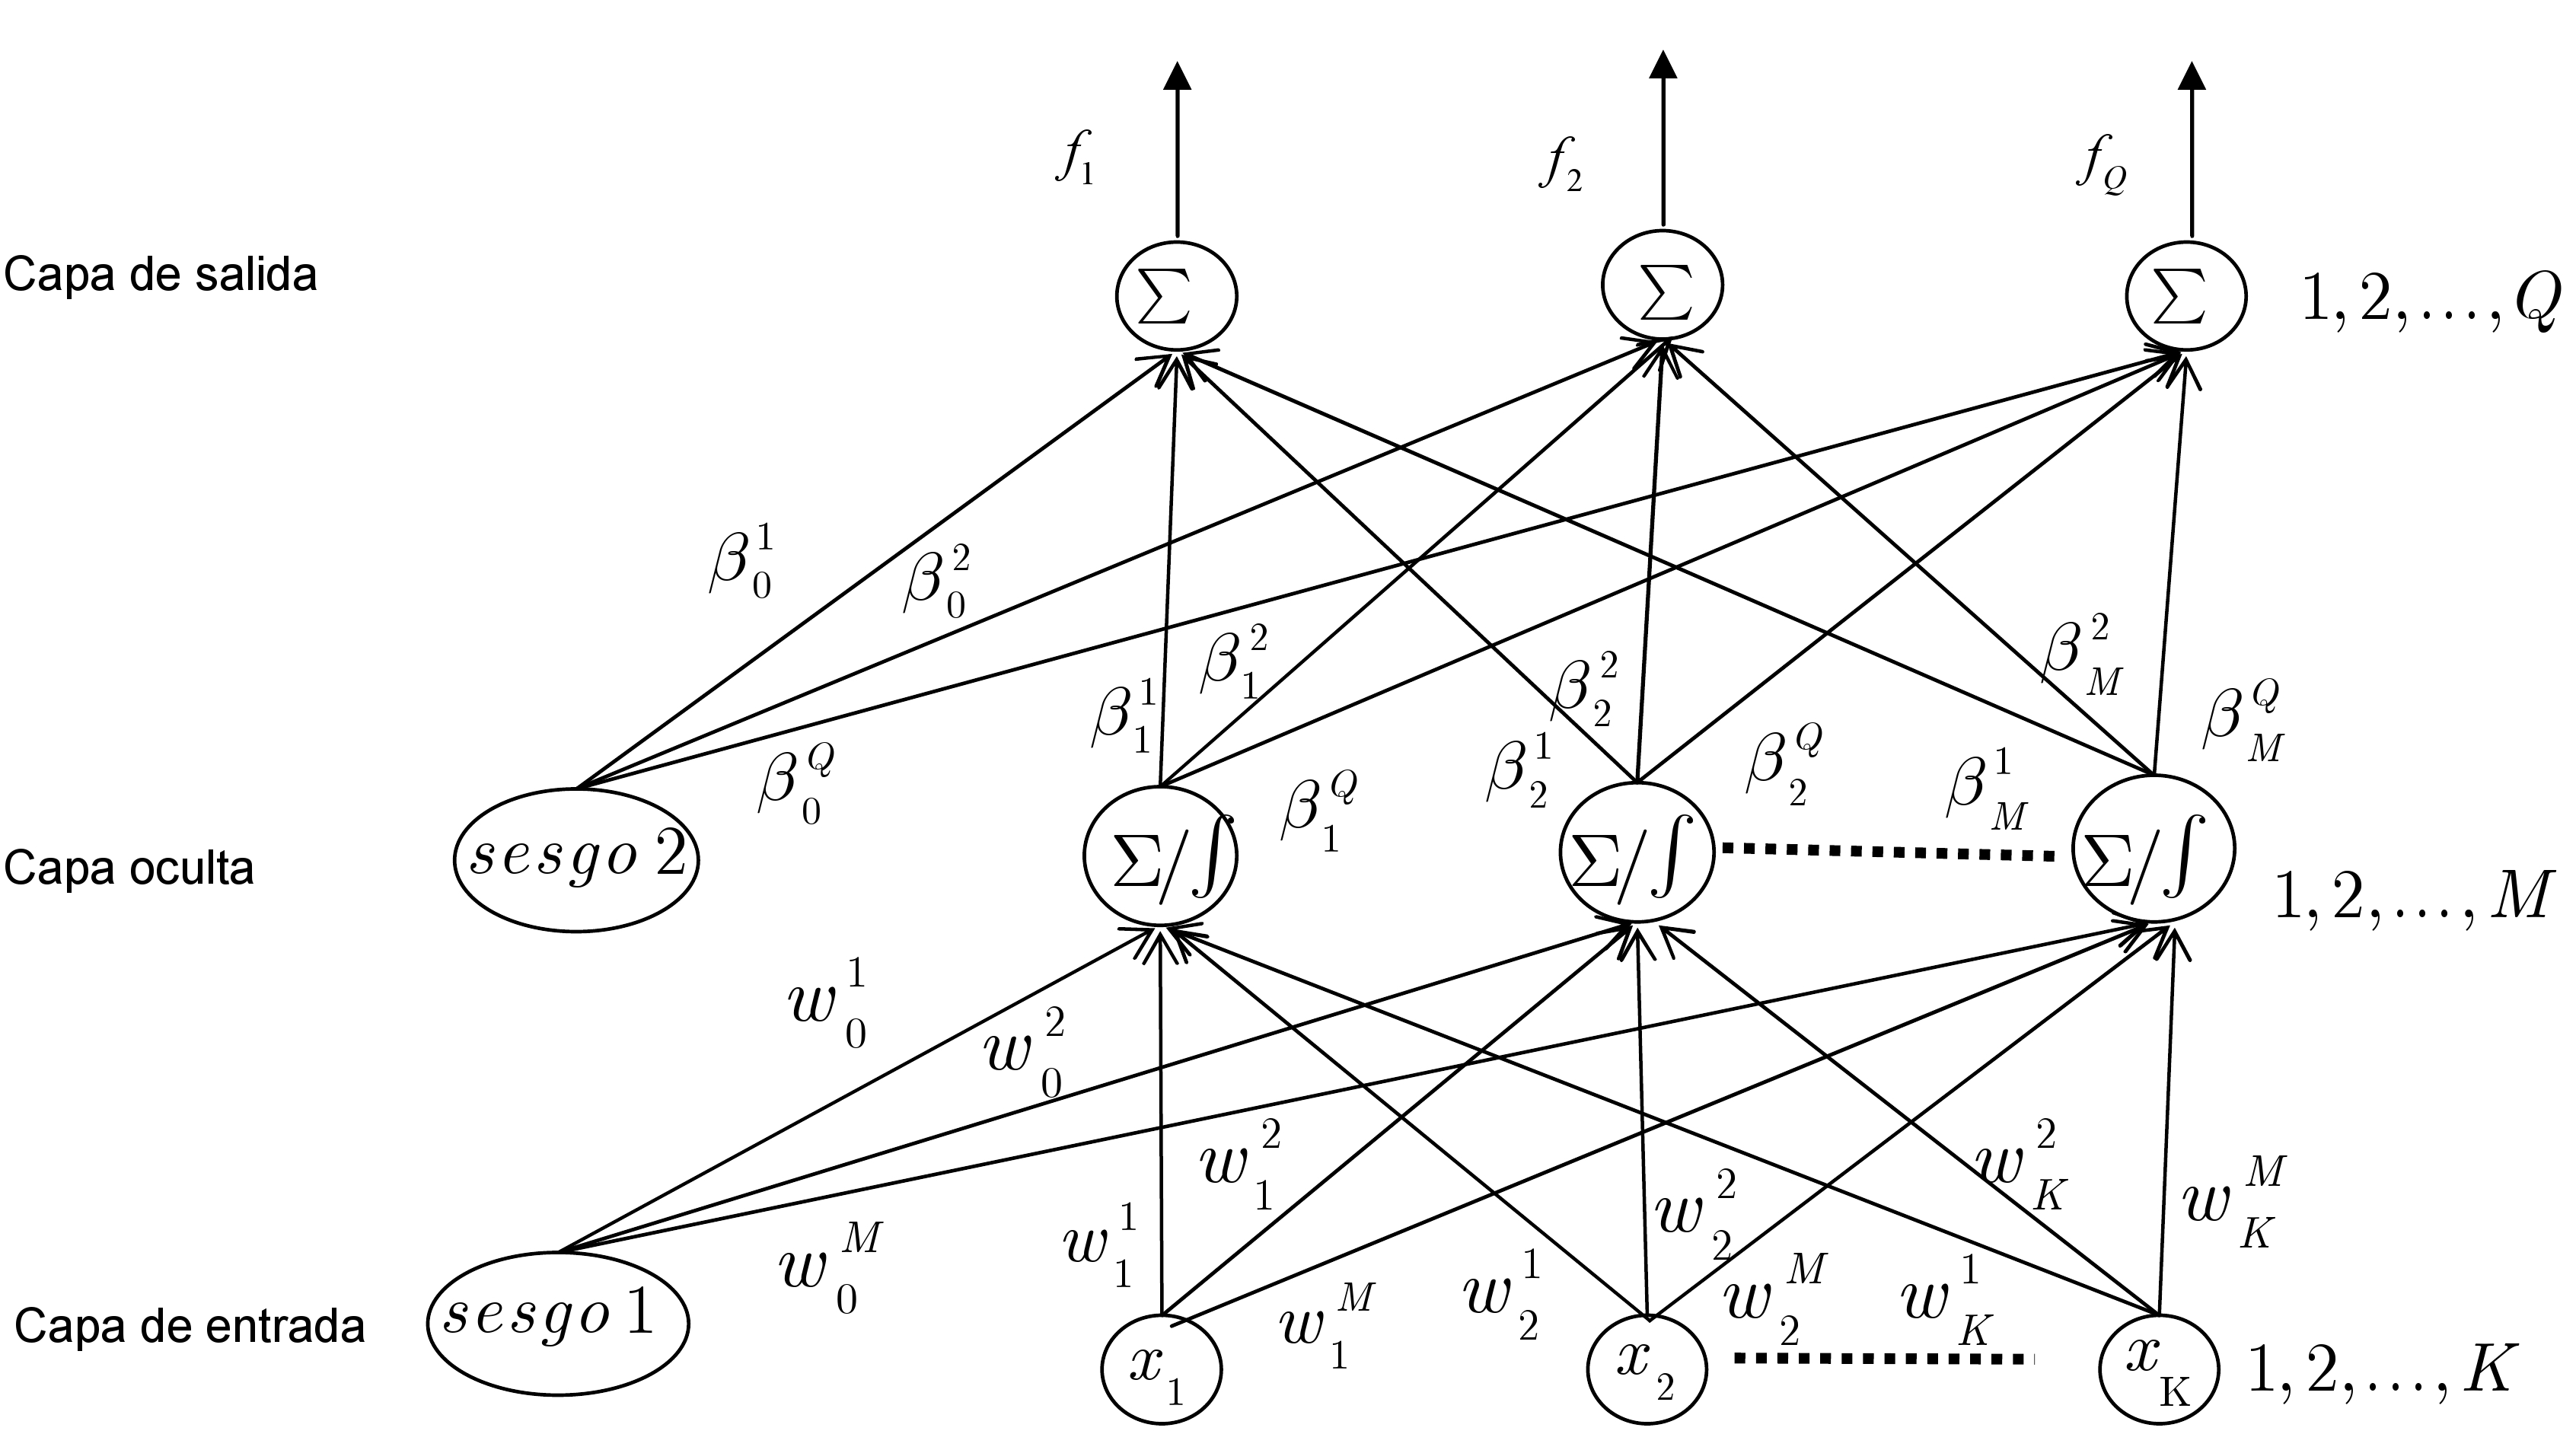
\includegraphics[keepaspectratio,width=12.5cm]{figuras/redSigmoideHaciaDelante.jpg}
\caption{Red neuronal hacia delante con unidades de base sigmoide y una capa oculta.}
\label{redSigmoideHaciaDelante}
\end{figure}

Existen  distintas  formas  de transmisión  de  la información entre los nodos de una ANN,
que determinan la naturaleza de la misma. De este modo, los tipos de transmisión son los
siguientes:
\begin{description}
	\item[Transmisión hacia delante:] Este  tipo  de transmisión  se
	produce desde los nodos de la capa de entrada	hasta los	nodos de la capa de salida.
	Las ANNs que presentan este tipo de transmisión	se
	denominan redes de transmisión hacia	delante o \textit{feedforward}.
	\item[Transmisión lateral:] Este tipo de transmisión se produce	entre nodos
	de la 	misma capa. Las	ANNs que presentan este tipo de transmisión se denominan
	redes con	transmisión lateral.
	\item[Transmisión hacia atrás:] Este tipo de transmisión	(también llamada transmisión
	\textit{feedback}) se	produce desde los nodos de la capa de salida hasta los nodos de
	la capa de entrada. Las	ANNs	que  presentan  este  tipo  de  transmisión  se
	denominan  redes  con  realimentación o redes recurrentes.
 \end{description}
En este trabajo trabajo se utilizan redes de transmisión hacia delante, con una sola
capa oculta y con unidades de base sigmoide, por su buena adaptación y resultados en
problemas de clasificación de patrones.

El modelo funcional o función de salida asociada a cada
una de las neuronas de la salida de este tipo de redes es el siguiente:
\begin{equation}\label{modelof}
	f_{q}\left(\mathbf{x},\mathbf{\Theta}_{q} \right)= \beta_{0}^q + \sum_{j=1}^M
	\beta_{j}^q B_{j} \left( \mathbf{x},\mathbf{w}_{j}\right), \quad \text{para } q=1...Q
\end{equation}
donde $Q$ es la neurona de salida $q$ de la
red (en el caso de que haya varias salidas), $\displaystyle
\mathbf{\Theta}_{q}=\left(\beta_{0}^q,\beta_{1}^q,...,\beta_{M}^q,
\mathbf{w}_{1},...,\mathbf{w}_{M}\right)$ es el vector de pesos de esa neurona
$q$,
$\displaystyle \mathbf{w}_{j}=\left( w_{0}^j,w_{1}^j,...,w_{k}^j\right) $ es el vector de
pesos de las conexiones entre la capa de entrada y la neurona de la capa oculta $j$, $M$
es el número de neuronas de la capa oculta (ver figura \ref{redSigmoideHaciaDelante}), $K$ el número
de neuronas o características en la capa de entrada (ver figura \ref{redSigmoideHaciaDelante}),
$\mathbf{x}$ el valor de las entradas de la ANN, $\displaystyle B{j}\left(
\mathbf{x},\mathbf{w}_{j}\right)$ es la función de base de la neurona $j$
de la capa oculta y $\displaystyle \beta_{0}^q$ y $\displaystyle w_{0}^j$ son los sesgos
del modelo asociado a la neurona $q$ en la capa de salida, y a la neurona $j$ de la capa
oculta respectivamente.

\section{Taxonomía}\label{taxonomia}
\noindent Se pueden considerar dos tipos fundamentales de funciones de
base o transferencia en una ANN:
\begin{description}
\item[Funciones de ventana:] Son funciones de entorno local, como pueden ser las
funciones de base radial (\textit{Radial  Basis  Functions}, RBFs).  Poseen  una  mayor
capacidad de aproximar  datos anómalos aislados, pero una mayor dificultad en entornos
globales o cuando el número de entradas es demasiado alto.
\item[Funciones de proyección:] Son funciones de entorno global, como las unidades
de base sigmoide (\textit{Sigmoidal Units}, SUs) o las  unidades de base Producto
(\textit{Product	Units}, PUs). Al ser globales, presentan dificultades en 	la
aproximación de  datos	aislados pero suelen actuar mejor en problemas donde el	número
de variables es alto.
\end{description}

En  general,  consideraremos  dos  tipos  de  modelos  de  red, en función de
la activación de las variables independientes: Modelos aditivos  y
modelos multiplicativos:
\begin{description}
	\item[Modelo aditivo:] Este modelo es el más utilizado dentro de las ANNs, y los nodos
	que componen la estructura de la red proporcionarían la siguiente salida:
	\begin{displaymath}
	B{j}\left(
	\mathbf{x},\mathbf{w}_{j}\right)=h\left(w_{0}^j+w_{1}^jx_{1}+w_{2}^jx_{2}+...+w_{n}^jx_{
	 k} \right)
	\end{displaymath}
	siendo $n$ el número de características o neuronas de entrada de la red, $w_{0}^j$ el
	sesgo del modelo asociado a la neurona $j$ y $h(.)$ la función de salida o
transferencia
	de la	neurona $j$.
	\item[Modelo multiplicativo:] Este modelo es más reciente, e   intenta  afrontar
	aquellos  casos  en	los  que  existe  una  interacción  entre  las  variables  y  las
	regiones  de decisión	que no  pueden 	separarse por hiperplanos:
	\begin{displaymath}
	B_{j}\left(\mathbf{x},\mathbf{w}_{j}\right)=
	x_{1}^{w_{1}^j}x_{2}^{w_{2}^j}...x_{n}^{w_{k}^j}
	\end{displaymath}
	Como se puede observar no existe un sesgo, pues carece de sentido para este tipo
	de modelos. La función de salida o transferencia suele ser la función identidad.
\end{description}

\subsection{Redes con unidades de base sigmoides}\label{unidadesSigmoide}
\noindent Las neuronas con SUs tienen la siguiente expresión como
función de salida o transferencia:
\begin{displaymath}
	B_{j}\left(\mathbf{x},\mathbf{w}_{j}\right)=\frac{1}{1+exp\left(-\left(w_{0}
^j+\sum_{i=1}^{K} w_{i}^{j}x_{i} \right) \right)}
\end{displaymath}

En la figura \ref{ejemploSigmoides} se muestran algunos ejemplos de funciones de base
sigmoide.

\begin{figure}[htb]
\centering
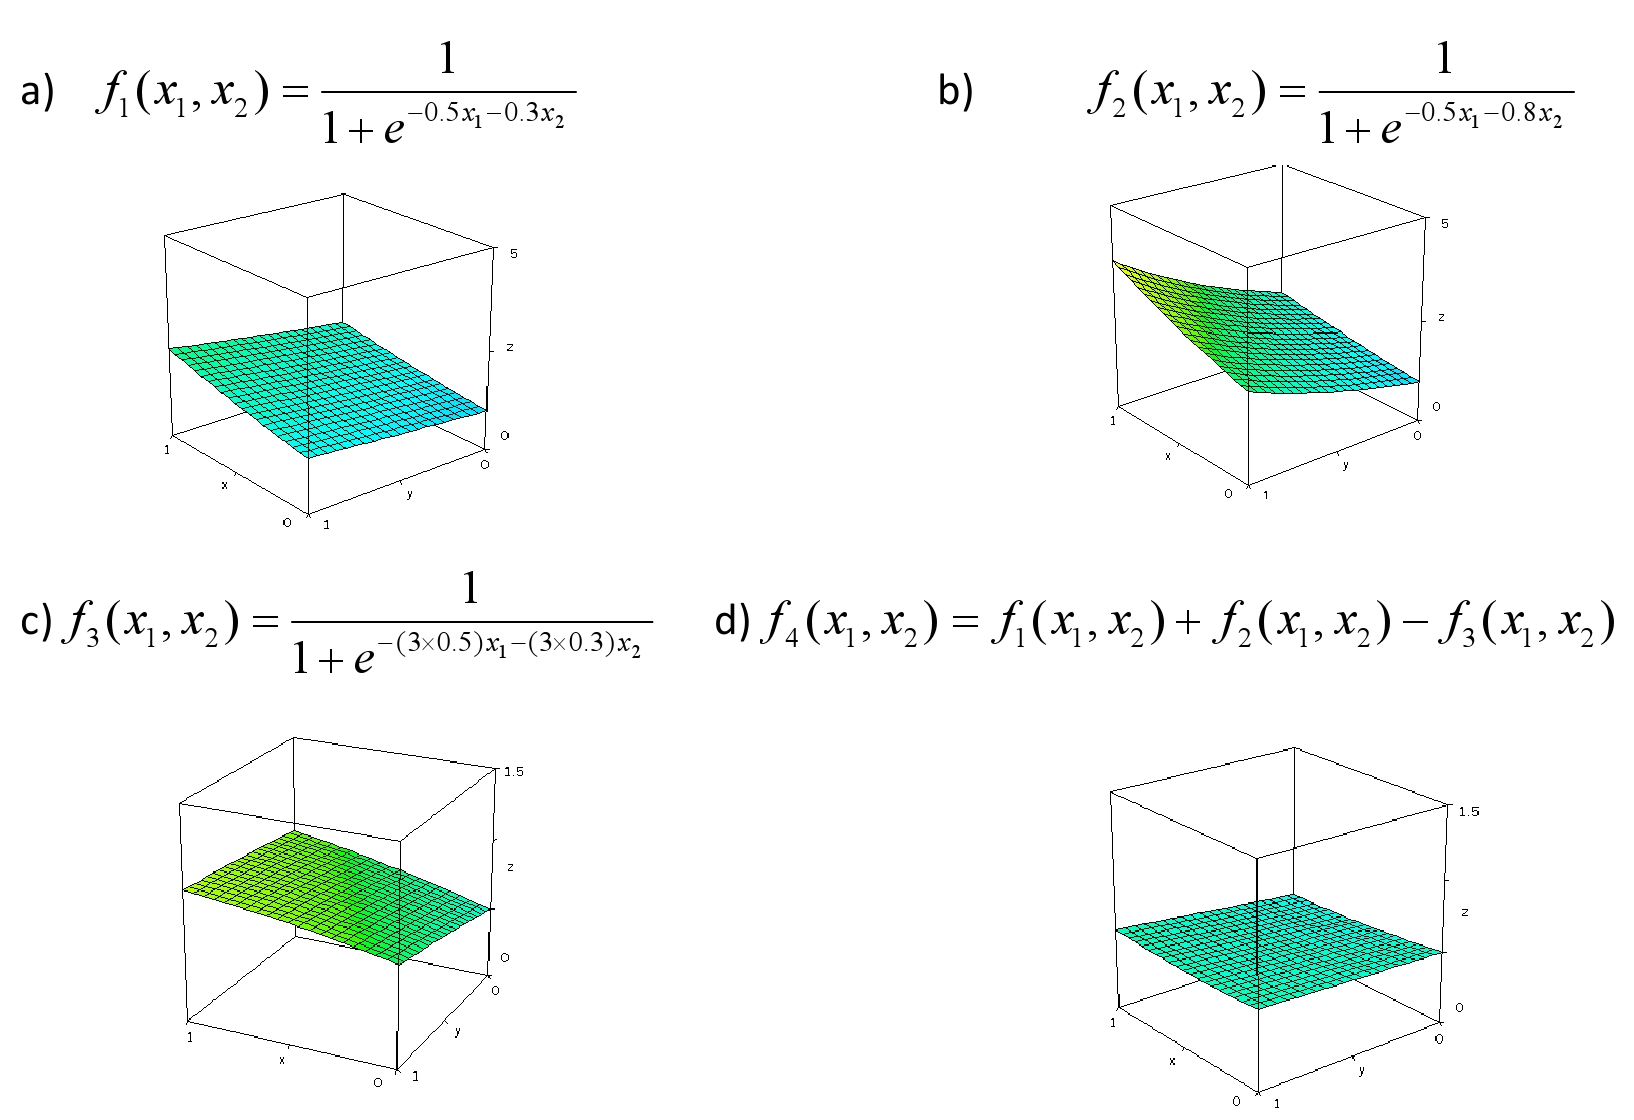
\includegraphics[keepaspectratio,width=12.5cm]{figuras/ejemploSigmoides.jpg}
\caption{Ejemplos de funciones de base sigmoide, SUs.}
\label{ejemploSigmoides}
\end{figure}

Las redes con SUs, también conocidas como perceptrón multicapa (\textit{Multi Layer
Perceptron}, MLP), poseen las siguientes propiedades:
\begin{enumerate}
	\item La familia de funciones reales que representan puede aproximar cualquier función
	continua	con  suficiente  precisión,  con  tal  de  que  el  número  de  nodos  de  la
	capa	oculta  no  esté	acotado. Se dice por tanto que son aproximadores universales.
	\item Son fáciles de entrenar, aunque se obtienen con frecuencia óptimos locales.
	\item Se obtienen modelos eficientes en entornos alisados.
	\item Son funciones acotadas.
	\end{enumerate}
En la figura \ref{redSigmoideHaciaDelante} se representa una ANN hacia delante
con unidades de base sigmoides, con una capa de entrada, una capa oculta y una capa de
salida.

\subsection{Redes con unidades de base producto}
\noindent     Las ANNs con PUs introducidas por Durbin y Rumelhart \cite{Durbin1989} en
1989, son aquellas que están formadas por nodos que siguen un modelo multiplicativo de
proyección, con la siguiente función de salida o transferencia:
\begin{displaymath}
B_{j}\left(\mathbf{x},\mathbf{w}_{j}\right)=x_{1}^{w_{1}^j}x_{2}^{w_{2}^j}...x_{n}^{
	w_{n}^j}=\prod_{i=1}^n x_{i}^{w_{i}^j}
\end{displaymath}

Entre las ventajas de las redes PU se encuentran las siguientes:
\begin{enumerate}
	\item Como consecuencia del Teorema de Stone-Weierstrass \cite{Bishop1961}, se ha
	demostrado que las
	redes PU son aproximadores universales, (obsérvese que las funciones
	polinómicas de varias variables, son un subconjunto de los modelos basados en unidades
	producto).
	\item La  posibilidad  de  usar  exponentes  negativos  permite  expresar  cocientes  y
	entre  las variables.
	\item Durbin  y  Rumelhart \cite{Durbin1989} demostraron  que  la  capacidad  de
	información  de  una
	única unidad  de tipo  producto  (medida  como  la  capacidad  para  el  aprendizaje
	de	patrones booleanos aleatorios) es aproximadamente igual a $3N$, comparado con el
	valor de	$2N$ que corresponde a una unidad de tipo aditivo, siendo $N$ el número de
	entradas de la unidad.
	\item Los  exponentes  del  modelo  son  números  reales.  Esta  característica  tiene
	especial importancia,  sobre  todo  si  se  tiene  en  cuenta  que  son  frecuentes
	las	situaciones  en  el modelado de datos reales en las que, la relación entre las
	variables	responde a una estructura de  tipo  potencial,  donde  las  potencias  no
	están	restringidas  a  los  números naturales  o enteros.
	\item Permiten  implementar  funciones  polinómicas  de  orden  superior.  Han
	demostrado	buenos resultados en el modelado de datos en los que existen interacciones
	de diferentes	órdenes entre  las  variables  independientes  del  problema.  De  esta
	forma,	cuando existen interacciones  entre  las  variables  que  intervienen  en  un
	determinado  fenómeno, las  ANNs basadas en PUs permiten obtener modelos
	más simplificados que las ANNs de tipo sigmoide.
	\item Junto a esto, es posible obtener cotas superiores de la dimensión
	de \textit{Vapnik-Chervonensky} (VC), para redes basadas en PUs similares a las
	conocidas para las	redes SUs, lo que supone que poseen una capacidad de
	generalización similar.
	\item A diferencia de lo que ocurre con las redes SUs o RBFs,
	las	funciones derivadas parciales del modelo obtenido a partir de una red PU
	son funciones	del   mismo tipo. Este hecho ayuda con frecuencia al estudio de las
	tasas de cambio de la   variable dependiente  del  modelo  con  respecto  a  cada  una
	de  las  variables independientes.
\end{enumerate}

Como  contrapartida,  las  ANNs  con  PUs  presentan  un  inconveniente
importante:

La  superficie  de error  asociada  es  especialmente  compleja,  con  numerosos  óptimos
locales  y regiones  planas,  y  por tanto  con  mayor  probabilidad  de  quedar  atrapado
en  alguno \cite{Ismail2000}.  La  estructura potencial  del  modelo provoca  que
pequeños cambios en los exponentes  tengan  como  consecuencia  un cambio significativo
en los  valores  de la  función  y  en  la  función  de  error.  Así, los  algoritmos  de
entrenamiento de redes basados en el gradiente quedan con frecuencia, y de forma especial
en este tipo de ANNs, atrapados en óptimos locales. Esta dificultad
relacionada con
el entrenamiento, es una de las razones por las que, a pesar de las ventajas anteriormente
señaladas, la teoría de ANNs basadas  en  PUs  ha  tenido  poco
desarrollo,  y  han  sido  menos utilizadas  como modelos para problemas de
clasificación y de regresión que otros tipos de ANNs.

En la figura \ref{ejemploProducto} se muestran algunos ejemplos de funciones de base
producto.

\begin{figure}[htb]
\centering
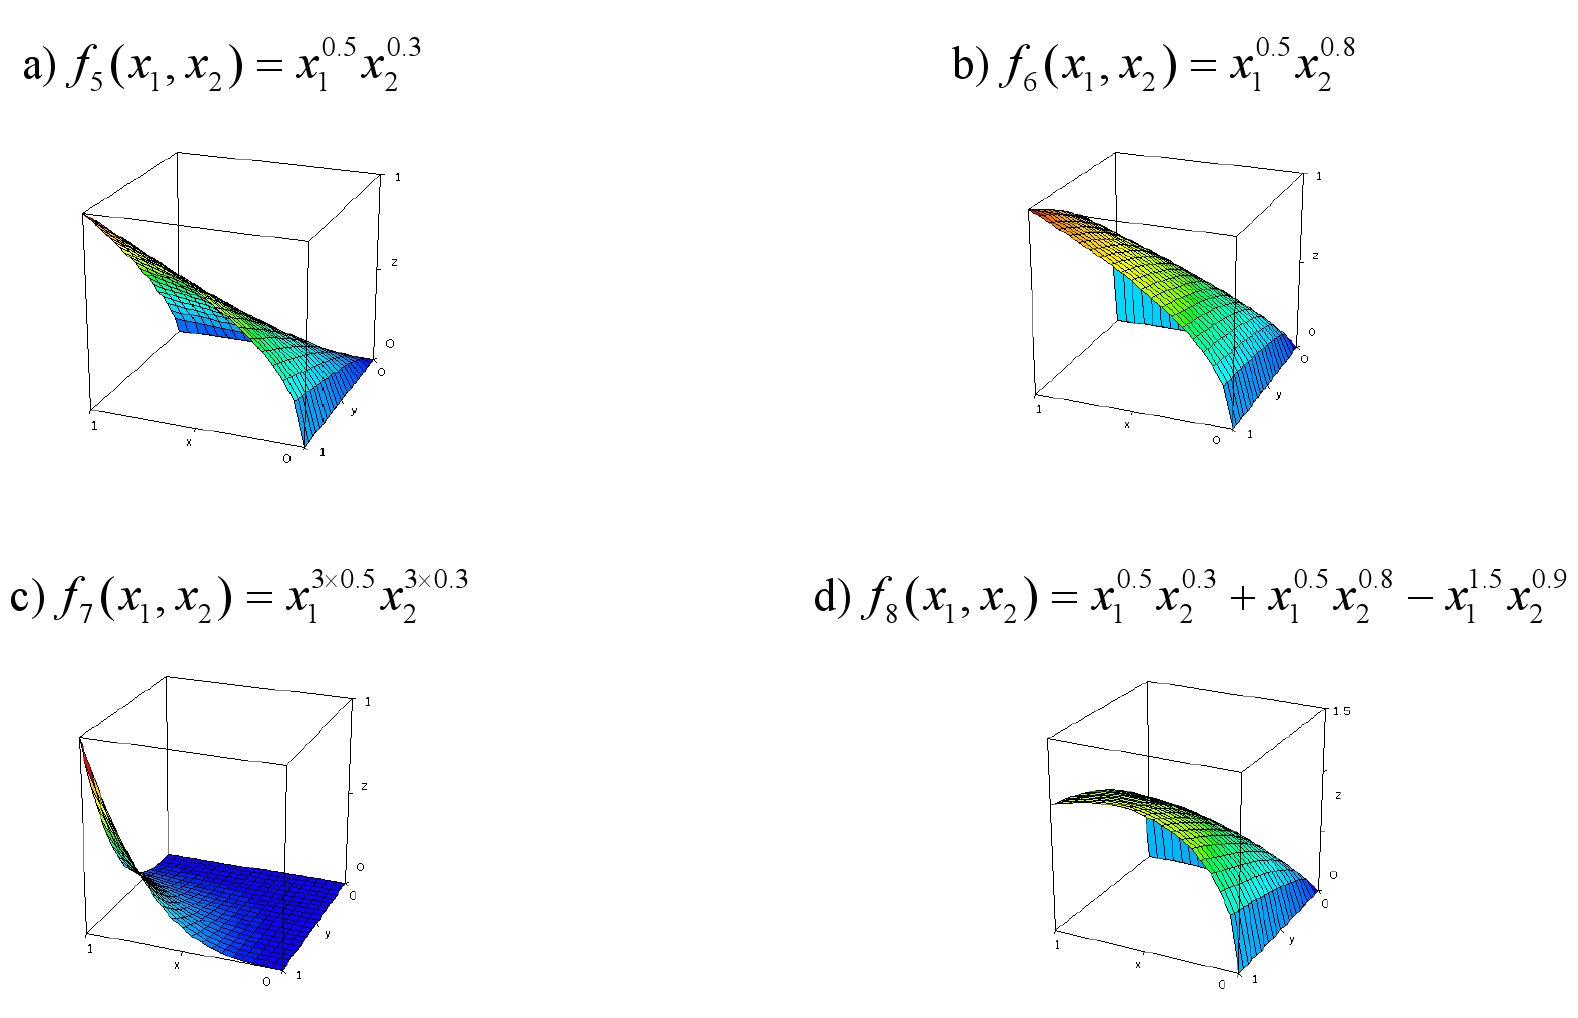
\includegraphics[keepaspectratio,width=12.5cm]{figuras/ejemploProducto.jpg}
\caption{Ejemplos de funciones de base producto, PUs.}
\label{ejemploProducto}
\end{figure}

\subsection{Redes con unidades de base radial}
\noindent     Los nodos ocultos de las ANNs con RBFs presentan funciones de activación de
tipo ventana.  Cada uno  de  los  nodos  RBF  realiza  una
aproximación local  independiente del  espacio  de búsqueda,  normalmente  mediante  una
campana  de Gauss.  La  capa  de  salida  de  tipo lineal  auna  el efecto  independiente
de  cada nodo,  sumando  cada  valor  obtenido.  La  idea  es  que cada  nodo  esté
situado en un entorno del espacio de búsqueda formado por las variables de entrada y
además con un radio determinado. El proceso de aprendizaje de la red de RBFs consistirá en
ir moviendo dichos nodos a lo largo del espacio de búsqueda, modificando los centros y los
radios de los mismos, para ajustarlos de la mejor forma a los datos de entrenamiento.

La  función  de  activación  será  equivalente  a  la  función  de  distancia
euclídea  (tomando  como centro de la RBF el vector $\mathbf{w}_{j}$), y la
función de
transferencia será una función de tipo Gaussiano. Por tanto, la función de
salida o transferencia sería la siguiente:
\begin{displaymath}
B_{j}\left(\mathbf{x},\mathbf{w}_{j}\right)=
e^{-\frac{1}{2}\left( \frac{d\left( \mathbf{x},\mathbf{w}_{j}\right) }{r_{j}}\right) }
\end{displaymath}
siendo
\begin{displaymath}
	d\left( \mathbf{x},\mathbf{w}_{j}\right) =\lVert
	\mathbf{x}-\mathbf{w}_{j}\rVert=\sqrt{\sum_{i=1}^n \left( x_{i}-w_{ij}\right)^2 }
\end{displaymath}
siendo $w_{ij}$ el peso asociado a la neurona $j-esima$ de la capa oculta y la neurona
$i-esima$ de la capa de entrada.

Algunas de las características de las redes RBF son:
\begin{enumerate}
		\item Se ha demostrado que las ANNs con unidades RBF son aproximadores
		universales \cite{Park1991}.
		\item En comparación con las redes MLP, las redes RBF presentan la
		ventaja de que	cada nodo en la capa oculta es un elemento local en el modelo, lo
		que hace que para	un	determinado patrón sólo algunas unidades ocultas se activen.
		Esta característica	facilita	el entrenamiento, disminuyendo el número de óptimos
		locales y regiones	planas de la superficie de error, al desaparecer gran parte
		de las	interacciones entre los pesos.
		\item Por último, el proceso de entrenamiento de una red MLP consta
		de una sola etapa, mientras que las redes RBF suelen entrenarse en dos etapas,
		siendo las	funciones	de base aproximadas en primer lugar mediante técnicas de
		aprendizaje no supervisado, determinando los centros y el número de funciones de
		base mediante, por ejemplo, un algoritmo $k$-medias,  y los	pesos	entre las capas
		oculta y de salida en segundo lugar,	mediante métodos supervisados.
\end{enumerate}

En la figura \ref{ejemploRadial} se muestra un ejemplo gráfico de la superficie generada
por el efecto aditivo de tres neuronas \textit{RBF}.
\begin{figure}[htb]
\centering
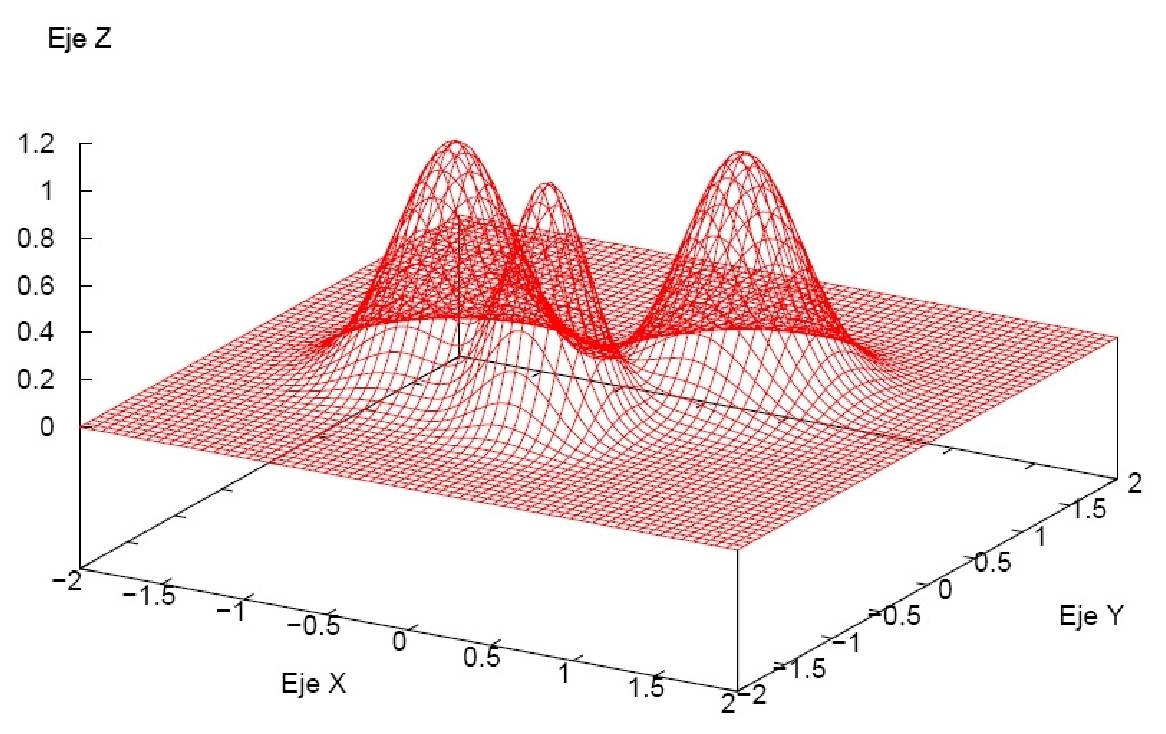
\includegraphics[keepaspectratio,width=12.5cm]{figuras/ejemploRadial.jpg}
\caption{Ejemplos de funciones de unidad de base radial, RBF.}
\label{ejemploRadial}
\end{figure}

\subsection{Redes híbridas}\label{redesHibridas}
\noindent Hasta este momento las ANNs que hemos definido poseían un solo tipo de
unidad de base como nodos de la red en la capa oculta, ya fuesen SUs, PUs o RBFs.

La combinación de diferentes funciones de base en capa oculta puede tener varias
ventajas si se consideran tareas de clasificación que tienen áreas generalmente
separadas, pero en las cuales es difícil situar su borde de decisión, debido a que las
mejores funciones discriminantes para cada clase del problema pueden ser muy diferentes.
Una mixtura de unidades de base puede proporcionar bordes de decisión flexibles,
cubriéndose las desventajas que puedan tener el uso de modelos con un solo tipo de unidad
de base o modelos puros. Donoho \cite{Donoho1989} demostró que cualquier función continua
se puede descomponer en dos tipos de funciones mutuamente excluyentes, una función
asociada con funciones de tipo proyección, SUs o PUs, y la otra asociada con funciones de
tipo ventana, RBFs. A pesar de
ello, en la práctica, es difícil separar las diferentes
localizaciones de una función y estimar la función residual mediante una aproximación
funcional basada en proyecciones, sin quedar atrapado en óptimos locales en la
minimización del error \cite{Friedman1991}.

Varios autores han propuesto la hibridación de redes con diferentes funciones de base, ya
sea con una sola capa oculta híbrida o interconectando varias capas puras. De acuerdo a
Duch y Jankowski \cite{Duch2001}, la hibridación de diferentes funciones de transferencia
dentro de una ANN se puede hacer de dos maneras. Una de ellas sería utilizar un método
constructivo que seleccione la mejor función de base a partir de un conjunto de funciones
RBF candidatas \cite{Duch2001a}; y un segundo método
sería partir de redes con diferentes unidades de base, y usar técnicas de poda o de
regularización para reducir el número de funciones \cite{Duch2001, Jankowski2001}.

Pao \cite{Pao1992} presentó una combinación de varias funciones (polinómicas, periódicas,
sigmoidales y gaussianas) en lo que llamó redes de enlace funcional (\textit{Functional
Link Networks}). La idea consistía en el uso de enlaces funcionales, añadiendo
transformaciones no lineales de las variables de entrada al conjunto original de variables,
y suprimiendo la capa oculta, haciendo una la primera aproximación no lineal fija, y una
segunda aproximación adaptativa.

Una aproximación más compleja considera varias capas o modelos, cada una conteniendo una
estructura de funciones de base, dando como resultado un sistema modular. Por ejemplo,
Iulian
\cite{Iulian2002} propuso una metodología incluyendo tres módulos distintos, implementando
una ANN hacia delante (llamada red neuronal RBF de tipo gaussiana), un proceso de
análisis de componentes principales, y una red SU. Otra
propuesta, de Lehtokangas and Saarinen \cite{Lehtokangas1998}, considera dos capas ocultas
en el modelo, la primera compuesta por funciones gaussianas y la segunda por SUs.

Las ANNs que utilizan diferentes funciones de base deberían contener
menos nodos, permitiendo que la función desempeñada por la red sea
más transparente. Por ejemplo, un hiperplano se puede utilizar para dividir
un espacio de entrada en dos clases y una función adicional de Gauss
que tenga en cuenta cualquier anomalía local. El análisis de la aproximación realizada
por una red MLP entrenada con los mismos datos no es tan simple. En este contexto cabe
señalar el trabajo de Cohen e Intrator \cite{Cohen2002a}, que se basa en las propiedades
de dualidad y complementariedad de las funciones de tipo proyección y de tipo ventana.

Recientemente, Wedge \cite{Wedge2006} presentó una ANN
híbrida compuesta por unidades de base RBFs y SUs. Se utiliza un algoritmo de
entrenamiento en tres pasos, en el cual se intentan identificar los aspectos de
una relación funcional que son expresados separadamente de aquellos que varían solo dentro
de las regiones particulares del espacio de entrada.

En \cite{Kordik2010}, se propone un algoritmo evolutivo llamado \textit{GAME} para la
optimización de la topología de una ANN, combinando diferentes tipos de neuronas,
entrenadas dentro de la red mediante varios algoritmos de optimización y principios de
meta-aprendizaje, para construir finalmente una ANN supervisada hacia delante con varias
capas y con varias funciones de base por capa.

Otros autores como Hervás \cite{Hervas2007,Hervas2007a}, hacen uso de
un AE que utiliza la función de entropía cruzada para evaluar a los
individuos de la población. Dicha población se compone de ANNs híbridas con una sola
capa oculta compuesta por unidades de tipo PUs y SUs. El algoritmo se encarga
de evolucionar simultáneamente la arquitectura y los pesos de cada red, utilizando un
operador de mutación adaptado a cada tipo de unidad de base. Los resultados
reflejan que la hibridación puede ser una alternativa viable con respecto a los
modelos puros en determinados problemas, y deja abiertas algunas cuestiones sobre
la posibilidad de crear procedimientos que permitan elegir
entre diferentes familias de funciones durante la evolución de las ANNs.
En \cite{Gutierrez2007,Gutierrez2009} se realiza una mejora del método anterior,
mediante la inclusión de un procedimiento de doble elitismo en el algoritmo evolutivo, y se da
 la posibilidad de utilizar tres tipos diferentes de redes, en función del tipo de
unidades de base usadas, redes Producto-Sigmoide (PSU), Producto-RBF (PRBF),
Sigmoide-RBF (SRBF). Algunas conclusiones de este trabajo
muestran que la elección adecuada del tipo de base a utilizar depende fuertemente del
conjunto de datos a clasificar, pero que, en general, los modelos compuestos por SUs y RBFs
consiguen un rendimiento mayor que los compuestos por SUs y PUs, especialmente en aquellos
conjuntos de datos con dos clases, donde solamente existe una función discriminante.
También se comprueba empíricamente que los modelos formados por SUs y PUs no consiguen una
precisión mayor que los restantes tipos de hibridación, aunque si consiguen tener un menor
número de conexiones, permitiendo que sean más interpretables.

A continuación, presentamos el modelo funcional o función de salida de una red
neuronal formada por diferentes tipos de unidades de base en su capa oculta (ver figura
\ref{ejemploHibrida}):
\begin{equation}\label{modelofhibrido}
f_{q}\left(\mathbf{x},\mathbf{\Theta}_{q} \right)= \alpha_{0}^q +\sum_{j=1}^{m1}
B_{j}^q \sigma_{j} \left( \mathbf{x},\mathbf{u}_{j}\right)+\sum_{k=1}^{m2}
\beta_{k}^q B_{k} \left( \mathbf{x},\mathbf{w}_{k}\right),
\end{equation}
donde $q$ es el número de unidades, nodos o neuronas de salida de la red,
$\displaystyle
\mathbf{\Theta}_{q}=\left(\alpha_{0}^q,\alpha_{1}^q,...,\alpha_{m1}^q,\beta_{0}^q,\beta_
{1}^q,...,\beta_{m2}^q,\mathbf{u}_{1},...,\mathbf{u}_{m1},
\mathbf{w}_{1},...,\mathbf{w}_{m2} \right)$ son los vectores de pesos de la neurona de
salida $q$, $\displaystyle \mathbf{u}_{j}=\left( u_{0}^j,u_{1}^j,...,u_{K}^j\right) $ y
$\displaystyle \mathbf{w}_{k}=\left( w_{0}^k,w_{1}^k,...,w_{K}^k\right) $ es el vector de
pesos de las conexiones entre la capa de entrada y la neurona oculta $j$ y $k$, $m1$ es el
número de neuronas ocultas del tipo 1 y $m2$ el el número de neuronas ocultas del tipo 2,
$K$ el número de neuronas o características en la capa de entrada,
$\mathbf{x}$ el valor de las entradas de la ANN, $\displaystyle B_{j}
\left( \mathbf{x},\mathbf{u}_{j}\right)$ es la función de base de la neurona $j$ de tipo 1
, $\displaystyle B_{k}
\left( \mathbf{x},\mathbf{w}_{k}\right)$ es la función de base de la neurona $k$ de tipo 2
y $\displaystyle \alpha_{0}^q$ y $\displaystyle u_{0}^j$ son los sesgos del modelo
asociado a la neurona $q$ en la capa de salida y a la neurona $j$ en la capa oculta
respectivamente.

\begin{figure}[htb]
\centering
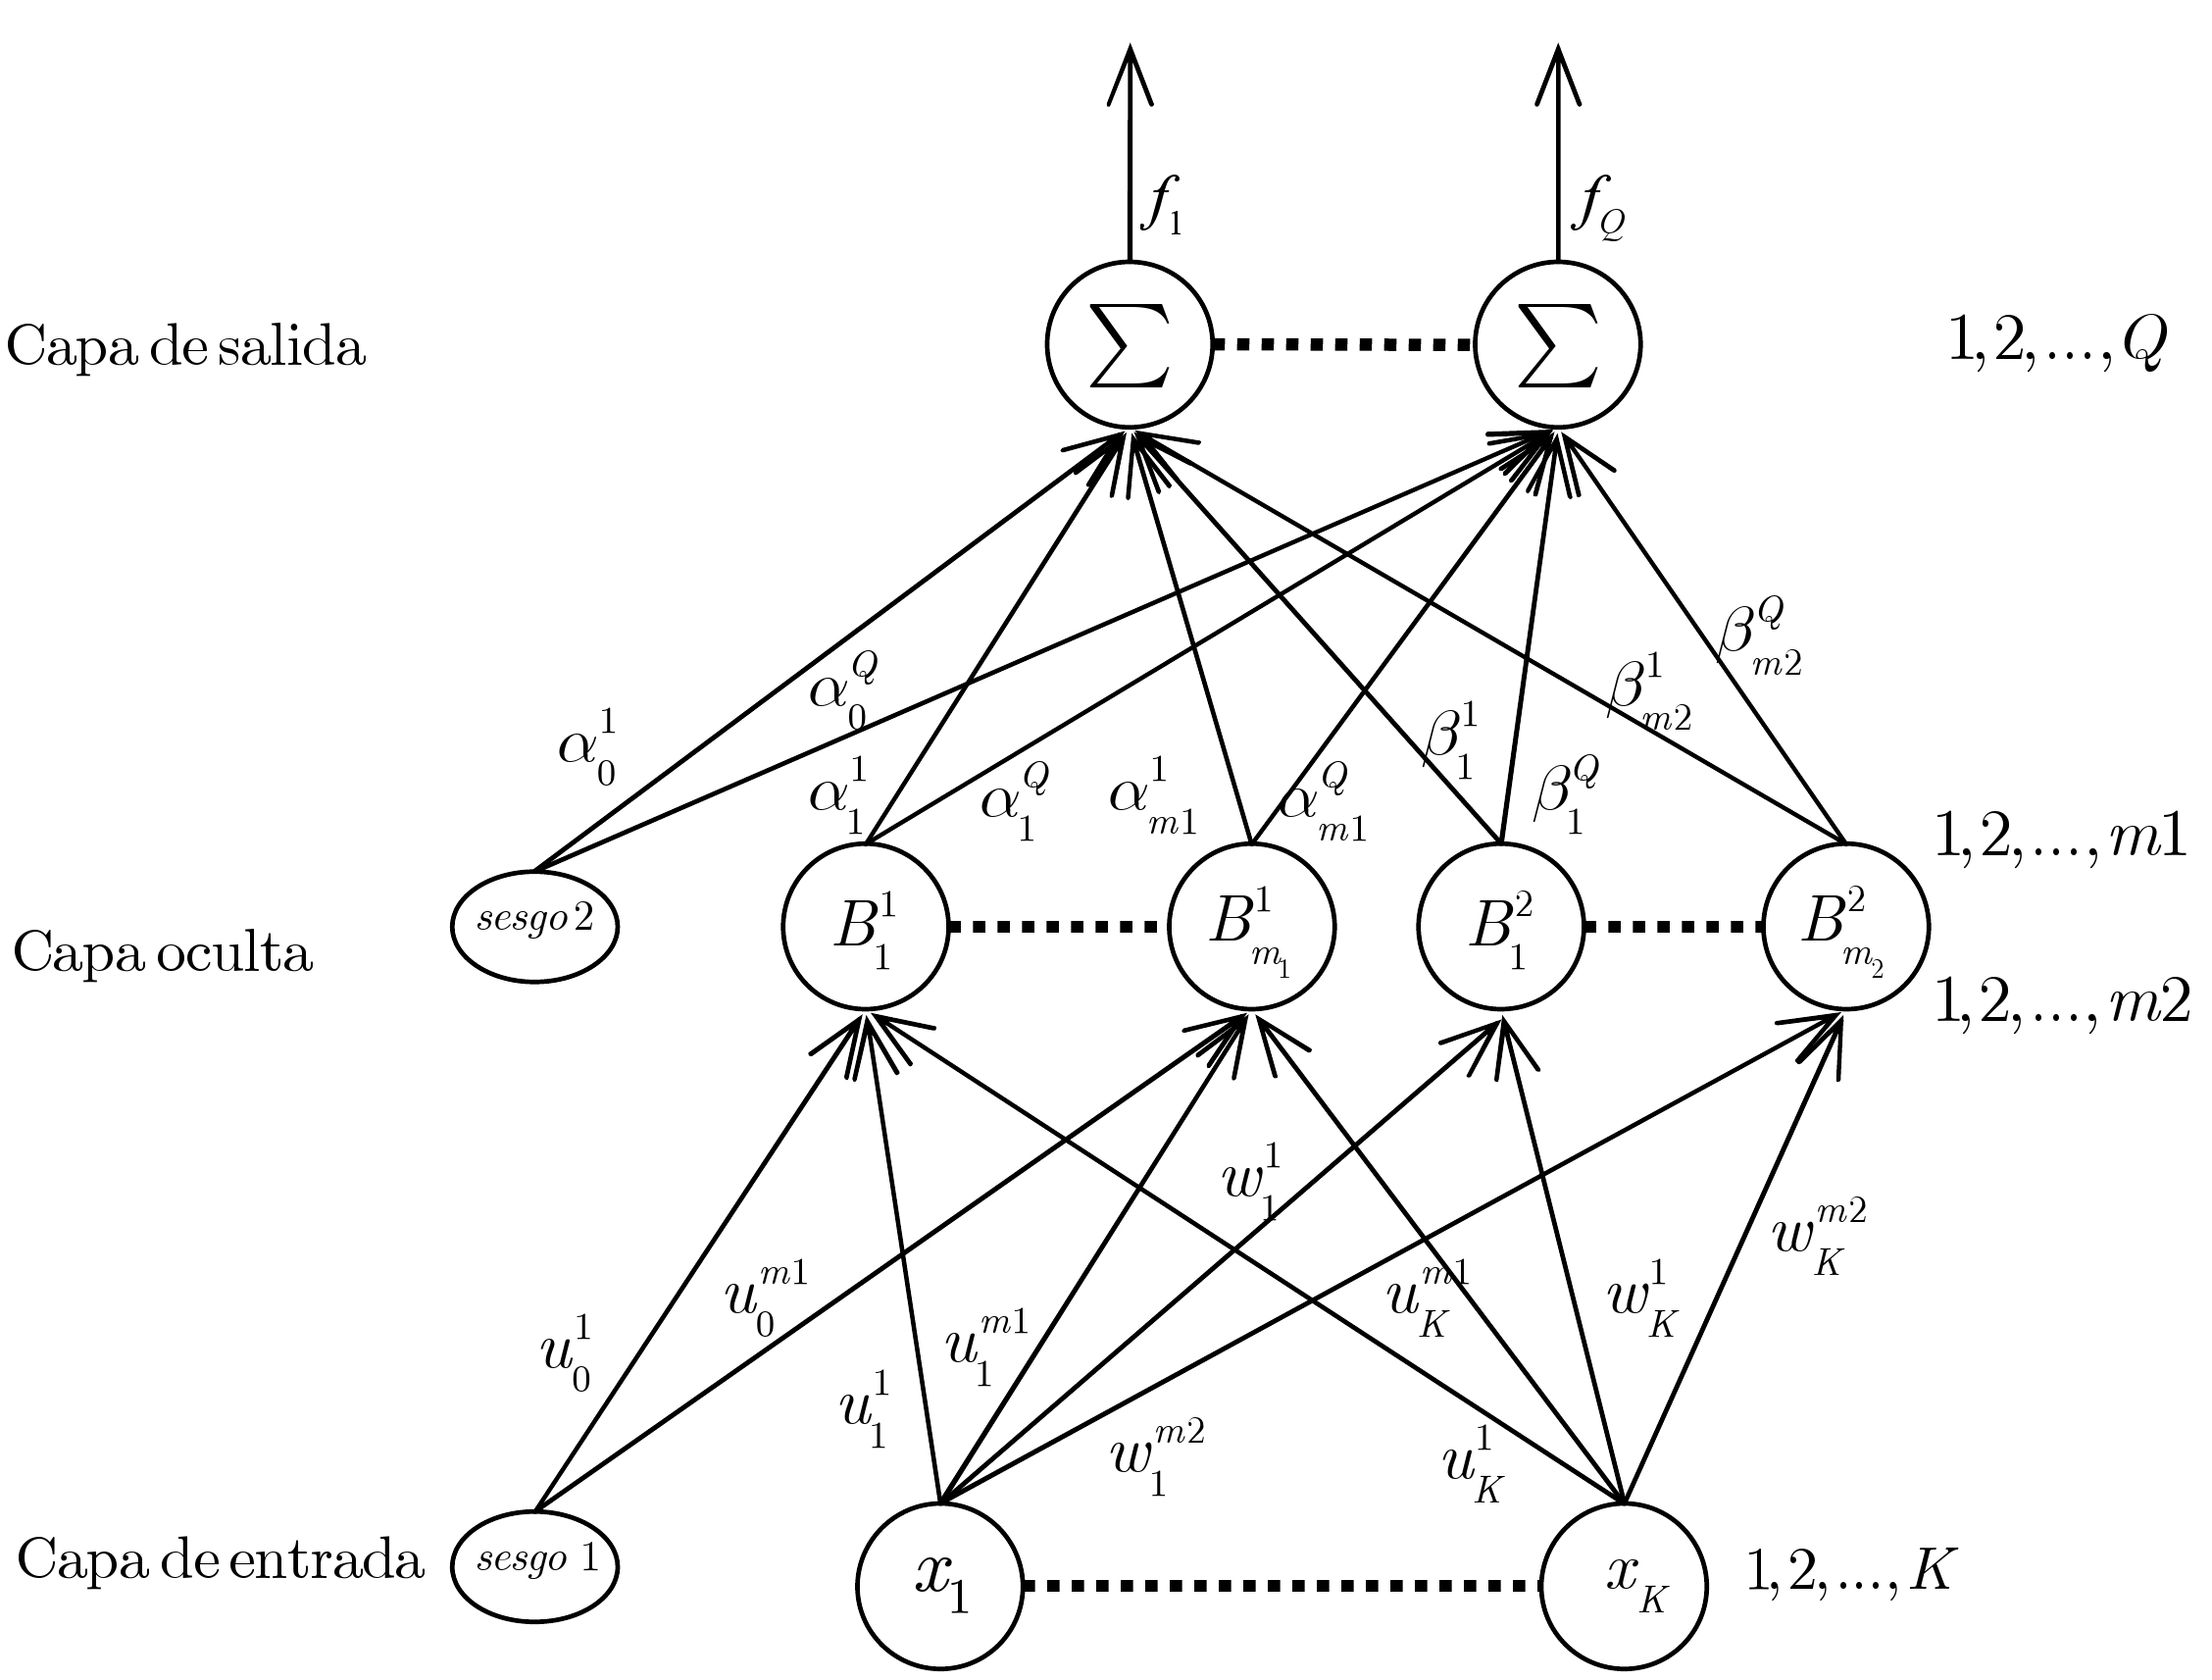
\includegraphics[keepaspectratio,width=12.5cm]{figuras/redHibridaHaciaDelante.jpg}
\caption{Red híbrida hacia delante con dos tipos diferentes de funciones de base en capa
oculta.}
\label{ejemploHibrida}
\end{figure}

% COGER EL PAPER DE NEUROCOMPUTING PARA METER LA TEORIA y el MODELO FUNCIONAL DE SALIDA
% TAMBIEN COGER EL DEL MAEB ``2007_maebA.PDf
\newpage
\section{Métodos de entrenamiento}\label{metodosEntrena}
A continuación se expone brevemente una visión global de los
métodos clásicos de optimización utilizados para el entrenamiento de ANNs, y de los
métodos que incorporan algún tipo de heurística o técnica para mejorar el aprendizaje
\cite{Kordik2010}.

\subsection{Métodos clásicos}\label{mClasicos}
\noindent La mayoría de los métodos clásicos utilizados para el entrenamiento de
ANNs tienen el problema de que pueden llegar a estancarse en una
solución que no sea lo suficientemente idónea para el problema que se
esté intentando resolver. Los métodos más comunes son:
\begin{description}
\item[Métodos constructivos:] Los métodos constructivos comienzan con una red mínima y
van añadiendo nodos y conexiones hasta que ésta es capaz de resolver el problema planteado
con una determinada precisión. Lo que se hace es adaptar el tamaño de la red al problema
en cuestión, teniendo la ventaja de que no se necesita hacer una estimación “a priori” del
tamaño de la misma, pero se necesita un experto con suficiente experiencia y un proceso de
prueba y error \cite{Burgess1994,Setiono1995}. Este tipo de métodos son susceptibles
de caer en mínimos locales \cite{Angeline1994}, además de que solo pueden llevar a cabo la
búsqueda en subconjuntos reducidos del espacio de las posibles
topologías.
\item[Métodos destructivos o de poda:] Los métodos destructivos o de poda
\cite{Reed1993,Reed1999} parten de una red suficientemente grande (inicialmente puede
sobre-entrenar y ser demasiado compleja), y sucesivamente se van eliminando nodos y
conexiones hasta llegar a una topología en la que la eliminación de un nodo no mejore los
resultados. La ventaja de estos métodos es que las redes se que obtienen son pequeñas y por
lo tanto más fáciles de implementar y entrenar. De nuevo, es primordial la experiencia del
diseñador, y se necesita un proceso de prueba y error.
\item[Métodos basados en gradiente:] El algoritmo de retropropagación
(\textit{BackPropagation}, BP) \cite{Chauvin1995} y sus múltiples variantes
\cite{Hush1993,Moller1993,Chauvin1995}
(ver siguiente sección) es uno de los más carismáticos y utilizados dentro de los métodos
basados en gradiente. Este tipo de metodologías tienen como principal inconveniente el
poder caer en óptimos locales y quedar estancado el proceso de aprendizaje, por lo que es
necesario establecer
de antemano una serie de parámetros, como por ejemplo la tasa de aprendizaje, la
inicialización de los pesos (influye en la rapidez del aprendizaje y en que se alcance o
no el mínimo global de la función de error), número de capas ocultas y número de neuronas
en cada capa, entre otros.
\end{description}

Los algoritmos clásicos suelen presentar una serie de problemas \cite{Angeline1994,
Yao1999}:
\begin{enumerate}
\item Imposibilidad de calcular el gradiente cuando la función de activación no es
derivable.
\item Incapacidad de encontrar un mínimo global si la función de error es multimodal
y/o no diferenciable.
\item Ausencia de convergencia de los algoritmos clásicos de entrenamiento cuando el
número de dígitos utilizados para representar la
función de activación o los pesos de la red (precisión) no es suficientemente grande.
\item Tendencia, por parte de los algoritmos de entrenamiento, a obtener excesivas
soluciones no óptimas en cada ejecución.
\item En general, los métodos constructivos y destructivos limitan las arquitecturas
disponibles. En algunos de éstos métodos, una vez se ha explorado una arquitectura y se ha decidido
que es insuficiente, se adopta una nueva arquitectura,
de manera que las antiguas arquitecturas se convierte en inalcanzables. Además, los
algoritmos constructivos y destructivos basan su estudio en subconjuntos topológicos,
en lugar de basarse en la clase completa de las arquitecturas de red. En consecuencia,
estos	algoritmos tienden a optimizar una clase de arquitectura en lugar de ajustar una
arquitectura apropiada para un problema determinado.
\item Las deficiencias de los métodos constructivos y destructivos se derivan de
métodos 	inadecuados para la asignación de los componentes estructurales
de una red. Se asumen que las restricciones topológicas limitan la complejidad de las
interacciones	estructurales y paramétricas, e incrementan la probabilidad de
encontrar una red suficiente buena para resolver el problema, pero lo ideal sería que
esas restricciones proviniesen de la tarea o problema en si, y no que estuvieran
implícitas en el algoritmo.
\item Otros métodos usan una sola modificación estructural predefinida, como añadir una
unidad completamente conectada en capa oculta, para generar topologías sucesivas.
Tales métodos como la escalada en colina estructurada (\textit{Structural Hill
Climbing}), son susceptibles de quedar atrapados en óptimos locales estructurales, y
hacen recaer la carga de la tarea de inducción principalmente en la
identificación de los valores adecuados de los parámetros, en vez de distribuir
la carga uniformemente.
\end{enumerate}

\subsection{Métodos heurísticos}\label{redesheuristicas}
\noindent La utilización de métodos de naturaleza heurística
\cite{Walczak1999,Abraham2000,Glover2003} para el entrenamiento de ANNs surge
en la década de  los  90  como  solución a los  problemas  de  entrenamiento presentados
por los algoritmos clásicos. A continuación se citan algunos de los métodos heurísticos
utilizados con más frecuencia para el aprendizaje de ANNs:
\begin{itemize}
	\item Variantes heurísticas de la retropropagación del error
	\cite{Riedmiller1994}, BP con velocidad adaptativa y/o optimización de
	los parámetros de aprendizaje \cite{Zainuddin2005}, la regla \textit{delta-delta} o la
	regla	\textit{delta-bar-delta} \cite{Jacobs1988}, algoritmo \textit{Quikprop}
	\cite{Veitch1991}, algoritmo \textit{iRprop+} \cite{Igel2000}.
	\item Algoritmos de gradiente conjugado como el \textit{FRCG} de Fletcher-Reeves
	\cite{Fletcher1964}, el \textit{PRCG} de Polak-Ribiére  \cite{Polak1969}
	o	el	de Powell-Beale \cite{Powell1977}.
	\item Algoritmos de tipo \textit{Quasi-Newton} como el \textit{DFP} de
	Davidon-Fletcher-Powell	\cite{Davidon1991} y el
	\textit{BFGS} de Broyden-Fletcher-Golfarb-Shannon	\cite{Broyden1970}.
	\item Algoritmos que modifican el método \textit{Quasi-Newton} como el \textit{LM} de
\\
	Levenberg-Marquard \cite{Marquardt1963}.
	\item Métodos heurísticos no basados en gradiente como el enfriamiento simulado
	(\textit{Simulated Annealing} , SA), la búsqueda  tabú (\textit{Tabu Search}, TS), la
	búsqueda dispersa (\textit{Scatter Search}, SS),
	los enjambres de partículas (\textit{Particle Swarm}, PS) y los algoritmos evolutivos
	(\textit{Evolutionary Algorithms}, EAs), siendo éstos últimos los que más impacto han
	tenido en el diseño de ANNs.
	Este	tipo de heurísticas se han utilizado muy frecuentemente para el	aprendizaje en
	ANNs \cite{Kordik2010,Alba2006}.
\end{itemize}

\paginavaciacompleta
		%\paginavaciacompleta
		%\chapter{Redes neuronales artificiales evolutivas mono-objetivo}\label{evoMonoObjetivo}
% \begin{quotation}
% \begin{small}
% 		\textit{El pesimista es un optimista con experiencia.}\\
% 		\textit{El pesimista es una persona previsora y bien informada.}
% \end{small}
% \begin{flushright}
% François Truffaut.\\
% Anónimo.
% \end{flushright}
% \end{quotation}
\section{Motivación}
\noindent En este capítulo hablamos fundamentalmente del diseño de ANNs híbridas mediante
AEs, usando un
algoritmo al que hemos llamado CBFEP (\textit{Combined Basis Function Evolutionary
Programing})
\cite{Gutierrez2009,Gutierrez2007}. Este algoritmo fue diseñado como paso previo al diseño
de ANNs mediante algoritmos evolutivos multi-objetivo, (\textit{Multi-Objective
Evolutionary Algorithms}, MOEAS) \cite{Deb2004,Coello2007}, ya que en un futuro pensamos
incorporar ANNs híbridas junto con MOEAs para el diseño de modelos de red para
multi-clasificación de
patrones.

A continuación se muestra una breve introducción sobre el entrenamiento de ANNs con AEs y
sobre
las metodologías existentes, para posteriormente dar paso al algoritmo CBFEP.

\section{Entrenamiento de redes neuronales evolutivas}\label{enganio}
\noindent La Computación Evolutiva (\textit{Evolutionary Computation},
EC) \cite{Holland1992}, es una rama de la ciencia que interpreta la naturaleza como una
inmensa máquina de resolver problemas, y trata de encontrar el origen de dicha
potencialidad para reutilizarla en sus propias aproximaciones.
% El concepto de EA describe un conjunto de sistemas para resolver problemas mediante el
% ordenador, que usan un modelo computacional similar a los procesos evolutivos existentes
% en la naturaleza. Es decir, un modelo basado en el principio darwiniano de reproducción
% y
% supervivencia de los individuos que mejor se adaptan al entorno en que viven.

La utilización de métodos de naturaleza heurística para el entrenamiento de ANNs
surge en la década de los 90 (ver sección \ref{redesheuristicas} del capítulo
\ref{redesneuronales}). Las motivos principales que sugieren el uso de este tipo de
técnicas vienen determinados, en gran medida, por las limitaciones presentadas y
comentadas anteriormente por los algoritmos clásicos de aprendizaje (ver sección
\ref{mClasicos} del capítulo \ref{redesneuronales}). Dentro de los métodos
heurísticos, los EAs son los más utilizados para el diseño de modelos de red, ya
que presentan una metodología muy útil a la hora de optimizar la topología y los pesos de
una ANN, y existen muchas aplicaciones al respecto, tanto para clasificación de patrones
\cite{Bishop2006,Fu2004,Scheme2007,Paliwal2009} como para regresión
\cite{Valero2007,Hervas2007c,Hervas2007b,Hervas2009,Gutierrez2008,Gutierrez2009a,
Gutierrez2009b,Gutierrez2009d}. Los EAs \cite{Back1996,Back1997,Eiben2003} son eficientes
para encontrar un conjunto de pesos para las conexiones cercanas al óptimo, sin utilizar información
sobre el gradiente, y
la función de aptitud de los individuos no tiene porque ser diferenciable. Los EAs pueden
tratar espacios complejos, no diferenciables y multimodales. La evolución de las
arquitecturas de ANNs permite adaptar sus topologías a diferentes tareas sin la
intervención humana, y por lo tanto, proporciona una aproximación al diseño de las mismas
de manera automática, ya que tanto los pesos de conexión y como la arquitectura se pueden
evolucionar.

El entrenamiento de ANNs mediante EAs es un buen ejemplo para llevar a
cabo el dilema explotación/exploración en un algoritmo de búsqueda \cite{Lozano2008}.
Este método de aprendizaje puede resultar lento si se compara con otros métodos de
entrenamiento clásicos, sin embargo, los EAs son muchos menos sensibles a las condiciones
iniciales del entrenamiento, buscan una solución
global y óptima y no requieren el cálculo del gradiente. Si tenemos en cuenta
la dificultad que implica el establecimiento de una arquitectura adecuada junto con el
aprendizaje de los correspondientes pesos de la ANN, la utilización de EAs para el
diseño de la estructura y la optimización de los coeficientes de una ANN está
ampliamente justificada.

De la utilización de los EAs para la optimización de ANNs surgen las
denominadas Redes Neuronales Artificiales Evolutivas (\textit{Evolutionary
Artificial Neural Networks}, EANNs) \cite{Yao1999}. El lector puede consultar varios
trabajos y estados del arte sobre este aspecto
en \cite{Zhang2000,CantuPaz2005,Ludemir2006,Ou2007}.

Existen varias formas \cite{Yao1999} de abordar el entrenamiento de una
ANN con un EA, aunque son tres las más utilizadas:
\begin{description}
\item[Evolución de los pesos:] En este caso se fija la arquitectura de la red, número de
capas ocultas, número de nodos en capa oculta y número de conexiones, y se
desarrolla una búsqueda global en el espacio de los pesos (valores de las conexiones).
Esta técnica conlleva tener una gran experiencia por
parte de los diseñadores, y realizar procedimientos de prueba y error, partiendo de
diferentes topologías para un problema en cuestión. Además, es muy importante la elección
de los operadores genéticos de recombinación que se utilicen y la codificación de los
pesos que se haga (en la actualidad la codificación se hace mediante números reales).
\item[Evolución de la arquitectura:] Seleccionar la arquitectura
de una ANN es una difícil tarea, y las EANNs pueden encontrar
automáticamente una buena arquitectura que no produzca sobre-entrenamiento o falta de
aprendizaje en el conjunto de generalización. En este caso, se
suele partir de una inicialización aleatoria de los pesos y, tras la ejecución de un
EA, se suelen realizar varias iteraciones de un algoritmo BP clásico.
El diseño de una arquitectura óptima de una ANN se puede formular como un
problema de búsqueda en el espacio de arquitecturas, donde cada punto representa una
arquitectura diferente. Dados algunos criterios de rendimiento, como por ejemplo el error
más bajo de entrenamiento, la menor complejidad de red, etc, el nivel de rendimiento de
todas las arquitecturas forma una superficie discreta. El diseño de la
arquitectura óptima es equivalente a encontrar el punto más alto de esta superficie.
\item[Evolución de los pesos y la arquitectura simultáneamente:] Con esta \newline estrategia se
evolucionan simultáneamente los pesos y la arquitectura de la red. Cada individuo de la
población especifica tanto la arquitectura como los pesos de conexión. El operador
genético que se suele utilizar es la mutación, tanto paramétrica (modificación de los
pesos de la ANN) como estructural (modificación de la topología). El cruce en
ocasiones puede que no proporcione buenos resultados, ya que recombinar una parte de una
ANN con otra parte de otra, posiblemente hará que ambas redes pierdan
funcionalidad \cite{Angeline1994}. Por otra parte, existe el problema de la permutación o
del engaño \cite{Yao1999}, que consiste en que dos redes que ordenan
sus nodos ocultos en forma diferente tienen distinta representación, pero pueden ser
funcionalmente equivalentes, con lo que la probabilidad de producir una mejor descendencia
por recombinación a partir de ellas es baja. Por ejemplo, las ANNs mostradas
por las figuras \ref{enganio1a} y \ref{enganio2a} son equivalentes, pero tienen distintas
representaciones del genotipo, como se ve en las figuras \ref{enganio1b} y
\ref{enganio2b}, usando el esquema de codificación directo. En general, cualquier
permutación de los nodos ocultos producirá ANNs funcionalmente equivalentes,
pero con distintas representaciones del genotipo. A pesar de ello hay autores que no
consideran este problema demasiado importante y sugieren que cambiando los tamaños de
población y la selección de individuos se reduce considerablemente.

\begin{figure*}[htb]
\centering
\subfloat[]{\label{enganio1a}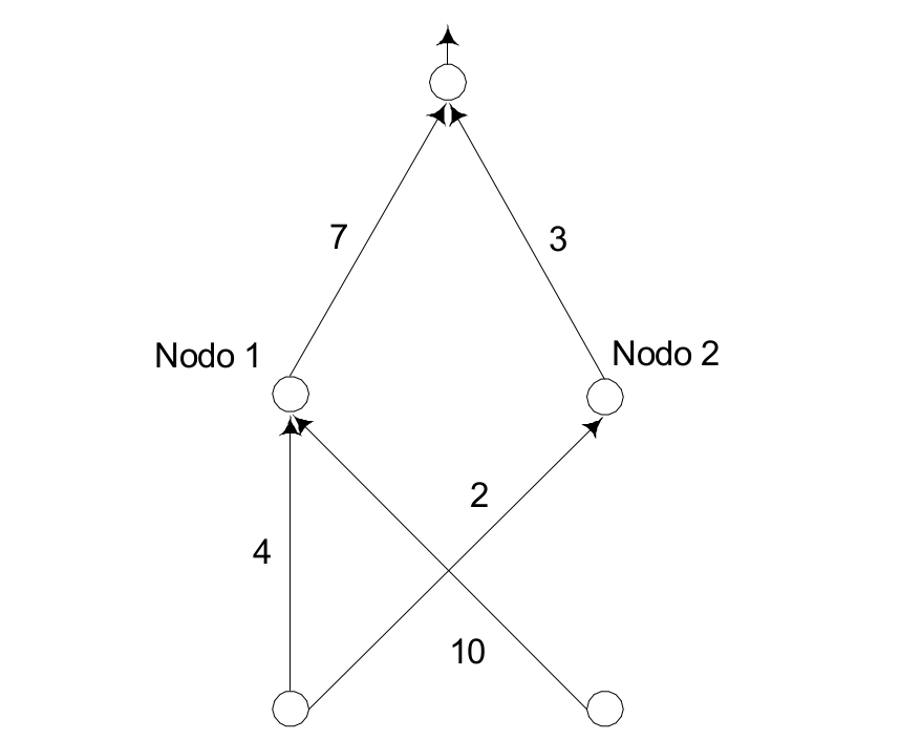
\includegraphics[width=.35
\textwidth]{figuras/enganio_1a.jpg}}
\subfloat[]{\label{enganio1b}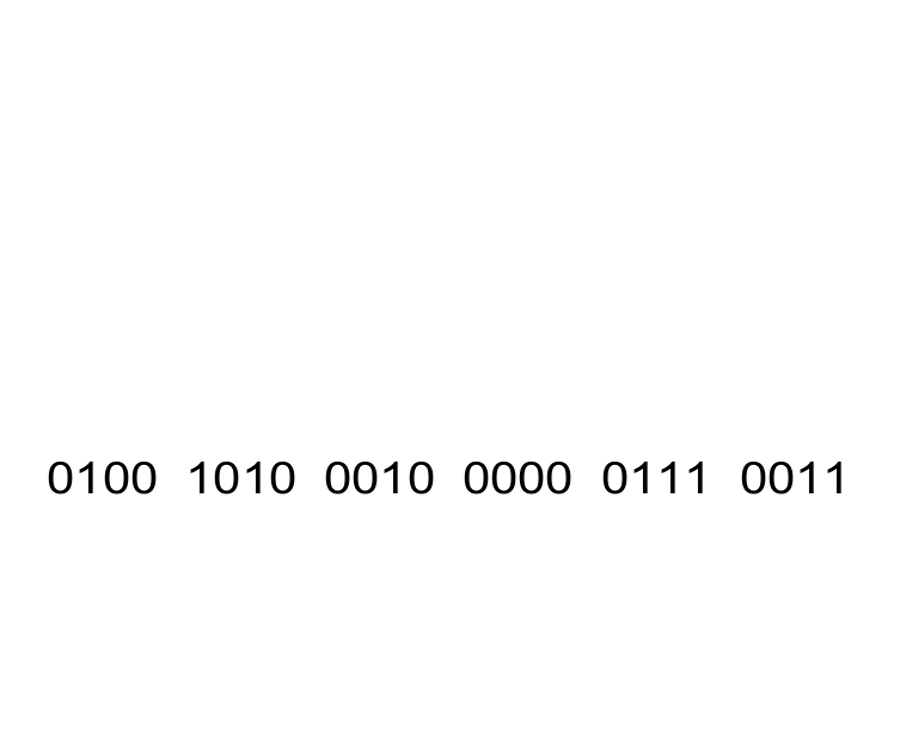
\includegraphics[width=.35
\textwidth]{figuras/enganio_1b.jpg}} \\
\subfloat[]{\label{enganio2a}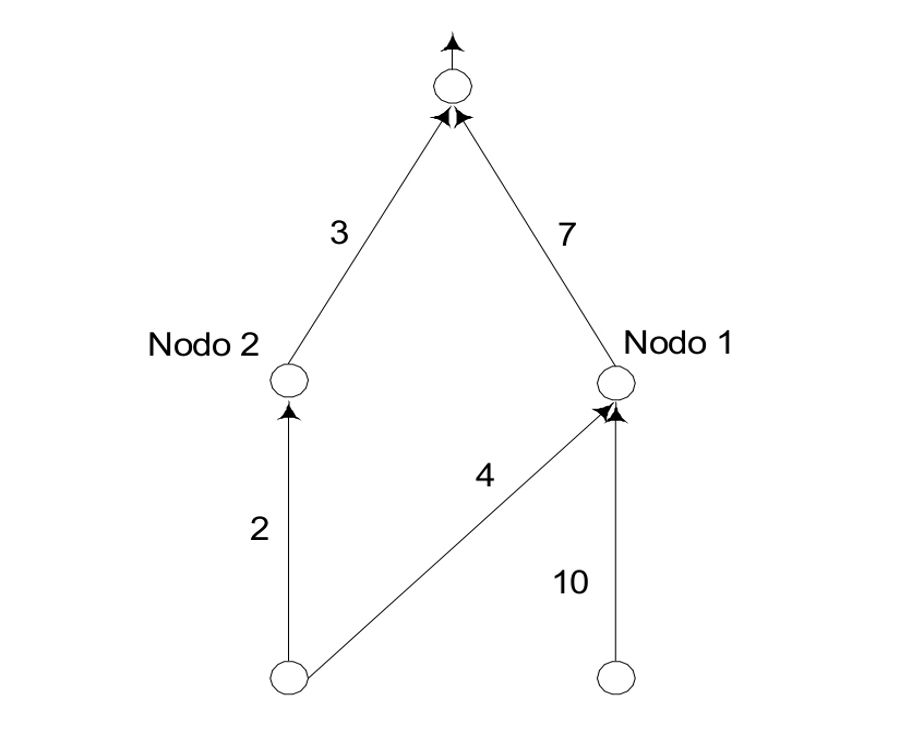
\includegraphics[width=.35
\textwidth]{figuras/enganio_2a.jpg}}
\subfloat[]{\label{enganio2b}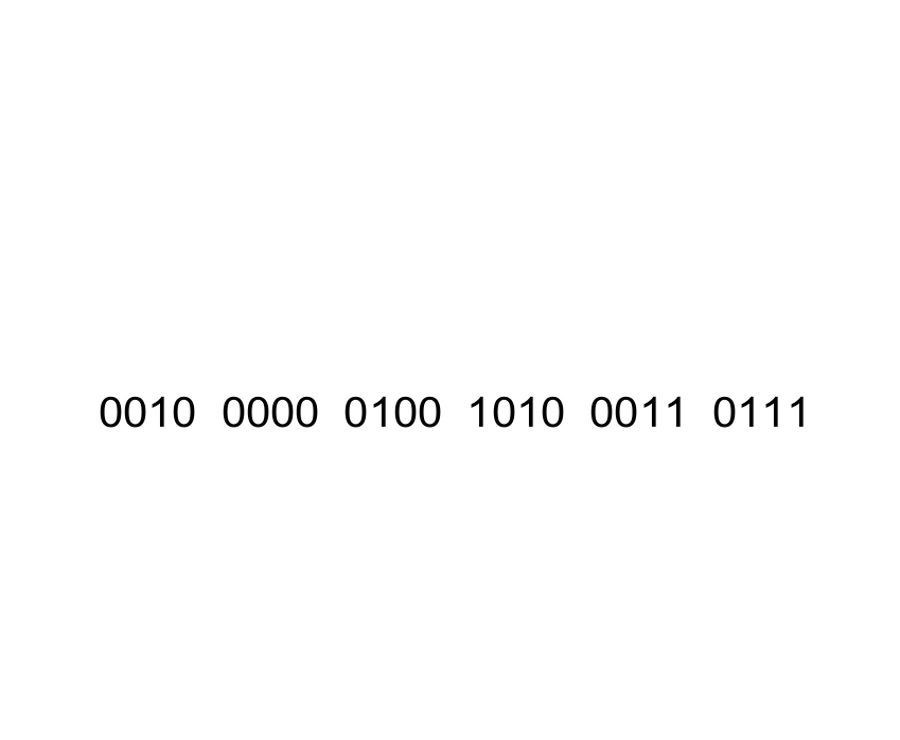
\includegraphics[width=.35
\textwidth]{figuras/enganio_2b.jpg}}
\caption{Problema de la permutación. En a) y c) se muestran dos redes
equivalentes y en b) y d) sus representaciones genotípicas.}
\label{enganio}
\end{figure*}
% \item[Evolución de las reglas de aprendizaje:] Otro tipo de evolución en
% \textit{ANNs} (aunque menos usada) es la evolución de las reglas de aprendizaje junto
%con
% los pesos de la red \cite{Baxter1992}.
% Este tipo de evolución tiene que realizarse en entornos dinámicos pero estableciendo una
% serie de restricciones, como por ejemplo la forma básica de la regla de aprendizaje,
%para
% así reducir la complejidad de la representación, y una serie de asunciones: la
% actualización de los pesos depende solo de información local, y la regla de
% aprendizaje es la misma para todas las conexiones en una ANN.
\end{description}

\section{Codificación de redes neuronales evolutivas}\label{codificacion}
\noindent Es importante comentar que la codificación que se haga de la ANN
influye en el proceso del diseño de la misma. Hay dos tipos de codificación (ver con más
detalle en \cite{Yao1999}) :
\begin{description}
\item[Directa:] La arquitectura de la red se codifica directamente sobre un cromosoma,
describiéndola en todos sus aspectos, incluyendo los pesos de la misma. Este diseño  se
puede  realizar  conjuntamente  con  la  estimación  o  aprendizaje  de  los pesos,  o
hacerlo independientemente, usando un cromosoma para los pesos y otro para la
arquitectura. Este tipo de codificación permite definir con facilidad operadores de cruce
y de mutación, sin embargo, el problema de la codificación directa es que en el caso de
que las estructuras sean grandes crece su representación, lo que produce un algoritmo poco
eficiente. No obstante, existen posibilidades de reducir el tamaño de las matrices de
representación, si tenemos en cuenta algunas  de  las restricciones propias  de la  red
neuronal, como puede  ser que  no existan  conexiones entre los nodos de entrada.
\item[Indirecta:] Una codificación indirecta describe solamente la manera de
``ensamblar'' una ANN. El objetivo es minimizar la longitud del cromosoma que
representa a la estructura de la red, representando  algunas  características importantes
que la identifiquen. Un tipo de representación indirecta puede ser la representación
paramétrica, donde una red se puede representar como un conjunto de parámetros: número de
capas ocultas, número de nodos en cada capa y número de conexiones entre capas. Otro tipo
de representación indirecta puede ser mediante gramáticas, compuestas por reglas de
producción para construir arquitecturas. La codificación indirecta puede producir una
representación genotípica más compacta de la arquitectura de una red, pero quizás no sea
tan buena en la búsqueda de una red compacta con una buena capacidad de generalización.
\end{description}

En este trabajo de tesis el tipo de codificación que se utiliza es directa, pero no se
trabaja directamente con los pesos y/o estructura de la red, sino con una representación
orientada a objetos. Digamos, por tanto, que se trabaja a caballo entre el genotipo y el
fenotipo (interpretación del genotipo), ya que a cada una de las características de la
red se accede por medio de una clase \cite{Poo2007}. Cada conexión se especifica por un
valor binario, indicando si existe o no, y por separado se indica con un valor real el
peso de la misma. Como se verá más adelante no se considerarán operadores de cruce en la
evolución de los individuos de la población, con lo que no se asume un orden fijo entre
los distintos nodos ocultos. A nivel de programación e ingeniería del software, de manera
breve, cada ANN
queda representada
por: clases para representar las diferentes capas de la red (entrada, oculta,
salida) y el tipo de capa oculta, según esté formada por unidades puras o una hibridación
de estas; clases para representar el tipo de unidad de base, nodo o neurona
utilizados en cada capa (sigmoides, producto, base radial), y si es una neurona de entrada
o una neurona enlazada; y clases para representar enlaces entre dos nodos o neuronas y
su valor o peso.

En la siguiente sección exponemos un EA para el entrenamiento de ANNs híbridas como paso
previo a corto plazo de la incorporación de este tipo de ANNs a MOEAs.

\section{El algoritmo CBFEP}
\noindent Una vez comentadas las características básicas de un EA y las diferentes
metodologías usadas en la literatura para el entrenamiento de ANNs mediante EAs, pasamos
a describir un algoritmo que hemos diseñado para la obtención de modelos de red híbridos (ver
sección \ref{redesHibridas} del capítulo \ref{redesneuronales}) para clasificación de
patrones, teniendo en cuenta solo una función objetivo o función de aptitud. Hemos llamado
a este algoritmo CBFEP (\textit{Combined Basis Function Evolutionary Programing})
\cite{Gutierrez2007,Gutierrez2009}.

CBFEP es un EA que estima los parámetros y la estructura de la red de manera simultanea, lo que se
conoce como método TWEANN (\textit{Topology and Weight Evolving Artificial Neural
Networks}). La población de individuos está sujeta a operaciones de
replicación y de mutación, no usando operador de cruce debido a las desventajas
potenciales que ha demostrado tener en la evolución de ANNs
\cite{Angeline1994,Yao1999}. Al no utilizarse operador de cruce por el problema del
engaño, y teniendo en cuenta la forma de codificar las redes, CBFEP cae dentro del
paradigma de la Programación Evolutiva (\textit{Evolutionary Programming}, EP)
\cite{Fogel1966}.

En la figura \ref{marcoNNEP} se muestra el marco general de CBFEP, y en la figura
\ref{etapasNNEP} podemos ver una representación gráfica, claramente diferenciada, de las
etapas del mismo. Podemos consultar una estructura más básica de CBFEP en
\cite{Alfonso2006}.

En las siguientes subsecciones se irá detallando el procedimiento
utilizado en CBFEP, obteniendo como resultado final redes híbridas PSU (unidades de base
producto y sigmoide), redes PRBF (unidades de base producto y
de base radial) o redes SRBF (unidades de base sigmoide y de base radial), es
decir, CBFEP en este caso está encaminado a la obtención de modelos de red híbridos en
capa oculta.

\begin{figure}[htb]
\centering
\fbox{
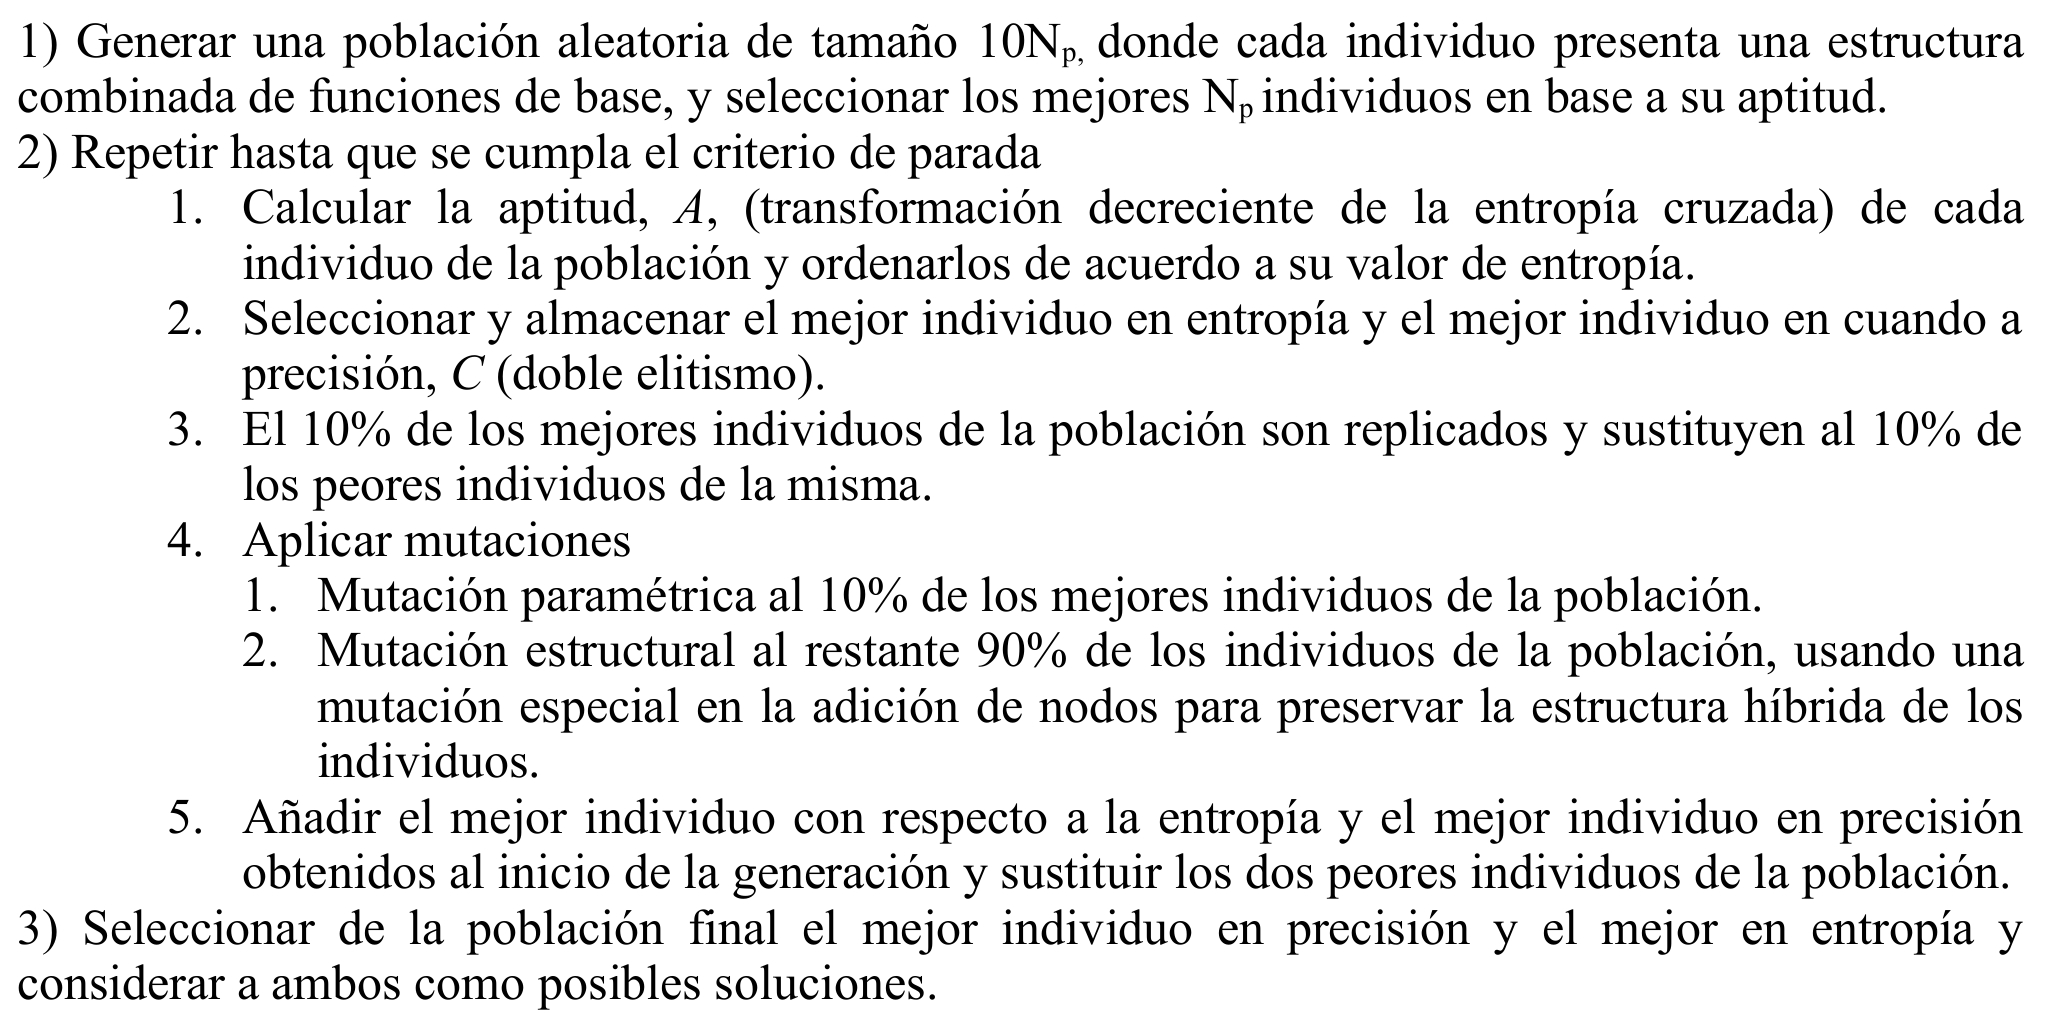
\includegraphics[keepaspectratio,width=12.5cm]{figuras/marcoNNEP.jpg}
}
\caption{Marco general del algoritmo CBFEP.}
\label{marcoNNEP}
\end{figure}
\begin{figure}[htb]
\centering
	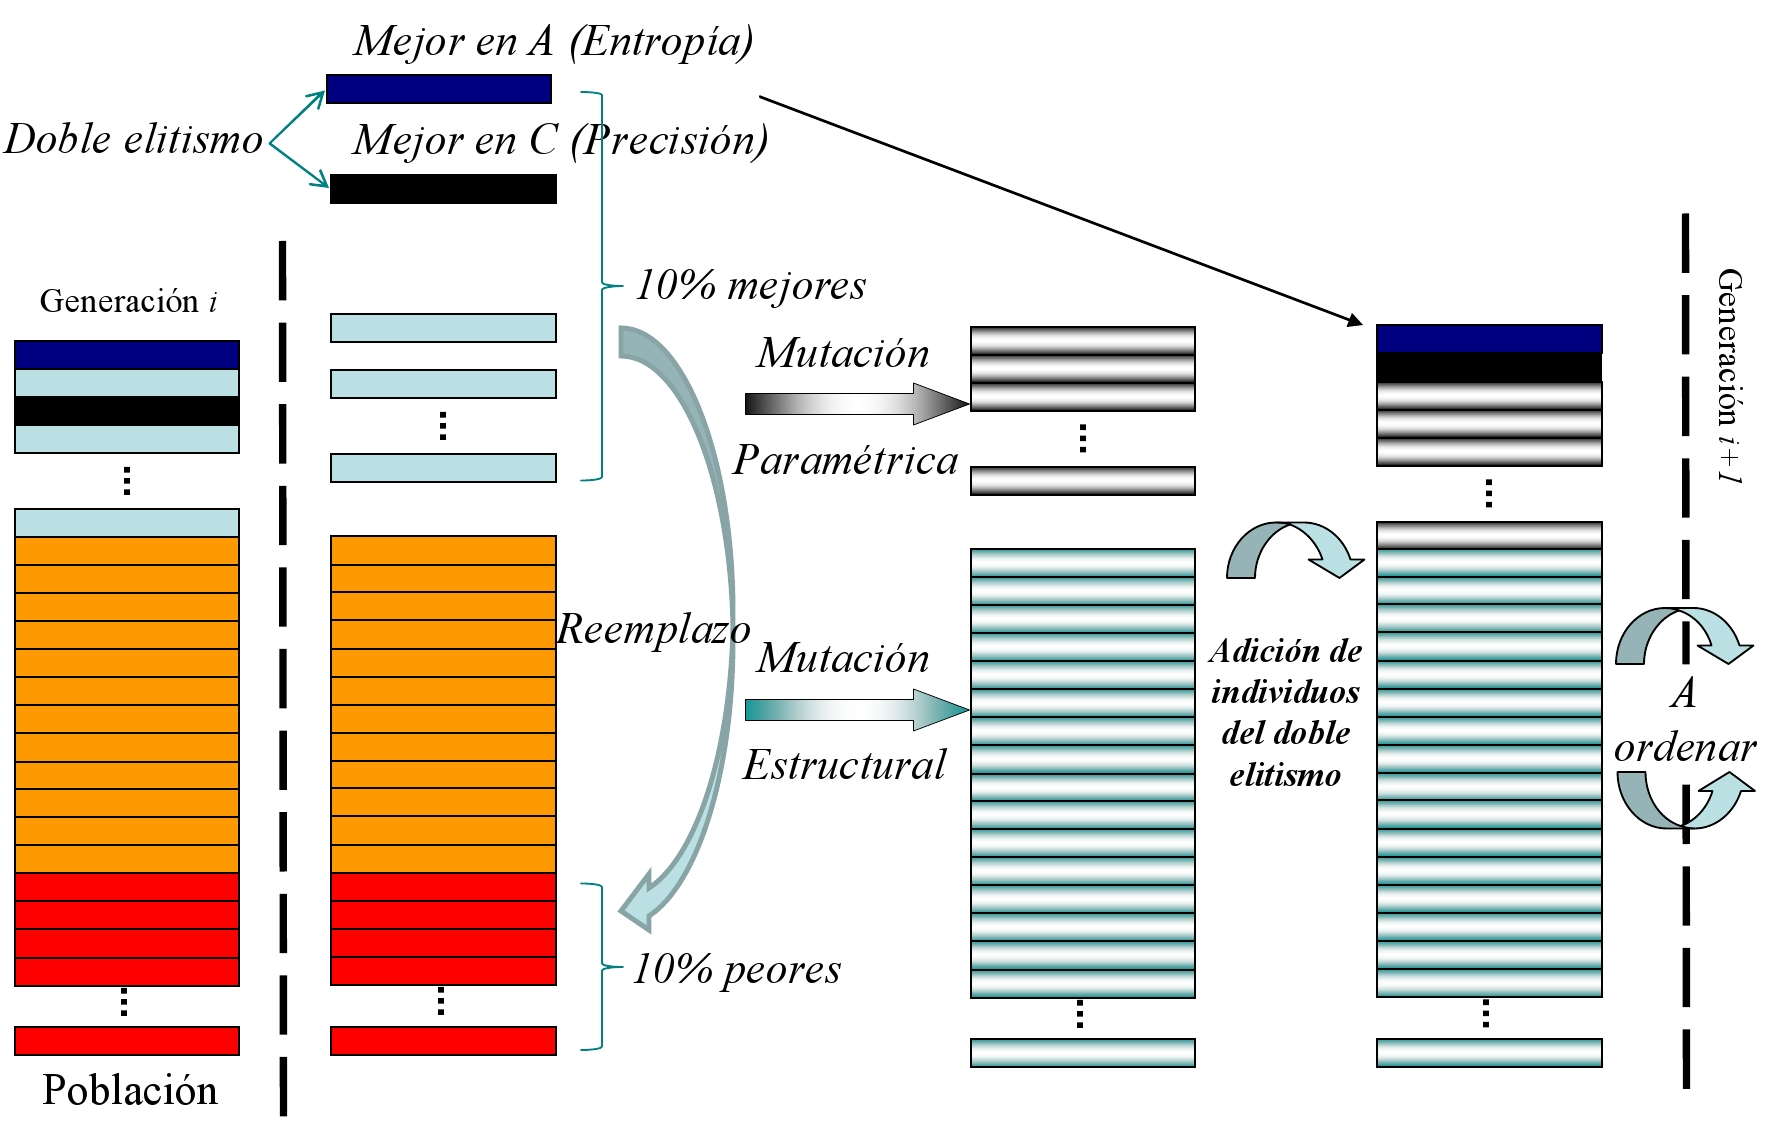
\includegraphics[keepaspectratio,width=12.5cm]{figuras/etapasNNEP.jpg}
\caption{Esquema del procedimiento de doble elitismo.}
\label{etapasNNEP}
\end{figure}
\newpage
\subsection{Función objetivo}
\noindent La función de aptitud que usamos con el algoritmo CBFEP, es una transformación
estrictamente decreciente de la función de entropía cruzada, $E$, comentada en la sección
\ref{metricasmulticlase} del capítulo
\ref{medidasRendimiento}. Teniendo en cuenta el modelo funcional asociado a las redes
híbridas y a la función $E$, la aptitud viene dada por:
\begin{equation}\label{aptitudNNEP}
A\left( g,\mathbf{\Theta}\right) =\frac{1}{1+E\left( g,\mathbf{\Theta}\right)}
\end{equation}
Una ventaja de utilizar $E$ y no $(1-C)$ (como podría pensarse), es que $E$ es una función
continua, lo que hace que la convergencia sea más robusta. En varios estudios se ha
demostrado
que $E$, por norma general, tiene mayor robustez que $C$ en problemas de clasificación
\cite{Bishop1995,Bishop2006}.

\subsection{Operadores}\label{operadores}
\noindent Antes de comenzar a describir el algoritmo, describiremos los operadores
de mutación utilizados en CBFEP durante el proceso evolutivo. Estos se dividen en
mutaciones estructurales y una mutación paramétrica.

Las mutaciones estructurales constan de 5 tipos:
% \begin{itemize}
% 	\item \textbf{Añadir neurona, (\textit{Add Neuron}, AN):} Consiste en añadir
% neuronas a
% la red.
% 	\item \textbf{Eliminar neurona, (\textit{Delete Neuron}, DN):} Consiste en eliminar
% neuronas	de la red.
% 	\item \textbf{Añadir enlace, (\textit{Add Link}, AL):} Consiste en añadir nuevos
% enlaces
% a la	red.
% 	\item \textbf{Eliminar enlace, (\textit{Delete Link}, DL):} Consiste en
% eliminar enlaces
% de la	red.
% 	\item \textbf{Unir neuronas, (\textit{Fusion Neurons}, FN):} Consiste
% en la unión o
% fusión de dos nodos de la red.
% \end{itemize}
\begin{description}
\item [Añadir neurona, (\textit{Add Neuron}, AN):] Consiste en añadir neuronas a la red.
\item [Eliminar neurona, (\textit{Delete Neuron}, DN):] Consiste en eliminar neuronas	de
la red.
\item [Añadir enlace, (\textit{Add Link}, AL):] Consiste en añadir nuevos enlaces a la
red.
\item [Eliminar enlace, (\textit{Delete Link}, DL):] Consiste en eliminar enlaces de la
red.
\item [Unir neuronas, (\textit{Fusion Neurons}, FN):] Consiste en la unión o fusión de dos
nodos de la red.
\end{description}

Según el paso 4.2 de la figura \ref{marcoNNEP}, al 90\% de los individuos de la
población se le aplica una de las 5 mutaciones estructurales comentadas anteriormente.
Para ello disponemos de un valor de temperatura $T$ que posee cada individuo en base a su
aptitud, y que viene dado por $\displaystyle T(g)= 1-A(g)$. Aleatoriamente se escoge un
valor entre $\left[0,1\right]$, y si ese valor es menor que $T$, se aplica la primera de
las 5 mutaciones estructurales existentes en este orden: AN-DN-AL-DL-FN, de forma que si
la mutación ha sido exitosa el proceso de mutación del individuo termina. Si el valor
aleatorio es mayor que $T$, o por circunstancias especiales de topología, (no tener nodos
en capa oculta, que una neurona se quede sin conexiones o sin enlace a la capa de salida,
o que se sobrepase el número máximo de nodos establecidos ``a priori``, etc), la mutación a
aplicar no pudiera utilizarse (mutación no exitosa), se procedería del mismo modo a
aplicar el siguiente tipo de mutación de la lista, según el orden establecido. Si ninguna
mutación tiene éxito, se elige de manera forzosa y aleatoriamente cualquiera de las
mutaciones anteriores, siempre que no conlleve ninguna situación especial de la topología
de la red. A medida que nos aproximamos al final del proceso evolutivo,
la probabilidad de mutar a un individuo es menor, ya que su aptitud aumenta.

Las mutaciones AL y DL se aplican solamente en la capa oculta y en la
capa de salida, mientras que las mutaciones AN, DN y FN se
realizan en capa oculta. El número de neuronas a añadir o eliminar se elije
aleatoriamente entre los valores $\left[1,2\right] $, mientras que el número de enlaces a
añadir o eliminar depende del que haya en ese momento en cada red. Se añadirán o
eliminarán el 30\% del total
de enlaces que haya entre capa de entrada y capa oculta y el 5\% del total de los enlaces
existentes entre capa oculta y capa de salida.

\subsubsection{Mutación añadir neurona}
\noindent A la hora de añadir neuronas se hace tantas veces como número de neuronas
tengamos que añadir (depende del valor aleatorio obtenido). También se elegirá
aleatoriamente el tipo de unidad de base. Si una neurona no puede añadirse porque la capa
oculta ya posee el número máximo de neuronas posibles y establecidas al comienzo del
proceso evolutivo (ver subsección \ref{etapas}), la mutación se dará por no exitosa. En
caso de que el número de neuronas a añadir fueran dos y la primera si se hubiese añadido,
pero la segunda no, la mutación se dará por exitosa, es decir, con una sola adición de
neurona la mutación ya se considera correcta.

En cuanto a los pesos de los enlaces asociados a las neuronas añadidas, se establecen de
la siguiente manera:
\begin{itemize}
	\item Enlaces con la capa de entrada: El número de enlaces de entrada a añadir a la
	nueva neurona se escoge aleatoriamente en el intervalo definido por $\left[
	1,numeroEntradas\right]	$. El peso asignado a cada enlace es el mismo con el que se
	crean las redes al inicio del	proceso evolutivo, es decir, un valor aleatorio entre
	$\left[-1,1\right]$, pero es configurable. Para cada	enlace, la neurona de entrada
	se escoge aleatoriamente, y se añade, exista	o no. Si	existe se sobre-escribe su
valor.
	\item Enlaces con la capa de salida: El número de enlaces de salida a añadir a la
	nueva neurona se escoge aleatoriamente en el intervalo $\left[ 1,numeroSalidas\right]$.
	El peso asignado a cada enlace es el mismo con el se crean las redes al
	inicio, un valor aleatorio entre $\left[ -10,10\right] $, pero este parámetro es
	configurable. Para
	cada enlace, la neurona de salida se escoge aleatoriamente. En este caso, si se evita
	el sobre-escribir un enlace añadido anteriormente ya que su comprobación es menos
	costosa	computacionalmente porque que el número de neuronas de salida (número de
	clases) suele ser menor	que el de neuronas de entrada (número de atributos).
\end{itemize}

\subsubsection{Mutación eliminar neurona}
\noindent Se elige aleatoriamente la neurona que será eliminada, y se hace tantas veces
como numero de neuronas haya que eliminar, dependiendo del valor aleatorio obtenido. Si al
intentar borrar una neurona, la capa oculta ya posee el número mínimo de neuronas
establecidos al inicio del proceso evolutivo, se termina este tipo de mutación y se pasa a
al siguiente tipo. En caso de que el número de neuronas a eliminar fueran dos y la primera
sí se hubiese eliminado pero la segunda no, la mutación se dará por exitosa. Otro caso con
el que hay que tener especial cuidado es si la neurona escogida para eliminar, es la única
neurona con la cual está enlazada una neurona de capa de salida, entonces la neurona no se
elimina y se elige aleatoriamente otra sin tener en cuenta la anterior. Esto sirve para
evitar que en capa de salida nos aparezca una neurona que no tenga enlaces con ninguna
neurona de la capa oculta, o sólo tenga enlace con la neurona que representa el sesgo. Con
respecto a los enlaces asociados a la neurona/s eliminada/s, éstos también se eliminan.

\subsubsection{Mutación añadir enlace}
\noindent Se elige aleatoriamente la neurona de la capa que será mutada (neurona destino
del enlace) y la neurona de la capa anterior desde la cual añadiremos el enlace (neurona
origen del enlace). Esta mutación se hace
tantas veces como número de enlaces tengamos que añadir, según el total de enlaces que hay
entre capa oculta y capa de entrada y entre capa de salida y capa oculta. Si el enlace ya
existiese antes de aplicar la mutación, el enlace será sobre-escrito con el nuevo valor
del peso. Por tanto, esta mutación siempre tiene éxito.

\subsubsection{Mutación eliminar enlace}
\noindent El proceso de eliminación a la hora de escoger un enlace es el mismo que en la
mutación AL, pero teniendo en cuenta los siguientes casos especiales: Si el
enlace elegido es el único de la neurona destino, no se elimina. Si la neurona destino es
la neurona de salida y, aunque ésta tenga más enlaces, al quitarlo provocásemos que la
neurona oculta origen se quedase sin ningún enlace de salida, no se elimina. En estos
casos la mutación no tiene éxito.

\subsubsection{Mutación unir neuronas}
\noindent La mutación FN consiste en elegir aleatoriamente dos neuronas \textit{a} y
\textit{b}, y sustituirlas por otra nueva neurona \textit{c}. Si la capa oculta ya posee el
número mínimo de neuronas preestablecido, la mutación no tiene éxito (se pasaría al
siguiente tipo de mutación). Si la capa oculta es híbrida, las neuronas elegidas deben ser
del mismo tipo. Si no hay dos neuronas del mismo tipo, la mutación no tiene éxito(se
pasaría al siguiente tipo de mutación). Se conservarán los enlaces en la neurona \textit{c}
con los nodos comunes a las neuronas \textit{a} y \textit{b}, y también se conservan con
una probabilidad de $0.5$ los que no sean comunes. El resultado de la fusión queda así
(ver ejemplo en figura \ref{unirNodos}):
\begin{itemize}
\item Enlaces de entrada de la nueva neurona resultado de la unión: Por cada entrada, si
ambas neuronas originales poseían ese enlace de entrada, el enlace se conserva con un peso
igual a la media de ambos pesos. Si sólo una neurona poseía ese enlace de entrada, el
enlace se conserva con una probabilidad de $0.5$ y con el mismo peso. Si ninguna neurona
poseía ese enlace de entrada, la neurona resultado tampoco lo poseerá.
\item Enlaces de salida de la nueva neurona resultado de la unión: Por cada neurona de
salida, si ambas neuronas originales poseían ese enlace de salida, el enlace se conserva
con un peso igual a la suma de ambos pesos. Si sólo una neurona poseía ese enlace de
salida, el enlace se conserva con una probabilidad de $0.5$ y con el mismo peso. Si
ninguna neurona poseía ese enlace de salida, la neurona resultado tampoco lo poseerá.
\begin{displaymath}
u_{i}^c=\frac{u_{i}^a+u_{i}^b}{2}; \quad w_{i}^c=\frac{w_{i}^a+w_{i}^b}{2}; \quad
\alpha_{j}^c=\alpha_{j}^a+\alpha_{j}^b; \quad \beta_{j}^c=\beta_{j}^a+\beta_{j}^b
\end{displaymath}
para $i$ igual al número de neuronas en capa oculta y $j$ igual al número de neuronas en
capa de salida.
\end{itemize}

\begin{figure}[htb]
\centering
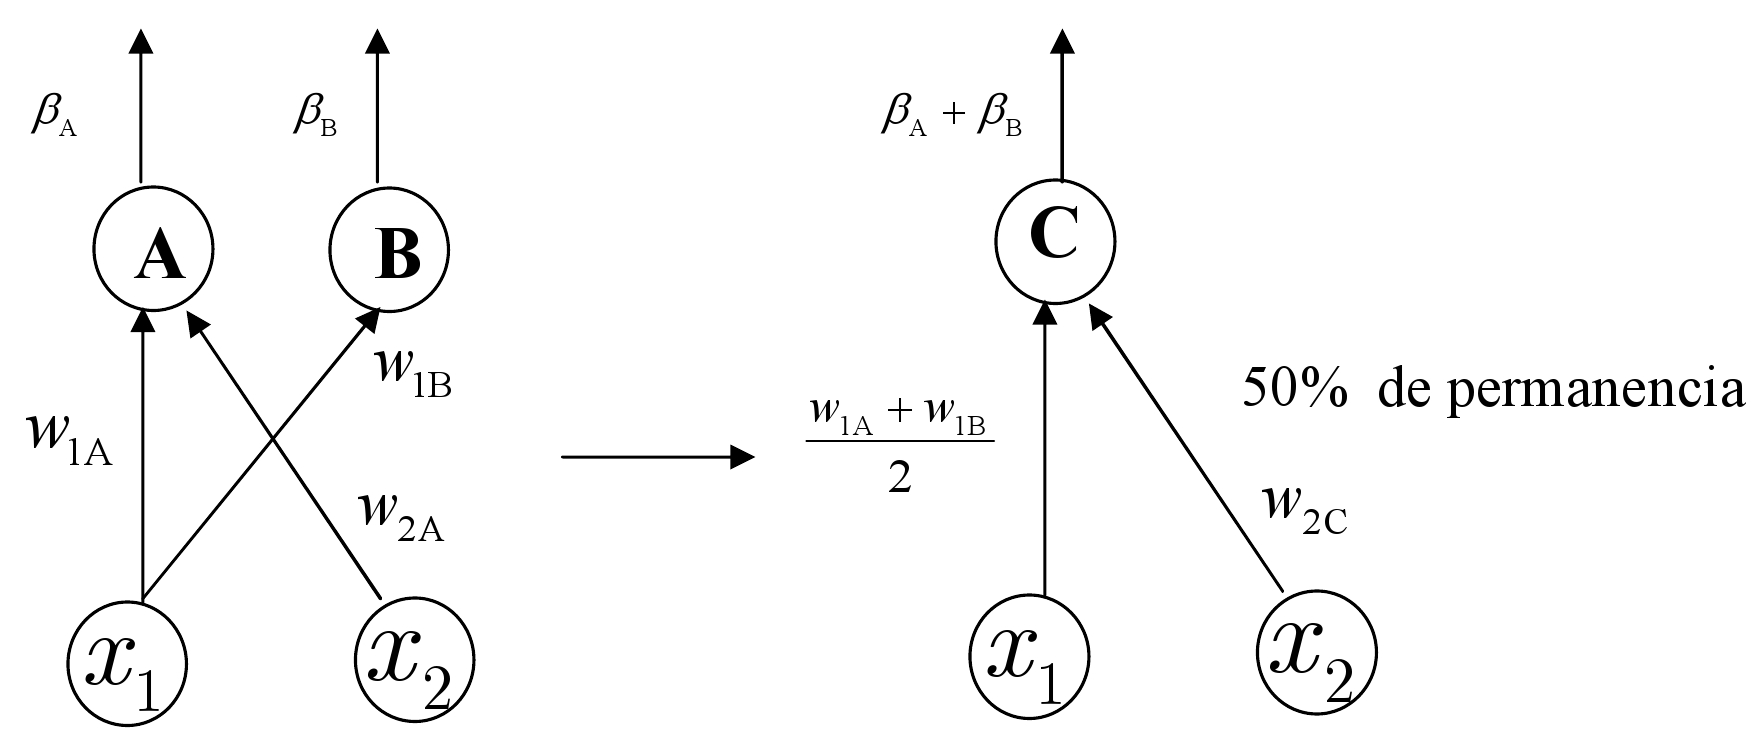
\includegraphics[keepaspectratio,width=10.5cm]{figuras/unirNodos.jpg}
\caption{Ejemplo de fusión de dos neuronas con la mutación FN.}
\label{unirNodos}
\end{figure}

En el caso de las neuronas RBF, la unión debe hacerse de otro modo, ya que el
significado de dichas neuronas es diferente, encargándose cada una de modelar una zona del
espacio cercana a su centro. El hecho de que las funciones combinadas puedan
interpretarse
como circunferencias de centro y radio perfectamente identificados obliga a que, al
combinar ambas neuronas, se tenga en cuenta este conocimiento topológico. Llamemos $
\mathbf{c}_j$ al centro definido por la neurona $j$, es decir,
$(w_{1j},w_{2j},...,w_{kj})$ y $r_j$
a su radio. En este caso, la mutación FN de dos neuronas RBF, $a$ y $b$,
consistirá en calcular el centro y radio de la neurona $c$ como:
\begin{center}
$\mathbf{c}_{c} =
$\begin{Large}$\frac{r_a}{r_a+r_b}$\end{Large}$\cdot \mathbf{c}_a
+$ \begin{Large}$\frac{r_b}{r_a+r_b}$\end{Large}$\cdot \mathbf{c}_b$
$\quad r_{c}=$\begin{Large}$\frac{r_a +
r_b}{2}$\end{Large}
\end{center}

\subsubsection{Mutación paramétrica}
\noindent La mutación paramétrica consiste en la alteración de todos los pesos de
la red (el sesgo también se muta paramétricamente), sumando un ruido gaussiano, donde la
varianza de la distribución de Gauss depende de la temperatura, $T$, definida
anteriormente. De esta forma, al principio del EA, cuando el proceso de
búsqueda se está iniciando, la aptitud de la red es cercana a cero y por tanto la
temperatura es alta, por lo que las mutaciones
son más grandes. A medida que nos acercamos al final del proceso evolutivo, disminuye la
temperatura, por lo que los cambios que se realizan en los pesos de las redes van siendo
más pequeños, afinando así la búsqueda.

Si consideramos el modelo funcional de la sección \ref{redesHibridas} del capítulo
\ref{redesneuronales}, los pesos de la capa intermedia quedarían
actualizados de la siguiente forma:
\begin{center}
$u_{ij}(t+1) = u_{ij}(t)+\xi_1(t)$\\
$w_{ij}(t+1) = w_{ij}(t)+\xi_1(t)$\\
$\theta_j(t+1) = \theta_{j}(t)+\xi_2(t)$\\
\end{center}
para $i$ igual al número de neuronas en capa de entrada y $j$ igual al número de neuronas
en capa de oculta, siendo $\xi_1(t)$ y $\xi_2(t)$ un valor aleatorio de la
distribución normal $N(0, \alpha_1(t)T(t))$, donde $\alpha_1(t)$ es un parámetro que junto
con la temperatura determina la varianza de la distribución, la cual varía durante la
evolución adaptando el proceso de aprendizaje, y $t$ el número de generación donde
se encuentra el EA.

Siguiendo esta misma filosofía, si la neurona a mutar es una unidad RBF, la
actualización del radio viene dada por $r_{j}(t+1) = r_j(t)+\xi_1(t)$.

En cuanto a los pesos de la capa de salida se actualizarán de forma análoga:
	\begin{center}
	$\alpha_{ij}(t+1) = \alpha_{ij}(t)+\xi_2(t)$\\
   $\beta_{ij}(t+1) = \beta_{ij}(t)+\xi_2(t)$\\
   \end{center}
para $i$ igual al número de neuronas en capa de salida y $j$ igual al número de
neuronas	en capa de oculta, y siendo $\xi_2(t)$ un valor aleatorio de la distribución
normal $N(0, \alpha_2(t)T(t))$, donde $\alpha_1(t)$ es un parámetro que junto con la
temperatura determina la varianza de la distribución, la cual varia durante la evolución
adaptando el proceso de aprendizaje. Se
cumple además que $\alpha_1(t) << \alpha_2(t)$,  es decir,   las mutaciones de los pesos
$w_{ij}$ y $\theta_j$,   correspondientes a los pesos con que se ponderan las variables
de la función que queremos modelar, han de ser menores que las   mutaciones realizadas en
los pesos $\beta_{ij}$,   correspondientes a los coeficientes de las unidades de base de
la función. Esto se debe a que el efecto de una mutación de un   peso que pondera a una
variable de entrada es mucho mayor que   el de un coeficiente, y por lo tanto los cambios
a realizar   deben ser menores.

Una vez realizado el cambio en el espacio de los pesos, la aptitud del individuo se
recalcula y se aplica un   algoritmo estándar de enfriamiento simulado. Si llamamos
$\triangle A$ a la variación de la aptitud antes y después del   cambio en los pesos,
resulta que:
   \begin{itemize}
   \item[-] Si $\triangle A\geq 0$, se acepta el cambio.
   \item[-] Si $\triangle A<0$, se acepta el cambio
   si \begin{Large}$e^{\frac{\triangle A}{T}}$\end{Large}
   $<\gamma$, donde $\gamma \in U(0,1)$
   \end{itemize}

Los parámetros $\alpha_1$ y $\alpha_2$  van cambiando durante el proceso de evolutivo
(al   contrario que la versión estática en \cite{Angeline1994}),   realizando en este
sentido un aprendizaje adaptativo. De esta   forma evitamos quedar atrapados en mínimos
locales y aceleramos		el proceso de evolución cuando las condiciones del proceso lo
permiten. Se debe escoger un mecanismo de evolución de los parámetros
$\alpha_1$ y $\alpha_2$ que converja más rápido hacia los      valores óptimos. El
mecanismo escogido en este caso es la regla  de razón de éxito 1/5 de Rechenberg, uno
de los métodos más simples. Según esta regla, la razón de mutaciones satisfactorias
debería ser siempre 1/5 \cite{Rechenberg1973}. De esta forma, si la razón es mayor que 1/5
la varianza debería incrementarse; en caso contrario,  debería disminuirse. Esto es:
      \begin{center}
      $
      \begin{array}{c} \\ \alpha_i(t+s) \\ i=1,2 \end{array} =
      \left\{
			\begin{array}{ccl}
         (1+\beta)\alpha_i(t), & & si \enskip s_g>1/5 \\
         (1-\beta)\alpha_i(t), & & si \enskip s_g<1/5 \\
         \alpha_i(t),  & & si \enskip s_g=1/5 \\
         \end{array}
         \right.
         $
         \end{center}
siendo $s_g$ la razón de mutaciones satisfactorias durante $s$ generaciones. En todos los
experimentos realizados con el algoritmo CBFEP hemos tomado un valor de $\beta=0.1$ y
un valor de $s$ igual a 5, $\alpha_{1}(0)=1$ y $\alpha_{2}(0)=5$.

\subsection{Etapas y aspectos relevantes de CBFEP}\label{etapas}
\noindent Una vez descritos los operadores de mutación, pasamos a comentar algunos de los
aspectos más relevantes del mismo, y las etapas o bloques usados para la obtención de
modelos de red híbridos.

CBFEP comienza con la generación aleatoria de una
población inicial de redes híbridas, haciéndolas evolucionar utilizando diferentes
mutaciones y operaciones de replicación. El modelo funcional de cada red híbrida es el
expuesto en la sección \ref{redesHibridas} del capítulo \ref{redesneuronales}. La
población inicial que se genera es de tamaño $10N_{p}$, donde $N_{p}=1000$ es el tamaño de
la población durante el proceso evolutivo. Entonces se seleccionan las mejores $N_{p}$
redes en base a su aptitud.

El enfoque adoptado a la hora de interpretar la salida de una ANN es  un
enfoque probabilístico. Consideramos un esquema de codificación ``1 de $Q$'', siendo $Q$
el número de clases del problema. Una nueva observación se asigna a la clase
correspondiente al valor de salida más grande de cada una de las neuronas que componen la
capa de salida (existe una neurona por cada clase). Ese valor es calculado en base a la
función \textit{softmax}, que viene dada por la siguiente expresión:
\begin{displaymath}
g_{q}(\mathbf{x})=\frac{exp^{f_{q}(\mathbf{x})}}{\sum_{i=1}^{Q} exp^{f_{q}(\mathbf{x})}}
\end{displaymath}
donde $Q$ es el número de clases del problema, $f_{q}(\mathbf{x})$ se corresponde con la
función de salida de la neurona $q$ descrita en la sección \ref{modelos} del capítulo
\ref{redesneuronales}, y $g_{q}(\mathbf{x})$ es la probabilidad de que el patrón
$\mathbf{x}$
pertenezca a la clase $q$. La  transformación  \textit{softmax}  produce estimaciones
positivas en todas las salidas, de forma que la suma de todas ellas es uno, lo que hace
que  las  salidas  puedan  ser interpretadas  como  la  probabilidad  de  pertenencia  a
la  clase correspondiente. Expresado formalmente esta definición viene dada por:
\begin{displaymath}
R(\mathbf{x})= \hat{q} \quad \text{donde} \quad \hat{q}=\text{arg} \: max_{i}\:
g_{i}(\mathbf{x})
= max_{i}\:f_{i}(\mathbf{x})
\end{displaymath}

Al  tratarse  de  probabilidades  de  pertenencia  a  una  clase,  está  claro  que  no
es  necesario calcularlas todas, ya que la última probabilidad $g_{Q}(\mathbf{x})$ se
puede
calcular en función del resto como $\displaystyle 1-\sum_{i=1}^{Q-1}g_{i}(\mathbf{x})$. De
esta  forma,  podemos  simplificar  el  modelo  definiendo  la  salida  de  una de  las
neuronas de la capa de salida con un valor constante e igual a 0, es decir,
$\displaystyle f_{Q}(\mathbf{x})=0$.

Una característica específica de este algoritmo es el doble elitismo. CBFEP
devuelve el mejor individuo en $E$ y el mejor individuo en $C$, (paso 3 de la
figura \ref{marcoNNEP}); así consideramos también los casos en los que se obtengan
mejores individuos utilizando $C$ y no $E$. Esto se consigue evaluando a los individuos
de la población usando $A$ como aptitud y obteniendo el número de patrones correctamente
clasificados para cada uno de ellos (todo en el conjunto de entrenamiento). En general,
la relación entre $E$ y $C$ depende fuertemente de la estructura del conjunto de datos,
por lo que en ocasiones, el uso de $E$ hará que se obtengan mejores
resultados en $C$ sobre el conjunto generalización, mientras que otras veces, se
obtendrán mejores resultados con el uso directo de $C$. Por esta razón se contemplan ambos
casos como evaluadores de los modelos de red.

Siguiendo las etapas del algoritmo, una vez creada la población y evaluados los
individuos en función de $A$, en la generación $i$ se almacenan el mejor individuo en $A$
y en $C$ (paso 2.2 de la figura \ref{marcoNNEP}). Entonces se aplica un proceso de
selección y reemplazo (sin tener en cuenta los dos individuos elitistas), que usa el 10\%
de los mejores individuos de la población y los sustituye por el 10\% peores (paso 2.3 de
la figura \ref{marcoNNEP}). Una vez hecho esto se realiza una mutación paramétrica al 10\%
de los mejores individuos (sin tener en cuenta los dos mejores individuos seleccionados
previamente), y una mutación estructural al 90\% restante (paso 2.4 de la figura
\ref{marcoNNEP}). Finalmente, la población se evalúa y se forma la siguiente
generación, añadiendo los individuos almacenados en el doble elitismo, concretamente
reemplazando a los dos peores (paso 2.5 de la figura \ref{marcoNNEP}) y ordenando la
población en función de $A$. El proceso continua volviendo al paso 2.1 de la figura
\ref{marcoNNEP}.

Con respecto a la optimización de la estructura de las redes híbridas durante el proceso
evolutivo, se consideran tres parámetros: $m$, $M_{E}$ y $M_{I}$, correspondientes al
mínimo y máximo número de nodos ocultos en el proceso evolutivo y al máximo número de
nodos ocultos en el proceso de inicialización respectivamente. Para comenzar con unos
modelos de red más simples que la máxima complejidad posible establecida, se debe fijar la
condición $m\leq M_{I} \leq M_{E}$. Para la generación de una red, el número de
nodos en capa oculta se elige en base a una distribución uniforme $\left[
m,M_{I}\right]$. Una vez que se decide el número de neuronas, cada nodo oculto se genera
con una probabilidad de $0.5$ para decidir si el nodo se corresponde con un tipo de nodo
$B_{1}$ o $B_{2}$. Para nodos PUs o SUs, el número de conexiones entre
cada nodo de la capa oculta y los nodos de entrada, se determina a partir de una
distribución
uniforme en el intervalo $\left[ 0,k\right]$, donde $k$ es el número de variables
independientes. Para nodos ocultos RBF el número de conexiones es siempre $k$, ya
que estas conexiones representan las coordenadas del centro del nodo. El número de
conexiones entre cada nodo oculto y la capa de salida se determina a partir de una
conexión uniforme en el intervalo $\left( 0,Q-1\right)$.

Los pesos se inicializan de manera diferente dependiendo del tipo de nodo oculto
generado. Para nodos PUs y SUs, los pesos se asignan en función de una
distribución uniforme en dos intervalos: $\left[ -5,5\right] $ para las conexiones entre
capa de entrada y capa oculta, para ambos tipos de nodos, y $\left[ -10,10\right] $
para conexiones entre la capa oculta y la capa de salida. Para nodos ocultos RBF
las conexiones entre la capa de entrada y la capa oculta representan el centro de la
distribución Gausiana asociada, y estos centros se inicializan usando un algoritmo de
clustering, de manera que el EA puede comenzar el proceso evolutivo con los
centros bien posicionados. La idea es agrupar los datos de entrada en $k$ grupos, siendo
$k$ el numero de nodos ocultos RBF. De esta forma cada nodo oculto se puede
posicionar en el centroide de su correspondiente grupo. Finalmente el radio de los nodos
RBF se calcula como la media geométrica de la distancia a los dos centroides más
cercanos. La técnica de agrupamiento utilizada (similar a la propuesta por Cohen e
Intrator \cite{Coen2000}) es una modificación del algoritmo clásico ``k-medias``, donde
los centroides iniciales se calculan usando una inicialización específica del algoritmo
que evita los mínimos locales, incrementando la probabilidad de que los centros de las
$k$ agrupaciones iniciales no provengan de un número de agrupaciones más pequeño.

Por último, la condición de parada de CBFEP se cumple cuando se den una de estas
dos condiciones:
\begin{itemize}
\item Que se alcance un número de generaciones sin mejorar la media de aptitud del 10\%
de los mejores individuos y la aptitud del mejor individuo.
\item Que se alcance un número máximo de generaciones establecido.
\end{itemize}

\subsection{Diseño experimental}
\noindent Para analizar el rendimiento de CBFEP hemos utilizado 10
bases de datos del repositorio de la UCI \cite{UCI2007}, analizando
los resultados obtenidos tanto para modelos puros como híbridos. Como nuestro
procedimiento es estocástico, utilizamos un diseño experimental que consiste en una
partición
estratificada del
conjunto de datos con $3n/4$ patrones para el conjunto de entrenamiento y $n/4$ patrones para el
conjunto de generalización, siendo $n$ el tamaño del conjunto.

Todos los parámetros de CBFEP son comunes a los 10
experimentos, excepto $m$,
$M_{I}$, $M_{E}$ y el número de generaciones usadas. Estos valores, junto con las
características de cada base de datos, se representan en la tabla \ref{tabla1NNEP}.

\begin{table}[htb]
\caption{Características principales de cada base de datos y valor de parámetros no
comunes.}
\label{tabla1NNEP}
\centering
\tabcolsep 1pt
\begin{tabular}{ccccccccc} \hline
\rowcolor[rgb]{0.70,0.85,1} \textbf{B. datos} & \textbf{Instancias} &
\textbf{Entradas} &
\textbf{Distribución} & \textbf{Clases} & \textbf{Gen.} & $\mathbf m$ & $\mathbf
M_{I}
$ & $\mathbf M_{E} $ \\ \hline
\rowcolor[rgb]{0.86,0.94,1}Balance & 625 & 4 & (288,49,288) & 3 & 500 & 3 & 4 & 5 \\
\rowcolor[rgb]{0.86,0.94,1}Card & 690 & 51 & (307, 383) & 2 & 50 & 1 & 2 & 3 \\
\rowcolor[rgb]{0.86,0.94,1}German & 1000 & 61 & (700,300) & 2 & 300 & 2 & 3 & 4 \\
\rowcolor[rgb]{0.86,0.94,1}Glass & 214 & 9 & (17,76,13,29,70,9) & 6 & 500 & 7 & 8 & 9 \\
\rowcolor[rgb]{0.86,0.94,1}Heart & 270 & 13 & (150,120) & 2 & 100 & 1 & 1 & 2 \\
\rowcolor[rgb]{0.86,0.94,1}Ionosphere & 351 & 34 & (126,225) & 2 & 300 & 3 & 4 & 5 \\
\rowcolor[rgb]{0.86,0.94,1}Newthyroid & 215 & 5 & (150,35,30) & 3 & 100 & 1 & 1 & 4 \\
\rowcolor[rgb]{0.86,0.94,1}Pima & 768 & 8 & (500,268) & 2 & 160 & 1 & 2 & 3 \\
\rowcolor[rgb]{0.86,0.94,1}Vote & 435 & 16 & (267,168) & 2 & 10 & 1 & 1 & 2 \\
\rowcolor[rgb]{0.86,0.94,1}Zoo & 101 & 16 & (41,20,5,13,4,8,10) & 7 & 400 & 2 & 3 & 3 \\
\hline
\end{tabular}
\end{table}

\subsection{Resultados}
\noindent En cuanto a los resultados experimentales obtenidos, la tabla \ref{tabla2NNEP} muestra la
media y la desviación típica para los valores de
precisión en generalización, $C_{G}$, y la media y la desviación típica del número de
enlaces o conexiones de los mejores modelos obtenidos en 30 ejecuciones del algoritmo.
Como CBFEP devuelve de manera conjunta el mejor individuo en $C$ y en $E$, se
muestran dos medias y dos desviaciones típicas. Para reducir la extensión de la tabla, los
resultados incluidos corresponden solo a la variante con los mejores resultados en cada
modelo, ya que la idoneidad de cada elitismo depende de las características de la
base de datos y de la estructura de la función de base utilizada. Podemos observar que la
combinación de funciones de base obtiene buenos resultados en $C_{G}$. Desde un punto de
vista puramente descriptivo, hemos obtenido los mejores resultados en seis
de las diez
bases de datos utilizando modelos híbridos, y los segundos mejores resultados en tres
de las cuatro bases de datos restantes.

\begin{table}[htb]
\scriptsize
\caption{Resultados estadísticos en $C_{G}$ (generalización) y número de
enlaces en 30 ejecuciones, utilizando funciones de base puras e híbridas. Se indica
el tipo de elitismo, mejor en precisión $(C)$ o en entropía $(E)$.}
\label{tabla2NNEP}
\centering
\tabcolsep 1pt
\begin{tabular}{cccccccccc} \hline
\rowcolor[rgb]{0.70,0.85,1}\textbf{B. datos} & \textbf{Func.} & \textbf{Elit.} &
$\mathbf {C_{{\mathbf\rm G}}} $ & \textbf{Enlaces} & \textbf{B. datos} &
\textbf{Func.} & \textbf{Elit.} & $\mathbf {C_{{\mathbf\rm G}}} $ & \textbf{Enlaces}
\\
\rowcolor[rgb]{0.70,0.85,1}&  &  & \textbf{Media$\pm$SD} & \textbf{Media$\pm$SD} &  &  &
 & \textbf{Media$\pm$SD} & \textbf{Media$\pm$SD} \\ \hline
\rowcolor[rgb]{0.86,0.94,1}Balance & PU & C & 96.45$\pm$1.28 & 23.1$\pm$2.6 & Card & PU &
E & 87.50$\pm$2.75 & 24.6$\pm$14.7 \\
\rowcolor[rgb]{0.86,0.94,1}& SU & C & 95.11$\pm$1.58 & 31.9$\pm$1.8 &  & \textit{SU} & E &
\textit{87.71$\pm$1.42} & 52.1$\pm$10.8 \\
\rowcolor[rgb]{0.86,0.94,1}& RBF & C & 90.77$\pm$1.31 & 29.7$\pm$3.0 &  & RBF & C &
76.69$\pm$3.33 & 124.2$\pm$24.1 \\
\rowcolor[rgb]{0.86,0.94,1}& \textbf{PSU} & C & \textbf{98.01$\pm$0.96} & 29.3$\pm$4.5 &
& PSU & E & 87.38$\pm$1.17 & 43.3$\pm$15.9 \\
\rowcolor[rgb]{0.86,0.94,1}& \textit{PRBF} & C & \textit{97.41$\pm$1.11} & 26.6$\pm$3.9 &
& PRBF & C & 86.43$\pm$4.09 & 61.4$\pm$32.5 \\
\rowcolor[rgb]{0.86,0.94,1}& SRBF & C & 92.91$\pm$1.61 & 32.6$\pm$2.0 &  & \textbf{SRBF} &
E & \textbf{88.02$\pm$1.01} & 62.2$\pm$21.0 \\
\rowcolor[rgb]{0.86,0.94,1}German & PU & C & 71.24$\pm$1.52 & 47.9$\pm$19.5 & Glass & PU &
C & 65.16$\pm$4.17 & 62.4$\pm$7.1 \\
\rowcolor[rgb]{0.86,0.94,1}& SU & C & 73.07$\pm$1.64 & 93.9$\pm$21.8 &  & \textbf{SU} & E
& \textbf{67.67$\pm$3.49} & 83.8$\pm$6.0 \\
\rowcolor[rgb]{0.86,0.94,1}& RBF & C & 71.69$\pm$1.32 & 213.0$\pm$30.4 &  & RBF & C &
64.91$\pm$4.74 & 108.1$\pm$9.4 \\
\rowcolor[rgb]{0.86,0.94,1}& \textit{PSU} & E & \textit{73.12$\pm$1.71} & 86.0$\pm$21.9 &
& PSU & E & 66.23$\pm$3.91 & 82.8$\pm$6.5 \\
\rowcolor[rgb]{0.86,0.94,1}& PRBF & E & 71.25$\pm$1.45 & 119.6$\pm$43.9 &  & PRBF & C &
65.03$\pm$3.96 & 89.3$\pm$9.5 \\
\rowcolor[rgb]{0.86,0.94,1}& \textbf{SRBF} & E & \textbf{73.44$\pm$1.61} & 105.7$\pm$34.0
&  & \textit{SRBF} & C & \textit{67.17$\pm$4.36} & 97.9$\pm$7.5 \\
\rowcolor[rgb]{0.86,0.94,1}Heart & PU & C & 83.58$\pm$2.15 & 11.0$\pm$2.6 & Ionos & PU & E
& 91.15$\pm$2.20 & 39.1$\pm$9.8 \\
\rowcolor[rgb]{0.86,0.94,1}& \textbf{SU} & E & \textbf{86.91$\pm$2.06} & 17.2$\pm$2.0 &  &
\textit{SU} & E & \textit{92.61$\pm$1.56} & 73.9$\pm$10.2 \\
\rowcolor[rgb]{0.86,0.94,1}& RBF & C & 81.37$\pm$2.54 & 27.6$\pm$4.2 &  & RBF & C &
90.42$\pm$2.60 & 158.5$\pm$18.9 \\
\rowcolor[rgb]{0.86,0.94,1}& \textit{PSU} & C & \textit{85.93$\pm$2.27} & 16.9$\pm$2.6 &
& PSU & C & 92.11$\pm$1.88 & 67.9$\pm$12.6 \\
\rowcolor[rgb]{0.86,0.94,1}& PRBF & E & 82.79$\pm$2.57 & 20.4$\pm$4.4 &  & PRBF & E &
91.34$\pm$2.41 & 93.9$\pm$16.4 \\
\rowcolor[rgb]{0.86,0.94,1}& SRBF & E & 85.49$\pm$1.96 & 18.9$\pm$4.3 &  & \textbf{SRBF}
& C & \textbf{93.22$\pm$1.61} & 100.2$\pm$16.6 \\
\rowcolor[rgb]{0.86,0.94,1}Newth & \textit{PU} & C & \textit{96.85$\pm$2.71} &
16.4$\pm$3.2 & Pima & PU & E & 78.45$\pm$1.29 & 12.5$\pm$2.1 \\
\rowcolor[rgb]{0.86,0.94,1}& SU & C & 94.88$\pm$2.26 & 22.1$\pm$3.6 &  & \textbf{SU} & E
& \textbf{79.98$\pm$1.53} & 18.6$\pm$2.0 \\
\rowcolor[rgb]{0.86,0.94,1}& RBF & C & 95.00$\pm$2.01 & 24.2$\pm$3.8 &  & RBF & C &
75.66$\pm$2.56 & 26.8$\pm$3.1 \\
\rowcolor[rgb]{0.86,0.94,1}& PSU & E & 96.36$\pm$2.77 & 20.3$\pm$3.7 &  & PSU & E &
78.89$\pm$1.87 & 17.0$\pm$2.8 \\
\rowcolor[rgb]{0.86,0.94,1}& \textbf{PRBF} & E & \textbf{97.96$\pm$2.45 } & 19.7$\pm$3.8
&  & PRBF & E & 78.54$\pm$1.44 & 17.0$\pm$1.5 \\
\rowcolor[rgb]{0.86,0.94,1}& SRBF & C & 95.62$\pm$2.20 & 23.5$\pm$3.3 &  & \textit{SRBF}
& E & \textit{79.64$\pm$1.29} & 22.6$\pm$3.0 \\
\rowcolor[rgb]{0.86,0.94,1}Vote & \textit{PU} & E & \textit{95.52$\pm$2.26} & 5.9$\pm$2.4
& Zoo & \textbf{PU} & C & \textbf{94.80$\pm$4.48} & 29.7$\pm$2.8 \\
\rowcolor[rgb]{0.86,0.94,1}& SU & E & 94.26$\pm$1.91 & 14.0$\pm$4.5 &  & \textit{SU} & C
& \textit{92.67$\pm$4.34} & 49.9$\pm$4.5 \\
\rowcolor[rgb]{0.86,0.94,1}& RBF & C & 87.50$\pm$2.77 & 30.4$\pm$7.6 &  & RBF & C &
75.07$\pm$5.00 & 66.0$\pm$1.5 \\
\rowcolor[rgb]{0.86,0.94,1}& PSU & E & 94.57$\pm$1.96 & 12.8$\pm$4.3 &  & PSU & C &
92.13$\pm$5.09 & 42.2$\pm$6.8 \\
\rowcolor[rgb]{0.86,0.94,1}& \textbf{PRBF} & C & \textbf{96.02$\pm$0.88} & 13.3$\pm$8.2 &
 & PRBF & E & 91.33$\pm$5.95 & 35.3$\pm$6.0 \\
 \rowcolor[rgb]{0.86,0.94,1}& SRBF & C & 94.54$\pm$2.23 & 16.0$\pm$7.3 &  & SRBF & E &
90.40$\pm$4.77 & 48.6$\pm$5.2 \\ \hline
\multicolumn{10}{l}{El mejor resultado se indica en \textbf{negrita} y el segundo mejor en
\textit{cursiva}.
} \\
\end{tabular}
\end{table}

Para determinar estadísticamente las diferencias observadas en el rendimiento de cada
base de datos, hemos llevado a cabo un test de análisis de varianza ANOVA
(\textit{Analysis
of Variance}) \cite{Miller1996} para $C_{G}$ y para el número de enlaces
(previamente se ha evaluado si $C_{G}$ sigue una distribución normal usando un test de
Kolmogorov-Smirnof). Basado en la
hipótesis de normalidad, ANOVA examina los efectos de algunas variables
cualitativas (llamados factores) en una respuesta cuantitativa. El
objetivo de este análisis es estudiar si la influencia de las funciones de base usadas en
la capa oculta es significativa en media con respecto al $C_{G}$ obtenido por el
modelo de red. Así, el modelo
lineal para $C_{G}$ viene dado por $\displaystyle C_{G_{ij}}=\mu+B_{i}+e_{ij}$ para
$i=1,\cdots,6$ y $j=1,2,\cdots,30$. El factor $B_{i}$ analiza el efecto que tiene el
nivel $i-esimo$ del factor sobre la media de $C_{G}$, donde
$B_{i}$ representa la tipología de las funciones de base
usadas en la capa oculta de la red, con niveles: ($i=1$) para PUs; ($i=2$) para
SUs; (i=3) para RBFs; ($i=4$) para PSU; ($i=5$) para PRBF; ($i=6$) para SRBF. El término
$\mu$ es el efecto medio común
para todas las poblaciones. El término $e_{ij}$ es la influencia en el resultado de
factores aleatorios o de todos aquellos otros factores de los que no se conoce su efecto.

Para llevar a cabo el experimento se hicieron 180 simulaciones para cada base de datos,
correspondientes a las 30 ejecuciones de cada uno de los 6 niveles. Primero, se realizó un
test de Levene, \textit{L}, \cite{Levene1960} para evaluar la igualdad de las varianzas
(si $\alpha<\text{nivel crítico}$, entonces las varianzas de $C_{G}$ son iguales), y
después un test de
Snedecor \cite{Snedecor1980}, \textit{F}, para determinar si la influencia de la funciones de base
utilizadas
en capa oculta es significativa con respecto a $C_{G}$. El $\text{nivel crítico}$ de
ambos test se presenta en la tabla \ref{tabla3NNEP}. El test \textit{F} contrasta si la
tipología de las funciones de base utilizadas en la capa oculta presenta diferencias
significativas en media de $C_{G}$ en primer lugar, y en el número de enlaces de la red
en segundo lugar, para un nivel de significación $\alpha$ del 5\% (ver la tercera
columna, $\alpha>\text{nivel crítico}$ ).

\begin{table}[htb]
\caption{$\textbf{\text{Nivel crítico}}$ del test \textit{L} y el test \textit{F} de ANOVA
I
aplicado a $C_{G}$ y número de enlaces.}
\label{tabla3NNEP}
\centering
\begin{tabular}{ccccc} \hline
\rowcolor[rgb]{0.70,0.85,1} & \multicolumn{4}{>{\columncolor[rgb]{0.70,0.85,1}}c}{$\mathbf
{\textbf{\text{Nivel crítico}}}$} \\ \cline{2-5}
\rowcolor[rgb]{0.70,0.85,1} &
\multicolumn{2}{>{\columncolor[rgb]{0.70,0.85,1}}c}{$\mathbf {C_{G}}$} &
\multicolumn{2}{>{\columncolor[rgb]{0.70,0.85,1}}c}{\textbf{Enlaces}} \\ \hline
\rowcolor[rgb]{0.70,0.85,1}\textbf{B. datos} & \textbf{L. test} & \textbf{F test}
&
\textbf{L. test} & \textbf{F test} \\ \hline
\rowcolor[rgb]{0.86,0.94,1} Balance & 0.048(*) & 0.000(*) & 0.008(*) & 0.000(*) \\
\rowcolor[rgb]{0.86,0.94,1}Card & 0.000(*) & 0.000(*) & 0.000(*) & 0.000(*) \\
\rowcolor[rgb]{0.86,0.94,1}German & 0.935 & 0.000(*) & 0.000(*) & 0.000(*) \\
\rowcolor[rgb]{0.86,0.94,1}Glass & 0.948 & 0.033(*) & 0.013(*) & 0.000(*) \\
\rowcolor[rgb]{0.86,0.94,1}Ionos & 0.033(*) & 0.000(*) & 0.001(*) & 0.000(*) \\
\rowcolor[rgb]{0.86,0.94,1}Newthyroid & 0.033(*) & 0.000(*) & 0.538 & 0.000(*) \\
\rowcolor[rgb]{0.86,0.94,1}Vote & 0.000(*) & 0.000(*) & 0.000(*) & 0.000(*) \\
\rowcolor[rgb]{0.86,0.94,1}Pima & 0.000(*) & 0.000(*) & 0.013(*) & 0.000(*) \\
\rowcolor[rgb]{0.86,0.94,1}Heart & 0.591 & 0.000(*) & 0.004(*) & 0.000(*) \\
\rowcolor[rgb]{0.86,0.94,1}Zoo & 0.425 & 0.000(*) & 0.000(*) & 0.000(*) \\ \hline
\multicolumn{5}{l}{(*) significa que hay diferencias significativas
con $\text{nivel crítico}<0.05$.}
\end{tabular}
\end{table}

Si se rechaza la hipótesis nula de igualdad de medias en $C_{G}$, se realiza a
continuación un test de comparaciones múltiples. Si se acepta la hipótesis de que las
varianzas son iguales (usando el test de Levene de la tabla \ref{tabla3NNEP}), se lleva a
cabo un test de Tukey \cite{Miller1996}, sino, se realiza un test de Tamhane
\cite{Tamhane2000}. Ambos test tratan de ordenar la media de cada
nivel en el factor tipo de función de base, de manera
que se quiere localizar el nivel cuya media en $C_{G}$ sea significativamente mejor que la
media en $C_{G}$ de los demás niveles. La tabla \ref{tabla4NNEP} muestra los resultados
obtenidos siguiendo la metodología descrita, incluyendo los test de Tukey y Tamhane, y el
orden de rendimiento de las diferentes funciones de base. Para la
base de datos \textit{Balance}, hemos obtenido los mejores resultados con las
topologías PSU o PRBF. Es decir, la media en $C_{G}$ obtenida con
PSU es mejor que las medias obtenidas con otras combinaciones de modelos,
excepto con PRBF. Para las bases de datos \textit{Card}, \textit{German} e
\textit{Ionosphere} el mejor
resultado se obtiene con el modelo híbrido SRBF, a pesar de que no es
significativamente mejor que los demás en cualquiera de los casos: se produce un empate
múltiple con cuatro de los restantes métodos para la base de datos \textit{Card}, y con
dos modelos para \textit{German} e \textit{Ionosphere}. Podemos obtener conclusiones
similares para la
mayoría de las restantes bases de datos, excepto para \textit{Zoo}, donde los modelos
puros con
una sola función de base son significativamente mejores que los obtenidos con los modelos
híbridos.

La tabla \ref{tabla5NNEP} presenta los resultados obtenidos siguiendo una metodología
similar a la anterior pero para el número de enlaces de los modelos, incluyendo los test
de Tukey y Tamhane y el orden de las diferentes funciones de base. Los modelos
que poseen un número de enlaces significativamente menor son los modelos puros PU,
mientras que los RBF son los que tienen un mayor número de
conexiones. De esta manera, cuando se usan modelos puros PU el número de
conexiones es siempre menor que con las demás funciones de base, y cuando se usan modelos híbridos,
el número
de conexiones de los que están formados con PUs (PRBF y PSU)
es menor que las de los modelos SRBF. Esto se debe a las propiedades de las
funciones de base PU, las cuales tienen la capacidad de capturar las
interacciones entre las variables de entrada, lo que permite que no se necesiten
demasiadas conexiones.

En algunas bases de datos, la hibridación de funciones de base de tipo proyección con
RBFs consiguen mejores resultados en generalización que los correspondientes a
los modelos puros RBF, y con un número de conexiones significativamente menor. En
general, los resultados obtenidos no dan una conclusión definitiva sobre los tipos de
funciones de base aplicados a las bases de datos, aunque se puede decir que la
hibridación mejora la precisión en generalización para las bases de datos
\textit{Balance} e
\textit{Ionosphere}, mientras que los modelos puros van mejor en \textit{Heart} y
\textit{Zoo}. Sin
embargo, los valores de $C_{G}$ son significativamente más homogéneos usando modelos
híbridos en \textit{Balance}, \textit{Card} y \textit{Vote}, y no existen diferencias
significativas en las
restantes bases de datos.

\begin{landscape}
\tabcolsep 2pt
\scriptsize
\begin{longtable}{cccccccccccc}
\caption{$\text{Nivel crítico}$ de los test de Tamhane (Tm) y Tukey (Tk) para $C_{G}$ y
orden de las
diferentes funciones de base propuestas en este test de comparación múltiple.}
\label{tabla4NNEP} \\
\hline
\multicolumn{2}{>{\columncolor[rgb]{0.70,0.85,1}}c}{$\mathbf{H_{0} \equiv \hat{\mu
}_{{(I)}} =\hat{\mu }_{{(J)}}} $}
& \multicolumn{10}{>{\columncolor[rgb]{0.70,0.85,1}}c}{$\mathbf{\textbf{\text{Nivel
crítico}}}$} \\ \hline
\rowcolor[rgb]{0.70,0.85,1}(I) & (J) & Balance (Tm) & Card (Tm) & German (Tk) & Glass (Tk)
& Heart (Tk)
& Ionos. (Tm) & Newth. (Tm) & Pima (Tm). & Vote (Tm) & Zoo (Tk) \\ \hline
\endfirsthead
\hline
% \rowcolor[rgb]{0.70,0.85,1}\textbf{B. datos} &
% \multicolumn{11}{>{\columncolor[rgb]{0.70,0.85,1}}c}{\textbf{Orden de medias
% para} $\mathbf{C_{G}}$} \\ \hline
% \endhead
% \hline \multicolumn{12}{r}{{}} \\ \hline
% \endfoot
% \hline \hline
% \endlastfoot
\rowcolor[rgb]{0.86,0.94,1}PU & SU & .009(*) & 1.000 & .000(*) & .176 & .000(*) & .110 &
.050(*) & .002(*) & .289 &
.558 \\
\rowcolor[rgb]{0.86,0.94,1}& RBF & .000(*) & .000(*) & .866 & 1.000 & .003(*) & .986 &
.059 & .000(*) & .000(*) &
.000(*) \\
\rowcolor[rgb]{0.86,0.94,1}& PSU & .000(*) & 1.000 & .000(*) & .916 & .001(*) & .690 &
1.000 & .995 & .735 & .303 \\
\rowcolor[rgb]{0.86,0.94,1}& PRBF & .043(*) & .984 & 1.000 & 1.000 & .763 & 1.000 & .799 &
1.000 & .991 & .080 \\
\rowcolor[rgb]{0.86,0.94,1}& SRBF & .000(*) & .998 & .000(*) & .412 & .017(*) & .002(*) &
.592 & .012(*) & .771 &
.010(*) \\
\rowcolor[rgb]{0.86,0.94,1}SU & PU & .009(*) & 1.000 & .000(*) & .176 & .000(*) & .110 &
.050(*) & .002(*) & .289 &
.558 \\
\rowcolor[rgb]{0.86,0.94,1}& RBF & .000(*) & .000(*) & .009(*) & .103 & .000(*) & .007(*)
& 1.000 & .000(*) &
.000(*) & .000(*) \\
\rowcolor[rgb]{0.86,0.94,1}& PSU & .000(*) & .998 & 1.000 & .752 & .552 & .999 & .340 &
.218 & 1.000 & .998 \\
\rowcolor[rgb]{0.86,0.94,1}& PRBF & .000(*) & .839 & .000(*) & .136 & .000(*) & .371 &
.000(*) & .006(*) & .001(*) &
.904 \\
\rowcolor[rgb]{0.86,0.94,1}& SRBF & .000(*) & .998 & .937 & .997 & .153 & .676 & .967 &
.998 & 1.000 & .489 \\
\rowcolor[rgb]{0.86,0.94,1}RBF & PU & .000(*) & .000(*) & .866 & 1.000 & .003(*) & .986 &
.059 & .000(*) & .000(*) &
.000(*) \\
\rowcolor[rgb]{0.86,0.94,1}& SU & .000(*) & .000(*) & .009(*) & .103 & .000(*) & .007(*) &
1.000 & .000(*) & .000(*)
& .000(*) \\
\rowcolor[rgb]{0.86,0.94,1}& PSU & .000(*) & .000(*) & .006(*) & .816 & .000(*) & .083 &
.409 & .000(*) & .000(*) &
.000(*) \\
\rowcolor[rgb]{0.86,0.94,1}& PRBF & .000(*) & .000(*) & .880 & 1.000 & .153 & .928 &
.000(*) & .000(*) & .000(*) &
.000(*) \\
\rowcolor[rgb]{0.86,0.94,1}& SRBF & .000(*) & .000(*) & .000(*) & .279 & .000(*) & .000(*)
& .989 & .000(*) &
.000(*) & .000(*) \\
\rowcolor[rgb]{0.86,0.94,1}PSU & PU & .000(*) & 1.000 & .000(*) & .916 & .001(*) & .690 &
1.000 & .995 & .735 & .303
\\
\rowcolor[rgb]{0.86,0.94,1}& SU & .000(*) & .998 & 1.000 & .752 & .552 & .999 & .340 &
.218 & 1.000 & .998 \\
\rowcolor[rgb]{0.86,0.94,1}& RBF & .000(*) & .000(*) & .006(*) & .816 & .000(*) & .083 &
.409 & .000(*) & .000(*) &
.000(*) \\
\rowcolor[rgb]{0.86,0.94,1}& PRBF & .360 & .980 & .000(*) & .872 & .000(*) & .944 & .271 &
1.000 & .010(*) & .989 \\
\rowcolor[rgb]{0.86,0.94,1}& SRBF & .000(*) & .341 & .967 & .949 & .975 & .226 & .988 &
.701 & 1.000 & .755 \\
\rowcolor[rgb]{0.86,0.94,1}PRBF & PU & .043(*) & .984 & 1.000 & 1.000 & .763 & 1.000 &
.799 & 1.000 & .991 & .080 \\
\rowcolor[rgb]{0.86,0.94,1}& SU & .000(*) & .839 & .000(*) & .136 & .000(*) & .371 &
.000(*) & .006(*) & .001(*) &
.904 \\
\rowcolor[rgb]{0.86,0.94,1}& RBF & .000(*) & .000(*) & .880 & 1.000 & .153 & .928 &
.000(*) & .000(*) & .000(*) &
.000(*) \\
\rowcolor[rgb]{0.86,0.94,1}& PSU & .360 & .980 & .000(*) & .872 & .000(*) & .944 & .271 &
1.000 & .010(*) & .989 \\
\rowcolor[rgb]{0.86,0.94,1}& SRBF & .000(*) & .515 & .000(*) & .342 & .000(*) & .013(*) &
.004(*) & .043(*) &
.025(*) & .978 \\
\rowcolor[rgb]{0.86,0.94,1}SRBF & PU & .000(*) & .998 & .000(*) & .412 & .017(*) & .002(*)
& .592 & .012(*) & .771 &
.010(*) \\
\rowcolor[rgb]{0.86,0.94,1}& SU & .000(*) & .998 & .937 & .997 & .153 & .676 & .967 & .998
& 1.000 & .489 \\
\rowcolor[rgb]{0.86,0.94,1}& RBF & .000(*) & .000(*) & .000(*) & .279 & .000(*) & .000(*)
& .989 & .000(*) & .000(*)
& .000(*) \\
\rowcolor[rgb]{0.86,0.94,1}& PSU & .000(*) & .341 & .967 & .949 & .975 & .226 & .988 &
.701 & 1.000 & .755 \\
\rowcolor[rgb]{0.86,0.94,1}& PRBF & .000(*) & .515 & .000(*) & .342 & .000(*) & .013(*) &
.004(*) & .043(*) &
.025(*) & .978 \\ \hline
\multicolumn{11}{r}Continúa en la siguiente página \\
\\
\\ \hline
\rowcolor[rgb]{0.70,0.85,1}\textbf{B. datos} &
\multicolumn{11}{>{\columncolor[rgb]{0.70,0.85,1}}c}{\textbf{Orden de medias
para} $\mathbf{C_{G}}$} \\ \hline
\rowcolor[rgb]{0.86,0.94,1}Balance &
\multicolumn{11}{>{\columncolor[rgb]{0.86,0.94,1}}c}{\textbf{$\mu$PSU\textit{
}}$\geq$ $\mu$PRBF$\geq$ $\mu$PU  $>$ $\mu$SU $>$ $\mu$SRBF  $>$ $\mu$RBF~;
$\mu$PSU $>$ $\mu$PU;} \\
\rowcolor[rgb]{0.86,0.94,1}Card &
\multicolumn{11}{>{\columncolor[rgb]{0.86,0.94,1}}c}{\textbf{$\mu$SRBF} $\geq$
$\mu$SU $\geq$ $\mu$PU
$\geq$  $\mu$PSU $\geq$ $\mu$PRBF  $>$ $\mu$RBF} \\
\rowcolor[rgb]{0.86,0.94,1}German &
\multicolumn{11}{>{\columncolor[rgb]{0.86,0.94,1}}c}{\textbf{$\mu$SRBF} $\geq$
$\mu$PSU  $\geq$ $\mu$SU
$>$ $\mu$RBF~ $\geq$ $\mu$PRBF  $\geq$ $\mu$PRBF  } \\
\rowcolor[rgb]{0.86,0.94,1}Glass &
\multicolumn{11}{>{\columncolor[rgb]{0.86,0.94,1}}c}{\textbf{$\mu$SU} $\geq$
$\mu$SRBF $\geq$ $\mu$PSU
$\geq$  $\mu$PU  $\geq$ $\mu$PRBF  $\geq$  $\mu$RBF} \\
\rowcolor[rgb]{0.86,0.94,1}Heart &
\multicolumn{11}{>{\columncolor[rgb]{0.86,0.94,1}}c}{\textbf{$\mu$SU} $\geq$
$\mu$PSU  $\geq$  $\mu$SRBF
$>$ $\mu$PU  $\geq$ $\mu$PRBF  $\geq$  $\mu$RBF~;          $\mu$PU $>$ $\mu$RBF~} \\
\rowcolor[rgb]{0.86,0.94,1}Ionos. &
\multicolumn{11}{>{\columncolor[rgb]{0.86,0.94,1}}c}{\textbf{$\mu$SRBF} $\geq$
$\mu$SU  $\geq$ $\mu$PSU
$\geq$ $\mu$PRBF  $\geq$ $\mu$PU  $\geq$ $\mu$RBF ;            $\mu$SRBF $>$ $\mu$PRBF ;
$\mu$SU  $>$ $\mu$RBF} \\
\rowcolor[rgb]{0.86,0.94,1}Newth. &
\multicolumn{11}{>{\columncolor[rgb]{0.86,0.94,1}}c}{\textbf{$\mu$PRBF} $\geq$
$\mu$PU  $\geq$
$\mu$PSU $\geq$ $\mu$SRBF $\geq$ $\mu$RBF~ $\geq$ $\mu$SU   ;          $\mu$PRBF  $>$
$\mu$SRBF;      $\mu$PU  $>$ $\mu$RBF} \\
\rowcolor[rgb]{0.86,0.94,1}Pima &
\multicolumn{11}{>{\columncolor[rgb]{0.86,0.94,1}}c}{\textbf{$\mu$SU} $\geq$
$\mu$SRBF  $\geq$ $\mu$PSU
$\geq$ $\mu$PRBF  $\geq$ $\mu$PU  $>$  $\mu$RBF~;          $\mu$SU $>$ $\mu$PRBF} \\
\rowcolor[rgb]{0.86,0.94,1}Vote &
\multicolumn{11}{>{\columncolor[rgb]{0.86,0.94,1}}c}{\textbf{$\mu$PRBF} $\geq$
$\mu$PU  $\geq$ $\mu$PSU
$\geq$ $\mu$SRBF $\geq$ $\mu$SU  $>$  $\mu$RBF~;           $\mu$PRBF  $>$ $\mu$PSU} \\
\rowcolor[rgb]{0.86,0.94,1}Zoo &
\multicolumn{11}{>{\columncolor[rgb]{0.86,0.94,1}}c}{\textbf{$\mu$PU}  $\geq$
$\mu$SU $\geq$ $\mu$PSU $\geq$
$\mu$PRBF  $\geq$   $\mu$SRBF $>$ $\mu$RBF~;             $\mu$PU  $>$ $\mu$SRBF} \\ \hline
\multicolumn{12}{l}{* significa que existen diferencias significativas con
$\text{nivel crítico}<0.05$.} \\
\multicolumn{12}{l}{$\mu_{A}\geq \mu_{B}$ significa que la topología $A$ obtiene
mejores resultados que la $B$, pero las diferencias no son significativas} \\
\multicolumn{12}{l}{$\mu_{A}>\mu_{B}$ significa que la topología $A$ obtiene mejores
resultados que la $B$ con diferencias significativas.} \\
\multicolumn{12}{l}{La relación $\geq$ no es transitiva.} \\
\end{longtable}
\end{landscape}

\begin{landscape}
\tabcolsep 2pt
\scriptsize
\begin{longtable}{cccccccccccc}
\caption{$\text{Nivel crítico}$ de los test de Tamhane (Tm) y Tukey (Tk) para $C_{G}$ y
orden de las
diferentes funciones de base propuestas en este test de comparación múltiple.}
\label{tabla5NNEP} \\
\hline
\multicolumn{2}{>{\columncolor[rgb]{0.70,0.85,1}}c}{$\mathbf{H_{0} \equiv \hat{\mu
}_{{(I)}} =\hat{\mu }_{{(J)}}} $}
& \multicolumn{10}{>{\columncolor[rgb]{0.70,0.85,1}}c}{$\mathbf{\textbf{\text{Nivel
crítico}}}$} \\ \hline
\rowcolor[rgb]{0.70,0.85,1}(I) & (J) & Balance (Tm) & Card (Tm) & German (Tk) & Glass (Tk)
& Heart (Tk)
& Ionos. (Tm) & Newth. (Tm) & Pima (Tm). & Vote (Tm) & Zoo (Tk) \\ \hline
\endfirsthead
% \hline
% \rowcolor[rgb]{0.70,0.85,1}\textbf{B. datos} &
% \multicolumn{11}{>{\columncolor[rgb]{0.70,0.85,1}}c}{\textbf{Orden de medias
% para número de enlaces}} \\ \hline
% \endhead
% \hline \multicolumn{12}{r}{{Continúa en la siguiente página}} \\ \hline
% \endfoot
% \hline \hline
% \endlastfoot
%Datos.....
\rowcolor[rgb]{0.86,0.94,1}PU & SU & .000(*) & .000(*) & .000(*) & .000(*) & .000(*) &
.000(*) & .000(*) & .000(*) &
.000(*) & .000(*) \\
\rowcolor[rgb]{0.86,0.94,1}& RBF & .000(*) & .000(*) & .000(*) & .000(*) & .000(*) &
.000(*) & .000(*) & .000(*) &
.000(*) & .000(*) \\
\rowcolor[rgb]{0.86,0.94,1}& PSU & .000(*) & .000(*) & .000(*) & .000(*) & .000(*) &
.000(*) & .001(*) & .000(*) &
.000(*) & .000(*) \\
\rowcolor[rgb]{0.86,0.94,1}& PRBF & .003(*) & .000(*) & .000(*) & .000(*) & .000(*) &
.000(*) & .006(*) & .000(*) &
.001(*) & .001(*) \\
\rowcolor[rgb]{0.86,0.94,1}& SRBF & .000(*) & .000(*) & .000(*) & .000(*) & .000(*) &
.000(*) & .000(*) & .000(*) &
.000(*) & .000(*) \\
\rowcolor[rgb]{0.86,0.94,1}SU & PU & .000(*) & .000(*) & .000(*) & .000(*) & .000(*) &
.000(*) & .000(*) & .000(*) &
.000(*) & .000(*) \\
\rowcolor[rgb]{0.86,0.94,1}& RBF & .025(*) & .000(*) & .000(*) & .000(*) & .000(*) &
.000(*) & .224 & .000(*) &
.000(*) & .000(*) \\
\rowcolor[rgb]{0.86,0.94,1}& PSU & .102 & .206 & .938 & 1.000 & 1.000 & .544 & .392 & .208
& .997 & .000(*) \\
\rowcolor[rgb]{0.86,0.94,1}& PRBF & .000(*) & .911 & .091 & .151 & .012(*) & .000(*) &
.112 & .016(*) & 1.000 &
.000(*) \\
\rowcolor[rgb]{0.86,0.94,1}& SRBF & .907 & .312 & .843 & .000(*) & .621 & .000(*) & .668 &
.000(*) & .964 & .996 \\
\rowcolor[rgb]{0.86,0.94,1}RBF & PU & .000(*) & .000(*) & .000(*) & .000(*) & .000(*) &
.000(*) & .000(*) & .000(*) &
.000(*) & .000(*) \\
\rowcolor[rgb]{0.86,0.94,1}& SU & .025(*) & .000(*) & .000(*) & .000(*) & .000(*) &
.000(*) & .224 & .000(*) &
.000(*) & .000(*) \\
\rowcolor[rgb]{0.86,0.94,1}& PSU & 1.000 & .000(*) & .000(*) & .000(*) & .000(*) & .000(*)
& .001(*) & .000(*) &
.000(*) & .000(*) \\
\rowcolor[rgb]{0.86,0.94,1}& PRBF & .020(*) & .000(*) & .000(*) & .000(*) & .000(*) &
.000(*) & .000(*) & .000(*) &
.000(*) & .000(*) \\
\rowcolor[rgb]{0.86,0.94,1}& SRBF & .001(*) & .000(*) & .000(*) & .000(*) & .000(*) &
.000(*) & .976 & .000(*) &
.000(*) & .000(*) \\
\rowcolor[rgb]{0.86,0.94,1}PSU & PU & .000(*) & .000(*) & .000(*) & .000(*) & .000(*) &
.000(*) & .001(*) & .000(*) &
.000(*) & .000(*) \\
\rowcolor[rgb]{0.86,0.94,1}& SU & .102 & .206 & .938 & 1.000 & 1.000 & .544 & .392 & .208
& .997 & .000(*) \\
\rowcolor[rgb]{0.86,0.94,1}& RBF & 1.000 & .000(*) & .000(*) & .000(*) & .000(*) & .000(*)
& .001(*)  & .000(*) &
.000(*) & .000(*) \\
\rowcolor[rgb]{0.86,0.94,1}& PRBF & .249 & .128 & .008(*) & .052 & .008(*) & .000(*) &
.988 & 1.000(*) & 1.000 &
.002(*) \\
\rowcolor[rgb]{0.86,0.94,1}& SRBF & .013(*) & .004(*) & .146 & .000(*) & .451 & .000(*) &
.010 & .000(*) & .498 &
.003(*) \\
\rowcolor[rgb]{0.86,0.94,1}PRBF & PU & .003(*) & .000(*) & .000(*) & .000(*) & .000(*) &
.000(*) & .006(*) & .000(*)
& .001(*) & .001(*) \\
\rowcolor[rgb]{0.86,0.94,1}& SU & .000(*) & .911 & .091 & .151 & .012(*) & .000(*) & .112
& .016 & 1.000 & .000(*)
\\
\rowcolor[rgb]{0.86,0.94,1}& RBF & .020(*) & .000(*) & .000(*) & .000(*) & .000(*) &
.000(*) & .000(*) & .000(*) &
.000(*) & .000(*) \\
\rowcolor[rgb]{0.86,0.94,1}& PSU & .249 & .128 & .008(*) & .052 & .008(*) & .000(*) & .988
& 1.000(*) & 1.000 &
.002(*) \\
\rowcolor[rgb]{0.86,0.94,1}& SRBF & .000(*) & 1.000 & .945 & .004(*) & .948 & .901 &
.001(*) & .000(*) & .946 &
.000(*) \\
\rowcolor[rgb]{0.86,0.94,1}SRBF & PU & .000(*) & .000(*) & .000(*) & .000(*) & .000(*) &
.000(*) & .000(*) & .000(*)
& .000(*) & .000(*) \\
\rowcolor[rgb]{0.86,0.94,1}& SU & .907 & .312 & .843 & .000(*) & .621 & .000(*) & .668 &
.000(*) & .964 & .996 \\
\rowcolor[rgb]{0.86,0.94,1}& RBF & .001(*) & .000(*) & .000(*) & .000(*) & .000(*) &
.000(*) & .976 & .000(*) &
.000(*) & .000(*) \\
\rowcolor[rgb]{0.86,0.94,1}& PSU & .013(*) & .004(*) & .146 & .000(*) & .451 & .000(*) &
.010 & .000(*) & .498 &
.003(*) \\
\rowcolor[rgb]{0.86,0.94,1}& PRBF & .000(*) & 1.000 & .945 & .004(*) & .948 & .901 &
.001(*) & .000(*) & .946 &
.000(*) \\
% \rowcolor[rgb]{0.70,0.85\multicolumn{2}{>{\columncolor[rgb]{0.70,0.85,1}}c}{$\mathbf{H_{0} \equiv
% \hat{\mu
% }_{{(I)}} =\hat{\mu }_{{(J)}}} $}
% & \multicolumn{10}{>{\columncolor[rgb]{0.70,0.85,1}}c}{$\mathbf{p-valor}$} \\ \hline
% \rowcolor[rgb]{0.70,0.85,1}(I) & (J) & Balance (Tm) & Card (Tm) & German (Tk) & Glass (Tk)
% & Heart (Tk)
% & Ionos. (Tm) & Newth. (Tm) & Pima (Tm). & Vote (Tm) & Zoo (Tk) \\ \hline
% \endfirsthead
\hline
\multicolumn{11}{r}Continúa en la siguiente página \\
\\
\\ \hline
\rowcolor[rgb]{0.70,0.85,1} \textbf{B. datos} &
\multicolumn{11}{>{\columncolor[rgb]{0.70,0.85,1}}c}{\textbf{Orden de medias
para número de enlaces}} \\ \hline
\rowcolor[rgb]{0.86,0.94,1}Balance &
\multicolumn{11}{>{\columncolor[rgb]{0.86,0.94,1}}c}{$\mu$PU $<$ $\mu$PRBF $<$ $\mu$PSU
$\leq$ $\mu$RBF
$\leq$ $\mu$SU  $\leq$ $\mu$SRBF  ;                $\mu$PSU $<$ $\mu$SU  ;
$\mu$RBF  $<$ $\mu$SRBF  } \\
\rowcolor[rgb]{0.86,0.94,1}Card &
\multicolumn{11}{>{\columncolor[rgb]{0.86,0.94,1}}c}{$\mu$PU $<$ $\mu$PSU $\leq$ $\mu$SU
$\leq$ $\mu$PRBF
$\leq$ $\mu$SRBF  $<$ $\mu$RBF  ;                 $\mu$PSU$<$ $\mu$PRBF} \\
\rowcolor[rgb]{0.86,0.94,1}German &
\multicolumn{11}{>{\columncolor[rgb]{0.86,0.94,1}}c}{$\mu$PU $<$ $\mu$PSU $\leq$ $\mu$SU
$\leq$
$\mu$SRBF $\leq$ $\mu$PRBF  $<$ $\mu$RBF  ;                  $\mu$SU$<$ $\mu$PRBF} \\
\rowcolor[rgb]{0.86,0.94,1}Glass &
\multicolumn{11}{>{\columncolor[rgb]{0.86,0.94,1}}c}{$\mu$PU $<$ $\mu$PSU $\leq$ $\mu$SU
$\leq$ $\mu$PRBF
$<$ $\mu$SRBF  $<$ $\mu$RBF  ;                  $\mu$PSU$<$ $\mu$PRBF} \\
\rowcolor[rgb]{0.86,0.94,1}Heart &
\multicolumn{11}{>{\columncolor[rgb]{0.86,0.94,1}}c}{$\mu$PU $<$ $\mu$PSU $\leq$ $\mu$SU
$\leq$ $\mu$SRBF
$\leq$  $\mu$PRBF  $<$ $\mu$RBF ;                  $\mu$SU $<$ $\mu$PRBF} \\
\rowcolor[rgb]{0.86,0.94,1}Ionos &
\multicolumn{11}{>{\columncolor[rgb]{0.86,0.94,1}}c}{$\mu$PU $<$ $\mu$PSU $\leq$ $\mu$SU
$<$ $\mu$PRBF
$\leq$ $\mu$SRBF  $<$ $\mu$RBF  } \\
\rowcolor[rgb]{0.86,0.94,1}Newth. &
\multicolumn{11}{>{\columncolor[rgb]{0.86,0.94,1}}c}{$\mu$PU $<$ $\mu$PRBF $\leq$ $\mu$PSU
$\leq$ $\mu$SU
$\leq$ $\mu$SRBF  $\leq$ $\mu$RBF  ;                   $\mu$PSU$<$ $\mu$ SRBF  } \\
\rowcolor[rgb]{0.86,0.94,1}Pima &
\multicolumn{11}{>{\columncolor[rgb]{0.86,0.94,1}}c}{$\mu$PU $<$ $\mu$PSU $\leq$ $\mu$PRBF
$\leq$ $\mu$SU
$<$ $\mu$SRBF  $<$ $\mu$RBF} \\
\rowcolor[rgb]{0.86,0.94,1}Vote &
\multicolumn{11}{>{\columncolor[rgb]{0.86,0.94,1}}c}{$\mu$PU $<$ $\mu$PSU $\leq$ $\mu$PRBF
 $\leq$ $\mu$SU
$\leq$ $\mu$SRBF  $<$ $\mu$RBF  } \\
\rowcolor[rgb]{0.86,0.94,1}Zoo &
\multicolumn{11}{>{\columncolor[rgb]{0.86,0.94,1}}c}{$\mu$PU $<$ $\mu$PRBF $<$ $\mu$PSU
$<$ $\mu$SRBF
$\leq$ $\mu$SU  $<$ $\mu$RBF  } \\ \hline
\multicolumn{12}{l}{* significa que existen diferencias significativas con
$\text{nivel crítico}<0.05$.} \\
\multicolumn{12}{l}{$\mu_{A}\geq \mu_{B}$ significa que la topología $A$ obtiene
menor número de conexiones que la $B$, pero las diferencias no son significativas} \\
\multicolumn{12}{l}{$\mu_{A}>\mu_{B}$ significa que la topología $A$ obtiene menor número
de conexiones que la $B$ con diferencias significativas.} \\
\multicolumn{12}{l}{La relación $\geq$ no es transitiva.} \\
\end{longtable}
\end{landscape}

En resumen, podemos con este trabajo confirmar, en parte, la teoría de que un
clasificador se puede construir mediante un modelo con dos componentes diferentes
\cite{Donoho1989}, una asociada a funciones de proyección (PUs o
SUs) y otra asociada a funciones de tipo kernel (RBFs). Determinar cual
es la mejor configuración depende en gran medida de la estructura de la base de datos,
pero en general, los modelos SRBF alcanzan una precisión mayor que los modelos
PRBF, especialmente en bases de datos con dos clases, donde solamente existe
una función discriminante. La capacidad de generalización utilizando modelos con funciones
de base de tipo local y de tipo global (por ejemplo, modelos
SRBF o PRBF) es similar o mayor que la capacidad de generalización de
modelos puros como PUs, SUs o RBFs. Por otra parte, la hibridación
de dos funciones de base de tipo proyección (PUs y SUs) no presenta
mejores resultados en precisión que las restantes hibridaciones, aunque si tienen un
número más bajo de conexiones (permitiendo modelos más interpretables) en las
bases de datos \textit{Card}, \textit{German}, \textit{Glass}, \textit{Heart},
\textit{Ionosphere} y \textit{Vote}. La capacidad de
generalización de los modelos PSU es similar a la que se ha obtenido con sus
correspondientes modelos puros. En general, el número de conexiones de los modelos puros
formados con PUs son siempre menores que en los demás modelos y el número de
conexiones en modelos híbridos que usan PUs (PRBF y PSU) son
menores que las que se obtienen con un modelo híbrido SRBF.

Previo al algoritmo CBFEP se implementaron algunas variantes del mismo. En \cite{Hervas2007}
solamente se utiliza
un tipo de modelo híbrido, concretamente un modelo PSU. El esquema propuesto es parecido
al de CBFEP, pero solo se utiliza la función $E$ para guiar al
algoritmo durante el proceso de búsqueda y para asignar la aptitud a los individuos de la
población. Los modelos híbridos PSU obtenidos  no consiguen en media grandes diferencias
con los modelos puros SUs y PUs, pero los mejores modelos obtenidos indican que las
topologías híbridas son tan buenas como las mejores en los modelos puros, y además con un número
de parámetros no significativamente superior. En \cite{Hervas2007a} se utiliza también un
esquema parecido al de CBFEP, usando también modelos puros y modelos híbridos PSU, y se
ratifica que los modelos PSU obtienen, en la mayoría de los casos, iguales o mejores
resultados que los modelos puros y que los obtenidos con la técnica LDA (\textit{Linear
Discriminant Analisys}) \cite{Duda2000}, que es uno de los métodos con lo que se compara, no
pudiendo éste último construir las funciones discriminantes en algunas de las bases de datos usadas
en la experimentación.

Un trabajo posterior a CBFEP pero que también diseña modelos de redes, en este caso redes
RBF a partir de un EA, de un método de LS y de un agrupamiento (\textit{clustering}) de
sensibilidades, se puede consultar en \cite{Fernandez-Navarro2009}. Concretamente se
exponen tres algoritmos distintos: el algoritmo HEA (\textit{Hybrid Evolutionary
Algorithm}), que consiste en un algoritmo evolutivo aplicando un optimizador de LS a la
mejor solución obtenida con el EA, el algoritmo HEACS (\textit{Hybrid Evolutionary
Algorithm with Clustering Sensitivity}) que aplica un proceso de agrupamiento al conjunto
completo de individuos que se obtienen en la última generación del EA, y por último el
algoritmo HEACSD (\textit{Hybrid Evolutionary Algorithm with Clustering Sensitivity
Dinamic}), el cual lleva a cabo de manera conjunta el proceso de agrupamiento y de LS
cada ciertas generaciones. Los resultados obtenidos mediante conjunto de datos de la UCI
\cite{UCI2007} se comparan con el algoritmo E+A \cite{Martinez-Estudillo2008} (ver sección
\ref{balanceados} del capítulo \ref{medidasRendimiento}), siendo éstos favorables en la
mayoría de las veces para los algoritmo HEACS y sobre todo para HEACSD.

Las ideas mostradas en modelos mono-objetivo se tratarán de situar en modelos
multi-objetivo en trabajos futuros.

% \subsection{Variantes de CBFEP}
% Previo al algoritmo CBFEP se han implementaron algunas variantes del mismo como
% primeros trabajos, sin doble elitismo y con pequeñas variaciones en el proceso se
%búsqueda
% y selección. En \cite{Hervas2007} solamente se utiliza un tipo de modelo híbrido,
% concretamente un modelo PSU. El esquema propuesto es parecido al de
% CBFEP, pero solo se utiliza la función de entropía cruzada para guiar al
% algoritmo durante el proceso de búsqueda y para asignar la aptitud a los individuos de
%la
% población (ver figura \ref{CBFEPMaeb2007}).
%
% \begin{figure}[htb]
% \centering
% \fbox{
% 	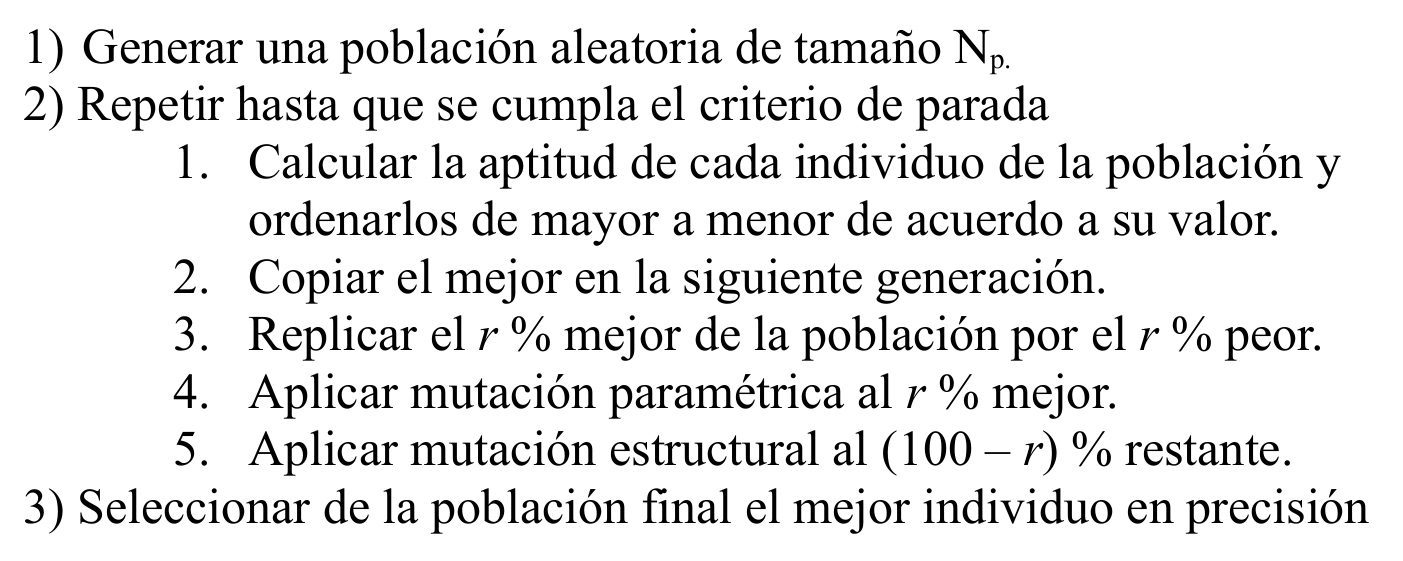
\includegraphics[keepaspectratio,width=11cm]{figuras/marcoNNEPMaeb2007.jpg}
% }
% \caption{Marco general de una variante del algoritmo CBFEP.}
% \label{CBFEPMaeb2007}
% \end{figure}
%
% Los resultados estadísticos (ver tabla IV en \cite{Hervas2007}) muestran que los modelos
% híbridos PSU no consiguen en media grandes diferencias con los modelos puros
% SU y PU, pero los mejores modelos obtenidos indican que las topologías
% híbridas son tan buenas como las mejores modelos puros, y además con un número de
% parámetros no significativamente superior (ver tabla V en \cite{Hervas2007}). En
%general,
% el número de nodos en capa oculta para un modelo híbrido es inferior o igual a los
% obtenidos por los puros (ver tabla III en \cite{Hervas2007}). Este trabajo deja abiertas
% varias cuestiones a tratar en un trabajo futuro:
% \begin{enumerate}
% 	\item A partir de las distribuciones de frecuencias asociadas a los patrones de los
% conjuntos de entrenamiento en problemas de clasificación y de las funciones de entropía
% cruzada, ¿es posible definir las características asociadas a la base de datos que
%determinen la familia de funciones (reconocedores universales) quees adecuada para
%mejorar la clasificación?
% 	\item ¿Podemos determinar algunas propiedades de las funciones de probabilidad a
% priori que permitan elegir entre diferentes familias de reconocedores universales, o
%bien
% entre la mezcla ''inteligente`` de diferentes modelos.
% 	\item ¿Es posible incorporar al algoritmo evolutivo procedimientos que permitan, en
% determinados momentos de la evolución, determinar el tipo de unidad que hay que incluir
%en
% el modelo para mejorar la precisión del clasificador en el conjunto de generalización?
% \end{enumerate}
%
% En \cite{Hervas2007a} se utiliza el mismo marco de trabajo o esquema de la figura
% \ref{CBFEPMaeb2007}, usando también modelos puros y modelos híbridos PSU. Para
% comprobar la precisión de los modelos obtenidos se usan una serie de bases de datos
% sintéticas gausianos multiclase con diferentes correlaciones lineales entre las
%variables
% de entrada y diferentes varianzas (ver sección 4 en \cite{Hervas2007a}). El método se
% compara con el análisis discriminante lineal (\textit{Linear Discriminant Analisys},
%LDA)
% \cite{Duda2000} y se ratifica
% que los modelos PSU obtienen, en la mayoría de los casos, iguales o mejores
% resultados que los modelos puros y que los obtenidos con LDA, no pudiendo éste
% último construir las funciones discriminantes en uno de los problemas, mientras que el
% modelo PSU obtiene una precisión del 100\% en generalización.
\paginavaciacompleta
		%\paginavaciacompleta
		%\chapter{Redes neuronales artificiales evolutivas multi-objetivo}\label{MOEANNs}
% \begin{quotation}
% \begin{small}
% 		\textit{El pesimista es un optimista con experiencia.}\\
% 		\textit{El pesimista es una persona previsora y bien informada.}
% \end{small}
% \begin{flushright}
% François Truffant.\\
% Anónimo.
% \end{flushright}
% \end{quotation}
\section{Algoritmos evolutivos multi-objetivo}\label{multiobjetivo}
\noindent  En ocasiones necesitamos resolver problemas con varios
objetivos a optimizar, generalmente contrapuestos, y a veces, sin  ningún  conocimiento
“a priori” de  cómo  interactúan entre sí. Son problemas de este tipo: maximizar
beneficios y minimizar costes de un producto, maximizar el desarrollo y minimizar el
consumo de gasolina de un vehículo, minimizar el peso y maximizar la fortaleza de un
componente, etc.
A estos problemas se les llama problemas de optimización multi-objetivo
(\textit{Multi-objective Optimization Problems}, MOPs) \cite{Deb2004,Coello2007}.

Mientras que en optimización mono-objetivo se busca un vector de decisión $n$-dimensional
que optimice una función escalar, en optimización multi-objetivo se intenta encontrar un
vector que optimice una función vectorial cuyos elementos representan las distintas
funciones objetivo.

A continuación definiremos qué es un MOP, así como una serie de conceptos esenciales en la
optimización multi-objetivo.
\newpage
\subsection{Optimalidad de Pareto}
\noindent
\begin{description}
\item[Definición 1. Problema de optimización multi-objetivo:] El problema de optimización
multi-objetivo se puede formular, de forma general, como el problema de encontrar el
vector
$\displaystyle \mathbf{x}^* = \left[ x^*_{1},x^*_{2},\cdots,x^*_{n}\right]^T $ que
satisfaga
las $m$ restricciones de desigualdad:
\begin{displaymath}
g_{i}(\mathbf{x})\geq0 \quad i=1,2,\cdots,m
\end{displaymath}
Las $p$ restricciones de igualdad
\begin{displaymath}
h_{i}(\mathbf{x})=0 \quad i=1,2,\cdots,p
\end{displaymath}
y que optimice
\begin{displaymath}
f(\mathbf{x})= \left[
f_{1}(\mathbf{x}),f_{2}(\mathbf{x}),\cdots,f_{k}(\mathbf{x})\right] ^T
\end{displaymath}
La solución de un MOP minimiza o maximiza (según corresponda) los componentes del vector
$f(\mathbf{x})$. Por tanto, el problema tiene $k$ objetivos y las funciones
$\displaystyle f(\cdot): \Omega \rightarrow A$ representan la correspondencia entre el
espacio
de búsqueda $\Omega$  y el espacio de las funciones objetivo $A$. De la definición de MOP
se infiere que la solución del problema puede no ser única, ya que los diversos
objetivos pueden estar en conflicto, de forma que la optimización de uno de ellos lleva,
en general, a un
descenso del valor de otro.
% De hecho, la optimización global de un problema multi-objetivo
% es un problema
% NP-completo.
\item[Definición 2. Optimalidad de Pareto:] Decimos que un punto $\mathbf{x}^* \in \Omega$
es
un óptimo de Pareto si para todo $\mathbf{x}^* \in \Omega \quad e \quad I=\left\lbrace
	1,2,\cdots,k\right\rbrace$ se verifica que $\displaystyle \forall_{i}\in I,\left(
	f_{i}\left(\mathbf{x})\right) = f_{i}\left( \vec x^*\right) \right) $ o $\exists$ $i
\in	I$ tal que $\displaystyle f_{i}(\mathbf{x})>f_{i}(\mathbf{x}^*)$.
\item[Definición 3. Dominancia de Pareto:] En un problema de minimización, un vector
$\displaystyle \mathbf{u} =\left( u_{1},u_{2},\cdots,u_{k}\right) \in A \subseteq \Re^n$
domina a otro $\displaystyle \mathbf{v} =\left( v_{1},v_{2},\cdots,v_{k}\right)$ $\in A
\subseteq \Re^n$ (denotado mediante $\displaystyle \mathbf{u} \succeq \mathbf{v}$), si y
solo si, $u$ es parcialmente menor a $v$, es decir, $\displaystyle \forall_{i} \in \left\lbrace
1,\cdots,k\right\rbrace,
\quad u_{i}\leq v_{i} \wedge \exists \quad i \in \left\lbrace 1,\cdots,k\right\rbrace
\text{ tal que } u_{i}<v_{i}$.
\item[Definición 4. Conjuntos de óptimos de Pareto:] Para un problema multi-objetivo dado
$\displaystyle \mathbf{f} (x)$, el conjunto de óptimos de Pareto $\left( \mathcal{P}^*
\right)$ se define como:
\begin{displaymath}
\mathcal{P}^*:=\left\lbrace x\in \Omega \mid \nexists  x' \in
\Omega \quad \text{tal que } \mathbf{f}\left( x'\right)  \preceq
\mathbf{f}\left(x\right)\right\rbrace
\end{displaymath}
\item[Definición 5. Frente óptimo de Pareto:] Para un problema multi-objetivo dado
$\mathbf{f}(x)$ y un conjunto de óptimos de Pareto $\mathcal{P}^*$, el frente de Pareto
$\left(
\mathcal{P}\mathcal{F}^* \right)$ se define como:
\begin{displaymath}
\left(
\mathcal{P}\mathcal{F}^* \right):=\left\lbrace \mathbf{u}=\mathbf{f}= \left( f_{1}\left(
x\right)
,\cdots,f_{k}\left( x\right)\right)  \arrowvert x \in \mathcal{P}^*\right\rbrace
\end{displaymath}
\item[Definición 6. Mínimo global de un MOP:] Dado un vector de funciones
$\displaystyle f(\cdot): \Omega \subseteq \Re^k \rightarrow \Re^n, \quad \Omega \neq 0,
\text{ y } k\geq2$, se llama al conjunto $\displaystyle \mathcal{P}\mathcal{F}^* :f(x^*)$
mínimo global, si y sólo si, $\displaystyle \forall x \in \Omega : f(x^*) \prec f(x)$,
donde $x^* \in \Omega $ se llama conjunto de soluciones de mínimo global,
$\displaystyle f(\cdot)$ es el vector de funciones objetivos y $\Omega$ el espacio de
búsqueda.

A raíz de estas definiciones se deduce que el mínimo global es la frontera de
Pareto del problema y las soluciones de mínimo global forman el conjunto de óptimos
de Pareto. Un problema de optimización de Pareto donde el espacio de búsqueda es $\Re^k$,
tiene, en general, infinitas soluciones.
\item[Definición 7. Dominancia débil y fuerte:] Un vector es un óptimo de Pareto débil si
no existe otro vector para el cual todos sus componentes en el espacio de las funciones
objetivo sean mejores. De manera formal, se puede definir como sigue:
\begin{itemize}
	\item \textbf{No dominancia débil}: Una solución $\displaystyle \mathbf{x}^* \in
\Omega $
es una solución débilmente no dominada si no existe otra solución $\displaystyle
\mathbf{x}
\in \Omega$ tal que $\displaystyle f_{i}(\vec x) < f_{i}(\mathbf{x}^*), \quad \text{para }
i=1,2,\cdots,k$.
\item \textbf{No dominancia fuerte}: Una solución $\mathbf{x}^* \in \Omega$ es una
solución fuertemente no dominada si no existe otra solución $\vec x \in \Omega $ tal que
$f_{i}(\mathbf{x}) \leq f_{i}(\mathbf{x}^*)$, para $i= 1,2,\cdots, k$ y existe al menos un
valor
$j$ para el cual $f_{j}(\mathbf{x}) < f_{j}(\mathbf{x}^*)$.
\end{itemize}
% Si un vector posee una no dominancia fuerte entonces también tiene una no dominancia
% débil,pero lo contrario no es necesariamente cierto en todas las ocasiones.
\end{description}

Así, por ejemplo, si consideramos un problema de minimización de una función de dos dimensiones
$\displaystyle f(\mathbf{x}) \in A \subseteq \Re^2$, los cuatro puntos dibujados y
señalados en la figura \ref{frente} como Frente de Pareto, son cuatro posibles soluciones al
problema. A la
hora de elegir cuál de ellos es mejor, solamente podemos decir que cualquiera de ellos es
mejor que los puntos que están fuera del frente (puntos rosas), pero que ninguno de ellos
es mejor que otro del frente. En este ejemplo se produce una minimización, de forma que
cualquier punto exterior al frente tiene al menos un valor mayor en uno de los
objetivos, y un valor mayor o igual en el otro, comparado con el valor de los
objetivos de los puntos del frente, por lo que son peores soluciones.

\begin{figure}[htb]
\centering
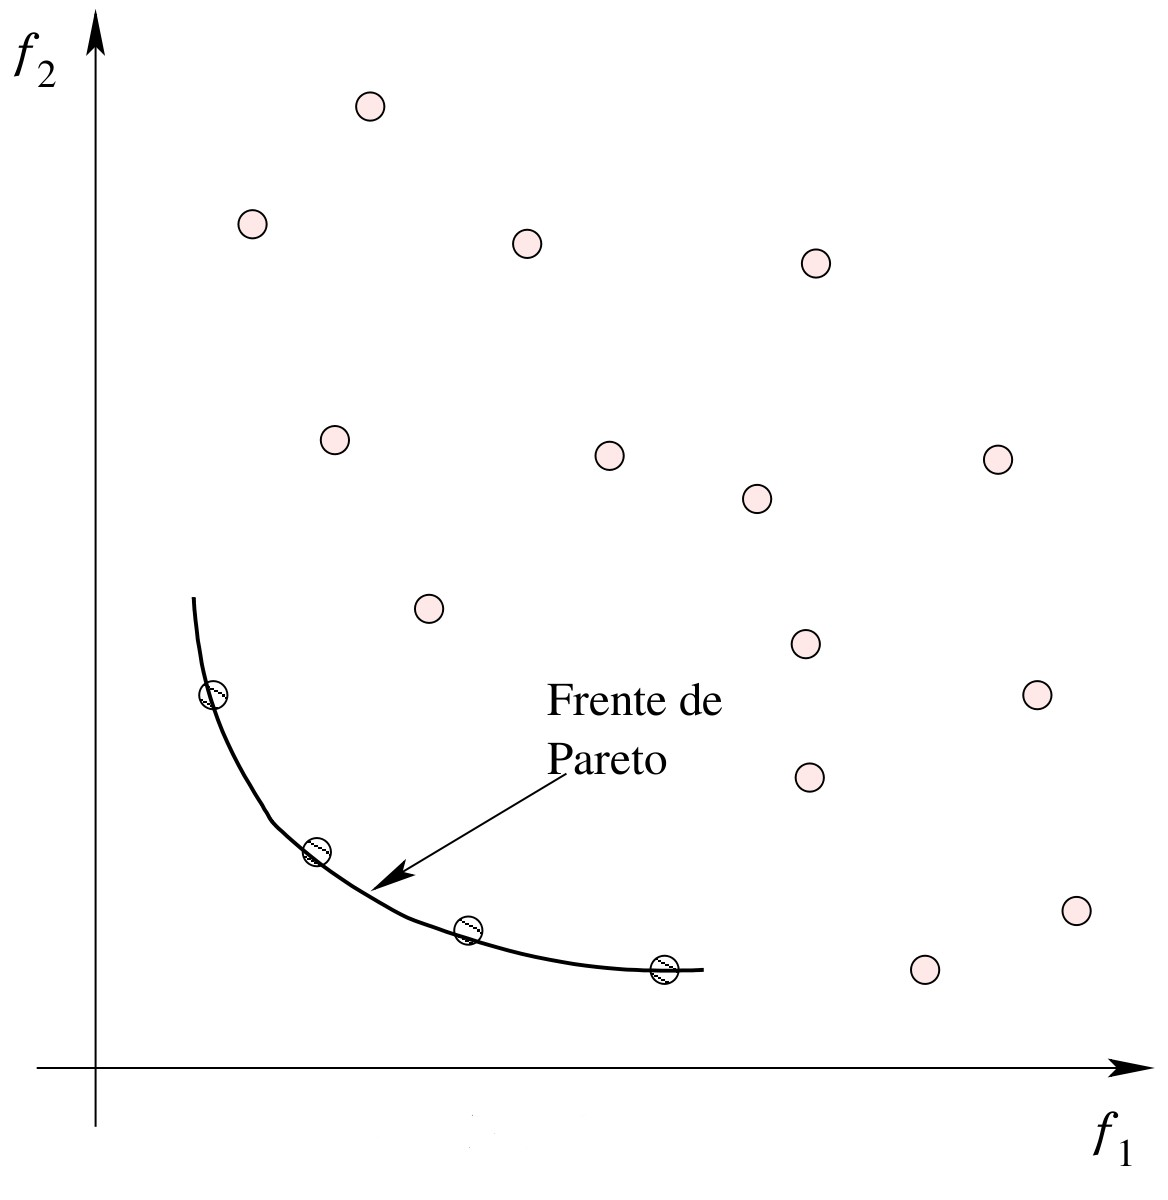
\includegraphics[keepaspectratio,width=8cm]{figuras/frentePareto.jpg}
\caption{Ejemplo de frente de Pareto con dos objetivos a minimizar.}
\label{frente}
\end{figure}

Los EAs que intentan optimizar un problema de dos o más objetivos
mediante el concepto de
optimalidad de Pareto se llaman MOEAs (\textit{Multi-Objective Evolutionary Algoritms})
\cite{Deb2004,Coello2007}, y su marco general suele ser igual que el de los EAs, es decir,
un proceso iterativo en el que evoluciona una población de individuos sujetos una serie de
operadores de selección, cruce y mutación, pero teniendo en cuenta a varias funciones
objetivo para guiar el proceso de búsqueda. Al igual que con los EAs, los MOEAs también se
pueden utilizar para el diseño de modelos de red para multiclasificación de patrones, a lo
que se le llama redes neuronales artificiales evolutivas multi-objetivo
(\textit{Multi-Objective Evolutionary Artificial Neural Networks}, MOEANNs)
\cite{Jin2006c}.

\subsection{Clasificación de MOEAs}\label{clasificacionMOEAS}
\noindent A continuación vamos a realizar una breve descripción y clasificación de los
métodos de optimización multi-objetivo más utilizados.
Concretamente, dividiremos las técnicas multi-objetivo en dos, métodos clásicos y métodos
que utilizan el concepto de óptimo de Pareto, aunque hay autores que realizan otro tipo de
clasificación. Para una revisión más completa sobre la clasificación que se muestra a
continuación ver \cite{Deb2004,Coello2007}:
\begin{description}
\item [MOEAs clásicos:] En este tipo de algoritmos no se considera el concepto
de óptimo de Pareto para la obtención de la solución final a un problema MOP, sino
que se hacen aproximaciones, no pudiéndose encontrar varias soluciones en una sola
ejecución. Por
ejemplo, estos métodos comprenden desde técnicas agregativas o con término de
regularización hasta otros métodos clásicos de
los que se hablará a continuación.
\item [MOEAs que usan el concepto de dominancia y óptimo de Pareto:] En este tipo de
algoritmos se considera el concepto de óptimo de Pareto para la obtención de la
solución final a un problema MOP, ejemplos de ellos son algoritmos como \textit{NSGAII}
\cite{Deb2002} y \textit{SPEAII} \cite{Zitzler2001}.
 \end{description}

\subsubsection{MOEAs clásicos}
\noindent Estos métodos, los cuales el lector puede consultar en
\cite{Deb2004,Coello2007}, tienden a convertir un problema multi-objetivo en otro
problema de optimización global o en un problema mono-objetivo, siendo los siguientes los métodos
más conocidos:
\begin{description}
\item [Métodos agregativos o con término de regularización:] Para
obtener la solución a un MOP basta con encontrar el mínimo o el máximo de una única
función que resume o combina todos los objetivos que se desean optimizar en uno solo. Pero
hay una serie de problemas en esta metodología. El más relevante es que se debe
proporcionar información
escalar precisa
sobre la importancia de los objetivos, a fin de evitar que uno de ellos domine a los
demás,
por lo  que  hay  que  saber  el  comportamiento  de  cada  una  de  las funciones
objetivo y tener un conocimiento “a priori” de la superficie de error. La determinación
del término de regularización adecuado para un determinado problema o factor de
aprendizaje, resulta a veces un proceso tedioso de
prueba y error. Además, solo son útiles cuando el frente de Pareto es convexo:
\begin{displaymath}
	min_{x}f_{sum}=\sum_{i=1}^k w_{i}f(\mathbf{x}) \quad x\in \Omega
\end{displaymath}
donde $\displaystyle w_{i}\geq0,\quad \sum_{i=1}^k w_{i}=1$ y $k$ el número de objetivos,
obteniéndose una sola solución en función del valor de los pesos $w_{i}$.

En el caso de ANNs en clasificación, usualmente, los objetivos a minimizar
de manera conjunta son el error
del clasificador y el número de conexiones o de nodos de los modelos de red. Así, lo que
se minimiza es el error cuadrático medio o $MSE$ (o algún otro error asociado
a la precisión del clasificador) y  se añade  un término de regularización que evite
redes
de gran tamaño. En \cite{Ludemir2006} se hace una optimización simultánea de la
estructura y los pesos de un modelo de red para generar topologías simples y con alto
porcentaje de clasificación mediante término de regularización. Los objetivos a minimizar
son la complejidad de la red y el número de patrones mal clasificados. En \cite{Jin2006b}
se estudian una serie de técnicas para trasladar la capacidad de generalización
con ANNs desde un marco multi-objetivo a uno mono-objetivo.
\item [Método de optimización minimax con pesos:] En este método se efectúa una
optimización $min-max$. Para ello se define un vector cuyos términos son las funciones
objetivo multiplicadas por diferentes pesos. El MOP se convierte en la
minimización con respecto al vector $\mathbf{x}$ del máximo valor del vector definido, para unos
pesos dados ``a priori``:
\begin{displaymath}
min\left[ max_{x\in\Omega} \left(w_{1}\cdot f_{1}(\mathbf{x}),\cdots,w_{k}\cdot
f_{k}(\mathbf{x})\right)
\right]
\end{displaymath}

Otra variación de este método se produce al fijar un vector constante que se resta al
vector de funciones objetivo, de forma que la formulación del problema queda:
\begin{displaymath}
min\left[ max_{x\in \Omega}\left(w_{1} \cdot
\left(f_{1}(\mathbf{x})-\gamma_{1}\right),\cdots,w_{k} \cdot
\left(f_{k}(\mathbf{x})-\gamma_{k}\right)\right) \right]
\end{displaymath}
\item [Método de permutación $\epsilon$:] Este método reduce un MOP a un problema
mono-objetivo con restricciones, y sirve para obtener aproximaciones en frentes convexos y
no convexos. Se basa en la minimización de una función objetivo principal y  considera  los
demás objetivos como restricciones acotadas por ciertos  niveles permisibles  $\varepsilon_{i}$
, efectuándose una minimización con un solo objetivo para la función objetivo más
relevante, sujeta a restricciones adicionales en las otras funciones objetivo:
\begin{gather} \nonumber
min_{x}f_{k}(x) \\ \nonumber
\text{sujeto a} \quad  f_{i}(x)\leq\epsilon_{i} \quad \forall i\neq k \\ \nonumber
x \in \Omega \nonumber
\end{gather}
\item [Métodos de las métricas ponderadas:] En estos métodos se considera un punto
utópico o solución ideal $f^*$, a la que se desea llegar mediante la minimización de una
función objetivo a través de una determinada métrica, como puede ser la distancia euclídea
o la métrica de \textit{Tchebycheff} \cite{Karlin1966}.
\begin{displaymath}
min \left( \sum_{i=1}^k w_{i}	\parallel f^*-f(x)\parallel^\rho\right) ^{(1/\rho)}, \quad
{x\in\Omega}
\end{displaymath}
donde $\rho$ puede tomar valores entre $\left[ 1,\infty\right]$.
\item [Programación por metas:] La idea principal de la programación por metas es
encontrar soluciones que logren un objetivo predefinido para una o más funciones
objetivo. Si la solución al objetivo predefinida no existe, el propósito es minimizar las
desviaciones de todos los objetivos.
Si consideramos una función objetivo $f(x)$, y un valor $t$ para cada objetivo de diseño,
la solución es encontrar el objetivo que alcance el valor $t$, sujeto a que debe ser una
solución factible:
\begin{displaymath}
 \text{objetivo} \quad f(x)=t, \quad x\in\Omega
\end{displaymath}
% Si el valor $t$ es más pequeño que la solución óptima $f(x^*)$ no existe solución
% factible que alcanze el objetivo exacto, por tanto se intentaría encontrar la solución
% que minimice la desviación entre el objetivo alcanzado y el deseado, $f(x^*)-t$. Si el
% valor $t$ es mayor, la solución al problema es $x$,
\item [Soluciones óptimas lexicográficas:] Este método convierte el problema de
optimización de Pareto, donde todas las componentes del vector de funciones $f(\cdot)$
tienen la misma importancia, en un problema donde las componentes de dicho vector tienen
una importancia decreciente. Así, el problema de optimización lexicográfica se formula
como una secuencia de $k$ minimizaciones $P_{i}$ de tipo:
\begin{gather} \nonumber
min_{x\in\Omega} f_{k}(x)\\ \nonumber
\text{sujeto a} \quad f_{i}(x)\leq\alpha_{i}, \quad i=1,\cdots,k-1 \nonumber
\end{gather}
\end{description}

Los métodos clásicos, generalmente, no suelen ser eficaces debido a:
\begin{enumerate}
\item Sólo dan un punto del frente de Pareto como solución, siendo
necesaria la repetición del algoritmo un gran número de veces para obtener todas las
soluciones.
\item Muchos de estos algoritmos necesitan un conocimiento previo del problema para
ser viables. Es el caso del valor de las funciones de peso o del punto utópico u óptimo.
\item Alguno de estos algoritmos son muy sensibles a la forma del frente de Pareto.
\item Estos algoritmos no son válidos en problemas con incertidumbre o en problemas
estocásticos.
\item Los algoritmos de optimización clásicos no son válidos para resolver problemas de
un sólo objetivo con un espacio de búsqueda discreto, luego tampoco lo son para resolver
MOPs con espacio de búsqueda discreto.
\end{enumerate}

\subsubsection{MOEAs que usan el concepto de dominancia y óptimo de Pareto}
\noindent Los algoritmos que utilizan el concepto de óptimo de Pareto para obtener un
conjunto de soluciones, que representan un compromiso entre los distintos objetivos a
optimizar, se pueden dividir, de forma general, en métodos no elitistas y elitistas, o
en
métodos de primera generación y de segunda generación respectivamente. Se entiende por
método elitista aquel que utiliza de una manera u otra al mejor o mejores individuos de
una población para avanzar en el proceso de evolución, mientras que los métodos no
elitistas no suelen retener las mejores soluciones de una generación a otra, o formar
conjuntos externos de mejores soluciones que sustituyan a individuos de la población en
determinados momentos de la evolución.

A continuación solo se hará referencia a los MOEAs más populares en la literatura que usan
el concepto de óptimo de Pareto, dejando al lector la
consulta de \cite{Deb2004,Coello2007} para obtener una descripción más detallada y amplia
de éstos y de otros algoritmos.
\begin{description}
	\item[Métodos no elitistas:] Estos métodos no utilizan operadores que ayuden a
preservar la elite de individuos dentro de una población, con lo que si se obtiene una
buena solución en generaciones tempranas de un EA, ésta puede que no llegue al final de
la evolución si no se realizan los procesos de selección, cruce y mutación oportunos.
Tienen la ventaja de que son fáciles de entender y sencillos de implementar, y algunos de
ellos convergen bien y encuentran un conjunto de soluciones de Pareto bien distribuidas y
diversas. Ejemplos de estos algoritmos son VEGA (\textit{Vector Evaluated Genetic
Algorithm}, MOGA (\textit{Multiple Objective Genetic Algorithm}), NSGA
(\textit{Non-Dominated Sorting Genetic Algorithm}), NPGA (\textit{Niched-Pareto Genetic
Algorithm}), HLGA (\textit{Hajela and Lins Genetic Algorithm}), MSGA (\textit{Multisexual
Genetic Algoritm}) y PESA (\textit{Pareto Envelope-based Selection Algorithm}).

\item[Métodos elitistas:] Este tipo de algoritmos usan operadores para preservar la
diversidad y los mejores individuos de una generación a otra. Por norma
general, obtienen mejores soluciones que los algoritmos de primera generación, ya que
la probabilidad de que la población de hijos mejore de una generación a otra mediante
operadores de selección, cruce y mutación adecuados es mayor (se suele
mantener una población secundaria).

Existen muchas formas de implementar el elitismo, por ejemplo,
guardando el mejor individuo de la población o cruzando padres y uniéndolos a la población
hija, escogiendo los $N$ mejores individuos. La elección del número de
individuos de elite que deben pasar de una generación a otra es importante, pues si
este número es grande disminuirá la diversidad de la población, lo que se conoce como presión
selectiva. Se podría pensar que en los algoritmos no elitistas
también se podrían conservar los mejores individuos de una generación para incluirlos en
la siguiente, pero en ese caso no estaríamos teniendo en cuenta el concepto de Pareto, y
sería difícil identificar qué soluciones son las que tienen un mejor compromiso entre los
objetivos que
perseguimos. Ejemplos de algoritmos elitistas son: NSGAII (\textit{Non-Dominated Sorting
Genetic Algorithm 2}), PAES (\textit{Pareto-Archived Evolution Strategy}), SPEA
(\textit{Strength Pareto Evolutionary Algorithm}), SPEAII (\textit{Strength
Pareto Evolutionary Algorithm 2}), PESAII (\textit{Pareto Envelope-based Selection
Algorithm 2}), $\mu \text{GA}$ (\textit{micro Genetic Algorithm}), parEGO (\textit{Pareto
Efficient Global Optimization}), $\epsilon\text{-MOEA}$ (\textit{epsilon} MOEA), MOMGA
(\textit{Multi-Objective Messy Genetic Algorithm}), PDE (\textit{Pareto Differential
Evolution}) y MOEAs con utilización de restricciones.
\end{description}

\section{Medidas $(MS,C)$ en redes neuronales artificiales}\label{objetivosRedes}
\noindent La utilización de la precisión, $C$ y la mínima sensibilidad, $MS$, en el
diseño de modelos de ANNs para problemas de clasificación multi-clase es novedoso.
%, a
%pesar de que estos dos objetivos sean subconjuntos de la superficie formada por
%los $Q(Q-1)$  puntos exteriores a la diagonal principal de la matriz de confusión.
Habitualmente lo que se pretende optimizar cuando se utilizan modelos de red para
clasificación de patrones en problemas multi-objetivo es la precisión y la complejidad de
la red \cite{Goh2008,Dehuri2009,Jin2005}, ésta última definida mediante alguna de las
siguientes formas:
\begin{description}
\item[Complejidad gaussiana o \textit{Weight Decay}:] La complejidad se define como la
suma de los pesos al cuadrado de cada una de las conexiones de la red dividido por dos.
\begin{displaymath}
\Omega(R)=\frac{1}{2}\sum_{k} W_{k}^2
\end{displaymath}
siendo $W_{k}$ el valor del peso $k$-ésimo de la red $R$. Tiene la desventaja de que no
es
capaz de llevar los pesos pequeños e irrelevantes a cero cuando se utilizan algoritmos
de	aprendizaje basados en gradiente.
\item[Complejidad de Laplace:] Es una alternativa al método anterior para llevar a
cero los pesos irrelevantes, y se define como la suma en valor absoluto de los valores de
los pesos:
\begin{displaymath}
\Omega(R)=\sum_{k} \arrowvert W_{k}\arrowvert
\end{displaymath}
\item[Número de enlaces de la red:] El número total de enlaces de una red como medida
de complejidad tiene una naturaleza discreta, por lo que es un buen
método para usarlo en optimización evolutiva, pero no es bueno aplicarlo a métodos
basados en gradiente. Se define como la suma de cada uno de los enlaces existentes en
la red:
\begin{displaymath}
\Omega(R)=\sum_{i}\sum_{j} \arrowvert lk_{ij}\arrowvert
\end{displaymath}
siendo $lk_{ij}$ el peso que va desde una neurona $i$ de la capa oculta a una neurona $j$
de la capa de entrada.
\item[Número de neuronas en la capa/s oculta/s de la red:] Similar al método anterior,
pero en esta ocasión se realiza una suma del número de neuronas que existan en la capa
o capas ocultas de una determinada red.
\begin{displaymath}
\Omega(R)=\sum_{i}\sum_{j}h_{ij}
\end{displaymath}
siendo $h_{ij}$ la neurona número $j$ de la capa oculta $i$.
\end{description}

Existen trabajos y estudios para la clasificación de patrones biclase que utilizan la
precisión y la sensibilidad como medidas de rendimiento \cite{Jin2006b},
utilizando o no ANNs. Concretamente se utiliza la maximización de la
sensibilidad o $TPR$ y la minimización del $FPR$, o de otra manera, $TPR$ y $Sp$
$\left(1-FPR\right)$, como objetivos a maximizar. En \cite{AlbertoF2009}, la métrica
seleccionada es la media geométrica de los porcentajes positivos, midiendo de esta manera
un rendimiento más balanceado que usando solamente la precisión global. Pero el
concepto de sensibilidad que se usa en la mayoría de este tipo de trabajos solo sirve para
problemas binarios y no para multiclase.

\section{Trabajos con MOEANNs}
\noindent Tradicionalmente, como acabamos de comentar, en el diseño de ANNs mediante MOEAs
se suelen establecer dos objetivos a optimizar, el error en entrenamiento y la complejidad
de la red. Por ejemplo, Abbass \cite{Abbass2001,Abbass2003}, el principal exponente en
este aspecto, ha presentado diferentes estudios sobre el diseño y entrenamiento de ANNs
para clasificación y regresión, usando precisión y complejidad como objetivos en MOEAs.
Abbass establece un marco general para evolución multi-objetivo de ANNs basado en
DE (\textit{Differential Evolution}) \cite{Price2005} (ver capítulo \ref{diferencial}), donde se
evoluciona conjuntamente, para cada red, la estructura y los pesos, y se aplican operadores de cruce
y mutación, basados en la selección aleatoria (sin repetición) de tres padres de la población.

En cuanto a aplicaciones de MOEAS para el entrenamiento de ANNs cabe destacar el
reconocimiento de imágenes propuesto en \cite{Wiegand2004}, donde se detectan y clasifican rostros
humanos mediante MOEANNs usando el algoritmo NSGAII e introduciendo una LS en cada generación de
la evolución. Los objetivos a optimizar son el $MSE$ y el número de neuronas en capa
oculta. Algunos artículos y variaciones encaminadas en la misma dirección que el citado
trabajo se pueden consultar en \cite{Roth2006,Gepperth2006}.

Yauchu Jin, en varios de sus artículos \cite{Jin2004,Jin2005,Jin2006} hace un estudio de
los resultados obtenidos con el algoritmo NSGAII, comparándolo con otros MOEAs y con
algoritmos mono-objetivo con término de regularización para ANNs. Se usan como objetivos la
minimización del $MSE$ y la complejidad de la red, y también emplea versiones híbridas con
algoritmos de LS como el \textit{Resilient Backpropagation} (Rprop) \cite{Riedmiller1993}.

En \cite{Jin2006b} se pueden estudiar algunas técnicas y heurísticas para obtener el
frente de Pareto. Se basan no solo en entrenar redes aplicando el conjunto de
entrenamiento a modelos de red a lo largo del proceso evolutivo, para finalmente
aplicar el conjunto de generalización, sino que se basan también en determinados ajustes
sobre los datos de entrenamiento, como por ejemplo: la adición de ruido gaussiano, que
consiste en la adición a los datos del conjunto de entrenamiento de un ruido
gaussiano cada cierto número de generaciones, o la adición de ruido a través de
medias, que consiste en la adición a los datos del conjunto de entrenamiento de un
ruido partiendo de valor medio de cada entrada.

Otros trabajos \cite{Fieldsend2002,Fieldsend2005} utilizan otras técnicas sobre los
conjuntos de entrenamiento para mejorar la capacidad de generalización cuando se obtiene
el frente de
Pareto, proponiendo un determinado MOEA, dependiendo de si en la obtención del frente se
utiliza: a) el conjunto de entrenamiento, b) los conjuntos de entrenamiento y validación
o c) el conjunto de entrenamiento con técnicas de \textit{bootstraping} (muestreo con
reemplazamiento) \cite{Bootstrapping2006} para prevenir el
sobre ajuste en entrenamiento.

Otros autores como M. Delgado y colaboradores, utilizan modelos de clasificación utilizando ANNs
recurrentes para el entrenamiento y obtención de modelos de red. Así, en
\cite{Delgado2005} se utiliza una
mejora del algoritmo SPEA en problemas de inferencia gramatical, donde se optimizan tres
objetivos: maximizar el número de aprendizajes positivos en entrenamiento, minimizar el
error cometido, y minimizar el número de neuronas en la red. La codificación es directa,
empleando cruce y mutación para la obtención de nuevos hijos. En \cite{Delgado2007} se
utilizan redes recurrentes dinámicas con una versión híbrida de SPEAII, intentando
minimizar el $MSE$ y el número de neuronas en capa oculta, utilizando un algoritmo de LS
basado en gradiente. Como operadores se utiliza tanto cruce como mutación.

En \cite{Gonzalez2003} se aplican varios operadores de cruce y mutación basados en las
transformaciones de matrices SVD (\textit{Singular Value Descomposition}) y OLS
(\textit{Orthogonal Least Squares}), que producen modificaciones locales y globales en
redes RBF. Los objetivos a optimizar
son el $MSE$ y la complejidad de la red, utilizando el procedimiento de orden
del algoritmo MOGA y aplicándole el método de Levenverg-Maquart \cite{Marquardt1963} como
algoritmo de LS. Un criterio parecido se utiliza en \cite{Hatanaka2006}, pero en este caso
el MOEA aplicado es NSGAII.

En \cite{Yen2006} se propone una forma de asignación de aptitud basada en la densidad de
orden en un algoritmo llamado HRDGA (\textit{Hieralchical Rank Density Genetic
Algorithm}). Se convierten múltiples objetivos de alta dimensionalidad en dos, complejidad
de la red y error cometido, minimizando el error de orden de un individuo en concreto y el
valor de densidad de la población. Los individuos del frente de Pareto se buscan por medio
de esquemas de difusión y elitismo, y se previene la introducción de individuos dañados
mediante el concepto de región perdida.

Existe otro buen número de trabajos relacionados con MOEAs para el entrenamiento de ANNs,
pero entendemos que este no es el objetivo principal de este trabajo de tesis. El lector
puede consultar un estado del arte más amplio en \cite{Ou2007,Goh2008,Jin2008}.

Abordamos a continuación el algoritmo MPENSGAII, como propuesta fundamental y uno de los
objetivos de este trabajo de tesis.

\section{El algoritmo MPENSGAII}\label{algoritmo}
\noindent A partir de ahora se utilizarán términos y se hará referencia a
metodologías y expresiones formales explicadas y detalladas en los capítulos
\ref{medidasRendimiento} y \ref{redesneuronales}
de esta tesis. En esta sección exponemos  MPENSGAII (\textit{Memetic Pareto
NSGAII}) \cite{Fernandez2010}, un MOEA para la obtención de modelos de ANNs para
multi-clasificación de patrones, utilizando como modelo funcional unidades de base
sigmoides (SUs), ya introducidas en la sección \ref{unidadesSigmoide} del
capítulo \ref{redesneuronales}, y usando un algoritmo de LS para mejorar la capacidad de
generalización de los multiclasificadores y el proceso de aprendizaje.

MPENSGAII se basa en NSGAII \cite{Deb2002}, utilizando como características más
representativas el ordenamiento rápido de no-dominados para la obtención
del frente de Pareto, el cálculo de la distancia \textit{crowding} para el mantenimiento
de la diversidad, y la selección por torneo binario. En esta sección no explicaremos este
tipo de operadores y técnicas al considerarlo repetitivo, ya que siguen la misma filosofía
usada en NSGAII, dejando al lector una descripción detallada sobre ello en \cite{Deb2002}.

MPENSGAII obtiene diferentes conjuntos de clasificadores
no dominados que presentan un buen balanceo entre $C$ y $MS$ (ver capítulo
\ref{medidasRendimiento}), que son los dos objetivos a optimizar. El
ordenamiento rápido de no dominados utiliza como medidas para determinar la no dominancia
de un individuo, dos funciones objetivo que miden la precisión del mismo, y que se
detallan en la siguiente sección.

MPENSGAII estima los parámetros y la estructura de la red de manera simultanea. La
población de individuos está sujeta a operaciones de replicación y de mutación, no
usando operador de cruce, por las mismas razones que en el algoritmo CBFEP del capítulo
\ref{evoMonoObjetivo}. En cuanto a la codificación de los modelos de red, se sigue la
misma codificación explicada en el algoritmo CBFEP, pero aplicado solo a ANNs con SUs, en
vez de a modelos híbridos.

\subsection{Funciones objetivo}\label{funcionesObjetivo}
%Aqui iba lo primero que he puesto en trabajos previos con MOEANNS
\noindent Si asumimos que todos los errores de clasificación son igualmente costosos y que
no hay preferencia ni penalización para una determinada clase de patrones, un buen
clasificador debería obtener un alto nivel de precisión global, así como un
aceptable nivel de clasificación para cada clase de un problema. En
problemas reales, estos objetivos suelen estar en conflicto (ver sección \ref{propiedades}
del capítulo \ref{medidasRendimiento}), por tanto la aplicación de un MOEA para la
resolución de este problema es una buena opción. Teniendo en cuesta ésto, las dos
funciones objetivo a optimizar con MPENSGAII son:
\begin{itemize}
\item La mínima sensibilidad de todas las clases del problema, $MS$:
\begin{displaymath}
A_{1}\left( g,\mathbf{\Theta}\right) = MS(g)
\end{displaymath}
\item La entropía cruzada, $E$, como medida de error global, (al igual que con el algoritmo
CBFEP), ya que aunque depende del conjunto de datos, se ha demostrado que, por norma
general, $E$ converge mejor que $C$ (ver sección \ref{etapas} del capítulo
\ref{evoMonoObjetivo}). Concretamente, como función de aptitud a la hora de
evaluar un individuo se usará la siguiente expresión:
\begin{displaymath}
\label{aptitudNNEP}
A_{2}\left( g,\mathbf{\Theta}\right) =\frac{1}{1+E\left( g,\mathbf{\Theta}\right)}
\end{displaymath}
es decir, maximizar una transformación estrictamente decreciente de $E$.
\end{itemize}

Para asignar una clase a una nueva observación se sigue el esquema ``1 de $Q$''
explicado en el algoritmo CBFEP.

En \cite{Fernandez2009a} se puede estudiar una variante de MPENSGAII en la que
utilizamos los siguientes objetivos:
\begin{itemize}
\item Minimizar el coeficiente de variación de las sensibilidades (\textit{Variation
Coefficient}, VC):
\begin{displaymath}
A_{1}=VC=\frac{\sqrt{\frac{\sum_{i=1}^{Q}(S_{i}-\bar{S})^2}{Q-1}}}{\bar{S}}
\end{displaymath}
siendo $\bar{S}$ la media de las sensibilidades de cada clase $S_{i}$.
\item Como segunda función objetivo emplea $E$, es decir, la función
objetivo $A_{2}$ de MPENSGAII.
\end{itemize}

En esta variante comparamos con algoritmos, como el algoritmo MPANN \cite{Abbass2003} y
con un
evolutivo en dos etapas llamado E+A \cite{Martinez-Estudillo2008} (ver sección \ref{balanceados} del
capítulo \ref{medidasRendimiento}), presentando buenos resultados en una serie conjuntos de datos
obtenidos de la UCI \cite{UCI2007}. La metodología seguida es similar a la de MPENSGAII,
pero solo cogiendo la parte superior del frente de Pareto, la que proporciona el mejor
individuo en $E$, y no los dos extremos como veremos en las siguientes secciones.
Esto nos permitió poder comparar con los algoritmos antes mencionados.
\newpage
\subsection{Operadores}\label{operadoresMPENSGAII}
\noindent Los operadores utilizados  en cuanto a mutación son prácticamente los mismos que
los utilizados con CBFEP.

Hay 4 mutaciones estructurales: Añadir neurona, AN, eliminar neurona,
DN, añadir enlace, AL y eliminar enlace, DL. Se realizan de la misma forma que con el
algoritmo CBFEP, pero en este caso, al utilizar solo SUs como unidades de base, no es
necesario elegir el tipo de unidad a introducir en capa oculta.

La mutación paramétrica sí cambia con respecto CBFEP, puesto que se aplica a cada uno de
los pesos de la red, añadiéndoles un ruido gaussiano dado por:
\begin{gather} \nonumber
w_{ij}(t+1) = w_{ij}(t)+\xi_{1}(t)\\ \nonumber
\theta_j(t+1) = \theta_{j}(t)+\xi_{2}(t)\\ \nonumber
\beta_{ij}(t+1) = \beta_{ij}(t)+\xi_{3}(t) \nonumber
\end{gather}
donde $\xi_{1}(t)$, $\xi_{2}(t)$ y $\xi_{3}(t)$ son variables aleatorias normales
$N(0,T(t))$, donde $T(t)$ representa la temperatura en la generación $t$ a lo largo de la
evolución (el valor de $T(t)$ disminuye produciéndose descensos más drásticos al comienzo
de la evolución (exploración), y más lentos al final (explotación). La temperatura $T$ en
en la generación $t$ viene dada por:
\[
T(t)=
\begin{cases}
r \cdot T(t-1) & \text{ si } t=kI,k=1,2,\cdots,\frac{I_{max}}{I_{t}}\\
T(t) & \text{en los restantes casos}
\end{cases}
\]
donde $r$ es el factor de descenso, $I_{t}$ el número de
generaciones que deben transcurrir para que se actualice el valor de la temperatura e, $I_{max}$ es
el número máximo de generaciones que se ejecutará MPENSGAII.

A cada individuo de la población se le aplica aleatoriamente una y solo una de las 5
mutaciones utilizadas. Si alguna mutación no tiene éxito por alguna restricción especial
referida a la arquitectura de la red (ver mutaciones del algoritmo CBFEP), se
elige otra mutación aleatoriamente.

Las mutaciones AL y DL se aplican solamente en capa oculta y capa de salida, mientras que
las mutaciones AN y DN se realizan en capa oculta. El número de neuronas a añadir o
eliminar se elije aleatoriamente entre los valores $\left[1,2\right] $, mientras que el
número de enlaces a añadir o eliminar depende de los que haya en ese momento en cada red.
Se añadirán o eliminan el 30\% del total de enlaces que haya entre capa de entrada y capa
oculta y el 5\% del total de los enlaces existentes entre capa oculta y capa de salida.
Con respecto al valor de los pesos que se añaden en los enlaces, se toman valores entre
$\left[-5,5\right] $ para la capa entrada-oculta y $\left[ -10,10\right] $ para la capa
oculta-salida.

\subsection{iRprop+ como búsqueda local}\label{rprop}
\noindent Una mejora dentro de los EAs, tanto para algoritmos mono-objetivo como
multi-objetivo, es la incorporación de procedimientos de LS a través de la evolución
\cite{Cotta2001,Grosan2007,Goh2009}. Algunos estudios llevados a cabo sobre el proceso de
convergencia de un EA, muestran como éste encuentra rápidamente soluciones aceptables a un
problema, sin embargo y por regla general, se necesitan más generaciones para alcanzar una
buena solución \cite{Houck1997} que si se utiliza un algoritmo basado en gradiente. Por
otro lado, los algoritmos de LS pueden quedar atrapados en un óptimo local, aunque en
ocasiones pueden encontrar el óptimo global cuando la búsqueda se lleva a cabo en pequeñas
regiones del espacio. De esta forma, en combinación con EAs, los algoritmos de LS
proporcionan un método para obtener de manera rápida y eficiente buenas soluciones
a un problema \cite{Smith2007}.

Una vez dicho esto, MPENSGAII se ha mejorado mediante la implementación de un algoritmo de
LS adaptado a nuestra codificación y a nuestras funciones objetivo, concretamente el
algoritmo iRprop+ (\textit{Improved Resilient Back-propagation}) \cite{Igel2003}, que es
una mejora del original Rprop \cite{Riedmiller1993}. El algoritmo Rprop (\textit{Resilient
Back-propagation}) \cite{Riedmiller1993}, como método de LS, es una de las mejores
técnicas conocidas en este aspecto en términos de velocidad de convergencia, precisión y
robustez con respecto a sus parámetros. iRprop+ es un procedimiento basado
en gradiente, difiriendo de las técnicas clásicas de propagación hacia atrás del error en
que, las derivadas parciales de la función error, sólo se usan para determinar el
sentido en que se deben corregir los pesos de la red, pero no las magnitudes de los
ajustes. El modelo de actualización de cada peso $ij$ de una ANN viene dado por
$\displaystyle
w_{ij}^{(t+1)}=w_{ij}^{(t+1)}+\bigtriangleup w_{ij}^{(t+1)}$, donde
$\bigtriangleup w_{ij}^{(t+1)}$ se estima con una función de cambio de signo de la
derivada del error entre las iteraciones $(t)$ y $(t-1)$, y en función del tamaño de paso
para los pesos $\bigtriangleup _{ij}$, tal como se realiza tradicionalmente con las
técnicas basadas en
gradiente. Así, si el signo de la derivada no cambia en las dos últimas iteraciones, el
tamaño de paso se aumenta. Si la derivada es cero no se modifica y si cambia de signo
se disminuye. iRprop+ aplica una estrategia de \textit{backtracking} para decidir la
dirección de corrección del valor de los pesos de la red, concretamente la idea es que la
actualización de los pesos depende de la evolución del error. De esta manera, el esquema
de entrenamiento combina información local con información global (por ejemplo, el valor
del error en cada iteración) a la hora de decidir si debe modificar los pesos. Un cambio
de signo en una derivada parcial significa que se ha saltado un mínimo local. Se ha
demostrado mediante problemas de prueba o \textit{benchmarks} \cite{Igel2003}, que
iRprop+ consigue mayor rendimiento que su versión original.

En este trabajo usamos iRprop+ cuando combinamos la población de padres
e hijos en
MPENSGAII (paso 8-d de la figura \ref{marcoMPENSGAII}). Entonces, solo los individuos del
primer frente de Pareto (obtenido mediante una ordenación rápida de los individuos no
dominados) de
la población combinada se optimizan mediante el algoritmo iRprop+. El coste
computacional
asociado a este tipo de operaciones se reduce considerablemente en nuestro MPENSGAII, ya
que no aplicamos la LS a todos los individuos mutados de la población de
descendientes, ni en todas las generaciones. El procedimiento de LS se aplica sólo al
principio (2/7 del número total de generaciones), en la mitad del proceso evolutivo (4/7)
y al final (6/7) del mismo; mientras que en otros trabajos \cite{Jin2008} se usa la
LS en cada generación, y en la mayoría de las ocasiones a todos los
individuos de la población.

iRprop+ solo se ha aplicado en una dirección de las dos funciones objetivo, ya que $MS$,
en general, no es derivable. Concretamente se ha aplicado en la dirección de $E$. Así,
hemos llevado a cabo una adaptación del algoritmo a la función de activación
\textit{softmax} y a la función de
entropía cruzada, $E$ (normalmente, en la literatura específica, iRprop+ se ha utilizado con el
$MSE$), de forma que el vector
gradiente viene dado por:
\begin{gather} \nonumber
\bigtriangledown E(\mathbf{\beta}^q , \mathbf{w})=\left( \frac{\partial
E}{\partial{\mathbf{\beta}^q}},\frac{\partial E}{ \mathbf{w} }\right)
\end{gather}
donde $\mathbf{\beta}^q,\mathbf{w}$ son los vectores de parámetros asociados a una red
neuronal.

Sea $\Theta_{q}$ cualquiera de los parámetros de $\mathbf{\beta}^q$ y $\mathbf{w}$,
entonces
\begin{gather} \nonumber
\frac{\partial E}{\partial \mathbf{\Theta}_{q}}=\frac{1}{N}\sum_{n=1}^N \sum_{q=1}^Q
y_{n}^q \frac{1}{g_{q}\left( \mathbf{x}_{n},\Theta_{q}\right)}  \frac{\partial g_{q}
\left(\mathbf{x}_{n} ,\mathbf{\Theta}_{q}\right)} {\partial \mathbf{\Theta}_{q}}
\end{gather}

\begin{small}
\begin{gather} \nonumber
\frac{\partial g_{q}
\left(\mathbf{x}_{n} ,\mathbf{\Theta}_{q}\right)} {\partial \mathbf{\Theta}_{q}} =
\frac{1}{\left( 1+\sum_{q=1}^{Q-1} e ^{f_{q}}\right)^2}\left\lbrace e ^{f_{q}}
\frac{\partial f_{q}}{\partial \mathbf{\Theta}_{q}}\left(1+\sum_{q=1}^{Q-1} e
^{f_{q}}\right)-e^{f_{q}}\sum_{q=1}^{Q-1} e^{f_{q}} \frac{\partial f_{q}}{\partial
\mathbf{\Theta}_{q}} \right\rbrace
\end{gather}
\end{small}

\begin{gather} \nonumber
\frac{\partial g_{q}\left(\mathbf{x}_{n} ,\mathbf{\Theta}_{q}\right)} {\partial
\mathbf{\Theta}_{q}} = g_{q}\frac{\partial f_{q}}{\partial\mathbf{\Theta}_{q}} - g_{q}^2
e^{-f_{q}} \sum_{q=1}^{Q-1} e^{f_{q}} \frac{\partial
f_{q}}{\partial\mathbf{\Theta}_{q}}
\end{gather}

Finalmente, para la capa de salida de cada ANN se tiene que
\begin{equation*}
	\frac{\partial f_{q}}{\partial \beta_{0}^k}=\delta_{kq}=
	\begin{cases}
		0 & k\neq q \\
		1 & k=q
	\end{cases}, \quad
	\frac{\partial f_{q}}{\partial \beta_{s}^k}=
	\begin{cases}
	0 & q\neq k \\
	\mathbf{\sigma}\left( \sum_{i=1}^k w_{is}x_{i}\right)  & q=k
	\end{cases}
\end{equation*}

y para la capa de salida que
\begin{displaymath}
\frac{\partial f_{q}}{\partial w_{s}^t} = \mathbf{\beta}_{s}^q \mathbf{\sigma}'\left(
\sum_{i=1}^k w_{is}x_{i}\right) x_{t},\quad \text{donde} \quad
s=1,2,\cdots,m;t=1,2,\cdots,k
\end{displaymath}

En un trabajo futuro, quedaría abierta la opción de aplicar un algoritmo de LS en las dos
direcciones u objetivos que guían a MPENSGAII (ver artículos
de Moller \cite{Moller1993,Falas2005}), por ejemplo mediante el uso de otra función
objetivo que sustituya a $MS$ y que sea derivable, mediante un procedimiento por etapas en
las que de forma alternada o secuencial se optimicen los objetivos del problema, o
mediante algún tipo de combinación que utilice información de los dos objetivos.

\subsection{Etapas y aspectos relevantes de MPENSGAII}\label{etapas}
\noindent Una vez descritos los operadores de mutación a aplicar, los objetivos a
optimizar, y el método de LS, pasamos a comentar los aspectos más relevantes del algoritmo
MPENSGAII. El marco general de MPENSGAII se muestra en la figura \ref{marcoMPENSGAII}, y
un esquema de las etapas o pasos de MPENSGAII se encuentra en la figura
\ref{etapasMPENSGAII}.

\begin{figure}[!htp]
\centering
\fbox{
	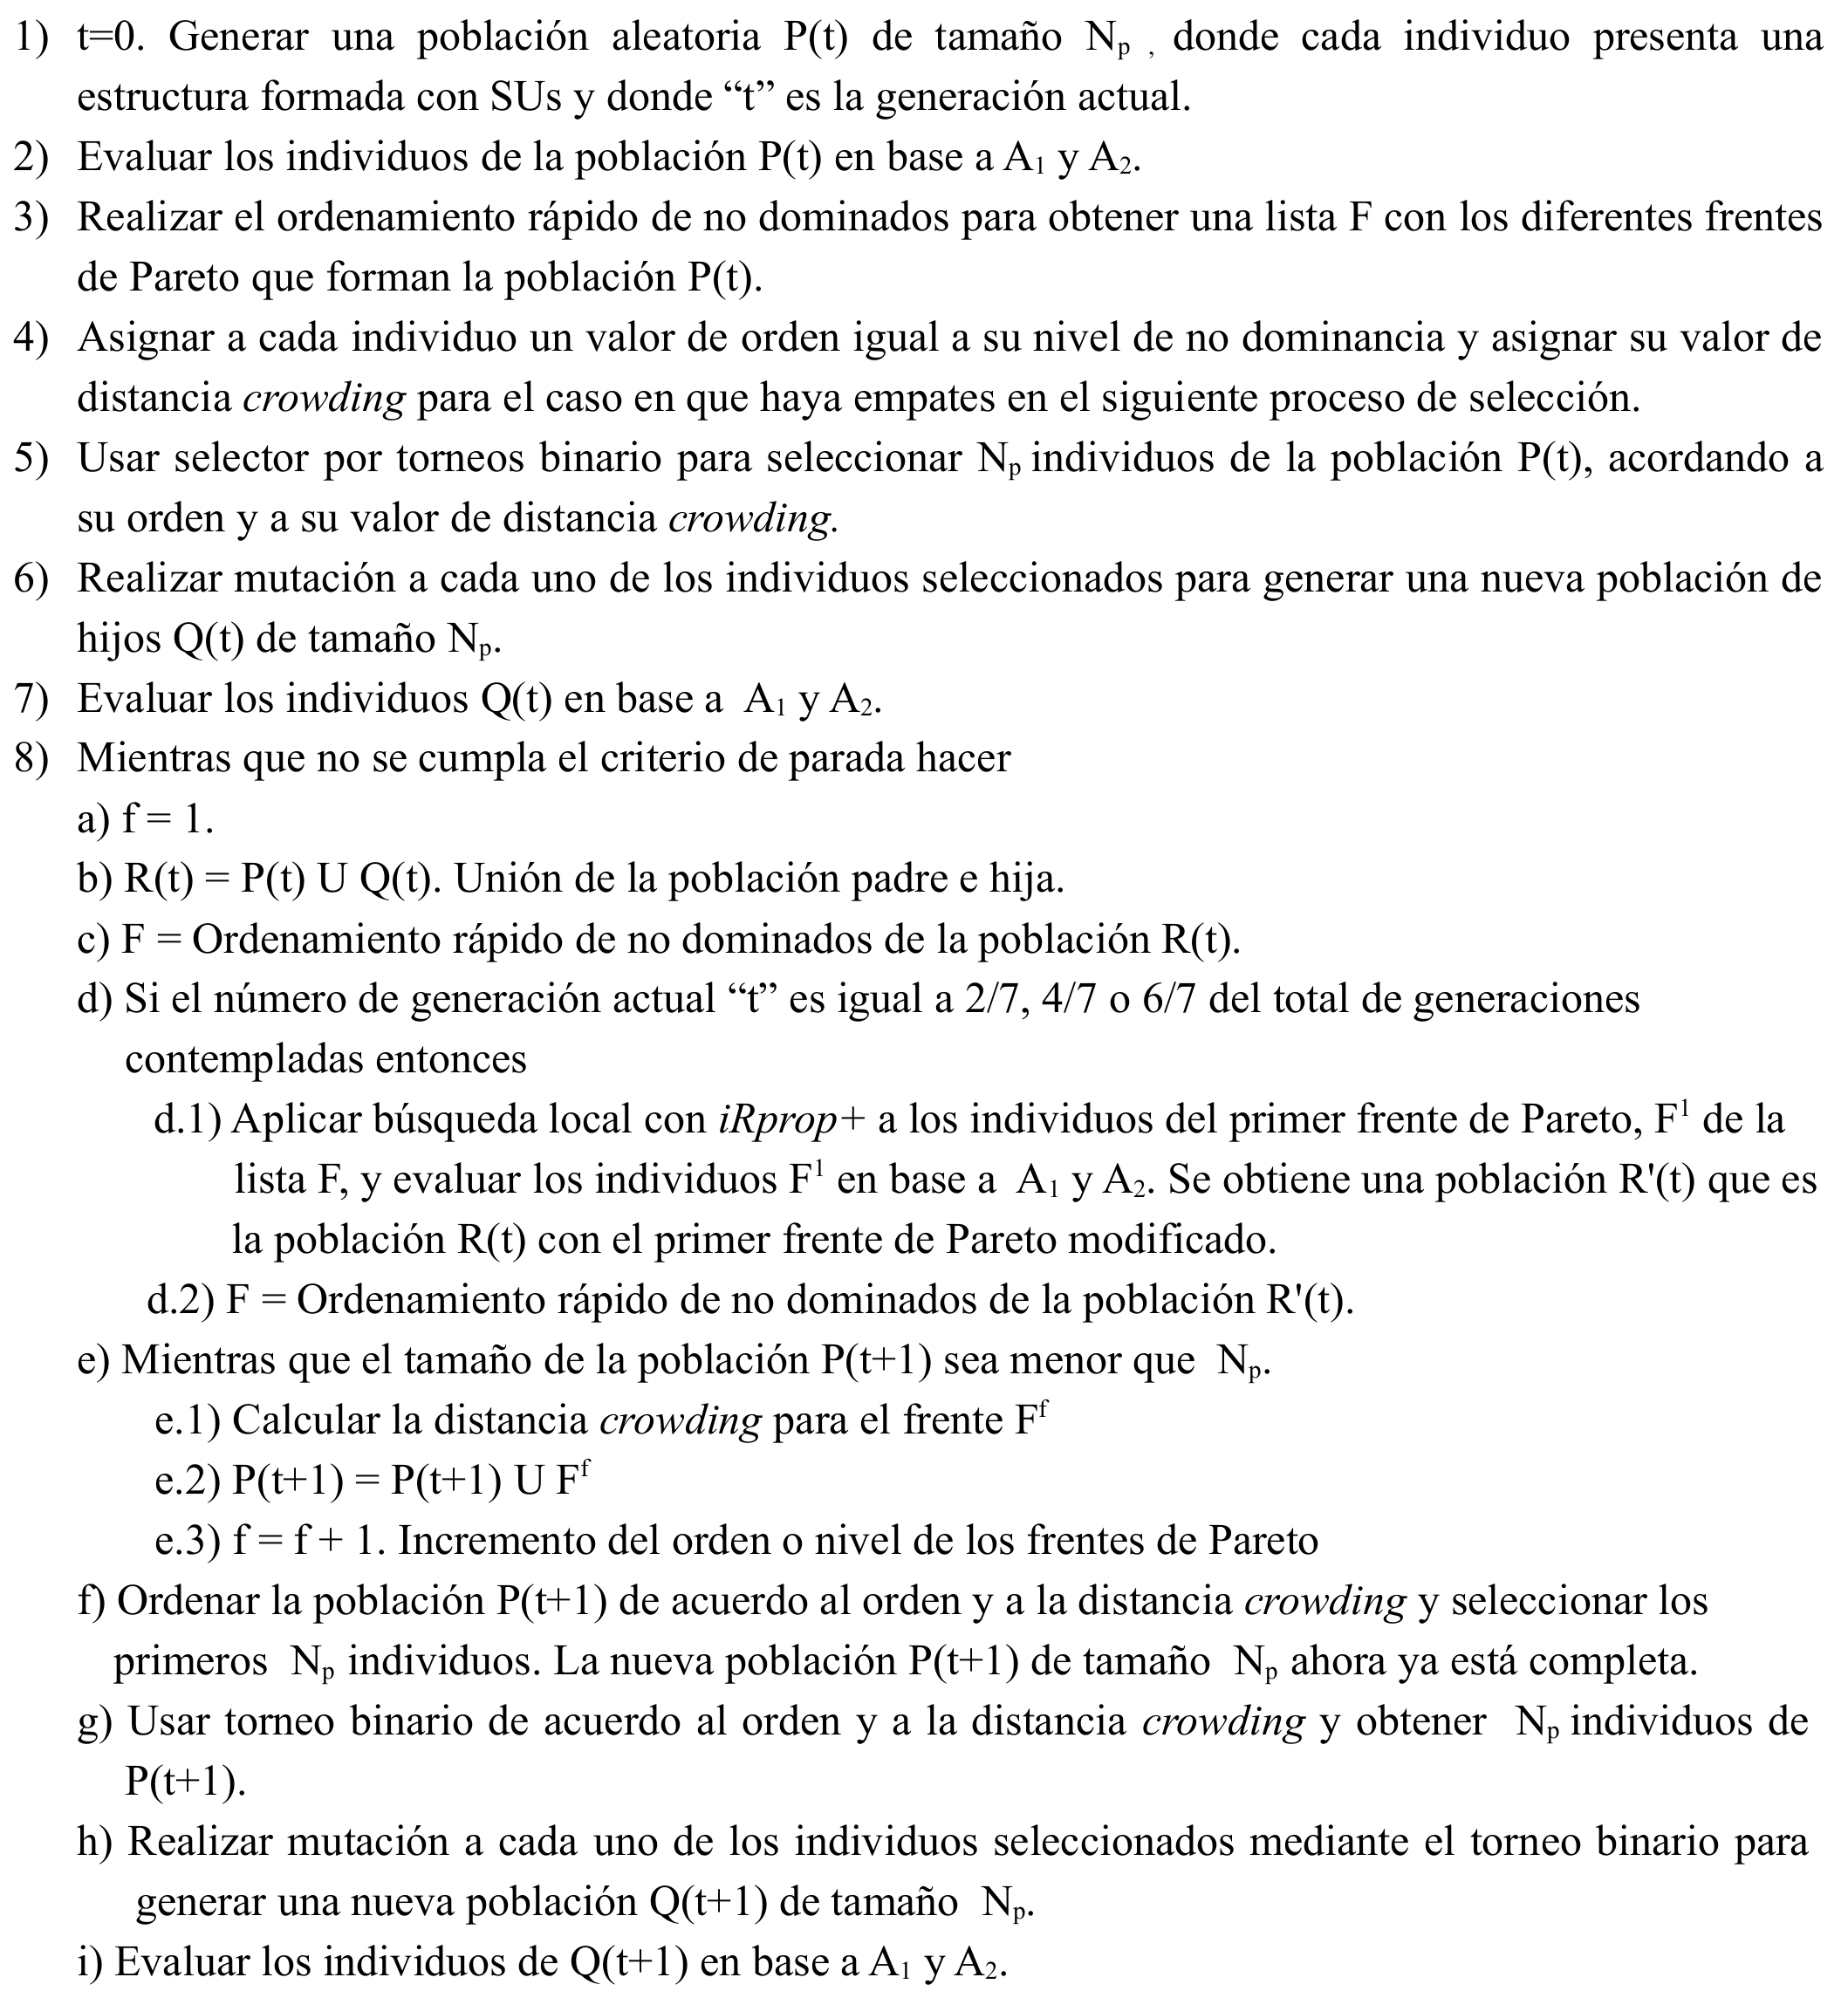
\includegraphics[keepaspectratio,width=12.5cm]{figuras/marcoMPENSGAII.jpg}
}
\caption{Pseudocódigo del marco general de MPENSGAII.}
\label{marcoMPENSGAII}
\end{figure}

\newpage

 \begin{figure}[!htp]
\centering
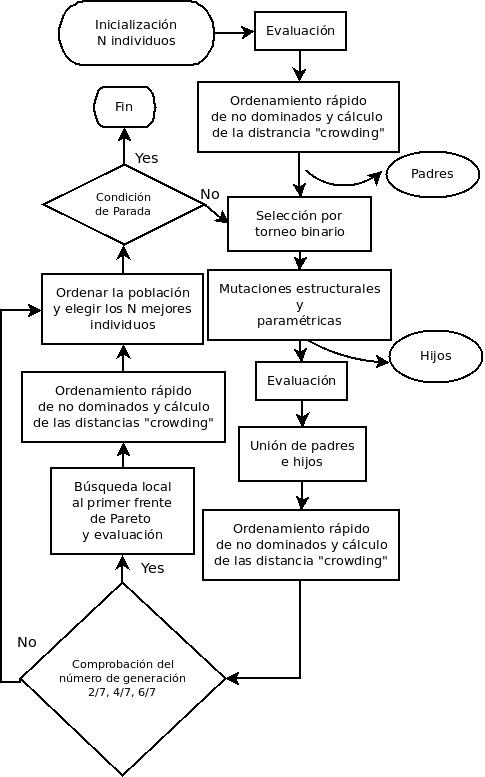
\includegraphics[keepaspectratio,width=8cm]{figuras/etapasMPENSGAII.jpg}
\caption{Etapas del algoritmo MPENSGAII.}
\label{etapasMPENSGAII}
\end{figure}

MPENSGAII comienza con la generación aleatoria de 100 ANNs con unidades de base de tipo
SU, es decir, el valor
de $N_{p}$ del paso 1 de la figura \ref{marcoMPENSGAII} es $N_{p}=100$. El valor de los
pesos asociados a los enlaces es un número aleatorio perteneciente al intervalo $\left[
-5,5\right] $ para los pesos de capa entrada-capa oculta y al intervalo $\left[
-10,10\right] $ para los pesos de capa
oculta-capa de salida. El número de neuronas en capa oculta se obtiene de la misma forma
que en el algoritmo CBFEP de capítulo anterior, es decir, considerando los parámetros
$m$, $M_{E}$ y $M_{I}$ (ver sección \ref{etapas} del capítulo \ref{evoMonoObjetivo}).

Una vez generada la población inicial, ésta se evalúa en base a
$A_{1}$ y $A_{2}$ (paso 2). Como tercer paso se hace el ordenamiento rápido de no
dominados, obteniendo una lista de frentes de Pareto. Una vez hecho esto, a cada individuo
se le asigna un valor de orden dependiendo del valor de no dominancia obtenido
en el paso anterior (1 para los individuos del primer frente, 2 para los del segundo,
...). También se asigna el valor de la distancia \textit{crowding}. Para ver con más
detalle como se realizan este tipo de operaciones consultar el algoritmo NSGAII
en \cite{Deb2002}.

Se pasa entonces a la etapa de selección de individuos. Ésta se realiza mediante un
torneo binario, de manera que se seleccionan $N_{p}$ individuos (paso 5). A los
individuos seleccionados se les aplica un operador de mutación y se etiquetan como una
nueva población (paso 6), aparte de la población inicial. Esta nueva población se evalúa
de la misma manera que en el paso 2. Una vez se tienen las dos poblaciones, comienza el
proceso evolutivo.

Primero se unen la población padre o inicial y la hija creada en los pasos anteriores,
formándose una población $R(t)$ (paso 8-b). A $R(t)$ se le aplica un ordenamiento rápido
de no dominados (paso 8-c) obteniendo una nueva lista de frentes. En este momento, si la
generación actual $t$ es igual a 2/7, 4/7 o 6/7 del total de generaciones del proceso
evolutivo, se pasa al proceso de LS. Concretamente se aplica iRprop+ al primer
frente de Pareto de la población  $R(t)$, y se evalúan los individuos. Se tiene por tanto
una población $R'(t)$  con los individuos del primer frente modificados. A $R'(t)$ se le
aplica de nuevo un ordenamiento rápido de no dominados.

Se haya utilizado o no la LS, a continuación se irá creando una
población $P(t+1)$ para la siguiente generación, de manera que ésta se genera
añadiendo individuos de la lista de frentes obtenida (paso 8-d.2) y en base a las
distancias \textit{crowding} de los individuos, hasta que el tamaño de $P(t+1)$ sea igual
o mayor a $N_{p}$ (paso e).

Cuando la población $P(t+1)$ está completa se ordena en base al orden de frente y a la
distancia \textit{crowding} y se seleccionan los primeros $N_{p}$ individuos. Entonces, la nueva
población $P(t+1)$ queda completa (paso f).

Pasamos de nuevo a realizar un proceso de selección por torneo binario, obteniendo  $N_{p}$
individuos de $P(t+1)$ (paso g).

A los individuos seleccionados se les aplica un operador de mutación, de manera que la
población $P(t+1)$ pasa a llamarse $Q(t+1)$ (paso h).

La población $Q(t+1)$ es evaluada, quedando preparada para iniciar la siguiente
generación del proceso evolutivo (paso i), el cual termina cuando se haya alcanzado el
número de generaciones indicadas al inicio del algoritmo, y que depende de cada base de
datos o problema.

\subsection{Diseño experimental} \label{disenio}
\noindent Para analizar el rendimiento de MPENSGAII hemos utilizado 17
conjuntos de datos del repositorio de la UCI \cite{UCI2007}, más otro interesante
conjunto que no pertenece a dicho repositorio, que se denomina BTX.

BTX (ver \cite{Hervas2008}) es un problema de clasificación que
consiste en discriminar entre diferentes tipos de
aguas contaminadas. El conjunto de datos  incluye un conjunto de 63 ejemplos de diferentes
aguas con
una determinada cantidad de Benceno, Tolueno y Xyleno, en concentraciones que se encuentran
entre los 5 y los 30 $\mu g/l$. Hay siete tipos de aguas contaminadas con el mismo número
de patrones por clase.

En la tabla \ref{tabla1MPENSGAII} se muestran las características de cada
conjunto de datos. La tabla está dividida en problemas binarios y problemas multi-clase.
Estos últimos, en general, son más difíciles de clasificar, ya que al aumentar
el número de clases, el valor de $p^*$ es más pequeño, y el rango de valores de $MS$ será
más amplio para valores altos de $C$ (ver sección \ref{propiedades} y \ref{balanceados}
del
capítulo \ref{medidasRendimiento}). La tabla muestra el número total de patrones por cada
conjunto de datos, el número de patrones en el conjunto de entrenamiento y en el
conjunto de generalización, el número de
variables de entrada, el número de clases, el número total de patrones por clase y el
valor de $p^*$.

El diseño experimental consiste en una partición estratificada del conjunto de datos con $3n/4$
patrones para
el conjunto de entrenamiento y $n/4$ patrones para el conjunto de generalización, siendo $n$ el
tamaño del conjunto.

%(PREGUNTAR COMO CENTRAR EL ENCABEZADO DE LA PENULTIMA COLUMNA)
\begin{table}[htb!]
\scriptsize
\caption{Características de los conjuntos de datos de la UCI y del conjunto BTX.}
\label{tabla1MPENSGAII}
\centering
\tabcolsep 1pt
\begin{tabular}{c c c c c c p{2.5cm} c}
\hline
\rowcolor[rgb]{0.70,0.85,1}\textbf{\textit{Conjunto}} & \textbf{Patrones} &
\textbf{Patrones} & \textbf{Patrones} &
\textbf{Variables} & \textbf{Clases} &
\textbf{Patrones} & $\mathbf{p^{*}}$ \\
\rowcolor[rgb]{0.70,0.85,1} & & \textbf{entrena.} & \textbf{generaliz.} & \textbf{de
entrada} & & \textbf{por clase} & \\ \hline
\multicolumn{8}{>{\columncolor[rgb]{0.70,0.85,1}}c}{Dos clases} \\ \hline
\rowcolor[rgb]{0.86,0.94,1}AustralianC & 690 & 517 & 173 & 51 & 2 & 307-383 & 0.4411 \\
\rowcolor[rgb]{0.86,0.94,1}BreastC & 286 & 215 & 71 & 15 & 2 & 201-85 & 0.2957 \\
\rowcolor[rgb]{0.86,0.94,1}BreastC-W & 699 & 524 & 175 & 9 & 2 & 458-241 & 0.3428 \\
\rowcolor[rgb]{0.86,0.94,1}German & 1000 & 750 & 250 & 61 & 2 & 700-300 & 0.3000 \\
\rowcolor[rgb]{0.86,0.94,1}HeartStatlog & 270 & 202 & 68 & 13 & 2 & 150-120 & 0.4411 \\
\rowcolor[rgb]{0.86,0.94,1}Ionosphere & 351 & 263 & 88 & 34 & 2 & 126-225 & 0.3636 \\
\rowcolor[rgb]{0.86,0.94,1}Pima & 768 & 576 & 192 & 8 & 2 & 500-268 & 0.3489 \\
\rowcolor[rgb]{0.86,0.94,1}Vote & 435 & 326 & 109 & 16 & 2 & 267-168 & 0.3853 \\ \hline
\multicolumn{8}{>{\columncolor[rgb]{0.70,0.85,1}}c}{Multiclase} \\ \hline
\rowcolor[rgb]{0.86,0.94,1}Autos & 205 & 152 & 53 & 72 & 6 & 67-3-22-54-32-27 & 0.0188 \\
\rowcolor[rgb]{0.86,0.94,1}Balance & 625 & 469 & 156 & 4 & 3 & 288-49-288 & 0.0641 \\
\rowcolor[rgb]{0.86,0.94,1}BTX & 63 & 42 & 21 & 3 & 7 & 9-9-9-9-9-9-9 & 0.1428 \\
\rowcolor[rgb]{0.86,0.94,1}Gene & 3175 & 2381 & 794 & 120 & 3 & 762-765-1648 & 0.2405 \\
\rowcolor[rgb]{0.86,0.94,1}Iris & 150 & 111 & 39 & 4 & 3 & 50-50-50 & 0.3333 \\
\rowcolor[rgb]{0.86,0.94,1}Lymphography & 148 & 111 & 37 & 38 & 4 & 2-81-61-4 & 0.0270 \\
\rowcolor[rgb]{0.86,0.94,1}Newthyroid & 215 & 161 & 54 & 5 & 3 & 150-35-30 & 0.1296 \\
\rowcolor[rgb]{0.86,0.94,1}Post-operatory & 90 & 67 & 23 & 20 & 3 & 2-24-64 & 0.0434 \\
\rowcolor[rgb]{0.86,0.94,1}Vowel & 990 & 737 & 253 & 10 & 11 & 90-90-90-90-90-\newline
90-90-90-90-90-90 & 0.0909 \\
\rowcolor[rgb]{0.86,0.94,1}Yeast & 1484 & 1112 & 372 & 8 & 10 & 30-20-429-244-163-\newline
51-44-35-5-463 & 0.0026 \\ \hline
\end{tabular}
\end{table}

Una vez que el frente de Pareto es construido, utilizamos dos estrategias de selección
automática de individuos, el mejor modelo en $E$ y el mejor modelo en $MS$, (extremos del frente de
Pareto). En la figura
\ref{obtencionResultados} se muestra la
metodología llevada a cabo a la hora de obtener resultados, la cual se detalla a
continuación:

En cada ejecución del algoritmo, una vez que se tiene el frente de Pareto de la
última generación del proceso evolutivo, se escogen los extremos del frente en
entrenamiento. Esto es, el mejor individuo en $E$, y el mejor individuo en
$MS$. A estos individuos los denominaremos individuo $EI$, para el
primer caso, e individuo $MSI$, para el segundo.

\begin{figure}[htb!]
\centering
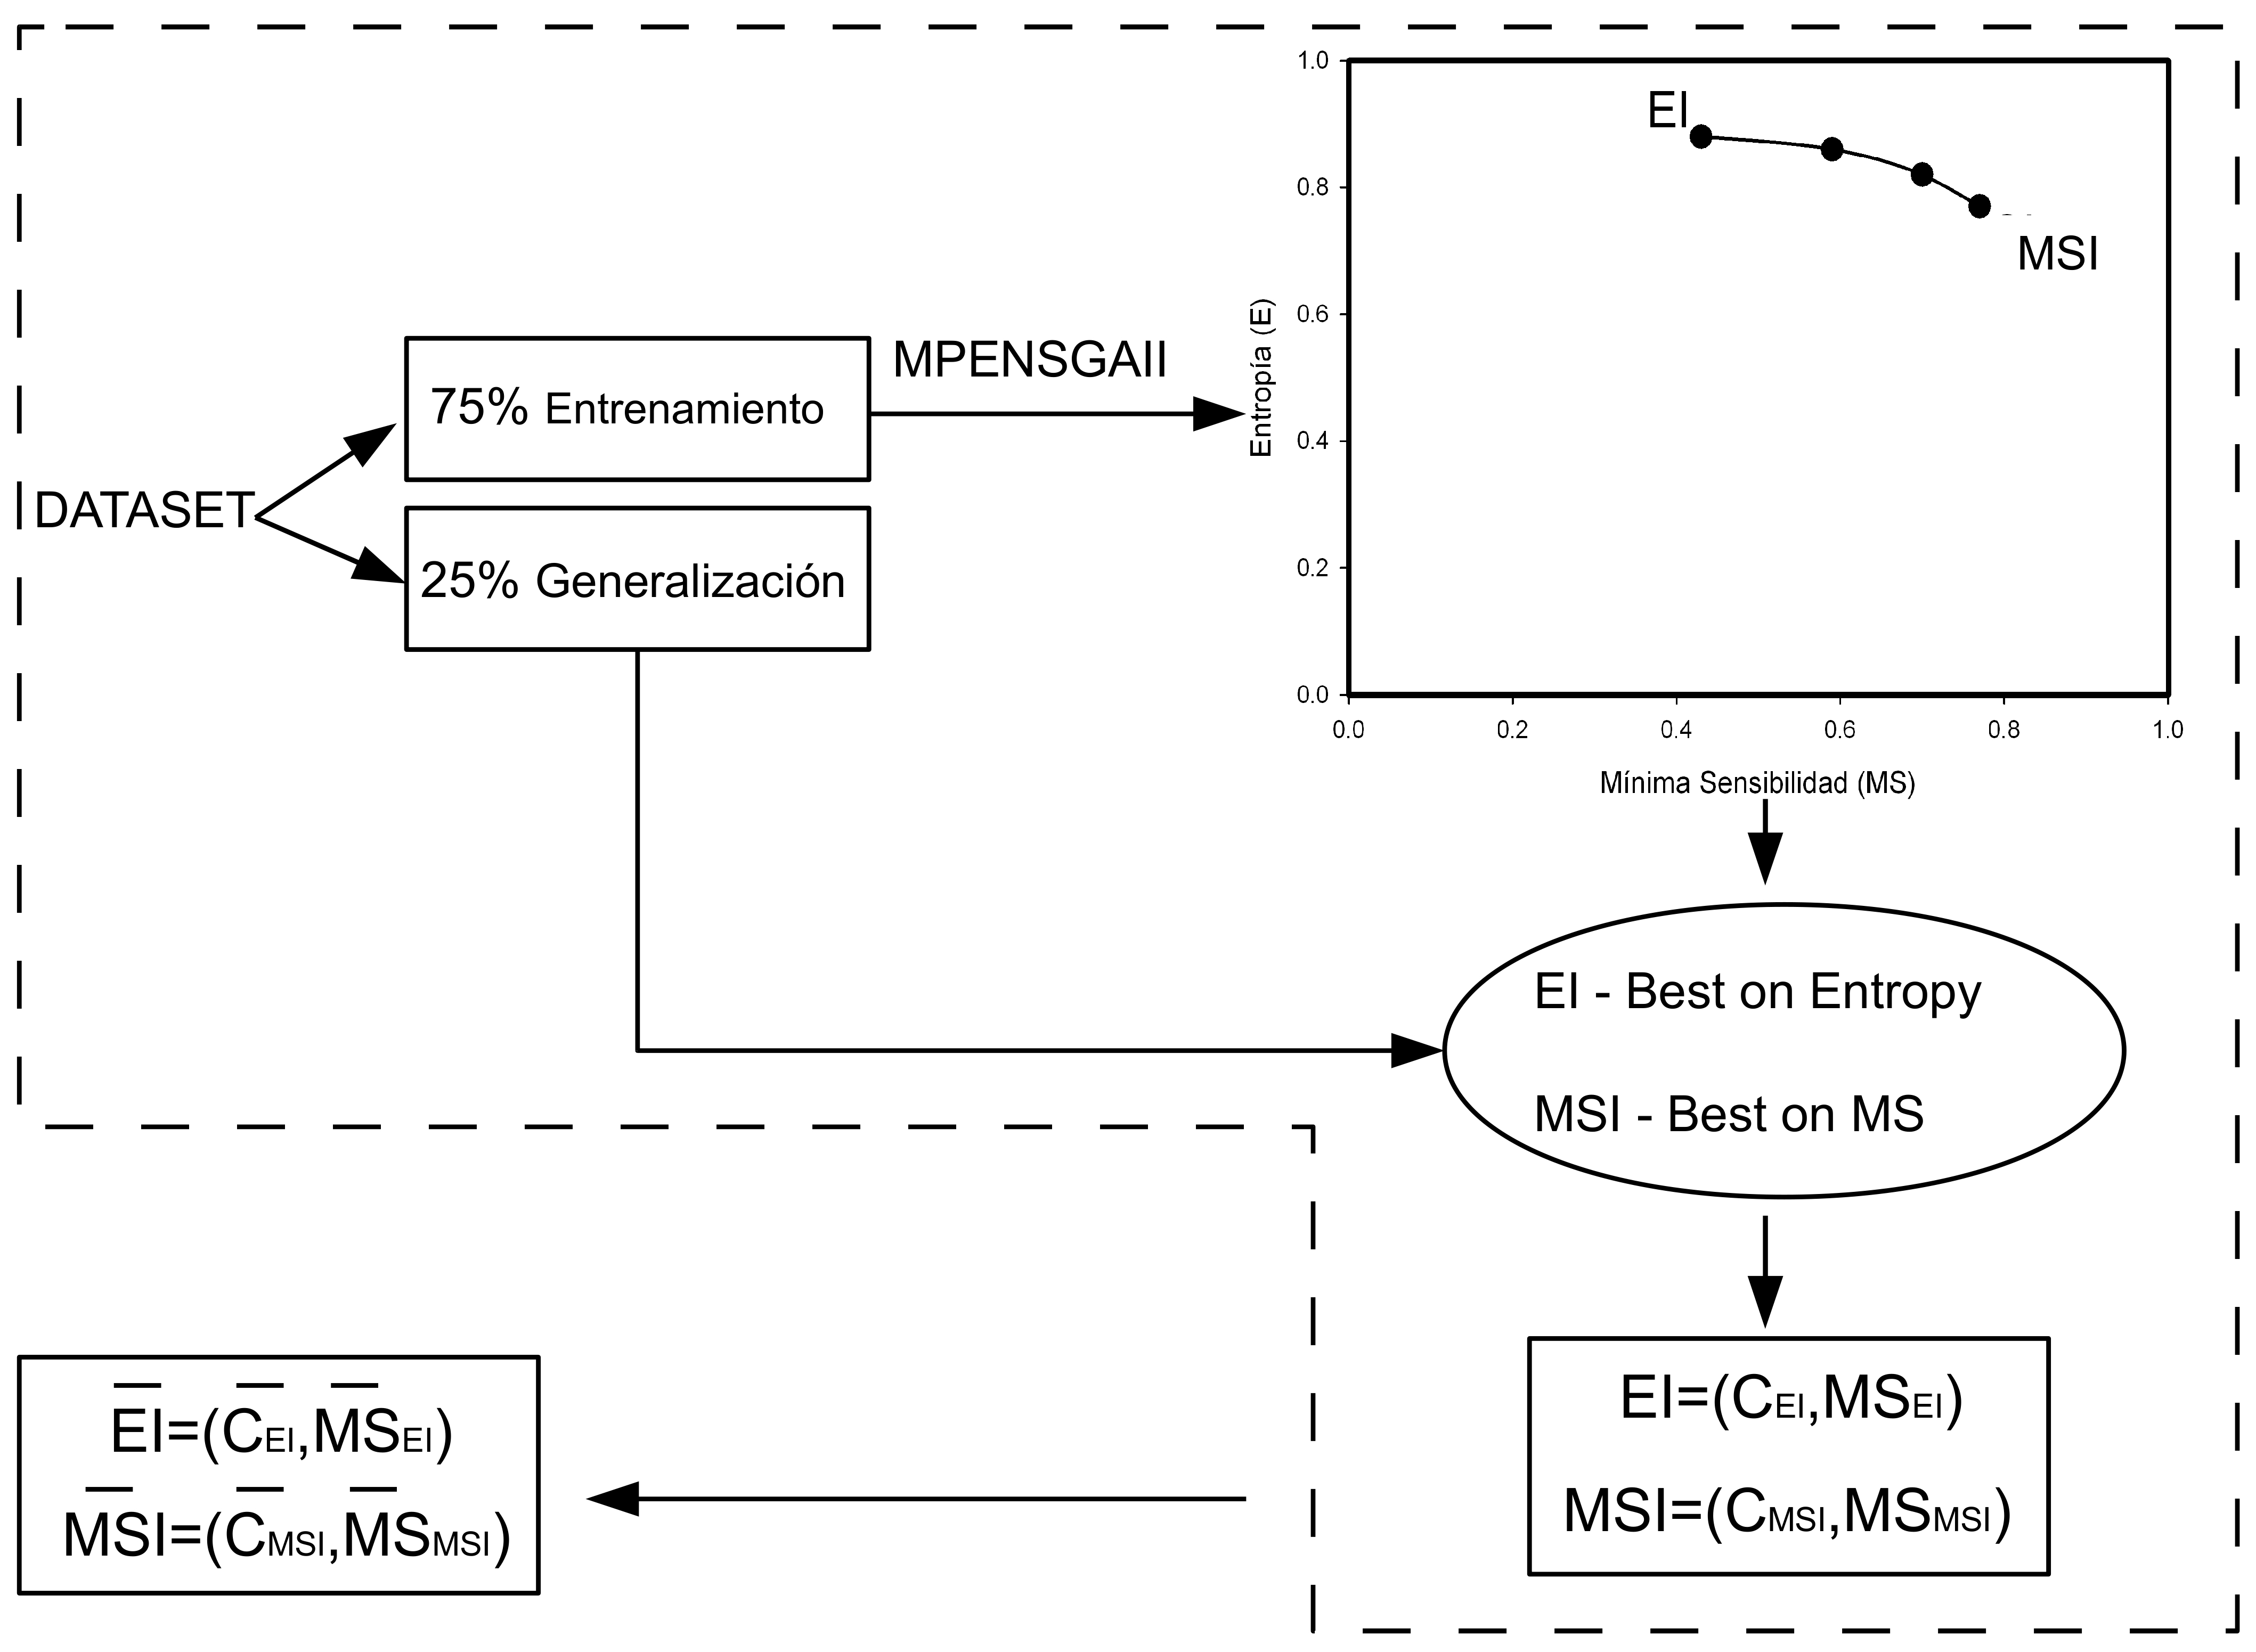
\includegraphics[keepaspectratio,width=13cm]{figuras/obtencionResultados.jpg}
\caption{Obtención de modelos a partir de MPENSGAII.}
\label{obtencionResultados}
\end{figure}

Una vez que tenemos los individuos del paso anterior se calcula su valor de precisión,
$C$, y de mínima sensibilidad, $MS$, sobre el conjunto de generalización. De esta manera,
tenemos para los extremos del frente dos pares de valores, $\displaystyle
EI=(C_{EI},MS_{EI})$ y
$\displaystyle MSI=(C_{MSI},MS_{MSI})$ de una ejecución de las 30 realizadas.

El proceso anterior se repite 30 veces obteniendo finalmente la media y la desviación
típica de los dos pares de valores para los individuos $EI$ y $MSI$, es decir,
$\displaystyle \overline{EI}=(\overline{C}_{EI},\overline{MS}_{EI})$ y
$\displaystyle \overline{MSI}=(\overline{C}_{MSI},\overline{MS}_{MSI})$, de forma que la
primera expresión muestra el rendimiento medio obtenido teniendo en cuenta solo los
mejores individuos en $E$, mientras que la segunda expresión muestra el rendimiento
medio teniendo en cuenta solo los mejores individuos en $MS$. Al
procedimiento de obtención automática del rendimiento medio teniendo en cuenta los
mejores individuos en $E$ (parte superior del frente) lo hemos llamado MPENSGAIIE, y al
procedimiento de obtención automática del rendimiento medio teniendo en cuenta los mejores
individuos en $MS$ (parte inferior del frente) lo hemos llamado MPENSGAIIS.

Todos los parámetros de MPENSGAII son comunes a los 18 experimentos, excepto $m$,
$M_{I}$, $M_{E}$ y el número de generaciones usadas, que al igual que para el
algoritmo  CBFEP depende del conjunto de datos. El valor de la población se ha
establecido en $N_{p}=100$. La probabilidad de mutación para cada operador es igual a
$1/5$. Para la mutación paramétrica hemos establecido valores de $r=0.95$ y de
temperatura inicial $T_{0}=1$. Para iRprop+, los parámetros adoptados son $\eta^{-}=0.5$
(tamaño de paso para el factor de decremento), $\eta^{+}=1.2$ (tamaño de paso para el
factor de incremento), $\bigtriangleup_{0} =0.0125$ (valor inicial de tamaño de paso para
los pesos, $\bigtriangleup_{ij}$),  $\bigtriangleup_{min} =0$ (tamaño mínimo de paso para
los pesos), $\bigtriangleup_{max} =50$ (tamaño máximo de paso para los pesos), $Epochs=25$
(número de épocas para la optimización local).

\subsection{Resultados} \label{resultadosMPENSGAII}
\noindent Hemos comparado MPENSGAII con dos algoritmos muy utilizados en el
entrenamiento de ANNs:
\begin{description}
\item[MPANN:] MPANN (\textit{Memetic Pareto Artificial Neural Networks})
\cite{Abbass2003} es un MOEA basado en DE \cite{Price2005} para el diseño de ANNs, que
optimiza dos objetivos: minimizar el $MSE$ y minimizar la complejidad de la red, teniendo
en cuenta el número de neuronas en capa oculta. MPANN utiliza el algoritmo BP como
procedimiento de LS.

Nosotros hemos implementado una versión de MPANN en Java utilizando el pseudocódigo
descrito en \cite{Abbass2003}, ya que no hay una versión de este algoritmo de libre
disposición. Para el algoritmo de LS hemos utilizado iRprop+ en vez de BP,
mejorando el procedimiento con respecto a BP \cite{Igel2000}. También hemos añadido a
la implementación la obtención de la $MS$ de todas las clases. MPANN utiliza la misma
estrategia automática de obtención de resultados
utilizada con MPENSGAII, es decir, se seleccionan los extremos del frente de Pareto
teniendo en cuenta a los mejores individuos en $MSE$ y a los mejores individuos en complejidad
(neuronas ocultas). Así, a las dos metodologías automáticas de obtención de resultados se
le ha llamado MPANN-MSE y MPANN-HN.

\item[TRAINDIFFEVOL:] TRAINDIFFEVOL (\textit{Differential Evolution Training Algorithm for
Feed-Forward Neural Networks}) \cite{Jarno2003} es un algoritmo mono-objetivo para
entrenar perceptrones multicapa mediante el error cuadrático medio de los
pesos regularizado (\textit{Mean Square Error Regularized}, MSEREG) y está basado en DE
\cite{Price2005}.

Para poder realizar adecuadamente una comparación con los resultados obtenidos con este
método hemos modificado el código fuente de TRAINDIFFEVOL, de forma que se pueda obtener
la sensibilidad para cada una de las clases de un problema y así poder calcular
$MS$. TRAINDIFFEVOL está disponible en la web en código Matlab
\footnote{http://www.it.lut.fi/project/nngenetic}.
\end{description}

Las tablas \ref{tabla2MPENSGAII} y \ref{tabla2MPENSGAII-b} presentan los valores de las medias y
desviaciones típicas
para $C$ y $MS$ en generalización para los mejores modelos en cada ejecución y para cada
conjunto de datos.

\begin{landscape}
\tabcolsep 2.5pt
\scriptsize
\begin{longtable}{cccccccc}
\caption{Resultados estadísticos para MPENSGAIIE, MPENSGAIIS, TRAINDIFFEVOL, MPANN-MSE y
MPANN-HN en generalización para los conjuntos de datos binarios.}
\label{tabla2MPENSGAII} \\
\hline
\rowcolor[rgb]{0.70,0.85,1}\textbf{Conjunto} & \textbf{Algoritmo} & $\mathbf{C(\%)}$ &
$\mathbf{MS(\%)}$ & \textbf{Conjunto} & \textbf{Algoritmo} & $\mathbf{C(\%)}$ &
$\mathbf{MS(\%)}$ \\ \hline
\multicolumn{8}{>{\columncolor[rgb]{0.70,0.85,1}}c}{\textbf{Dos clases}} \\ \hline
\endfirsthead
\hline
% \rowcolor[rgb]{0.70,0.85,1}\textbf{Conjunto} & \textbf{Algoritmo} & $\mathbf{C(\%)}$ &
% $\mathbf{MS(\%)}$ & \textbf{Conjunto} & \textbf{Algoritmo} & $\mathbf{C(\%)}$ &
% $\mathbf{MS(\%)}$ \\
% \hline \multicolumn{8}{r}{{Continúa en la siguiente página}} \\ \hline
% \endfoot
% \hline \hline
% \endlastfoot
\rowcolor[rgb]{0.86,0.94,1}Australian Card & MPENSGA2E & \textit{88.07$\pm$1.57} &
\textit{86.13$\pm$2.73} & Breast Cancer & MPENSGA2E & \textbf{69.34$\pm$2.30} &
\textit{28.89$\pm$9.10} \\
\rowcolor[rgb]{0.86,0.94,1}& MPENSGA2S & \textbf{88.25$\pm$1.39} & \textbf{86.84$\pm$2.00}
&  & MPENSGA2S & 63.99$\pm$3.11 & \textbf{53.09$\pm$6.58} \\
\rowcolor[rgb]{0.86,0.94,1}& TRAINDIFFEVOL & 81.93$\pm$7.78 & 72.90$\pm$18.04\textbf{} &
& TRAINDIFFEVOL & \textit{68.94$\pm$2.82} & 26.35$\pm$11.17 \\
\rowcolor[rgb]{0.86,0.94,1}& MPANN-MSE & 87.59$\pm$1.18\textbf{} & 85.95$\pm$1.98\textbf{}
&  & MPANN-MSE & 66.53$\pm$3.07 & 28.73$\pm$14.23\textbf{} \\
\rowcolor[rgb]{0.86,0.94,1}& MPANN-HN & 87.78$\pm$2.49\textbf{} & 85.83$\pm$4.43\textbf{}
&  & MPANN-HN & 66.53$\pm$3.07 & 28.41$\pm$14.34\textbf{} \\ \hline
\rowcolor[rgb]{0.86,0.94,1}Breast Cancer Wisconsin & MPENSGA2E & 95.87$\pm$0.61 &
90.94$\pm$1.68 & German & MPENSGA2E & \textbf{75.31$\pm$1.44} & \textit{51.16$\pm$4.10} \\
\rowcolor[rgb]{0.86,0.94,1}& MPENSGA2S & 95.60$\pm$0.85 & 90.72$\pm$1.84\textbf{} &  &
MPENSGA2S & 71.55$\pm$1.87 & \textbf{68.80$\pm$3.11} \\
\rowcolor[rgb]{0.86,0.94,1}& TRAINDIFFEVOL & 93.98$\pm$1.75 & 86.22$\pm$4.69\textbf{} &  &
TRAINDIFFEVOL & 71.73$\pm$2.11 & 28.36$\pm$19.90 \\
\rowcolor[rgb]{0.86,0.94,1}& MPANN-MSE & \textit{96.04$\pm$1.08} & \textit{92.75$\pm$3.40}
&  & MPANNMSE & 73.61$\pm$1.80 & 48.89$\pm$5.33\textbf{} \\
\rowcolor[rgb]{0.86,0.94,1}& MPANN-HN & \textbf{96.27$\pm$1.00} & \textbf{93.30$\pm$3.36}
&  & MPANN-HN & \textit{73.76$\pm$1.77} & 48.76$\pm$5.44\textbf{} \\ \hline
\rowcolor[rgb]{0.86,0.94,1}Heart Statlog & MPENSGA2E & \textbf{78.28$\pm$1.76} &
61.89$\pm$2.09 & Ionosphere & MPENSGA2E & \textbf{92.65$\pm$2.22} &
\textbf{82.71$\pm$5.36} \\
\rowcolor[rgb]{0.86,0.94,1}& MPENSGA2S & \textit{77.50$\pm$1.73} & \textit{62.67$\pm$2.38}
&  & MPENSGA2S & \textit{92.08$\pm$2.30} & \textit{82.40$\pm$4.14} \\
\rowcolor[rgb]{0.86,0.94,1}& TRAINDIFFEVOL & 76.32$\pm$2.02 & 60.00$\pm$3.82 &  &
TRAINDIFFEVOL & 85.23$\pm$4.68 & 65.31$\pm$9.11 \\
\rowcolor[rgb]{0.86,0.94,1}& MPANN-MSE & 76.91$\pm$1.10 & \textbf{62.68$\pm$2.21} &  &
MPANN-MSE & 91.10$\pm$2.37 & 79.17$\pm$5.99 \\
\rowcolor[rgb]{0.86,0.94,1}& MPANN-HN & 76.91$\pm$1.10 & \textbf{62.68$\pm$2.21} &  &
MPANN-HN & 91.10$\pm$2.37 & 79.17$\pm$5.99 \\ \hline
\rowcolor[rgb]{0.86,0.94,1}Pima & MPENSGA2E & \textbf{78.99$\pm$1.81} &
\textit{60.45$\pm$2.59} & Vote & MPENSGA2E & \textbf{94.74$\pm$0.87} &
\textbf{93.42$\pm$1.70} \\
\rowcolor[rgb]{0.86,0.94,1}& MPENSGA2S & 76.96$\pm$2.09\textbf{} & \textbf{72.69$\pm$3.07}
&  & MPENSGA2S & \textit{94.68$\pm$0.91} & \textit{93.38$\pm$1.61}\textbf{\textit{}} \\
\rowcolor[rgb]{0.86,0.94,1}& TRAINDIFFEVOL & 70.59$\pm$3.50 & 37.29$\pm$19.74 &  &
TRAINDIFFEVOL & 93.39$\pm$1.69 & 91.99$\pm$1.69 \\
\rowcolor[rgb]{0.86,0.94,1}& MPANN-MSE & \textit{78.54$\pm$1.80} & 59.65$\pm$3.71 &  &
MPANN-MSE & 94.19$\pm$1.28 & 92.53$\pm$2.34 \\
\rowcolor[rgb]{0.86,0.94,1}& MPANN-HN & 78.28$\pm$2.03 & 58.86$\pm$3.86 &  & MPANN-HN &
94.19$\pm$1.28 & 92.53$\pm$2.34 \\ \hline
\multicolumn{8}{l}{Los mejores resultados están en \textbf{negrita} y los segundos mejores
resultados se encuentran en \textit{itálica}.} \\
\end{longtable}
\end{landscape}

\begin{landscape}
\tabcolsep 2.5pt
\scriptsize
\begin{longtable}{cccccccc}
\caption{Resultados estadísticos para MPENSGAIIE, MPENSGAIIS, TRAINDIFFEVOL, MPANN-MSE y
MPANN-HN en generalización para los conjuntos de datos multiclase.}
\label{tabla2MPENSGAII-b} \\
\hline
\rowcolor[rgb]{0.70,0.85,1}\textbf{Conjunto} & \textbf{Algoritmo} & $\mathbf{C(\%)}$ &
$\mathbf{MS(\%)}$ & \textbf{Conjunto} & \textbf{Algoritmo} & $\mathbf{C(\%)}$ &
$\mathbf{MS(\%)}$ \\ \hline
\multicolumn{8}{>{\columncolor[rgb]{0.70,0.85,1}}c}{\textbf{Multi-clase}} \\ \hline
\endfirsthead
\hline
% \rowcolor[rgb]{0.70,0.85,1}\textbf{Conjunto} & \textbf{Algoritmo} & $\mathbf{C(\%)}$ &
% $\mathbf{MS(\%)}$ & \textbf{Conjunto} & \textbf{Algoritmo} & $\mathbf{C(\%)}$ &
% $\mathbf{MS(\%)}$ \\
% \hline
% \multicolumn{8}{>{\columncolor[rgb]{0.70,0.85,1}}c}{\textbf{Multi-clase}} \\ \hline
% \endhead
% \multicolumn{8}{>{\columncolor[rgb]{0.70,0.85,1}}c}{\textbf{Multi-clase}} \\ \hline
\rowcolor[rgb]{0.86,0.94,1}Autos & MPENSGA2E & \textbf{66.67$\pm$4.06} &
\textit{39.64$\pm$14.91} & Balance & MPENSGA2E & \textbf{94.02$\pm$1.53} & 42.66$\pm$17.00
\\
\rowcolor[rgb]{0.86,0.94,1}& MPENSGA2S & \textit{66.04$\pm$4.78} &
\textbf{42.28$\pm$10.97} &  & MPENSGA2S & 92.48$\pm$2.16 & \textbf{83.74$\pm$8.19} \\
\rowcolor[rgb]{0.86,0.94,1}& TRAINDIFFEVOL & 26.79$\pm$7.49 & 0.00$\pm$0.00 &  &
TRAINDIFFEVOL & 87.12$\pm$2.56 & 2.00$\pm$6.10 \\
\rowcolor[rgb]{0.86,0.94,1}& MPANN-MSE & 48.42$\pm$3.71 & 0.00$\pm$0.00 &  & MPANN-MSE &
\textit{92.94$\pm$1.81} & \textit{60.00$\pm$14.14} \\
\rowcolor[rgb]{0.86,0.94,1} & MPANN-HN & 48.42$\pm$3.71 & 0.00$\pm$0.00 &  & MPANN-HN &
\textit{92.94$\pm$1.81} & \textit{60.00$\pm$14.14} \\ \hline
\rowcolor[rgb]{0.86,0.94,1}BTX & MPENSGA2E & \textbf{85.56$\pm$5.66} &
\textbf{61.11$\pm$12.63} & Gene & MPENSGA2E & \textit{86.42$\pm$2.04} &
\textit{80.85$\pm$3.45}\textbf{\textit{}} \\
\rowcolor[rgb]{0.86,0.94,1} & MPENSGA2S & \textit{85.40$\pm$5.99} &
\textit{60.00$\pm$13.56} &  & MPENSGA2S & \textbf{86.47$\pm$2.28} &
\textbf{81.77$\pm$2.77} \\
\rowcolor[rgb]{0.86,0.94,1} & TRAINDIFFEVOL & 71.11$\pm$3.94 & 1.11$\pm$6.09 &  &
TRAINDIFFEVOL & 60.88$\pm$7.12 & 34.97$\pm$9.11 \\
\rowcolor[rgb]{0.86,0.94,1} & MPANN-MSE & 72.38$\pm$10.85 & 13.33$\pm$29.81 &  & MPANN-MSE
& 75.11$\pm$4.98 & 36.20$\pm$3.87 \\
\rowcolor[rgb]{0.86,0.94,1} & MPANN-HN & 69.52$\pm$11.46 & 13.33$\pm$29.81 &  & MPANN-HN &
75.11$\pm$4.98 & 36.20$\pm$3.87  \\ \hline
\rowcolor[rgb]{0.86,0.94,1}Iris & MPENSGA2E & \textbf{97.18$\pm$0.78} &
\textbf{91.54$\pm$2.35} & Lymphography & MPENSGA2E & \textbf{85.05$\pm$4.24} &
\textbf{5.17$\pm$19.67} \\
\rowcolor[rgb]{0.86,0.94,1} & MPENSGA2S & 96.50$\pm$1.43\textbf{} & 89.74$\pm$3.69 &  &
MPENSGA2S & \textbf{85.05$\pm$4.24} & \textbf{5.17$\pm$19.67} \\
\rowcolor[rgb]{0.86,0.94,1}& TRAINDIFFEVOL & \textit{97.18$\pm$1.03} &
\textit{91.54$\pm$3.10} &  & TRAINDIFFEVOL & \textit{81.98$\pm$4.62} & 0.00$\pm$0.00 \\
\rowcolor[rgb]{0.86,0.94,1}& MPANN-MSE & 95.29$\pm$9.85 & 86.15$\pm$29.51 &  & MPANN-MSE
& 80.45$\pm$5.96 & 0.00$\pm$0.00 \\
\rowcolor[rgb]{0.86,0.94,1} & MPANN-HN & 94.52$\pm$11.24 & 83.84$\pm$33.70 &  & MPANN-HN &
80.72$\pm$6.05 & 0.00$\pm$0.00 \\ \hline
\rowcolor[rgb]{0.86,0.94,1}Newthyroid & MPENSGA2E &
\textit{95.12$\pm$2.31}\textbf{\textit{}} & \textit{74.81$\pm$10.08} & Post-op & MPENSGA2E
& 67.83$\pm$3.89 & 0.00$\pm$0.00\textbf{} \\
\rowcolor[rgb]{0.86,0.94,1} & MPENSGA2S & \textbf{95.56$\pm$2.15} &
\textbf{75.08$\pm$10.67} &  & MPENSGA2S & 38.12$\pm$16.6 & \textbf{3.96$\pm$12.97} \\
\rowcolor[rgb]{0.86,0.94,1}& TRAINDIFFEVOL & 91.11$\pm$4.77 & 59.47$\pm$22.74 &  &
TRAINDIFFEVOL & \textbf{69.57$\pm$1.14} & 0.00$\pm$0.00 \\
\rowcolor[rgb]{0.86,0.94,1} & MPANN-MSE & 94.87$\pm$3.81 & 72.11$\pm$22.29 &  & MPANN-MSE
& \textit{68.84$\pm$2.81} & 0.00$\pm$0.00 \\
\rowcolor[rgb]{0.86,0.94,1} & MPANN-HN & 94.87$\pm$3.81 & 72.11$\pm$22.29 &  & MPANN-HN &
\textit{68.84$\pm$2.81} & 0.00$\pm$0.00 \\ \hline
\rowcolor[rgb]{0.86,0.94,1}Vowel & MPENSGA2E & \textbf{79.51$\pm$3.19} &
\textit{57.39$\pm$9.84} & Yeast & MPENSGA2E & \textbf{59.91$\pm$0.98} & 0.00$\pm$0.00 \\
\rowcolor[rgb]{0.86,0.94,1} & MPENSGA2S & \textit{77.36$\pm$3.90} &
\textbf{57.97$\pm$6.07} &  & MPENSGA2S & \textit{53.21$\pm$4.49} &
\textbf{12.13$\pm$12.20} \\
\rowcolor[rgb]{0.86,0.94,1} & TRAINDIFFEVOL & 40.83$\pm$2.80 & 0.00$\pm$0.00 &  &
TRAINDIFFEVOL & 37.61$\pm$5.16 & 0.00$\pm$0.00 \\
\rowcolor[rgb]{0.86,0.94,1} & MPANN-MSE & 41.66$\pm$4.21 & 0.00$\pm$0.00 &  & MPANN-MSE &
48.87$\pm$3.53 & 0.00$\pm$0.00 \\
\rowcolor[rgb]{0.86,0.94,1} & MPANN-HN & 41.66$\pm$4.21 & 0.00$\pm$0.00 &  & MPANN-HN &
48.87$\pm$3.53 & 0.00$\pm$0.00 \\ \hline
\multicolumn{8}{l}{Los mejores resultados están en \textbf{negrita} y los segundos mejores
resultados se encuentran en \textit{itálica}.} \\
\end{longtable}
\end{landscape}

En general, los mejores resultados se obtienen con MPENSGAIIE o MPENSGAIIS en todos los
conjuntos de datos, excepto para Breast Cancer Wisconsin, Heart-Statlog y Post-op. La tabla
\ref{tabla3MPENSGAII} resume los resultados, incluyendo la precisión
media en generalización, $\overline{C}_{G}(\%)$, y la $MS$ media,
$\overline{MS}_{G}(\%)$, para todos los conjuntos y métodos. Se muestra además el
orden de cada método en cada conjunto ($R=1$ para el método con mejor
rendimiento y $R=5$ para el peor), y el orden medio en $C$
($\overline{R}_{CG}$) y en $MS$ ($\overline{R}_{MSG}$). Si se
analizan estos resultados podemos realizar los siguientes comentarios:
\begin{enumerate}
	\item La metodología MPENSGAIIE obtiene el mejor resultado en $C$ en 13 de los 18
conjuntos, el segundo mejor resultado en otros tres, la mejor media en precisión
($\overline{C}_{G}=82.81\%$) y el mejor orden medio ($\overline{R}_{CG}$). En
$MS$, la metodología MPENSGAIIE obtiene el mejor resultado en 5 conjuntos y el segundo
mejor
resultado en otros 8. También obtiene el segundo mejor resultado medio en $MS$
($\overline{MS}_{G}=55.70\%$) y el segundo mejor orden medio en $MS$
($\overline{R}_{MSG}$). Teniendo en cuesta estos resultados, deberíamos utilizar esta
metodología (desde un punto de vista cuantitativo) si nuestro objetivo es obtener
clasificadores con buenos resultados en $C$ y resultados más que aceptables en $MS$.
\begin{table}[!htb]
\renewcommand{\arraystretch}{1.2}
\caption{Media en precisión ($\overline{C}_G(\%)$) y mínima sensibilidad
($\overline{MS}_G(\%)$) en generalización, orden medio en precisión
($\overline{R}_{CG}$) y orden medio en mínima sensibilidad
($\overline{R}_{MSG}$) en generalización para los diferentes métodos evaluados con los 18
conjuntos.}
\label{tabla3MPENSGAII}
\centering
\begin{tabular}{ccccc} \hline
\rowcolor[rgb]{0.70,0.85,1} &
\multicolumn{2}{>{\columncolor[rgb]{0.70,0.85,1}}c}{\textbf{Precisión}} &
\multicolumn{2}{>{\columncolor[rgb]{0.70,0.85,1}}c}{\textbf{Mínima Sensibilidad}} \\
\cline{2-5}
\rowcolor[rgb]{0.70,0.85,1}\textbf{Algoritmo} & $\mathbf{\overline{C}_{G}(\%)}$ &
$\mathbf{\overline{R}_{CG}}$ & \textbf{$\mathbf{\overline{MS}_{G}(\%)}$} &
$\mathbf{\overline{R}_{MSG}}$ \\ \hline
\rowcolor[rgb]{0.86,0.94,1}MPENSGA2E & \textbf{82.81} & \textbf{1.56} & \textit{55.70} &
\textit{2.17} \\
\rowcolor[rgb]{0.86,0.94,1}MPENSGA2S & \textit{79.82} & \textit{2.75} & \textbf{62.32} &
\textbf{1.56} \\
\rowcolor[rgb]{0.86,0.94,1}TRAINDIFFEVOL & 73.26 & 3.97 & 37.10 & 4.21 \\
\rowcolor[rgb]{0.86,0.94,1}MPANNMSE & 76.85 & 3.36 & 44.44 & 3.41 \\
\rowcolor[rgb]{0.86,0.94,1}MPANN-HN & 76.68 & 3.36 & 44.26 & 3.65 \\ \hline
\multicolumn{5}{l}{El mejor resultado se encuentra en \textbf{negrita} y el segundo mejor}\\
\multicolumn{5}{l}{resultado en \textit{itálica}.} \\
\end{tabular}
\end{table}
	\item Por otro lado, los resultados de MPENSGA2S muestran que, en $C$, es el mejor
	método para 4 conjuntos de datos, y el segundo mejor para otros 7, obteniendo el segundo mejor
resultado medio en precisión ($\overline{C}_{G}=79.82\%$) y el segundo mejor
orden medio en precisión ($\overline{R}_{CG}=2.75$). En $MS$, obtiene los
mejores resultados para 12 conjuntos de datos, el segundo mejor resultado para otros 4, la mejor
$MS$ media ($\overline{MS}_{G}=62.32\%$) y el mejor orden medio en
$MS$ ($\overline{R}_{MSG}=1.56$). Esta metodología se debería escoger si
nuestro objetivo es obtener clasificadores con buenos resultados en $MS$ y con valores
más que aceptables en $C$.
	\item Hemos observado una tendencia a clasificar la clase mayoritaria al analizar las
matrices de confusión mediante los modelos optimizados con el algoritmo TRAINDIFFEVOL.
Por esta razón TRAINDIFFEVOL obtiene mejores resultados cuando se aplica a problemas de
clasificación binaria o problemas bien balanceados, pero obtiene un peor rendimiento
cuando se aplica a problemas multi-clase o problemas muy desbalanceados.
	\item MPENSGA2E obtiene el mejor valor en $C$ y en $MS$ para
los conjuntos Ionosphere, Vote, BTX, Iris y Lymphography.
	\item MPENSGA2S obtiene el mejor valor valor en $C$ y $MS$ para Australian Card, Gene,
Lymphography y Newthyroid.
	\item Los conjuntos Autos, Lymphography, Post-op y Yeast necesitan de una mención
especial, ya que son problemas de difícil clasificación para todas las metodologías,
dado que están desbalanceados (observe en la tabla \ref{tabla2MPENSGAII} como estos
conjuntos tienen un valor de $p^*$ menor a $0.05$), haciendo que una mejora en
$MS$ sea difícil. A pesar de que el porcentaje de clasificación es aceptable, el valor de
$MS$ es muy bajo, debido a que la clase minoritaria tiene 3, 2, 2 y 5 patrones
respectivamente en cada uno de los conjuntos de datos mencionados. MPENSGA2S obtiene en $MS$: un
$42.28\%$ en media en Autos, un $5.17\%$
en Lymphography, un $3.96\%$ en Post-op y un $12.13\%$ en Yeast, sin reducir
dramáticamente la media en $C$ (ver tabla \ref{tabla2MPENSGAII}), mientras que el valor
de $MS$ con otras metodologías tienen una media de $0.00\%$. Cuando el problema está
muy desbalanceado, como en el caso de Autos y Lymphography, es muy difícil mejorar los
niveles de $MS$. Estos casos sugieren que en un futuro trabajo se integren técnicas de
remuestreo \cite{Chawla2002} en nuestra metodología.
\end{enumerate}

Para determinar si hay diferencias estadísticas significativas en los resultados
observados para cada método con los diferentes conjuntos de datos, se han realizado dos
test de Friedman no paramétricos \cite{Friedman1940} con el orden de $C_{G}$ y
$MS_{G}$ de los mejores modelos. El uso de test no paramétricos está justificado en este
caso, ya que un test previo de normalidad de Kolmogorov-Smirnof y de igualdad de
varianzas de Levene de los valores de $C_{G}$ y $MS_{G}$, hace que se
rechace esta hipótesis. Hay que observar los altos valores
de varianza obtenidos en la evaluación de $MS$ y las diferencias existentes entre las
varianzas en todos los métodos. Los test muestran que el efecto del método usado para
clasificación es estadísticamente significativo para valores de $C_{G}$ en un nivel de
significación del 5\%, ya que el intervalo de confianza es $C_{0}=(0,F_{0.05}=2.51)$ y
el valor de la distribución estadística $F$ es $F^*=8.58\notin C_{0}$. Para valores de
$MS_{G}$, los test también muestran la significación del método aplicado, ya que el
intervalo de confianza es $C_{0}=(0,F_{0.05}=2.52)$ y el valor de la distribución
estadística $F$ es $F^*=14.75\notin C_{0}$. Por tanto, rechazamos la hipótesis nula que
indica que todos los algoritmos son iguales en rendimiento con respecto a los
ordenes medios de $C$ y $MS$.

En base a los rechazos de hipótesis comentados, se aplican dos test no paramétricos de
Bonferroni-Dunn \cite{Dunn1961,Hochberg1987}, uno para los valores de $C_{G}$ y otro para
los de $MS_{G}$. El objetivo de estos test es valorar si el mejor algoritmo en
rendimiento para cada una de las medidas evaluadas (MPENSGAIIE para $C_{G}$ y MPENSGAIIS
para $MS_{G}$) obtiene diferencias significativas en el orden medio cuando se
compara con otros métodos. Así, MPENSGAIIE es el método de control cuando se comparan
los valores de los ordenes medios en $C_{G}$ y MPENSGAIIS cuando se comparan
los valores de los ordenes medios en $MS_{G}$. Los resultados del test
Bonferroni-Dunn para $\alpha=0.1$ y $\alpha=0.05$ se muestran en la tabla
\ref{tabla4MPENSGAII}, usando los correspondientes valores críticos para el test
bilateral de Bonferroni-Dunn.

\begin{table}[!htb]
\renewcommand{\arraystretch}{1.2}
\caption{Orden medio, valores de diferencia crítica y diferencias
de orden de los test de Bonferroni-Dunn aplicados para la precisión y la
mínima sensibilidad, usando MPENSGAIIE y MPENSGAIIS como métodos de control.}
\label{tabla4MPENSGAII}
\centering
\small
\tabcolsep 1pt
\begin{tabular}{cccc} \hline
\multicolumn{2}{>{\columncolor[rgb]{0.70,0.85,1}}c}{\textbf{Precisión}} &
\multicolumn{2}{>{\columncolor[rgb]{0.70,0.85,1}}c}{\textbf{Mínima sensibilidad}}\\ \hline
\multicolumn{2}{>{\columncolor[rgb]{0.70,0.85,1}}c}{\textbf{Método de control}} &
\multicolumn{2}{>{\columncolor[rgb]{0.70,0.85,1}}c}{\textbf{Método de control}} \\ \hline
\rowcolor[rgb]{0.70,0.85,1}$\mathbf{\bar{R}}$ & \textbf{MPENSGAIIE} & $\mathbf{\bar{R}}$ &
\textbf{MPENSGAIIS} \\ \hline
\rowcolor[rgb]{0.86,0.94,1}$\bar{R}_{(1)}=1.56$ & $-$ & $\bar{R}_{(1)}=2.17$ &
$\left|\bar{R}_{(2)}-\bar{R}_{(1)}\right|=0.62$ \\
\rowcolor[rgb]{0.86,0.94,1}$\bar{R}_{(2)}=2.75$ &
$\left|\bar{R}_{(1)}-\bar{R}_{(2)}\right|={\rm1}.{\rm 19}_{\circ }^{+}$ &
$\bar{R}_{(2)}=1.56$ & $-$ \\
\rowcolor[rgb]{0.86,0.94,1}$\bar{R}_{(3)}=3.97$ &
$\left|\bar{R}_{(1)}-\bar{R}_{(3)}\right|={\rm 2}.{\rm 42}_{\bullet }^{+} $ &
$\bar{R}_{(3)}=4.21$ & $\left|\bar{R}_{(2)}-\bar{R}_{(3)} \right|={\rm 2}.{\rm
65}_{\bullet }^{+} $ \\
\rowcolor[rgb]{0.86,0.94,1}$\bar{R}_{(4)}=3.36$ &
$\left|\bar{R}_{(1)}-\bar{R}_{(4)}\right|=1.81_{\bullet }^{+} $ &
$\bar{R}_{(4)}=3.41$ & $\left|\bar{R}_{(2)}-\bar{R}_{(4)}
\right|={\rm 1}.{\rm 85}_{\bullet }^{+} $ \\
\rowcolor[rgb]{0.86,0.94,1}$\bar{R}_{(5)}=3.36$ & $\left|\bar{R}_{(5)}-\bar{R}_{(3)}
\right|=1.81_{\bullet }^{+} $ & $\bar{R}_{(5)} =3.65$ &
$\left|\bar{R}_{(2)} -\bar{R}_{(5)} \right|={\rm 2}.0{\rm
9}_{\bullet }^{+} $ \\ \hline
\multicolumn{2}{>{\columncolor[rgb]{0.86,0.94,1}}c}{$DC_{(\alpha=0.1)}=1.18;DC_{
	(\alpha=0.05)}=1.32$} &
\multicolumn{2}{>{\columncolor[rgb]{0.86,0.94,1}}c}{$DC_{(\alpha =0.1)}=1.22\text{;}
DC_{(\alpha =0.05)}=1.32$} \\\hline
\multicolumn{4}{l}{$\bullet$ Diferencias estadísticas significativas con $\alpha=0.05$.}\\
\multicolumn{4}{l}{$\circ$ Diferencias estadísticas significativas con $\alpha=0.1$.}\\
\multicolumn{4}{l}{$+$ Diferencia a favor del método de control.}\\
\multicolumn{4}{l}{(1):MPENSGAIIE; (2):MPENSGAIIS; (3):TRAINDIFFEVOL; (4):MPANN-MSE;}\\
\multicolumn{4}{l}{(5):MPANN-HN; DC:Diferencia crítica.}
\end{tabular}
\end{table}

A partir de los resultados de estos test, podemos concluir que existen diferencias
significativas en el rango medio de los valores de $C_{G}$ para $\alpha=0.05$ cuando se
compara MPENSGAIIE con las otras metodologías, a excepción de la comparación con
MPENSGAIIS, donde existen diferencias pero para $\alpha=0.1$.

Con respecto al método MPENSGAIIS, podemos concluir que existen diferencias
significativas en el rango medio de los valores de $MS_{G}$ para $\alpha=0.05$ cuando se
compara MPENSGAIIS con las otras metodologías, a excepción de la comparación con
MPENSGAIIE, donde existen diferencias pero para $\alpha=0.1$.

Es importante destacar que ambas metodologías, MPENSGAIIE y \\ MPENSGAIIS, obtienen un
buen
equilibrio entre los dos objetivos ($C$ y $MS$) y esto hace que sea difícil obtener
diferencias significativas entre los dos métodos. Esto se puede observar
especialmente en aquellos conjuntos de datos donde los individuos que se obtienen están
cerca de los valores óptimos en $C$ y $MS$.

Por tanto, podemos concluir que las metodologías utilizadas, MPENSGAIIE y MPENSGAIIS, para
la obtención de modelos basados en el concepto de dominancia y óptimo de Pareto, resultan
adecuadas para mejorar
uno de los objetivos, sin causar un empeoramiento excesivo en el otro. Los resultados
obtenidos están en consonancia con los frentes de Pareto de $MS$ frente a $E$
($A_{1}$ frente a $A_{2}$) en entrenamiento, así como los
gráficos de $MS$ y $C$, $(A_{1},C)$ en generalización, que se
muestran en las figuras \ref{tanda1} a la \ref{tanda6}. En estas figuras podemos ver los resultados
obtenidos para cada conjunto en el plano $(MS,C)$ (ver sección \ref{propiedades} del capítulo
\ref{medidasRendimiento}). Los gráficos están divididos en gráficos de entrenamiento
$(A_{1},A_{2})$, y en gráficos de generalización $(A_{1},C)$.

El procedimiento para los gráficos mencionados es el siguiente:
En cada una de las 30 ejecuciones llevadas a cabo con cada algoritmo y con cada
conjunto de datos, se obtienen sus 30 respectivos frentes de Pareto. A partir de aquí, se
selecciona el primer frente de Pareto de los 30 obtenidos, concretamente el frente que
presenta el mejor individuo en $E$ en entrenamiento en la última generación del
proceso evolutivo. En los gráficos de entrenamiento se muestran los frentes obtenidos
(primer frente y restantes) siendo $A_{1}$ y $A_{2}$ los objetivos que guían el algoritmo.
Los gráficos de generalización muestran los valores de $MS$ y $C$ de los modelos MLP que
se obtuvieron en entrenamiento, y a los que se les aplica el conjunto de
generalización,
mostrando la bondad de clasificación y su proximidad al punto $(1,1)$ en el plano
$(MS,C)$. Es importante observar que los puntos (clasificadores) que se encuentran en el
plano $(MS,C)$ ya no forman frente de Pareto (se les ha aplicado el conjunto de
generalización), y que los individuos que formaban el primer frente de Pareto en
entrenamiento en el gráfico $(A_{1},A_{2})$, pueden estar situados dentro del plano
$(MS,C)$ en una región peor que otros individuos de frentes inferiores. Esto se debe a
que no existe una relación matemática exacta entre el entrenamiento en $E$ y la
generalización en $C$, puesto que los modelos obtenidos pueden presentar un
sobre-entrenamiento.

En los gráficos $(MS,C)$, en general, y para conjuntos lo suficientemente
balanceados, los objetivos suelen estar relacionados para valores bajos de $C$ y $MS$,
mientras que para niveles altos de $MS$ y $C$ son objetivos en conflicto (ver sección
\ref{ms-c} y \ref{propiedades} del capítulo\ref{medidasRendimiento}). Para
conjuntos muy desbalanceados, un incremento en $C$ no implica un incremento en
$MS$. Se puede observar como en algunos conjuntos como Breast Cancer, German y
Pima, el tamaño (cardinalidad) del frente de Pareto es relativamente grande comparada con
otros conjuntos como Autos, Lymphography y Vote, ya que existe relación entre el número de
puntos del frente de Pareto, el tamaño de cada clase del problema y el valor de $p^*$.

\clearpage
\begin{figure}[!htb]
\centering
	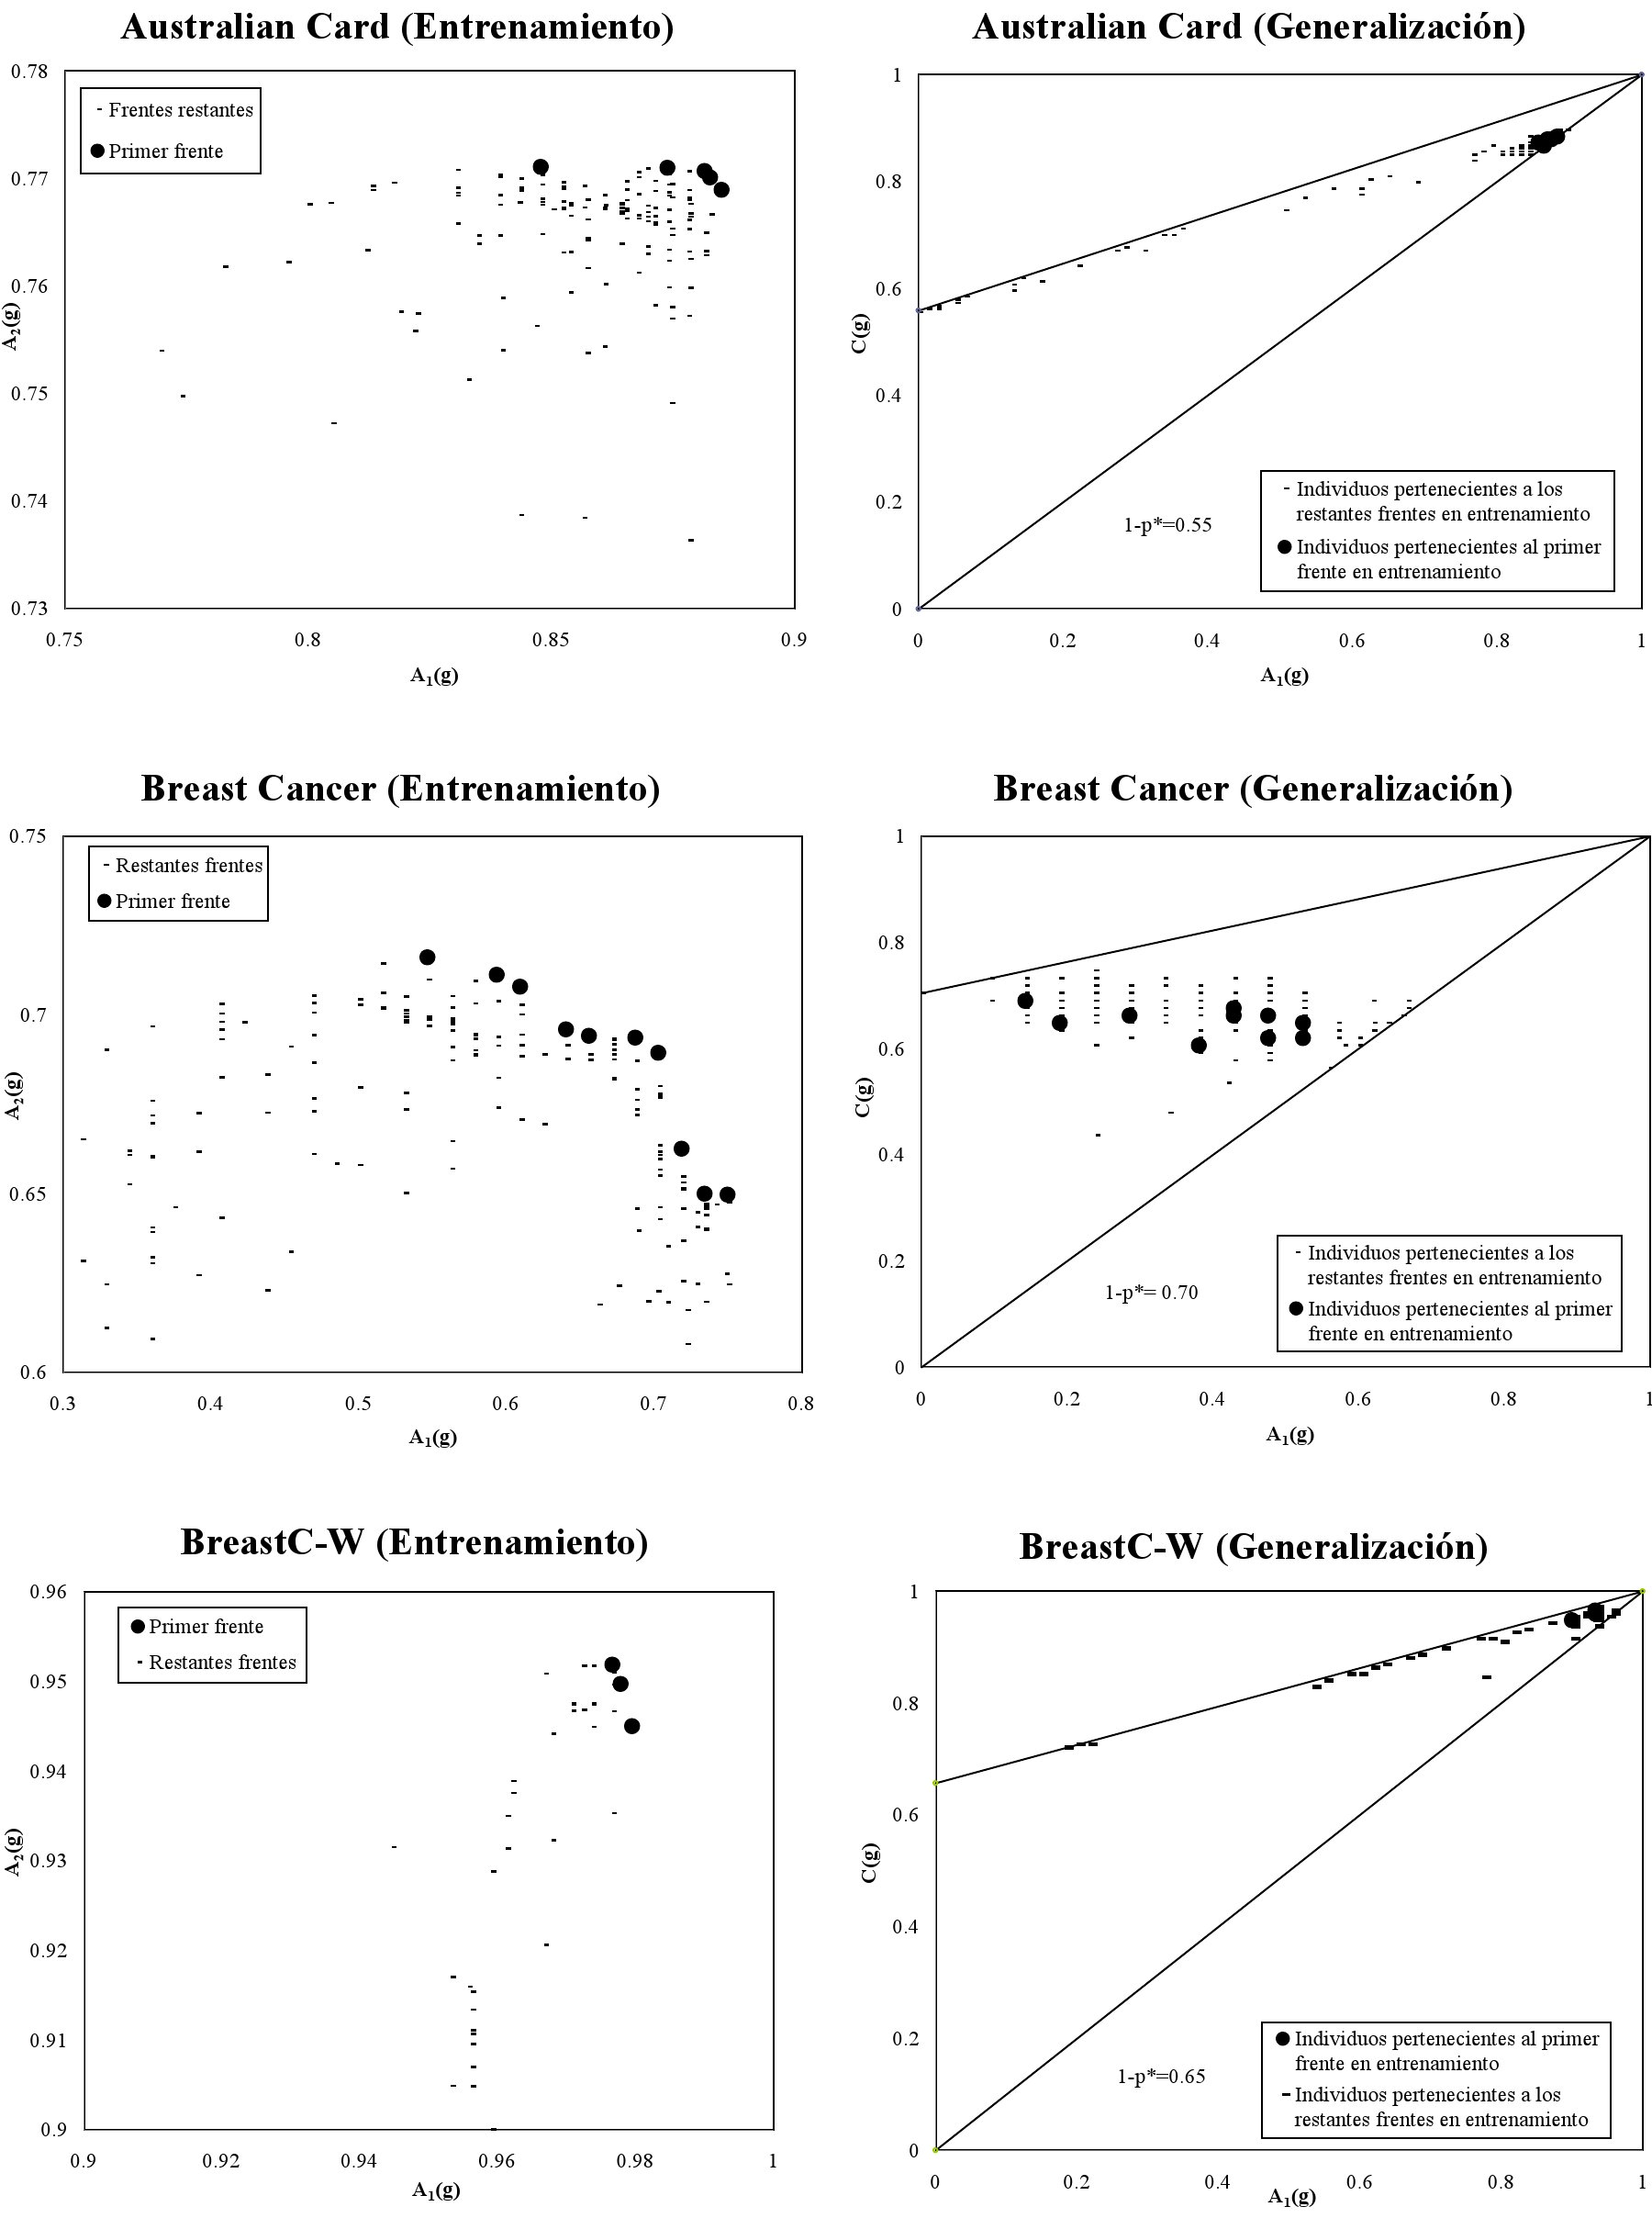
\includegraphics[keepaspectratio,width=13cm]{figuras/tanda1.jpg}
\caption{Frente de Pareto en entrenamiento $(A_{1},A_{2})$, y valores asociados a
$(A_{1},C)$ en generalización para los conjuntos Australian Card, Breast Cancer y
Breast Cancer Wisconsin.}
\label{tanda1}
\end{figure}

\begin{figure}[!htb]
\centering
	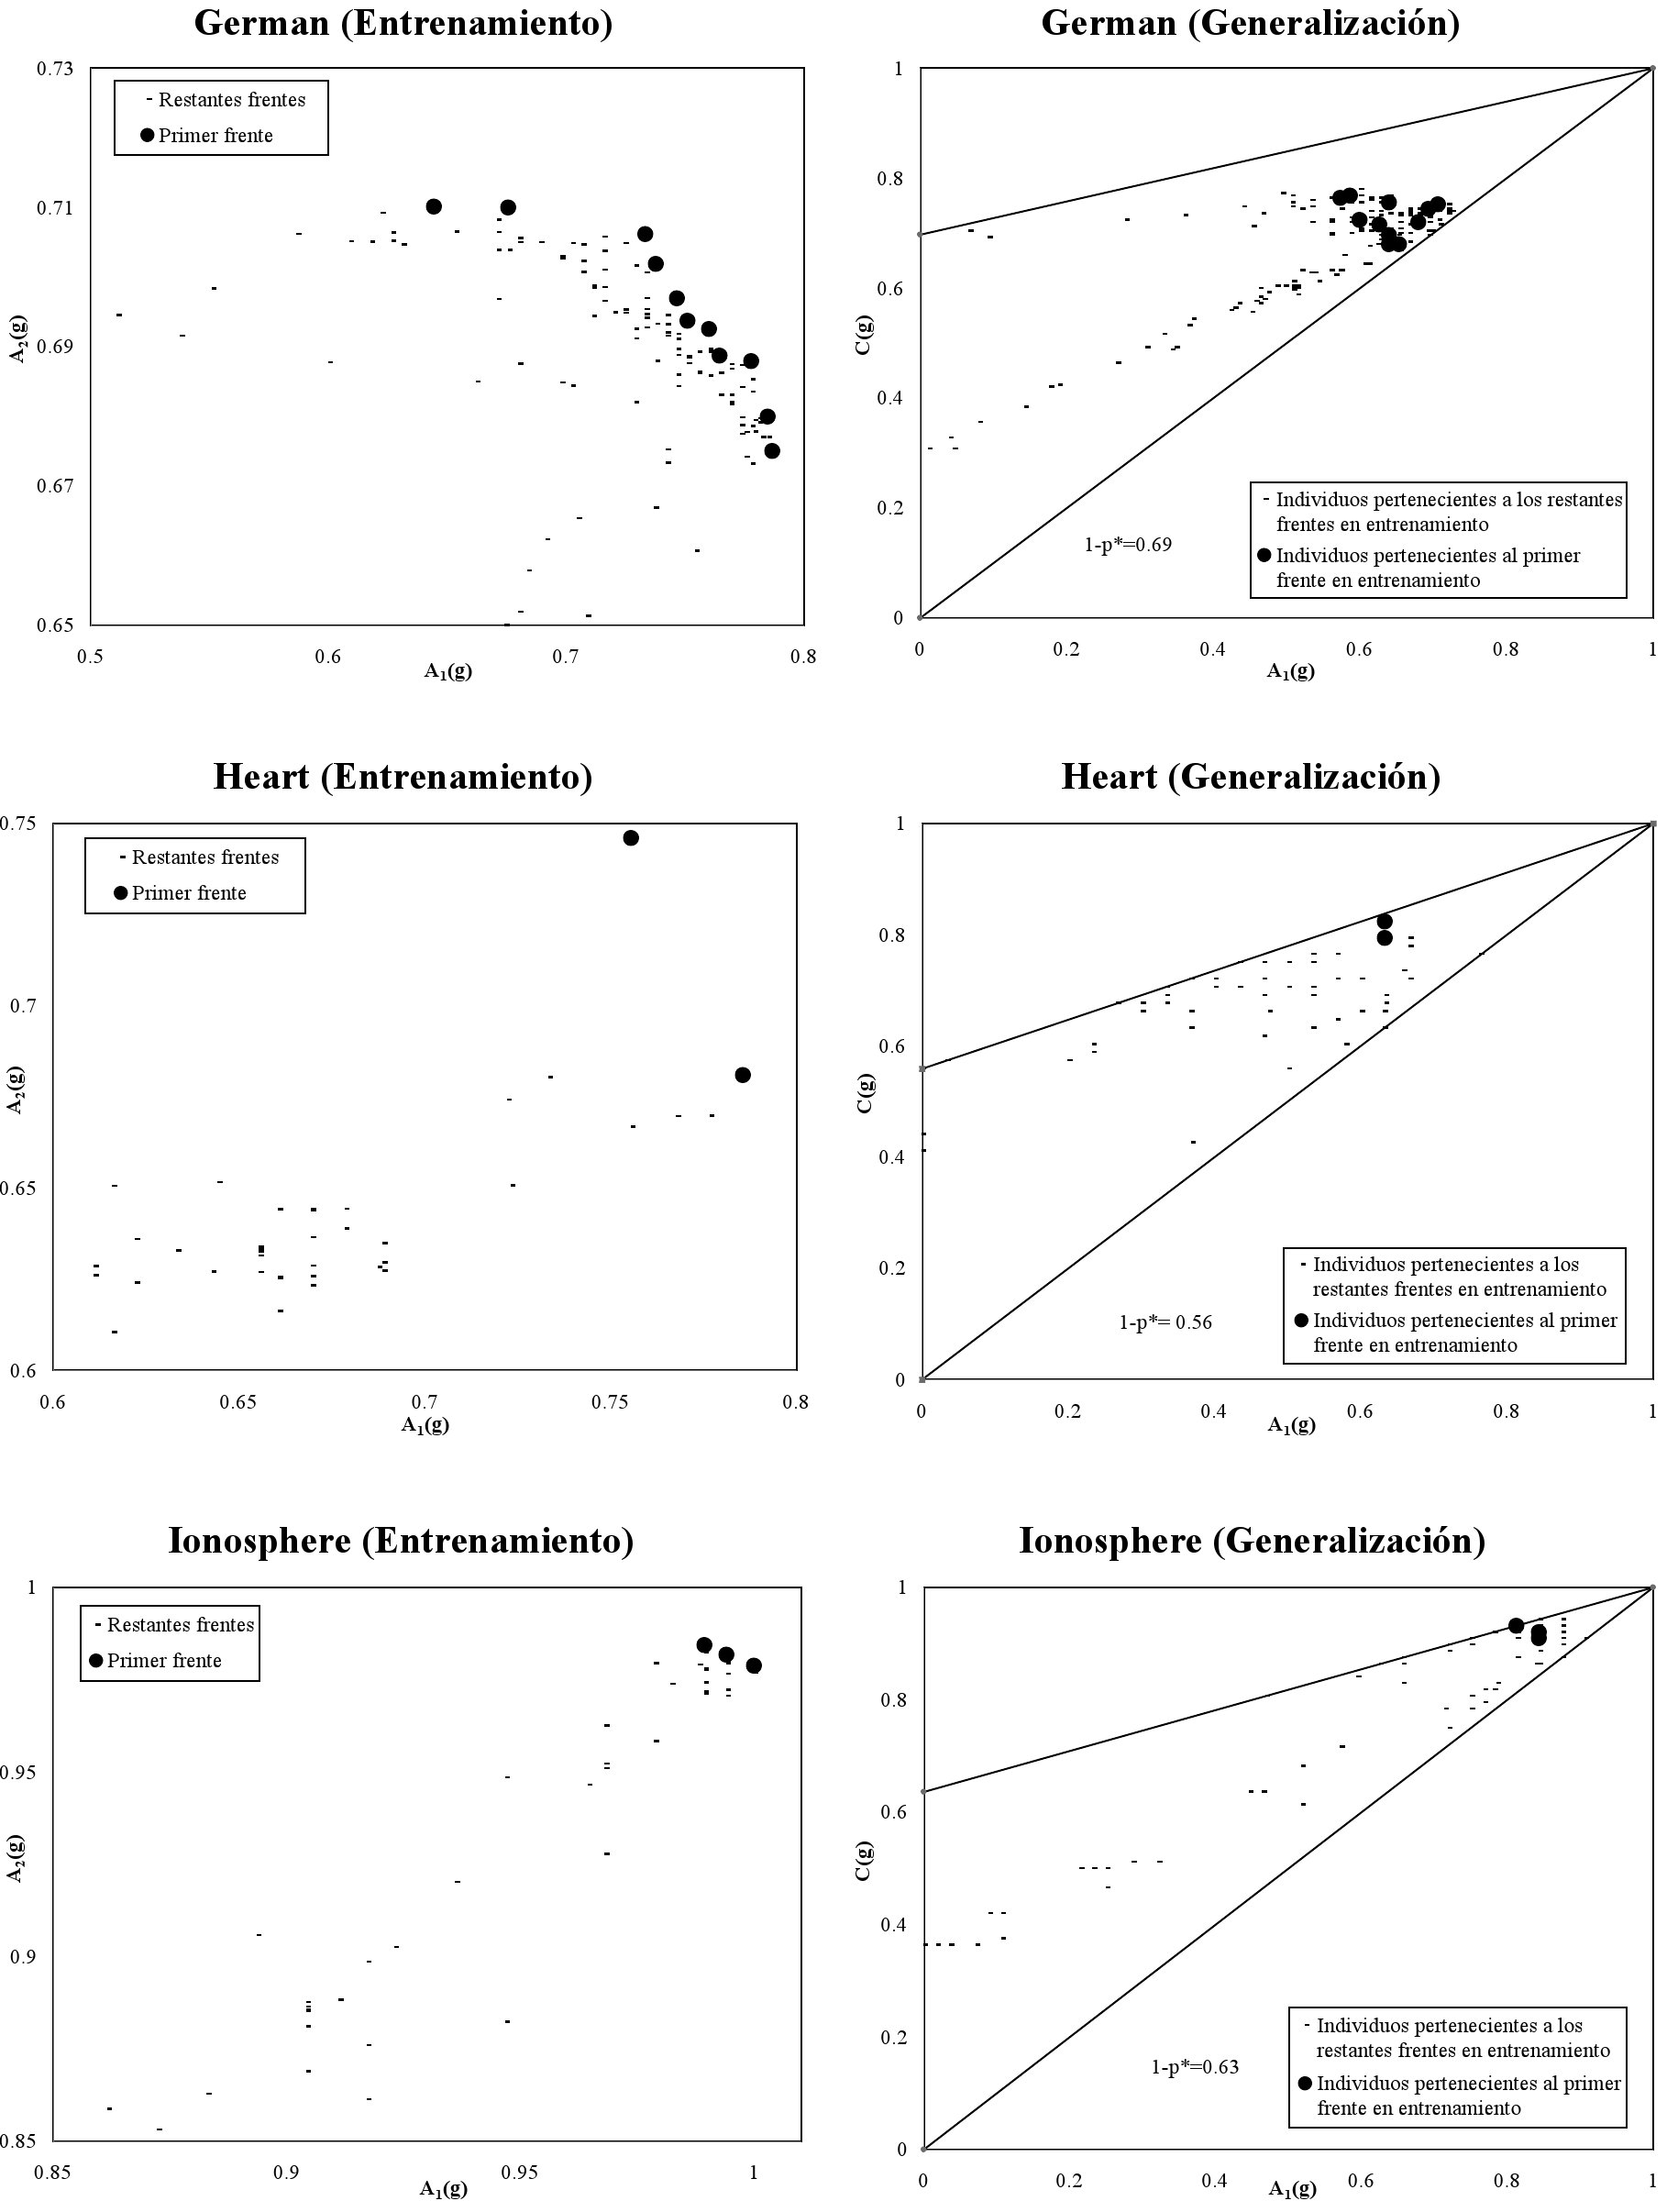
\includegraphics[keepaspectratio,width=13cm]{figuras/tanda2.jpg}
\caption{Frente de Pareto en entrenamiento $(A_{1},A_{2})$, y valores asociados a
$(A_{1},C)$ en generalización para los conjuntos German, Heart e Ionosphere.}
\label{tanda2}
\end{figure}

\begin{figure}[!htb]
\centering
	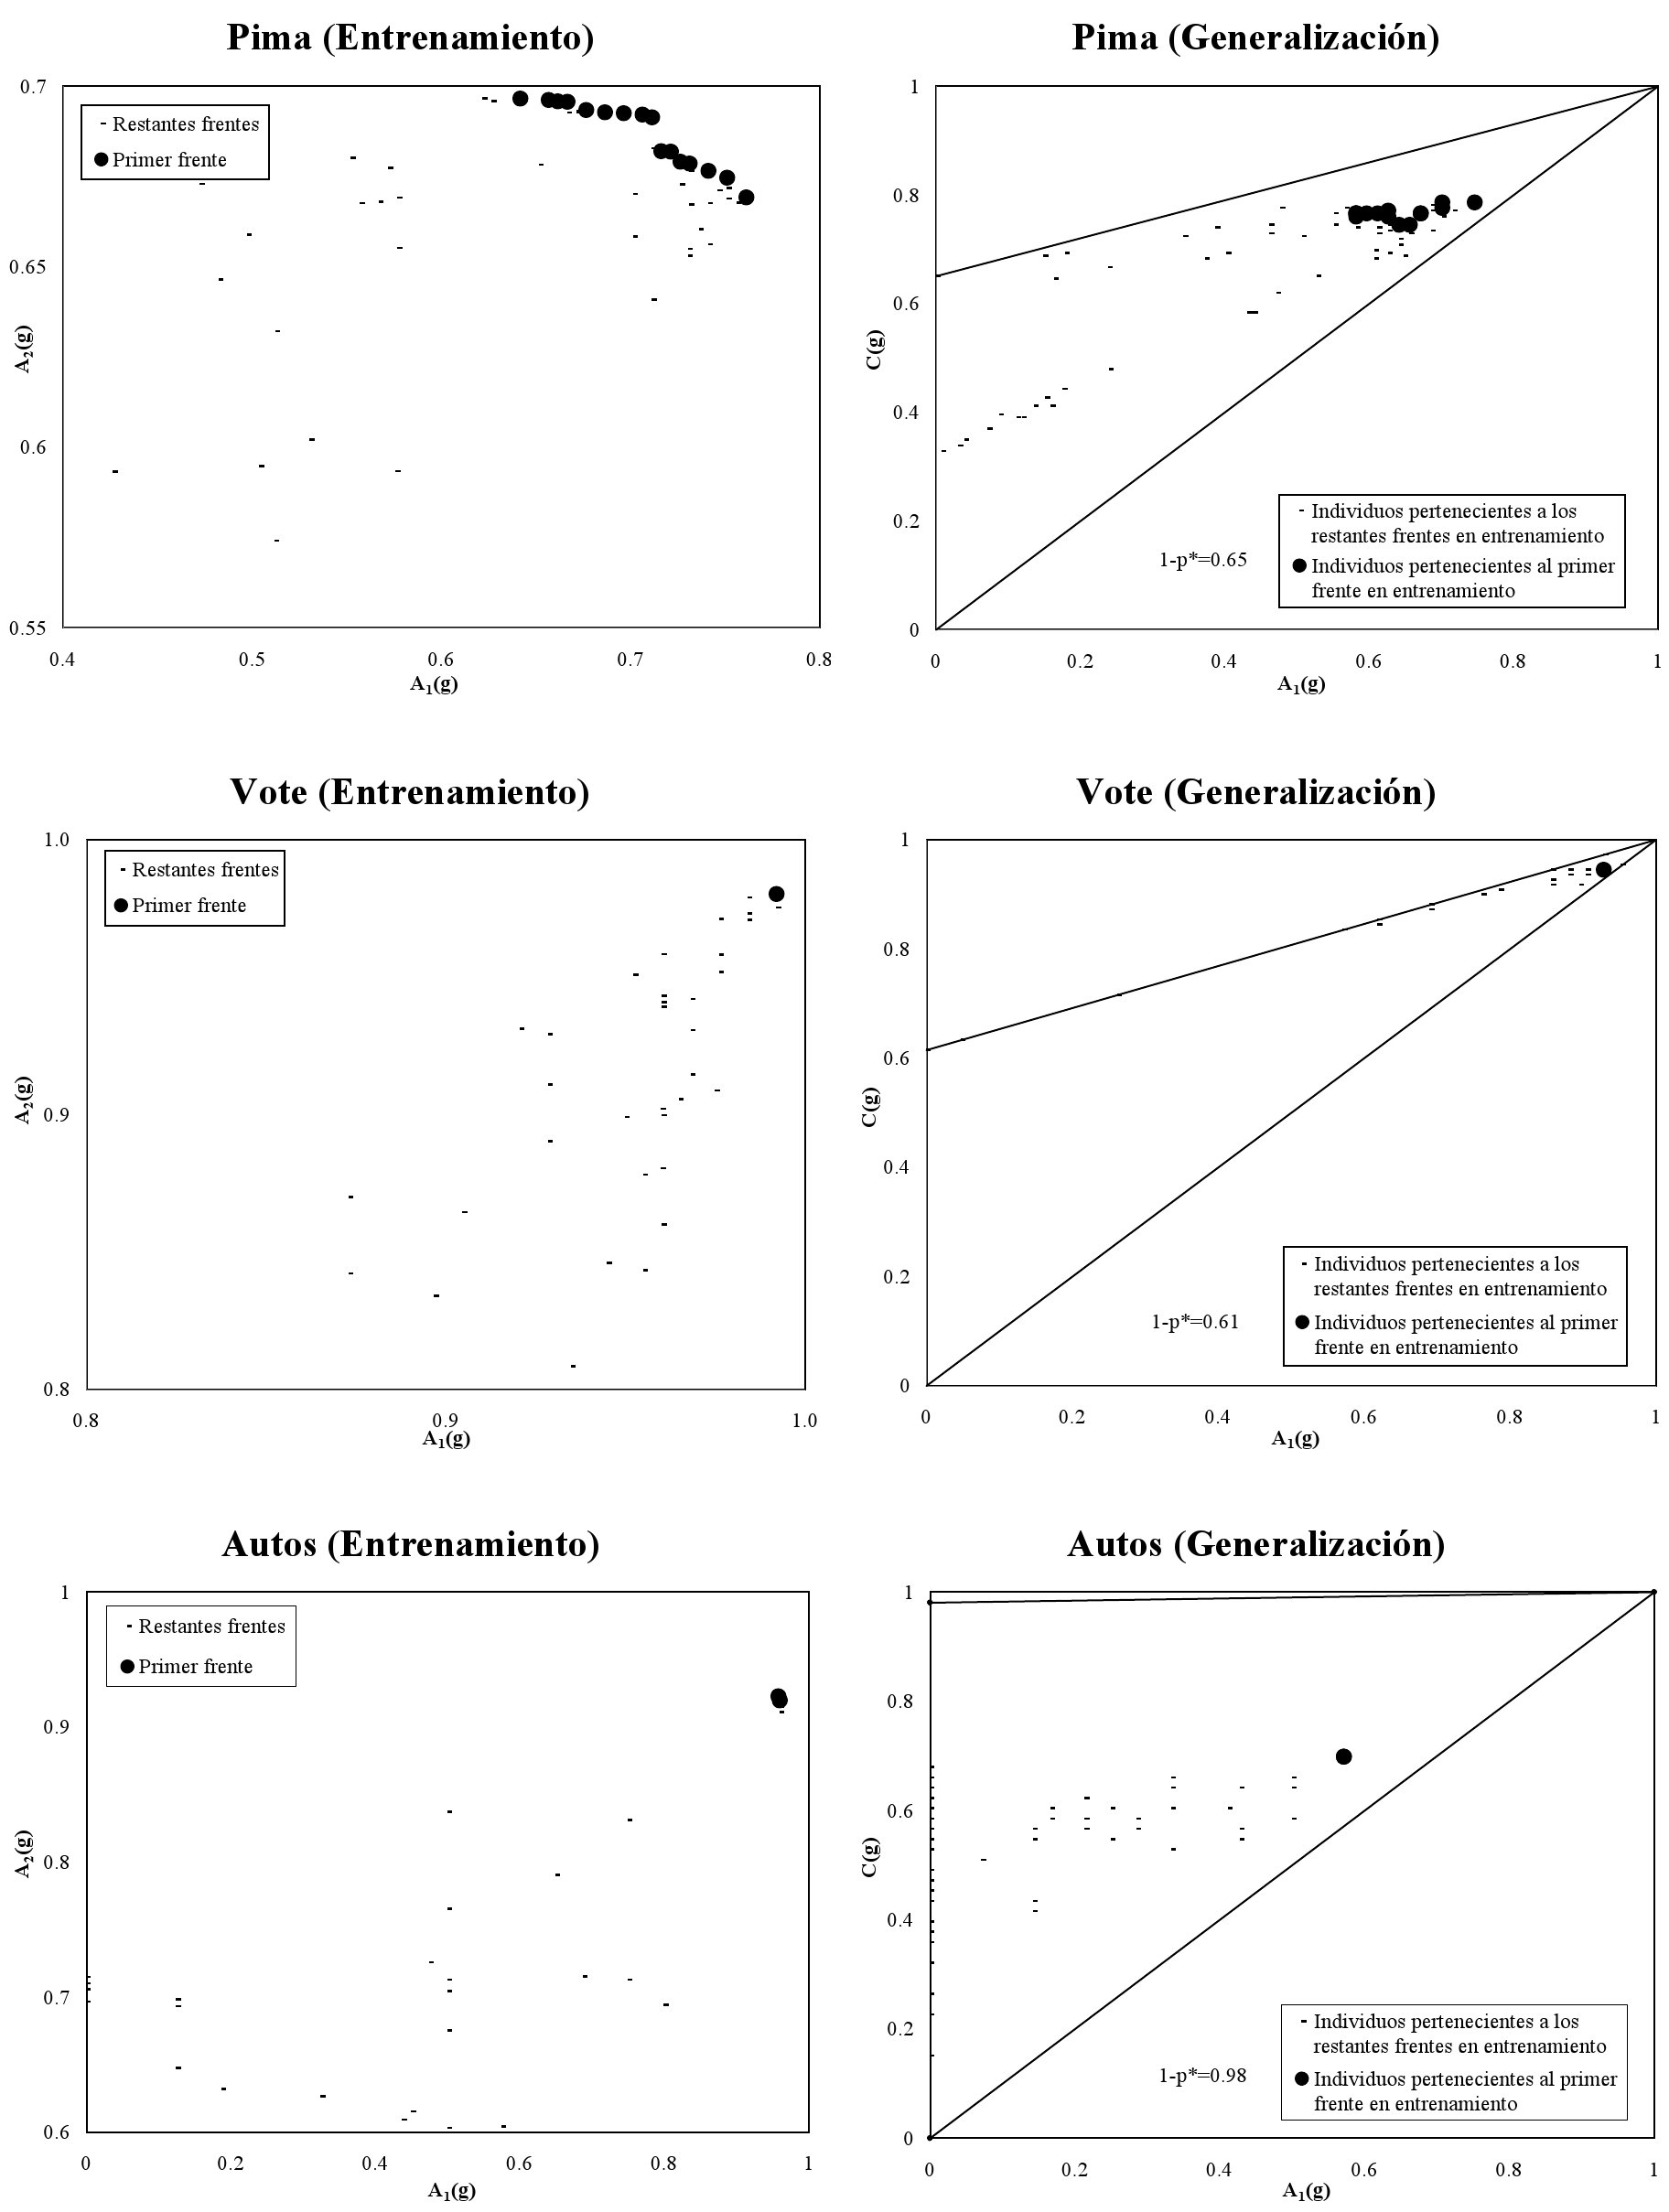
\includegraphics[keepaspectratio,width=13cm]{figuras/tanda3.jpg}
\caption{Frente de Pareto en entrenamiento $(A_{1},A_{2})$, y valores asociados a
$(A_{1},C)$ en generalización para los conjuntos Pima, Vote y Autos.}
\label{tanda3}
\end{figure}

\begin{figure}[!htb]
\centering
	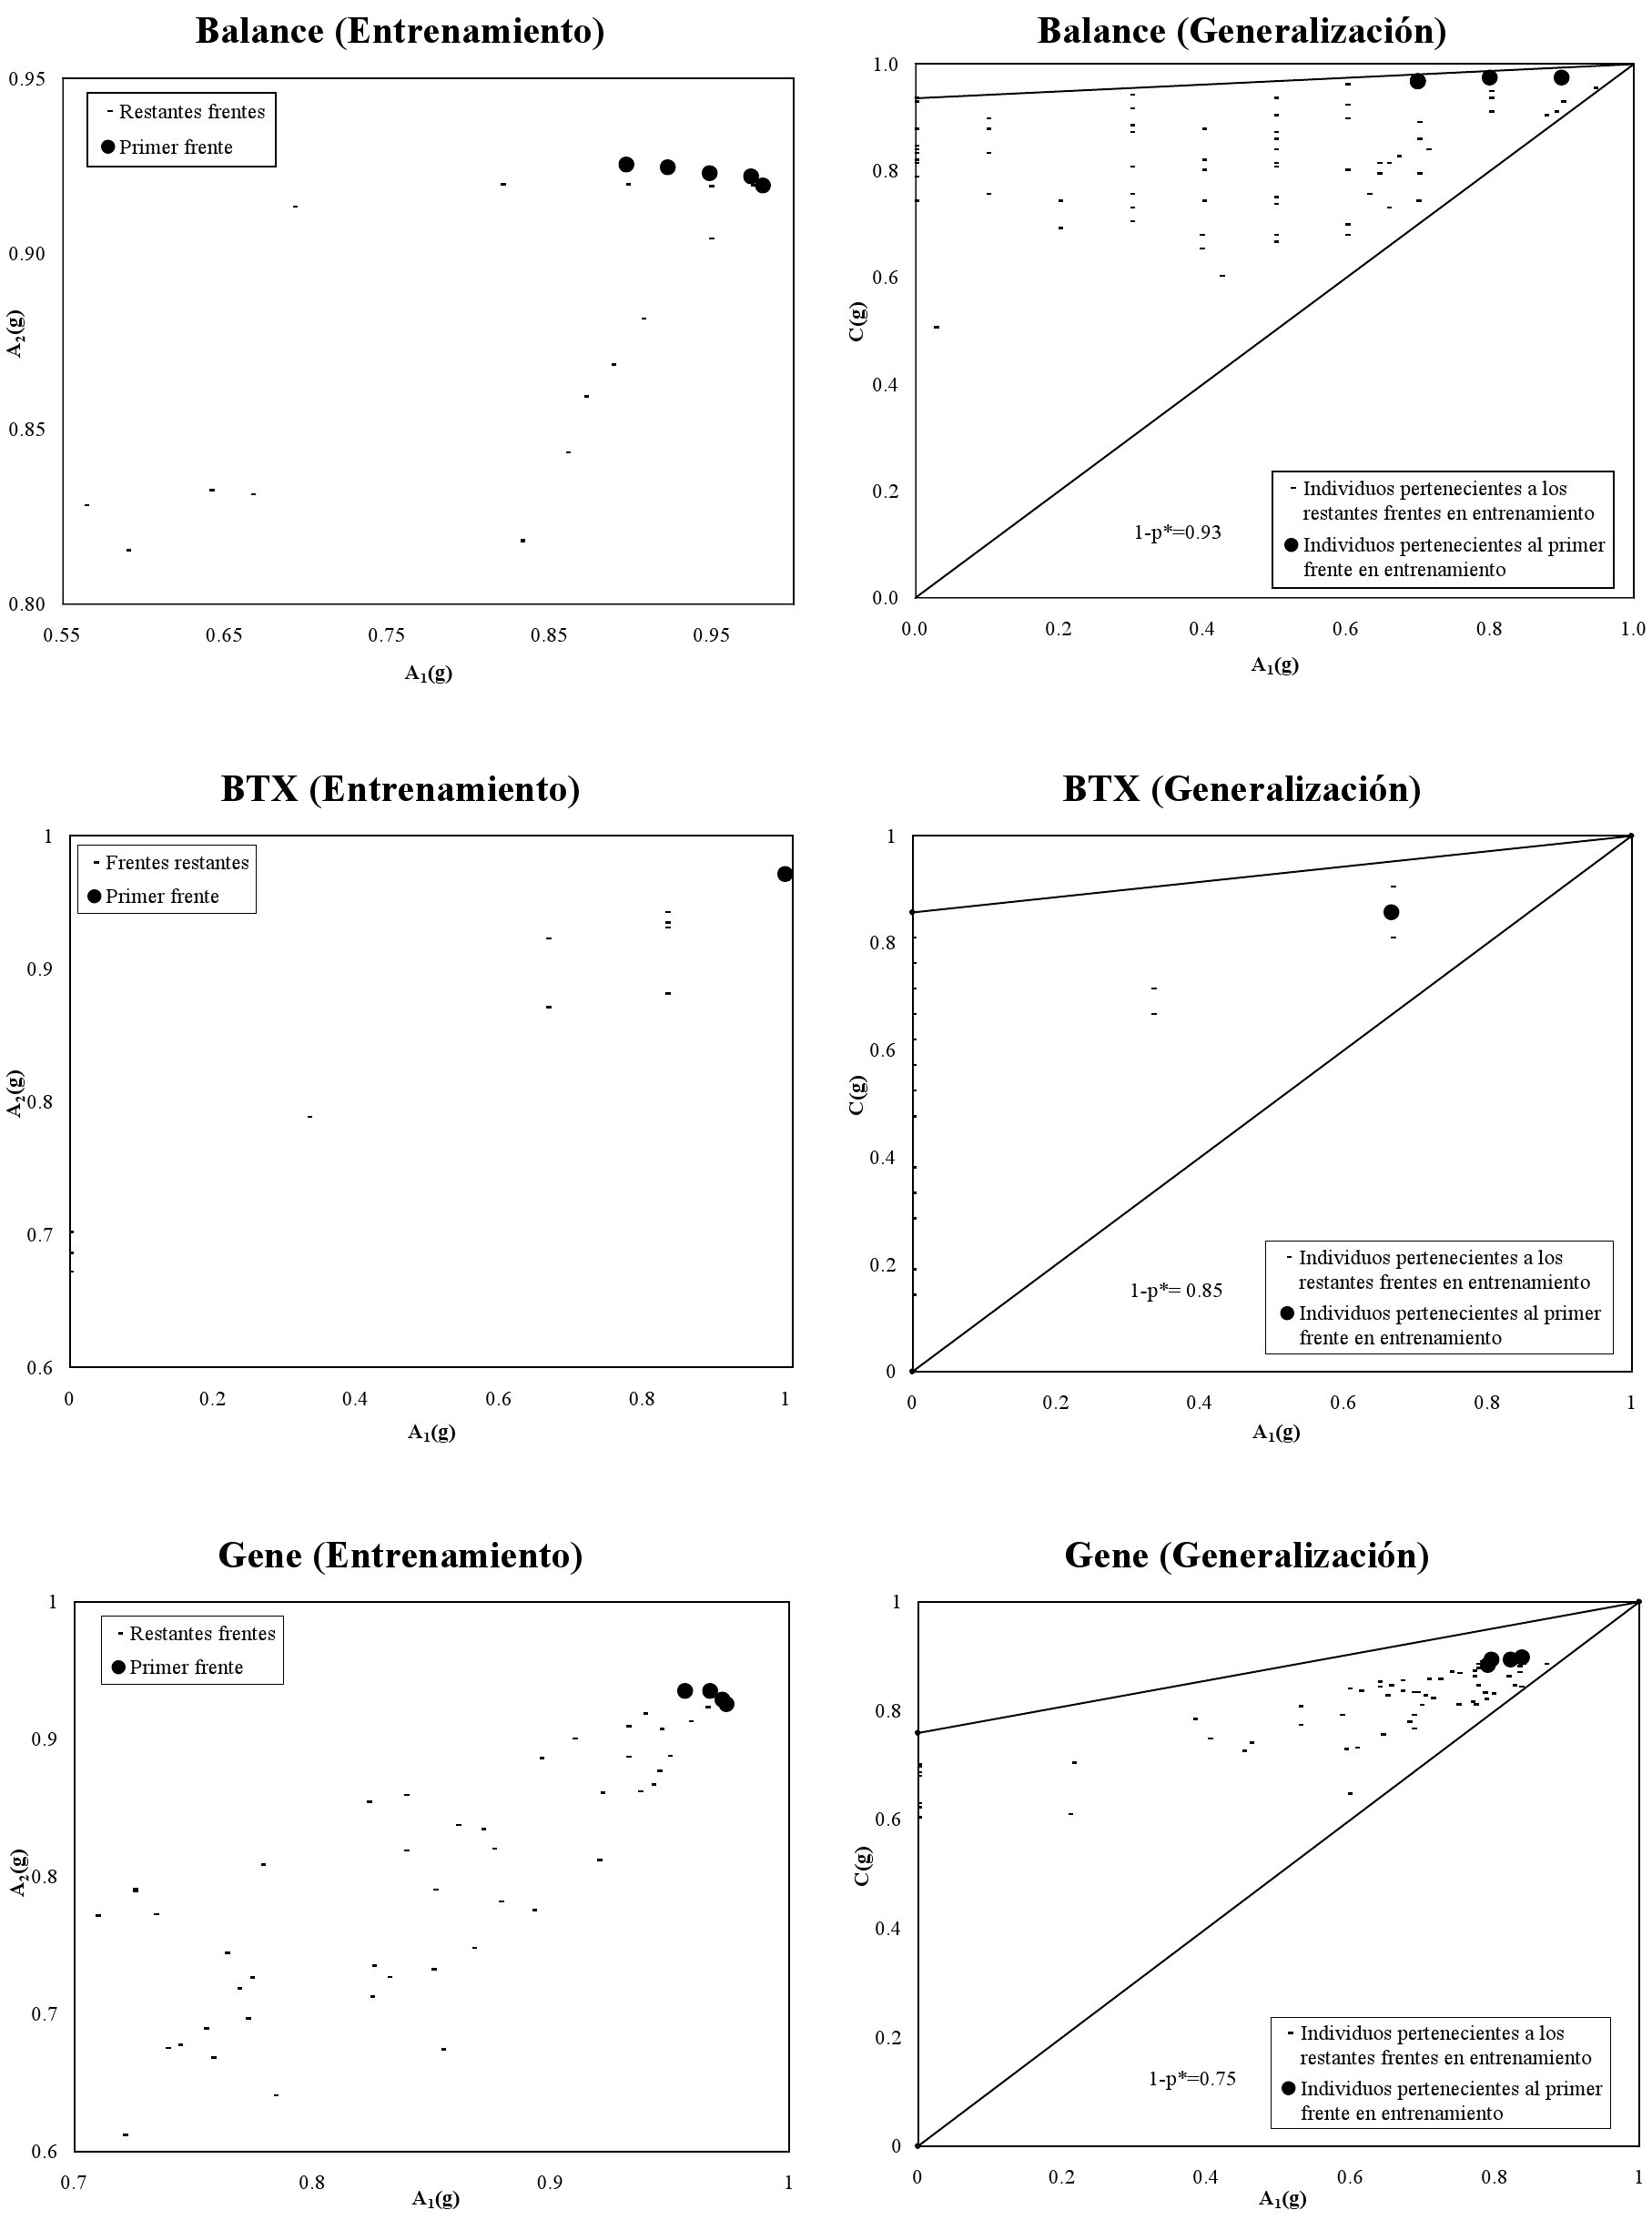
\includegraphics[keepaspectratio,width=13cm]{figuras/tanda4.jpg}
	\caption{Frente de Pareto en entrenamiento $(A_{1},A_{2})$, y valores asociados
a $(A_{1},C)$ en generalización para los conjuntos Balance, BTX y Gene.}
\label{tanda4}
\end{figure}

\begin{figure}[!htb]
\centering
	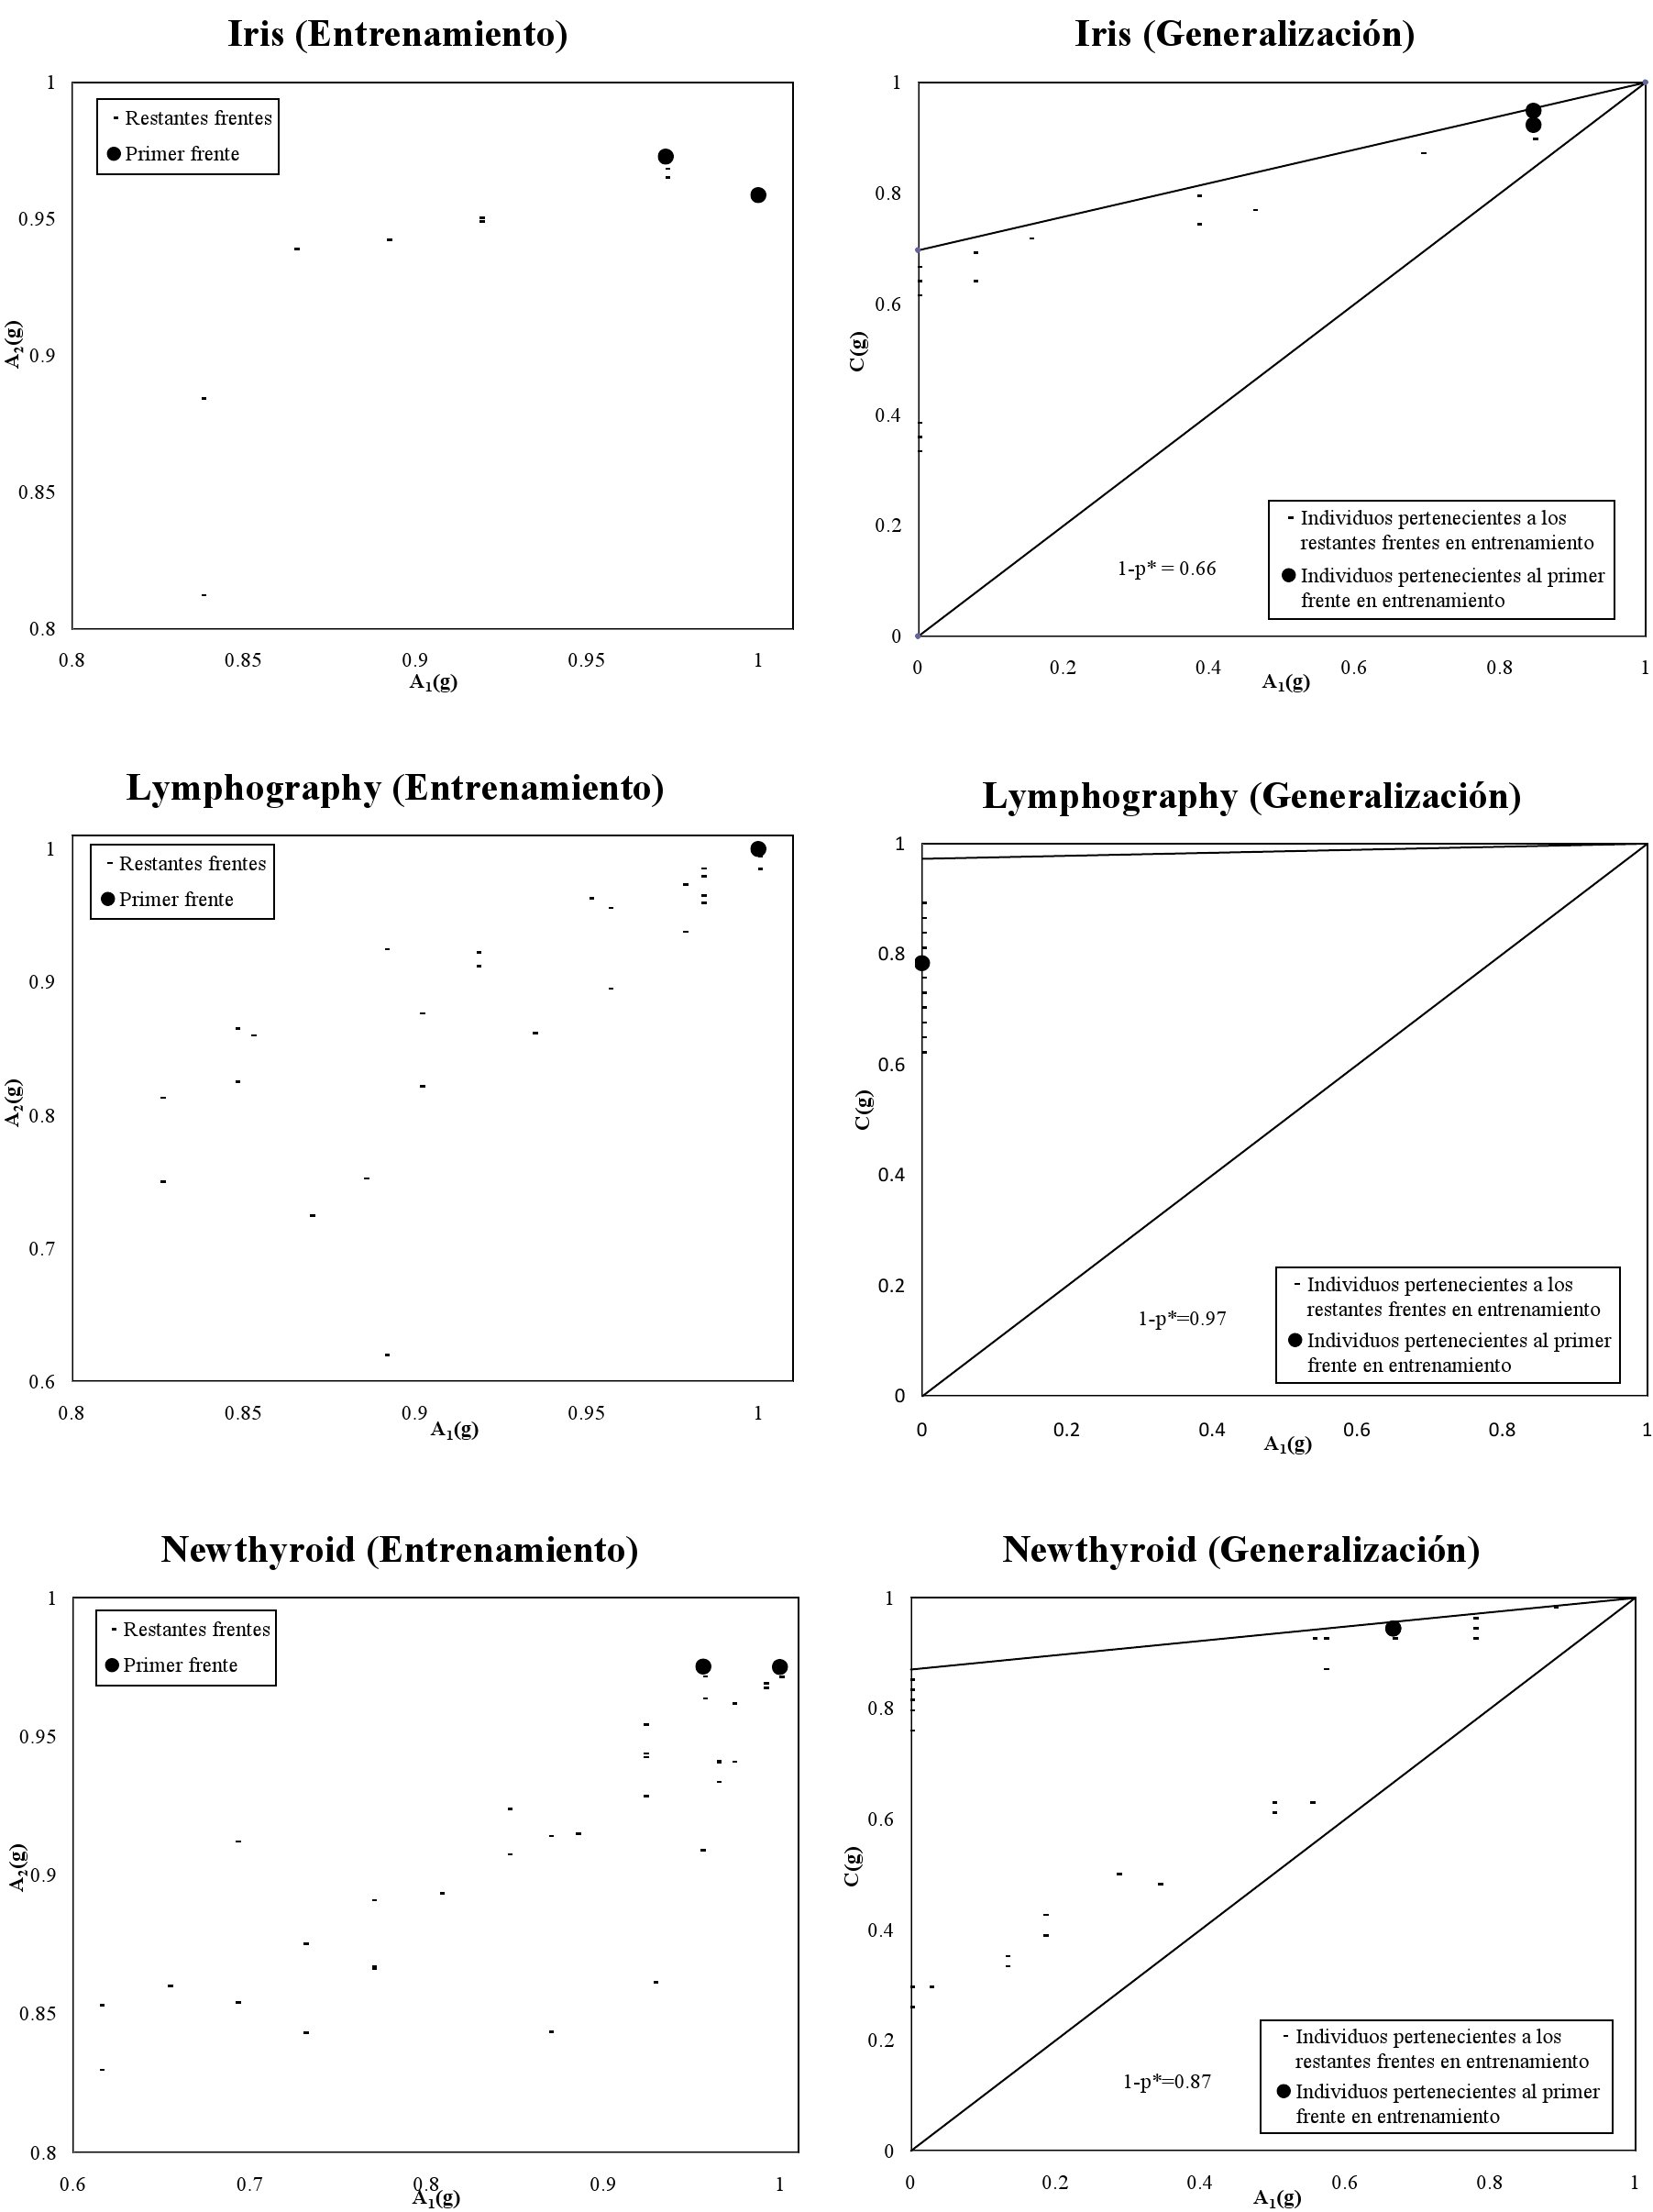
\includegraphics[keepaspectratio,width=13cm]{figuras/tanda5.jpg}
\caption{Frente de Pareto en entrenamiento $(A_{1},A_{2})$, y valores asociados a
$(A_{1},C)$ en generalización para los conjuntos Iris, Lymphography y Newthyroid.}
\label{tanda5}
\end{figure}

\begin{figure}[!htb]
\centering
	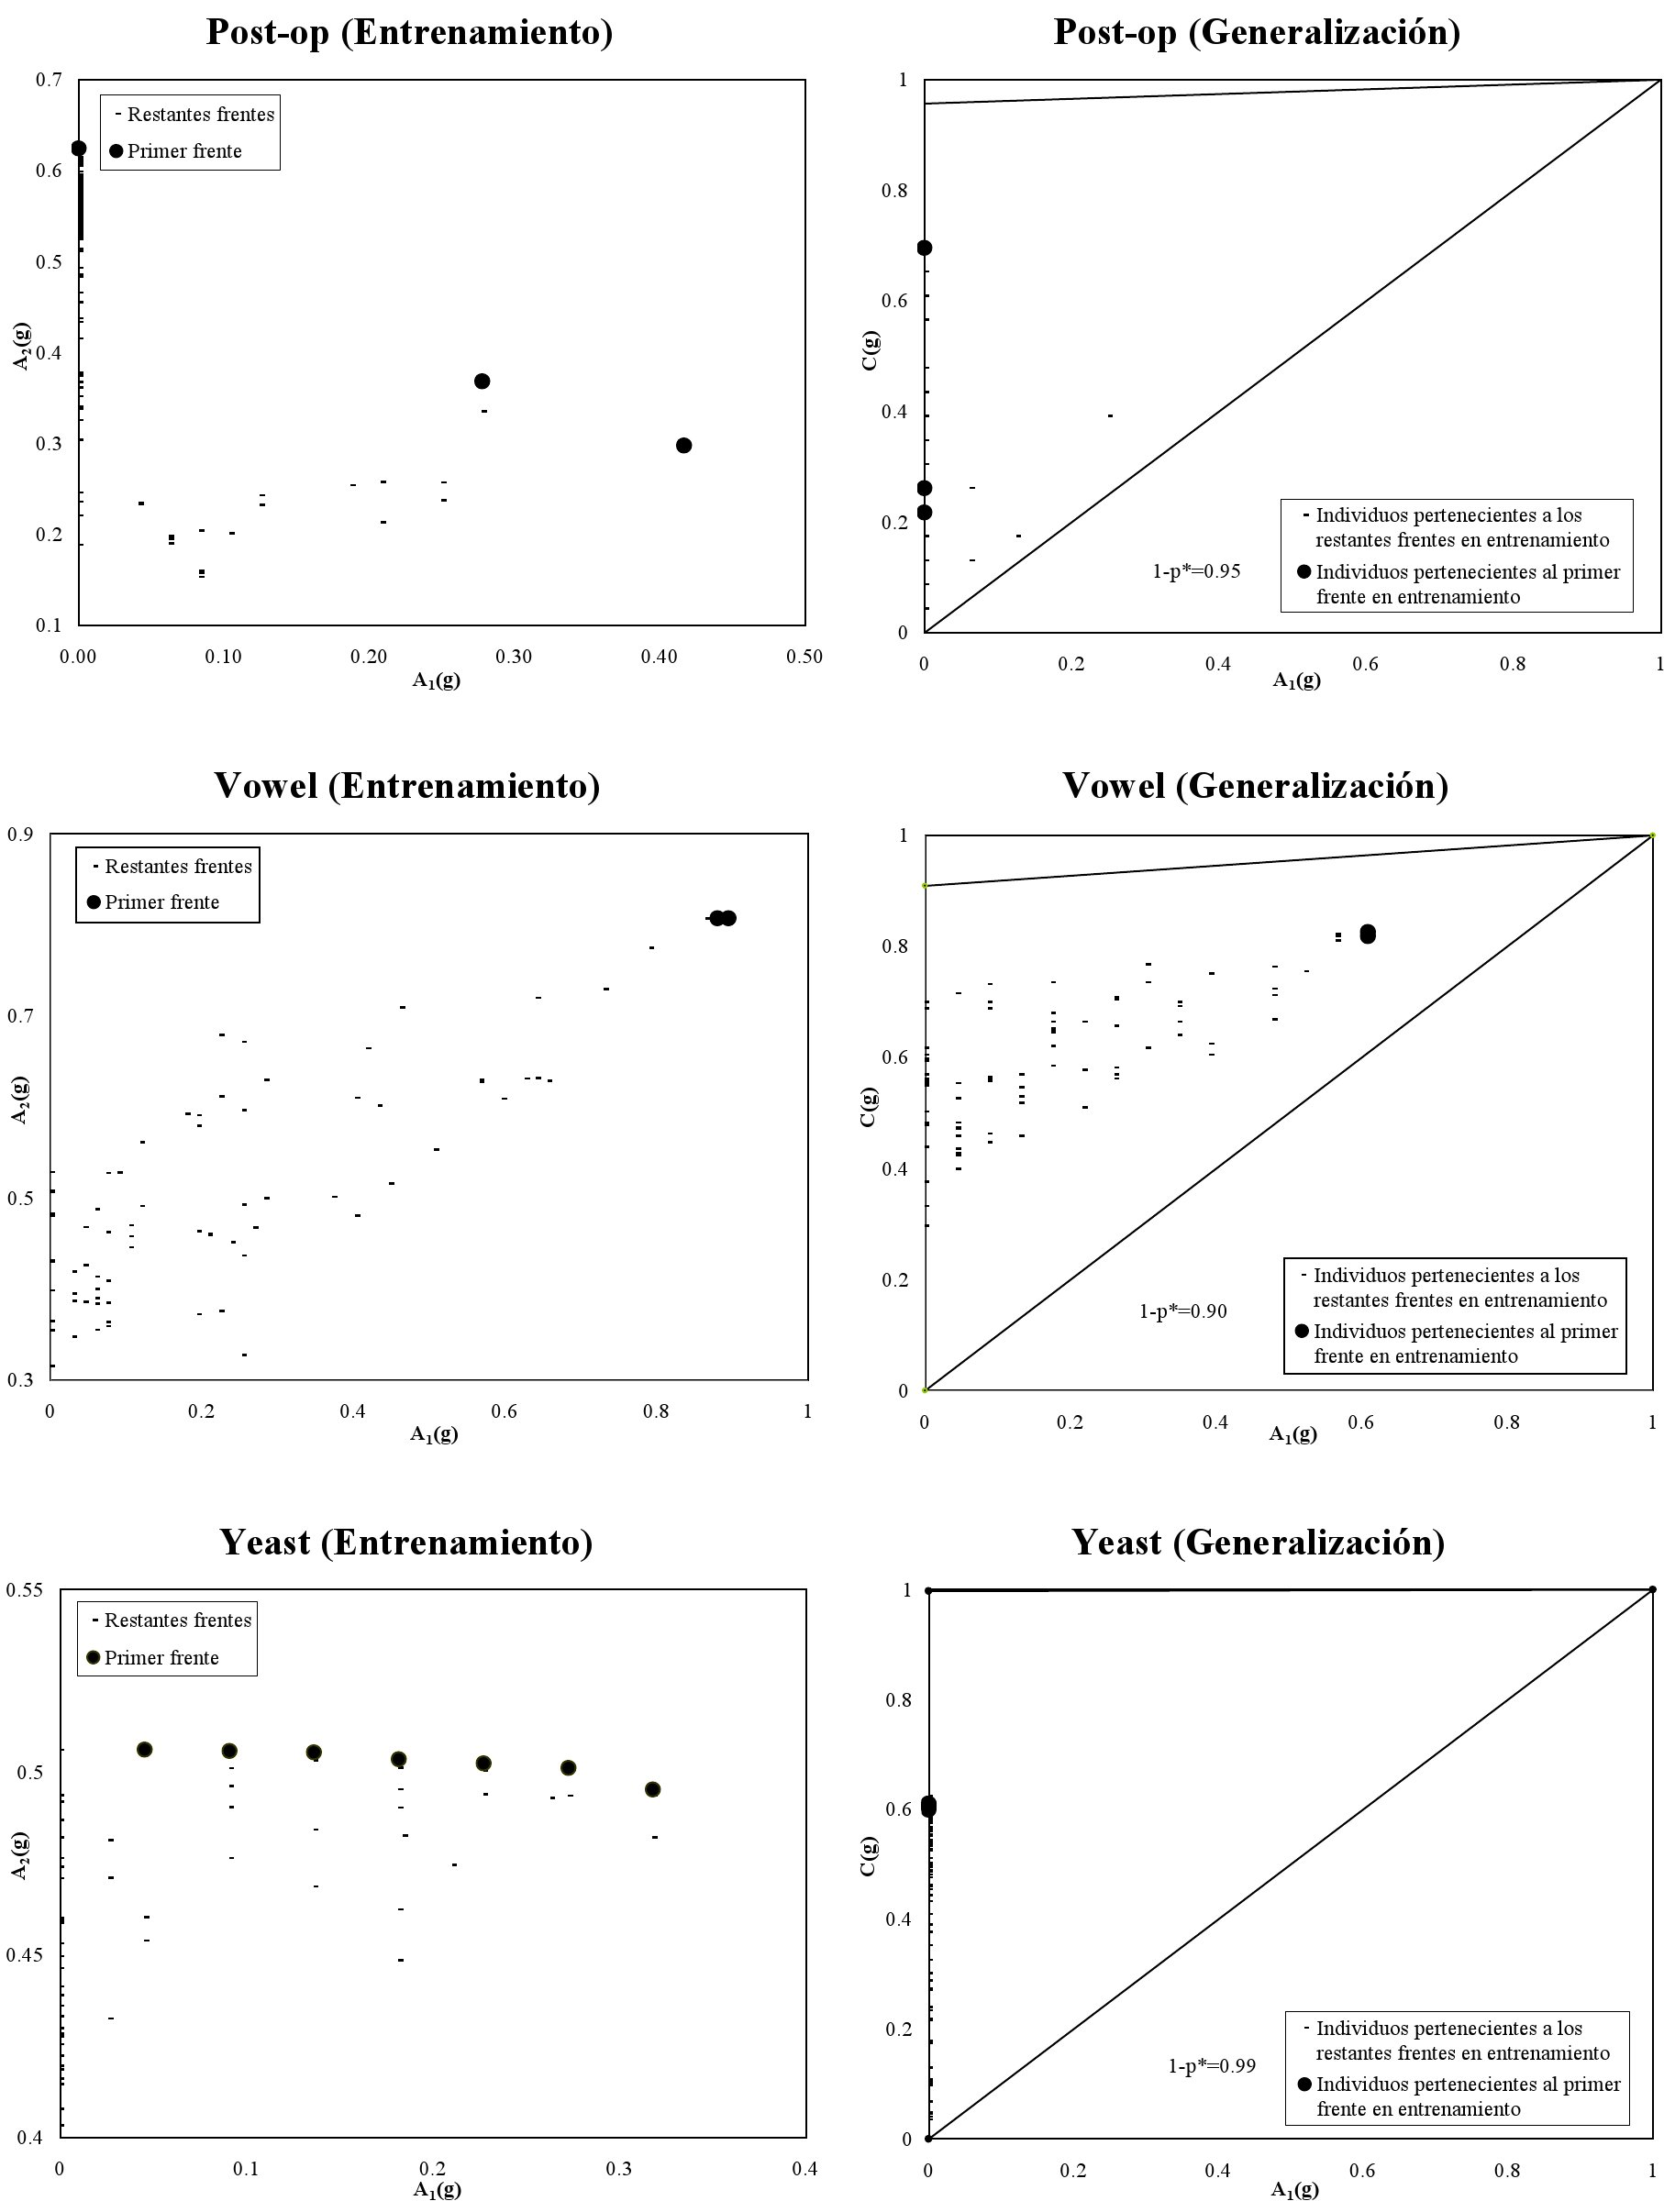
\includegraphics[keepaspectratio,width=13cm]{figuras/tanda6.jpg}
\caption{Frente de Pareto en entrenamiento $(A_{1},A_{2})$, y valores asociados a
$(A_{1},C)$ en generalización para los conjuntos Post-op, Vowel y Yeast.}
\label{tanda6}
\end{figure}

\clearpage
Finalmente, el lector puede observar en la figura \ref{ejemploPima}, como ejemplo, el
error
de $MS$ contra precisión para el algoritmo MPENSGAII en entrenamiento y
y en generalización, para el conjunto Pima. En dicha figura se puede ver
el frente de Pareto en entrenamiento y los valores asociados al plano $(MS,C)$ tanto en
entrenamiento como en generalización (en una de las 30 ejecuciones para ese
conjunto).

\begin{figure}[!htb]
\centering
\includegraphics[keepaspectratio,width=13cm]{figuras/ejemploPima.jpg}
\caption{Ejemplo de frente de Pareto en entrenamiento $(A_{1},A_{2})$, y valores asociados
a $(A_{1},C)$ en entrenamiento y generalización para el conjunto Pima en una
ejecución
concreta.}
\label{ejemploPima}
\end{figure}
\newpage
En la tabla \ref{tabla5MPENSGAII} mostramos los mejores modelos que se han
obtenido en entrenamiento para Pima (extremos del frente de Pareto) junto con el número de
neuronas, número de enlaces, los valores $A_{1}$, $A_{2}$, $MS$ y $C$ en entrenamiento y
los valores $MS$ y $C$ en generalización, para una ejecución de las 30, que como
siempre es la que presenta el mejor individuo en $E$. Un punto a destacar sobre
estos modelos es que el algoritmo MPENSGAII poda las conexiones, seleccionando las
variables más importantes para la clasificación. El modelo MPENSGAIIE presenta mayor
número de variables de entrada que el modelo MPENSGAIIS, por lo que el número de
conexiones es mayor, 39 para el primero y 26 para el segundo, aunque ambos necesitan 4
neuronas en la capa intermedia. Como se puede observar, el valor de $A_{1}$ en
entrenamiento para MPENSGAIIE (0.64) es menor que para MPENSGAIIS (0.76), y justo al
contrario pasa con el valor de $A_{2}$, siendo 0.69 para MPENSGAIIE y 0.66 para
MPENSGAIIS. Con respecto a los valores de $MS$ en entrenamiento, el modelo
MPENSGAIIE tiene un valor de $MS$ de 0.64 mientras que el modelo MPENSGAIIS tiene un valor
de 0.76, ya que este último modelo es del extremo inferior del frente de Pareto. En
cuanto al valor de $C$ en entrenamiento, el modelo MPENSGAIIE tiene una valor de 0.78
frente a un valor de 0.76 del modelo MPENSGAIIS, ya el el modelo MPENSGAIIE es del
extremo superior del frente de Pareto. Finalmente en generalización el modelo MPENSGAIIS
obtiene mejores valores tanto en $MS$ como en $C$, por lo que en este caso recomendamos ésta
metodología, ya que presenta valores de $MS_{G}=0.74$, frente a $MS_{G}=0.58$ para MPENSGAIIE,
siendo estos valores en $C_{G}$ similares.

\begin{landscape}
\begin{table}[!htb]
\scriptsize
\tabcolsep 15pt
\caption{Mejores modelos en entrenamiento para Pima en los extremos
del primer frente de Pareto obtenido con MPENSGAII, con sus correspondientes valores en
generalización.}
\label{tabla5MPENSGAII}
\begin{tabular}{>{\columncolor[rgb]{0.86,0.94,1}}p{2.2cm}>{\columncolor[rgb]{0.86,0.94,1}}
l}\hline
\rowcolor[rgb]{0.70,0.85,1}\textbf{Individuo} & \textbf{Modelo matemático} \\ \hline
& $DF_{E}=2.74 - 4.74B_{1}(\bar{x},\Theta) + 4.81B_{2}(\bar{x},\Theta) -
1.09B_{3}(\bar{x},\Theta)+4.04B_{4}(\bar{x},\Theta)$ \\
& \\
& $B_{1}(\bar{x},\Theta)= (1/(1+\exp\left\lbrace
-(+1.07x_{1}+0.66x_{2}+0.43x_{3}-0.42x_{5}+5.89x{6}-2.92x_{7}+0.06x_{8}+0.69)
\right\rbrace))$\\
& $B_{2}(\bar{x},\Theta)= (1/(1+\exp\left\lbrace-(-0.17x_{1}-4.02x_{2}+1.07x_{3}+0.72x_{4}
+0.14x_{5}+1.22x_{6}-4.15x_{7}-2.96x_{8}-3.08)\right\rbrace))$ \\
& $B_{3}(\bar{x},\Theta)=
(1/(1+\exp\left\lbrace-(+0.62x_{1}+0.64x_{2}+0.24x_{3}-0.02x_{4}-0.02x_{5}+6.
22x_{6}+1.06x_{7}+0.07x_{8}+1.95)\right\rbrace))$ \\
& $B_{4}(\bar{x},\Theta)=
(1/(1+\exp\left\lbrace-(+0.70x_{1}-0.57x_{2}-0.57x_{3}-0.52x_{4}-1.08x_{5}-1.
87x_{6}+4.87x_{8}-2.84)\right\rbrace))$ \\
& \\
& $A_{1}(g)=0.64$; $A_{2}(g)=0.69$; $MS_{{\rm T}}=0.64$; $C_{{\rm T}}=0.78$; $MS_{{\rm
G}}=0.58$; $C_{{\rm G}}=0.76$;\\
\multirow{-8}{2.2cm}{Mejor individuo en el plano $(A_{1},A_{2})$ considerando $A_{2}$
(MPENSGA2E)}& neuronas = 4; conexiones efectivas = 39\\ \hline
& $DF_{MS}=2.77- 4.76B_{1}(\bar{x},\Theta) +
4.74B_{2}(\bar{x},\Theta)-1.09B_{3}(\bar{x},\Theta)+3.12B_{4}(\bar{x},\Theta)$\\
& \\
& $B_{1}(\bar{x},\Theta)=(1/(1+\exp\left\lbrace-(+4.41x_{6}-2.98x_{7}
+0.97(1))\right\rbrace))$\\
& $B_{2}(\bar{x},\Theta)=
(1/(1+\exp\left\lbrace-(+0.20x_{1}-4.73x_{2}+1.03x_{4}+0.10x_{5}-2.89x_{6}
-4.55x_{7}-3.27x_{8}-3.01(1))\right\rbrace))$ \\
& $B_{3}(\bar{x},\Theta)=(1/(1+\exp\left\lbrace-(-0.07x_{2}+0.13x_{4}+0.77x_{6}
+1.13x_{7}+0.07x_{8}+1.89(1))\right\rbrace))$\\
&$B_{4}(\bar{x},\Theta)=(1/(1+\exp\left\lbrace-(+0.24x_{1}-0.26x_{7}+6.69x_{8}
-2.66(1))\right\rbrace))$\\
& \\
& $A_{1} (g)=0.76$; $A_{2} (g)=0.66$; $MS_{{\rm T}}=0.76$; $C_{{\rm T}}=0.76$;
$MS_{{\rm G}}=0.74$; $C_{{\rm G}}=0.78$;\\
\multirow{-8}{2.2cm}{Mejor individuo en el plano $(A_{1},A_{2})$ considerando $A_{1}$
(MPENSGA2S)} & neuronas = 4; conexiones efectivas = 26\\ \hline
\multicolumn{2}{l}{DF=Función discriminante.}\\
\end{tabular}
\end{table}
\end{landscape}

A modo de resumen y conclusión, la metodología MPENSGAII propone una nueva aproximación
en problemas de clasificación multi-clase basada en una medida de rendimiento
bidimensional, $MS$ y $C$. Los resultados muestran
que con estas medidas es posible obtener clasificadores que combinen un nivel alto de
clasificación con un buen nivel de clasificación por clase.

Una de las áreas que mas auge ha tenido en los últimos años dentro del
aprendizaje automático es aquella en donde se combinan las decisiones de clasificadores
individuales, con la finalidad de que la decisión final de a qué clase pertenece un
ejemplo se realice por un conjunto de clasificadores, a los que se les suele
llamar \textit{ensemble} \cite{Dietterich1997,Kuncheva2005}.

\section{\textit{Ensembles} de clasificadores}\label{introEnsembles}
\noindent Cuando se habla de \textit{ensembles} es necesario distinguir entre: la manera
de generar clasificadores, la manera de elegir qué clasificadores de entre los que
disponemos y cuáles de ellos formarán el \textit{ensemble} (ligado al concepto de
diversidad),
y finalmente, las reglas o formas de utilizar el \textit{ensemble} para clasificar a un
determinado patrón o instancia. Dependiendo de lo que se tenga en cuenta, hay autores que
hacen una taxonomía de \textit{ensembles} diferente. El lector puede consultar un extenso
estado del arte, referencias bibliográficas y taxonomías para la formación de
\textit{ensembles} en tareas de clasificación en \cite{Rokach2009}.

Siguiendo el trabajo de Rokach \cite{Rokach2009}, los aspectos a
tener en cuenta en la creación de un \textit{ensemble} son:
\begin{description}
	\item[$\blacktriangleright$ Uso del combinador:] Se entiende por combinador al proceso
de combinar las
clasificaciones arrojadas por varios clasificadores que forman un \textit{ensemble} para
obtener una conclusión, decisión, o clasificación final.

Existen, de manera general, dos métodos de combinación:
\begin{enumerate}
	\item \textbf{Métodos de pesos o de ponderación:} Estos métodos son más adecuados para
problemas en los que cada uno de los clasificadores realizan la misma tarea y tienen un
éxito equiparable, o cuando nos gustaría evitar problemas asociados al sobre-aprendizaje.
Suelen utilizar ponderaciones de las probabilidades de salida o de las asignaciones que
realiza cada clasificador a un determinado patrón para obtener la decisión final. Ejemplos
de esté tipo de técnicas (ver \cite{Rokach2009}) son: la mayoría de votos
(\textit{Majority
Voting}), la ponderación por rendimiento (\textit{Performance Weighting}), la distribución
de sumas o media simple (\textit{Distribution Summation} or \textit{Simple Averaging}), el
ganador lo consigue todo (\textit{Winner Takes All}) \cite{Theodoridis2006} (esta último
método no se cuentra en \cite{Rokach2009}), el método de \textit{Dempster-Shafer}, o el
método de
Naive Bayes.

	\item \textbf{Métodos de meta-aprendizaje:} Los métodos de meta-aprendizaje son más
convenientes para casos en los que determinados clasificadores cometen
errores de manera consistente en determinadas instancias. El aprendizaje se produce a
partir de los clasificadores inducidos y a partir de las clasificaciones de éstos
clasificadores en el conjunto de entrenamiento. Es decir, de alguna manera se introduce
un meta-aprendizaje a partir de los resultados que proporcionan algunos clasificadores
del \textit{ensemble} para proporcionárselos a otros, utilizando o no divisiones del
conjunto de entrenamiento inicial o mediante combinación de éste con las salidas de
clasificadores previos. Suele hacerse un aprendizaje por etapas. Ejemplos de estos
métodos (ver \cite{Rokach2009}) son \textit{Stacking}, \textit{Arbiter Trees},
\textit{Combiner Trees}, \textit{Grading}, \textit{Adaptive fusion and co-operative
training} y \textit{Mathematical Programming}.

La mayoría de los métodos de combinación no tienen en cuenta si los clasificadores son
dependientes o independientes (detallado a continuación). De esta manera, cuando los
clasificadores son dependientes, el rendimiento de los métodos de combinación se degrada,
sugiriéndose en la literatura varias técnicas para evitar el descenso de rendimiento
\cite{Rokach2009}, como por ejemplo transformar las salidas de los clasificadores a
medidas de confianza, de forma tal que cada transformación sea la combinación de una
función escalar y de un tipo de confianza \cite{Liu2005}.
\end{enumerate}
\item[$\blacktriangleright$ Dependencia de los clasificadores:] Se refiere a la manera
en la que se entrenan
los clasificadores que formarán un \textit{ensemble}, y de cómo un clasificador puede
afectar a otro en la decisión final. Así, los clasificadores pueden ser dependientes
o independientes.

En un marco \textbf{dependiente}, el resultado de un clasificador afecta a la
creación del siguiente, de manera que hay interacción en el proceso de aprendizaje. De
esta manera se puede utilizar el conocimiento generado en iteraciones previas para guiar
el aprendizaje de futuras iteraciones. Hay dos aproximaciones \cite{Rokach2009} relacionas
con la creación de clasificadores dependientes:
\begin{enumerate}
\item \textbf{Modelos guiados por selección de instancias:} En esta aproximación
los clasificadores se construyen mediante una serie de iteraciones previas, las cuales se
utilizan para cambiar el conjunto de entrenamiento para las siguientes iteraciones.
Estos métodos suelen ignorar las instancias que están bien clasificadas por los
clasificadores en pasos anteriores. Un ejemplo de este tipo de métodos, a los que se les
suelen llamar métodos de \textit{Boosting} (también se nombran por métodos de
\textit{Resampling} o \textit{Combining}), es el algoritmo AdaBoost y su
multitud de variantes \cite{Rokach2009}.
\item \textbf{Aprendizaje incremental por lotes:} Los métodos de aprendizaje incremental
utilizan la clasificación de iteraciones previas como conocimiento ``a priori'' para el
algoritmo de aprendizaje en la siguiente iteración. Dicho algoritmo utiliza el conjunto
actual de entrenamiento junto con la clasificación del clasificador formado para la
construcción del siguiente clasificador. El clasificador construido en la última iteración
se elige como clasificador final.
\end{enumerate}

En un marco \textbf{independiente}, el conjunto de datos original se particiona en varios
subconjuntos, a partir de los cuales se obtendrán varios clasificadores. El conjunto de
datos de entrenamiento original debe ser inconexo (mutuamente excluyente) o superpuesto.
Como el proceso por el cual se obtienen los datos o resultados finales a partir de la
combinación de varios clasificadores es independiente del algoritmo de aprendizaje
utilizado, se pueden utilizar diferentes clasificadores de manera paralela, disminuyendo
el tiempo de cómputo. El método independiente más popular es el método de \textit{Bagging}
\cite{Breiman1996} y sus variantes \cite{Rokach2009}, que se  basa en el submuestreo con
reemplazamiento del conjunto de entrenamiento para generar un grupo diferente de
hipótesis,
utilizando cada muestra obtenida como un conjunto de entrenamiento diferente para generar
un clasificador. Al utilizarse el reemplazo puede haber instancias o patrones repetidos en
varios conjuntos de entrenamiento, por lo que desde el punto de vista estadístico puede
haber una cierta dependencia. El clasificador resultante suele utilizar el método de la
mayoría de votos (\textit{Majority Voting}) \cite{Theodoridis2006}, basándose en la salida
de cada uno de los clasificadores que forman el \textit{ensemble}. Se pueden
consultar otros métodos como \textit{Random Forest Ensemble} o \textit{Cross-validate
Committees} en \cite{Rokach2009}.
\item[$\blacktriangleright$ Diversidad del generador:] Se refiere a la manera en la que el
algoritmo de
aprendizaje o método que se utilice para producir clasificadores proporciona diversidad
\cite{Chandra2006,Kuncheva2005,Chandra2004,Chandra2006b}. Se considera que dos
clasificadores son diversos, si los errores que cometen sobre los datos de entrada no
están correlados.

Un \textit{ensemble} debería tener estas dos características: diversidad y precisión. Es
importante que los modelos que forman un \textit{ensemble} sean buenos en cuanto a
precisión, pero
también es necesario que sean diversos, es decir, que el conjunto de individuos que lo
conforman no sean similares entre si y que unos posean características que otros no
tengan. El concepto de equilibrio precisión-diversidad se refiere a
cómo la diversidad de los individuos contribuye a mejorar la precisión del
\textit{ensemble}, y de cómo el rendimiento de un elemento del \textit{ensemble} puede
afectar al conjunto \cite{Chandra2004}. En otras palabras, si se tiene una mayor
diversidad en el \textit{ensemble}, la precisión del decisor final, en general,
aumentará. De forma general, se pueden usar varias técnicas a la
hora de obtener frentes diversos y precisos \cite{Rokach2009,Brown2005,Sharkey1999}:
Diferentes presentaciones de los datos de entrada, variaciones en el diseño del
clasificador/es, entrenamiento individual, secuencial o simultaneo de los clasificadores,
adición de penalización a las salidas, manipulación del conjunto de entrenamiento y de la
arquitectura de las ANNs.

En el contexto de regresión, el concepto de equilibrio precisión-diversidad se
explica mediante la descomposición sesgo-varianza-covarianza, sin embargo, en el contexto
de clasificación no hay una teoría o acuerdo sobre cómo la precisión y la diversidad
influyen una sobre la otra \cite{Brown2005}, de manera que hay diferencia de opiniones en
cuanto a una descomposición varianza-covarianza.

En \cite{Chandra2004} se hace una descomposición sesgo-varianza-covarianza atendiendo al
error cuadrático de un \textit{ensemble} de clasificadores de ANNs, de manera que dicho
error depende del sesgo, de la varianza y también de la relación entre los individuos que
forman el conjunto de clasificadores. También se utiliza esta descomposición para
explicar la sensibilidad del error cuadrático de un \textit{ensemble} a través de la
covarianza (en las salidas estimadas) entre los distintos individuos o redes.	El término
covarianza se utiliza para indicar la diversidad entre los miembros del \textit{ensemble}.
Se cree que cuanto más diversos sean los miembros individuales del conjunto, estarán
menos correlados. Esto sugiere que la covarianza de las salidas debe de ser lo más baja
posible. Cuanto menor sea la covarianza, menor será el error de correlación
entre las redes, lo que implica reducción de errores y un mejor rendimiento a nivel de
conjunto. Esta es la razón principal por la que la diversidad en \textit{ensembles} es
extremadamente importante.

Brown en \cite{Brown2005} hace una revisión de las técnicas de diversidad en
\textit{ensembles} y sugiere una nueva taxonomía de métodos:
\begin{enumerate}
	\item \textbf{Punto de comienzo en el espacio de búsqueda:} Este método varia los
puntos de inicio dentro del espacio de búsqueda, lo que influye hacia dónde se
converge en dicho espacio.
   \item \textbf{Conjunto de espacios de búsqueda accesibles:} Este método varía el
conjunto de espacios de búsqueda que son accesibles por el \textit{ensemble}. Teniendo
en	cuenta que ciertos espacios de búsqueda pueden ser accesibles o inaccesibles con un
		subconjunto particular de entrenamiento, o por la arquitectura de algunos elementos
		del \textit{ensemble}, estas técnicas, o bien varían los datos de entrenamiento
		usados, o la arquitectura empleada por diferentes miembros del conjunto.
	\item \textbf{Recorrido del espacio de búsqueda:} Este método altera la forma en que
se atraviesa el espacio de búsqueda, lo que daría lugar a diferentes redes para converger
a diferentes espacios de búsqueda.
\end{enumerate}

En \cite{Rokach2009} se propone la siguiente taxonomía:
\begin{enumerate}
\item \textbf{Manipulación del inductor:} Se refiere a la manera en la que se usa el
inductor base o algoritmo de aprendizaje. Más específicamente, cada elemento del
\textit{ensemble} se entrena con un algoritmo de aprendizaje que se ha desarrollado de
manera diferente.
\item \textbf{Manipulación del conjunto de entrenamiento:} Aquí se varía el conjunto de
entrenamiento que utiliza el algoritmo de clasificación. Cada elemento del
\textit{ensemble} se entrena con un conjunto de datos diferente.
\item \textbf{Cambio en la representación de los atributos:} A cada clasificador del
\textit{ensemble} se le plantea un objetivo diferente, basándose en los
conceptos de agregación o descomposición del problema, por ejemplo, dividir un problema de
clasificación de $Q$
clases en $Q(Q-1)/2$ problemas binarios, donde cada problema considera la discriminación
de una clase frente a cada una de las restantes.
\item \textbf{Particionamiento del espacio de búsqueda:} Cada miembro del
\textit{ensemble} se entrena en un sub-espacio de búsqueda diferente.
\item \textbf{Hibridación:} La diversidad se obtiene usando varios algoritmos de
aprendizaje, o incluso varias estrategias de	decisión del \textit{ensemble}.
\end{enumerate}
\item[$\blacktriangleright$ Tamaño del ensemble:] Es importante determinar el número de
elementos que
forman el \textit{ensemble} y aquellos que hay que rechazar. Si el número de elementos
es demasiado pequeño, puede que el \textit{ensemble} no generalice demasiado bien, y si
el número de elementos es demasiado grande puede deteriorarse el rendimiento del decisor
si hay sobre-entrenamiento, y el coste computacional de entrenamiento aumenta. Hay varios
factores que son determinantes y que hay que tener en cuenta para decidir el tamaño
de un \textit{ensemble} \cite{Rokach2009}:
\begin{itemize}
\item Precisión deseada: Debe haber un equilibrio entre el número de elementos y la
precisión final, de manera que el número de elementos del \textit{ensemble} sea lo
suficientemente alto para reducir el error de clasificación.
\item Coste computacional: Incrementar el número de elementos normalmente incrementa
el coste computacional y disminuye su comprensibilidad.
\item Naturaleza del problema de clasificación: El tamaño del \textit{ensemble} puede
ser mayor o menor dependiendo de la naturaleza del problema.
\item Número de procesadores disponibles: Si se dispone de un número amplio de
procesadores para realizar una computación paralela, entonces es más flexible el tamaño que podemos
utilizar en el \textit{ensemble}.
\end{itemize}
Hay tres aproximaciones para determinar el tamaño de un \textit{ensemble}:
\begin{enumerate}
\item \textbf{Preselección del tamaño:} El tamaño del \textit{ensemble} se puede
determinar ``a priori'' con algún parámetro de configuración del algoritmo, o si tenemos
en cuenta la naturaleza del problema, haciendo un diseño previo dependiendo del
número de clases que tenga.
	\item \textbf{Selección del tamaño mientras se entrena:} Hay algoritmos que van
calculando el tamaño del \textit{ensemble} mientras se entrena y van comprobando si la
adición de un clasificador más mejora resultados anteriores, en caso contrario el
algoritmo deja de introducir clasificadores. También se puede establecer un límite
superior del tamaño del \textit{ensemble}
mediante algún parámetro de control.
	\item \textbf{Poda o post-selección del tamaño:} Consiste en dejar que el algoritmo de
aprendizaje o metodología que estemos usando cree tantos elementos del \textit{ensemble}
como sean necesarios. Una vez finalizado el proceso se pasa a un procedimiento de poda en
el que se van eliminando elementos del \textit{ensemble}, mientras no se reduzca de manera
importante la precisión del clasificador o decisor final. La poda de un \textit{ensemble}
no tiene porqué influir en su precisión y en su diversidad \cite{Liu2004}. Hay dos maneras
de podar un \textit{ensemble}, antes de realizar el proceso de combinación, por ejemplo
utilizando técnicas de validación o de diversidad, o después, donde se eliminan elementos
en función de su aporte al clasificador final, usando métricas como el rendimiento ROC
(ver capítulo \ref{medidasRendimiento}), algoritmos de selección de características
aplicados a los miembros del \textit{ensemble}, etc.
\end{enumerate}
\item[$\blacktriangleright$ Inductor cruzado:] Se refiere a la relación entre la técnica
de \textit{ensemble} y
el algoritmo de aprendizaje utilizado. En ocasiones la forma en la que se genera el
\textit{ensemble} depende del algoritmo de aprendizaje utilizado, es decir, es un único
proceso embebido donde hay una dependencia total. En otras ocasiones son independientes,
no teniendo que tener en cuenta qué método se ha usado para crear los clasificadores
cuando se hace una combinación de ellos.
\end{description}
% El lector puede ver una completa taxonomía sobre los aspectos a tener en cuenta a la
% hora de crear un ensemble en la figura 1 de \cite{Rokach2009}.

\subsection{\textit{Ensembles} con MOEAs}\label{ensemblesMOEAS}
\noindent Además de las técnicas descritas, es necesario comentar cómo se generan
\textit{ensembles} cuando se utilizan MOEAs basados en frente de Pareto, como en el caso
de MPENSGAII, ya que debido a la presencia de múltiples objetivos en conflicto, el
enfoque evolutivo genera un conjunto de soluciones cercanas a las soluciones óptimas, de
manera que se podría generar automáticamente un \textit{ensemble} donde los miembros
serían ANNs que estarían cercanas al óptimo \cite{Chandra2004}.

La principal razón para usar un enfoque evolutivo multi-objetivo para el diseño de
\textit{ensembles} es que la multi-objetividad refuerza el proceso de
búsqueda-optimización (siendo el proceso de búsqueda encontrar ANNs con un buen
rendimiento), obteniendo un conjunto de soluciones cercanas a las óptimas, en lugar de
sólo una única solución. Durante el proceso de obtención de un frente de Pareto de ANNs,
podríamos utilizar los individuos que se van obteniendo de manera automática en dicho
frente, como miembros de un \textit{ensemble}, el cual, como toda la población, con el
paso del tiempo avanzará hacia soluciones más prometedoras. Sin embargo, se plantea el
siguiente problema, (tal y como se comentó en la sección \ref{introEnsembles}, donde se
explicaba el concepto de diversidad en \textit{ensembles}), y es que si la
formulación del problema de optimización multi-objetivo hace que se obtengan individuos
con un buen rendimiento pero que no sean lo suficientemente diversos, posiblemente el
rendimiento del decisor final no sea tan bueno como esperamos. Por tanto, para que la
optimización multi-objetivo sea eficaz, el proceso de optimización debe conducir a la
convergencia hacia el frente de Pareto óptimo y al mismo tiempo se debe mantener una
distribución de soluciones en el frente de Pareto tan diversa como sea posible
\cite{Brown2004,Brown2005,Chandra2006b}.

En \cite{Abbass2001,Abbass2003b} se propone el algoritmo MPANN (Memetic Pareto
Artificial Neural Networks) para la construcción
de \textit{ensembles} con ANNs, basándose en DE.
Con MPANN se realiza una división del conjunto de entrenamiento en dos subconjuntos para
la obtención de diversidad, en los cuales hay que minimizar el $MSE$
como objetivo del proceso evolutivo, quedando formado el \textit{ensemble} con el
frente de Pareto de la última generación de la evolución.

En \cite{Chandra2006,Chandra2004} se propone DIVACE (\textit{DIVerse and ACcurate Ensemble
learning algorithm}), el cual usa las ideas del aprendizaje mediante
correlación negativa (\textit{Negative Correlation Learning}, NCL) de Liu \cite{Liu1999}
para la
obtención de diversidad, y del método MPANN de Abbass \cite{Abbass2001,Abbass2003b} para
la obtención de varios individuos precisos, minimizando el $MSE$, de manera que el
aprendizaje se formula como un problema multi-objetivo dentro de un marco
evolutivo que pretende encontrar un equilibrio entre precisión y diversidad. También se
escogen para el \textit{ensemble} todos los individuos del frente de Pareto generados
automáticamente con DIVACE.

En \cite{Islam2003} se propone un algoritmo para
el entrenamiento cooperativo de \textit{ensembles} de ANNs, utilizando para la obtención
de la
precisión un proceso constructivo automático que actúa sobre el número de neuronas en capa
oculta de las ANNs, y para la diversidad, el coeficiente de correlación negativa o NCL y
un entrenamiento especial por épocas para algunas ANNs de la población \cite{Liu1999}.
Con respecto al tamaño del \textit{ensemble}, se determina automáticamente en función
del error producido por los individuos que lo componen, y en función del número de
neuronas que tenga cada uno de ellos.

En \cite{Jin2004} se propone un MOEA basado en término de regularización mediante la
adición de un término en la función de coste del algoritmo de aprendizaje, obteniéndose
diferentes individuos en una sola ejecución. La selección de individuos para el
\textit{ensemble} se hace de dos formas: se escogen todos los individuos obtenidos en el
proceso de aprendizaje o solo algunos, en este último caso sin ninguna heurística
especial, solamente se tiene en cuenta que los individuos seleccionados se encuentren
distribuidos por todo el frente de Pareto.

En \cite{Pedrajas2005} se propone un marco de trabajo para generar \textit{ensembles} de
ANNs mediante coevolución cooperativa, usando ésta última para introducir diversidad, sin
usar términos que puedan sesgar el proceso de aprendizaje y la mejora colaborativa de las
redes. También se utilizan varias medidas de diversidad y de precisión durante el proceso
evolutivo para mantener el equilibrio del \textit{ensemble} entre ambas. Se usa un
MOEA donde evolucionan varios subconjuntos de ANNs, así como las mejores
combinaciones de elementos de esos subconjuntos, es decir, se evolucionan dos
poblaciones, una población de redes y otra de \textit{ensembles}. Con respecto al número
de elementos de cada \textit{ensemble} se establece un tamaño de 25 de acuerdo a
\cite{Opitz1999}, por tanto, el tamaño del \textit{ensemble} se determina ``a priori``, y
no automáticamente.

En \cite{Chen2009} se utiliza un método llamado RNCL (\textit{Regularization Negative
Correlation Learning}) que usa el coeficiente de correlación negativa, NCL,
propuesto en \cite{Liu1999}, pero utilizando un término de regularización sobre cada una
de las ANN que formarán el \textit{ensemble}, y un algoritmo de optimización de parámetros
para dicho término mediante inferencia Bayesiana, en lugar de optimizar el parámetro
$\lambda$ que se encargaba de establecer el mejor equilibrio posible entre
sesgo-varianza-covarianza para todas las redes. Por tanto, RNCL descompone los objetivos
de entrenamiento de las ANNs, incluyendo el $MSE$ y el término de regularización en un
conjunto de sub-objetivos, cada uno de ellos implementado mediante una ANN. El número de
conjuntos de sub-objetivos coincide con el número de redes que conforman el
\textit{ensemble} final y es establecido antes de que comience el proceso de entrenamiento. El
método obtiene
buenos resultados, sobre todo con problemas en los que el ruido del conjunto de
entrenamiento no es trivial.

En \cite{Chen2010}, Chen y Yao proponen el algoritmo MRNCL (Multi-objective Regularized
Negative Correlation Learning), formulando el algoritmo RNCL \cite{Chen2009} dentro de
un marco evolutivo multi-objetivo usando un MOEA que añade un término adicional de
regularización a las ANNs. RNCL optimiza de manera explicita los coeficientes del término
de regularización añadido a las ANNs, mientras que MRCLN optimiza de manera implícita la
minimización de tres términos: el término del error de entrenamiento o $MSE$, el termino
de penalización y el termino de regularización. MRCLN utiliza como tamaño del
\textit{ensemble}, el número de individuos no dominados del frente de Pareto,
obteniendo peores resultados que si se usara la población entera de individuos, aunque
cabe destacar que en su metodología y experimentación, los individuos no dominados
conforman entre el 80-90\% de la población. Esto no es así en el caso del algoritmo
MPENSGAII que hemos propuesto en esta tesis, debido
al plano $(MS,C)$ (ver sección \ref{propiedades} del capítulo
\ref{medidasRendimiento}).

En \cite{Minku2008} se propone una metodología para la creación de
\textit{ensembles} de ANNs basada en agrupamiento o
\textit{clustering} y también basada en co-evolución. Esta metodología se denomina CONE
(\textit{Clustering and Co-evolution to Construct Neural Network Ensembles}).
El método de \textit{clustering} se utiliza para dividir el espacio de entrada del
conjunto
de entrenamiento en varios subespacios sin intersección entre ellos, de forma que éstos
utilizan para entrenar diferentes especies de individuos de ANNs. Además, el
\textit{clustering} permite que se reduzca el número de nodos en capa oculta de
cada ANN, reduciendo el tiempo de ejecución en el proceso de aprendizaje, así como el
mantenimiento y la mejora de la precisión de diferentes ANNs especializadas en una región
en concreto del espacio de entrada. CONE determina el número de redes que componen el
\textit{ensemble} mediante el método de \textit{clustering} aplicado al espacio de
entrada, es
decir, habrá tantos individuos en el \textit{ensemble} como subconjuntos de entrenamiento
se hayan obtenido.

Los métodos descritos no siguen una metodología común a la hora de crear un
\textit{ensemble}, ya sea para crear diversidad y mantener la precisión, como para
determinar el tamaño del mismo, habiendo métodos automáticos, semi-automáticos y
métodos de creación de \textit{ensemble} manuales y ''a priori``. No existe un fondo
teórico bien consensuado que demuestre que elegir la población completa del frente de
Pareto al final del proceso evolutivo de un MOEA sea mejor o peor que elegir parte de
ella. A continuación exponemos el método que hemos seguido para obtener \textit{ensembles}
de ANNs con nuestra metodología, MPENSGAII.

\subsection{\textit{Ensembles} con MPENSGAII}
Una vez comentados los aspectos a tener en cuenta a la hora de crear un \textit{ensemble}
de clasificadores, pasamos a describir cómo hemos obtenido \textit{ensembles} a partir
de MPENSGAII \cite{Fernandez2009b}, considerando algunas de las pautas descritas en
la sección \ref{introEnsembles} y la sección \ref{ensemblesMOEAS}. Los \textit{ensembles}
obtenidos son una primera aproximación a este tipo de técnicas, dejando abierto para un
trabajo futuro una mejora de los mismos.

Con respecto al combinador, optamos por tres métodos de combinación usualmente utilizados
en la literatura \cite{Rokach2009,Theodoridis2006}:
\begin{description}
\item[Mayoría de votos (\textit{Majority Voting}):] Con esta técnica, un patrón
pertenecerá a la clase que más votos tenga, según la clasificación independiente de cada
uno de los elementos que forman el \textit{ensemble}. En MPENSGAII hemos optado
por no clasificar un patrón en el caso que ocurra un
empate entre clasificadores.

% Si ponemos como ejemplo un problema
% que tiene cuatro clases y recibimos tres asignaciones de pertenencia de un patrón a la
% clase número uno, de tres clasificadores de un total de	cinco que conforman un
% ensemble,
% la clase que se asignará a ese patrón en concreto será la clase uno. Puede ocurrir un
% empate de votos, en ese caso se pueden adoptar decisiones como asignar el patrón a una
% clase en concreto o dar el patrón como no clasificado. También puede ocurrir fijemos un
% número mínimo de clasificadores que deben dar un voto a	una clase determinada para
% clasificar un patrón y si ese número no se alcanza que el patrón no sea clasificado.

Siendo $\displaystyle C(\mathbf{x},g_{j})$ la clase a la que el clasificador $g_{j}$
asigna al patrón $\mathbf{x}$, la clasificación efectuada por el \textit{ensemble},
$C(x)$, vendrá dada por la moda de las asignaciones individuales:
\begin{displaymath}
C(x)=Mo\left\lbrace C(\mathbf{x},g_{j})\right\rbrace
\end{displaymath}
\item[Media simple (\textit{Simple Averaging}):] Se calcula la media aritmética para
cada patrón de las probabilidades de asignación a cada una de las $Q$ clases para cada
uno de los $T$ modelos del \textit{ensemble}. La asignación se hará a aquella clase para
la que resulte una mayor probabilidad media. Siendo $\displaystyle P\left(
\mathbf{x},g_{j},C_{k}\right)$ la probabilidad de pertenencia estimada por el clasificador $g_{j}$
a la clase $C_{k}$ del patrón $\mathbf{x}$, la clase asignada será:
\begin{displaymath}
C(\mathbf{x})= arg \quad max_{k} \sum_{j=1}^T P\left(
\mathbf{x},g_{j},C_{k}\right)
\end{displaymath}
\item[El ganador lo consigue todo (\textit{Winner Takes All}):] Con este método de
combinación se asigna cada patrón a la clase a la que lo asigna el clasificador que
presenta la mayor probabilidad de asignación:
\begin{displaymath}
C(\mathbf{x})= arg_{k} \quad max_{j,k}\left\lbrace P\left(
\mathbf{x},g_{j},C_{k}\right) \right\rbrace
\end{displaymath}
\end{description}

Con respecto a la dependencia de los clasificadores, nuestros clasificadores se obtienen a
partir del plano $(A_{1},A_{2})$ que proporciona el proceso evolutivo de MPENSGAII, por
tanto no se puede decir que haya independencia, ya que todos provienen del uso de la misma
metodología o proceso de aprendizaje (evolución y optimización local), y del mismo tipo de
unidades de base (unidades SU), además de utilizar el mismo conjunto de entrenamiento.

El factor de la precisión del \textit{ensemble} queda cubierto al considerarse todos los
individuos que componen el primer frente de Pareto y al optimizar la $E$ como uno de los objetivos
que guían a MPENSGAII, aunque no todos los individuos del
frente tienen un valor de precisión alto, ya que éste es uno de nuestros objetivos.

% Con respecto a la diversidad, se ha asignado a cada clasificador sus coordenadas del
% plano $(A_{1},A_{2})$ considerando como medida de diversidad entre dos clasificadores
% $g_{1}$ y $g_{2}$ la distancia euclídea entre las asignaciones:
% \begin{equation}
% d(g_{1},g_{2})=\sqrt{{(C_{1}-C_{2})}^2 + {(MS_{1}-MS_{2})}^2} \nonumber
% \end{equation}
%
% El hecho de que tanto $C$ como $MS$ tomen valores en el intervalo $\left[ 0,1\right] $
% conlleva pesos similares para ambas medidas, lo que en principio, hace necesario, al
% menos por razones de escala, la ponderación de los objetivos. Definida así la diversidad
% entre cada par de clasificadores, la del frente de Pareto $FP=\left\lbrace
% g_{1},...,g_{T}\right\rbrace$ formado por $T$ modelos, se ha obtenido como media
% aritmética de las diferencias entre cada par de ellos:
% \begin{displaymath}
% D=\frac{2}{T\left( T-1\right) } \sum_{i=1}^{T-1} \sum_{j=i+1}^T d\left(
% g_{i},g_{j}\right)
% \end{displaymath}

% Naturalmente el cálculo de la media presupone que la distribución de las distancias
% calculadas hacen de ésta una medida representativa de las mismas. De no darse esta
% premisa, otros estadísticos de posición más robustos, como la mediana, podrían ser
% empleados. Esta misma observación se puede hacer también para la combinación, en un único
% resultado final, de las medidas de diversidad correspondientes a los frentes de Pareto de
% distintas iteraciones de un mismo algoritmo.
La diversidad de los individuos de la población queda cubierta, ya que MPENSGAII
se basa en el algoritmo NSGAII \cite{Deb2004}, el cual usa el concepto de orden
y distancia \textit{crowding} para mantener la población lo más diversa posible.

El tamaño del \textit{ensemble} es uno de los puntos más importantes, y en nuestro caso
hemos utilizado todo el frente de Pareto que proporciona MPENSGAII, ya que el número
de individuos suele ser pequeño por la dificultad de aproximarse al punto $(1,1)$ en el
plano $(MS,C)$ (ver sección \ref{ms-c} del capítulo
\ref{medidasRendimiento}). Por tanto, cada uno de los tres métodos utilizados para la
decisión final del clasificador de clasificadores o \textit{ensemble} tendrán el mismo
número de elementos para una misma base de datos y para una ejecución determinada de las
30. Así, podemos obtener la media del número de enlaces y de neuronas en capa oculta para
cada método de \textit{ensemble} para las 30 ejecuciones.

\subsubsection{Resultados}
\noindent Para poder analizar el rendimiento de los \textit{ensembles} formados con
MPENSGAII hemos considerado 6 conjuntos obtenidos del repositorio de la UCI
\cite{UCI2007}, cuyas características se presentan en la tabla \ref{tabla1Ensembles}.

\begin{table}[htb]
%\renewcommand{\arraystretch}{1.2}
\small
\tabcolsep 2pt
\caption{Características de los conjuntos de la UCI.}
\label{tabla1Ensembles}
\centering
\begin{tabular}{cccccccc}
\hline
\rowcolor[rgb]{0.70,0.85,1}\textit{\textbf{Conjunto}} & \textbf{Patrones} &
\textbf{Patrones} & \textbf{Patrones} & \textbf{Variables} & \textbf{Clases} &
\textbf{Patrones} & $\mathbf{p^*}$ \\
\rowcolor[rgb]{0.70,0.85,1}& & \textbf{entrena.} & \textbf{generaliz.} & \textbf{entrada}
&  & \textbf{por clase} &\\ \hline
\rowcolor[rgb]{0.86,0.94,1}AustralianC & 690 & 517 & 173 & 51 & 2 & 307-383 & 0.44 \\
\rowcolor[rgb]{0.86,0.94,1}Balance & 625 & 469 & 156 & 4 & 3 & 288-49-288 & 0.06 \\
\rowcolor[rgb]{0.86,0.94,1}BreastC & 286 & 215 & 71 & 15 & 2 & 201-85 & 0.29 \\
\rowcolor[rgb]{0.86,0.94,1}German & 1000 & 750 & 250 & 61 & 2 & 700-300 & 0.30 \\
\rowcolor[rgb]{0.86,0.94,1}Ionosphere & 351 & 263 & 88 & 34 & 2 & 126-225 & 0.36 \\
\rowcolor[rgb]{0.86,0.94,1}Pima & 768 & 576 & 192 & 8 & 2 & 500-268 & 0.34 \\ \hline
\end{tabular}
\end{table}

El propósito de clasificar estos 6 problemas es comprobar la capacidad de precisión que
tienen los modelos de red que conforman los \textit{ensembles}, obteniendo el máximo
compromiso posible entre la precisión y la capacidad de clasificación en cada una de las
clases de cada problema. En la tabla \ref{tabla2Ensembles} se muestran los
resultados obtenidos para cada uno de los métodos de combinación propuestos, que se
obtienen de la siguiente manera: MPENSGAII se ejecuta 30 veces y  por cada uno de los
métodos (\textit{Simple Averaging} o SA, \textit{Winner Takes All} o WT y \textit{Majority Voting}
o MV) se obtiene una nueva matriz de confusión en cada ejecución (tanto para entrenamiento como
para generalización), que es la matriz de confusión del \textit{ensemble} y de la cual
obtenemos los valores de $MS$ y $C$. Una vez tenemos los valores de $MS$ y $C$ y realizadas las 30
ejecuciones solo queda realizar la media y la desviación típica de los mismos. En la tabla
\ref{tabla3Ensembles} mostramos el número de neuronas y de enlaces utilizados por cada ensemble en
cada base de datos.

Los métodos SA y WT obtienen cierta superioridad sobre el método MV. Ambos se basan en la
utilización de la función de asignación y no en su resultado. Y de entre ellos, el
método SA parece una selección menos apropiada que la basada en el método WT, resultado
previsiblemente relacionado con la distribución de probabilidad de los valores
promediados.

En la figura \ref{figura1Ensembles} podemos ver gráficamente el frente de Pareto del
conjunto Balance, los demás se pueden ver en las figuras \ref{tanda1} a la \ref{tanda6} de
MPENSGAII, y a partir de los cuales se forman los \textit{ensembles}. Al igual que en la sección
\ref{resultadosMPENSGAII}, se divide en un gráfico de entrenamiento, en el que se muestra
el plano $(A_{1},A_{2})$, y en un gráfico de generalización, en el que se muestra el
plano $(MS,C)$.

\begin{landscape}
\begin{figure}[htb!]
\centering
\includegraphics[keepaspectratio,width=18cm]{figuras/balanceEnsembles.jpg}
\caption{Frente de Pareto en entrenamiento $(A_{1},A_{2})$, y valores asociados a
$(A_{1},C)$ en generalización para el conjunto Balance.}
\label{figura1Ensembles}
\end{figure}
\end{landscape}

\begin{landscape}
\begin{table}[htb]
%\renewcommand{\arraystretch}{1.2}
\tabcolsep 2pt
\caption{Resumen de resultados en generalización comparando el rendimiento de las tres
metodologías de
\textit{ensemble}: \textit{Majority Voting} (MV), \textit{Simple Averaging} (SA), \textit{Winner
Takes All} (WT).}
\label{tabla2Ensembles}
\centering
\begin{tabular}{ccccccccccccc} \hline
\rowcolor[rgb]{0.70,0.85,1}\textbf{Método} &
\multicolumn{12}{>{\columncolor[rgb]{0.70,0.85,1}}c}{\textit{\textbf{Conjunto}}} \\
\cline{2-12}
\rowcolor[rgb]{0.70,0.85,1}&
\multicolumn{2}{>{\columncolor[rgb]{0.70,0.85,1}}c}{\textbf{Balance}} &
\multicolumn{2}{>{\columncolor[rgb]{0.70,0.85,1}}c}{\textbf{BreastC}} &
\multicolumn{2}{>{\columncolor[rgb]{0.70,0.85,1}}c}{\textbf{German}} &
\multicolumn{2}{>{\columncolor[rgb]{0.70,0.85,1}}c}{\textbf{Ionosphere}} &
\multicolumn{2}{>{\columncolor[rgb]{0.70,0.85,1}}c}{\textbf{AustralianC}} &
\multicolumn{2}{>{\columncolor[rgb]{0.70,0.85,1}}c}{\textbf{Pima}} \\ \cline{2-12}
\rowcolor[rgb]{0.70,0.85,1}& $\mathbf{C(\%)}$ & $\mathbf{MS(\%)}$ & $\mathbf{C(\%)}$ &
$\mathbf{MS(\%)}$ & $\mathbf{C(\%)}$ & $\mathbf{MS(\%)}$ & $\mathbf{C(\%)}$ &
$\mathbf{MS(\%)}$ & $\mathbf{C(\%)}$ & $\mathbf{MS(\%)}$ & $\mathbf{C(\%)}$ &
$\mathbf{MS(\%)}$ \\ \hline
\rowcolor[rgb]{0.86,0.94,1}MV & 51.64 & 12.68 & 66.47 & 40.15 & 71.41 & 60.35 & 91.51 &
80.72 & 87.66 & 86.29 & 77.04 & 65.77 \\
\rowcolor[rgb]{0.86,0.94,1}SA & \textbf{88.93} & 17.33 & 69.01 & \textbf{41.11} & 74.18 &
\textbf{61.28} & 92.57 & 82.70 & 87.86 & 86.73 & 78.05 &
\textbf{66.51} \\
\rowcolor[rgb]{0.86,0.94,1}WT & 84.50 & \textbf{64.44} & \textbf{69.90} & 26.19 &
\textbf{74.62} & 41.33 & \textbf{92.84} & \textbf{84.79} & \textbf{88.38} & \textbf{87.40}
& \textbf{78.29} & 55.92 \\ \hline
\multicolumn{13}{l}{Los mejores resultados se muestran en \textbf{negrita}.}\\
\end{tabular}
\end{table}
% \end{landscape}

% \begin{landscape}
\begin{table}[!htb]
%\renewcommand{\arraystretch}{1.2}
\scriptsize
\tabcolsep 2pt
\caption{Media de número de neuronas y número de enlaces para cada método y
conjunto de las tres metodologías de \textit{ensemble}: \textit{Majority Voting} (MV),
\textit{Simple Averaging} (SA), \textit{Winner Takes All} (WT).}
\label{tabla3Ensembles}
\centering
\begin{tabular}{ccccccccccccc} \hline
\rowcolor[rgb]{0.70,0.85,1}\textbf{Método} &
\multicolumn{12}{>{\columncolor[rgb]{0.70,0.85,1}}c}{\textit{\textbf{Conjunto}}} \\
\cline{2-12}
\rowcolor[rgb]{0.70,0.85,1}&
\multicolumn{2}{>{\columncolor[rgb]{0.70,0.85,1}}c}{\textbf{Balance}} &
\multicolumn{2}{>{\columncolor[rgb]{0.70,0.85,1}}c}{\textbf{BreastC}} &
\multicolumn{2}{>{\columncolor[rgb]{0.70,0.85,1}}c}{\textbf{German}} &
\multicolumn{2}{>{\columncolor[rgb]{0.70,0.85,1}}c}{\textbf{Ionosphere}} &
\multicolumn{2}{>{\columncolor[rgb]{0.70,0.85,1}}c}{\textbf{AustralianC}} &
\multicolumn{2}{>{\columncolor[rgb]{0.70,0.85,1}}c}{\textbf{Pima}} \\ \cline{2-12}
\rowcolor[rgb]{0.70,0.85,1}& \textbf{Neuronas} & \textbf{Enlaces} & \textbf{Neuronas} &
\textbf{Enlaces} & \textbf{Neuronas} & \textbf{Enlaces} & \textbf{Neuronas} &
\textbf{Enlaces} & \textbf{Neuronas} & \textbf{Enlaces} & \textbf{Neuronas} &
\textbf{Enlaces} \\ \hline
\rowcolor[rgb]{0.86,0.94,1}MV & 8 & 40.13 & 3.96 & 56.83 & 3.76 & 192.63 & 4.96 &
161.73 & 2.96 & 133.43 & 79.8 & 704.16 \\
\rowcolor[rgb]{0.86,0.94,1}SA & 8 & 40.13 & 3.96 & 56.83 & 3.76 &
192.63 & 4.96 & 161.73 & 2.96 & 133.43 & 79.8 &
704.16 \\
\rowcolor[rgb]{0.86,0.94,1}WT & 8 & 40.13 & 3.96 & 56.83 &
	3.76 & 192.63 & 4.96 & 161.73 & 2.96 & 133.43
		& 79.8 & 704.16 \\ \hline
% \multicolumn{13}{l}{Media de número de neuronas y número de enlaces para cada método y
% base de datos.}\\
\end{tabular}
\end{table}
\end{landscape}
% Existen multitud de técnicas para la generación de un conjunto de clasificadores. Según
% Dietterich \cite{Dietterich2000} se clasifican en:
% \begin{description}
% \item[Técnicas de voto bayesiano (\textit{Bayesian Voting}):] Se basan en el teorema de
% Bayes considerando todas las hipótesis del espacio como parte del conjunto de
% clasificadores que forman el \textit{ensemble}, asignándoles un peso equivalente a su
% probabilidad posterior.
% \item[Técnicas de manipulación de los ejemplos de entrenamiento:] Este tipo de técnicas
% manipulan el conjunto de entrenamiento para obtener diferentes clasificadores a partir
%de
% diferentes hipótesis, por ejemplo el método de \textit{Bagging} \cite{Breiman1996} que
%se
% basa en el submuestreo con reemplazo del conjunto de entrenamiento para generar un grupo
% diferente de hipótesis, utilizando cada muestra obtenida como un conjunto de
% entrenamiento, o el método de \textit{Boosting} \cite{Brazdil2009}, donde se van
%generando
% clasificadores de manera secuencial, dándole más importancia a los ejemplos que fueron
% clasificados de manera erronea por el clasificador anterior mediante la asignación de un
% peso a cada instancia o patrón del conjunto de entrenamiento.
% \item[Técnicas de manipulación de los atributos de entrada:] En estas técnicas se suele
% llevar a cabo diferentes agrupaciones de los atributos de entrada para generar los
% clasificadores que forma el conjunto, pero tiene el problema de que solo suelen
%funcionar
% bien cuando los atributos de entrada son redundantes.
% \item[Técnicas de manipulación de las salidas:] Estas técnicas manipulan la clase de la
% instancia a la que pertenece un determinado patrón, por ejemplo, si el número de clases
% es grande se dividen en dos conjuntos, de manera que los patrones de entrada se
% re-etiquetan y se utilizan para entrenar al algoritmo de aprendizaje generando un
% clasificador. Si este proceso se repite $l$ veces se obtendran $l$ clasificadores.
% \item[Ténicas de introducción de aletoriedad:] Este tipo de técnicas se basan en la
% introducción de aletoriedad a la hora de obtener un clasificador, por ejemplo, en el
%caso
% de ANNs se podría entrenar una determinada red utilizando diferentes pesos iniciales
% antes del proceso de aprendizaje.
% \end{description}
% La clasificación propuesta por Dietterich considera que los conjuntos de clasificadores
% se forman a partir de un único algoritmo de aprendizaje, es decir, que los
%clasificadores
% generados son homogéneos (será también nuestro caso). Existe otra manera de generar
% conjuntos de clasificadores mediante la aplicación de distintos tipos de algoritmos de
% aprendizaje a la hora de generar el conjunto de clasificadores, siendo estos
%heterogéneos,
% como por ejemplo, el método \textit{Stacking} \cite{Wolpert}, donde se utilizan
%diferentes
% modelos entrenados con un solo conjunto de entrenamiento y diferentes algoritmos para
% formar un meta-clasificador en varios niveles, donde cada nivel sirve para proporcionar
% meta-datos de entrenamiento para un clasificador final. Hay métodos que utilizan
% secuencias de clasificadores, por ejemplo, la generación en cascada
% (\textit{Cascade Generalization}) \cite{Brazdil2009} es se basa en la creación de una
% secuencia de clasificadores donde las probabilidades de salida se van transmitiendo de
% uno a otro hasta llegar al último clasificador de los que forman el \textit{ensemble} y
% que clasifica una determinada instancia. El método de delegación (\textit{Delegating})
% \cite{Brazdil2009} también asume una secuencia de clasificadores, de forma la salida de
% cada patrón debe alcanzar un determinado nivel o umbral para poder ser clasificado,
% pasándose éste al siguiente clasificador en caso de que no se cumpla esa condición y
% delegando la decisión final a otro clasificador. Similar al método de delegación o
% \textit{Delegating} está el método de arbitrariedad o \textit{Arbitrating}
% \cite{Brazdil2009}, donde los clasificadores que forman el \textit{ensemble} se entrenan
% previamente sin modificar el conjunto de entrenamiento y la decisión final se toma en
%base
% a un valor de esperanza o confianza matemática que presentan las salidas de cada uno de
% ellos.
%
% \section{El algoritmo MPENSGAIIES}
% \noindent
% \subsection{Resultados}
% \noindent
% \section{El algoritmo del ISDA09}
% \noindent
% \subsection{Resultados}
% \noindent
% \paginavaciasincuerp
		%\paginavaciacompleta
		%     \chapter{MOEA memético utilizando evolución diferencial}\label{diferencial}
\section{Introducción a la evolución diferencial}
\noindent A continuación se dará una breve introducción de la evolución diferencial
(\textit{Differential Evolution}, DE) \cite{Storn1997} para entender el algoritmo MPANN
(\textit{Memetic Pareto Artificial Neural Networks}, MPANN) de Abbass, el cual
describiremos en las siguientes secciones, y a partir del cual hemos desarrollado un
algoritmo propio basado en DE llamado MPDE (\textit{Memetic Pareto Differential Evolution}),
utilizando las medidas $(MS,C)$ descritas en el capítulo \ref{medidasRendimiento}.

La DE fue propuesta por Storn y Price \cite{Storn1997} como nueva
heurística para la minimización de funciones no lineales y no diferenciables en espacios
totalmente ordenados. La  DE  es  un  tipo  de técnica de optimización  global que  usa
selección y cruce como sus operadores primarios para la optimización
de problemas sobre dominios continuos, e incluso mutación, aunque este último operador
fue introducido posteriormente al trabajo inicial de Storn y Price, por ejemplo en
\cite{Abbass2002a}.

Los algoritmos tradicionales deterministas son insuficientes cuando se abordan problemas de
optimización que presentan características como: no linealidad, alta dimensionalidad, existencia de
múltiples óptimos locales (multimodal), no diferenciabilidad o ruido. La DE es un método alternativo
en la solución a problemas con estas características.

Dentro de las características fundamentales de la DE se encuentran \cite{Storn1997}:
\begin{itemize}
\item La capacidad de manejar funciones objetivo no lineales, no diferenciables y
multimodales.
\item La paralelización,  puesto  que el algoritmo es fácilmente  paralelizable y resulta
útil  cuando la evaluación de la función objetivo es computacionalmente costosa.
\item La  falta  de  predefinición  de  las  distribuciones  de  probabilidad,  como  en
el  caso  de  las estrategias evolutivas.
\item El uso de una codificación real y de una precisión determinada por el formato de
punto flotante empleado.
\item La  convergencia  a  un  valor  óptimo  (posiblemente  local)  de  manera
consistente  a  lo  largo  de una secuencia de ejecuciones independientes.
\item La  escasa  utilización  de  parámetros  de  control,  puesto  que    el  algoritmo
básico \cite{Storn1997} emplea  únicamente tres parámetros de control, además de un
criterio de terminación.
\item Así  mismo,  posee  una  amplia  gama  de  aplicaciones,  de  entre  las
que se  encuentran  el entrenamiento  de  ANNs,  el  diseño  de  filtros
digitales,  la optimización  de  procesos químicos no lineales, el diseño de redes de
transmisión de aguas, etc \cite{Chakraborty2008}.
\end{itemize}

La DE, como heurística evolutiva, tiene algunas características básicas que comparte con
los EAs \cite{Mezuza2008}:
\begin{itemize}
\item Es una aproximación basada en poblaciones.
\item El cruce y en ocasiones la mutación, se utilizan como operadores para generar nuevas
soluciones.
\item Hay un mecanismo de reemplazo para mantener un tamaño fijo en la población de
individuos.
\end{itemize}

La DE difiere \cite{Storn1997} trabaja creando una población inicial aleatoria de
soluciones, donde está garantizado, mediante reglas de reparación, que el valor de cada
variable esta dentro de unos límites. Entonces un individuo  es seleccionado
aleatoriamente  para  ser reemplazado  y  se seleccionan tres  padres
diferentes para formar un nuevo hijo. Uno de estos padres se elige como padre
principal
y cada alelo en el padre principal se cambia al azar, donde al menos una variable debe ser
cambiada. Esto
se lleva a cabo añadiendo al valor de las variables un valor ponderado de la diferencia
entre los dos valores
de esta variable en los otros dos padres. En esencia, el vector asociado al padre principal es
perturbado con el vector de  los  otros  dos  padres.  Esto representa  el  operador  de  cruce  en
la  DE. Si el  vector  resultante  es mejor  que  el  escogido  para  reemplazar,  se  reemplaza,
en  caso  contrario  el vector  escogido permanece en la población.

Detallado de manera más formal, y en la misma notación que propuso Storn
y Price \cite{Storn1997}, una solución $l$, en la generación $i$, es un vector
multidimensional $\displaystyle \mathbf{x}_{G=i}^l =
\left(x_{1}^l,\cdots,x_{N}^l\right)^T$. Una población, $P_{G=k}$, en la generación $G=k$ es un
vector de $M$ soluciones $(M>4)$. La población inicial, $P_{G=0}=\left\lbrace
\mathbf{x}_{G=0}^1,\cdots,\mathbf{x}_{G=0}^M\right\rbrace $se inicializa como:
\begin{gather}\nonumber
	x_{i,G=0}^l = inferior(x_{i})+aleatorio_{i}[0,1]\cdot(superior(x_{i})-inferior(x_{i})), \nonumber
\\
		l=1,\cdots,M, \quad i= 1,2,\cdots,N, \nonumber
\end{gather}
donde $M$ es el tamaño de la población, $N$ es la dimensión de la solución, y cada variable
$i$ en un vector de soluciones $l$ en la generación inicial $\displaystyle G=0,x_{i,G=0}^l$, se
inicializa dentro de los límites $\displaystyle (inferior(x_{i}),superior(x_{i}))$. La selección
se lleva a cabo seleccionando 4 soluciones con índices diferentes (3 padres más la solución a
reemplazar), $r^1, r^2, r^3$ y $j\in [1,M]$. Los valores de cada variable en el hijo se cambian
mediante un operador de cruce con una probabilidad $CR$, de la siguiente manera:
\begin{equation}
				\forall i \leq N,x_{i,G=k}^{'}= \left\lbrace
				\begin{array}{ll}\nonumber
			   x_{i,G=k-1}^{r^3} + F\cdot (x_{i,G=k-1}^{r^1} - x_{i,G=k-1}^{r^2}) & \\
			   \mbox{si $(aleatorio[0,1)< CR \wedge i=i_{aleatorio})$} \\
            x_{i,G=k-1}^{j} \quad \mbox{en otro caso}
            \end{array}
            \right.
\end{equation}
donde $F\in(0,1)$ es un parámetro que representa la cantidad de perturbación añadida al padre
principal ($r^3$ en este caso). La nueva solución reemplaza a la antigua seleccionada si es mejor
que ella, y al menos una de las variables se debe cambiar. Esta última está representada en el
algoritmo de forma aleatoria, seleccionando una variable, $\displaystyle i_{aleatorio}\in(1,N)$.
Después del cruce, si una o más de las variables en la nueva solución se encuentran fuera de su
límite inferior o superior, se aplica la siguiente regla de reparación:
\begin{equation}
				x_{i,G=k}= \left\lbrace
				\begin{array}{ll}\nonumber
			   \frac{x_{i,G}+inferior(x_{i})}{2}  \quad \text{si $x_{i,G+1}^j < inferior(x_{i})$} \\
            inferior(x_{i}) + \frac{x_{i,G}+superior(x_{i})}{2} \quad \text{si $x_{i,G+1}^j>
superior(x_{i})$} \\
            x_{i,G+1}^j \quad \text{en otro caso}
            \end{array}
            \right.
\end{equation}

Una vez comentados los detalles esenciales de la DE, decir que la DE está restringida a
dominios donde el espacio de búsqueda está completamente
ordenado y en especial subespacios de $\Re^n$. Un individuo se representa como una
$n$-tupla, llamada vector objetivo $\mathbf{x}=(x_{1},\cdots,x_{n})$, donde $x_{i} \in \Re
(i=1,\cdots,n)$ son los valores escalares que representan las variables de diseño del
problema. Emplear una codificación
real permite generar perturbaciones acotadas en las variables de diseño, a consecuencia
del orden determinado por $\Re^n$. La codificación real de la DE, a diferencia las
estrategias de evolución (\textit{Evolution Strategies}, ES) no utiliza una distribución
fijada (como la
distribución Gaussiana fijada en ES) para controlar el comportamiento del operador de
mutación, en lugar de ello, la distribución de las soluciones en el espacio de búsqueda
determina el tamaño de paso y la dirección de búsqueda para cada individuo.

El lector puede consultar una revisión completa y detallada sobre DE y sobre aplicaciones
en \cite{Price2005,Chakraborty2008,Mezuza2008,Iorio2006} y en un reciente trabajo de
Ferrante Neri y Ville Tirronen en \cite{Neri2010}.

\subsection{Variantes de la evolución diferencial}\label{variantes}
\noindent Hay algunas variantes \cite{Mezuza2008} del algoritmo básico de DE, que se
diferencian en:
\begin{itemize}
	\item El tipo de criterio para seleccionar uno de los individuos a usar en el operador
de cruce como padre principal.
	\item El número de diferencias computadas en la operación de cruce.
	\item El operador de cruce escogido.
\end{itemize}
La variante más popular se llama ``\textit{DE/rand/1/bin}``, donde DE se refiere al
nombre del algoritmo, \textit{rand} indica una elección aleatoria de los vectores que
conforman el vector de mutación, la cifra \textit{1} señala el número de pares de vectores
que conforman la diferencia y \textit{bin} establece un proceso de cruce binomial. Así,
por ejemplo, un algoritmo de DE que selecciona aleatoriamente a cuatro vectores (2 pares) que
componen al vector de mutación, y que son recombinados con un proceso exponencial, se
representa como ''\textit{DE/rand/2/exp}''. La figura \ref{diferencial1} muestra
gráficamente el cruce binomial y exponencial.

Además de los parámetros típicos de los EAs, la DE adopta dos nuevos parámetros: $CR$,
que representa una probabilidad de cruce, normalmente entre $\left[ 0,1\right] $ y
controla la influencia de los padres en la generación de los hijos, y $F$, un parámetro
que regula las magnitudes relativas de las diferencias del vector mutación, y que suele ser
un valor aleatorio obtenido de una distribución normal $N(0,1)$ o uniforme $U(0,1)$. Estos
parámetros
dependen en cierta medida de las características de las funciones objetivo y del tamaño
de la población.

\begin{figure}[!htp]
\centering
\includegraphics[keepaspectratio,width=11.5cm]{figuras/crucesBinonialExponencial.jpg}
\caption{Cruce discreto binomial (izquierda) y cruce discreto exponencial (derecha). Los
individuos $\mathbf{x}$ e $\mathbf{y}$ dan lugar a otro individuo $\mathbf{z}$.}
\label{diferencial1}
\end{figure}

\newpage
Definimos a continuación las variantes de la DE (la figura \ref{diferencial2} muestra un resumen de
las principales variantes):
\begin{itemize}
	\item Variantes con operador de cruce discreto (binomial o exponencial):
		\begin{itemize}
			\item \textit{DE/rand/1/bin}
			\item \textit{DE/rand/1/exp}
			\item \textit{DE/best/1/bin}
			\item \textit{DE/best/1/exp}
	   \end{itemize}
		Las variantes con \textit{rand} seleccionan el padre principal y un
		par de padres secundarios para calcular la mutación diferencial aleatoriamente. En
		contraste, las	variantes con \textit{best} utilizan la mejor solución
		de la población	como padre principal, y un par de individuos seleccionados
		aleatoriamente como padres		secundarios.
	\item Variantes con cruce aritmético:
		\begin{itemize}
			\item \textit{DE/current-to-rand/1}
			\item \textit{DE/current-to-best/1}
	   \end{itemize}
		La diferencia entre ellos es que el primero selecciona el padre principal y los
		padres secundarios de manera aleatoria en la población actual, mientras que el
		segundo utiliza la mejor solución de la población actual como padre principal, y los
		padres secundarios se eligen aleatoriamente.
			\item Variantes con cruce combinado aritmético discreto (similar a las anteriores pero
		utiliza cruce binomial):
		\begin{itemize}
			\item \textit{DE/current-to-rand/1/bin}
	   \end{itemize}
\end{itemize}
\newpage
\begin{figure}[!htp]
\centering
\includegraphics[width=13.2cm,height=9cm]{figuras/modelosDE.jpg}
\caption{Principales modelos de DE. $p$ es el número de pares de vectores que
conforman la diferencia, $j_{r}$ es un valor aleatorio generado en el
intervalo $\left[ 0,n\right]$, donde $n$ es el número de variables del problema.
$x_{r3}$ es el padre principal y $x_{r1}$ y $x_{r2}$ los padres
secundarios. $F$ y $K$ son valores de
escala, $u_{i}$ es el hijo creado y $x_{best}$ significa que se ha seleccionado como padre
principal el mejor individuo o solución de la población en una determinada generación,
\textit{bin} representa cruce binario y \textit{exp} cruce exponencial, y \textit{\textbf{dir}}
indica que se incluye información de alguna función de aptitud al cruce y a la mutación.}
\label{diferencial2}
\end{figure}
% \section{Evolución diferencial en redes neuronales artificiales mono-objetivo}
% \noindent Ning Guiying en \cite{Ning2007} propone un algoritmo basado en DE y llamado
%MDE
% (Modified Differential Evolution), en el que se optimizan los individuos iniciales con
%la
% regla $1/2$, introduciendo posteriormente una reorganización de la estrategia de
%evolución
% durante el período mutación. El MDE se utiliza para optimizar los pesos de ANNs
%multicapa
% hacia delante. MDE se compara con el algoritmo BP y con el algoritmo básico de DE,
% mostrando en los resultados finales que MDE tiene una alta calidad de convergencia
% global y mejora la precisión y la velocidad de convergencia de las ANNs.

% En \cite{Lahiri2008}, se utiliza un algoritmo de DE con ANNs, llamado ANN-DE, para
% optimizar reactores industriales catalíticos de óxido de etileno. En el proceso
% evolutivo del algoritmo se construye un modelo de ANN para correlacionar los datos del
% proceso que compone los valores de funcionamiento y de rendimiento de variables del
% reactor. Para la optimización de los pesos de la red se utiliza una algoritmo de
% gradiente y un conjunto de patrones de entrenamiento y generalización con tres
%variables, % que son obtenidas de la monitorización de una serie de reactores. Una vez se
%construye el % modelo de red se genera una serie de vectores aleatorios como población
%del proceso % evolutivo formados por posibles valores de las tres variables de entrada de
%los % reactores, es decir, se obtienen un número de conjuntos de condiciones de
%funcionamiento % que intentan maximizar la producción del reactor al aplicarlos a la ANN
%diseñada, la cual % muestra qué vectores de solución son mejores. Al final del proceso
%evolutivo, que posee % tanto cruce como mutación, se obtiene un conjunto de soluciones
%optimizadas  que se % vuelven a aplicar a la ANN para escoger finalmente la mejor.
\section{Evolución diferencial para optimización multi-objetivo utilizando el concepto de
dominacia de Pareto}
\noindent Para aplicar la estrategia de la DE a problemas multi-objetivo, hay que
modificar el esquema original \cite{Storn1997}, ya que el conjunto de soluciones de un
problema con múltiples objetivos no consiste en una sola solución (ver sección
\ref{multiobjetivo} del capítulo \ref{MOEANNs}).

Hay varios aspectos que se deben considerar para extender la DE a un problema de
optimización multi-objetivo:
\begin{itemize}
	\item ¿Cómo promover la diversidad de la población?
	\item ¿Cómo seleccionar o retener los mejores individuos, es decir, cómo realizar
	elitismo?
\end{itemize}

Para promover la diversidad hay que tener en cuenta el proceso de selección por medio de
mecanismos basados en alguna medida de calidad, la cual indique la cercanía entre los
individuos que forman la población. Las dos medidas de diversidad más usadas en
optimización multi-objetivo son:
\begin{description}
	\item[Distancia \textit{crowding} \cite{Deb2002}:] Esta medida da una idea de cómo de
agrupados están los vecinos de un determinado individuo en el espacio de la función
objetivo y hace que los frentes sean lo más uniformes posible, sin agrupar muchos
individuos en una
zona y dejar ninguno o muy pocos en otras. La distancia \textit{crowding} se estima en función
de la media de las caras de un cubo formado al tomar como vértices los vecinos más
cercanos a un
individuo $i$ (ver figura \ref{figuraCrowding} y el trabajo de K. Deb \cite{Deb2002} para más
información).
	\item[Compartición de aptitud o \textit{fitness sharing}:] Cuando un individuo
comparte valores de su función de aptitud con otros, ésta se degrada en proporción al número y
a la
proximidad de los individuos que lo rodean dentro de un determinado perímetro. La vecindad
de un individuo se define en términos de un parámetro llamado $\sigma_{share}$, que
indica el radio de la vecindad, a la cual se le llama nicho.
\cite{Golberg1989,Sareni1998}.
\end{description}

El lector puede obtener en \cite{Du2010} un estado del arte actualizado en métodos de
agrupamiento para obtener diversidad en ANNs.

\begin{figure}[!htp]
\centering
\includegraphics[keepaspectratio,width=8cm]{figuras/CrowdingDistance.jpg}
\caption{Cálculo de la distancia \textit{crowding}. Los puntos azules son soluciones de un mismo
frente.}
\label{figuraCrowding}
\end{figure}

Para promover el elitismo en optimización multi-objetivo se suele utilizar un archivo
externo, llamado población secundaria, que almacena los individuos no dominados
encontrados a lo largo de la búsqueda. Uno de los métodos más populares para seleccionar
los mejores individuos de una población formada por padres e hijos es la ordenación de
no dominados. Esta técnica se basa en el mecanismo de orden que se le da a los diferentes
individuos de una población en forma de niveles. Por ejemplo, en el nivel 1 estarán los
individuos no dominados. En el segundo nivel, estarán los individuos no dominados si no
se tienen en cuenta los del primer nivel, y así sucesivamente. Según Goldberg
\cite{Golberg1989}, para mantener una diversidad apropiada, la metodología de ordenación
de no dominados se debería usar en conjunción con alguna técnica de nichos como las
mencionadas anteriormente. El algoritmo NSGAII \cite{Deb2002} es un claro ejemplo de esto.

Existen varios trabajos interesantes que utilizan DE con MOEAs y aplicaciones en
\cite{Price2005,Chakraborty2008,Mezuza2008}.

\section{Evolución diferencial de Pareto con MOANNs}
\noindent En primer lugar vamos a considerar brevemente los artículos más interesantes
sobre el uso de DE para el diseño de ANNs mediante técnicas multi-objetivo basadas en el concepto de
de dominancia y óptimo de Pareto, y en los cuales nos hemos basado para la construcción
de un
nuevo MOEA basado en DE para el diseño de ANNs con unidades de base sigmoide.

El referente principal de este tipo de aplicaciones, usando una variación del algoritmo de
DE original \cite{Storn1997}, es H. Abbass, creador del algoritmo multi-objetivo PDE
(\textit{Pareto Differential Evolution}) \cite{Abbass2001-1,Abbass2002a}. En el algoritmo
PDE se utiliza un caso especial de la variante \textit{DE/current-to-rand/1/bin} con $K=0$
(ver penúltima fila de la figura \ref{diferencial2}), ya que el padre principal se utiliza
para la creación de un nuevo hijo y también para un tipo de cruce discreto. Los objetivos a
minimizar son el $MSE$ y la complejidad de la red.

El algoritmo trabaja como sigue: La población inicial se inicializa utilizando una distribución
Gaussiana de
media $0,5$ y de desviación típica $0,15$. Solamente las soluciones no dominadas se
retienen en la población para el cruce y las dominadas se eliminan. Se seleccionan tres
padres de manera aleatoria (uno de ellos como padre principal y también como solución
hija) para generar un nuevo hijo. Lo hijos se incluyen en la población solo si dominan al
padre principal, en caso contrario, se hace un nuevo proceso de selección. Si el número de
soluciones no dominadas excede un umbral, se adopta una métrica de distancia para eliminar
padres que están muy cercanos unos de otros (esto se puede ver como un procedimiento de
nichos en el cual la métrica de distancia es el radio del nicho). En esta aproximación, el
tamaño de paso $F$ se genera a partir de una distribución Gaussiana $N(0,1)$, y las
restricciones de frontera se preservan, ya sea mediante un cambio de signo si la variable
es $\leq 0$ o mediante restas repetitivas, restando 1 si es $\geq 0$, hasta que la
variable esté dentro de los límites permitidos. El algoritmo PDE también incorpora un operador de
mutación que se aplica con una determinada probabilidad, después del operador de cruce,
mediante la suma a cada variable de una pequeña perturbación aleatoria.

A partir de la aparición del algoritmo PDE, y casi en paralelo, Abbass desarrolla el algoritmo
MPANN (\textit{Memetic Pareto Artificial Neural Networks}) \cite{Abbass2001}, que es una
versión del PDE añadiéndole un algoritmo de LS basado en gradiente como es BP, con algunas
mejoras, para así aumentar la velocidad de convergencia. MPANN trata de obtener modelos
de ANNs que tengan buena capacidad de generalización sin aumentar demasiado el tamaño de
su arquitectura. Concretamente trata  de  minimizar  el $MSE$ y el número  de neuronas en  capa
oculta. MPANN evoluciona conjuntamente
la arquitectura y los pesos de la red y utiliza operadores cruce y mutación para la obtención de
los hijos, codificando cada ANN  en  un cromosoma  que  representa  la
estructura  y el  valor  de  los pesos. Otras  versiones  de MPANN  se
utilizan para problemas reales como la diagnosis del cáncer \cite{Abbass2002a},
diferenciándose del MPANN original en la incorporación de un operador de mutación, ya que
los algoritmos PDE y MPANN carecían de ello.

Otra variación del PDE es el algoritmo SPDE (\textit{Self-adaptive Pareto Differential
Evolution}) \cite{Abbass2002}, la cual adapta de manera automática las probabilidades de
cruce y mutación. Ambas probabilidades se heredan de los padres de la misma forma que se
realiza el cruce para las variables de decisión. Si las probabilidades de cruce y de mutación
no están entre $(0,1)$, se modifican automáticamente de acuerdo a unas reglas de
reparación. Al igual que se realizó una versión auto-adaptativa del PDE con el algoritmo
SPDE, Abbass propuso una versión auto-adaptativa del algoritmo MPANN, llamada SPANN
(\textit{Self-adaptive Pareto Artificial Neural Networks}) \cite{Abbass2003}.

Un algoritmo que se debe mencionar a pesar de que sea un algoritmo evolutivo
mono-objetivo con término de regularización es el de J. Illonen \cite{Jarno2003}, donde
se propone un estudio de la DE en el diseño de ANNs para encontrar el óptimo global de
un problema. El algoritmo utiliza el $MSE$ medio regularizado mediante la media de los pesos y los
sesgos para entrenar a las ANNs. Illonen compara su metodología con métodos basados en gradiente y
concluye que la DE puede ser más útil en el caso especial de algunas superficies de
error, pero que la inclusión de alguna metodología híbrida que utilice conjuntamente
optimización evolutiva e información basada en gradiente podría ser más beneficiosa.

En \cite{Yau2007}, se proponen una serie de experimentos utilizando el algoritmo
multi-objetivo PDE de Abbass para evolucionar ANNs aplicadas a juegos de inteligencia
artificial. La metodología propuesta contienes tres subsistemas: Un subsistema PDE canónico, un
subsistema que introduce coevolución en PDE con tres
configuraciones posibles (PCDE), y un subsistema también de coevolución con PDE usando un
archivo con tres configuraciones diferentes (PCDE-A). El primer subsistema se trata del algoritmo
PDE con operadores de cruce y mutación y sin LS. El segundo sistema introduce coevolución,
siendo la evaluación de cada individuo la principal diferencia con el algoritmo PDE. Para la
ejecución
del PCDE, cada ANN se compara con un número constante de ANNs elegidas al azar de la
población de la generación actual. Si la puntuación de la ANN es mayor o igual a la de su
oponente (elegidas al azar), recibirá una victoria. Por otra parte, la clasificación del
primer frente de Pareto (mediante el etiquetado de soluciones no dominadas) se basa en el
	número de victorias como criterio de evaluación principal. En el algoritmo PDCE-A, al
igual
que en PCDE, después de la puntuación de cada ANN se lleva a cabo un segundo computo.
Sin embargo, PCDE-A tiene un archivo extra que se utiliza para almacenar las soluciones
de Pareto cada 50 generaciones. En consecuencia, cada ANN se compara con un número
mínimo de ANNs elegidas al azar (sin repeticiones), a partir del archivo extra. Sólo si el
número de ANNs en el archivo es menor que el número mínimo exigido de oponentes elegidos al
azar, entonces la lista de oponentes se completa de ANNs elegidas al azar de la
población. Del mismo modo, una ANN recibirá una victoria si su puntación es mayor o
igual que la de su competidora. El número de victorias se utilizará como
criterio de evaluación principal para etiquetar las soluciones no dominadas para
el primer frente de Pareto. Este valor de evaluación será menor al depender del
etiquetado de las soluciones dominadas, a causa del conjunto acotado de
evaluadores. De la experimentación realizada con una serie de juegos de inteligencia
artificial, se concluye que los mejores resultados los obtiene el algoritmo PDE. El pobre
desempeño de los sistemas PCDE, incluso la versión que utilizan un archivo extra, en la
producción de una buena distribución de soluciones a lo largo del frente de Pareto, es una
prueba más de que los métodos co-evolutivos no son especialmente beneficiosos para la
síntesis de agentes inteligentes para juegos en la evolución de Pareto.

En \cite{Iorio2004} se propone un algoritmo llamado NSDE (\textit{Non-dominated Sorting
Differential Evolution}), que consiste en una modificación del algoritmo NSGAII
\cite{Deb2002}, al que se introduce DE con la variante \textit{DE/current-to-rand/1} (ver
sección \ref{variantes}) en el cruce y la mutación. NSDE se utiliza para resolver problemas
de rotación de funciones en el plano, atendiendo a dos funciones objetivo, una para cada
eje de coordenadas del plano basándose en los grados de rotación. El algoritmo NSDE se
compara con NSGAII en una serie de problemas de rotación, mostrando mejores
soluciones por el proceso de cruce y mutación realizado en este tipo de problemas.

A continuación exponemos algunos de los caminos futuros de la DE usando MOEAS.

\section{Caminos futuros en la evolución diferencial multi-objetivo}
\noindent Según se puede ver en \cite{Mezuza2008}, la DE debe tener en cuenta estas
futuras
mejoras:
\begin{description}
	\item[Diversidad:] A pesar de que la DE tiene una alta convergencia, no posee
suficiente robustez y tiene problemas para alcanzar el verdadero frente de Pareto,
pudiendo quedar atrapada en óptimos locales. Además parece que la DE tiene problemas para
crear un frente de Pareto homogéneo, con lo que se deberían aplicar alternativas de
diversidad cuando se utilice con problemas multi-objetivo.
	\item[Variantes:] A día de hoy no se sabe que variante de DE es mejor para problemas
multi-objetivo para alcanzar el verdadero frente de Pareto de menera más efectiva.
	\item[Operador de mutación:] Se deben tomar algunos nuevos criterios a la hora de
seleccionar pares de soluciones en el proceso de mutación que sean más efectivos
\cite{Iorio2006}. En este momento estamos estudiando la selección de soluciones utilizando
intervalos  de confianza asociados a las distribuciones de los mejores individuos de la población
\cite{Cruz2010}.
	\item [Adaptación de los parámetros:] Debe haber nuevas propuestas que no sean
solamente las autoadaptativas \cite{Abbass2002,Abbass2003} para optimizar los parámetros
CR y F.
	\item[Alternativas en la codificación:] DE se propuso para espacios se búsqueda
continuos, por lo que se debería buscar una alternativa de codificación que permita el
uso de la DE en problemas de optimización combinatoria.
	\item[Teoría:] Los estudios sobre la convergencia de las variantes de DE y análisis en
tiempo de ejecución, mejorarían la teoría actual.
 \end{description}

\section{El algoritmo MPANN}
\noindent A continuación exponemos el algoritmo MPANN \cite{Abbass2001} en su versión
adaptada al reconocimiento de diagnosis del cáncer \cite{Abbass2002a}. Ésta versión
se diferencia del algoritmo MPANN original en que incorpora un operador de mutación, del
cual
carecían los algoritmos PDE y MPANN originales. Además, tendremos en cuenta el algoritmo
NSGAII \cite{Deb2002}, que nos servirá de base para la creación de nuestro algoritmo MPDE para el
diseño de ANNs en multi-clasificación de patrones.

En la figura \ref{diferencial3}, se presenta el pseudocódigo del algoritmo
MPANN que comentamos a continuación:

El primer paso de MPANN es generar una población inicial al azar siguiendo una
distribución Gausiana $(0,1)$ (Paso 1).

Acto seguido, el algoritmo comienza su proceso evolutivo:

La primera acción (Paso 4) que tiene lugar al comienzo de una generación es la evaluación
de los individuos, en el caso de MPANN utilizando la minimización del $MSE$ y la
complejidad
de la red (número de neuronas en capa oculta). Una vez evaluados, se etiquetan los individuos no
dominados.

Si el número de individuos no dominados es menor que 3, se busca un individuo no dominado
de entre las soluciones que no están etiquetadas y se etiqueta como no dominado. Esto se
repite hasta que el número de no dominados sea igual a 3 (Paso 5).
\newpage
\begin{figure}[!htp]
\centering
\fbox{
	\includegraphics[keepaspectratio,width=12.2cm]{figuras/etapasMPANN.jpg}
}
\caption{Pseudocódigo del algoritmo MPANN.}
\label{diferencial3}
\end{figure}

Seguidamente (Paso 6), se eliminan todas las soluciones dominadas de la población.

A continuación (Paso 7), se marca un 20\% del conjunto de patrones de entrenamiento como
conjunto de validación para la LS.

El siguiente paso (Paso 8) es el más importante de todo el algoritmo, ya que se trata de
la generación de hijos. Este paso se repetirá hasta que la población alcance un tamaño
máximo, $M$, fijado de antemano.

La primera acción a realizar (Paso 8.1) es la selección aleatoria de tres
padres. Uno de ellos se etiqueta como padre principal $(\alpha_{1})$ y los otros dos
como secundarios $(\alpha_{2},\alpha_{3})$.

A continuación (Paso 8.2), tiene lugar la operación de cruce. En la operación de cruce se
calcula aleatoriamente una probabilidad uniforme en el intervalo $(0,1)$ para cada una de
las
neuronas de la capa oculta en conexión con la capa de entrada. Si el valor obtenido es menor que el
valor de $CR$ (\textit{Crossover Probability}), se aplican las expresiones (\ref{1}) y
(\ref{2}), donde  $w_{ih}^{hijo}$ se refiere, en el hijo, a los pesos asociados a cada una de las
neuronas de entrada, $i$, con cada una de las neuronas de la capa oculta, $h$. $\rho_{h}^{hijo}$ se
refiere a la existencia o no en la capa oculta de las neuronas del nuevo hijo. Todo este
proceso se hace para cada neurona de la capa oculta en conexión con la capa de entrada, siendo el
número máximo de neuronas ocultas prefijado al inicio del algoritmo.
\begin{equation}\label{1}
w_{ih}^{hijo} \leftarrow w_{ih}^{\alpha_{1}} +
N(0,1)(w_{ih}^{\alpha_{2}}-w_{ih}^{\alpha_{3}})
\end{equation}
\begin{equation}\label{2}
 \rho_{h}^{hijo} \leftarrow \left\lbrace
 \begin{array}{ll}
 1 & \mbox{si
$\rho_{h}^{\alpha_{1}}+N(0,1)(\rho_{h}^{\alpha_{2}}-\rho_{h}^{\alpha_{3}})\geq 0.5$} \\
 0 & \mbox{en otro caso}
 \end{array}
 \right.
\end{equation}

En el caso de que el valor aleatorio obtenido en el intervalo $(0,1)$ no sea menor que $CR$, se
aplican las expresiones (\ref{3}) y (\ref{4}).
\begin{eqnarray}
w_{ih}^{hijo} \leftarrow w_{ih}^{\alpha_{1}} \label{3} \\
\rho_{h}^{hijo} \leftarrow \rho_{h}^{\alpha_{1}} \label{4}
\end{eqnarray}

Una vez finalizada la operación de cruce para todas las neuronas de la capa oculta en
conexión
con la capa de entrada, es el turno de las neuronas de capa oculta en conexión con la capa de
salida. De nuevo se obtiene un valor aleatorio probabilístico uniforme en el intervalo $(0,1)$, y si
el valor obtenido es menor que el valor de $CR$, se aplica la expresión (\ref{5}), donde
$w_{ho}^{hijo}$ significa el peso asociado a la conexión que
va desde la neurona $h$ de la capa oculta hasta la neurona $o$ de la capa de salida  del nuevo hijo.
Esto se hace, al igual que antes, para todas las neuronas que haya en capa oculta en conexión con la
capa de salida.
\begin{equation}\label{5}
w_{ho}^{hijo} \leftarrow w_{ho}^{\alpha_{1}} +
N(0,1)(w_{ho}^{\alpha_{2}}-w_{ho}^{\alpha_{3}})
\end{equation}

En el caso de que el valor aleatorio obtenido en el intervalo $(0,1)$ no sea menor que $CR$, se
aplica la siguiente expresión:
\begin{equation}\label{6}
w_{ho}^{hijo} \leftarrow w_{ho}^{\alpha_{1}}
\end{equation}

Durante la operación de cruce, al menos una variable del hijo se debe modificar para que
sea distinto al padre principal.

A continuación se realiza la operación de mutación (Paso 8.3), calculándose
una probabilidad uniforme $(0,1)$ para cada una de las neuronas de capa oculta del hijo, tanto
las que están en conexión con la capa de entrada como las que están en conexión con la capa de
salida. Si el valor obtenido es menor que el valor de $MR$ (\textit{Crossover Probability}), se
aplican las expresiones (\ref{7}) y (\ref{9}), o la expresión (\ref{8}) si el cambio que se va a
producir es para una conexión de la  capa de oculta con la capa de entrada, o si
es para una conexión de la  capa de oculta con la capa de salida respectivamente. Si el valor
aleatorio obtenido es mayor que $MR$, no se hace la mutación. La nomenclatura que se sigue es la
misma que para la operación de cruce.
\begin{eqnarray}
w_{ih}^{hijo} \leftarrow w_{ih}^{hijo} +
N(0,\text{porcentaje mutación}) \label{7} \\
w_{ho}^{hijo} \leftarrow w_{ho}^{hijo} +
N(0,\text{porcentaje mutación}) \label{8}
\end{eqnarray}
\begin{equation}\label{9}
\rho_{h}^{hijo} \leftarrow \left\lbrace
\begin{array}{ll}
1 & \mbox{si
$\rho_{h}^{hijo}=0$} \\
0 & \mbox{en otro caso}
\end{array}
\right.
\end{equation}

Una vez realizadas las operaciones de cruce y mutación, se aplica al hijo resultante la LS (Paso
8.4), usando el algoritmo de retropropagación BP, aplicando el
conjunto de validación del paso 7.

Este hijo se evalúa y se añade a la población si presenta una relación de dominancia
con respecto al padre principal (Paso 8.5 y Paso 8.6)

Este proceso se repetirá a lo largo de las generaciones hasta que se cumpla la condición
de parada (Paso 10).

\section{El algoritmo MPDE}
\noindent A continuación exponemos nuestro algoritmo basado en DE para multiclasificación de
patrones usando el concepto de dominancia de Pareto. Dicho algoritmo se llama MPDE
(\textit{Memetic Pareto Differential Evolution}) \cite{Fernandez2009}. Nuestro procedimiento, al
igual que el algoritmo MPENSGAII descrito en el
capítulo \ref{MOEANNs}, evoluciona simultáneamente los pesos y la arquitectura de la red,
y se encarga de diseñar modelos de red para multi-clasificación de patrones.

MPDE obtiene diferentes conjuntos de clasificadores no dominados que presentan un buen
balance entre precisión y $MS$ (ver capítulo
\ref{medidasRendimiento}), que son los dos objetivos a optimizar.

La población de individuos está sujeta a operaciones de cruce y de mutación. En cuanto a la
codificación de los modelos de red, se sigue la misma codificación explicada en los algoritmos CBFEP
y MPENSGAII del capítulo \ref{evoMonoObjetivo} y \ref{MOEANNs} respectivamente.

MPDE está hibridado con un algoritmo de LS, y utiliza funciones de base sigmoides (SUs).

Para llevar a cabo un proceso de elitismo, MPDE se basa en algunos aspectos de NSGAII
\cite{Deb2002}, utilizando como característica más representativa el ordenamiento rápido
de no-dominados para la obtención del frente de Pareto.

Con respecto a la diversidad se utiliza la distancia \textit{crowding} de NSGAII, para el
caso en que haya que completar la población hasta alcanzar un número determinado de
individuos, y también una ecuación de cálculo de la distancia  de un individuo a los dos
vecinos más cercanos, la cual comentaremos en las siguientes secciones.

En cuanto a la variante de la DE, se trata de la variante \textit{DE/rand/1/bin}.
\newpage
\subsection{Funciones objetivo}
\indent Las funciones objetivo a optimizar con MPDE son las mismas que se utilizan con
MPENSGAII, $E$ y $MS$, ya que pensamos que un buen
clasificador
debería obtener un alto nivel de
precisión global, así como un aceptable nivel de clasificación para cada clase de un determinado
problema:
\begin{itemize}
\item \textbf{Objetivo 1:} La mínima sensibilidad de todas las clases de un problema, $MS$:
\begin{displaymath}
A_{1}\left( g,\mathbf{\Theta}\right) = MS(g)
\end{displaymath}
\item \textbf{Objetivo 2:} La entropía cruzada como medida de error global, $E$. Concretamente, como
función
de aptitud a la hora de evaluar un individuo se usará la siguiente expresión:
\begin{displaymath}
\label{aptitudNNEP}
A_{2}\left( g,\mathbf{\Theta}\right) =\frac{1}{1+E\left( g,\mathbf{\Theta}\right)},
\end{displaymath}
es decir, maximizar una transformación estrictamente decreciente de $E$.
\end{itemize}

A la hora de asignar una clase a una nueva observación se sigue el esquema ``1 de $Q$''
explicado en los algoritmos CBFEP y MPNESGAII.

\subsection{Operadores}
\noindent En cuanto a los operadores de cruce y mutación se utilizarán los mismos que los
del algoritmo MPANN, pero adaptados a nuestra representación.

Las expresiones (\ref{1}) a (\ref{6})
representan el operador de cruce y las expresiones (\ref{7}) a (\ref{9}) el
operador de mutación. El significado de la nomenclatura seguida es la misma que la
explicada en el algoritmo MPANN.

\subsection{Búsqueda local}
\noindent Como algoritmo de búsqueda local usamos el algoritmo iRprop+ utilizado con el
algoritmo MPENSGAII (ver sección \ref{rprop} del capítulo \ref{MOEANNs}). En la siguiente
sección se explica detalladamente cuándo se utiliza el algoritmo iRprop+ y se comenta
cada una de las etapas de nuestra metodología.

\subsection{Etapas y aspectos relevantes de MPDE}
\noindent En la figura \ref{diferencial3} se muestran las etapas del algoritmo MPDE, que
pasamos a comentar:

\begin{figure}[!htp]
\centering
\fbox{
	\includegraphics[keepaspectratio,width=12.2cm]{figuras/etapasMPDE.jpg}
}
\caption{Pseudocódigo del algoritmo MPDE.}
\label{diferencial4}
\end{figure}

El algoritmo comienza con la creación de una población de individuos tomados al azar,
siendo $M$ el tamaño de la población (Paso 1).

Empieza el proceso evolutivo hasta que se cumpla la condición de parada (Paso 3). Los
individuos se evalúan en base a las dos funciones objetivo que guían el algoritmo y se
realiza un ordenamiento rápido de no dominados equivalente al del algoritmo NSGAII
\cite{Deb2002}. Se etiquetan entonces aquellos que sean no dominados. (Paso 4)

Si el número de soluciones no dominadas es menor que 3 (Paso 5), entonces se repite el siguiente
proceso hasta que haya al menos 3 soluciones: Encontrar una solución no dominada
entre las que no están etiquetadas, en función del orden asignado en el ordenamiento
rápido de no dominados. En caso de empate en orden, se utiliza el valor de la distancia
\textit{crowding} de NSGAII (Paso 5.1) y se elige la solución con mayor distancia. A
continuación se
etiqueta el individuo escogido como no dominado (Paso 5.2).

Si el número de soluciones no dominadas ya era de al menos 3 individuos, se comprueba si
el número de soluciones es mayor que $M/2$ (Paso 6). Si es así, se calcula la distancia de
cada individuo a sus dos vecinos más cercanos (Paso 6.1), y se elimina el individuo con
menor distancia (Paso 6.2). El cálculo de la distancia viene dado por:
\begin{displaymath}
D(x)=\frac{(min\|x-x_{i}\|+min\|x-x_{j}\|)}{2}
\end{displaymath}
siendo $x$ el individuo al que se le va a calcular la distancia a sus dos vecinos más
cercanos, siendo estos $x_{i}$ y $x_{j}$. Esto nos permite mantener un mayor grado de
diversidad y que el algoritmo no quede estancado en el caso de que el número de
soluciones no dominadas sea cercano a $M$, ya que el tamaño de la población suele ser
pequeño, con lo que obtendríamos de una generación a otra muy pocos
individuos mejorados.

En el paso 7 se eliminan de la población actual todas las soluciones no etiquetadas, es
decir, las soluciones dominadas.

Se pasa ahora a completar la población actual para prepararla para la siguiente
generación hasta que el número de individuos sea igual a $M$ (Paso 8).

Primero se selecciona aleatoriamente un individuo como padre principal y otros dos como
padres secundarios, todo ello sin repetición, para que los 3 sean distintos (Paso 8.1).

A partir de esos tres individuos realizamos una serie de operaciones hasta
obtener un nuevo hijo que se añada a la población. En primer lugar aplicamos el operador
de cruce a partir del padre principal y a partir de los padres secundarios, con una
probabilidad de cruce uniforme designada como $CR$ (Paso 8.2). El hijo que se obtenga, tendrá
características de los tres padres.

El hijo obtenido se evalúa en base a las dos funciones objetivo que guían al algoritmo
(Paso 8.3), y si el individuo es igual al padre porque no se hayan producido cambios con
las operaciones realizadas anteriormente, se le fuerza a cambiar aleatoriamente un enlace,
añadiéndole un valor de una distribución Gaussiana $N(0,1)$ (Paso 8.4).

A continuación, se aplica al hijo el operador de mutación en cada una de sus
neuronas de la capa oculta (Paso 8.5). Al comenzar el algoritmo se establece un número
máximo de neuronas como en el algoritmo MPENSGAII (ver capítulo \ref{MOEANNs}). Para el
total del máximo de neuronas, si la neurona $i$ existe se elimina, y si no, se añade,
estableciendo enlaces y pesos de la misma forma que la mutación añadir neurona del
algoritmo MPENSGAII. Todo ello aplicando la mutación con una probabilidad determinada.

Cuando el nuevo hijo se ha creado, aumentamos en 1 el valor de una
variable llamada ``creados'', que nos servirá, en un momento dado de la evolución. Concretamente
cuando se hayan creado muchos hijos y ninguno de ellos por las circunstancias que se explican a
continuación se pueda añadir a la población actual (Paso 8.6).

Evaluamos al hijo en base a las dos funciones objetivo que guían a MPDE (Paso 8.7).

Si el hijo domina al padre principal se le aplica la LS con el algoritmo iRprop+ y se añade a
la población actual (Paso 8a y 8b). En caso contrario, si no hubiera relación de dominancia entre
padre e hijo, también se añade el hijo a la población actual (Paso 8c). En caso contrario, si el
padre principal domina al hijo, se comprueba si $creados=100$. En ese caso se elige el mejor de los
100 hijos almacenados, en base a la función objetivo $A_{1}$, y la variable creados se establece a
$0$ (Paso 8d y 8e). Sino se produce nada de lo anterior, el candidato es descartado (Paso
8f). El paso 8 se repite entero hasta completar el tamaño de la población que se establece en la
variable $M$.

Cuando se complete el tamaño de la población, ésta queda preparada para la siguiente
generación (Paso 9), y el proceso evolutivo continúa hasta que se cumpla la condición de
parada, que en nuestro caso es un número determinado de generaciones (Paso 10).


\subsection{Diferencias con el algoritmo MPANN}\label{diferencias}
\noindent Las diferencias fundamentales con respecto al algoritmo MPANN \cite{Abbass2002a} son las
siguientes:
\begin{itemize}
	\item El operador de cruce que nosotros utilizamos, también calcula aleatoriamente una
probabilidad uniforme en el intervalo $(0,1)$, y si el valor obtenido es menor que
el	valor de $CR$ no se aplica el operador. La diferencia está en que nuestro método no aplica el
valor de probabilidad obtenido aleatoriamente a todos los enlaces y neuronas de la capa oculta, sino
que utilizamos un nuevo valor aleatorio dentro del intervalo uniforme definido para
cada neurona y no para la capa oculta entera, como en el caso de MPANN. En este caso, nuestro
operador de cruce es menos agresivo con los cambios en las ANNs, ya que en alguna ocasión puede
que el valor aleatorio obtenido a partir de una probabilidad uniforme no sea menor que $CR$, con lo
que la neurona que se esté tratando es ese momento no cambia.
	\item La probabilidad de mutación $MR$, también se utiliza de manera independiente, al igual que
en el cruce, para cada neurona, y no para la capa oculta entera, como en el caso del algoritmo
MPANN.
	\item La manera en que  se añaden los individuos a la población en el algoritmo MPANN
	(solo los que dominan al padre principal), hace que el algoritmo pueda quedar estancado durante
	un buen número de generaciones (se ha comprobado experimentalmente) hasta que se pueda añadir
	un nuevo hijo. Nosotros añadimos individuos de una manera más ``relajada'', de
	manera que hijos que no dominen al padre principal tienen la opción de añadirse a la
	población. De esta manera también se reduce el coste computacional sin disminuir la
	calidad de los resultados.
\end{itemize}

\subsection{Diseño experimental}
\noindent Para analizar el rendimiento de MPDE hemos utilizado 6
conjuntos de datos del repositorio de la UCI \cite{UCI2007}.

En la tabla \ref{tabla1MPDE} se muestran las características de cada
conjunto: Número total de patrones por cada
conjunto de datos, número de patrones en entrenamiento y en generalización, número de
variables de entrada, número de clases, número total de patrones por clase y valor de $p^*$.

\begin{table}[htb!]
\scriptsize
\caption{Características de los conjuntos de datos de la UCI.}
\label{tabla1MPDE}
\centering
\tabcolsep 1pt
\begin{tabular}{c c c c c c p{2.5cm} c}
\hline
\rowcolor[rgb]{0.70,0.85,1}\textbf{Conjunto} & \textbf{Patrones} &
\textbf{Patrones} & \textbf{Patrones} &
\textbf{Variables} & \textbf{Clases} &
\textbf{Patrones} & $\mathbf{p^{*}}$ \\
\rowcolor[rgb]{0.70,0.85,1} & & \textbf{entrena.} & \textbf{generaliz.} & \textbf{de
entrada} & & \textbf{por clase} & \\ \hline
% \multicolumn{8}{>{\columncolor[rgb]{0.70,0.85,1}}c}{Dos clases} \\ \hline
\rowcolor[rgb]{0.86,0.94,1}Autos & 205 & 152 & 53 & 72 & 6 & 67-3-22-54-32-27 & 0.0188 \\
\rowcolor[rgb]{0.86,0.94,1}Balance & 625 & 469 & 156 & 4 & 3 & 288-49-288 & 0.0641 \\
\rowcolor[rgb]{0.86,0.94,1}BreastC & 286 & 215 & 71 & 15 & 2 & 201-85 & 0.2957 \\
\rowcolor[rgb]{0.86,0.94,1}HeartStatlog & 270 & 202 & 68 & 13 & 2 & 150-120 & 0.4411 \\
\rowcolor[rgb]{0.86,0.94,1}Newthyroid & 215 & 161 & 54 & 5 & 3 & 150-35-30 & 0.1296 \\
\rowcolor[rgb]{0.86,0.94,1}Pima & 768 & 576 & 192 & 8 & 2 & 500-268 & 0.3489 \\ \hline
\end{tabular}
\end{table}

El diseño experimental consiste en una partición estratificada del conjunto de datos con $3n/4$
patrones para
el conjunto de entrenamiento y $n/4$ patrones para el conjunto de generalización, siendo $n$ el
tamaño del conjunto.

El proceso de obtención de resultados es el mismo que el utilizado con MPENSGAII (ver
sección \ref{disenio} del capítulo \ref{MOEANNs}). Una vez se forma el frente de Pareto
se utilizan dos estrategias de selección
automática de individuos, el mejor modelo en $E$ y el mejor modelo en $MS$
(extremos del frente de Pareto). En cada ejecución del algoritmo (hacemos 30, dado que el proceso
de entrenamiento de la red es estocástico), una vez que tenemos el frente de Pareto de la última
generación del proceso evolutivo, se escogen los
extremos del frente en entrenamiento. Esto es, el mejor individuo en $E$, y el
mejor individuo en $MS$. A estos individuos se les llamamos individuo
$EI$, para el primer caso, e individuo $MSI$, para el segundo. Cuando tenemos los
individuos del paso anterior calculamos su valor de $C$ y de $MS$, sobre el conjunto
de generalización. De esta manera, tenemos para los extremos del frente dos pares de valores,
$\displaystyle EI=(C_{EI},MS_{EI})$ y $\displaystyle MSI=(C_{MSI},MS_{MSI})$ de una ejecución de las
30 realizadas.

Al repetirse el proceso anterior 30 veces obtenemos la media y la desviación
típica de los dos pares de valores para los individuos $EI$ y $MSI$, es decir,
$\displaystyle \overline{EI}=(\overline{C}_{EI},\overline{MS}_{EI})$ y
$\displaystyle \overline{MSI}=(\overline{C}_{MSI},\overline{MS}_{MSI})$, de forma que la
primera expresión muestra el rendimiento medio obtenido teniendo en cuenta solo los
mejores individuos en $E$, mientras que la segunda expresión muestra el rendimiento
medio teniendo en cuenta solo los mejores individuos en $MS$. A la manera
de obtener automáticamente el rendimiento medio teniendo en cuenta los mejores individuos
en $E$ (parte superior del frente) le hemos llamado MPEDEE, a y la forma de obtener el
rendimiento medio teniendo en cuenta los mejores individuos en $MS$ (parte inferior del
frente) la hemos llamado MPDES.

La probabilidad de cruce se estableció a $CR=0.8$ y la de mutación a $MR=0.1$, que es la
adoptada por Abbass en MPANN, y el tamaño de la población se estableció como $M=25$.

Para iRprop+, los parámetros adoptados son $\eta^{-}=0.5$ (tamaño de paso para el factor
de decremento), $\eta^{+}=1.2$ (tamaño de paso para el factor de incremento),
$\bigtriangleup_{0} =0.0125$ (valor inicial de tamaño de paso para los pesos,
$\bigtriangleup_{ij}$),  $\bigtriangleup_{min} =0$ (tamaño
mínimo de paso para los pesos), $\bigtriangleup_{max} =50$ (tamaño máximo de paso
para los pesos), $Epochs=5$ (número de épocas para la optimización local).

\subsection{Resultados}
\noindent Hemos comparado MPDE con nuestro algoritmo MPENSGAII y con la metodología SVM, a
partir del algoritmo SMO que proporciona Weka \footnote{http://www.cs.waikato.ac.nz/ml/weka/}
\cite{Witten2005}.

La tabla \ref{tabla2MPDE} presenta los valores de media y desviación típica para $C$ y
$MS$ obtenidos de los mejores modelos en $E$ en cada ejecución. Observar que en Balance y
Breast Cancer, el algoritmo MPDES obtiene los mejores valores en $MS$, encontrándose muy
cercano al algoritmo MPENSGAII en valores de $C$. En Autos, el mejor resultado en $C$ lo
obtiene MPDEE, pero el mejor resultado en $MS$ lo consigue el algoritmo MPENSGAIIS. En Newthyroid,
MPDE obtiene los mejores valores en $MS$ y $C$, y en Pima y Heart Statlog, MPDES obtiene
los mejores valores en $MS$, y muy similares en $C$ a los que obtiene MPENSGAIIE.

\begin{table}[!htb]
\tiny
\caption{Resultados estadísticos para MPDE, MPENSGAII y SVM en media y desviación típica
sobre el conjunto de generalización para $C$ y $MS$.}
\label{tabla2MPDE}
\centering
\tabcolsep 2pt
\renewcommand{\arraystretch}{1.2}
\begin{tabular}{llccllcc}
\hline
\rowcolor[rgb]{0.70,0.85,1}\textbf{Conjunto} & \textbf{Algoritmo} & \textbf{C(\%)} &
\textbf{MS(\%)} & \textbf{Conjunto} & \textbf{Algoritmo} & \textbf{C(\%)} &
\textbf{MS(\%)} \\ \hline
\rowcolor[rgb]{0.86,0.94,1}Autos & MPDEE & \textbf{68.79$\pm$5.59} & 28.75$\pm$21.40 &
Balance & MPDEE & 91.43$\pm$1.01 & 54.36$\pm$26.25 \\
\rowcolor[rgb]{0.86,0.94,1}& MPDES & 64.15\textit{$\pm$}5.63 &
12.26\textit{$\pm$}20.54\textbf{} &  & MPDES & 91.41$\pm$1.53 & \textbf{87.42$\pm$4.32}
\\
\rowcolor[rgb]{0.86,0.94,1}& MPENSGAIIE & \textit{66.67$\pm$4.07} &
\textit{39.64$\pm$14.92} &  & MPENSGAIIE & \textbf{94.01}$\pm$1.52\textbf{} &
42.66$\pm$17.00 \\
\rowcolor[rgb]{0.86,0.94,1}& MPENSGAIIS & 66.04\textit{$\pm$}4.78\textbf{\textit{}} &
\textbf{42.28\textit{$\pm$}10.98}\textit{\underbar{}} &  & MPENSGAIIS &
\textit{92.47$\pm$2.16} & \textit{83.72$\pm$8.19} \\
\rowcolor[rgb]{0.86,0.94,1}& SVM & 67.92 & 0.00 &  & SVM & 88.46 & 0.00 \\ \hline
\rowcolor[rgb]{0.86,0.94,1}BreastC & MPDEE & \textit{67.27$\pm$2.71} & 38.09$\pm$11.59 &
Newthy & MPDEE & \textit{96.66$\pm$2.02} & \textit{81.42$\pm$10.74} \\
\rowcolor[rgb]{0.86,0.94,1} & MPDES & 65.39$\pm$3.40\textbf{} & \textbf{57.04$\pm$7.01} &
& MPDES & \textbf{96.66$\pm$1.84} & \textbf{81.64$\pm$9.76} \\
\rowcolor[rgb]{0.86,0.94,1}& MPENSGAIIE & \textbf{69.34$\pm$2.30} & 28.88$\pm$9.09 &  &
MPENSGAIIE & 95.12$\pm$2.30\textbf{} & 74.81$\pm$10.07 \\
\rowcolor[rgb]{0.86,0.94,1} & MPENSGAIIS & 63.99$\pm$3.10 & \textit{53.08$\pm$6.57} &  &
MPENSGAIIS & 95.55$\pm$2.15 & 75.07$\pm$10.66\textit{} \\
\rowcolor[rgb]{0.86,0.94,1}& SVM & 64.79 & 23.81 &  & SVM & 88.89 & 55.56 \\ \hline
\rowcolor[rgb]{0.86,0.94,1}Pima & MPDEE & \textit{78.59$\pm$1.59} & 61.94$\pm$4.10 &
HeartStlg & MPDEE & 76.17$\pm$1.41 & 61.11$\pm$2.20 \\
\rowcolor[rgb]{0.86,0.94,1}& MPDES & 77.11$\pm$2.20\textbf{\textit{}} &
\textbf{73.12$\pm$2.98} &  & MPDES & \textit{76.27$\pm$1.57} & \textbf{63.66$\pm$2.37} \\
\rowcolor[rgb]{0.86,0.94,1}& MPENSGAIIE & \textbf{78.99$\pm$1.80} & 60.44$\pm$2.59 &  &
MPENSGAIIE & \textbf{78.28$\pm$1.75}\textit{} & 61.88$\pm$2.08\textit{} \\
\rowcolor[rgb]{0.86,0.94,1}\textbf{} & MPENSGAIIS & 76.96$\pm$2.08 &
\textit{72.68$\pm$3.06} &  & MPENSGAIIS & 77.5$\pm$1.73 & \textit{62.66$\pm$2.38}\textbf{}
\\
\rowcolor[rgb]{0.86,0.94,1} & SVM & 78.13 & 50.75 &  & SVM & 76.47 & 60.00 \\ \hline
\multicolumn{8}{l}{Los mejores resultados se muestran en \textbf{negrita} y los segundos
mejores resultados se muestran en \textit{cursiva}.}\\
\end{tabular}
\end{table}

Como ejemplo gráfico en la figura \ref{figuraBalance}, presentamos los resultados obtenidos por
el algoritmo MPDE en el conjunto de datos Balance, y al igual que en el caso de MPENSAII (ver
sección \ref{resultadosMPENSGAII} del capítulo \ref{MOEANNs}), están divididos en gráficos de
entrenamiento $(A_{1},A_{2})$, y en gráficos de generalización $(A_{1},C)$.

En nuestra opinión, el uso de la DE junto con métodos de LS usando $E$ y $MS$ como
objetivos
a optimizar, puede ser un nuevo punto de vista para tratar problemas multi-clase en clasificación,
con resultados muy prometedores.

En el siguiente capítulo se expone una aplicación realiza con el algoritmo MPENSGAII que
estudiamos y detallamos en el capítulo \ref{MOEANNs}, concretamente una aplicación sobre
microbiología predictiva \cite{Valero2009}.

\begin{figure}[!htb]
\centering
\includegraphics[keepaspectratio, width=8cm]{figuras/ejemploBalanceMPDE.jpg}
\caption{Frente de Pareto en entrenamiento $(A_{1},A_{2})$, y valores asociados a\\
$(A_{1},C)$ en generalización para el conjunto de datos Balance.}
\label{figuraBalance}
\end{figure}
\paginavaciacompleta
% \section{Introducción a los intervalos de confianza}
%
% \subsection{Intervalos de confianza aplicados a la evolución diferencial con redes}
% \noindent Aquí se hablará de los intervalos de confianza, las distintas normas y se
% pondrá HPDE con y sin intervalos de confianza.
% Se podría hacer también una breve comparación con resultados obtenidos sin intervalos de
% confianza para ver si se mejora.
%
% Velazquez tesis, pag 96
% \chapter{El algoritmo HPDCI}
%
% \section{Funciones objetivo}
%
% \section{Operadores}
%
% \section{iRprop+ como búsqueda local}
%
% \section{Etapas y aspectos relevantes de HPDE}
%
% \section{Resultados}
		%\paginavaciacompleta
		%\chapter{Aplicaciones}\label{aplica}
\noindent Existen multitud de aplicaciones con ANNs, de forma más concreta, hay
aplicaciones para el reconocimiento de formas \cite{Roth2006}, aplicaciones clínicas
\cite{Dybowski2001} y en Biomedicina \cite{Lisboa2000}, aplicaciones en negocios
\cite{Lisboa2000b} y finanzas \cite{Kamruzzaman2006}, aplicaciones en teledetección
\cite{Gutierrez2009e,Gutierrez2007a}, etc. En
\cite{Bishop1995,Haykin2008,Murray2010,Rabunal2006} el lector puede estudiar más aplicaciones al
respecto, y en \cite{Paliwal2009} puede obtener una revisión muy reciente acerca de ello.

A continuación exponemos una aplicación en microbiología predictiva usando el algoritmo
MPENSGAII
desarrollado en esta tesis.

\section{Microbiología predictiva}
\noindent Hay muchos campos de estudio, como la medicina y la microbiología predictiva, donde
es muy importante predecir una variable de respuesta binaria, o equivalentemente, la
probabilidad de ocurrencia de un evento en términos de los valores de un conjunto de
variables explicativas relacionadas con ello \cite{Valero2007,Valero2007b,Garcia2009}.

Recientemente, debido a la demanda de productos alimenticios más saludables, se han
desarrollado varios modelos de clasificación en el campo de la microbiología predictiva
para evaluar
el comportamiento de microorganismos a partir de un conjunto dado de condiciones
\cite{Valero2009}
(envasado de ciertos productos lácteos, cárnicos, etc), ya que los científicos
reconocen que
existe una necesidad cada vez mayor para modelar los límites del crecimiento microbiano (fecha de
caducidad, fecha recomendada de consumo), como alternativa a las técnicas tradicionales en
microbiología, las cuales consumen mucho tiempo en la elaboración de experimentos
\cite{McMeekin1996,Ross2000}. Los modelos de crecimiento/no crecimiento cuantifican la probabilidad
de crecimiento microbiano, y definen las combinaciones de los factores de envasado
(temperatura (T), pH, actividad del agua (aW), etc) que impiden el mismo (el crecimiento
microbiano se
reduce a un número limitado de factores). Los modelos de predicción de crecimiento
microbiano se aceptan ampliamente como técnicas informativas que proporcionan
valoraciones rápidas y precisas sobre el mismo, y que se han
discutido por varios autores \cite{Schaffner1997,McMeekin2000}.

Dada una serie de patógenos, la respuesta de muchos de los microbios en los
alimentos se podría prever con conocimiento suficiente acerca de la formulación del
problema, de su tratamiento, y de las condiciones de almacenamiento de dichos alimentos para la
posterior elaboración de productos alimenticios, evitando el riesgo del crecimiento de un
determinado grupo de bacterias.

Los modelos de probabilidad de crecimiento de patógenos en los alimentos aparecieron en
la literatura en la década de 1970, cuando Genigeorgis \cite{Genigeorgis1971}, motivado
por la necesidad de predecir las combinaciones de las condiciones de envasado necesarias para evitar
el
crecimiento microbiano y la formación de toxinas, predijo el crecimiento a partir de un modelo de
reducción decimal de la bacteria \textit{Staphylococcus Aureus}. Un avance en este aspecto fue la
capacidad de predecir si un organismo crecería o no bajo un conjunto de condiciones
ambientales. Ratkowsky y Ross \cite{Ratkowsky1995} determinaron un modelo para predecir el
porcentaje de crecimiento bacteriano, incorporando el efecto de la temperatura, pH,
actividad de agua y la concentración de nitrito, a tal punto que podía predecir la
probabilidad de crecimiento.

\subsection{ANNs aplicadas a la microbiología predictiva}
\noindent Se han elaborado algunos trabajos de microbiología predictiva con ANNs
para modelar el crecimiento microbiano a lo largo del tiempo
\cite{Basheer2000,Schepers2000,Hajmeer2000}, así como para predecir los parámetros
de crecimiento, y de cómo el paso de dicho tiempo y el porcentaje de crecimiento
exponencial se ven
afectados por procesos bioquímicos extrínsecos y por condiciones ambientales
\cite{Jeyamkondan2001,Garcia2003,Garcia2005}.

De esta forma, Basheer y Hajmeer
\cite{Basheer2000} propusieron ANNs con activación hacia delante basándose en el criterio de
minimización del error mediante la retropropagación del mismo, aplicado al área de la
microbiología predictiva, junto con aplicaciones para la estimación de los parámetros de crecimiento
microbiano y la
modelización de la curva de crecimiento. Observaron experimentalmente que las ANNs
superaban a los enfoques más tradicionales de clasificación estadística.

En \cite{Schepers2000}, los autores  comparan ANNs con una sola capa oculta con métodos
estadísticos de reconocimiento de patrones
y otros aproximadores para encontrar el mejor modelo descriptivo de un conjunto de 20 curvas de
crecimiento del patógeno \textit{Lactobacillus helveticus}, con la obtención de buenos
resultados para los métodos con ANNs.

En \cite{Hajmeer2000}, Hajmeer y sus colaboradores
utilizan ANNs como aproximadores en funciones complejas de gran dimensionalidad, debido a
su alta no linealidad y a su tolerancia a los datos con ruido, de modo que los modelos
obtenidos se utilizaron para incluir el efecto del tiempo, así como una multitud de
parámetros relativos a las condiciones experimentales para los patógenos
\textit{Escherichia Coli 0157:H7} y \textit{Shigella Flexneri}.

En \cite{Jeyamkondan2001}
se comparan redes GRNN (\textit{General Regression Neural Networks}) con otros modelos
estadísticos, usando seis índices estadísticos y obteniendo buenos resultados en
generalización para las curvas de crecimiento de tres patógenos.

En \cite{Garcia2003,Garcia2005} García-Gimeno y colaboradores usan
modelos de ANNs con SUs para la estimación de varios parámetros cinéticos de
de los patógenos \textit{Leuconostoc Mesenteroides} y \textit{Escherichia Coli}, en
condiciones aeróbicas y anaeróbicas, comparando los resultados con un modelo de superficie
de respuesta, obteniendo modelos de predicción muy simples.

En \cite{Lou2001}, se
utilizan modelos de ANNs, y de nuevo se comparan con otras metodologías para predecir la
inactivación térmica de la bacteria \textit{Escherichia Coli}, obteniendo los mejores
resultados en precisión, gracias a la capacidad de las ANNs para calcular los efectos
combinados de los factores ambientales.

En \cite{Hajmeer2002}, se utilizan ANNs probabilísticas (\textit{Probabilistic
Neural Networks}), utilizando la estadística Bayesiana con el método de ventana de Parzen, de modo
que
se estimen las funciones de densidad de variables aleatorias en
la clasificación del crecimiento/no crecimiento del patógeno \textit{Escherichi Coli R31}, en
respuesta a la temperatura y actividad de agua.

En \cite{ElSebakhy2007,ElSebakhy2007b}, se utiliza un clasificador SVM (Support
Vector Machine) basado en funciones gaussianas  y un clasificador
neuro-difuso con funciones de pertenencia con forma de campana de Gauss, usando ANNs hacia delante
para la clasificación de los límites de crecimiento de \textit{Escherichi Coli R31}. Este mismo
patógeno se estudió en \cite{Hajmeer2003}, con clasificadores neuronales entrenados mediante el
método de retropropagación del error junto con ANNs probabilísticas (PNN), comparándose con
respecto a su precisión en la clasificación del crecimiento/no crecimiento, a partir de la
temperatura del agua, $T$, y de determinados valores de actividad de la misma, $aW$.

Recientemente, en \cite{Valero2007b}, se ha propuesto un nuevo enfoque para determinar la
probabilidad de crecimiento del patógeno \textit{Listeria Monocytogenes}, donde se aplica regresión
logística sobre una combinación de funciones lineales y transformaciones no lineales
de las mismas, donde las funciones lineales están formadas por las variables de
entrada, y las transformaciones son entrenadas por un AE con PUs, llamado EPUNN
(\textit{Evolutionary Product Unit Neural Network}).

Como se puede ver, se han hecho diversos trabajos con ANNs para resolver tareas
de clasificación en microbiología predictiva, pero en ningún caso, excepto en
\cite{Fernandez2008}, donde se usa un MOEA híbrido con ANNs de unidades SUs, se utiliza la
$MS$ para
mejorar la bondad de un clasificador en un marco multi-objetivo (ver
secciones \ref{ms-c} y \ref{propiedades} del capítulo
\ref{medidasRendimiento} y sección \ref{objetivosRedes} del capítulo \ref{MOEANNs}).

A continuación exponemos
la aplicación de nuestra metodología para la obtención de modelos de ANNs con funciones
de transferencia sigmoides, motivada por la demanda de los científicos sobre la necesidad de
modelar los límites el crecimiento microbiano de productos alimenticios más saludables.

\section{MPENSGAII en microbiología predictiva}
\noindent En esta sección presentamos la aplicación del algoritmo MPENSGAII en
microbiología predictiva \cite{Fernandez2009c} con el fin de obtener modelos de red que determinen
el crecimiento/no crecimiento de patógenos. Para ello, hemos utilizado
las mismas funciones objetivo para guiar el algoritmo que las descritas en la sección
\ref{funcionesObjetivo} del capítulo \ref{MOEANNs}, es decir, $E$ y
$MS$, los mismos operadores, el mismo algoritmo de LS, y las mismas etapas que utiliza
MPENSGAII. En esta ocasión hemos aplicado MPENSGAII a 4 patógenos en
microbiología predictiva.

\subsection{Diseño experimental}\label{disenioExperimental}
\noindent La regla de decisión que se utiliza con MPENSGAII para elegir automáticamente los modelos
del primer frente de Pareto es la de coger el mejor modelo en $E$,
y el mejor modelo en $MS$, (extremos del frente de Pareto), a partir de los
cuales calculamos la media y la desviación típica de $C$ y $MS$ en el conjunto de generalización,
para las 30 ejecuciones del algoritmo para cada conjunto de datos.

La manera de obtener el conjunto de entrenamiento y de generalización de los 4 conjuntos
de patógenos que hemos estudiado, no sigue el mismo procedimiento de partición
\textit{hold-out} que se hace en MPENSGAII, ya que los patrones de
los patógenos de los que disponemos se consiguen a partir de una experimentación previa por un
equipo de científicos especializados en microbiología predictiva (grupos de la Junta de
Andalucía, grupo de investigación AGR-170 HIBRO de el Plan Andaluz de Investigación,
Desarrollo e Innovación (PAIDI), director Gonzalo Zurera Cosano). Normalmente se hace
un
diseño factorial fraccional en forma de matriz, de manera que al hacer un
\textit{hol-out} estratificado podríamos perder todos los patrones de una determinada clase
para el conjunto de entrenamiento o para el conjunto de generalización (ver tabla
\ref{tabla9aplica} y la sección \ref{problemas}).

Los parámetros utilizados para los operadores de mutación (ver sección
\ref{operadoresMPENSGAII} del capítulo \ref{MOEANNs}), la asignación de pesos en la
creación de la población inicial (ver sección \ref{etapas} del capítulo \ref{MOEANNs}), el
tamaño de población, y los parámetros del algoritmo de LS iRprop+, son los mismos que los usados en
MPENSGAII (ver sección \ref{disenio} del capítulo \ref{MOEANNs}).

Para iniciar el procesamiento de datos de cada uno de los patógenos a clasificar, cada una
de las variables de entrada se escalaron en el intervalo $[-1.0, 1.0]$, para evitar así la
saturación de la señal.

Con el fin de comparar los resultados de nuestro algoritmo con algunos métodos
de referencia, usamos cuatro medidas de rendimiento: número de patrones correctamente
clasificados $C$, área bajo la curva ROC o $AUC$ (\textit{Area under Curve}), la mínima
sensibilidad, $MS$, y la raíz del error cuadrático medio o RMSE (\textit{Root Mean Square
Error}).
$C$, $AUC$, y $RMSE$ representan tres de las métricas más utilizadas en clasificación,
representando una
métrica de umbral, una métrica de probabilidad, y una métrica de rango respectivamente.
El lector puede obtener una información detallada de estas medidas en
\cite{Fawcett2006,Caruana2004}, o consultando el capítulo \ref{medidasRendimiento} de
este trabajo de tesis.

\subsection{Problemas seleccionados para testar MPENSGAII}\label{problemas}
\noindent Los 4 problemas de límite de crecimiento microbiano son de gran
importancia en la industria alimentaria, concretamente son los patógenos \textit{Listeria
Monocytogenes}, \textit{Escherichia Coli R31},
\textit{Staphylococcus
Aureus} y \textit{Shiguella Flexneri}.

\begin{description}
	\item[\textit{Listeria Monocytogenes}:] \textit{L. Monocytogenes} es un patógeno que proporciona
un grave problema relativo a las industrias de alimentos, debido a su ubicuidad en el
medio
natural
\cite{Hwang2005} y a las condiciones específicas de crecimiento del patógeno, que conducen
a su elevada prevalencia en diferentes tipos de productos alimenticios. Un impulso para
su investigación ha sido el problema de la listeriosis, y se han
propuesto diferentes estrategias para limitar los niveles de contaminación en el momento
del consumo a menos de 100 UFC/g (Comisión Europea \cite{Commission1999}).

Los datos de \textit{L. Monocytogenes} se recogieron previamente por un grupo de especialistas en
microbiología predictiva para encontrar sus límites de crecimiento, con concentraciones de CA (ácido
cítrico) y AA (ácido ascórbico) de $0$, $0\text{\textquotestraightbase}05$,
$0\text{\textquotestraightbase}1$, $0\text{\textquotestraightbase}15$,
$0\text{\textquotestraightbase}2$,
$0\text{\textquotestraightbase}25$, $0\text{\textquotestraightbase}3$,
$0\text{\textquotestraightbase}35$ y $0\text{\textquotestraightbase}4$\%
$(w/v)$ (water/volume, es decir, 0\text{\textquotestraightbase}4 significa
0\text{\textquotestraightbase}4
mL de ácido en 100 mL del medio), a $4$, $7$, $10$, $15$ y $30$ \textcelsius,
y niveles de pH de $4\text{\textquotestraightbase}5$, $5$, $5\text{\textquotestraightbase}5$ y $6$,
como se puede
ver en \cite{Valero2007b}. Así,  se probaron 39 condiciones diferentes, con ocho replicas por
condición. El conjunto de datos del patógeno se divide de manera que, 404  condiciones
se usaron para
entrenamiento, y 135 para generalización. De las 539 diferentes posibles curvas de
crecimiento, hubo 299 de crecimiento y 240 de no crecimiento.

Para determinar los datos pertenecientes al conjunto de entrenamiento y al conjunto de
generalización, se han seleccionado alternativamente las condiciones de los ácidos orgánicos
utilizados en el mismo nivel de temperatura y pH, como se muestra en la tabla \ref{tabla9aplica}. El
objetivo de esta selección fue definir los datos del conjunto de entrenamiento que realmente
representan
las zonas limítrofes, con el fin de obtener un mejor ajuste. La cantidad de ácidos añadidos
se calculó en porcentaje (w/v), con el fin de imitar la adición de ácidos orgánicos que tiene lugar
en las industrias de alimentos. Exámenes previos revelan que el uso de la concentración de ácido no
disociado (UAC) como un factor independiente da lugar a modelos más precisos que cuando se usa
la concentración total de ácidos. Esta es una observación razonable, ya que ha quedado
claramente demostrado que UAC de ácidos orgánicos es la molécula efectiva que causa la inhibición
del crecimiento \cite{ICMSF1980}.

\begin{table}[!htb]
\caption{Diseño experimental seguido en un mismo nivel de temperatura y de pH.}
\label{tabla9aplica}
\centering
\tabcolsep 6pt
\begin{tabular}{cccccccccc} \hline
\rowcolor[rgb]{0.70,0.85,1} CA(\%) & \textbf{0} &\textbf{ 0.05} & \textbf{0.1} & \textbf{0.15} &
\textbf{0.2} & \textbf{0.25} & \textbf{0.3} &\textbf{0.35} &\textbf{0.4} \\
\rowcolor[rgb]{0.70,0.85,1} AA(\%) &  & & & & & & & & \\ \hline
\rowcolor[rgb]{0.86,0.94,1} \cellcolor[rgb]{0.70,0.85,1} \textbf{0} & \textopenbullet &
$\blacklozenge$ & \textopenbullet & $\blacklozenge$ & \textopenbullet & $\blacklozenge$ &
\textopenbullet & $\blacklozenge$ & \textopenbullet \\
\rowcolor[rgb]{0.86,0.94,1} \cellcolor[rgb]{0.70,0.85,1} \textbf{0.05} & $\blacklozenge$ &
\textopenbullet &
$\blacklozenge$ & \textopenbullet & $\blacklozenge$ & \textopenbullet & $\blacklozenge$ &
\textopenbullet & $\blacklozenge$ \\
\rowcolor[rgb]{0.86,0.94,1} \cellcolor[rgb]{0.70,0.85,1} \textbf{0.1} &  \textopenbullet &
$\blacklozenge$ &
\textopenbullet & $\blacklozenge$ & \textopenbullet & $\blacklozenge$ & \textopenbullet
& $\blacklozenge$ & \textopenbullet \\
\rowcolor[rgb]{0.86,0.94,1} \cellcolor[rgb]{0.70,0.85,1} \textbf{0.15} & $\blacklozenge$ &
\textopenbullet &
$\blacklozenge$ & \textopenbullet & $\blacklozenge$ & \textopenbullet & $\blacklozenge$ &
\textopenbullet & $\blacklozenge$ \\
\rowcolor[rgb]{0.86,0.94,1} \cellcolor[rgb]{0.70,0.85,1} \textbf{0.2} &  \textopenbullet &
$\blacklozenge$ &
\textopenbullet & $\blacklozenge$ & \textopenbullet & $\blacklozenge$ & \textopenbullet
& $\blacklozenge$ & \textopenbullet \\
\rowcolor[rgb]{0.86,0.94,1} \cellcolor[rgb]{0.70,0.85,1} \textbf{0.25} & $\blacklozenge$ &
\textopenbullet &
$\blacklozenge$ & \textopenbullet & $\blacklozenge$ & \textopenbullet & $\blacklozenge$ &
\textopenbullet & $\blacklozenge$ \\
\rowcolor[rgb]{0.86,0.94,1} \cellcolor[rgb]{0.70,0.85,1} \textbf{0.3} &  \textopenbullet &
$\blacklozenge$ &
\textopenbullet & $\blacklozenge$ & \textopenbullet & $\blacklozenge$ & \textopenbullet
& $\blacklozenge$ & \textopenbullet \\
\rowcolor[rgb]{0.86,0.94,1} \cellcolor[rgb]{0.70,0.85,1} \textbf{0.35} & $\blacklozenge$ &
\textopenbullet &
$\blacklozenge$ & \textopenbullet & $\blacklozenge$ & \textopenbullet & $\blacklozenge$ &
\textopenbullet & $\blacklozenge$ \\
\rowcolor[rgb]{0.86,0.94,1} \cellcolor[rgb]{0.70,0.85,1} \textbf{0.4} &  \textopenbullet &
$\blacklozenge$ &
\textopenbullet & $\blacklozenge$ & \textopenbullet & $\blacklozenge$ & \textopenbullet
& $\blacklozenge$ & \textopenbullet \\ \hline
\multicolumn{10}{l}{CA = Ácido citrico, AA = Ácido ascórbico.} \\
\multicolumn{10}{l}{\textopenbullet = patrones de entrenamiento, $\blacklozenge$ = patrones
de generalización.}
\end{tabular}
\end{table}

\item[\textit{Escherichia Coli R31}:] Este
patógeno lo proporcionó Salter y colaboradores en \cite{Salter2000}, y pertenece al crecimiento/ no
crecimiento de una cepa de \textit{Escherichia Coli}, concretamente la cepa \textit{R31}, la cual se
ve afectada por la temperatura y actividad del agua.

Los datos obtenidos provienen de experimentos realizados con diferentes combinaciones de
temperatura en el intervalo $7\text{\textquotestraightbase}7-37\text{\textquotestraightbase}0$, y la
actividad de agua en el intervalo
$0\text{\textquotestraightbase}943-0\text{\textquotestraightbase}987$. Todas las muestras de
\textit{E. Coli R31} se cultivaron en placas y
tubos-L observados diariamente. Si se produce crecimiento en una muestra, se considera
como resultado positivo. El crecimiento en las muestras se observa por un visible
aumento de la turbidez o por depósitos en el tubo-L. Si después de 50 días no hay
turbidez o depósitos, se extiende un asa de cultivos sobre placas incluyendo agar,
para determinar si estuvo presente algún crecimiento. Se observaron un total de
179 muestras utilizando diferentes valores de temperatura y actividad del
agua, con 99 casos de decrecimiento y el 80 de no crecimiento.

\item[\textit{Staphylococcus Aureus}:] El patógeno \textit{S. Aureus} se ha
reconocido como un indicador de la deficiencia de higiene en los alimentos y una causa
importante de gastroenteritis en todo el mundo \cite{Soriano2002}. Para conocer los
límites de crecimiento de S. Aureus \cite{Valero2009} se utilizó un diseño factorial
fraccional. Cuidadosamente se eligió un subconjunto (fracción) de los experimentos de un diseño
factorial completo con el fin de reducir el tiempo de experimentación y los recursos. La selección
se basó en la delimitación de los niveles de los factores ambientales estudiados para el
dominio de crecimiento/no crecimiento de \textit{S. Aureus}. Dado que no se ha
detectado un crecimiento de $7\text{\textquotestraightbase}5$ \textcelsius, o por debajo, los datos
se recopilaron a
$8$, $10$, $13$, $16$ y $19$ \textcelsius, y a niveles de pH de $4\text{\textquotestraightbase}5$ a
$7\text{\textquotestraightbase}5$ (en
intervalos de $0\text{\textquotestraightbase}5$) y en 19 niveles actividad del agua (aW) (desde
$0\text{\textquotestraightbase}856$ a $0\text{\textquotestraightbase}999$ a intervalos regulares).

El patógeno inicial (287 condiciones) se dividió en dos partes: un conjunto de
entrenamiento con 146 condiciones, cubriendo los extremos, y un conjunto de generalización,
con 141 condiciones, dentro de la región de interpolación del modelo. Para las diferentes
condiciones de los factores ambientales, se produjeron 162 casos de crecimiento y 125 de no
crecimiento. El objetivo
de esta selección fue definir un patógeno  centrado en
las regiones extremas del dominio de crecimiento/no crecimiento, que representan
las zonas fronterizas. En este estudio, el número de réplicas por condición $(n=30)$ se
incrementó en comparación con otros estudios, para obtener el punto de transición de
crecimiento/no crecimiento.

\item[\textit{Shiguella Flexneri}:] \textit{S. Flexneri} es un importante agente
	causante de enfermedades gastrointestinales \cite{Zaika1994}. Para evaluar los
efectos de la temperatura se utilizó un diseño factorial incompleto con valores de $12$,
$15$, $19$, $28$, $37$ \textcelsius, un pH inicial de $5\text{\textquotestraightbase}5$,
$6\text{\textquotestraightbase}0$, $6\text{\textquotestraightbase}5$,
$7\text{\textquotestraightbase}0$, $7\text{\textquotestraightbase}5$,
cloruro de sodio con valores de $0\text{\textquotestraightbase}5$, $2\text{\textquotestraightbase}5$
y $4\text{\textquotestraightbase}0$\%, y nitrito de sodio con valores de
$0$, $50$, $100$, $200$ y $1000$ ppm. Los datos se obtuvieron a partir de 375 cultivos, lo
que supone 123 combinaciones de variables. El número de réplicas de cultivos probados para
cada combinación de variables se da en la Tabla 2 del artículo \cite{Zaika1994}. Estos datos se
utilizaron para obtener los modelos y predecir el
crecimiento anaeróbico de \textit{S. Flexneri} en función de la temperatura, las
concentraciones de cloruro de sodio, nitrito de sodio y el pH inicial.

La cinética de crecimiento de los datos para cada combinación de variables se resumen en
la tabla 2 del artículo al que se ha hecho referencia. El crecimiento de \textit{S.
Flexneri} no
se observó bajo las condiciones correspondientes a 40 de las combinaciones de variables
estudiadas. Se estudiaron 15 combinaciones adicionales de variables originadas en entornos
ambientales, donde algunas de las replicas del cultivo crecieron, mientras que
otras no lo hicieron (detallado en la Tabla 3 del artículo citado).
\end{description}

En la tabla \ref{tabla1aplica} podemos ver las características de cada
patógeno. Se muestra el número total de patrones, el
número de patrones en los conjuntos de entrenamiento y generalización, el número de
variables de entrada, el número total de patrones por clase y el valor de $p^*$ (el
mínimo de las probabilidades estimadas ``a priori``). Para cada conjunto de datos se ha
utilizado un diseño factorial fraccional, con el fin de
averiguar los límites de crecimiento de cada microorganismo.

\begin{table}[!htb]
\scriptsize
\caption{Características de los patógenos \textit{Listeria Monocytogenes},
\textit{Escherichia Coli R31}, \textit{Staphylococcus Aureus} y \textit{Shigella
Flexneri}.}
\label{tabla1aplica}
\centering
\tabcolsep 4pt
\begin{tabular}{lcccc} \hline
\rowcolor[rgb]{0.70,0.85,1} & \textbf{L. Monocytogenes} &
\textbf{E. Coli R31} & \textbf{S. Aureus} & \textbf{S. Flexneri} \\ \hline
\rowcolor[rgb]{0.86,0.94,1} \textbf{Patrones} & 539 & 179 & 287 & 123 \\
\rowcolor[rgb]{0.86,0.94,1} \textbf{Patrones entrenamiento} & 404 & 134 & 146 & 76 \\
\rowcolor[rgb]{0.86,0.94,1}  \textbf{Patrones generalización} & 135 & 45 & 141 & 47 \\
\rowcolor[rgb]{0.86,0.94,1} \textbf{Variables de entrada} & 4 & 2 & 3 & 4 \\
\rowcolor[rgb]{0.86,0.94,1} \textbf{Patrones por clase} & 299-240 & 99-80 & 162-125 &
79-44 \\
\rowcolor[rgb]{0.86,0.94,1} \textbf{p*} & 0.44 & 0.44 & 0.43 & 0.32 \\ \hline
\multicolumn{4}{l}{La primera clase significa crecimiento, la segunda no crecimiento.}
\end{tabular}
\end{table}

\subsection{Resultados}
\noindent Las métricas que hemos mencionado en la sección \ref{disenioExperimental} las
hemos utilizado para comparar el rendimiento de MPENSGAII con 11 algoritmos bien conocidos
y usados en \textit{Machine Learning}: Adaboost M1, BayesNet, C4.5, KStar, LivSVM,
Logistic Model Tree, MultiLogistic, NaivesBayesUpdateable, NBTree, SimpleLogistic y
RandomForest. Para consultar la descripción de cada uno de estos 11 algoritmos y de sus parámetros
el lector se puede referir a \cite{Landwehr2005}, y también están disponibles en WEKA
\footnote{http://www.cs.waikato.ac.nz/ml/weka/} \cite{Witten2005}, aplicación que hemos
utilizado para los experimentos realizados con dichos algoritmos. LibSVM es un
paquete software que está disponible y actualizado continuamente para máquinas de soporte vectorial
(SVM) \footnote{http://www.csie.ntu.edu.tw/$\sim$cjlin/libsvm} \cite{Chang2001}.

Los valores de los parámetros para cada algoritmo y para cada patógeno se eligieron en
base a una batería de pruebas, seleccionando los parámetros que para cada patógeno dieron el mejor
resultado. La batería de pruebas realizada considera los valores que van desde el límite
inferior de cada parámetro, pasando por los valores intermedios y llegando hasta el valor del límite
superior de los mismos.

A continuación hacemos una breve descripción de los parámetros de los algoritmos con los
que hemos comparado, y de la nomenclatura seguida en cuanto al nombre de cada parámetro y
el nombre del algoritmo, para así poder entender las abreviaturas nemotécnicas de la tabla
\ref{tabla2aplica} (nos ha sido necesario abreviar sus nombres para poder prodecer a
una lectura más fácil de las tablas que se mostrarán más adelante).

\begin{table}[!htb]
\caption{Parámetros optimizados para los algoritmos Adaboost M1, BayesNet, C4.5 o J48,
LMT, MultiLogistic y SimpleLogistic. Para una completa descripción de cada parámetro
consultar estos algoritmos en WEKA.}
\label{tabla2aplica}
\scriptsize
\centering
\tabcolsep 7pt
\begin{tabular}{lcccccccc} \hline
\multicolumn{9}{>{\columncolor[rgb]{0.70,0.85,1}}c}{\textbf{AdaBoost M1}} \\ \hline
\rowcolor[rgb]{0.70,0.85,1}\textbf{Patógeno} &
\multicolumn{2}{>{\columncolor[rgb]{0.70,0.85,1}}c}{\textbf{BC}} &
\multicolumn{2}{>{\columncolor[rgb]{0.70,0.85,1}}c}{\textbf{IT}} &
\multicolumn{2}{>{\columncolor[rgb]{0.70,0.85,1}}c}{\textbf{RS}} &
\multicolumn{2}{>{\columncolor[rgb]{0.70,0.85,1}}c}{\textbf{WT}}  \\ \hline
\rowcolor[rgb]{0.86,0.94,1}\textbf{Listeria} &
\multicolumn{2}{>{\columncolor[rgb]{0.86,0.94,1}}c}{C4.5} &
\multicolumn{2}{>{\columncolor[rgb]{0.86,0.94,1}}c}{100} &
\multicolumn{2}{>{\columncolor[rgb]{0.86,0.94,1}}c}{False} &
\multicolumn{2}{>{\columncolor[rgb]{0.86,0.94,1}}c}{100}  \\
\rowcolor[rgb]{0.86,0.94,1}\textbf{E. Coli} &
\multicolumn{2}{>{\columncolor[rgb]{0.86,0.94,1}}c}{C4.5} &
\multicolumn{2}{>{\columncolor[rgb]{0.86,0.94,1}}c}{100} &
\multicolumn{2}{>{\columncolor[rgb]{0.86,0.94,1}}c}{False} &
\multicolumn{2}{>{\columncolor[rgb]{0.86,0.94,1}}c}{150} \\
\rowcolor[rgb]{0.86,0.94,1}\textbf{S. Aureus} &
\multicolumn{2}{>{\columncolor[rgb]{0.86,0.94,1}}c}{C4.5} &
\multicolumn{2}{>{\columncolor[rgb]{0.86,0.94,1}}c}{100} &
\multicolumn{2}{>{\columncolor[rgb]{0.86,0.94,1}}c}{False} &
\multicolumn{2}{>{\columncolor[rgb]{0.86,0.94,1}}c}{50}  \\
\rowcolor[rgb]{0.86,0.94,1}\textbf{S. Flexneri} &
\multicolumn{2}{>{\columncolor[rgb]{0.86,0.94,1}}c}{C4.5} &
\multicolumn{2}{>{\columncolor[rgb]{0.86,0.94,1}}c}{100} &
\multicolumn{2}{>{\columncolor[rgb]{0.86,0.94,1}}c}{False} &
\multicolumn{2}{>{\columncolor[rgb]{0.86,0.94,1}}c}{150} \\ \hline
\multicolumn{9}{>{\columncolor[rgb]{0.70,0.85,1}}c}{\textbf{BayesNet}} \\ \hline
\rowcolor[rgb]{0.70,0.85,1}\textbf{Patógeno} &
\multicolumn{5}{>{\columncolor[rgb]{0.70,0.85,1}}c}{\textbf{EA}} &
\multicolumn{3}{>{\columncolor[rgb]{0.70,0.85,1}}c}{\textbf{SA}} \\ \hline
\rowcolor[rgb]{0.86,0.94,1}\textbf{Listeria} &
\multicolumn{5}{>{\columncolor[rgb]{0.86,0.94,1}}c}{Simple Estimator} &
\multicolumn{3}{>{\columncolor[rgb]{0.86,0.94,1}}c}{Simulated Annealing} \\
\rowcolor[rgb]{0.86,0.94,1}\textbf{E. Coli} &
\multicolumn{5}{>{\columncolor[rgb]{0.86,0.94,1}}c}{Simple Estimator} &
\multicolumn{3}{>{\columncolor[rgb]{0.86,0.94,1}}c}{Simulated Annealing} \\
\rowcolor[rgb]{0.86,0.94,1}\textbf{S. Aureus} &
\multicolumn{5}{>{\columncolor[rgb]{0.86,0.94,1}}c}{BMA Estimator} &
\multicolumn{3}{>{\columncolor[rgb]{0.86,0.94,1}}c}{Tabu Search} \\
\rowcolor[rgb]{0.86,0.94,1}\textbf{S. Flexneri} &
\multicolumn{5}{>{\columncolor[rgb]{0.86,0.94,1}}c}{Simple Estimator} &
\multicolumn{3}{>{\columncolor[rgb]{0.86,0.94,1}}c}{Simulated Annealing} \\ \hline
\multicolumn{9}{>{\columncolor[rgb]{0.70,0.85,1}}c}{\textbf{C4.5 o J48}} \\ \hline
\rowcolor[rgb]{0.70,0.85,1}\textbf{Patógeno} &
\multicolumn{2}{>{\columncolor[rgb]{0.70,0.85,1}}c}{\textbf{CF}} &
\multicolumn{3}{>{\columncolor[rgb]{0.70,0.85,1}}c}{\textbf{NI}} &
\multicolumn{3}{>{\columncolor[rgb]{0.70,0.85,1}}c}{\textbf{AD}} \\ \hline
\rowcolor[rgb]{0.86,0.94,1}\textbf{Listeria} &
\multicolumn{2}{>{\columncolor[rgb]{0.86,0.94,1}}c}{0.1} &
\multicolumn{3}{>{\columncolor[rgb]{0.86,0.94,1}}c}{2} &
\multicolumn{3}{>{\columncolor[rgb]{0.86,0.94,1}}c}{2} \\
\rowcolor[rgb]{0.86,0.94,1}\textbf{E. Coli} &
\multicolumn{2}{>{\columncolor[rgb]{0.86,0.94,1}}c}{0.5} &
\multicolumn{3}{>{\columncolor[rgb]{0.86,0.94,1}}c}{5} &
\multicolumn{3}{>{\columncolor[rgb]{0.86,0.94,1}}c}{5} \\
\rowcolor[rgb]{0.86,0.94,1}\textbf{S. Aureus} &
\multicolumn{2}{>{\columncolor[rgb]{0.86,0.94,1}}c}{0.25} &
\multicolumn{3}{>{\columncolor[rgb]{0.86,0.94,1}}c}{3} &
\multicolumn{3}{>{\columncolor[rgb]{0.86,0.94,1}}c}{3} \\
\rowcolor[rgb]{0.86,0.94,1}\textbf{S. Flexneri} &
\multicolumn{2}{>{\columncolor[rgb]{0.86,0.94,1}}c}{0.1} &
\multicolumn{3}{>{\columncolor[rgb]{0.86,0.94,1}}c}{2} &
\multicolumn{3}{>{\columncolor[rgb]{0.86,0.94,1}}c}{2} \\ \hline
\multicolumn{9}{>{\columncolor[rgb]{0.70,0.85,1}}c}{\textbf{LMT}} \\ \hline
\rowcolor[rgb]{0.70,0.85,1}\textbf{Patógeno} &
\multicolumn{2}{>{\columncolor[rgb]{0.70,0.85,1}}c}{\textbf{MI}} &
\multicolumn{3}{>{\columncolor[rgb]{0.70,0.85,1}}c}{\textbf{LB}} &
\multicolumn{3}{>{\columncolor[rgb]{0.70,0.85,1}}c}{\textbf{BV}} \\ \hline
\rowcolor[rgb]{0.86,0.94,1}\textbf{Listeria} &
\multicolumn{2}{>{\columncolor[rgb]{0.86,0.94,1}}c}{15} &
\multicolumn{3}{>{\columncolor[rgb]{0.86,0.94,1}}c}{10} &
\multicolumn{3}{>{\columncolor[rgb]{0.86,0.94,1}}c}{0.1} \\
\rowcolor[rgb]{0.86,0.94,1}\textbf{E. Coli} &
\multicolumn{2}{>{\columncolor[rgb]{0.86,0.94,1}}c}{5} &
\multicolumn{3}{>{\columncolor[rgb]{0.86,0.94,1}}c}{-1} &
\multicolumn{3}{>{\columncolor[rgb]{0.86,0.94,1}}c}{0.0} \\
\rowcolor[rgb]{0.86,0.94,1}\textbf{S. Aureus} &
\multicolumn{2}{>{\columncolor[rgb]{0.86,0.94,1}}c}{15} &
\multicolumn{3}{>{\columncolor[rgb]{0.86,0.94,1}}c}{10} &
\multicolumn{3}{>{\columncolor[rgb]{0.86,0.94,1}}c}{0.1} \\
\rowcolor[rgb]{0.86,0.94,1}\textbf{S. Flexneri} &
\multicolumn{2}{>{\columncolor[rgb]{0.86,0.94,1}}c}{25} &
\multicolumn{3}{>{\columncolor[rgb]{0.86,0.94,1}}c}{20} &
\multicolumn{3}{>{\columncolor[rgb]{0.86,0.94,1}}c}{0.2} \\ \hline
\multicolumn{9}{>{\columncolor[rgb]{0.70,0.85,1}}c}{\textbf{MultiLogistic}} \\ \hline
\rowcolor[rgb]{0.70,0.85,1}\textbf{Patógeno} &
\multicolumn{4}{>{\columncolor[rgb]{0.70,0.85,1}}c}{\textbf{IT}} &
\multicolumn{4}{>{\columncolor[rgb]{0.70,0.85,1}}c}{\textbf{RL}} \\ \hline
\rowcolor[rgb]{0.86,0.94,1}\textbf{Listeria} &
\multicolumn{4}{>{\columncolor[rgb]{0.86,0.94,1}}c}{5} &
\multicolumn{4}{>{\columncolor[rgb]{0.86,0.94,1}}c}{10-8} \\
\rowcolor[rgb]{0.86,0.94,1}\textbf{E. Coli} &
\multicolumn{4}{>{\columncolor[rgb]{0.86,0.94,1}}c}{5} &
\multicolumn{4}{>{\columncolor[rgb]{0.86,0.94,1}}c}{10-8} \\
\rowcolor[rgb]{0.86,0.94,1}\textbf{S. Aureus} &
\multicolumn{4}{>{\columncolor[rgb]{0.86,0.94,1}}c}{5} &
\multicolumn{4}{>{\columncolor[rgb]{0.86,0.94,1}}c}{10-8} \\
\rowcolor[rgb]{0.86,0.94,1}\textbf{S. Flexneri} &
\multicolumn{4}{>{\columncolor[rgb]{0.86,0.94,1}}c}{5} &
\multicolumn{4}{>{\columncolor[rgb]{0.86,0.94,1}}c}{10-8}\\ \hline
\multicolumn{9}{>{\columncolor[rgb]{0.70,0.85,1}}c}{\textbf{SimpleLogistic}} \\ \hline
\rowcolor[rgb]{0.70,0.85,1}\textbf{Patógeno} & \textbf{ER} & \textbf{HS} & \textbf{MI} &
\multicolumn{2}{>{\columncolor[rgb]{0.70,0.85,1}}c}{\textbf{NI}} & \textbf{AIC} &
\textbf{CV} & \textbf{BV} \\ \hline
\rowcolor[rgb]{0.86,0.94,1}\textbf{Listeria} & False & 100 & 900 &
\multicolumn{2}{>{\columncolor[rgb]{0.86,0.94,1}}c}{10}
& False & True & 0.0 \\
\rowcolor[rgb]{0.86,0.94,1}\textbf{E. Coli} & False & 100 & 900 &
\multicolumn{2}{>{\columncolor[rgb]{0.86,0.94,1}}c}{10} &
False & True & 0.0 \\
\rowcolor[rgb]{0.86,0.94,1}\textbf{S. Aureus} & False & 100 & 900 &
\multicolumn{2}{>{\columncolor[rgb]{0.86,0.94,1}}c}{10}
& False & True & 0.0 \\
\rowcolor[rgb]{0.86,0.94,1}\textbf{S. Flexneri} & False & -1 & 900 &
\multicolumn{2}{>{\columncolor[rgb]{0.86,0.94,1}}c}{-10} & False & True & 0.0 \\ \hline
\end{tabular}
\end{table}

Los paramétros de los algoritmos utilizados en la tabla \ref{tabla2aplica} y la nomenclatura
seguida para los mismos, se nombran a continuación:

\begin{description}
	\item[AdaBoost M1 (AB):] Clasificador base (BC), número de iteraciones (IT), uso de
remuestreo (RS) y umbral de pesos para la poda (WT).
   \item[BayesNet (BN):] Algoritmo de estimación (EA) y algoritmo para la búsqueda de la
estructura de las redes (SA).
   \item[C4.5 o J48:] Factor de confianza para la poda (CF), número mínimo de instancias
por hoja (NI) y cantidad de datos para reducir el error de poda (AD).
   \item[KStar (KS):] Mezcla global (GB). Este parámetro es el único que se utiliza con
KStar en WEKA. Todos los experimentos han utilizado un valor de 20, excepto para \textit{S.
Flexneri}, que utiliza un valor de 50.
   \item[LibSVM (LSVM):] La librería software LibSVM para máquinas de soporte vectorial
(SVM), contiene una secuencia de mandatos para ajustar automáticamente los
hiper-parámetros asociados a este tipo de modelos, incluyendo el parámetro de coste y el
ancho de los centros Gaussianos. La biblioteca busca los mejores valores de los hiper-parámetros
mediante una búsqueda matricial o en \textit{grid} y escoge la mejor configuración
mediante un proceso de validación cruzada \textit{10-fold-crossvalidation}
\cite{Chang2001}.
   \item[Logistic Model Tree (LMT):] Número mínimo de instancias o patrones que se pueden
considerar para dividir un nodo (MI), número de iteraciones para LogitBoost (LB) y el
porcentaje de recorte de pesos en LogitBoost (BV).
   \item[MultiLogistic o Logistic (ML):] Máximo número de iteraciones (IT) y valor de
verosimilitud (RL).
   \item[NaivesBayesUpdateable (NB):] Estimador de \textit{kernel} para
    atributos numéricos en lugar de una distribución normal (KS). En este caso KS se
	seleccionó para todos los experimentos (proporcionaba mejores resultados).
	   \item[NBTree (NBT):] WEKA solo proporciona una configuración por defecto para este
algoritmo, que es la que se ha utilizado para todos los experimentos.
   \item[SimpleLogistic (SL):] Error en las probabilidades (ER), parada heurística (HS),
máximo número de iteraciones para LogitBoost (MI), número de iteraciones para LogitBoost
(NI), AIC para determinar cuando parar las iteraciones de LogitBoost (AIC), validación
cruzada para LogitBoost (CV) y porcentaje de recorte de pesos en LogitBoost (BV).
\item[RandomForest (RF):] Profundidad máxima de los árboles, número de atributos que se
utilizan en la selección aleatoria y número de árboles que se deben generar. Para este
algoritmo todos los experimentos usaron valores de 0, 0, y 10 respectivamente (ver en
WEKA su descripción para entender mejor estos valores).
\end{description}

En la tabla \ref{tabla3aplica} mostramos los valores para la media y la desviación típica
para las métricas $C$, $MS$, $RMSE$, y $AUC$ en las 30 ejecuciones de todos los experimentos, donde
las metodologías MPENSGAIIE y MPENSGAIIS se denotan por M-E y M-S
respectivamente. Obsérvese que la metodología M-E produce buenos resultados con
respecto a $C$, $MS$, $RMSE$, y $AUC$. De hecho, desde un punto de vista meramente
descriptivo, la metodología M-E obtiene: El mejor resultado en $C$ en dos de los cuatro
patógenos, y el segundo mejor resultado en otro. También obtiene el mejor resultado en
$MS$ en dos patógenos. El mejor resultado en $RMSE$ en dos patógenos, y el segundo mejor
resultado en los otros dos restantes. Y finalmente, obtiene los mejores valores de $AUC$
en tres de los cuatro patógenos estudiados, y el segundo mejor resultado en el
restante. Por otro lado, los resultados medios obtenidos para cada patógeno, muestran que
la metodología M-E es la mejor en $MS$, $RMSE$, y $AUC$, y consigue el segundo mejor
resultado en $C$. La metodología M-S, por otra parte, es la mejor en $AUC$.

Las tablas \ref{tabla3aplica} y \ref{tabla3-b-aplica} incluyen
también el orden medio, $(\overline{R})$, de cada método en cada patógeno y para cada
metodología
($R=1$ para el método con mejor rendimiento, $R=13$ para el peor, y en caso de empate en orden, se
suma la media de la posición de orden que corresponde a cada uno de los empatados). La metodología
M-E obtiene el mejor orden medio en $C$,
$MS$, $RMSE$ y $AUC$ ($\overline{R}=2.25, \overline{R}=2.50, \overline{R}=
1.62, \overline{R}=2.25$ respectivamente).

En la tabla \ref{tabla4aplica} se muestra el
mejor clasificador o modelo de red MLP obtenido en generalización en las 30 ejecuciones para las
metodologías M-E y M-S, para los 4 patógenos.

\begin{landscape}
\tabcolsep 2pt
\scriptsize
%\renewcommand{\arraystretch}{1.2}
\begin{longtable}{ccccccccccccccccccc}
\caption{Comparación de rendimiento sobre el conjunto de generalización de los diferentes
métodos aplicados a los 4 patógenos utilizados: Media y desviación típica (SD)
de $C(\% )$, $MS(\%)$ y $RMSE$, valores medios de estas
medidas teniendo en cuenta los 4 patógenos,
$\overline{C}(\%)$, $\overline{MS}(\%)$ y $\overline{RMSE}$, y orden medio del rendimiento
$\overline{R}$. Los mejores resultados
están en \textbf{negrita} y los segundos mejores resultados en \textit{cursiva} y leídos
por columnas.}
\label{tabla3aplica} \\ \hline
\rowcolor[rgb]{0.70,0.85,1} &
\multicolumn{18}{>{\columncolor[rgb]{0.70,0.85,1}}c}{\textbf{Métrica ($C(\% )$)}} \\
\hline
\rowcolor[rgb]{0.70,0.85,1} \textbf{} &
\multicolumn{2}{>{\columncolor[rgb]{0.70,0.85,1}}c}{\textbf{AB}} & \textbf{BN} &
 \multicolumn{2}{>{\columncolor[rgb]{0.70,0.85,1}}c}{\textbf{C4.5}} &
 \multicolumn{2}{>{\columncolor[rgb]{0.70,0.85,1}}c}{\textbf{KS}} &
 \textbf{LSVM} & \textbf{LMT} & \textbf{ML} & \textbf{NB} & \textbf{NBT} & \textbf{SL} &
  \multicolumn{2}{>{\columncolor[rgb]{0.70,0.85,1}}c}{\textbf{RF}} &
  \multicolumn{2}{>{\columncolor[rgb]{0.70,0.85,1}}c}{\textbf{M-E}} &
 \textbf{M-S} \\ \hline
  \rowcolor[rgb]{0.70,0.85,1} \textbf{Patógeno} &
\multicolumn{2}{>{\columncolor[rgb]{0.70,0.85,1}}c}{\textbf{Media}} & \textbf{Media} &
 \multicolumn{2}{>{\columncolor[rgb]{0.70,0.85,1}}c}{\textbf{Media}} &
 \multicolumn{2}{>{\columncolor[rgb]{0.70,0.85,1}}c}{\textbf{Media}} &
 \textbf{Media} & \textbf{Media} & \textbf{Media} & \textbf{Media} & \textbf{Media} &
  \textbf{Media} &
\multicolumn{2}{>{\columncolor[rgb]{0.70,0.85,1}}c}{\textbf{Media$\pm$SD}} &
  \multicolumn{2}{>{\columncolor[rgb]{0.70,0.85,1}}c}{\textbf{Media$\pm$SD}} &
\textbf{Media$\pm$SD} \\ \hline
\endfirsthead
 \hline
 \rowcolor[rgb]{0.70,0.85,1} &
\multicolumn{18}{>{\columncolor[rgb]{0.70,0.85,1}}c}{\textbf{Métrica ($C(\% )$)}} \\
\hline
\rowcolor[rgb]{0.70,0.85,1} \textbf{} &
\multicolumn{2}{>{\columncolor[rgb]{0.70,0.85,1}}c}{\textbf{AB}} & \textbf{BN} &
 \multicolumn{2}{>{\columncolor[rgb]{0.70,0.85,1}}c}{\textbf{C4.5}} &
 \multicolumn{2}{>{\columncolor[rgb]{0.70,0.85,1}}c}{\textbf{KS}} &
 \textbf{LSVM} & \textbf{LMT} & \textbf{ML} & \textbf{NB} & \textbf{NBT} & \textbf{SL} &
  \multicolumn{2}{>{\columncolor[rgb]{0.70,0.85,1}}c}{\textbf{RF}} &
  \multicolumn{2}{>{\columncolor[rgb]{0.70,0.85,1}}c}{\textbf{M-E}} &
 \textbf{M-S} \\ \hline
  \rowcolor[rgb]{0.70,0.85,1} \textbf{Patógeno} &
\multicolumn{2}{>{\columncolor[rgb]{0.70,0.85,1}}c}{\textbf{Media}} &
\textbf{Media} &
 \multicolumn{2}{>{\columncolor[rgb]{0.70,0.85,1}}c}{\textbf{Media}} &
 \multicolumn{2}{>{\columncolor[rgb]{0.70,0.85,1}}c}{\textbf{Media}} &
 \textbf{Media} & \textbf{Media} & \textbf{Media} & \textbf{Media} & \textbf{Media} &
  \textbf{Media} &
\multicolumn{2}{>{\columncolor[rgb]{0.70,0.85,1}}c}{\textbf{Media$\pm$SD}} &
 \multicolumn{2}{>{\columncolor[rgb]{0.70,0.85,1}}c}{\textbf{Media$\pm$SD}} &
\textbf{Media$\pm$SD} \\ \hline
\endhead
\hline
 \rowcolor[rgb]{0.86,0.94,1}  \textbf{Listeria} &
\multicolumn{2}{>{\columncolor[rgb]{0.86,0.94,1}}c}{89.62} & 77.03 &
\multicolumn{2}{>{\columncolor[rgb]{0.86,0.94,1}}c}{85.92} &
\multicolumn{2}{>{\columncolor[rgb]{0.86,0.94,1}}c}{86.66} & \textbf{91.85} & 89.62 &
83.70 & 80.74 & 87.40 & 82.22 &
\multicolumn{2}{>{\columncolor[rgb]{0.86,0.94,1}}c}{88.83$\pm$1.31} &
\multicolumn{2}{>{\columncolor[rgb]{0.86,0.94,1}}c}{\textit{90.37$\pm$1.30}} &
89.03$\pm$2.23 \\
\rowcolor[rgb]{0.86,0.94,1} \textbf{E. Coli R31} &
\multicolumn{2}{>{\columncolor[rgb]{0.86,0.94,1}}c}{\textit{93.33}} & 80.00 &
\multicolumn{2}{>{\columncolor[rgb]{0.86,0.94,1}}c}{\textit{93.33}} &
\multicolumn{2}{>{\columncolor[rgb]{0.86,0.94,1}}c}{88.88} & 91.11 & \textit{93.33} &
80.00 & \textit{93.33} & 88.88 & 80.00 &
\multicolumn{2}{>{\columncolor[rgb]{0.86,0.94,1}}c}{92.44$\pm$1.08} &
\multicolumn{2}{>{\columncolor[rgb]{0.86,0.94,1}}c}{\textbf{94.51$\pm$2.90}} &
91.85$\pm$3.05 \\
\rowcolor[rgb]{0.86,0.94,1} \textbf{S. Aureus} &
\multicolumn{2}{>{\columncolor[rgb]{0.86,0.94,1}}c}{92.30} & 63.82 &
\multicolumn{2}{>{\columncolor[rgb]{0.86,0.94,1}}c}{86.52} &
\multicolumn{2}{>{\columncolor[rgb]{0.86,0.94,1}}c}{90.07} & 92.19 & 90.07 & 86.52 & 79.43
& 80.85 & 85.10 & \multicolumn{2}{>{\columncolor[rgb]{0.86,0.94,1}}c}{90.54$\pm$1.28} &
\multicolumn{2}{>{\columncolor[rgb]{0.86,0.94,1}}c}{\textbf{92.52$\pm$1.43}} &
\textit{92.43$\pm$1.43} \\
\rowcolor[rgb]{0.86,0.94,1} \textbf{S. Flexneri} &
\multicolumn{2}{>{\columncolor[rgb]{0.86,0.94,1}}c}{\textbf{80.85}} & 68.08 &
\multicolumn{2}{>{\columncolor[rgb]{0.86,0.94,1}}c}{\textit{78.72}} &
\multicolumn{2}{>{\columncolor[rgb]{0.86,0.94,1}}c}{75.90} & 65.95 & 74.46 & 72.34 & 74.46
& \textbf{80.85} & 76.00 &
\multicolumn{2}{>{\columncolor[rgb]{0.86,0.94,1}}c}{\textit{78.72$\pm$3.47}} &
\multicolumn{2}{>{\columncolor[rgb]{0.86,0.94,1}}c}{76.26$\pm$2.66} & 73.54$\pm$3.19 \\
\rowcolor[rgb]{0.86,0.94,1} \textbf{$\overline{C}$} &
\multicolumn{2}{>{\columncolor[rgb]{0.86,0.94,1}}c}{\textbf{89.02}} & 72.23 &
\multicolumn{2}{>{\columncolor[rgb]{0.86,0.94,1}}c}{86.12} &
\multicolumn{2}{>{\columncolor[rgb]{0.86,0.94,1}}c}{85.38} & 85.27 & 86.87 & 80.64 & 81.99
& 84.49 & 80.83 & \multicolumn{2}{>{\columncolor[rgb]{0.86,0.94,1}}c}{87.63} &
\multicolumn{2}{>{\columncolor[rgb]{0.86,0.94,1}}c}{\textit{88.41}} & 86.71 \\
\rowcolor[rgb]{0.86,0.94,1} \textbf{$\overline{R}$} &
\multicolumn{2}{>{\columncolor[rgb]{0.86,0.94,1}}c}{\textit{2.88}} & 12.50 &
\multicolumn{2}{>{\columncolor[rgb]{0.86,0.94,1}}c}{6.13} &
\multicolumn{2}{>{\columncolor[rgb]{0.86,0.94,1}}c}{7.75} & 6.50 & 5.50 & 10.37 & 9.00 &
7.25 & 9.75 & \multicolumn{2}{>{\columncolor[rgb]{0.86,0.94,1}}c}{5.12} &
\multicolumn{2}{>{\columncolor[rgb]{0.86,0.94,1}}c}{\textbf{2.25}} & 6.00 \\ \hline
\rowcolor[rgb]{0.70,0.85,1} &
\multicolumn{18}{>{\columncolor[rgb]{0.70,0.85,1}}c}{\textbf{Métrica ($MS(\% )$)}} \\
\hline
\rowcolor[rgb]{0.70,0.85,1} \textbf{} &
\multicolumn{2}{>{\columncolor[rgb]{0.70,0.85,1}}c}{\textbf{AB}} & \textbf{BN} &
 \multicolumn{2}{>{\columncolor[rgb]{0.70,0.85,1}}c}{\textbf{C4.5}} &
 \multicolumn{2}{>{\columncolor[rgb]{0.70,0.85,1}}c}{\textbf{KS}} &
 \textbf{LSVM} & \textbf{LMT} & \textbf{ML} & \textbf{NB} & \textbf{NBT} & \textbf{SL} &
  \multicolumn{2}{>{\columncolor[rgb]{0.70,0.85,1}}c}{\textbf{RF}} &
  \multicolumn{2}{>{\columncolor[rgb]{0.70,0.85,1}}c}{\textbf{M-E}} &
 \textbf{M-S} \\ \hline
  \rowcolor[rgb]{0.70,0.85,1} \textbf{Patógeno} &
\multicolumn{2}{>{\columncolor[rgb]{0.70,0.85,1}}c}{\textbf{Media}} & \textbf{Media} &
 \multicolumn{2}{>{\columncolor[rgb]{0.70,0.85,1}}c}{\textbf{Media}} &
 \multicolumn{2}{>{\columncolor[rgb]{0.70,0.85,1}}c}{\textbf{Media}} &
 \textbf{Media} & \textbf{Media} & \textbf{Media} & \textbf{Media} & \textbf{Media} &
  \textbf{Media} &
\multicolumn{2}{>{\columncolor[rgb]{0.70,0.85,1}}c}{\textbf{Media$\pm$SD}} &
  \multicolumn{2}{>{\columncolor[rgb]{0.70,0.85,1}}c}{\textbf{Media$\pm$SD}} &
\textbf{Media$\pm$SD} \\ \hline
\rowcolor[rgb]{0.86,0.94,1}\textbf{Listeria} &
\multicolumn{2}{>{\columncolor[rgb]{0.86,0.94,1}}c}{88.00} & 71.00 &
\multicolumn{2}{>{\columncolor[rgb]{0.86,0.94,1}}c}{80.00} &
\multicolumn{2}{>{\columncolor[rgb]{0.86,0.94,1}}c}{83.00} & 88.00 & 88.00 & 80.00 & 76.00
& 83.00 & 76.00 & \multicolumn{2}{>{\columncolor[rgb]{0.86,0.94,1}}c}{86.71$\pm$2.07} &
\multicolumn{2}{>{\columncolor[rgb]{0.86,0.94,1}}c}{\textbf{89.33$\pm$1.16}} &
\textit{88.26$\pm$1.79} \\
\rowcolor[rgb]{0.86,0.94,1}\textbf{E. Coli R31} &
\multicolumn{2}{>{\columncolor[rgb]{0.86,0.94,1}}c}{85.00} & 76.00 &
\multicolumn{2}{>{\columncolor[rgb]{0.86,0.94,1}}c}{85.00} &
\multicolumn{2}{>{\columncolor[rgb]{0.86,0.94,1}}c}{80.00} & 85.00 & 85.00 & 65.00 & 85.00
& 83.00 & 65.00 & \multicolumn{2}{>{\columncolor[rgb]{0.86,0.94,1}}c}{83.16$\pm$2.40} &
\multicolumn{2}{>{\columncolor[rgb]{0.86,0.94,1}}c}{\textbf{89.66$\pm$4.72}} &
\textit{85.66$\pm$5.83} \\
\rowcolor[rgb]{0.86,0.94,1}\textbf{S. Aureus} &
\multicolumn{2}{>{\columncolor[rgb]{0.86,0.94,1}}c}{\textbf{91.00}} & 16.00 &
\multicolumn{2}{>{\columncolor[rgb]{0.86,0.94,1}}c}{83.00} &
\multicolumn{2}{>{\columncolor[rgb]{0.86,0.94,1}}c}{85.00} & 90.00 & 90.00 & 86.00 & 70.00
& 69.00 & 78.00 & \multicolumn{2}{>{\columncolor[rgb]{0.86,0.94,1}}c}{88.35$\pm$1.86} &
\multicolumn{2}{>{\columncolor[rgb]{0.86,0.94,1}}c}{90.11$\pm$1.51} &
\textit{90.2$\pm$1.43} \\
\rowcolor[rgb]{0.86,0.94,1}\textbf{S. Flexneri} &
\multicolumn{2}{>{\columncolor[rgb]{0.86,0.94,1}}c}{\textit{73.00}} & 0.00 &
\multicolumn{2}{>{\columncolor[rgb]{0.86,0.94,1}}c}{\textit{73.00}} &
\multicolumn{2}{>{\columncolor[rgb]{0.86,0.94,1}}c}{38.00} & 40.00 & \textit{73.00} &
66.00 & 33.00 & \textbf{78.00} & 43.00 &
\multicolumn{2}{>{\columncolor[rgb]{0.86,0.94,1}}c}{69.25$\pm$12.35} &
\multicolumn{2}{>{\columncolor[rgb]{0.86,0.94,1}}c}{72.63$\pm$3.15} & 70.54$\pm$3.98 \\
\rowcolor[rgb]{0.86,0.94,1}\textbf{$\overline{S}$} &
\multicolumn{2}{>{\columncolor[rgb]{0.86,0.94,1}}c}{\textit{84.25}} & 40.75 &
\multicolumn{2}{>{\columncolor[rgb]{0.86,0.94,1}}c}{80.25} &
\multicolumn{2}{>{\columncolor[rgb]{0.86,0.94,1}}c}{71.5} & 75.75 & 84.00 & 74.25 & 66.00
& 76.25 & 65.50 & \multicolumn{2}{>{\columncolor[rgb]{0.86,0.94,1}}c}{81.87} &
\multicolumn{2}{>{\columncolor[rgb]{0.86,0.94,1}}c}{\textbf{85.43}} & 83.66 \\
\rowcolor[rgb]{0.86,0.94,1}\textbf{$\overline{R}$} &
\multicolumn{2}{>{\columncolor[rgb]{0.86,0.94,1}}c}{3.25} & 12.25 &
\multicolumn{2}{>{\columncolor[rgb]{0.86,0.94,1}}c}{6.62} &
\multicolumn{2}{>{\columncolor[rgb]{0.86,0.94,1}}c}{8.87} & 5.87 & 4.12 & 9.25 & 9.87 &
7.87 & 10.75 & \multicolumn{2}{>{\columncolor[rgb]{0.86,0.94,1}}c}{6.75} &
\multicolumn{2}{>{\columncolor[rgb]{0.86,0.94,1}}c}{\textbf{2.50}} & \textit{3.00} \\
\hline
 \rowcolor[rgb]{0.70,0.85,1} &
\multicolumn{18}{>{\columncolor[rgb]{0.70,0.85,1}}c}{\textbf{Métrica $(RMSE)$}} \\
\hline
\rowcolor[rgb]{0.70,0.85,1} \textbf{} &
\multicolumn{2}{>{\columncolor[rgb]{0.70,0.85,1}}c}{\textbf{AB}} & \textbf{BN} &
 \multicolumn{2}{>{\columncolor[rgb]{0.70,0.85,1}}c}{\textbf{C4.5}} &
 \multicolumn{2}{>{\columncolor[rgb]{0.70,0.85,1}}c}{\textbf{KS}} &
 \textbf{LSVM} & \textbf{LMT} & \textbf{ML} & \textbf{NB} & \textbf{NBT} & \textbf{SL} &
  \multicolumn{2}{>{\columncolor[rgb]{0.70,0.85,1}}c}{\textbf{RF}} &
  \multicolumn{2}{>{\columncolor[rgb]{0.70,0.85,1}}c}{\textbf{M-E}} &
 \textbf{M-S} \\ \hline
  \rowcolor[rgb]{0.70,0.85,1} \textbf{Patógeno} &
\multicolumn{2}{>{\columncolor[rgb]{0.70,0.85,1}}c}{\textbf{Media}} & \textbf{Media} &
 \multicolumn{2}{>{\columncolor[rgb]{0.70,0.85,1}}c}{\textbf{Media}} &
 \multicolumn{2}{>{\columncolor[rgb]{0.70,0.85,1}}c}{\textbf{Media}} &
 \textbf{Media} & \textbf{Media} & \textbf{Media} & \textbf{Media} & \textbf{Media} &
  \textbf{Media} &
\multicolumn{2}{>{\columncolor[rgb]{0.70,0.85,1}}c}{\textbf{Media$\pm$SD}} &
  \multicolumn{2}{>{\columncolor[rgb]{0.70,0.85,1}}c}{\textbf{Media$\pm$SD}} &
\textbf{Media$\pm$SD} \\ \hline
\rowcolor[rgb]{0.86,0.94,1}\textbf{Listeria} &
\multicolumn{2}{>{\columncolor[rgb]{0.86,0.94,1}}c}{0.30} & 0.39 &
\multicolumn{2}{>{\columncolor[rgb]{0.86,0.94,1}}c}{0.34} &
\multicolumn{2}{>{\columncolor[rgb]{0.86,0.94,1}}c}{0.29} & \textbf{0.25} & 0.29 & 0.35 &
0.38 & 0.33 & 0.36 & \multicolumn{2}{>{\columncolor[rgb]{0.86,0.94,1}}c}{0.29$\pm$0.02} &
\multicolumn{2}{>{\columncolor[rgb]{0.86,0.94,1}}c}{\textit{0.26$\pm$0.01}} &
\textit{0.26$\pm$0.02} \\
\rowcolor[rgb]{0.86,0.94,1}\textbf{E. Coli R31} &
\multicolumn{2}{>{\columncolor[rgb]{0.86,0.94,1}}c}{0.25} & 0.38 &
\multicolumn{2}{>{\columncolor[rgb]{0.86,0.94,1}}c}{0.26} &
\multicolumn{2}{>{\columncolor[rgb]{0.86,0.94,1}}c}{0.27} & 0.23 & 0.27 & 0.42 & 0.35 &
0.32 & 0.42 & \multicolumn{2}{>{\columncolor[rgb]{0.86,0.94,1}}c}{0.27$\pm$0.01} &
\multicolumn{2}{>{\columncolor[rgb]{0.86,0.94,1}}c}{\textbf{0.20$\pm$0.03}} &
\textit{0.23$\pm$0.04} \\
\rowcolor[rgb]{0.86,0.94,1}\textbf{S. Aureus} &
\multicolumn{2}{>{\columncolor[rgb]{0.86,0.94,1}}c}{0.26} & 0.47 &
\multicolumn{2}{>{\columncolor[rgb]{0.86,0.94,1}}c}{0.33} &
\multicolumn{2}{>{\columncolor[rgb]{0.86,0.94,1}}c}{0.31} & \textbf{0.24} & 0.28 & 0.32 &
0.41 & 0.39 & 0.35 & \multicolumn{2}{>{\columncolor[rgb]{0.86,0.94,1}}c}{0.27$\pm$0.01} &
\multicolumn{2}{>{\columncolor[rgb]{0.86,0.94,1}}c}{\textbf{0.24$\pm$0.01}} &
\textit{0.24$\pm$0.02} \\
\rowcolor[rgb]{0.86,0.94,1}\textbf{S. Flexneri} &
\multicolumn{2}{>{\columncolor[rgb]{0.86,0.94,1}}c}{\textbf{0.38}} & 0.47 &
\multicolumn{2}{>{\columncolor[rgb]{0.86,0.94,1}}c}{0.41} &
\multicolumn{2}{>{\columncolor[rgb]{0.86,0.94,1}}c}{0.43} & 0.41 & \textit{0.40} &
\textit{0.40} & 0.42 & \textbf{0.38} & 0.47 &
\multicolumn{2}{>{\columncolor[rgb]{0.86,0.94,1}}c}{\textbf{0.38$\pm$0.02}} &
\multicolumn{2}{>{\columncolor[rgb]{0.86,0.94,1}}c}{\textit{0.40$\pm$0.01}} &
0.43$\pm$0.02 \\
\rowcolor[rgb]{0.86,0.94,1}\textbf{$\overline{RMSE}$} &
\multicolumn{2}{>{\columncolor[rgb]{0.86,0.94,1}}c}{0.30} & 0.43 &
\multicolumn{2}{>{\columncolor[rgb]{0.86,0.94,1}}c}{0.33} &
\multicolumn{2}{>{\columncolor[rgb]{0.86,0.94,1}}c}{0.32} & \textit{0.28} & 0.31 & 0.37 &
0.39 & 0.35 & 0.40 & \multicolumn{2}{>{\columncolor[rgb]{0.86,0.94,1}}c}{0.30} &
\multicolumn{2}{>{\columncolor[rgb]{0.86,0.94,1}}c}{\textbf{0.27}} & 0.29 \\
\rowcolor[rgb]{0.86,0.94,1}\textbf{$\overline{R}$} &
\multicolumn{2}{>{\columncolor[rgb]{0.86,0.94,1}}c}{3.25} & 11.37 &
\multicolumn{2}{>{\columncolor[rgb]{0.86,0.94,1}}c}{6.62} &
\multicolumn{2}{>{\columncolor[rgb]{0.86,0.94,1}}c}{6.37} & \textit{2.25} & 4.75 & 7.87 &
9.75 & 6.50 & 10.50 & \multicolumn{2}{>{\columncolor[rgb]{0.86,0.94,1}}c}{3.75} &
\multicolumn{2}{>{\columncolor[rgb]{0.86,0.94,1}}c}{\textbf{1.62}} & 3.37 \\ \hline
\end{longtable}
\end{landscape}

\begin{landscape}
\tabcolsep 2pt
\scriptsize
%\renewcommand{\arraystretch}{1.2}
\begin{longtable}{ccccccccccccccccccc}
\caption{Comparación de rendimiento sobre el conjunto de generalización de los diferentes
métodos aplicados a los 4 patógenos utilizados: Media y desviación típica (SD)
de $AUC$, valores medios de esta medida teniendo en cuenta los 4 patógenos,
$\overline{AUC}$, y orden medio del rendimiento $\overline{R}$. Los mejores resultados
están en \textbf{negrita} y los segundos mejores resultados en \textit{cursiva} y leídos
por columnas.}
\label{tabla3-b-aplica} \\ \hline
  \rowcolor[rgb]{0.70,0.85,1} &
\multicolumn{18}{>{\columncolor[rgb]{0.70,0.85,1}}c}{\textbf{Métrica $(AUC)$}} \\
\hline
\rowcolor[rgb]{0.70,0.85,1} \textbf{} &
\multicolumn{2}{>{\columncolor[rgb]{0.70,0.85,1}}c}{\textbf{AB}} & \textbf{BN} &
 \multicolumn{2}{>{\columncolor[rgb]{0.70,0.85,1}}c}{\textbf{C4.5}} &
 \multicolumn{2}{>{\columncolor[rgb]{0.70,0.85,1}}c}{\textbf{KS}} &
 \textbf{LSVM} & \textbf{LMT} & \textbf{ML} & \textbf{NB} & \textbf{NBT} & \textbf{SL} &
  \multicolumn{2}{>{\columncolor[rgb]{0.70,0.85,1}}c}{\textbf{RF}} &
  \multicolumn{2}{>{\columncolor[rgb]{0.70,0.85,1}}c}{\textbf{M-E}} &
 \textbf{M-S} \\ \hline
  \rowcolor[rgb]{0.70,0.85,1} \textbf{Patógeno} &
\multicolumn{2}{>{\columncolor[rgb]{0.70,0.85,1}}c}{\textbf{Media}} & \textbf{Media} &
 \multicolumn{2}{>{\columncolor[rgb]{0.70,0.85,1}}c}{\textbf{Media}} &
 \multicolumn{2}{>{\columncolor[rgb]{0.70,0.85,1}}c}{\textbf{Media}} &
 \textbf{Media} & \textbf{Media} & \textbf{Media} & \textbf{Media} & \textbf{Media} &
  \textbf{Media} &
\multicolumn{2}{>{\columncolor[rgb]{0.70,0.85,1}}c}{\textbf{Media$\pm$SD}} &
  \multicolumn{2}{>{\columncolor[rgb]{0.70,0.85,1}}c}{\textbf{Media$\pm$SD}} &
\textbf{Media$\pm$SD} \\ \hline
\rowcolor[rgb]{0.86,0.94,1}\textbf{Listeria} &
\multicolumn{2}{>{\columncolor[rgb]{0.86,0.94,1}}c}{0.96} & 0.83 &
\multicolumn{2}{>{\columncolor[rgb]{0.86,0.94,1}}c}{0.87} &
\multicolumn{2}{>{\columncolor[rgb]{0.86,0.94,1}}c}{0.95} & 0.97 & 0.96 & 0.91 & 0.87 &
0.90 & 0.90 & \multicolumn{2}{>{\columncolor[rgb]{0.86,0.94,1}}c}{0.93$\pm$0.01} &
\multicolumn{2}{>{\columncolor[rgb]{0.86,0.94,1}}c}{\textbf{0.98$\pm$0.01}} &
\textit{0.97$\pm$0.01} \\
\rowcolor[rgb]{0.86,0.94,1}\textbf{E. Coli R31} &
\multicolumn{2}{>{\columncolor[rgb]{0.86,0.94,1}}c}{0.94} & 0.86 &
\multicolumn{2}{>{\columncolor[rgb]{0.86,0.94,1}}c}{0.92} &
\multicolumn{2}{>{\columncolor[rgb]{0.86,0.94,1}}c}{\textit{0.98}} & \textbf{0.99} & 0.91
& 0.84 & \textbf{0.99} & 0.89 & 0.84 &
\multicolumn{2}{>{\columncolor[rgb]{0.86,0.94,1}}c}{0.92$\pm$0.01} &
\multicolumn{2}{>{\columncolor[rgb]{0.86,0.94,1}}c}{\textbf{0.99$\pm$0.01}} &
\textbf{0.99$\pm$0.01} \\
\rowcolor[rgb]{0.86,0.94,1}\textbf{S. Aureus} &
\multicolumn{2}{>{\columncolor[rgb]{0.86,0.94,1}}c}{\textit{0.96}} & 0.58 &
\multicolumn{2}{>{\columncolor[rgb]{0.86,0.94,1}}c}{0.91} &
\multicolumn{2}{>{\columncolor[rgb]{0.86,0.94,1}}c}{\textit{0.96}} & \textbf{0.98} & 0.94
& 0.92 & 0.84 & 0.81 & 0.92 &
\multicolumn{2}{>{\columncolor[rgb]{0.86,0.94,1}}c}{0.95$\pm$0.01} &
\multicolumn{2}{>{\columncolor[rgb]{0.86,0.94,1}}c}{\textbf{0.98$\pm$0.01}} &
\textbf{0.98$\pm$0.01} \\
\rowcolor[rgb]{0.86,0.94,1}\textbf{S. Flexneri} &
\multicolumn{2}{>{\columncolor[rgb]{0.86,0.94,1}}c}{\textit{0.83}} & 0.50 &
\multicolumn{2}{>{\columncolor[rgb]{0.86,0.94,1}}c}{0.77} &
\multicolumn{2}{>{\columncolor[rgb]{0.86,0.94,1}}c}{\textit{0.83}} & 0.80 & 0.82 & 0.81 &
0.77 & \textit{0.83} & 0.68 &
\multicolumn{2}{>{\columncolor[rgb]{0.86,0.94,1}}c}{\textbf{0.85$\pm$0.03}} &
\multicolumn{2}{>{\columncolor[rgb]{0.86,0.94,1}}c}{\textit{0.83$\pm$0.02}} &
0.82$\pm$0.03 \\
\rowcolor[rgb]{0.86,0.94,1}\textbf{$\overline{AUC}$} &
\multicolumn{2}{>{\columncolor[rgb]{0.86,0.94,1}}c}{0.92} & 0.69 &
\multicolumn{2}{>{\columncolor[rgb]{0.86,0.94,1}}c}{0.87} &
\multicolumn{2}{>{\columncolor[rgb]{0.86,0.94,1}}c}{\textit{0.93}} & \textit{0.93} & 0.91
& 0.87 & 0.87 & 0.86 & 0.83 & \multicolumn{2}{>{\columncolor[rgb]{0.86,0.94,1}}c}{0.91} &
\multicolumn{2}{>{\columncolor[rgb]{0.86,0.94,1}}c}{\textbf{0.94}} & \textbf{0.94} \\
\rowcolor[rgb]{0.86,0.94,1}\textbf{$\overline{R}$} &
\multicolumn{2}{>{\columncolor[rgb]{0.86,0.94,1}}c}{4.62} & 12.50 &
\multicolumn{2}{>{\columncolor[rgb]{0.86,0.94,1}}c}{9.87} &
\multicolumn{2}{>{\columncolor[rgb]{0.86,0.94,1}}c}{4.75} & 4.00 & 6.75 & 9.25 & 8.87 &
8.75 & 10.62 & \multicolumn{2}{>{\columncolor[rgb]{0.86,0.94,1}}c}{5.37} &
\multicolumn{2}{>{\columncolor[rgb]{0.86,0.94,1}}c}{\textbf{2.25}} & \textit{3.37} \\
\hline
\end{longtable}
\end{landscape}

\begin{table}[!htb]
\caption{Resultados de los mejores modelos obtenidos en el conjunto de generalización para cada
patógeno con la metodología MPENSGAIIE (M-E) y MPENSGAIIS (M-S).}
\label{tabla4aplica}
\centering
\tabcolsep 4pt
\begin{tabular}{ccccccccccccccccccc} \hline
\rowcolor[rgb]{0.70,0.85,1}\multicolumn{12}{>{\columncolor[rgb]{0.70,0.85,1}}c}{\textbf{ }}
&\multicolumn{7}{>{\columncolor[rgb]{0.70,0.85,1}}c}{\textbf{
\hspace{2cm} Mejores clasificadores (generalización)}}\\ \cline{4-19}
\rowcolor[rgb]{0.70,0.85,1}\multicolumn{3}{>{\columncolor[rgb]{0.70,0.85,1}}c}{\textbf{}}
& \multicolumn{8}{>{\columncolor[rgb]{0.70,0.85,1}}c}{\textbf{M-E}} &
\multicolumn{8}{>{\columncolor[rgb]{0.70,0.85,1}}c}{\textbf{M-S}} \\ \cline{4-19}
\rowcolor[rgb]{0.70,0.85,1}\multicolumn{3}{>{\columncolor[rgb]{0.70,0.85,1}}c}{\textbf{
Patógeno}} &
\multicolumn{2}{>{\columncolor[rgb]{0.70,0.85,1}}c}{\textbf{$\mathbf{C}$}} &
\multicolumn{2}{>{\columncolor[rgb]{0.70,0.85,1}}c}{\textbf{$\mathbf{MS}$}} &
\multicolumn{2}{>{\columncolor[rgb]{0.70,0.85,1}}c}{\textbf{$\mathbf{RMSE}$}} &
\multicolumn{2}{>{\columncolor[rgb]{0.70,0.85,1}}c}{\textbf{$\mathbf{AUC}$}} &
\multicolumn{2}{>{\columncolor[rgb]{0.70,0.85,1}}c}{\textbf{$\mathbf{C}$}} &
\multicolumn{2}{>{\columncolor[rgb]{0.70,0.85,1}}c}{\textbf{$\mathbf{MS}$}} &
\multicolumn{2}{>{\columncolor[rgb]{0.70,0.85,1}}c}{\textbf{$\mathbf{RMSE}$}} &
\multicolumn{2}{>{\columncolor[rgb]{0.70,0.85,1}}c}{\textbf{$\mathbf{AUC}$}} \\ \cline{4-19}
\rowcolor[rgb]{0.86,0.94,1}\multicolumn{3}{>{\columncolor[rgb]{0.70,0.85,1}}c}{\textbf{
	Listeria}} & \multicolumn{2}{>{\columncolor[rgb]{0.86,0.94,1}}c}{91.85} &
		\multicolumn{2}{>{\columncolor[rgb]{0.86,0.94,1}}c}{90.00} &
			\multicolumn{2}{>{\columncolor[rgb]{0.86,0.94,1}}c}{0.23} &
				\multicolumn{2}{>{\columncolor[rgb]{0.86,0.94,1}}c}{0.98} &
					\multicolumn{2}{>{\columncolor[rgb]{0.86,0.94,1}}c}{93.33} &
						\multicolumn{2}{>{\columncolor[rgb]{0.86,0.94,1}}c}{91.66} &
							\multicolumn{2}{>{\columncolor[rgb]{0.86,0.94,1}}c}{0.22} &
								\multicolumn{2}{>{\columncolor[rgb]{0.86,0.94,1}}c}{0.98} \\

\rowcolor[rgb]{0.86,0.94,1}\multicolumn{3}{>{\columncolor[rgb]{0.70,0.85,1}}c}{\textbf{E.
Coli R31}} & \multicolumn{2}{>{\columncolor[rgb]{0.86,0.94,1}}c}{97.77} &
\multicolumn{2}{>{\columncolor[rgb]{0.86,0.94,1}}c}{95.00} &
\multicolumn{2}{>{\columncolor[rgb]{0.86,0.94,1}}c}{0.15} &
\multicolumn{2}{>{\columncolor[rgb]{0.86,0.94,1}}c}{0.99} &
\multicolumn{2}{>{\columncolor[rgb]{0.86,0.94,1}}c}{97.77} &
\multicolumn{2}{>{\columncolor[rgb]{0.86,0.94,1}}c}{95.00} &
\multicolumn{2}{>{\columncolor[rgb]{0.86,0.94,1}}c}{0.16} &
\multicolumn{2}{>{\columncolor[rgb]{0.86,0.94,1}}c}{0.99} \\
\rowcolor[rgb]{0.86,0.94,1}\multicolumn{3}{>{\columncolor[rgb]{0.70,0.85,1}}c}{\textbf{S.
Aureus}} &
\multicolumn{2}{>{\columncolor[rgb]{0.86,0.94,1}}c}{95.03} &
\multicolumn{2}{>{\columncolor[rgb]{0.86,0.94,1}}c}{91.80} &
\multicolumn{2}{>{\columncolor[rgb]{0.86,0.94,1}}c}{0.21} &
\multicolumn{2}{>{\columncolor[rgb]{0.86,0.94,1}}c}{0.98} &
\multicolumn{2}{>{\columncolor[rgb]{0.86,0.94,1}}c}{95.03} &
\multicolumn{2}{>{\columncolor[rgb]{0.86,0.94,1}}c}{91.80} &
\multicolumn{2}{>{\columncolor[rgb]{0.86,0.94,1}}c}{0.21} &
\multicolumn{2}{>{\columncolor[rgb]{0.86,0.94,1}}c}{0.98} \\
\rowcolor[rgb]{0.86,0.94,1}\multicolumn{3}{>{\columncolor[rgb]{0.70,0.85,1}}c}{\textbf{S.
Flexneri}} & \multicolumn{2}{>{\columncolor[rgb]{0.86,0.94,1}}c}{78.95} &
\multicolumn{2}{>{\columncolor[rgb]{0.86,0.94,1}}c}{75.73} &
\multicolumn{2}{>{\columncolor[rgb]{0.86,0.94,1}}c}{0.39} &
\multicolumn{2}{>{\columncolor[rgb]{0.86,0.94,1}}c}{0.85} &
\multicolumn{2}{>{\columncolor[rgb]{0.86,0.94,1}}c}{78.82} &
\multicolumn{2}{>{\columncolor[rgb]{0.86,0.94,1}}c}{75.68} &
\multicolumn{2}{>{\columncolor[rgb]{0.86,0.94,1}}c}{0.39} &
\multicolumn{2}{>{\columncolor[rgb]{0.86,0.94,1}}c}{0.98} \\ \hline
\end{tabular}
\end{table}

Para cuantificar si existen diferencias significativas entre los algoritmos utilizados,
empleamos un procedimiento para comparar múltiples clasificadores sobre múltiples
conjuntos de datos \cite{Demsar2006}. Este procedimiento comienza con un test de Friedman
\cite{Friedman1940}, utilizando como variables de test $C$, $MS$, $RMSE$ y $AUC$ para
todos los métodos. Este test es no paramétrico y equivalente al test ANOVA, y en
nuestro caso, se ha aplicado dado que, para $C$, $MS$, $RMSE$ y
$AUC$, se rechaza la hipótesis de normalidad e igualdad de varianzas. Aplicando este test
al orden medio mostrado en la tabla \ref{tabla3aplica}, se muestra que, en función del método usado
para clasificación existen diferencias significativas a un nivel del $5\%$ entre los valores medios
del orden obtenido en cada una de las cuatro medidas, y para los cuatro conjuntos de datos, ya
que el intervalo de confianza
es $C_{0}=(0,F_{0\text{\textquotestraightbase}05}=2\text{\textquotestraightbase}03)$ y los valores
de las
distribuciones estadísticas $F$ son $F_{C}=3\text{\textquotestraightbase}76 \notin
C_{0},F_{MS}=5\text{\textquotestraightbase}71 \notin C_{0},
F_{RMSE}=6\text{\textquotestraightbase}07 \notin C_{0} \text{ y}
F_{AUC}=6\text{\textquotestraightbase}01 \notin C_{0}$. En consecuencia, rechazamos la
hipótesis nula que indica que todos los algoritmos actúan igualmente en orden medio de
clasificación, y se aplica un test ``a posteriori`` para determinar donde se encuentran
las diferencias detectadas  ``a priori``. En base a este rechazo, se ha usado el test de
Nemenyi \cite{Zar1996} para comparar todos los clasificadores entre sí.

En las tablas \ref{tabla5aplica} a la \ref{tabla8aplica}
se muestran las diferencias en orden entre los diferentes algoritmos para las métricas $C$, $MS$,
$RMSE$ y $AUC$ , y los resultados del test de Nemenyi para $\alpha=0\text{\textquotestraightbase}1$
y $\alpha=0\text{\textquotestraightbase}05$ usando sus
correspondientes valores críticos.

\begin{table}[!htb]
\scriptsize
\caption{Diferencias críticas en valores y en orden en los test de Nemenyi y
Bonferroni-Dunn cuando se compara $C(\% )$, usando las dos metodologías propuestas en
esta tesis, así como los métodos de control para el último test mencionado.}
\label{tabla5aplica}
\centering
\tabcolsep 1pt
\begin{tabular}{cccccccccccccc} \hline
\multicolumn{14}{>{\columncolor[rgb]{0.70,0.85,1}}l}{\textbf{Test de Nemenyi}} \\ \hline
\multicolumn{14}{>{\columncolor[rgb]{0.70,0.85,1}}c}{\textbf{Método(j)}} \\ \hline
\rowcolor[rgb]{0.70,0.85,1}\textbf{Método(i)} & \textbf{AB} & \textbf{BN} & \textbf{C4.5}
& \textbf{KS} & \textbf{LSVM} & \textbf{LMT} & \textbf{ML} & \textbf{NB} & \textbf{NBT} &
\textbf{SL} & \textbf{RF} & \textbf{M-E} & \textbf{M-S} \\ \hline
\rowcolor[rgb]{0.86,0.94,1}\textbf{AB} & - & 9.62$_{\bullet }^{} $ & 3.25 & 4.87 & 3.62 &
2.62 & 7.50 & 6.12 & 4.37 & 6.87 & 2.25 & 0.62 & 3.12 \\
\rowcolor[rgb]{0.86,0.94,1}\textbf{BN} & - & - & 6.37 & 4.75 & 6.00 & 7.00 & 2.12 & 3.50 &
5.25 & 2.75 & 7.37 & 10.25$_{\bullet }^{+} $ & 6.50 \\
\rowcolor[rgb]{0.86,0.94,1}\textbf{C4.5} & - & - & - & 1.62 & 0.37 & 0.62 & 4.25 & 2.87 &
1.12 & 3.62 & 1.00 & 3.87 & 0.12 \\
\rowcolor[rgb]{0.86,0.94,1}\textbf{KS} & - & - & - & - & 1.25 & 2.25 & 2.62 & 1.25 & 0.50
& 2.00 & 2.62 & 5.50 & 1.75 \\
\rowcolor[rgb]{0.86,0.94,1}\textbf{LSVM} & - & - & - & - & - & 1.00 & 3.87 & 2.50 & 0.75 &
3.25 & 1.37 & 4.25 & 0.50 \\
\rowcolor[rgb]{0.86,0.94,1}\textbf{LMT} & - & - & - & - & - & - & 4.87 & 3.50 & 1.75 &
4.25 & 0.37 & 3.25 & 0.50 \\
\rowcolor[rgb]{0.86,0.94,1}\textbf{ML} & - & - & - & - & - & - & - & 1.37 & 3.12 & 0.62 &
5.25 & 8.12 & 4.37 \\
\rowcolor[rgb]{0.86,0.94,1}\textbf{NB} & - & - & - & - & - & - & - & - & 1.75 & 0.75 &
3.87 & 6.75 & 3.00 \\
\rowcolor[rgb]{0.86,0.94,1}\textbf{NBT} & - & - & - & - & - & - & - & - & - & 2.50 & 2.12
& 5.00 & 1.25 \\
\rowcolor[rgb]{0.86,0.94,1}\textbf{SL} & - & - & - & - & - & - & - & - & - & - & 4.62 &
7.50 & 3.75 \\
\rowcolor[rgb]{0.86,0.94,1}\textbf{RF} & - & - & - & - & - & - & - & - & - & - & - & 2.87
& 0.87 \\
\rowcolor[rgb]{0.86,0.94,1}\textbf{M-E} & - & - & - & - & - & - & - & - & - & - & - & - &
3.75 \\
\rowcolor[rgb]{0.86,0.94,1}\textbf{M-S} & - & - & - & - & - & - & - & - & - & - & - & - &
- \\
\multicolumn{14}{>{\columncolor[rgb]{0.86,0.94,1}}c}{\textbf{$CD_{(\alpha =0.05)}
=9.11;CD_{(\alpha =0.1)} =8.47$}} \\ \hline
\multicolumn{14}{>{\columncolor[rgb]{0.70,0.85,1}}l}{\textbf{Test de Bonferroni-Dunn}} \\
\hline
\multicolumn{14}{>{\columncolor[rgb]{0.70,0.85,1}}c}{\textbf{Método comparado}} \\ \hline
\rowcolor[rgb]{0.70,0.85,1}\textbf{Método de control} & \textbf{AB} & \textbf{BN} &
\textbf{C4.5} & \textbf{KS} & \textbf{LSVM} & \textbf{LMT} & \textbf{ML} & \textbf{NB} &
\textbf{NBT} & \textbf{SL} & \textbf{RF} & \textbf{M-E} & \textbf{M-S} \\ \hline
\rowcolor[rgb]{0.86,0.94,1}\textbf{M-E} & 0.62 & 10.25$_{\bullet }^{+} $ & 3.87 & 5.50 &
4.25 & 3.25 & 8.12$_{\bullet }^{+} $ & 6.75 & 5.00 & 7.50$_{\circ }^{+} $ & 2.87 & - &
3.75 \\
\rowcolor[rgb]{0.86,0.94,1}\textbf{M-S} & 3.12 & 6.50 & 0.12 & 1.75 & 0.50 & 0.50 & 4.37 &
3.00 & 1.25 & 3.75 & 0.87 & 3.75 & - \\
\rowcolor[rgb]{0.86,0.94,1}\textbf{} &
\multicolumn{13}{>{\columncolor[rgb]{0.86,0.94,1}}c}{\textbf{$CD_{(\alpha =0.05)}
=7.89;CD_{(\alpha =0.1)} =7.26$}} \\ \hline
\multicolumn{14}{l}{($\bullet $,$\circ $): Diferencias estadísticas
significativas con $\alpha =0.05$($\bullet $) y $\alpha =0.1$($\circ $); +:
La diferencia esta en} \\
\multicolumn{14}{l}{ favor del Método(j) (Test de Nemenyi) o
del Método de control (Test de Bonferroni-Dunn)} \\
\end{tabular}
\end{table}
\begin{table}[!htb]
\caption{Diferencias críticas en valores y en orden entre los test de Nemenyi y
Bonferroni-Dunn cuando se compara $MS(\% )$, usando las dos metodologías propuestas en
esta tesis, así como los métodos de control para el último test mencionado.}
\label{tabla6aplica}
\centering
\scriptsize
\tabcolsep 1pt
\begin{tabular}{cccccccccccccc} \hline
\multicolumn{14}{>{\columncolor[rgb]{0.70,0.85,1}}l}{\textbf{Test de Nemenyi}} \\ \hline
\multicolumn{14}{>{\columncolor[rgb]{0.70,0.85,1}}c}{\textbf{Método(j)}} \\ \hline
\rowcolor[rgb]{0.70,0.85,1}\textbf{Método(i)} & \textbf{AB} & \textbf{BN} & \textbf{C4.5}
& \textbf{KS} & \textbf{LSVM} & \textbf{LMT} & \textbf{ML} & \textbf{NB} & \textbf{NBT} &
\textbf{SL} & \textbf{RF} & \textbf{M-E} & \textbf{M-S} \\ \hline
\rowcolor[rgb]{0.86,0.94,1}\textbf{AB} & - & 9.00$_{\circ }^{} $ & 3.37 & 5.62 & 2.62 &
0.87 & 6.00 & 6.62 & 4.62 & 7.50 & 3.50 & 0.75 & 0.25 \\
\rowcolor[rgb]{0.86,0.94,1}\textbf{BN} & - & - & 5.62 & 3.37 & 6.37 & 8.12 & 3.00 & 2.37 &
4.37 & 1.50 & 5.50 & 9.75$_{\bullet }^{+} $ & 9.25$_{\bullet }^{+} $ \\
\rowcolor[rgb]{0.86,0.94,1}\textbf{C4.5} & - & - & - & 2.25 & 0.75 & 2.50 & 2.62 & 3.25 &
1.25 & 4.12 & 0.12 & 4.12 & 3.62 \\
\rowcolor[rgb]{0.86,0.94,1}\textbf{KS} & - & - & - & - & 3.00 & 4.75 & 0.37
& 1.00 & 1.00 & 1.87 & 2.12 & 6.37 & 5.87 \\
\rowcolor[rgb]{0.86,0.94,1}\textbf{LSVM} & - & - & - & - & - & 1.75 & 3.37 & 4.00 & 2.00 &
4.87 & 0.87 & 3.37 & 2.87 \\
\rowcolor[rgb]{0.86,0.94,1}\textbf{LMT} & - & - & - & - & - & - & 5.12 & 5.75 & 3.75 &
6.62 & 2.62 & 1.62 & 1.12 \\
\rowcolor[rgb]{0.86,0.94,1}\textbf{ML} & - & - & - & - & - & - & - & 0.62 & 1.37 & 1.50 &
2.50 & 6.75 & 6.25 \\
\rowcolor[rgb]{0.86,0.94,1}\textbf{NB} & - & - & - & - & - & - & - & - & 2.00 & 0.87 &
3.12 & 7.37 & 6.87 \\
\rowcolor[rgb]{0.86,0.94,1}\textbf{NBT} & - & - & - & - & - & - & - & - & - & 2.87 & 1.12
& 5.37 & 4.87 \\
\rowcolor[rgb]{0.86,0.94,1}\textbf{SL} & - & - & - & - & - & - & - & - & - & - & 4.00 &
8.25 & 7.75 \\
\rowcolor[rgb]{0.86,0.94,1}\textbf{RF} & - & - & - & - & - & - & - & - & - & - & - & 4.25
& 3.75 \\
\rowcolor[rgb]{0.86,0.94,1}\textbf{M-E} & - & - & - & - & - & - & - & - & - & - & - & - &
0.50 \\
\rowcolor[rgb]{0.86,0.94,1}\textbf{M-S} & - & - & - & - & - & - & - & - & - & - & - & - &
- \\
\multicolumn{14}{>{\columncolor[rgb]{0.86,0.94,1}}c}{\textbf{$CD_{(\alpha =0.05)}
=9.11;CD_{(\alpha =0.1)} =8.47$}} \\ \hline
\multicolumn{14}{>{\columncolor[rgb]{0.70,0.85,1}}l}{\textbf{Test de Bonferroni-Dunn}} \\
\hline
\multicolumn{14}{>{\columncolor[rgb]{0.70,0.85,1}}c}{\textbf{Método comparado}} \\ \hline
\rowcolor[rgb]{0.70,0.85,1}\textbf{Método de control} & \textbf{AB} & \textbf{BN} &
\textbf{C4.5} & \textbf{KS} & \textbf{LSVM} & \textbf{LMT} & \textbf{ML} & \textbf{NB} &
\textbf{NBT} & \textbf{SL} & \textbf{RF} & \textbf{M-E} & \textbf{M-S} \\ \hline
\rowcolor[rgb]{0.86,0.94,1}\textbf{M-E} & 0.75 & 9.75$_{\bullet }^{+} $ & 4.12 & 6.37 &
3.37 & 1.62 & 6.75 & 7.37$_{\circ }^{+} $ & 5.37 & 8.25$_{\bullet }^{+} $ & 4.25 & - &
0.50 \\
\rowcolor[rgb]{0.86,0.94,1}\textbf{M-S} & 0.25 & 9.25$_{\bullet }^{+} $ & 3.62 & 5.87 &
2.87 & 1.12 & 6.25 & 6.87 & 4.87 & 7.75$_{\circ }^{+} $ & 3.75 & 0.50 & - \\
\multicolumn{14}{>{\columncolor[rgb]{0.86,0.94,1}}c}{\textbf{$CD_{(\alpha =0.05)}
=7.89;CD_{(\alpha =0.1)} =7.26$}} \\ \hline
\multicolumn{14}{l}{($\bullet $,$\circ $): Diferencias estadísticas
significativas con $\alpha =0.05$($\bullet $) y $\alpha =0.1$($\circ $); +:
La diferencia esta en} \\
\multicolumn{14}{l}{ favor del Método(j) (Test de Nemenyi) o
del Método de control (Test de Bonferroni-Dunn)} \\
\end{tabular}
\end{table}
\begin{table}[!htb]
\caption{Diferencias críticas en valores y en orden entre los test de Nemenyi y
Bonferroni-Dunn cuando se compara $RMSE$, usando las dos metodologías propuestas en
esta tesis, así como los métodos de control para el último test mencionado.}
\label{tabla7aplica}
\centering
\scriptsize
\tabcolsep 1pt
\begin{tabular}{cccccccccccccc} \hline
\multicolumn{14}{>{\columncolor[rgb]{0.70,0.85,1}}l}{\textbf{Test de Nemenyi}} \\ \hline
\multicolumn{14}{>{\columncolor[rgb]{0.70,0.85,1}}c}{\textbf{Método(j)}} \\ \hline
\rowcolor[rgb]{0.70,0.85,1}\textbf{Método(i)} & \textbf{AB} & \textbf{BN} & \textbf{C4.5}
& \textbf{KS} & \textbf{LSVM} & \textbf{LMT} & \textbf{ML} & \textbf{NB} & \textbf{NBT} &
\textbf{SL} & \textbf{RF} & \textbf{M-E} & \textbf{M-S} \\ \hline
\rowcolor[rgb]{0.86,0.94,1}\textbf{AB} & - & 8.12$_{\circ }^{} $ & 3.37 & 3.12 & 1.00 &
1.50 & 4.62 & 6.50 & 3.25 & 7.25 & 0.50 & 1.62 & 0.12 \\
\rowcolor[rgb]{0.86,0.94,1}\textbf{BN} & - & - & 4.75 & 5.00 & 9.12$_{\bullet }^{+} $ &
6.62 & 3.50 & 1.62 & 4.87 & 0.87 & 7.62 & 9.75$_{\bullet }^{+} $ & 8.00 \\
\rowcolor[rgb]{0.86,0.94,1}\textbf{C4.5} & - & - & - & 0.25 & 4.37 & 1.87 & 1.25 & 3.12 &
0.12 & 3.87 & 2.87 & 5.00 & 3.25 \\
\rowcolor[rgb]{0.86,0.94,1}\textbf{KS} & - & - & - & - & 4.12 & 1.62 & 1.50 & 3.37 & 0.12
& 4.12 & 2.62 & 4.75 & 3.00 \\
\rowcolor[rgb]{0.86,0.94,1}\textbf{LSVM} & - & - & - & - & - & 2.50 & 5.62 & 7.50 & 4.25 &
8.25 & 1.50 & 0.62 & 1.12 \\
\rowcolor[rgb]{0.86,0.94,1}\textbf{LMT} & - & - & - & - & - & - & 3.12 & 5.00 & 1.75 &
5.75 & 1.00 & 3.12 & 1.37 \\
\rowcolor[rgb]{0.86,0.94,1}\textbf{ML} & - & - & - & - & - & - & - & 1.87 & 1.37 & 2.62 &
4.12 & 6.25 & 4.50 \\
\rowcolor[rgb]{0.86,0.94,1}\textbf{NB} & - & - & - & - & - & - & - & - & 3.25 & 0.75 &
6.00 & 8.12 & 6.37 \\
\rowcolor[rgb]{0.86,0.94,1}\textbf{NBT} & - & - & - & - & - & - & - & - & - & 4.00 & 2.75
& 4.87 & 3.12 \\
\rowcolor[rgb]{0.86,0.94,1}\textbf{SL} & - & - & - & - & - & - & - & - & - & - & 6.75 &
8.87$_{\circ }^{+} $ & 7.12 \\
\rowcolor[rgb]{0.86,0.94,1}\textbf{RF} & - & - & - & - & - & - & - & - & - & - & - & 2.12
& 0.37 \\
\rowcolor[rgb]{0.86,0.94,1}\textbf{M-E} & - & - & - & - & - & - & - & - & - & - & - & - &
1.75 \\
\rowcolor[rgb]{0.86,0.94,1}\textbf{M-S} & - & - & - & - & - & - & - & - & - & - & - & - &
- \\
\multicolumn{14}{>{\columncolor[rgb]{0.86,0.94,1}}c}{\textbf{$CD_{(\alpha =0.05)}
=9.11;CD_{(\alpha =0.1)} =8.47$}} \\ \hline
\multicolumn{14}{>{\columncolor[rgb]{0.70,0.85,1}}l}{\textbf{Test de Bonferroni-Dunn}} \\
\hline
\multicolumn{14}{>{\columncolor[rgb]{0.70,0.85,1}}c}{\textbf{Método comparado}} \\ \hline
\rowcolor[rgb]{0.70,0.85,1}\textbf{Método de control} & \textbf{AB} & \textbf{BN} &
\textbf{C4.5} & \textbf{KS} & \textbf{LSVM} & \textbf{LMT} & \textbf{ML} & \textbf{NB} &
\textbf{NBT} & \textbf{SL} & \textbf{RF} & \textbf{M-E} & \textbf{M-S} \\ \hline
\rowcolor[rgb]{0.86,0.94,1}\textbf{M-E} & 1.62 & 9.75$_{\bullet }^{+} $ & 5.00 & 4.75 &
0.62 & 3.12 & 6.25 & 8.12$_{\bullet }^{+} $ & 4.87 & 8.87$_{\bullet }^{+} $ & 2.12 &
- & 1.75 \\
\rowcolor[rgb]{0.86,0.94,1}\textbf{M-S} & 0.12 & 8.00$_{\bullet }^{+} $ & 3.25 & 3.00 &
1.12 & 1.37 & 4.50 & 6.37 & 3.12 & 7.12 & 0.37 & 1.75 & - \\
\multicolumn{14}{>{\columncolor[rgb]{0.86,0.94,1}}c}{\textbf{$CD_{(\alpha =0.05)}
=7.89;CD_{(\alpha =0.1)} =7.26$}} \\ \hline
\multicolumn{14}{l}{($\bullet $,$\circ $): Diferencias estadísticas
significativas con $\alpha =0.05$($\bullet $) y $\alpha =0.1$($\circ $); +:
La diferencia esta en} \\
\multicolumn{14}{l}{ favor del Método(j) (Test de Nemenyi) o
del Método de control (Test de Bonferroni-Dunn)} \\
\end{tabular}
\end{table}
\begin{table}[!htb]
\caption{Diferencias críticas en valores y en orden entre los test de Nemenyi y
Bonferroni-Dunn cuando se compara $AUC$, usando las dos metodologías propuestas en
esta tesis, así como los métodos de control para el último test mencionado.}
\label{tabla8aplica}
\centering
\scriptsize
\tabcolsep 1pt
\begin{tabular}{cccccccccccccc} \hline
\multicolumn{14}{>{\columncolor[rgb]{0.70,0.85,1}}l}{\textbf{Test de Nemenyi}} \\ \hline
\multicolumn{14}{>{\columncolor[rgb]{0.70,0.85,1}}c}{\textbf{Método(j)}} \\ \hline
\rowcolor[rgb]{0.70,0.85,1}\textbf{Método(i)} & \textbf{AB} & \textbf{BN} & \textbf{C4.5}
& \textbf{KS} & \textbf{LSVM} & \textbf{LMT} & \textbf{ML} & \textbf{NB} & \textbf{NBT} &
\textbf{SL} & \textbf{RF} & \textbf{M-E} & \textbf{M-S} \\ \hline
\rowcolor[rgb]{0.86,0.94,1}\textbf{AB} & - & 7.87 & 5.25 & 0.12 & 0.62 & 2.12 & 4.62 &
4.25 & 4.12 & 6.00 & 0.75 & 2.37 & 1.25 \\
\rowcolor[rgb]{0.86,0.94,1}\textbf{BN} & - & - & 2.62 & 7.75 & 8.50$_{\circ }^{+} $ & 5.75
& 3.25 & 3.62 & 3.75 & 1.87 & 7.12 & 10.25$_{\bullet }^{+} $ & 9.12$_{\bullet }^{+} $ \\
\rowcolor[rgb]{0.86,0.94,1}\textbf{C4.5} & - & - & - & 5.12 & 5.87 & 3.12 & 0.62 & 1.00 &
1.12 & 0.75 & 4.50 & 7.62 & 6.50 \\
\rowcolor[rgb]{0.86,0.94,1}\textbf{KS} & - & - & - & - & 0.75 & 2.00 & 4.50 & 4.12 & 4.00
& 5.87 & 0.62 & 2.50 & 1.37 \\
\rowcolor[rgb]{0.86,0.94,1}\textbf{LSVM} & - & - & - & - & - & 2.75 & 5.25 & 4.87 & 4.75 &
6.62 & 1.37 & 1.75 & 0.62 \\
\rowcolor[rgb]{0.86,0.94,1}\textbf{LMT} & - & - & - & - & - & - & 2.50 & 2.12 & 2.00 &
3.87 & 1.37 & 4.50 & 3.37 \\
\rowcolor[rgb]{0.86,0.94,1}\textbf{ML} & - & - & - & - & - & - & - & 0.37 & 0.50 & 1.37 &
3.87 & 7.00 & 5.87 \\
\rowcolor[rgb]{0.86,0.94,1}\textbf{NB} & - & - & - & - & - & - & - & - & 0.12 & 1.75 &
3.50 & 6.62 & 5.50 \\
\rowcolor[rgb]{0.86,0.94,1}\textbf{NBT} & - & - & - & - & - & - & - & - & - & 1.87 & 3.37
& 6.50 & 5.37 \\
\rowcolor[rgb]{0.86,0.94,1}\textbf{SL} & - & - & - & - & - & - & - & - & - & - & 5.25 &
8.37 & 7.25 \\
\rowcolor[rgb]{0.86,0.94,1}\textbf{RF} & - & - & - & - & - & - & - & - & - & - & - & 3.12
& 2.00 \\
\rowcolor[rgb]{0.86,0.94,1}\textbf{M-E} & - & - & - & - & - & - & - & - & - & - & - & - &
1.12 \\
\rowcolor[rgb]{0.86,0.94,1}\textbf{M-S} & - & - & - & - & - & - & - & - & - & - & - & - &
- \\
\multicolumn{14}{>{\columncolor[rgb]{0.86,0.94,1}}c}{\textbf{$CD_{(\alpha =0.05)}
=9.11;CD_{(\alpha =0.1)} =8.47$}} \\ \hline
\multicolumn{14}{>{\columncolor[rgb]{0.70,0.85,1}}l}{\textbf{Test de Bonferroni-Dunn}} \\
\hline
\multicolumn{14}{>{\columncolor[rgb]{0.70,0.85,1}}c}{\textbf{Método
comparado}} \\ \hline
\rowcolor[rgb]{0.70,0.85,1}\textbf{Método de control} & \textbf{AB} & \textbf{BN} &
\textbf{C4.5} & \textbf{KS} & \textbf{LSVM} & \textbf{LMT} & \textbf{ML} & \textbf{NB} &
\textbf{NBT} & \textbf{SL} & \textbf{RF} & \textbf{M-E} & \textbf{M-S} \\ \hline
\rowcolor[rgb]{0.86,0.94,1}\textbf{M-E} & 2.37 & 10.25$_{\bullet }^{+} $ & 7.62$_{\circ
}^{+} $ & 2.50 & 1.75 & 4.50 & 7.00 & 6.62 & 6.50 & 8.37$_{\bullet }^{+} $ & 3.12 & - &
1.12 \\
\rowcolor[rgb]{0.86,0.94,1}\textbf{M-S} & 1.25 & 9.12$_{\bullet }^{+} $ & 6.50 & 1.37 &
0.62 & 3.37 & 5.87 & 5.50 & 5.37 & 7.25 & 2.00 & 1.12 & - \\
\multicolumn{14}{>{\columncolor[rgb]{0.86,0.94,1}}c}{\textbf{$CD_{(\alpha =0.05)}
=7.89;CD_{(\alpha =0.1)} =7.26$}} \\ \hline
\multicolumn{14}{l}{($\bullet $,$\circ $): Diferencias estadísticas
significativas con $\alpha =0.05$($\bullet $) y $\alpha =0.1$($\circ $); +:
La diferencia esta en} \\
\multicolumn{14}{l}{ favor del Método(j) (Test de Nemenyi) o
del Método de control (Test de Bonferroni-Dunn)} \\
\end{tabular}
\end{table}

Mediante el uso del test de Nemenyi, se puede observar que el
método M-E supera significativamente al método BayesNet (BN) cuando se utilizan todas las
medidas con un valor $\alpha=0.05$, y mejora al método SimpleLogistic (SL) cuando se
utiliza la medida $RMSE$, con una valor $\alpha=0.1$. El método M-S, supera
significativamente al método BayesNet cuando se utilizan las medidas $MS$ y $AUC$, para un
valor $\alpha=0.05$. Sin embargo, hemos observado que la aproximación de comparar todos
los clasificadores entre ellos en un test ''a posteriori'', no es tan sensible como la
aproximación de comparar todos los clasificadores con un clasificador dado (un
método de control) \cite{Demsar2006}. Una aproximación de este tipo es el test de
Bonferroni-Dunn \cite{Dunn1961,Hochberg1987}. Los resultados de éste test se pueden ver en las
mismas tablas para valores de $\alpha=0.1$ y $\alpha=0.05$, usando los
correspondientes valores críticos para el test bilateral. A partir  de los resultados de
estos test, se puede observar que la metodología M-E supera significativamente al método
de BayesNet para $\alpha=0.05$, cuando se utilizan todas las medidas o métricas, al método
MultiLogistic (ML) cuando se usa la métrica $C$, al método de Naive Bayes (NB) cuando se
utiliza el $RMSE$, y al método Simple Logistic cuando se usa la métrica $C$, $RMSE$ y
$AUC$. También mejora al método Naive Bayes para $\alpha=0.1$, cuando se utiliza métrica
$MS$, a Simple Logistic utilizando la medida $C$, y al método C4.5 utilizando el
$AUC$. La metodología M-S supera significativamente al método BayesNet para
$\alpha=0.05$, utilizando todas las medidas excepto $C$, y para $\alpha=0.1$, y supera
al método SimpleLogistic cuando se utiliza la medida $MS$.

A partir de estos resultados, podemos concluir que M-E obtiene un rendimiento muy competitivo,
obteniendo el orden medio más alto cuando se consideran todos los conjuntos de datos y todas las
medidas. Los test estadísticos confirman que estas diferencias son significativas cuando M-E se
compara con los métodos BayesNet, MultiLogistic, Naive Bayes, C4.5 y Simple Logistic.

En la figuras \ref{fig1frentes} y \ref{fig2frentes}, podemos ver gráficamente los resultados
obtenidos con
MPENSGAII para los patógenos de \textit{L. Monocytogenes}, \textit{E. Eoli R31}, \textit{S. Aureus}
y \textit{S. Flexneri}, en el plano $(A_{1},A_{2})$ en entrenamiento, y el plano $(A_{1},C)$ en
generalización. Para el plano $(A_{1},A_{2})$ hemos seleccionado el frente de Pareto de una
ejecución específica de las 30 realizadas para cada patógeno, concretamente, la ejecución
que presenta el mejor individuo en $E$ en entrenamiento, ya que $E$ y $MS$
son los objetivos que guían al algoritmo MPENSGAII. En los gráficos $(A_{1},C)$ en generalización,
se muestran los valores de $MS$ y $C$ de los individuos situados en el plano $(A_{1},A_{2})$
de la gráfica de entrenamiento. Obsérvese que en el plano $(MS,C)$ los
individuos ya no forman frentes de Pareto en generalización, y los que estaban en el
primer frente de Pareto en entrenamiento se pueden situar en una región peor en el plano $(MS,C)$ en
generalización. En general la estructura de un frente en entrenamiento no se mantiene en
generalización. A veces es difícil obtener clasificadores
con un alto valor de $C$ y de $MS$, por esta razón algunos frentes tienen muy
pocos individuos aplicando nuestra metodología.

Las figuras \ref{fig1aplica} a la \ref{fig4aplica} muestran los diagramas de caja \cite{Tukey1977}
para las medidas $C$, $MS$, $RMSE$ y $AUC$ para los cuatro conjuntos de patógenos. También muestran
los valores del cuartil inferior, de la mediana y del cuartil superior de las métricas. Las barras
inferiores y superiores muestran los valores de las métricas en $1.5-RIC$ (rango del intercuartil)
por debajo del valor del cuartil inferior y $1.5-IQR$ por encima del valor cuartil
superior respectivamente.
% \clearpage
\begin{landscape}
\begin{figure}[!htb]
\centering
	\includegraphics[keepaspectratio,width=17cm]{figuras/frentes_ASC09_tanda1.jpg}
		\caption{Frente de Pareto en entrenamiento en el plano $(A_{1},A_{2})$ y
				valores en generalización en el plano $(MS,C)$ para \textit{L. Monocytogenes},
\textit{E. Coli R31} en una ejecución específica.}
	\label{fig1frentes}
\end{figure}
\end{landscape}

\begin{landscape}
\begin{figure}[!htb]
\centering
	\includegraphics[keepaspectratio,width=17cm]{figuras/frentes_ASC09_tanda1.jpg}
		\caption{Frente de Pareto en entrenamiento en el plano $(A_{1},A_{2})$ y
valores en generalización en el plano $(MS,C)$ para \textit{S. Aureus} y \textit{S.
Flexneri} en una ejecución específica.}
	\label{fig2frentes}
\end{figure}
\end{landscape}

Los valores extremos $(+)$, son datos de
las métricas por encima de los extremos de las dos barras. Para los algoritmos
deterministas sólo tenemos un resultado para cada patógeno, por lo tanto los
valores del cuartil inferior y superior, y la observación más pequeña y más grande, no se
puede representar. Como podemos ver en las figuras \ref{fig1aplica} a la \ref{fig4aplica}, en $C$,
el
grado de dispersión de M-E y R-F es menor que el grado de dispersión de los resultados generados por
M-S. En $MS$, el grado de dispersión de M-E es, en general, inferior a R-F y M-S. En $RMSE$ el
grado de dispersión es bajo y muy similar para las tres metodologías. En $AUC$, el grado de
dispersión también es bajo y similar en todas las metodologías.

Finalmente, cabe destacar que los modelos evolutivos obtenidos mediante MPENSGAII proporcionan
redes MLP con valores crecientes de $E$ y $MS$ en el comienzo de la evolución. Cuando se
alcanzan valores altos de $E$ y/o $MS$ sobre el conjunto de entrenamiento, las metodologías
MPENSGAII obtienen frentes de Pareto con modelos que tienen una precisión alta sin reducir el nivel
de $MS$ y viceversa. Por otra parte, cabe señalar que los valores de $MS$ obtenidos por la
metodología M-E son similares, o incluso mejores, que los valores obtenidos con otras metodologías
bien
conocidas en \textit{Machine Learning}, y que se obtiene una mayor precisión de clasificación en
generalización para las dos clases de cada patógeno. Por otra parte, la metodología M-S también da
lugar a valores muy altos de $C$ y $MS$.

Los resultados estadísticos obtenidos y los test de comparaciones múltiples analizados muestran que
M-E es un método competitivo en microbiología predictiva, donde hay
una
necesidad alta de obtener una buena precisión en la clasificación, tanto para el crecimiento como
para el no
crecimiento. Este enfoque puede ayudar a los investigadores en microbiología predictiva
a definir mejor los límites de crecimiento de los microorganismos, y también para modelar la
variabilidad microbiana asociada a las condiciones ambientales. En conclusión, la utilización de
este método
constituye una alternativa valiosa para la creación de modelos matemáticos que determinen la
probabilidad de crecimiento microbiano bajo un determinado conjunto de condiciones.

\begin{landscape}
\begin{figure}[!htb]
\centering
	\includegraphics[keepaspectratio,width=17cm]{figuras/BoxPlot_tanda1.jpg}
	\caption{Métricas $C$, $MS$, $RMSE$ y $AUC$ en los diagramas de cajas para
\textit{L. Monocytogenes}.}
	\label{fig1aplica}
\end{figure}
\end{landscape}

\begin{landscape}
\begin{figure}[!htb]
\centering
	\includegraphics[keepaspectratio,width=17cm]{figuras/BoxPlot_tanda2.jpg}
\caption{Métricas $C$, $MS$, $RMSE$ y $AUC$ en los diagramas de cajas para
\textit{E. Coli R31}.}
\label{fig2aplica}
\end{figure}
\end{landscape}

\begin{landscape}
\begin{figure}[!htb]
\centering
	\includegraphics[keepaspectratio,width=17cm]{figuras/BoxPlot_tanda3.jpg}
		\caption{Métricas $C$, $MS$, $RMSE$ y $AUC$ en los diagramas de cajas para
		\textit{S. Aureus}.}
\label{fig3aplica}
\end{figure}
\end{landscape}

\begin{landscape}
\begin{figure}[!htb]
\centering
	\includegraphics[keepaspectratio,width=17cm]{figuras/BoxPlot_tanda4.jpg}
	\caption{Métricas $C$, $MS$, $RMSE$ y $AUC$ en los diagramas de cajas para
\textit{L. Flexneri}.}
	\label{fig4aplica}
\end{figure}
\end{landscape}
% \paginavaciasincuerpo

		%\paginavaciacompleta
		%\paginavaciasincuerpo
\chapter{Comentarios finales}
\noindent En este capítulo exponemos las conclusiones obtenidas en este trabajo de tesis,
las
publicaciones asociadas a la misma, y las líneas futuras en la que vamos a trabajar a corto o medio
plazo.

\section{Conclusiones}
\begin{itemize}
	\item Hemos realizado un estudio de las técnicas de multi-clasificación
		de patrones utilizando modelos de ANNs entrenados mediante EAs,  tanto a nivel mono-objetivo
	como multi-objetivo,	incidiendo en esta última propuesta. Este estudio se
	ha incluido en esta tesis con una revisión de trabajos previos realizados en este
	área, justo
	antes de explicar cada uno de los algoritmos que hemos desarrollado.

	\item Hemos estudiado las métricas que usualmente se utilizan en la clasificación de
	patrones con
	ANNs y hemos propuesto una nueva forma de evaluar la precisión de un multi-clasificador
	mediante las
	métricas de precisión, $C$ y de mínima sensibilidad, $MS$ en un marco
	multi-objetivo. La precisión no puede capturar todos los aspectos de comportamiento	de
	dos
	clasificadores diferentes \cite{Provost1997,Provost1998}, y no es
	suficiente, en algunos casos, para	determinar la calidad de un clasificador. Si se
	asume que todos los errores de clasificación son igualmente costosos y que no hay
	preferencia ni penalización para un determinado conjunto	de patrones, un buen
   clasificador	debería obtener un alto nivel de precisión global, así como un aceptable
	nivel de	precisión para cada clase, aspecto muy importante en medicina y en
	aplicaciones
	como la microbiología predictiva.

	\item Hemos desarrollado un algoritmo evolutivo mono-objetivo llamado CBFEP
(\textit{Combined
	Basis Function Evolutionary Programing}) para multi-clasificación de	patrones, que optimiza
	simultáneamente la topología y los pesos de cada ANN, usando un EA e	introduciendo en la capa
	oculta diferentes tipos de funciones de base (SUs, PUs y RBFs).

	Determinar cuál es la mejor configuración de funciones de base en la capa oculta depende, en gran
	medida, de la estructura del conjunto de	datos, pero en general, los modelos híbridos en
	cuanto a funciones de base SRBF (SUs+RBFs)	alcanzan una precisión mayor que los modelos 	PRBF
	(PUs+RBFs), especialmente en conjuntos de datos
	con dos clases, donde solamente existe	una función discriminante. La capacidad de generalización
	utilizando modelos con funciones	de base de tipo local y de tipo global (por ejemplo, modelos
	SRBF o PRBF) es similar o mayor que la capacidad de generalización de modelos puros formados
	solamente por PUs, SUs o RBFs. Por otra parte, la hibridación	de dos funciones de base de tipo
	proyección (PUs y SUs) no presenta	mejores resultados en precisión que las restantes
	hibridaciones, aunque si tienen un	número más bajo de conexiones, permitiendo modelos más
	interpretables sin disminuir excesivamente la precisión del multi-clasificador.
% 	La capacidad de generalización de los modelos PSU (PUs+SUs) es similar a la que se ha obtenido
% 	con sus correspondientes modelos puros (solo PUs o solo SUs). En general, el número de conexiones
% 	de los modelos puros	formados con PUs son siempre menores que en los demás modelos y el número de
% 	conexiones en modelos híbridos que usan PUs, como PRBF (PUs+RBF) y PSU (PUs +SUs) son
% 	menores que las que se obtienen con un modelo híbrido SRBF (SUs+RBF).

	\item Hemos desarrollado un MOEA basado en el concepto de dominancia de Pareto a partir del
	algoritmo NSGAII, al que hemos llamado MPENSGAII (\textit{Memetic Pareto NSGAII}). MPENSGAII
	se encarga de utilizar las funciones de aptitud de entropía, $E$ y de mínima
	sensibilidad, $MS$, para guiar al
   algoritmo en entrenamiento y obtener  modelos de red para multi-clasificación de
	patrones en generalización dentro del espacio $(MS,C)$, de manera que combinen
	un alto nivel  de clasificación con un buen nivel de clasificación por clase. El
	algoritmo MPENSGAII también optimiza de manera conjunta la topología y los pesos de red. Los
	resultados obtenidos son muy prometedores.

	\item Los MOEAs desarrollados incorporan el algoritmo iRprop+ como LS, el
	cual se ha adaptado a las nuevas métricas utilizadas para guiar dichos MOEAS ($E$ y
	$MS$).

	\item Se ha desarrollado un conjunto de clasificadores o \textit{ensemble}  que intenta obtener
	un buen equilibrio entre diversidad y precisión. Los resultados obtenidos como primera
	aproximación a este tipo de técnicas son buenos.

	\item Hemos desarrollado un MOEA basado en el concepto de dominancia de Pareto utilizando la DE.
	Al algoritmo desarrollado le hemos llamado MPDE (\textit{Memetic Pareto Differential
	Evolution}), y mejora sustancialmente a otros algoritmos de la literatura como el algoritmo
	MPANN. MPDE al igual que los demás MOEAs desarrollados en esta tesis está
	hibridado con un procedimiento de LS, utilizando el algoritmo iRprop+. También
	evoluciona de	manera conjunta la topología y pesos de la red, y el coste computacional
asociado a
	la	obtención del frente de Pareto final es mucho menor que en otros algoritmos de la
	literatura, ya que hemos utilizado una manera más "relajada" de incorporar y sustituir
	individuos de la población de una generación a otra. Los resultados obtenidos también son muy
	prometedores.

	\item La manera de representar gráficamente los resultados obtenidos con los MOEAs desarrollados,
	se muestran en gráficas de entrenamiento y generalización usando la región
	factible (sección \ref{propiedades} del capítulo \ref{medidasRendimiento}) y se presenta
	como una alternativa a las curvas ROC pudiéndose utilizar en problemas multi-clase. Trabajar con
	más
	de dos objetivos con curvas ROC tiene la desventaja de que el número	de dimensiones de las
	representaciones gráficas aumenta, y por tanto es más difícil su análisis e
	interpretación. Sin embargo, nuestras gráficas bidimensionales permiten una lectura más
	sencilla y rápida del rendimiento de un multi-clasificador.

	\item Hemos aplicado el algoritmo MPENSGAII desarrollado a la
	predicción de crecimiento	microbiano, debido a la demanda de los expertos en alimentación de
	contar con productos	alimenticios más	saludables. Los modelos obtenidos
	predicen, a	partir de factores medioambientales de envasado y/o conservación, si un patógeno va a
	crecer o no en función de los valores
	de esas variables. Los conjuntos de datos utilizados para testar nuestro algoritmo son los
	microorganismos que producen más trastornos gastrointestinales en nuestro organismo,
	concretamente los	patógenos \textit{Listeria Monocytogenes}, \textit{Escherichia Coli R31},
	\textit{Staphylococcus	Aureus} y \textit{Shiguella Flexneri}. Los datos de estos patógenos se
	han dividido mediante un diseño factorial fraccional, en un conjunto de datos de entrenamiento y
	otro de generalización para entrenar	y validar nuestros	modelos de red.

	Los resultados estadísticos obtenidos y los test de comparaciones múltiples analizados muestran
	que nuestro método es muy competitivo para ser considerado en microbiología predictiva, donde hay
	una alta necesidad de obtener una buena precisión en la clasificación, tanto para el
	crecimiento como para el no crecimiento. Este enfoque puede ayudar a los investigadores de
	microbiología predictiva a definir mejor los límites de crecimiento de los microorganismos, y
	también para modelar la	variabilidad microbiana asociada a las condiciones de envasado y
	conservación. En conclusión, la
	utilización de este método	constituye una valiosa alternativa para la creación de modelos
	matemáticos que determinen la probabilidad de crecimiento microbiano bajo un determinado conjunto
	de condiciones.

   \item Hemos incrementado el número de algoritmos de la herramienta software Keel (ver apéndice
	\ref{anexo}) con	la inclusión y adaptación del algoritmo iRprop+ como método de entrenamiento de
	ANNs (tanto con funciones de base SUs como con PUs), y hemos	desarrollado una parte
dedicada a la enseñanza, de forma que los alumnos puedan
	obtener visualmente	los resultados que un determinado algoritmo produce a lo largo de
la evolución
	o del tiempo,	mostrando los resultados finales de manera local, en la misma máquina donde se
	instala la herramienta. Normalmente con Keel se trabaja diseñando baterías de	pruebas y de
	algoritmos para lanzarlas en maquinas diferentes a donde está instalado el software, por
	ejemplo en un cluster de	ordenadores que nos permita obtener una solución de la manera más
	rápida posible.
\end{itemize}

\section{Publicaciones asociadas a la tesis}
\noindent A continuación se exponen las publicaciones asociadas a esta tesis doctoral.
\subsection{Artículos en revistas}
\begin{itemize}
	\item J. C. Fernández, F. J. Martínez, C. Hervás, and P. A. Gutiérrez. Sensitivity versus
accuracy in multi-class problems using memetic pareto evolutionary neural
			networks. \textit{IEEE Transactions on Neural Networks}, 21(5):750–770, 2010.
	\item J. C. Fernández, C. Hervás, F. J. Martínez-Estudillo, and P. A. Gutierrez. Memetic
			pareto evolutionary artificial neural networks to determine growth/no-growth in predictive
			microbiology. \textit{Applied Soft Computing}, doi:10.1016/j.asoc.2009.12.013, 2009.
	\item P. A. Gutiérrez, C. Hervás, J. C. Fernández, M. Jurado-Exposito, J. M. Peña-Barragán, and
			F. López-Granados. Structural simplification of hybrid neuro-logistic regression models in
			multispectral analysis of remote sensed data. \textit{ Neural Network World}, 19(1):3–20,
			2009.
	\item P. A. Gutiérrez, C. Hervás, M. Carbonero, and J. C. Fernández. Combined projection and
			kernel basis functions for classification in evolutionary neural
			networks. \textit{Neurocomputing}, 72:2731–2742, 2009.
	\item J. Alcala-Fdez, L. Sánchez, S. García, M. J. d. Jesus, S. Ventura, J. M. Garrell, J. Otero,
			C. Romero, J. Bacardit, V. M. Rivas, J. C. Fernández, and F. Herrera. Keel: A software tool
			to assess evolutionary algorithms for data mining problems. \textit{ Soft Computing},
			13:301–318,	2009.
\end{itemize}

\subsection{Artículos en congresos internacionales}
\begin{itemize}
	\item M. Cruz-Ramírez, C. Hervás-Martínez, J.C. Fernández, and J. Sánchez-Monedero: Learning
			Artificial Neural Networks Multiclassifiers by Evolutionay Multiobjective Differential
			Evolution guided by Statistical Distributions. \textit{In Proceedings of the Tenth
			International Join Conference on Neural Networks, IJCNN2010}, Accepted, Barcelona,
			Spain, July 2010.
	\item M. Cruz-Ramírez, J. Sánchez-Monedero, F. Fernández-Navarro, J.C. Fernández, and C.
			Hervás-Martínez: Hybrid Pareto Differential Evolutionary Artificial Neural Networks to
			determine growth multi-classes in Predictive Microbiology. \textit{In Proccedings of the
			The Twenty	Third International Conference on Industrial, Engineering and Other
			Applications of Applied	Intelligent Systems IEA-AIE 2010}, Accepted, Córdoba, Spain,
			June 2010.
	\item C. Hervás-Martínez, P. A. Gutiérrez, J. C. Fernández, S. Salcedo-Sanz, A.
			Portilla-Figueras, A. Pérez-Bellido, and L. Prieto. Hyperbolic tangent basis
			function neural networks training by hybrid evolutionary programming for accurate
			short-term wind speed prediction. \textit{In Proceedings of the Ninth International
			Conference on Intelligent Systems Design and	Applications, ISDA 2009}, pages 193–198,
			Pisa, Italy, November 2009.
	\item J. C. Fernández, C. Hervás, F. J. Martínez, and M. Cruz. Design of artificial neural
			networks
			using a memetic pareto evolutionary algorithm using as objectives entropy versus variation
			coefficient. \textit{In Proceedings of the Ninth International Conference on Intelligent
			Systems Design and Applications, ISDA 2009}, pages 408–413, Pisa, Italy, November
			2009.
	\item J. C. Fernández, C. Hervás, F. J. Martínez, P. A. Gutiérrez, and M. Cruz. Memetic
			pareto differential evolution for designing artificial neural networks in
			multiclassification problems using cross-entropy versus sensitivity. \textit{In Proceedings
			of the 4th International Conference, HAIS 2009}, in Lecture Notes in Artificial
			Intelligence, volume 5572, pages 433–441, Salamanca, Spain, June 2009.
	\item P. A. Gutiérrez, C. Hervás-Martínez, J. C. Fernández, and F. López-Granados. Hybrid
			multilogistic regression by means of evolutionary radial basis functions: Application to
			precision agriculture. \textit{In Proceedings of the 4th International Conference, HAIS
			2009}, in Lecture Notes in Artificial Intelligence, volume 5572, pages 244–251,
			Salamanca, Spain,	June 2009.
	\item P. A. Gutiérrez, C. Hervás-Martínez, F. J. Martínez-Estudillo, and J. C. Fernández. Mul-
			tilogistic regression using initial and radial basis function covariates. \textit{In
			Proceedings of	the 2009 International Join Conference on Neural Networks, IJCNN 09},
			pages 1067–1074, Atlanta, USA, June 2009.
	\item F. Fernández-Navarro, P. A. Gutiérrez, C. Hervás-Martínez, and J. C. Fernández. A sen-
			sitivity clustering method for hybrid evolutionary algorithms. \textit{In Proceedings of
			the Third International Work-Conference on the Interplay between Natural and
			Artificial Computation, IWINAC2009} in Lecture Notes in Computer Science, Part 1,
			volume 5601, pages	245–254, Santiago de Compostela, Spain, June 2009.
	\item P. A. Gutiérrez, J. C. Fernández, and C. Hervás. Feature selection for hybrid neuro-
			logistic regression applied to classification of remote sensed data. \textit{In Proceedings
			of the Eighth International Conference on Hybrid Intelligent Systems, HIS 2008},
			pages 625–630, Barcelona, Spain, September 2008.
	\item J. C. Fernández, P. A. Gutiérrez, C. Hervás, and F. J. Martínez. Memetic pareto
			evolutionary artificial neural networks for the determination of growth limits of listeria
			monocytogenes. \textit{In Proceedings of the Eighth International Conference on
Hybrid Intelligent			Systems, HIS 2008}, pagess 631–636, Barcelona, Spain, September 2008.
	\item F. J. Martínez-Estudillo, P. A. Gutiérrez, C. Hervás, and J. C. Fernández. Evolutionary
			learning by a sensitivity-accuracy approach for multi-class problems. \textit{In
			Proceedings of	the IEEE World Congress on Computational Intelligence, CEC 08}, pages
			1581–1588, Hong Kong, China, June 2008.
	\item A. Valero, F. Pérez-Rodriguez, E. Carrasco, C. Hervás, P. A. Gutiérrez, J. C. Fernández, R.
			M. García-Gimeno, and G. Zurera. Evolutionary combined neural networks for
			modelling the growth boundaries for a five strain staphylococcus aureus cocktail against
			temperature, ph and water activity. \textit{In Proceedings of the 5th International
			Conference	Predictive Modelling in Foods, IC PMF 2007}, pages 291–294, Athens,
			Greece, September	2007.
	\item P. A. Gutierrez, C. Hervás, M. Carbonero, and J. C. Fernández. Combined proyection and
			kernel basis functions for classification in evolutionary neural networks. \textit{In
			Proceedings	of the XII Conference of the Spanish Association for Artificial
			Intelligence (CAEPIA-TTIA 2007), II International Workshop on Hybrid Artificial
			Intelligence Systems	(HAIS 2007)} in Innovations in Hybrid Intelligent Systems,
			Advances in Soft Computing, volume 44, pages 88–95, Salamanca, Spain, September 2007.
	\item C. Hervás, F. J. Martínez, M. Carbonero, C. Romero, and J. C. Fernández. Evolutionary
			combining of basis function neural networks for classification. \textit{In Proceedings of
			the 2nd.	International Work-Conference on the Interplay between Natural and
			Artificial Computaion, IWINAC2007} in Lecture Notes in Computer Science, Part 1,
			volume 4527, pages	447–456, La Manga del Mar Menor, Spain, June 2007.
\end{itemize}

\subsection{Artículos en congresos nacionales}
\begin{itemize}
	\item P. A. Gutiérrez, C. Hervás, J. C. Fernández, J. M. Peña-Barragan, M. Jurado-Esposito, y
			F. López-Granados. Hibridación de algoritmos de aprendizaje para modelos neurologísticos
			aplicados a la clasificación de cubiertas vegetales. \textit{ En Actas del VI Congreso
			español sobre	metaheurísticas, algoritmos evolutivos y bioinspirados, MAEB 2009},
			páginas 325–332, Málaga, España, Febrero 2009.
	\item J. C. Fernández, M. Carbonero, P. A. Gutiérrez, y C. Hervás. Ensembles de redes
			neuronales construidos mediante algoritmos híbridos multiobjetivo para optimizar la
			precisión y la sensitividad. \textit{En Actas del VI Congreso español sobre
metaheurísticas,
			algoritmos evolutivos y bioinspirados, MAEB 2009}, páginas 309–316, Tenerife, España,
			Febrero 2009.
	\item C. Hervás, F. J. Martínez, A. C. Martínez, P. A. Gutiérrez, y J. C. Fernández. Aprendizaje
			mediante la hibridación de técnicas heurísticas y estadísticas de optimización en
			regresión logística binaria. \textit{En Actas del V Congreso Español sobre metaheurísticas,
			algoritmos evolutivos y bioinspirados, MAEB 2007}, páginas 61–68, Tenerife, España,
			Febrero	2007.
	\item C. Hervás, F. J. Martínez, P. A. Gutiérrez, J. C. Fernández, y A.J. Tallón. Clasificación
			mediante la evolución de modelos híbridos de redes neuronales. \textit{En Actas del V
			Congreso	Español sobre Metaheurísticas, Algoritmos Evolutivos y Bioinspirados,
			MAEB07}, páginas 77–84, Tenerife, España, Febrero 2007.
	\item P. A. Gutierrez, J. C. Fernández, y C. Hervás. Algoritmos de aprendizaje evolutivo y
			estadístico para la determinación de mapas de malas hierbas utilizando técnicas de telede-
			tección. \textit{En Actas del II congreso español de informática, CEDI 2007, dentro del
			taller I	jornadas sobre algoritmos evolutivos y metaheurísticas, JAEM 07}, páginas
			65–72, Zaragoza,	España, Septiembre 2007.
	\item C. Hervás, P. A. Gutiérrez, J. C. Fernández, y A.J. Tallón. Regresión logística multi-
			clase utilizando funciones de base evolutivas de tipo proyección. \textit{En Actas del II
			congreso	español de informática, CEDI 2007, dentro del IV taller de minería de datos
			y aprendizaje,	TAMIDA 2007}, páginas 65–72, Zaragoza, España, Septiembre 2007.
\end{itemize}
\newpage
\section{Trabajo futuro}
\begin{itemize}
% 	\item Con respecto a la hibridación de modelos con diferentes unidades en capa oculta:
% 				\begin{enumerate}
% 				   \item Actualmente estamos trabajando en la hipótesis sobre
% 					el caso en que una estructura	de los modelos que utilizan de forma combinada
% 					funciones de base PU y RBF podrían ajustarse a los datos mejor que
% 					otros modelos que utilicen	unidades	SU y RBF puras, asociado a la existencia de una
% 					gran diferencia entre los	valores de un relativamente pequeño número de
% 					datos en los bordes del dominio y en el dominio interno.
% 					\item A partir de las distribuciones de frecuencias asociadas a los patrones de los
% 				    conjuntos de entrenamiento en problemas de clasificación y de las funciones de
% 				    entropía cruzada, ¿es posible definir las características asociadas a la base
% 				    de datos que determinen la familia de funciones (reconocedores universales)
% 				    que es adecuada para mejorar la clasificación?
% 				    \item Podemos determinar algunas propiedades de las funciones de probabilidad a
% 		          priori que permitan elegir entre diferentes familias de reconocedores
% 				    universales, o bien entre la mezcla ''inteligente`` de diferentes modelos.
% 					 \item ¿Es posible incorporar al algoritmo evolutivo procedimientos que permitan, en
% 		          determinados momentos de la evolución, determinar el tipo de unidad que hay
% 					 que incluir en el modelo para mejorar la precisión del clasificador en el
% 				    conjunto de generalización?
% 				\end{enumerate}
	\item En cuanto al algoritmo MPENSGAII hay varias direcciones de trabajo que se podrían llevar a
			cabo en el futuro:
			\begin{enumerate}
					\item Desarrollar otros MOEAS basados en las medidas $(MS,C)$.
					\item Utilizar otro tipo de funciones de base en el modelo de red neuronal, ya que
					ambas medidas son	independientes del algoritmo y de la función base
					utilizada.
					\item Incorporar nuevas técnicas de \textit{ensembles} que mejoren los resultados
					obtenidos con nuestra aproximación \cite{Dietterich1997,Kuncheva2005}, y que
					trabajen con los modelos del frente de Pareto de manera más eficaz. Por
					ejemplo,	particionando el conjunto de datos, usando coevolución o
					utilizando la técnica TOPSIS (\textit{Technique for Order Pre-ference by
					Similarity to Ideal Solution}) \cite{Hwang1981}. La lógica subyacente
					de la técnica TOPSIS es definir la solución ideal positiva y la solución
					ideal negativa. La	solución ideal positiva es la solución que maximiza
					los criterios de beneficio y reduce al mínimo	los criterios de costes; la
					solución ideal negativa	es aquella que maximiza los criterios de
					costes y reduce al mínimo los criterios de beneficio. La alternativa
					óptima es la que esté más cerca de la solución ideal positiva y más
					alejada	de la solución ideal negativa. Las distintas	alternativas se
					ordenan según su valor de proximidad con la solución ideal,	siendo la
					mejor alternativa aquella con mayor	valor de proximidad.
					\item Incorporar técnicas de remuestreo para	problemas altamente desbalanceados, como
					por ejemplo SMOTE \cite{Chawla2002}.
			\end{enumerate}
	\item Utilizar otras métricas distintas a la precisión y la $MS$ que sean
			favorables para obtener clasificadores con una precisión alta y con un buen balance de
			clasificación en todas las clases de un determinado problema multi-clase.
	\item Estamos estudiando y trabajando en el algoritmo diferencial desarrollado en esta tesis
			para mejorar la			manera de			seleccionar los padres	principales, a partir de
			los cuales se obtiene un			nuevo hijo. Concretamente
			estamos usando	como padres los valores extremos y el estadístico de centralización del
			intervalo de confianza construido utilizando distribuciones normales y no
normales
			asociadas a los mejores individuos de la población, creando así padres virtuales.
	 \item En un trabajo futuro, quedaría abierta la opción de aplicar un algoritmo de LS en las
			dos direcciones u objetivos que guían a MPENSGAII y a MPDE (ver artículos
			de Moller \cite{Moller1993,Falas2005}), por ejemplo mediante el uso de otra función
			objetivo que sustituya a $MS$ y que sea derivable, mediante un procedimiento por etapas en
			las que de forma alternada o secuencial se optimicen los objetivos del problema, o
			mediante algún tipo de combinación que utilice información de los dos objetivos.
	 \item Otra intención a corto plazo es probar el rendimiento del algoritmo MPENSGAII y MPDE con
			otras funciones de base como PUs, RBFs, GRBFs y q-Gaussianas en capa oculta, en
vez de utilizar solo funciones de base SUs,
			como se ha hecho hasta	ahora.
	 \item Finalmente, siguiendo la metodología del algoritmo desarrollado para entrenar
modelos
			híbridos, CBFEP, pretendemos desarrollar este tipo de modelos en un entorno
multi-objetivo.
% 	 \item También sería interesante estudiar otras técnicas de la literatura sobre DE para poder
% 			aplicar algún concepto diferente a nuestro algoritmo MPDE que hagan mejorar su rendimiento
% 			y		velocidad de convergencia, esta última se ha mejorado considerablemente con
% 			respecto a los		algoritmo más importantes de la literatura en este ámbito, como por
% 			ejemplo el algoritmo		MPANN.
\end{itemize}
\paginavaciacompleta
		%\paginavaciacompleta
		%\input{./capitulos/anexo}
		%\paginavaciacompleta
		%  -------------------------------------------------------------------------------
		% APENDICES
		%\renewcommand{\appendixname}{Apéndice}
		%\renewcommand{\thechapter}{A}
		% DESCOMENTAR LAS 4 SIGUIENTES
		%\appendix
		%\appendixpage
		%\addappheadtotoc
		%\paginavaciacompleta
\chapter{iRprop+ en la aplicación Keel}\label{anexo}
A continuación exponemos el uso de la aplicación software Keel \footnote{http://www.keel.es}
(\textit{Knowledge Extraction based on Evolutionary Learning}) \cite{Keel2009} \noindent, en la
cual hemos introducido iRprop+, además de un nuevo módulo de enseñanza para el alumnado
interesado en el tipo de algoritmos y técnicas que ofrece la herramienta.

Keel permite ejecutar
múltiples AEs para problemas de minería de datos, incluyendo regresión,
clasificación, \textit{clustering}, etc. También contiene una gran colección de algoritmos clásicos
de extracción de conocimiento, técnicas de preprocesamiento (selección de características, selección
de instancias, discretización, métodos para el tratamiento de valores perdidos, etc), algoritmos de
aprendizaje basados en inteligencia computacional, incluyendo algoritmos evolutivos de
aprendizaje basados en reglas con diferentes aproximaciones (Pittsburgh, Michigan e IRL,...), así
como modelos híbridos como los sistemas difusos genéticos, ANNs evolutivas, etc. Keel
permite realizar un análisis completo de cualquier modelo de aprendizaje en comparación con otros
existentes, incluyendo un módulo estadístico para la comparación de
métodos.

Esta aplicación software ofrece varias ventajas. En primer lugar, se reduce el trabajo de
programación. Incluye una biblioteca con algoritmos evolutivos de aprendizaje basado en paradigmas
diferentes (Pittsburgh, Michigan e IRL) y simplifica la integración de múltiples algoritmos
evolutivos con diferentes técnicas de preprocesamiento. Esto puede aliviar a los investigadores del
mero "trabajo técnico" de la programación y que puedan centrarse más en el análisis de sus nuevos
modelos de aprendizaje en comparación con los ya existentes. En segundo lugar, se extiende el rango
de posibles usuarios de la aplicación con algoritmos evolutivos de aprendizaje. Una amplia
biblioteca de EAs, junto con un software fácil de usar, reduce considerablemente el nivel de
conocimiento y experiencia requeridos por los investigadores en computación evolutiva. Así,si
investigadores con menos conocimiento utilizan este aplicación software, serían capaces de
aplicar
con éxito los algoritmos de los que dispone Keel a sus problemas. En tercer lugar, debido al uso de
un enfoque orientado a objetos bajo el lenguaje Java, Keel se puede utilizar en cualquier máquina
con Java, independientemente del sistema operativo.

En lo que concierne a este anexo, hemos introducido en Keel el algoritmo iRprop+ que
 hemos usado como LS en nuestros algoritmos (ver sección
 \ref{rprop} del capítulo \ref{MOEANNs}). IRprop+ se ha introducido como método de clasificación de
 patrones utilizando ANNs, tanto con unidades SUs como PUs (ver sección
\ref{rprop} del  capítulo \ref{redesneuronales}). En Keel, se permite que iRprop+ se configure desde
la interfaz de
 usuario haciendo un doble clic sobre dicho método en la parte de diseño de experimentos (ver figura
 \ref{fig7aplica}). De esta manera hemos aportado un algoritmo de aprendizaje más al conjunto de
 algoritmos que ya poseía Keel, ampliando en este caso el numero de métodos existentes en Keel con
 ANNs. Todo ello se ha hecho haciendo una adaptación previa de iRprop+ sin cambiar su funcionalidad
 ni su rendimiento, para poder adaptarlo al tipo de entrada y salida que necesita Keel (algo que da
 mucha flexibilidad a la herramienta para que cualquiera pueda introducir su propio algoritmo).

Por otra parte, Keel se ha diseñado con un doble objetivo: científico y educacional. El
módulo científico está preparado para empaquetar un conjunto de algoritmos y conjuntos de datos
para que el usuario final pueda lanzarlos en una máquina externa, ya sea en un \textit{cluster} de
máquinas, o en un computador personal. El modulo educacional, del cual hemos sido unos de los
desarrolladores principales, permite prácticamente la misma funcionalidad que el módulo científico,
pero se ejecuta solo en la maquina local donde se esté usando, y permite seguir en tiempo de
ejecución el progreso de un algoritmo y los resultados que va obteniendo en cada instante. En la
figura \ref{fig5aplica} y \ref{fig6aplica} se pueden ver dos ejemplos de la parte de diseño de una
batería de pruebas en Keel, en la parte de investigación y en la parte educacional respectivamente.

En resumen, se ha ampliado el marco de trabajo de Keel con una parte educacional y con la
incorporación del algoritmo iRprop+ como método de aprendizaje con ANNS, ya se con
unidades de base
sigmoide o producto.

\begin{figure}[!h]
\centering
\includegraphics[keepaspectratio,width=12.7cm]{figuras/keel3.jpg}
\caption{Configuración del algoritmo iRprop+ en Keel usando 4 nodos en capa oculta con ANNs con
unidades de base producto y con 100 épocas.}
\label{fig7aplica}
\end{figure}

\begin{figure}[!h]
\centering
\includegraphics[keepaspectratio,width=12.7cm]{figuras/keel1.jpg}
\caption{Diseño experimental con dos algoritmos a evaluar en la parte científica de Keel.}
\label{fig5aplica}
\end{figure}
\paginavaciasincuerpo
\begin{figure}[!h]
\centering
\includegraphics[keepaspectratio,width=12.7cm]{figuras/keel2.jpg}
\caption{Diseño experimental y ejecución de iRprop+ en la parte educacional de Keel.}
\label{fig6aplica}
\end{figure}
\paginavaciacompleta

%%%%%%%%%%%%%%%%%%%%%%%%%%%%%%%%%%%%%%%%%%%%%%%%%%%%%%%%%%%%%%%%%%%%%%%%%%%%%%%%%%%%%%%%%%
%%%%  Unidad posterior del book
%%%%%%%%%%%%%%%%%%%%%%%%%%%%%%%%%%%%%%%%%%%%%%%%%%%%%%%%%%%%%%%%%%%%%%%%%%%%%%%%%%%%%%%%%%
	\backmatter
		%  -------------------------------------------------------------------------------
		% Apéndices del documento
		%\appendix
		% Paginado del apéndice
		%\appendixpage \addappheadtotoc
		% Apéndice para la evolucion diferencial
		%\chapter{MOEA memético utilizando evolución diferencial}\label{diferencial}
\section{Introducción a la evolución diferencial}
\noindent A continuación se dará una breve introducción de la evolución diferencial
(\textit{Differential Evolution}, DE) \cite{Storn1997} para entender el algoritmo MPANN
(\textit{Memetic Pareto Artificial Neural Networks}, MPANN) de Abbass, el cual
describiremos en las siguientes secciones, y a partir del cual hemos desarrollado un
algoritmo propio basado en DE llamado MPDE (\textit{Memetic Pareto Differential Evolution}),
utilizando las medidas $(MS,C)$ descritas en el capítulo \ref{medidasRendimiento}.

La DE fue propuesta por Storn y Price \cite{Storn1997} como nueva
heurística para la minimización de funciones no lineales y no diferenciables en espacios
totalmente ordenados. La  DE  es  un  tipo  de técnica de optimización  global que  usa
selección y cruce como sus operadores primarios para la optimización
de problemas sobre dominios continuos, e incluso mutación, aunque este último operador
fue introducido posteriormente al trabajo inicial de Storn y Price, por ejemplo en
\cite{Abbass2002a}.

Los algoritmos tradicionales deterministas son insuficientes cuando se abordan problemas de
optimización que presentan características como: no linealidad, alta dimensionalidad, existencia de
múltiples óptimos locales (multimodal), no diferenciabilidad o ruido. La DE es un método alternativo
en la solución a problemas con estas características.

Dentro de las características fundamentales de la DE se encuentran \cite{Storn1997}:
\begin{itemize}
\item La capacidad de manejar funciones objetivo no lineales, no diferenciables y
multimodales.
\item La paralelización,  puesto  que el algoritmo es fácilmente  paralelizable y resulta
útil  cuando la evaluación de la función objetivo es computacionalmente costosa.
\item La  falta  de  predefinición  de  las  distribuciones  de  probabilidad,  como  en
el  caso  de  las estrategias evolutivas.
\item El uso de una codificación real y de una precisión determinada por el formato de
punto flotante empleado.
\item La  convergencia  a  un  valor  óptimo  (posiblemente  local)  de  manera
consistente  a  lo  largo  de una secuencia de ejecuciones independientes.
\item La  escasa  utilización  de  parámetros  de  control,  puesto  que    el  algoritmo
básico \cite{Storn1997} emplea  únicamente tres parámetros de control, además de un
criterio de terminación.
\item Así  mismo,  posee  una  amplia  gama  de  aplicaciones,  de  entre  las
que se  encuentran  el entrenamiento  de  ANNs,  el  diseño  de  filtros
digitales,  la optimización  de  procesos químicos no lineales, el diseño de redes de
transmisión de aguas, etc \cite{Chakraborty2008}.
\end{itemize}

La DE, como heurística evolutiva, tiene algunas características básicas que comparte con
los EAs \cite{Mezuza2008}:
\begin{itemize}
\item Es una aproximación basada en poblaciones.
\item El cruce y en ocasiones la mutación, se utilizan como operadores para generar nuevas
soluciones.
\item Hay un mecanismo de reemplazo para mantener un tamaño fijo en la población de
individuos.
\end{itemize}

La DE difiere \cite{Storn1997} trabaja creando una población inicial aleatoria de
soluciones, donde está garantizado, mediante reglas de reparación, que el valor de cada
variable esta dentro de unos límites. Entonces un individuo  es seleccionado
aleatoriamente  para  ser reemplazado  y  se seleccionan tres  padres
diferentes para formar un nuevo hijo. Uno de estos padres se elige como padre
principal
y cada alelo en el padre principal se cambia al azar, donde al menos una variable debe ser
cambiada. Esto
se lleva a cabo añadiendo al valor de las variables un valor ponderado de la diferencia
entre los dos valores
de esta variable en los otros dos padres. En esencia, el vector asociado al padre principal es
perturbado con el vector de  los  otros  dos  padres.  Esto representa  el  operador  de  cruce  en
la  DE. Si el  vector  resultante  es mejor  que  el  escogido  para  reemplazar,  se  reemplaza,
en  caso  contrario  el vector  escogido permanece en la población.

Detallado de manera más formal, y en la misma notación que propuso Storn
y Price \cite{Storn1997}, una solución $l$, en la generación $i$, es un vector
multidimensional $\displaystyle \mathbf{x}_{G=i}^l =
\left(x_{1}^l,\cdots,x_{N}^l\right)^T$. Una población, $P_{G=k}$, en la generación $G=k$ es un
vector de $M$ soluciones $(M>4)$. La población inicial, $P_{G=0}=\left\lbrace
\mathbf{x}_{G=0}^1,\cdots,\mathbf{x}_{G=0}^M\right\rbrace $se inicializa como:
\begin{gather}\nonumber
	x_{i,G=0}^l = inferior(x_{i})+aleatorio_{i}[0,1]\cdot(superior(x_{i})-inferior(x_{i})), \nonumber
\\
		l=1,\cdots,M, \quad i= 1,2,\cdots,N, \nonumber
\end{gather}
donde $M$ es el tamaño de la población, $N$ es la dimensión de la solución, y cada variable
$i$ en un vector de soluciones $l$ en la generación inicial $\displaystyle G=0,x_{i,G=0}^l$, se
inicializa dentro de los límites $\displaystyle (inferior(x_{i}),superior(x_{i}))$. La selección
se lleva a cabo seleccionando 4 soluciones con índices diferentes (3 padres más la solución a
reemplazar), $r^1, r^2, r^3$ y $j\in [1,M]$. Los valores de cada variable en el hijo se cambian
mediante un operador de cruce con una probabilidad $CR$, de la siguiente manera:
\begin{equation}
				\forall i \leq N,x_{i,G=k}^{'}= \left\lbrace
				\begin{array}{ll}\nonumber
			   x_{i,G=k-1}^{r^3} + F\cdot (x_{i,G=k-1}^{r^1} - x_{i,G=k-1}^{r^2}) & \\
			   \mbox{si $(aleatorio[0,1)< CR \wedge i=i_{aleatorio})$} \\
            x_{i,G=k-1}^{j} \quad \mbox{en otro caso}
            \end{array}
            \right.
\end{equation}
donde $F\in(0,1)$ es un parámetro que representa la cantidad de perturbación añadida al padre
principal ($r^3$ en este caso). La nueva solución reemplaza a la antigua seleccionada si es mejor
que ella, y al menos una de las variables se debe cambiar. Esta última está representada en el
algoritmo de forma aleatoria, seleccionando una variable, $\displaystyle i_{aleatorio}\in(1,N)$.
Después del cruce, si una o más de las variables en la nueva solución se encuentran fuera de su
límite inferior o superior, se aplica la siguiente regla de reparación:
\begin{equation}
				x_{i,G=k}= \left\lbrace
				\begin{array}{ll}\nonumber
			   \frac{x_{i,G}+inferior(x_{i})}{2}  \quad \text{si $x_{i,G+1}^j < inferior(x_{i})$} \\
            inferior(x_{i}) + \frac{x_{i,G}+superior(x_{i})}{2} \quad \text{si $x_{i,G+1}^j>
superior(x_{i})$} \\
            x_{i,G+1}^j \quad \text{en otro caso}
            \end{array}
            \right.
\end{equation}

Una vez comentados los detalles esenciales de la DE, decir que la DE está restringida a
dominios donde el espacio de búsqueda está completamente
ordenado y en especial subespacios de $\Re^n$. Un individuo se representa como una
$n$-tupla, llamada vector objetivo $\mathbf{x}=(x_{1},\cdots,x_{n})$, donde $x_{i} \in \Re
(i=1,\cdots,n)$ son los valores escalares que representan las variables de diseño del
problema. Emplear una codificación
real permite generar perturbaciones acotadas en las variables de diseño, a consecuencia
del orden determinado por $\Re^n$. La codificación real de la DE, a diferencia las
estrategias de evolución (\textit{Evolution Strategies}, ES) no utiliza una distribución
fijada (como la
distribución Gaussiana fijada en ES) para controlar el comportamiento del operador de
mutación, en lugar de ello, la distribución de las soluciones en el espacio de búsqueda
determina el tamaño de paso y la dirección de búsqueda para cada individuo.

El lector puede consultar una revisión completa y detallada sobre DE y sobre aplicaciones
en \cite{Price2005,Chakraborty2008,Mezuza2008,Iorio2006} y en un reciente trabajo de
Ferrante Neri y Ville Tirronen en \cite{Neri2010}.

\subsection{Variantes de la evolución diferencial}\label{variantes}
\noindent Hay algunas variantes \cite{Mezuza2008} del algoritmo básico de DE, que se
diferencian en:
\begin{itemize}
	\item El tipo de criterio para seleccionar uno de los individuos a usar en el operador
de cruce como padre principal.
	\item El número de diferencias computadas en la operación de cruce.
	\item El operador de cruce escogido.
\end{itemize}
La variante más popular se llama ``\textit{DE/rand/1/bin}``, donde DE se refiere al
nombre del algoritmo, \textit{rand} indica una elección aleatoria de los vectores que
conforman el vector de mutación, la cifra \textit{1} señala el número de pares de vectores
que conforman la diferencia y \textit{bin} establece un proceso de cruce binomial. Así,
por ejemplo, un algoritmo de DE que selecciona aleatoriamente a cuatro vectores (2 pares) que
componen al vector de mutación, y que son recombinados con un proceso exponencial, se
representa como ''\textit{DE/rand/2/exp}''. La figura \ref{diferencial1} muestra
gráficamente el cruce binomial y exponencial.

Además de los parámetros típicos de los EAs, la DE adopta dos nuevos parámetros: $CR$,
que representa una probabilidad de cruce, normalmente entre $\left[ 0,1\right] $ y
controla la influencia de los padres en la generación de los hijos, y $F$, un parámetro
que regula las magnitudes relativas de las diferencias del vector mutación, y que suele ser
un valor aleatorio obtenido de una distribución normal $N(0,1)$ o uniforme $U(0,1)$. Estos
parámetros
dependen en cierta medida de las características de las funciones objetivo y del tamaño
de la población.

\begin{figure}[!htp]
\centering
\includegraphics[keepaspectratio,width=11.5cm]{figuras/crucesBinonialExponencial.jpg}
\caption{Cruce discreto binomial (izquierda) y cruce discreto exponencial (derecha). Los
individuos $\mathbf{x}$ e $\mathbf{y}$ dan lugar a otro individuo $\mathbf{z}$.}
\label{diferencial1}
\end{figure}

\newpage
Definimos a continuación las variantes de la DE (la figura \ref{diferencial2} muestra un resumen de
las principales variantes):
\begin{itemize}
	\item Variantes con operador de cruce discreto (binomial o exponencial):
		\begin{itemize}
			\item \textit{DE/rand/1/bin}
			\item \textit{DE/rand/1/exp}
			\item \textit{DE/best/1/bin}
			\item \textit{DE/best/1/exp}
	   \end{itemize}
		Las variantes con \textit{rand} seleccionan el padre principal y un
		par de padres secundarios para calcular la mutación diferencial aleatoriamente. En
		contraste, las	variantes con \textit{best} utilizan la mejor solución
		de la población	como padre principal, y un par de individuos seleccionados
		aleatoriamente como padres		secundarios.
	\item Variantes con cruce aritmético:
		\begin{itemize}
			\item \textit{DE/current-to-rand/1}
			\item \textit{DE/current-to-best/1}
	   \end{itemize}
		La diferencia entre ellos es que el primero selecciona el padre principal y los
		padres secundarios de manera aleatoria en la población actual, mientras que el
		segundo utiliza la mejor solución de la población actual como padre principal, y los
		padres secundarios se eligen aleatoriamente.
			\item Variantes con cruce combinado aritmético discreto (similar a las anteriores pero
		utiliza cruce binomial):
		\begin{itemize}
			\item \textit{DE/current-to-rand/1/bin}
	   \end{itemize}
\end{itemize}
\newpage
\begin{figure}[!htp]
\centering
\includegraphics[width=13.2cm,height=9cm]{figuras/modelosDE.jpg}
\caption{Principales modelos de DE. $p$ es el número de pares de vectores que
conforman la diferencia, $j_{r}$ es un valor aleatorio generado en el
intervalo $\left[ 0,n\right]$, donde $n$ es el número de variables del problema.
$x_{r3}$ es el padre principal y $x_{r1}$ y $x_{r2}$ los padres
secundarios. $F$ y $K$ son valores de
escala, $u_{i}$ es el hijo creado y $x_{best}$ significa que se ha seleccionado como padre
principal el mejor individuo o solución de la población en una determinada generación,
\textit{bin} representa cruce binario y \textit{exp} cruce exponencial, y \textit{\textbf{dir}}
indica que se incluye información de alguna función de aptitud al cruce y a la mutación.}
\label{diferencial2}
\end{figure}
% \section{Evolución diferencial en redes neuronales artificiales mono-objetivo}
% \noindent Ning Guiying en \cite{Ning2007} propone un algoritmo basado en DE y llamado
%MDE
% (Modified Differential Evolution), en el que se optimizan los individuos iniciales con
%la
% regla $1/2$, introduciendo posteriormente una reorganización de la estrategia de
%evolución
% durante el período mutación. El MDE se utiliza para optimizar los pesos de ANNs
%multicapa
% hacia delante. MDE se compara con el algoritmo BP y con el algoritmo básico de DE,
% mostrando en los resultados finales que MDE tiene una alta calidad de convergencia
% global y mejora la precisión y la velocidad de convergencia de las ANNs.

% En \cite{Lahiri2008}, se utiliza un algoritmo de DE con ANNs, llamado ANN-DE, para
% optimizar reactores industriales catalíticos de óxido de etileno. En el proceso
% evolutivo del algoritmo se construye un modelo de ANN para correlacionar los datos del
% proceso que compone los valores de funcionamiento y de rendimiento de variables del
% reactor. Para la optimización de los pesos de la red se utiliza una algoritmo de
% gradiente y un conjunto de patrones de entrenamiento y generalización con tres
%variables, % que son obtenidas de la monitorización de una serie de reactores. Una vez se
%construye el % modelo de red se genera una serie de vectores aleatorios como población
%del proceso % evolutivo formados por posibles valores de las tres variables de entrada de
%los % reactores, es decir, se obtienen un número de conjuntos de condiciones de
%funcionamiento % que intentan maximizar la producción del reactor al aplicarlos a la ANN
%diseñada, la cual % muestra qué vectores de solución son mejores. Al final del proceso
%evolutivo, que posee % tanto cruce como mutación, se obtiene un conjunto de soluciones
%optimizadas  que se % vuelven a aplicar a la ANN para escoger finalmente la mejor.
\section{Evolución diferencial para optimización multi-objetivo utilizando el concepto de
dominacia de Pareto}
\noindent Para aplicar la estrategia de la DE a problemas multi-objetivo, hay que
modificar el esquema original \cite{Storn1997}, ya que el conjunto de soluciones de un
problema con múltiples objetivos no consiste en una sola solución (ver sección
\ref{multiobjetivo} del capítulo \ref{MOEANNs}).

Hay varios aspectos que se deben considerar para extender la DE a un problema de
optimización multi-objetivo:
\begin{itemize}
	\item ¿Cómo promover la diversidad de la población?
	\item ¿Cómo seleccionar o retener los mejores individuos, es decir, cómo realizar
	elitismo?
\end{itemize}

Para promover la diversidad hay que tener en cuenta el proceso de selección por medio de
mecanismos basados en alguna medida de calidad, la cual indique la cercanía entre los
individuos que forman la población. Las dos medidas de diversidad más usadas en
optimización multi-objetivo son:
\begin{description}
	\item[Distancia \textit{crowding} \cite{Deb2002}:] Esta medida da una idea de cómo de
agrupados están los vecinos de un determinado individuo en el espacio de la función
objetivo y hace que los frentes sean lo más uniformes posible, sin agrupar muchos
individuos en una
zona y dejar ninguno o muy pocos en otras. La distancia \textit{crowding} se estima en función
de la media de las caras de un cubo formado al tomar como vértices los vecinos más
cercanos a un
individuo $i$ (ver figura \ref{figuraCrowding} y el trabajo de K. Deb \cite{Deb2002} para más
información).
	\item[Compartición de aptitud o \textit{fitness sharing}:] Cuando un individuo
comparte valores de su función de aptitud con otros, ésta se degrada en proporción al número y
a la
proximidad de los individuos que lo rodean dentro de un determinado perímetro. La vecindad
de un individuo se define en términos de un parámetro llamado $\sigma_{share}$, que
indica el radio de la vecindad, a la cual se le llama nicho.
\cite{Golberg1989,Sareni1998}.
\end{description}

El lector puede obtener en \cite{Du2010} un estado del arte actualizado en métodos de
agrupamiento para obtener diversidad en ANNs.

\begin{figure}[!htp]
\centering
\includegraphics[keepaspectratio,width=8cm]{figuras/CrowdingDistance.jpg}
\caption{Cálculo de la distancia \textit{crowding}. Los puntos azules son soluciones de un mismo
frente.}
\label{figuraCrowding}
\end{figure}

Para promover el elitismo en optimización multi-objetivo se suele utilizar un archivo
externo, llamado población secundaria, que almacena los individuos no dominados
encontrados a lo largo de la búsqueda. Uno de los métodos más populares para seleccionar
los mejores individuos de una población formada por padres e hijos es la ordenación de
no dominados. Esta técnica se basa en el mecanismo de orden que se le da a los diferentes
individuos de una población en forma de niveles. Por ejemplo, en el nivel 1 estarán los
individuos no dominados. En el segundo nivel, estarán los individuos no dominados si no
se tienen en cuenta los del primer nivel, y así sucesivamente. Según Goldberg
\cite{Golberg1989}, para mantener una diversidad apropiada, la metodología de ordenación
de no dominados se debería usar en conjunción con alguna técnica de nichos como las
mencionadas anteriormente. El algoritmo NSGAII \cite{Deb2002} es un claro ejemplo de esto.

Existen varios trabajos interesantes que utilizan DE con MOEAs y aplicaciones en
\cite{Price2005,Chakraborty2008,Mezuza2008}.

\section{Evolución diferencial de Pareto con MOANNs}
\noindent En primer lugar vamos a considerar brevemente los artículos más interesantes
sobre el uso de DE para el diseño de ANNs mediante técnicas multi-objetivo basadas en el concepto de
de dominancia y óptimo de Pareto, y en los cuales nos hemos basado para la construcción
de un
nuevo MOEA basado en DE para el diseño de ANNs con unidades de base sigmoide.

El referente principal de este tipo de aplicaciones, usando una variación del algoritmo de
DE original \cite{Storn1997}, es H. Abbass, creador del algoritmo multi-objetivo PDE
(\textit{Pareto Differential Evolution}) \cite{Abbass2001-1,Abbass2002a}. En el algoritmo
PDE se utiliza un caso especial de la variante \textit{DE/current-to-rand/1/bin} con $K=0$
(ver penúltima fila de la figura \ref{diferencial2}), ya que el padre principal se utiliza
para la creación de un nuevo hijo y también para un tipo de cruce discreto. Los objetivos a
minimizar son el $MSE$ y la complejidad de la red.

El algoritmo trabaja como sigue: La población inicial se inicializa utilizando una distribución
Gaussiana de
media $0,5$ y de desviación típica $0,15$. Solamente las soluciones no dominadas se
retienen en la población para el cruce y las dominadas se eliminan. Se seleccionan tres
padres de manera aleatoria (uno de ellos como padre principal y también como solución
hija) para generar un nuevo hijo. Lo hijos se incluyen en la población solo si dominan al
padre principal, en caso contrario, se hace un nuevo proceso de selección. Si el número de
soluciones no dominadas excede un umbral, se adopta una métrica de distancia para eliminar
padres que están muy cercanos unos de otros (esto se puede ver como un procedimiento de
nichos en el cual la métrica de distancia es el radio del nicho). En esta aproximación, el
tamaño de paso $F$ se genera a partir de una distribución Gaussiana $N(0,1)$, y las
restricciones de frontera se preservan, ya sea mediante un cambio de signo si la variable
es $\leq 0$ o mediante restas repetitivas, restando 1 si es $\geq 0$, hasta que la
variable esté dentro de los límites permitidos. El algoritmo PDE también incorpora un operador de
mutación que se aplica con una determinada probabilidad, después del operador de cruce,
mediante la suma a cada variable de una pequeña perturbación aleatoria.

A partir de la aparición del algoritmo PDE, y casi en paralelo, Abbass desarrolla el algoritmo
MPANN (\textit{Memetic Pareto Artificial Neural Networks}) \cite{Abbass2001}, que es una
versión del PDE añadiéndole un algoritmo de LS basado en gradiente como es BP, con algunas
mejoras, para así aumentar la velocidad de convergencia. MPANN trata de obtener modelos
de ANNs que tengan buena capacidad de generalización sin aumentar demasiado el tamaño de
su arquitectura. Concretamente trata  de  minimizar  el $MSE$ y el número  de neuronas en  capa
oculta. MPANN evoluciona conjuntamente
la arquitectura y los pesos de la red y utiliza operadores cruce y mutación para la obtención de
los hijos, codificando cada ANN  en  un cromosoma  que  representa  la
estructura  y el  valor  de  los pesos. Otras  versiones  de MPANN  se
utilizan para problemas reales como la diagnosis del cáncer \cite{Abbass2002a},
diferenciándose del MPANN original en la incorporación de un operador de mutación, ya que
los algoritmos PDE y MPANN carecían de ello.

Otra variación del PDE es el algoritmo SPDE (\textit{Self-adaptive Pareto Differential
Evolution}) \cite{Abbass2002}, la cual adapta de manera automática las probabilidades de
cruce y mutación. Ambas probabilidades se heredan de los padres de la misma forma que se
realiza el cruce para las variables de decisión. Si las probabilidades de cruce y de mutación
no están entre $(0,1)$, se modifican automáticamente de acuerdo a unas reglas de
reparación. Al igual que se realizó una versión auto-adaptativa del PDE con el algoritmo
SPDE, Abbass propuso una versión auto-adaptativa del algoritmo MPANN, llamada SPANN
(\textit{Self-adaptive Pareto Artificial Neural Networks}) \cite{Abbass2003}.

Un algoritmo que se debe mencionar a pesar de que sea un algoritmo evolutivo
mono-objetivo con término de regularización es el de J. Illonen \cite{Jarno2003}, donde
se propone un estudio de la DE en el diseño de ANNs para encontrar el óptimo global de
un problema. El algoritmo utiliza el $MSE$ medio regularizado mediante la media de los pesos y los
sesgos para entrenar a las ANNs. Illonen compara su metodología con métodos basados en gradiente y
concluye que la DE puede ser más útil en el caso especial de algunas superficies de
error, pero que la inclusión de alguna metodología híbrida que utilice conjuntamente
optimización evolutiva e información basada en gradiente podría ser más beneficiosa.

En \cite{Yau2007}, se proponen una serie de experimentos utilizando el algoritmo
multi-objetivo PDE de Abbass para evolucionar ANNs aplicadas a juegos de inteligencia
artificial. La metodología propuesta contienes tres subsistemas: Un subsistema PDE canónico, un
subsistema que introduce coevolución en PDE con tres
configuraciones posibles (PCDE), y un subsistema también de coevolución con PDE usando un
archivo con tres configuraciones diferentes (PCDE-A). El primer subsistema se trata del algoritmo
PDE con operadores de cruce y mutación y sin LS. El segundo sistema introduce coevolución,
siendo la evaluación de cada individuo la principal diferencia con el algoritmo PDE. Para la
ejecución
del PCDE, cada ANN se compara con un número constante de ANNs elegidas al azar de la
población de la generación actual. Si la puntuación de la ANN es mayor o igual a la de su
oponente (elegidas al azar), recibirá una victoria. Por otra parte, la clasificación del
primer frente de Pareto (mediante el etiquetado de soluciones no dominadas) se basa en el
	número de victorias como criterio de evaluación principal. En el algoritmo PDCE-A, al
igual
que en PCDE, después de la puntuación de cada ANN se lleva a cabo un segundo computo.
Sin embargo, PCDE-A tiene un archivo extra que se utiliza para almacenar las soluciones
de Pareto cada 50 generaciones. En consecuencia, cada ANN se compara con un número
mínimo de ANNs elegidas al azar (sin repeticiones), a partir del archivo extra. Sólo si el
número de ANNs en el archivo es menor que el número mínimo exigido de oponentes elegidos al
azar, entonces la lista de oponentes se completa de ANNs elegidas al azar de la
población. Del mismo modo, una ANN recibirá una victoria si su puntación es mayor o
igual que la de su competidora. El número de victorias se utilizará como
criterio de evaluación principal para etiquetar las soluciones no dominadas para
el primer frente de Pareto. Este valor de evaluación será menor al depender del
etiquetado de las soluciones dominadas, a causa del conjunto acotado de
evaluadores. De la experimentación realizada con una serie de juegos de inteligencia
artificial, se concluye que los mejores resultados los obtiene el algoritmo PDE. El pobre
desempeño de los sistemas PCDE, incluso la versión que utilizan un archivo extra, en la
producción de una buena distribución de soluciones a lo largo del frente de Pareto, es una
prueba más de que los métodos co-evolutivos no son especialmente beneficiosos para la
síntesis de agentes inteligentes para juegos en la evolución de Pareto.

En \cite{Iorio2004} se propone un algoritmo llamado NSDE (\textit{Non-dominated Sorting
Differential Evolution}), que consiste en una modificación del algoritmo NSGAII
\cite{Deb2002}, al que se introduce DE con la variante \textit{DE/current-to-rand/1} (ver
sección \ref{variantes}) en el cruce y la mutación. NSDE se utiliza para resolver problemas
de rotación de funciones en el plano, atendiendo a dos funciones objetivo, una para cada
eje de coordenadas del plano basándose en los grados de rotación. El algoritmo NSDE se
compara con NSGAII en una serie de problemas de rotación, mostrando mejores
soluciones por el proceso de cruce y mutación realizado en este tipo de problemas.

A continuación exponemos algunos de los caminos futuros de la DE usando MOEAS.

\section{Caminos futuros en la evolución diferencial multi-objetivo}
\noindent Según se puede ver en \cite{Mezuza2008}, la DE debe tener en cuenta estas
futuras
mejoras:
\begin{description}
	\item[Diversidad:] A pesar de que la DE tiene una alta convergencia, no posee
suficiente robustez y tiene problemas para alcanzar el verdadero frente de Pareto,
pudiendo quedar atrapada en óptimos locales. Además parece que la DE tiene problemas para
crear un frente de Pareto homogéneo, con lo que se deberían aplicar alternativas de
diversidad cuando se utilice con problemas multi-objetivo.
	\item[Variantes:] A día de hoy no se sabe que variante de DE es mejor para problemas
multi-objetivo para alcanzar el verdadero frente de Pareto de menera más efectiva.
	\item[Operador de mutación:] Se deben tomar algunos nuevos criterios a la hora de
seleccionar pares de soluciones en el proceso de mutación que sean más efectivos
\cite{Iorio2006}. En este momento estamos estudiando la selección de soluciones utilizando
intervalos  de confianza asociados a las distribuciones de los mejores individuos de la población
\cite{Cruz2010}.
	\item [Adaptación de los parámetros:] Debe haber nuevas propuestas que no sean
solamente las autoadaptativas \cite{Abbass2002,Abbass2003} para optimizar los parámetros
CR y F.
	\item[Alternativas en la codificación:] DE se propuso para espacios se búsqueda
continuos, por lo que se debería buscar una alternativa de codificación que permita el
uso de la DE en problemas de optimización combinatoria.
	\item[Teoría:] Los estudios sobre la convergencia de las variantes de DE y análisis en
tiempo de ejecución, mejorarían la teoría actual.
 \end{description}

\section{El algoritmo MPANN}
\noindent A continuación exponemos el algoritmo MPANN \cite{Abbass2001} en su versión
adaptada al reconocimiento de diagnosis del cáncer \cite{Abbass2002a}. Ésta versión
se diferencia del algoritmo MPANN original en que incorpora un operador de mutación, del
cual
carecían los algoritmos PDE y MPANN originales. Además, tendremos en cuenta el algoritmo
NSGAII \cite{Deb2002}, que nos servirá de base para la creación de nuestro algoritmo MPDE para el
diseño de ANNs en multi-clasificación de patrones.

En la figura \ref{diferencial3}, se presenta el pseudocódigo del algoritmo
MPANN que comentamos a continuación:

El primer paso de MPANN es generar una población inicial al azar siguiendo una
distribución Gausiana $(0,1)$ (Paso 1).

Acto seguido, el algoritmo comienza su proceso evolutivo:

La primera acción (Paso 4) que tiene lugar al comienzo de una generación es la evaluación
de los individuos, en el caso de MPANN utilizando la minimización del $MSE$ y la
complejidad
de la red (número de neuronas en capa oculta). Una vez evaluados, se etiquetan los individuos no
dominados.

Si el número de individuos no dominados es menor que 3, se busca un individuo no dominado
de entre las soluciones que no están etiquetadas y se etiqueta como no dominado. Esto se
repite hasta que el número de no dominados sea igual a 3 (Paso 5).
\newpage
\begin{figure}[!htp]
\centering
\fbox{
	\includegraphics[keepaspectratio,width=12.2cm]{figuras/etapasMPANN.jpg}
}
\caption{Pseudocódigo del algoritmo MPANN.}
\label{diferencial3}
\end{figure}

Seguidamente (Paso 6), se eliminan todas las soluciones dominadas de la población.

A continuación (Paso 7), se marca un 20\% del conjunto de patrones de entrenamiento como
conjunto de validación para la LS.

El siguiente paso (Paso 8) es el más importante de todo el algoritmo, ya que se trata de
la generación de hijos. Este paso se repetirá hasta que la población alcance un tamaño
máximo, $M$, fijado de antemano.

La primera acción a realizar (Paso 8.1) es la selección aleatoria de tres
padres. Uno de ellos se etiqueta como padre principal $(\alpha_{1})$ y los otros dos
como secundarios $(\alpha_{2},\alpha_{3})$.

A continuación (Paso 8.2), tiene lugar la operación de cruce. En la operación de cruce se
calcula aleatoriamente una probabilidad uniforme en el intervalo $(0,1)$ para cada una de
las
neuronas de la capa oculta en conexión con la capa de entrada. Si el valor obtenido es menor que el
valor de $CR$ (\textit{Crossover Probability}), se aplican las expresiones (\ref{1}) y
(\ref{2}), donde  $w_{ih}^{hijo}$ se refiere, en el hijo, a los pesos asociados a cada una de las
neuronas de entrada, $i$, con cada una de las neuronas de la capa oculta, $h$. $\rho_{h}^{hijo}$ se
refiere a la existencia o no en la capa oculta de las neuronas del nuevo hijo. Todo este
proceso se hace para cada neurona de la capa oculta en conexión con la capa de entrada, siendo el
número máximo de neuronas ocultas prefijado al inicio del algoritmo.
\begin{equation}\label{1}
w_{ih}^{hijo} \leftarrow w_{ih}^{\alpha_{1}} +
N(0,1)(w_{ih}^{\alpha_{2}}-w_{ih}^{\alpha_{3}})
\end{equation}
\begin{equation}\label{2}
 \rho_{h}^{hijo} \leftarrow \left\lbrace
 \begin{array}{ll}
 1 & \mbox{si
$\rho_{h}^{\alpha_{1}}+N(0,1)(\rho_{h}^{\alpha_{2}}-\rho_{h}^{\alpha_{3}})\geq 0.5$} \\
 0 & \mbox{en otro caso}
 \end{array}
 \right.
\end{equation}

En el caso de que el valor aleatorio obtenido en el intervalo $(0,1)$ no sea menor que $CR$, se
aplican las expresiones (\ref{3}) y (\ref{4}).
\begin{eqnarray}
w_{ih}^{hijo} \leftarrow w_{ih}^{\alpha_{1}} \label{3} \\
\rho_{h}^{hijo} \leftarrow \rho_{h}^{\alpha_{1}} \label{4}
\end{eqnarray}

Una vez finalizada la operación de cruce para todas las neuronas de la capa oculta en
conexión
con la capa de entrada, es el turno de las neuronas de capa oculta en conexión con la capa de
salida. De nuevo se obtiene un valor aleatorio probabilístico uniforme en el intervalo $(0,1)$, y si
el valor obtenido es menor que el valor de $CR$, se aplica la expresión (\ref{5}), donde
$w_{ho}^{hijo}$ significa el peso asociado a la conexión que
va desde la neurona $h$ de la capa oculta hasta la neurona $o$ de la capa de salida  del nuevo hijo.
Esto se hace, al igual que antes, para todas las neuronas que haya en capa oculta en conexión con la
capa de salida.
\begin{equation}\label{5}
w_{ho}^{hijo} \leftarrow w_{ho}^{\alpha_{1}} +
N(0,1)(w_{ho}^{\alpha_{2}}-w_{ho}^{\alpha_{3}})
\end{equation}

En el caso de que el valor aleatorio obtenido en el intervalo $(0,1)$ no sea menor que $CR$, se
aplica la siguiente expresión:
\begin{equation}\label{6}
w_{ho}^{hijo} \leftarrow w_{ho}^{\alpha_{1}}
\end{equation}

Durante la operación de cruce, al menos una variable del hijo se debe modificar para que
sea distinto al padre principal.

A continuación se realiza la operación de mutación (Paso 8.3), calculándose
una probabilidad uniforme $(0,1)$ para cada una de las neuronas de capa oculta del hijo, tanto
las que están en conexión con la capa de entrada como las que están en conexión con la capa de
salida. Si el valor obtenido es menor que el valor de $MR$ (\textit{Crossover Probability}), se
aplican las expresiones (\ref{7}) y (\ref{9}), o la expresión (\ref{8}) si el cambio que se va a
producir es para una conexión de la  capa de oculta con la capa de entrada, o si
es para una conexión de la  capa de oculta con la capa de salida respectivamente. Si el valor
aleatorio obtenido es mayor que $MR$, no se hace la mutación. La nomenclatura que se sigue es la
misma que para la operación de cruce.
\begin{eqnarray}
w_{ih}^{hijo} \leftarrow w_{ih}^{hijo} +
N(0,\text{porcentaje mutación}) \label{7} \\
w_{ho}^{hijo} \leftarrow w_{ho}^{hijo} +
N(0,\text{porcentaje mutación}) \label{8}
\end{eqnarray}
\begin{equation}\label{9}
\rho_{h}^{hijo} \leftarrow \left\lbrace
\begin{array}{ll}
1 & \mbox{si
$\rho_{h}^{hijo}=0$} \\
0 & \mbox{en otro caso}
\end{array}
\right.
\end{equation}

Una vez realizadas las operaciones de cruce y mutación, se aplica al hijo resultante la LS (Paso
8.4), usando el algoritmo de retropropagación BP, aplicando el
conjunto de validación del paso 7.

Este hijo se evalúa y se añade a la población si presenta una relación de dominancia
con respecto al padre principal (Paso 8.5 y Paso 8.6)

Este proceso se repetirá a lo largo de las generaciones hasta que se cumpla la condición
de parada (Paso 10).

\section{El algoritmo MPDE}
\noindent A continuación exponemos nuestro algoritmo basado en DE para multiclasificación de
patrones usando el concepto de dominancia de Pareto. Dicho algoritmo se llama MPDE
(\textit{Memetic Pareto Differential Evolution}) \cite{Fernandez2009}. Nuestro procedimiento, al
igual que el algoritmo MPENSGAII descrito en el
capítulo \ref{MOEANNs}, evoluciona simultáneamente los pesos y la arquitectura de la red,
y se encarga de diseñar modelos de red para multi-clasificación de patrones.

MPDE obtiene diferentes conjuntos de clasificadores no dominados que presentan un buen
balance entre precisión y $MS$ (ver capítulo
\ref{medidasRendimiento}), que son los dos objetivos a optimizar.

La población de individuos está sujeta a operaciones de cruce y de mutación. En cuanto a la
codificación de los modelos de red, se sigue la misma codificación explicada en los algoritmos CBFEP
y MPENSGAII del capítulo \ref{evoMonoObjetivo} y \ref{MOEANNs} respectivamente.

MPDE está hibridado con un algoritmo de LS, y utiliza funciones de base sigmoides (SUs).

Para llevar a cabo un proceso de elitismo, MPDE se basa en algunos aspectos de NSGAII
\cite{Deb2002}, utilizando como característica más representativa el ordenamiento rápido
de no-dominados para la obtención del frente de Pareto.

Con respecto a la diversidad se utiliza la distancia \textit{crowding} de NSGAII, para el
caso en que haya que completar la población hasta alcanzar un número determinado de
individuos, y también una ecuación de cálculo de la distancia  de un individuo a los dos
vecinos más cercanos, la cual comentaremos en las siguientes secciones.

En cuanto a la variante de la DE, se trata de la variante \textit{DE/rand/1/bin}.
\newpage
\subsection{Funciones objetivo}
\indent Las funciones objetivo a optimizar con MPDE son las mismas que se utilizan con
MPENSGAII, $E$ y $MS$, ya que pensamos que un buen
clasificador
debería obtener un alto nivel de
precisión global, así como un aceptable nivel de clasificación para cada clase de un determinado
problema:
\begin{itemize}
\item \textbf{Objetivo 1:} La mínima sensibilidad de todas las clases de un problema, $MS$:
\begin{displaymath}
A_{1}\left( g,\mathbf{\Theta}\right) = MS(g)
\end{displaymath}
\item \textbf{Objetivo 2:} La entropía cruzada como medida de error global, $E$. Concretamente, como
función
de aptitud a la hora de evaluar un individuo se usará la siguiente expresión:
\begin{displaymath}
\label{aptitudNNEP}
A_{2}\left( g,\mathbf{\Theta}\right) =\frac{1}{1+E\left( g,\mathbf{\Theta}\right)},
\end{displaymath}
es decir, maximizar una transformación estrictamente decreciente de $E$.
\end{itemize}

A la hora de asignar una clase a una nueva observación se sigue el esquema ``1 de $Q$''
explicado en los algoritmos CBFEP y MPNESGAII.

\subsection{Operadores}
\noindent En cuanto a los operadores de cruce y mutación se utilizarán los mismos que los
del algoritmo MPANN, pero adaptados a nuestra representación.

Las expresiones (\ref{1}) a (\ref{6})
representan el operador de cruce y las expresiones (\ref{7}) a (\ref{9}) el
operador de mutación. El significado de la nomenclatura seguida es la misma que la
explicada en el algoritmo MPANN.

\subsection{Búsqueda local}
\noindent Como algoritmo de búsqueda local usamos el algoritmo iRprop+ utilizado con el
algoritmo MPENSGAII (ver sección \ref{rprop} del capítulo \ref{MOEANNs}). En la siguiente
sección se explica detalladamente cuándo se utiliza el algoritmo iRprop+ y se comenta
cada una de las etapas de nuestra metodología.

\subsection{Etapas y aspectos relevantes de MPDE}
\noindent En la figura \ref{diferencial3} se muestran las etapas del algoritmo MPDE, que
pasamos a comentar:

\begin{figure}[!htp]
\centering
\fbox{
	\includegraphics[keepaspectratio,width=12.2cm]{figuras/etapasMPDE.jpg}
}
\caption{Pseudocódigo del algoritmo MPDE.}
\label{diferencial4}
\end{figure}

El algoritmo comienza con la creación de una población de individuos tomados al azar,
siendo $M$ el tamaño de la población (Paso 1).

Empieza el proceso evolutivo hasta que se cumpla la condición de parada (Paso 3). Los
individuos se evalúan en base a las dos funciones objetivo que guían el algoritmo y se
realiza un ordenamiento rápido de no dominados equivalente al del algoritmo NSGAII
\cite{Deb2002}. Se etiquetan entonces aquellos que sean no dominados. (Paso 4)

Si el número de soluciones no dominadas es menor que 3 (Paso 5), entonces se repite el siguiente
proceso hasta que haya al menos 3 soluciones: Encontrar una solución no dominada
entre las que no están etiquetadas, en función del orden asignado en el ordenamiento
rápido de no dominados. En caso de empate en orden, se utiliza el valor de la distancia
\textit{crowding} de NSGAII (Paso 5.1) y se elige la solución con mayor distancia. A
continuación se
etiqueta el individuo escogido como no dominado (Paso 5.2).

Si el número de soluciones no dominadas ya era de al menos 3 individuos, se comprueba si
el número de soluciones es mayor que $M/2$ (Paso 6). Si es así, se calcula la distancia de
cada individuo a sus dos vecinos más cercanos (Paso 6.1), y se elimina el individuo con
menor distancia (Paso 6.2). El cálculo de la distancia viene dado por:
\begin{displaymath}
D(x)=\frac{(min\|x-x_{i}\|+min\|x-x_{j}\|)}{2}
\end{displaymath}
siendo $x$ el individuo al que se le va a calcular la distancia a sus dos vecinos más
cercanos, siendo estos $x_{i}$ y $x_{j}$. Esto nos permite mantener un mayor grado de
diversidad y que el algoritmo no quede estancado en el caso de que el número de
soluciones no dominadas sea cercano a $M$, ya que el tamaño de la población suele ser
pequeño, con lo que obtendríamos de una generación a otra muy pocos
individuos mejorados.

En el paso 7 se eliminan de la población actual todas las soluciones no etiquetadas, es
decir, las soluciones dominadas.

Se pasa ahora a completar la población actual para prepararla para la siguiente
generación hasta que el número de individuos sea igual a $M$ (Paso 8).

Primero se selecciona aleatoriamente un individuo como padre principal y otros dos como
padres secundarios, todo ello sin repetición, para que los 3 sean distintos (Paso 8.1).

A partir de esos tres individuos realizamos una serie de operaciones hasta
obtener un nuevo hijo que se añada a la población. En primer lugar aplicamos el operador
de cruce a partir del padre principal y a partir de los padres secundarios, con una
probabilidad de cruce uniforme designada como $CR$ (Paso 8.2). El hijo que se obtenga, tendrá
características de los tres padres.

El hijo obtenido se evalúa en base a las dos funciones objetivo que guían al algoritmo
(Paso 8.3), y si el individuo es igual al padre porque no se hayan producido cambios con
las operaciones realizadas anteriormente, se le fuerza a cambiar aleatoriamente un enlace,
añadiéndole un valor de una distribución Gaussiana $N(0,1)$ (Paso 8.4).

A continuación, se aplica al hijo el operador de mutación en cada una de sus
neuronas de la capa oculta (Paso 8.5). Al comenzar el algoritmo se establece un número
máximo de neuronas como en el algoritmo MPENSGAII (ver capítulo \ref{MOEANNs}). Para el
total del máximo de neuronas, si la neurona $i$ existe se elimina, y si no, se añade,
estableciendo enlaces y pesos de la misma forma que la mutación añadir neurona del
algoritmo MPENSGAII. Todo ello aplicando la mutación con una probabilidad determinada.

Cuando el nuevo hijo se ha creado, aumentamos en 1 el valor de una
variable llamada ``creados'', que nos servirá, en un momento dado de la evolución. Concretamente
cuando se hayan creado muchos hijos y ninguno de ellos por las circunstancias que se explican a
continuación se pueda añadir a la población actual (Paso 8.6).

Evaluamos al hijo en base a las dos funciones objetivo que guían a MPDE (Paso 8.7).

Si el hijo domina al padre principal se le aplica la LS con el algoritmo iRprop+ y se añade a
la población actual (Paso 8a y 8b). En caso contrario, si no hubiera relación de dominancia entre
padre e hijo, también se añade el hijo a la población actual (Paso 8c). En caso contrario, si el
padre principal domina al hijo, se comprueba si $creados=100$. En ese caso se elige el mejor de los
100 hijos almacenados, en base a la función objetivo $A_{1}$, y la variable creados se establece a
$0$ (Paso 8d y 8e). Sino se produce nada de lo anterior, el candidato es descartado (Paso
8f). El paso 8 se repite entero hasta completar el tamaño de la población que se establece en la
variable $M$.

Cuando se complete el tamaño de la población, ésta queda preparada para la siguiente
generación (Paso 9), y el proceso evolutivo continúa hasta que se cumpla la condición de
parada, que en nuestro caso es un número determinado de generaciones (Paso 10).


\subsection{Diferencias con el algoritmo MPANN}\label{diferencias}
\noindent Las diferencias fundamentales con respecto al algoritmo MPANN \cite{Abbass2002a} son las
siguientes:
\begin{itemize}
	\item El operador de cruce que nosotros utilizamos, también calcula aleatoriamente una
probabilidad uniforme en el intervalo $(0,1)$, y si el valor obtenido es menor que
el	valor de $CR$ no se aplica el operador. La diferencia está en que nuestro método no aplica el
valor de probabilidad obtenido aleatoriamente a todos los enlaces y neuronas de la capa oculta, sino
que utilizamos un nuevo valor aleatorio dentro del intervalo uniforme definido para
cada neurona y no para la capa oculta entera, como en el caso de MPANN. En este caso, nuestro
operador de cruce es menos agresivo con los cambios en las ANNs, ya que en alguna ocasión puede
que el valor aleatorio obtenido a partir de una probabilidad uniforme no sea menor que $CR$, con lo
que la neurona que se esté tratando es ese momento no cambia.
	\item La probabilidad de mutación $MR$, también se utiliza de manera independiente, al igual que
en el cruce, para cada neurona, y no para la capa oculta entera, como en el caso del algoritmo
MPANN.
	\item La manera en que  se añaden los individuos a la población en el algoritmo MPANN
	(solo los que dominan al padre principal), hace que el algoritmo pueda quedar estancado durante
	un buen número de generaciones (se ha comprobado experimentalmente) hasta que se pueda añadir
	un nuevo hijo. Nosotros añadimos individuos de una manera más ``relajada'', de
	manera que hijos que no dominen al padre principal tienen la opción de añadirse a la
	población. De esta manera también se reduce el coste computacional sin disminuir la
	calidad de los resultados.
\end{itemize}

\subsection{Diseño experimental}
\noindent Para analizar el rendimiento de MPDE hemos utilizado 6
conjuntos de datos del repositorio de la UCI \cite{UCI2007}.

En la tabla \ref{tabla1MPDE} se muestran las características de cada
conjunto: Número total de patrones por cada
conjunto de datos, número de patrones en entrenamiento y en generalización, número de
variables de entrada, número de clases, número total de patrones por clase y valor de $p^*$.

\begin{table}[htb!]
\scriptsize
\caption{Características de los conjuntos de datos de la UCI.}
\label{tabla1MPDE}
\centering
\tabcolsep 1pt
\begin{tabular}{c c c c c c p{2.5cm} c}
\hline
\rowcolor[rgb]{0.70,0.85,1}\textbf{Conjunto} & \textbf{Patrones} &
\textbf{Patrones} & \textbf{Patrones} &
\textbf{Variables} & \textbf{Clases} &
\textbf{Patrones} & $\mathbf{p^{*}}$ \\
\rowcolor[rgb]{0.70,0.85,1} & & \textbf{entrena.} & \textbf{generaliz.} & \textbf{de
entrada} & & \textbf{por clase} & \\ \hline
% \multicolumn{8}{>{\columncolor[rgb]{0.70,0.85,1}}c}{Dos clases} \\ \hline
\rowcolor[rgb]{0.86,0.94,1}Autos & 205 & 152 & 53 & 72 & 6 & 67-3-22-54-32-27 & 0.0188 \\
\rowcolor[rgb]{0.86,0.94,1}Balance & 625 & 469 & 156 & 4 & 3 & 288-49-288 & 0.0641 \\
\rowcolor[rgb]{0.86,0.94,1}BreastC & 286 & 215 & 71 & 15 & 2 & 201-85 & 0.2957 \\
\rowcolor[rgb]{0.86,0.94,1}HeartStatlog & 270 & 202 & 68 & 13 & 2 & 150-120 & 0.4411 \\
\rowcolor[rgb]{0.86,0.94,1}Newthyroid & 215 & 161 & 54 & 5 & 3 & 150-35-30 & 0.1296 \\
\rowcolor[rgb]{0.86,0.94,1}Pima & 768 & 576 & 192 & 8 & 2 & 500-268 & 0.3489 \\ \hline
\end{tabular}
\end{table}

El diseño experimental consiste en una partición estratificada del conjunto de datos con $3n/4$
patrones para
el conjunto de entrenamiento y $n/4$ patrones para el conjunto de generalización, siendo $n$ el
tamaño del conjunto.

El proceso de obtención de resultados es el mismo que el utilizado con MPENSGAII (ver
sección \ref{disenio} del capítulo \ref{MOEANNs}). Una vez se forma el frente de Pareto
se utilizan dos estrategias de selección
automática de individuos, el mejor modelo en $E$ y el mejor modelo en $MS$
(extremos del frente de Pareto). En cada ejecución del algoritmo (hacemos 30, dado que el proceso
de entrenamiento de la red es estocástico), una vez que tenemos el frente de Pareto de la última
generación del proceso evolutivo, se escogen los
extremos del frente en entrenamiento. Esto es, el mejor individuo en $E$, y el
mejor individuo en $MS$. A estos individuos se les llamamos individuo
$EI$, para el primer caso, e individuo $MSI$, para el segundo. Cuando tenemos los
individuos del paso anterior calculamos su valor de $C$ y de $MS$, sobre el conjunto
de generalización. De esta manera, tenemos para los extremos del frente dos pares de valores,
$\displaystyle EI=(C_{EI},MS_{EI})$ y $\displaystyle MSI=(C_{MSI},MS_{MSI})$ de una ejecución de las
30 realizadas.

Al repetirse el proceso anterior 30 veces obtenemos la media y la desviación
típica de los dos pares de valores para los individuos $EI$ y $MSI$, es decir,
$\displaystyle \overline{EI}=(\overline{C}_{EI},\overline{MS}_{EI})$ y
$\displaystyle \overline{MSI}=(\overline{C}_{MSI},\overline{MS}_{MSI})$, de forma que la
primera expresión muestra el rendimiento medio obtenido teniendo en cuenta solo los
mejores individuos en $E$, mientras que la segunda expresión muestra el rendimiento
medio teniendo en cuenta solo los mejores individuos en $MS$. A la manera
de obtener automáticamente el rendimiento medio teniendo en cuenta los mejores individuos
en $E$ (parte superior del frente) le hemos llamado MPEDEE, a y la forma de obtener el
rendimiento medio teniendo en cuenta los mejores individuos en $MS$ (parte inferior del
frente) la hemos llamado MPDES.

La probabilidad de cruce se estableció a $CR=0.8$ y la de mutación a $MR=0.1$, que es la
adoptada por Abbass en MPANN, y el tamaño de la población se estableció como $M=25$.

Para iRprop+, los parámetros adoptados son $\eta^{-}=0.5$ (tamaño de paso para el factor
de decremento), $\eta^{+}=1.2$ (tamaño de paso para el factor de incremento),
$\bigtriangleup_{0} =0.0125$ (valor inicial de tamaño de paso para los pesos,
$\bigtriangleup_{ij}$),  $\bigtriangleup_{min} =0$ (tamaño
mínimo de paso para los pesos), $\bigtriangleup_{max} =50$ (tamaño máximo de paso
para los pesos), $Epochs=5$ (número de épocas para la optimización local).

\subsection{Resultados}
\noindent Hemos comparado MPDE con nuestro algoritmo MPENSGAII y con la metodología SVM, a
partir del algoritmo SMO que proporciona Weka \footnote{http://www.cs.waikato.ac.nz/ml/weka/}
\cite{Witten2005}.

La tabla \ref{tabla2MPDE} presenta los valores de media y desviación típica para $C$ y
$MS$ obtenidos de los mejores modelos en $E$ en cada ejecución. Observar que en Balance y
Breast Cancer, el algoritmo MPDES obtiene los mejores valores en $MS$, encontrándose muy
cercano al algoritmo MPENSGAII en valores de $C$. En Autos, el mejor resultado en $C$ lo
obtiene MPDEE, pero el mejor resultado en $MS$ lo consigue el algoritmo MPENSGAIIS. En Newthyroid,
MPDE obtiene los mejores valores en $MS$ y $C$, y en Pima y Heart Statlog, MPDES obtiene
los mejores valores en $MS$, y muy similares en $C$ a los que obtiene MPENSGAIIE.

\begin{table}[!htb]
\tiny
\caption{Resultados estadísticos para MPDE, MPENSGAII y SVM en media y desviación típica
sobre el conjunto de generalización para $C$ y $MS$.}
\label{tabla2MPDE}
\centering
\tabcolsep 2pt
\renewcommand{\arraystretch}{1.2}
\begin{tabular}{llccllcc}
\hline
\rowcolor[rgb]{0.70,0.85,1}\textbf{Conjunto} & \textbf{Algoritmo} & \textbf{C(\%)} &
\textbf{MS(\%)} & \textbf{Conjunto} & \textbf{Algoritmo} & \textbf{C(\%)} &
\textbf{MS(\%)} \\ \hline
\rowcolor[rgb]{0.86,0.94,1}Autos & MPDEE & \textbf{68.79$\pm$5.59} & 28.75$\pm$21.40 &
Balance & MPDEE & 91.43$\pm$1.01 & 54.36$\pm$26.25 \\
\rowcolor[rgb]{0.86,0.94,1}& MPDES & 64.15\textit{$\pm$}5.63 &
12.26\textit{$\pm$}20.54\textbf{} &  & MPDES & 91.41$\pm$1.53 & \textbf{87.42$\pm$4.32}
\\
\rowcolor[rgb]{0.86,0.94,1}& MPENSGAIIE & \textit{66.67$\pm$4.07} &
\textit{39.64$\pm$14.92} &  & MPENSGAIIE & \textbf{94.01}$\pm$1.52\textbf{} &
42.66$\pm$17.00 \\
\rowcolor[rgb]{0.86,0.94,1}& MPENSGAIIS & 66.04\textit{$\pm$}4.78\textbf{\textit{}} &
\textbf{42.28\textit{$\pm$}10.98}\textit{\underbar{}} &  & MPENSGAIIS &
\textit{92.47$\pm$2.16} & \textit{83.72$\pm$8.19} \\
\rowcolor[rgb]{0.86,0.94,1}& SVM & 67.92 & 0.00 &  & SVM & 88.46 & 0.00 \\ \hline
\rowcolor[rgb]{0.86,0.94,1}BreastC & MPDEE & \textit{67.27$\pm$2.71} & 38.09$\pm$11.59 &
Newthy & MPDEE & \textit{96.66$\pm$2.02} & \textit{81.42$\pm$10.74} \\
\rowcolor[rgb]{0.86,0.94,1} & MPDES & 65.39$\pm$3.40\textbf{} & \textbf{57.04$\pm$7.01} &
& MPDES & \textbf{96.66$\pm$1.84} & \textbf{81.64$\pm$9.76} \\
\rowcolor[rgb]{0.86,0.94,1}& MPENSGAIIE & \textbf{69.34$\pm$2.30} & 28.88$\pm$9.09 &  &
MPENSGAIIE & 95.12$\pm$2.30\textbf{} & 74.81$\pm$10.07 \\
\rowcolor[rgb]{0.86,0.94,1} & MPENSGAIIS & 63.99$\pm$3.10 & \textit{53.08$\pm$6.57} &  &
MPENSGAIIS & 95.55$\pm$2.15 & 75.07$\pm$10.66\textit{} \\
\rowcolor[rgb]{0.86,0.94,1}& SVM & 64.79 & 23.81 &  & SVM & 88.89 & 55.56 \\ \hline
\rowcolor[rgb]{0.86,0.94,1}Pima & MPDEE & \textit{78.59$\pm$1.59} & 61.94$\pm$4.10 &
HeartStlg & MPDEE & 76.17$\pm$1.41 & 61.11$\pm$2.20 \\
\rowcolor[rgb]{0.86,0.94,1}& MPDES & 77.11$\pm$2.20\textbf{\textit{}} &
\textbf{73.12$\pm$2.98} &  & MPDES & \textit{76.27$\pm$1.57} & \textbf{63.66$\pm$2.37} \\
\rowcolor[rgb]{0.86,0.94,1}& MPENSGAIIE & \textbf{78.99$\pm$1.80} & 60.44$\pm$2.59 &  &
MPENSGAIIE & \textbf{78.28$\pm$1.75}\textit{} & 61.88$\pm$2.08\textit{} \\
\rowcolor[rgb]{0.86,0.94,1}\textbf{} & MPENSGAIIS & 76.96$\pm$2.08 &
\textit{72.68$\pm$3.06} &  & MPENSGAIIS & 77.5$\pm$1.73 & \textit{62.66$\pm$2.38}\textbf{}
\\
\rowcolor[rgb]{0.86,0.94,1} & SVM & 78.13 & 50.75 &  & SVM & 76.47 & 60.00 \\ \hline
\multicolumn{8}{l}{Los mejores resultados se muestran en \textbf{negrita} y los segundos
mejores resultados se muestran en \textit{cursiva}.}\\
\end{tabular}
\end{table}

Como ejemplo gráfico en la figura \ref{figuraBalance}, presentamos los resultados obtenidos por
el algoritmo MPDE en el conjunto de datos Balance, y al igual que en el caso de MPENSAII (ver
sección \ref{resultadosMPENSGAII} del capítulo \ref{MOEANNs}), están divididos en gráficos de
entrenamiento $(A_{1},A_{2})$, y en gráficos de generalización $(A_{1},C)$.

En nuestra opinión, el uso de la DE junto con métodos de LS usando $E$ y $MS$ como
objetivos
a optimizar, puede ser un nuevo punto de vista para tratar problemas multi-clase en clasificación,
con resultados muy prometedores.

En el siguiente capítulo se expone una aplicación realiza con el algoritmo MPENSGAII que
estudiamos y detallamos en el capítulo \ref{MOEANNs}, concretamente una aplicación sobre
microbiología predictiva \cite{Valero2009}.

\begin{figure}[!htb]
\centering
\includegraphics[keepaspectratio, width=8cm]{figuras/ejemploBalanceMPDE.jpg}
\caption{Frente de Pareto en entrenamiento $(A_{1},A_{2})$, y valores asociados a\\
$(A_{1},C)$ en generalización para el conjunto de datos Balance.}
\label{figuraBalance}
\end{figure}
\paginavaciacompleta
% \section{Introducción a los intervalos de confianza}
%
% \subsection{Intervalos de confianza aplicados a la evolución diferencial con redes}
% \noindent Aquí se hablará de los intervalos de confianza, las distintas normas y se
% pondrá HPDE con y sin intervalos de confianza.
% Se podría hacer también una breve comparación con resultados obtenidos sin intervalos de
% confianza para ver si se mejora.
%
% Velazquez tesis, pag 96
% \chapter{El algoritmo HPDCI}
%
% \section{Funciones objetivo}
%
% \section{Operadores}
%
% \section{iRprop+ como búsqueda local}
%
% \section{Etapas y aspectos relevantes de HPDE}
%
% \section{Resultados}
		%\paginavaciacompleta
		% -------------------------------------------------------------------------------

      %\include{anexo}
		%  -------------------------------------------------------------------------------
		% Localizacion de Bibliografía .bib para BibTex DESCOMENTAR LAS 2 de BIBLIOGRAFIA
		%\bibliography{./bibliografia/tesis}
		% Estilo de la Bibliografía conforme aparece referenciada en el documento
		%\bibliographystyle{unsrt}
		%-------------------------------------------------------------------------------

  \paginavaciacompleta
\end{document}